% Author Thomas C. Hales
% Copyright Thomas C. Hales
% Format latex.
% 

%!TEX TS-program = latex    
%% This line is for TexShop. 

% Revision history. See svn.
% Document created Dec 6, 2002
% Revision started Jan 2007, from published DCG.

\documentclass[cup9a]{cupbook}
%% Cambridge University Press Macros from
%% https://authornet.cambridge.org/information/productionguide/laTex_files/

\def\svninfo{Version -- April 12, 2008  LOCAL:SVN:139 flyspeck.googlecode.com:SVN:405}


\usepackage{graphicx}
\usepackage{verbatim}
\usepackage{latexsym}
\usepackage{amsfonts}
%\usepackage{amsthm}
\usepackage{amsmath}
%\usepackage{mathidx}
\usepackage{makeidx}
\usepackage{multicol}
\usepackage{crop}
\usepackage{txfonts}
\usepackage{pdfsync}  %for TexShop sync.
\usepackage[letterpaper,colorlinks=true,
            ps2pdf,hyperindex=true]{hyperref}
%\usepackage{mparhack} %http://www.tex.ac.uk/cgi-bin/texfaq2html?label=marginparside
\usepackage{multind}
 \crop
%\makeindex


 
%-%
% --Repository--
%-%
% generate revision number by
% svn propset svn:keywords "LastChangedRevision" kepmacros.tex
\def\svninfo{%
  TeXed on \today; \hfill\break
  Repository Root: https://flyspeck.googlecode.com/svn \hfill\break
  SVN $LastChangedRevision$
  }

%-%
% --Fonts--
%-%
\font\twrm=cmr8

%-%
% --Graphics--
%-%
%set \showgraphics option in flag_fly.tex
% flypaper graphics
\def\myincludegraphics#1{%
      \if\showgraphics t{\includegraphics{#1}}%
      \else{
\includegraphics{noimage.eps}}\fi}
\def\szincludegraphics[#1]#2{%
      \if\showgraphics t{\includegraphics{#2}}%
      \else{
\includegraphics{noimage.eps}}\fi}

% kepler graphics
\def\pdffigtemplatex#1#2#3{%
\begin{figure}[htb]%
  \centering
  \myincludegraphics{\pdfp/#1}
  \caption{#3}
  \label{fig:#2}%
\end{figure}%
}
\def\pdfg#1#2#3{\if\showgraphics t{\pdffigtemplatex{#1}{#2}{#3}}\else{}\fi}


% tarski graphics
\def\pdffigtemplate#1#2#3{%
\begin{figure}[htb]%
  \centering
  \myincludegraphics{\pdf/#1}
  \caption{#3}
  \label{tarski:fig:#2}%
\end{figure}%
}
\def\pdffig#1#2#3{\if\showgraphics t{\pdffigtemplate{#1}{#2}{#3}}\else{}\fi}

%-%
% --Footnotes--
%-%
% http://help-csli.stanford.edu/tex/latex-footnotes.shtml
\long\def\symbolfootnote[#1]#2{\begingroup%
\def\thefootnote{\ensuremath{\fnsymbol{footnote}}}\footnote[#1]{#2}\endgroup}

%-%
% --Special Formatting--
%-%
% http://en.wikibooks.org/wiki/LaTeX/Formatting#List_Structures
\renewcommand{\labelitemii}{$\star$}


%-%
% --Indexing, References, Citations--
%-%
\def\indy#1#2{\index{index/#1}{#2}}

%-%
% --Proof Display--
%-%
% set with \displayallproof in flag_fly. If f, then proofs are swallowed.
%% "proved" environment. toggle with \displayallproof
%
\def\hide#1{}
\def\swallowed{\relax}
\def\swallow#1\swallowed{}
\newenvironment{iproved}{}{}
\newenvironment{proved}{\resetproved\begin{iproved}}{\end{iproved}}
\def\hideproof{\renewenvironment{iproved}{%
   \centerline{\it -- Proof Proofed --}
  \renewenvironment{itemize}{}{}
  \renewenvironment{enumerate}{}{}
  \def\item{\relax}
  \catcode13=12
  \swallow
}{}}
\def\showproof{\renewenvironment{iproved}{\begin{proof}}{\end{proof}}}
\def\resetproved{\if\displayallproof t\showproof\else\hideproof\fi}



%-%
% --Debugging Information--
%-%
\def\uf#1{{\par\narrower\it #1}} % unfinished manuscript
%% verbose:
\def\rating#1{\if\displayrating t{{\textsc {[rating={\ensuremath {#1}}].\ }}}\else{}\fi}
\def\oldrating#1{\if\displayrating t{{\textsc {[former rating={\ensuremath {#1}}].\ }}}\else{}\fi}
\def\formal#1{\if\verbose t{{\tt [formal: #1].\ }}\else{}\fi}
\def\formalauthor#1{\if\verbose t{{\tt [formal proof by: #1].\ }}\else{}\fi}
\def\footformal#1{\if\verbose t{\footnote{\formal{#1}}}\else{}\fi}
\def\usage#1{\if\verbose t{\symbolfootnote[1]{#1}}\else{}\fi}
\def\move#1#2{\begin{#1} See \ref{#2}.\end{#1}}
\def\FIXX#1{\if\verbose t{\footnote{\tt [#1]}}\else{}\fi}
\def\page#1#2{#2 {\it [dcgp.#1]}}
% first entry Lemma or Sec of DCG, second entry page.
\def\dcg#1#2{{\if\verbose t{{\tt{[DCG-#1]}}\indy{References}{ZC{#2 #1}@{DCG-#1}|page{#2}}}\else{}\fi}}
\def\tlabel#1{\label{#1}\if\verbose t{{\tt [#1].\ }%
   \indy{References}{#1|itt}}\else{}\fi}
\def\ifverbose#1{\if\verbose t{{#1}}\else{}\fi}




%% Indexing
\def\refXX{0} % for unknown links.
\def\showref#1{\ref{#1}{\tt[#1]}\indy{References}{#1}}
\def\oldlabel#1{\label{x-#1}}

\def\tref#1{\ref{#1}\indy{References}{#1}}
\def\itt#1{{\bf #1}}
\def\guid#1{{\tt[#1].\ }\indy{References}{ZA{#1}@{#1}|itt}}
% textsc
\def\calc#1{{\textsc{calc-#1}}\indy{Interval}{{#1}@{#1}}}
\def\newcalc#1{{\textsc{newcalc-#1}}\indy{Interval}{{#1}@{#1 (new XX)}}}
\def\assembly#1{{\textsc{assembly-#1}}\indy{References}{ZD{#1}@{#1}}}
%\def\conseq#1{{\textsc{conseq-#1}}}

%% 


%% Tarski indexing. Write summary data to external file "\mywrite",
% which is generated in tarski.tex
% Need to extend cs character set.  Use this only within a block.
\def\setcat{
\catcode`\-=11
\catcode`\.=11
\catcode`\:=11
\catcode`\0=11
\catcode`\1=11
\catcode`\2=11
\catcode`\3=11
\catcode`\4=11
\catcode`\5=11
\catcode`\6=11
\catcode`\7=11
\catcode`\8=11
\catcode`\9=11
}
\def\tarfe#1#2{{\foote{{\tt[L.E.G:#1]}~\csname #1-sum\endcsname%
  \expandafter\ifx \csname #1-guid\endcsname \relax [XX-BAD-IDENTIFIER]\else{}\fi
  }
  {\csname #1-guid\endcsname{#2}}}}
\def\tarf#1{\tarfe{#1}{}}
\def\tarfE#1{\tarfe{EE}{-\csname #1\endcsname}}
% control sequences will contain [-.0-9:] \catcode`\-=11, etc.
\newtoks\mysummary
\newtoks\myguid
\newtoks\myname
\def\separator{\if\tarskipagesep t{\clearpage}\else%
  \smallskip\hrule height 0.5pt depth 0pt width 60pt\bigskip\fi}
\def\identity#1{#1}
\def\foote#1#2{\footnote{#1~{\it (#2)}}}
\def\marker#1#2{\par\hangafter1\hangindent=1em\noindent{\bf #1:}\quad #2}
\def\name#1{\marker{Name}{#1}\myname={#1}
  \write\myhtml{  "#1", //name}
}
\def\summary#1{\marker{Summary}#1\mysummary={#1}
  % cleanse control sequences for html
  \if\tarskistrip t{
  \def\sqr{sqrt}
  \def\sqrt{sqrt}
  \def\op{\identity}
  \def\epsilon{epsilon}
  \def\Delta{Delta}
  \def\ups{upsilon}
  \def\beta{beta}
  \def\rho{rho}
  \def\CalE{E}
  \def\chi{chi}
  \def\eta{eta}
  \write\myhtml{  "#1", // summary}
  }
  \else\relax\fi
}
\def\guid#1{\if\tarskidump f{{\tt [#1]}}\else{\marker{ID}#1
   \indy{guid}{#1}
   \immediate\write\mywrite{\global\expandafter\def\csname \the\myname-sum \endcsname{\the\mysummary}}
   \immediate\write\mywrite{\global\expandafter\def\csname \the\myname-guid \endcsname{#1}}
   \immediate\write\myhtml{  "#1" // guid}}%
   \fi
}
\def\tag#1{\marker{Tags}#1
   \immediate\write\myhtml{  "#1", // tag}
}
%\def\rating#1{\marker{Rating}#1
%   \write\myhtml{  <rating>#1</rating>}
%}
\newenvironment{tarski}{%
\write\myhtml{new Tarski(}
%\def\name   {\marker{Name}}
%\def\summary{\marker{Summary}}
%\def\tag    {\marker{Tags}}
\def\rating {\marker{Rating}}
\def\hol{\marker{HOL-Light}}
%\def\guid   {\marker{ID}}
\def\tlabel{\label}
}{\separator\immediate\write\myhtml{),}
}
\newenvironment{tarskidata}{\write\myhtml{var tarskis=[}}
{
\immediate\write\myhtml{];}
}
%% tarski indexing
%\def\tarf#1{\footnote{{\tt geom-#1~\ref{#1}}\indy{ZA{#1}@{#1}}}}




%-%
% --Symbols--
%-%
% norm
\def\|{{\hskip0.1em|\hskip-0.15em|\hskip0.1em}}
\def\mid{\ :\ }
\def\norm#1#2{\|#1 - #2\|}
\def\normo#1{{\|#1\|}}
\def\sland{\ \land\ }
% Sam's
\def\myscorept{\text{ \sl pt}}
\def\qrtet{{quasi-regular tetrahedron}}
\def\qrtets{{quasi-regular tetrahedrons}}
\def\tomcite{{}}
\DeclareMathOperator{\myscore}{\sigma}
 \DeclareMathOperator{\gma}{gma}
 \DeclareMathOperator{\score}{\sigma}
 \DeclareMathOperator{\sol}{sol}
 \DeclareMathOperator{\dih}{dih}
\newtheorem{calcf}{Calculation}[subsection]

% mathcal
\def\CalB{{\mathcal B}}
\def\CalC{{\mathcal C}}
\def\CalD{{\mathcal D}}
\def\CalE{{\mathcal E}}
\def\FF{{\mathcal F}}
\def\CalF{{\mathcal F}}
\def\CalQ{{\mathcal Q}}
%\def\CalW{{\mathcal W}}
\def\CalR{{\mathcal R}}
\def\CalS{{\mathcal S}}
\def\CalV{{\mathcal V}}
\def\T{{\mathcal T}}
\def\Q{{\mathcal Q}}


% brackets
\def\leftopen{]}
\def\leftclosed{[}
\def\rightopen{[}
\def\rightclosed{]}

%% obsolete
\def\leftb{[}
\def\rightb{]}

% squiqqly relations
\def\seq{\approx}
\def\sle{\preceq}
\def\sge{\succeq}
\def\slt{\prec}
\def\sgt{\succ}

% mathbb
\def\R{{\mathbb R}}
\def\N{{\mathbb N}}
\newcommand{\ring}[1]{\mathbb{#1}}
\def\A{{\mathbf A}}
\def\Rp{\ring{R}^{3\,\prime}}

% operatorname
\def\op#1{{\operatorname{#1}}}
\def\optt#1{{\operatorname{{\texttt{#1}}}}}

\def\opat{\op{@}}
\def\atn{\op{arctan\ensuremath{_2}}}
\def\azim{\op{azim}}
\def\sol{\operatorname{sol}}
\def\vol{\op{vol}}
\def\quo{\operatorname{quo}}
\def\anc{\operatorname{anc}}
\def\cro{\operatorname{crown}}
%\def\vor{\operatorname{vor}}
%\def\svor{\operatorname{svor}}
\def\sign{\operatorname{sign}}
\def\octavor{\operatorname{octavor}}
\def\dih{\operatorname{dih}}
\def\Adih{\operatorname{Adih}}
\def\arc{\operatorname{arc}}
\def\cosarc{\operatorname{cosarc}}
\def\rad{\operatorname{rad}}
\def\gap{\operatorname{gap}}
\def\sc{{\operatorname{sc}}}
\def\geom{{\operatorname{g}}}
\def\anal{{\operatorname{an}}}
\def\PM{\operatorname{PM}}
\def\bool{\operatorname{bool}}
\def\true{\op{true}}
\def\false{\op{false}}
\def\flat{\operatorname{flat}}
\def\tangle#1{\langle #1\rangle}
\def\ceil#1{\lceil #1\rceil}
\def\floor#1{\lfloor #1\rfloor}
\def\ups{\upsilonup} % Needs txfonts; else use \upsilon
\def\orgn{\varthetaup} % center of packing
%\def\comp#1{\llbracket #1 \rrbracket}
\def\comp#1{[#1]}
\def\Wdart{W_{\text{dart}}}
\def\Wedge{W_{\text{edge}}}
\def\cell{\operatorname{cell}}

\def\SA{A}
\def\SB{B}
\def\SC{C}
\def\SD{D}
\def\SE{E}
\def\del{\partial}
\def\doct{\delta_{oct}}
\def\dtet{\delta_{tet}}
\def\pt{\hbox{\it pt}}
\def\hm{{h_0}} % 1.26
%\def\Vol{\hbox{vol}}
\def\scoregoal{8\,\pt}
\def\maxpi{\pi_{\max}}
\def\tausc{{\tau\!\operatorname{sc}}}
\def\piF{{\pi_F}}
\def\xiG{\xi_\Gamma}
\def\piG{\pi_\Gamma}
\def\xiV{\xi_V}
\def\xik{\xi_\kappa}
\def\xikG{\xi_{\kappa,\Gamma}}
\def\piV{\pi_V}
\def\tauLP{{\tau_{\hbox{\twrm LP}}}}
\def\DLP{\operatorname{D}_{\hbox{\twrm LP}}}
\def\ZLP{\operatorname{Z}_{\hbox{\twrm LP}}}
\def\tlp{\tau_{\hbox{\twrm LP}}}  % 2 args (p,q) tri, quad
\def\sLP{\sigma_{\hbox{\twrm LP}}}  % 2 args (p,q) tri, quad
\def\squander{(4\pi\zeta-8)\,\pt}
\def\trgt{\operatorname{\it{target}}}
\def\tildeF{{\hbox{$\tilde F$}}}
\def\zloop{{z}_{loop}}
\def\dloop{{\delta}_{loop}}
\def\sqr{\sqrt}
\def\tildeV{V^{\CalS}}
%\def\BigD{\Delta}
%\def\bigd{\Delta^0}
\def\FCinner{\op{FC}_{\text{inner}}}
\def\FC{\op{FC}}
\def\FCR{\op{FCR}}
\def\rogFC{\op{rog}^0_{\text{FC}}}
\def\chino{\chi_0}

\def\x#1{\op{\bf c}{#1}}  % marks context \x(p,r).
\def\xs#1{\op{\bf sc}{#1}}  % marks special context \x(p,r,s).
\def\xtazimlt{\x{(3,1: \op{azim}(\op{gap}) <\pi)}}
\def\xtazimge{\x{(3,1: \op{azim}(\op{gap}) \ge \pi)}}
\def\xfgap{\x{(4,1:\op{gap})}}
\def\y#1{\op{\bf ep}{#1}}  % marks edge parameters \y(n,k).
\def\pqr#1{#1} % marks type (p,q,r).
%\def\pqr#1{\op{\bf typ}{#1}} % marks type (p,q,r).

%% HYPERMAP macros:
% avoid e for both hypermap edge and edge {v,w}
\def\e{\varepsilonup}
\def\ocirc{}



%% FORMULATION macros:
\def\lam{\lambda}
\def\Lam{\Lambda}
\def\bl{{\underline{\lam}}}
\def\bm{{\underline{\mu}}}
\def\angle#1#2#3{{\op{angle}(#1,{#2,#3})}}


\def\card{\op{card}}

% accent used in India citation in Overview.
\def\=#1{\accent"16 #1}
\def\i{I}
%\def\={\relax}



%% Enclosed CALE control sequences:
\expandafter\def\csname 2t0-doesnt-pass-through\endcsname{01}
\expandafter\def\csname E1453\endcsname{02}   
\expandafter\def\csname dcg-p89\endcsname{03}   
\expandafter\def\csname enclosed-v\endcsname{04}   
\expandafter\def\csname 277\endcsname{05}   
\expandafter\def\csname 245\endcsname{06}   
\expandafter\def\csname 245bis\endcsname{07}   
\expandafter\def\csname node\endcsname{08}   
\expandafter\def\csname E:part4:1\endcsname{09}   
\expandafter\def\csname E:part4:2\endcsname{10}   
\expandafter\def\csname E:part4:3\endcsname{11}   
\expandafter\def\csname E:part4:4\endcsname{12}   
\expandafter\def\csname E:part4:5\endcsname{13}   
\expandafter\def\csname E:part4:6\endcsname{14}   
\expandafter\def\csname E:part4:7\endcsname{15}   
\expandafter\def\csname E:part4:8\endcsname{16}   
\expandafter\def\csname E:part4:9\endcsname{17}   
\expandafter\def\csname E:part4:10\endcsname{18}   
\expandafter\def\csname dcg-p142\endcsname{19}   
\expandafter\def\csname convex-quad\endcsname{20}   
\expandafter\def\csname last:E\endcsname{21}
\expandafter\def\csname rem2.7\endcsname{22}     
\expandafter\def\csname pass-anchor\endcsname{23}

%% 
 
 
 
 
 
 
 

\makeindex{index/Index}
\makeindex{index/Symbols}
\makeindex{index/Spec}
\makeindex{index/Interval}
\makeindex{index/References}
\makeindex{index/Names}
\makeindex{index/Greek}
{
\setcat % needed?
\input{summary_tarski.txt}
}

\def\ps{../../../../Pictures/kep07ps}  %% graphics relative path.
\def\pdffig#1#2#3{} % skip tarski graphics.


%% FLAGS:
% This file contains local settings and system dependencies



% Auxiliary directories
\def\ps{../../../../Pictures/kep07ps}  % flypaper graphics
\def\pdf{/Users/thomashales/Pictures/collect_geom} % tarski graphics

\def\showgraphics{f}  
% t: display graphics (there are none to show yet)
% f (default): print a "no graphics logo" where graphics would normally go.


\def\displayallproof{t} 
% t (default): display all proofs.
% f: print documents without the proofs-- theorem statements only

\def\displayrating{f}
% t (default): display all ratings (verbose is also true)
% f : don't show them.

\def\verbose{f}
% f (default): do not display debugging information,
% t : display debug information and information about the formalization.

\def\tarskipagesep{f}
% f (default): no page breaks between lemmas in tarski collection.
% t :add page breaks

\def\tarskistrip{f}
% f (default): preserves control sequences in tarski collection
% t: control sequences in tarski collection are stripped and printed to an auxiliary file.

\def\tarskidump{f}
% t : dump tarski guid data to external write file.
% f (default) : don't use external write file. % local redefinitions.
%\def\verbose{f} % don't print debugging info
\def\verbose{t}  % put debugging info into text
\def\displayallproof{t}
\def\skipXX#1{}



% This indexes all quoted results from tarski.
% kepmacros.tex:\def\guid#1{\indy{ZA{#1}@{#1}|itt}}
% This indexes all quoted citations.

% CUP BOOK CLASS SPECIFIC
\newtheorem{lemma}{Lemma}[chapter]
\newtheorem{definition}{Definition}[chapter]
\newtheorem{remark}{Remark}[chapter]
\newtheorem{theorem}{Theorem}[chapter]
\newtheorem{corollary}{Corollary}[chapter]
\newtheorem{example}{Example}[chapter]
\newtheorem{claim}{Claim}[chapter]
\newtheorem{notation}{Notation}[chapter]
\newtheorem{assumption}{Assumption}[chapter]
\newtheorem{interpretation}{Interpretation}[chapter]

%%%%%%%%%%%%%%%%%%%%%%%%%%%%%%%%%%%%%%%%%%%%%%%%%%%%

\begin{document}
\raggedbottom  % for now.
%\raggedright  % don't worry for now.

    \title{Flyspeck :
      %\\ \phantom{Hello}
      \\  A Blueprint for the Formal Proof of the Kepler Conjecture}
    \author{Thomas C. Hales}
    \maketitle
    \frontmatter
    \tableofcontents
    \thanks

\mainmatter

\noindent

\bigskip\noindent
This material is based upon work supported by the National Science
Foundation under
Grants 0503447 and 0804189.

\bigskip\noindent\svninfo 

%\bigskip\noindent
%A pdf of an earlier version of this work appears at\hfill\break 
%\url{http://www.math.pitt.edu/~thales/papers/Flyspeck_Blueprint_2008.pdf}.

\bigskip\noindent
%% XX Thanks to Tran Nam Trung on the hypermap chapter.

%% INDEX OF FORMAL TERMS.

\def\idx#1#2{\indy{Spec}{{\tt #1}; #2}}
\def\idz#1#2#3{\indy{Spec}{{\tt #1}; #2; {\tt \textbackslash \string#3}}}
\idx{pt}{$\pt$}
\idz{atn2~x~~y}{$\atn(x,y)$}{atn}
\idx{sqrt8}{$\sqrt8$}
\idx{sqrt2}{$\sqrt2$}
\idx{t0}{$t_0$}
\idx{two\_t0}{$2t_0$}
\idx{square\_2t0}{$(2t_0)^2$}
\idx{square\_4t0}{$(4t_0)^2$}
\idx{zeta}{$\zeta$}
\idz{doct}{$\doct$}{doct}
\idz{dtet}{$\dtet$}{dtet}
\idx{pi\_rt18}{$\pi/\sqrt{18}$}
\idx{rogers}{$\sqrt2/\zeta$}
\idx{compression\_cut}{$1.41$}
\idz{squander\_target}{$\squander$}{squander}
\idz{xi\_gamma}{$\xiG$}{xiG}
\idz{xiV}{$\xiV$}{xiV}
\idx{xi'\_gamma}{$\xiG'$}
\idz{xi\_kappa}{$\xik$}{xik}
\idz{xi\_kappa\_gamma}{$\xikG$}{xikG}
\idz{pi\_max}{$\maxpi$}{maxpi}
\idx{t4}{$t_4$}
\idx{t5}{$t_5$}
\idx{t6}{$t_6$}
\idx{t7}{$t_7$}
\idx{t8}{$t_8$}
\idx{t9}{$t_9$}
\idx{t10}{$t_{10}$}
\idx{s5}{$s_5$}
\idx{s6}{$s_6$}
\idx{s7}{$s_7$}
\idx{s8}{$s_8$}
\idx{s9}{$s_9$}
\idx{s10}{$s_{10}$}
\idx{eps0}{$\epsilon_0$}
\idx{Z31}{$Z_{3,1}$}
\idx{D31}{$D_{3,1}$}
\idx{Z31}{$Z(\y{(3,1)})$}
\idx{Z32}{$Z(\y{(3,2)})$}
\idx{Z33}{$Z(\y{(3,3)})$}
\idx{Z41}{$Z(\y{(4,1)})$}
\idx{Z42}{$Z(\y{(4,2)})$}
\idx{D31}{$D(\y{(3,1)})$}
\idx{D32}{$D(\y{(3,2)})$}
\idx{D33}{$D(\y{(3,3)})$}
\idx{D41}{$D(\y{(4,1)})$}
\idx{D42}{$D(\y{(4,2)})$}
\idx{D51}{$D(\y{(5,1)})$}
\idz{delta\_x x1 ... }{$\Delta(x_1,\ldots)$}{Delta}
\idx{delta\_x4 x1 ... }{$\Delta_4(x_1,\ldots)$}
\idx{delta\_x6 x1 ... }{$\Delta_6(x_1,\ldots)$}
\idz{ups\_x x1 ...}{$\ups(x_1,\ldots)$}{ups}
\idz{eta\_x x1 x2 x3}{$\eta(\sqrt{x_1},\sqrt{x_2},\sqrt{x_3})$}{eta}
\idz{eta\_y y1 y2 y3}{$\eta(y_1,y_2,y_3)$}{eta}
\idz{rho\_x x1 ... }{$\rho(x_1,\ldots)$}{rho}
\idx{rad2\_y y1 ... }{$(\rad_V\{v_0,v_1,v_2,v_3\})^2,\ y_1 = |v_0-v_1|,\ldots$}
\idz{chi\_x x1 ... }{$\chi(x_1\ldots)$}{chi}
\idz{dih\_x x1 ... }{$\dih(\sqrt{x_1},\ldots)$}{dih}
\idz{dih\_y y1 ... }{$\dih(y_1,\ldots)$}{dih}
\idx{dih2\_x x1 x2 ... }{$\dih(\sqrt{x_2},\ldots)$}
\idx{dih2\_y x1 x2 ... }{$\dih(y_2,\ldots)$}
\idx{dih3\_x x1 x2 ... }{$\dih(\sqrt{x_3},\ldots)$}
\idx{dih3\_y x1 x2 ... }{$\dih(y_3,\ldots)$}
\idz{sol\_x x1 ... }{$\sol(v_0,\ldots),\ x_1=|v_0-v_1|^2,\ldots$}{sol}
\idz{sol\_y y1 ... }{$\sol(v_0,\ldots),\ y_1=|v_0-v_1|,\ldots$}{sol}
\idx{vol\_x x1 ... }{$\sqrt{\Delta(x_1,\ldots)}/12$}
\idz{beta psi theta}{$\beta_\psi\theta$}{beta}
\idz{arclength a b c}{$\arc(a,b,c)$}{arc}
\idx{volR a b c}{$\op{volR}(a,b,c)$}
\idx{solR a b c}{$\op{solR}(a,b,c)$}
\idx{dihR a b c}{$\op{dihR}(a,b,c)$}
\idx{vorR a b c}{$\op{sovoR}(a,b,c,\lambda_{oct})$}
\idx{denR a b c}{$\delta(a,b,c)$}
\idx{tauR a b c}{$\op{sovoR}(a,b,c,\lambda_{sq})$}
\idx{qy y1 y2 y3 t}{$\op{quovol}(a,b,c)$}
\idx{quo\_x x y z}{}
\idx{qn y1 y2 z t}{}
\idx{phi h t}{}
\idx{phi0}{}
\idx{eta0 h}{}
\idx{crown h}{}
\idx{anc y1 y2 y6}{}
\idx{K0 y1 y2 y6}{}
\idx{AH h t}{}
\idx{BHY y}{}
\idx{KY y1 y2 y3 y4 y5 y6}{}
\idx{KX x1 x2 x3 x4 x5 x6}{}
\idx{vor\_analytic\_x x1 x2 x3 x4 x5 x6}{}
\idx{vor\_analytic\_x\_flipped x1 x2 x3 x4 x5 x6}{}
\idx{octavor\_analytic\_x x1 x2 x3 x4 x5 x6}{}
\idx{tau\_analytic\_x x1 x2 x3 x4 x5 x6}{}
\idx{kappa y1 y2 y3 y4 y5 y6}{}
\idx{kappa\_dih\_y y1 y2 y3 y5 y6 d}{}
\idx{level\_at h t}{}
\idx{vorstar h1 h2 h3 a1 a2 a3 t}{}
\idx{vort\_y y1 y2 y3 y4 y5 y6 t}{}
\idx{vor\_0\_y y1 y2 y3 y4 y5 y6}{}
\idx{tau\_0\_y y1 y2 y3 y4 y5 y6}{}
\idx{vor\_0\_x x1 x2 x3 x4 x5 x6}{}
\idx{tau\_0\_x x1 x2 x3 x4 x5 x6}{}
\idx{vort\_x x1 x2 x3 x4 x5 x6 t}{}
\idx{tauVt\_x x1 x2 x3 x4 x5 x6 t}{}
\idx{vorA\_x x1 x2 x3 x4 x5 x6}{}
\idx{tauA\_x x1 x2 x3 x4 x5 x6}{}
\idx{vorC0\_x x1 x2 x3 x4 x5 x6}{}
\idx{tauC0\_x x1 x2 x3 x4 x5 x6}{}
\idx{vorC\_x x1 x2 x3 x4 x5 x6}{}
\idx{tauC\_x x1 x2 x3 x4 x5 x6}{}
\idx{v0x x1 x2 x3 x4 x5 x6}{}
\idx{v1x x1 x2 x3 x4 x5 x6}{}
\idx{gamma\_x x1 x2 x3 x4 x5 x6}{}
\idx{tau\_gamma\_x x1 x2 x3 x4 x5 x6}{}
\idx{rad2\_x x1 x2 x3 x4 x5 x6}{}
\idx{sigma\_qrtet\_x x1 x2 x3 x4 x5 x6}{}
\idx{sigma1\_qrtet\_x x1 x2 x3 x4 x5 x6}{}
\idx{tau\_sigma\_x x1 x2 x3 x4 x5 x6}{}
\idx{sigma32\_qrtet\_x x1 x2 x3 x4 x5 x6}{}
\idx{mu\_flat\_x x1 x2 x3 x4 x5 x6}{}
\idx{taumu\_flat\_x x1 x2 x3 x4 x5 x6}{}
\idx{mu\_upright\_x x1 x2 x3 x4 x5 x6}{}
\idx{mu\_flipped\_x x1 x2 x3 x4 x5 x6}{}
\idx{vor\_0\_x\_flipped x1 x2 x3 x4 x5 x6}{}
\idx{octavor0\_x x1 x2 x3 x4 x5 x6}{}
\idx{nu\_x x1 x2 x3 x4 x5 x6}{}
\idx{nu\_gamma\_x x1 x2 x3 x4 x5 x6}{}
\idx{taunu\_x x1 x2 x3 x4 x5 x6}{}
\idx{octa\_x x1 x2 x3 x4 x5 x6}{}
\idx{sigmahat\_x x1 x2 x3 x4 x5 x6}{}
\idx{sigmahat\_x' x1 x2 x3 x4 x5 x6}{}
\idx{sigmahatpi\_x x1 x2 x3 x4 x5 x6}{}
\idx{tauhat\_x x1 x2 x3 x4 x5 x6}{}
\idx{tauhatpi\_x x1 x2 x3 x4 x5 x6}{}
\idx{pi\_prime\_tau k0 k1 k2}{}
\idx{pi\_prime\_sigma k0 k1 k2}{}



  % Formal Spec Index.

\smallskip
\newpage



%%%%%%%%%%%%%%%%%%%%%%%%%%%%%%%%%%%%%%%%%%%%%%%%%%%%


%%  \label{part:intro}
   \newpage

   \setcounter{chapter}{-1}
   \chapter{Preface}
   \label{XX}  % for missing references. XX.
   %------------------------------------------------------------
% Author: Thomas C. Hales
% Format: LaTeX
% Book Chapter: Dense Sphere Packings
%------------------------------------------------------------

\chapter*{Preface}


%{
%
%\narrower
%
%{\it ``A personality which has been veiled by a formal method
%  throughout many chapters is suddenly seen face to face in the
%  Preface.'' }
%% Introductory note, p3, Famous Prefaces, Harvard Classics, Vol
%% 39. P.F. Collier & Son, 1910.
%
%}

%\bigskip

%\centerline{\it ``Those who justify themselves do not convince.''
%  --Lao-Tzu}
%% quoted in Watts's essay in "Modern Buddhism" ed. Donald Lopez,
%% page 160


{

\narrower

{\it

  ``I think there's a revolution in mathematics around the corner. I
  think that~\dots{}   %in later times
  people will look back on the fin-de-siecle of the twentieth century
  and say `Then is when it happened' (just like we look back at the
  Greeks for inventing the concept of proof and at the nineteenth
  century for making analysis rigorous). I really believe that. And it
  amazes me that no one seems to notice\dots.

  ``Never before have the Platonic mathematical world and the physical
  world been this similar, this close. Is it strange that I expect
  leakage between these two worlds? That I think the proof strings
  will find their way to the computer memories?\dots 

  ``What I expect is that some kind of computer system will be
  created, a proof checker, that all mathematicians will start using
  to check their work, their proofs, their mathematics. I have no idea
  what shape such a system will~\dots{}  take. But I expect some
  system to come into being that is past some threshold so that it is
  practical enough for real work, and then quite suddenly some kind of
  `phase transition' will occur and everyone will be using that
  system.''

{\hfill\rm--Freek Wiedijk~\cite{FWR}} % http://www.cs.ru.nl/~freek/jordan/index.html

}

}

\newpage

{

\narrower\parindent=0pt
\parskip=0.4\baselineskip

{\it

Alecos: Christos has a problem with the `foundational quest'!

Christos:  Wrong!  I have two problems with your  {\rm {version}} of it!  One, it
didn't fail and, two, it wasn't a tragedy!  Granted, there are some tragic
parts!  But the ending is happy, as in the `Oresteia'!  

Apostolos:  Happy for whom?  Cantor, going insane?  G\"odel starving himself to
death out of paranoia? Hilbert or Russell and their psychotic sons? Or Frege with--

Christos: `The meaning
is in the ending!' you said so yourself!  So, follow the quest for ten more years and
you get a brand-new triumphant finale with the creation of the computer, which is the
quest's real hero!   Your problem is, simply, that you see it as a story of people!

Apostolos: Well, stories do tend to be about people!

Christos:  So, choose the right people!  And show what they really did!  All we we learn
of the great von Neumann is he said `It's over'  when he heard G\"odel!

Alecos: But it was over in a sense, wasn't it?  Pop went Hilbert's `no ignorabimus'!

Christos:  But then came the quest's jeune premier, its parsifal~\dots{}  Alan Turing!
He said `Ok, we can't prove everything! So, let's see what we can prove!' and to define
proof, he invented, in 1936, a theoretical machine which contains all the ideas of the
computer!\dots{}  which, after the war, he and von Neumann, the quest's proudest sons,
brought to full life!

{\hfill\rm--Doxiadis and Papadimitriou, ~~Logicomix~\cite{Logicomix}} % page 303.

}

}




\newpage

{

\narrower\parindent=0pt
\parskip=0.4\baselineskip

{\it

``Ever hear of the Kepler Conjecture?''

``Nope.''

I laid the notebook on the table and flipped through the pages. ``It was first stated
in 1611 by Johannes Kepler,'' I said.  ``Kepler became interested in the problem while
he was corresponding with an Englishman named Thomas Harriot, who was trying
to help his friend Sir Walter Raleigh figure out the best way to stack cannonballs on ship
decks.  The goal was to find the densest possible spherical arrangements~\dots{}  basically,
the way grocers stack oranges''

``Okay,'' he said, nodding.

``Kepler's conjecture {\rm{seems}} perfectly sound,'' I said.

``That is does,'' Ben said.

``But here's the thing\dots.   I looked it up and discovered that, in 1998, a proof
had finally been put forward by an American mathematician named Thomas Hales.  In 2003,
a committee that had been assigned to verify Hales's work confirmed that they were ninety-nine
percent certain of the proof's correctness.  But that one percent was key.  The mathematical
world is still waiting for the publication of the data that will prove the Kepler Conjecture definitively.''

``Sucks for Thomas Hales,'' Ben said.

``I agree.  But it makes sense that they have to be certain, doesn't it?''


{\hfill\rm--Michelle Richmond, No One You Know~\cite{Richmond}} % page 177.

}

}

%%DD Figure of cannonballs.

\bigskip

{

\narrower\parindent=0pt
\parskip=0.4\baselineskip

{\it

``Sometimes fixing a 1 percent defect takes 500 percent effort.''

{\hfill\rm-- Joel Spolsky, Joel on Software~\cite{Spolsky}} % page 122

}

}

\bigskip

{

\narrower\parindent=0pt
\parskip=0.4\baselineskip

{\it

``Every one fully persuaded is a fool.''

{\hfill\rm-- Barthasar Graci\'an, the Art of Worldly Wisdom~\cite{Gracian}} % p110

}

{

\it

%Believe not everything, but only what is proven: the former is foolish, 
%the latter the act of a sensible man. 

%{\hfill -- Democritus}

}

}



\newpage

\section*{The Kepler Conjecture}

In 1611, Johannes Kepler wrote a booklet in which he asserted that the familiar
cannonball arrangement of congruent balls in space achieves the
highest possible density.  This assertion has become known as the
Kepler conjecture.  This book presents a proof.

As early as 1831, Gauss established a special case of the conjecture,
by proving that the cannonball arrangement is optimal among all
\newterm{lattices}~\cite{Gau31}.  Later in the nineteenth century,
Thue solved the corresponding problem in two dimensions, showing that
the hexagonal arrangement of disks in the plane achieves optimal
density~\cite{Thu92}, \cite{Thu10}.  Hilbert, in his famous list of
mathematical problems, made the Kepler conjecture part of his eighteenth
problem.  In 1953, Fejes T\'oth formulated a general strategy to
confirm the Kepler conjecture, but lacked the computational resources
to carry it out~\cite{Fej53}.  The conjecture was finally resolved in
1998, even though the full proof was not published until
2006~\cite{Hales:2006:DCG}.  Section~\ref{sec:history} gives
additional historical background.

The Kepler conjecture has become a test of the capability of computers to
deliver a reliable mathematical proof.  The original proof 
involved many long computer calculations that
exhausted the efforts of a team of referees.  This book has
 redesigned the proof in a way that makes the correctness of
the computer proof as transparent as possible.


\section*{Formal Proofs}

After all is said and done, a proof is only as reliable as the
processes that are used to verify its correctness.  The ultimate
standard of proof is a formal proof, which is nothing other
than an unbroken chain of logical inferences from an explicit set of
axioms.  While this may be the mathematical ideal of proof, actual
mathematical practice generally deviates significantly from the ideal.



%More than ten years have passed since a proof was first
%obtained. Why give a new presentation of the proof?
%
%The original proof was not widely understood.  The complexity was not
%because of conceptual challenges.  In fact, the proof makes only
%modest demands on the theoretical training of the reader.  It is
%possible to read and understand the proof with a knowledge of a
%limited body of mathematics, such as basic calculus and elementary
%Euclidean geometry.
%
%Nevertheless, the proof involves many long calculations. Even worse,
%it it relies on computer calculations.  An error in any calculation or
%a bug in the computer code has the potential to topple the entire
%proof.
%
%The referees were conscientious and checked many of the calculations.
%However, for the most part, the computer code lay beyond the scope of
%referee review, and even careful quality control can let a
%occasional bug slip through undetected.
%
%After all is said and done, no proof is more reliable than the
%reliability of the processes that are used to verify its
%correctness.  These processes include the checking that the author
%makes before releasing the proof for public scrutiny, the checking
%of the referees, and the checking done by readers after publication.

In recent years, as part of this project, I have been increasingly preoccupied by the
processes that mathematicians rely on to ensure the correctness of complex
proofs. A century ago, Russell's paradox and other antinomies threatened
 set theory  with fires of destruction.
Researchers from Frege to G\"odel solved the problem of
rigor in mathematics and found a theoretical solution but did not
extinguish the fire at the foundations of mathematics
because they omitted the practical implementation. Some, such as
Bourbaki, have even gone so far as to claim that ``formalized
mathematics cannot in practice be written down in full'' and call
such a project
``absolutely unrealizable'' \cite[pp.~10--11]{Bour:68:Sets}. % Theory of
                                                          % Sets, page
                                                          % 10,11.

While it is true that formal proofs may be too long to print,
computers -- which do not have the same limitations as paper -- have
become the natural host of formal mathematics. In recent decades,
logicians and computer scientists have reworked the foundations of
mathematics, putting them in an efficient form designed for real use
on real computers.

For the first time in history, it is possible to generate and verify
every single logical inference of major mathematical theorems.  This
has now been done for many theorems, including the four-color theorem, the prime number
theorem, the Jordan curve theorem, the Brouwer fixed point theorem,
and the fundamental theorem of calculus.  Freek Wiedijk
reports that 83\% of a list of one hundred famous theorems have now been
checked formally \cite{wiedijk:100}.  The list of seventeen remaining
theorems contains two particular challenges: the independence of the
Continuum Hypothesis and Fermat's Last theorem.
% list as of 5/5/2010.

Some mathematicians remain skeptical of the process because computers
have been used to generate and verify the logical inferences.
Computers are notoriously imperfect, with flaws ranging from software
bugs to defective chips.  Even if a computer verifies the inferences,
who  verifies the verifier, or then verifies the verifier of the
verifier?  Indeed, it would be unscientific of us to place an
unmerited trust in computers.

The choice comes down to two competing verification processes.  The
first is the traditional process of referees, which depends largely on
the luck of the draw -- some referees are meticulous, while others are
careless.  The second process is formal computer verification, which
is less dependent on the whims of a particular referee.  In my view,
the choice between the conventional  process by human referee and computer
verification is as evident as the choice between a sundial and an atomic
clock in contemporary science.

The standard of proof I have adopted is the highest scientific
standard available by current technology.  
%That standard, which
%continues to evolve with the advancement of technology, is formal
%verification by computer.
%The boundary that separates an easy proof from a difficult
%one shifts with current technology.  
The introduction of steel in
architecture is not a mere reinforcement of wood and stone; it changes
the world of structural possibilities.  There is no longer any
reason to limit proofs to ten-thousand-pages when our
technology supports a million pages.

The style of formal proofs is different from that of conventional
ones.  It is easier to formalize several short snappy proofs
than a few intricate ones.  Humans enjoy surprising new perspectives,
but computers benefit from repetition and standardization.  Despite
these differences, I have sought  proofs that might bring
pleasure to the human reader while providing precise instructions for
the implementation in silicon.

\section*{Conventions}

To make formalization proceed more smoothly, long proofs have been
broken into a series of smaller claims.  Each claim starts a new paragraph
and is set in italics.  The second sentence of the paragraph begins with
the word \newterm{indeed} when the proof of the claim is direct and with
the word \newterm{otherwise} when the proof is indirect by contradiction.

The pronoun \newterm{we} is used inclusively for the author and reader as
we work our way through the proofs in this book.  The pronoun \newterm{I} 
refers to the author alone, as in the first sentence of the following section.

The asterisk $\wild$ is used as a wildcard symbol in patterns.  It
replaces a term in contexts where the name of the term is not
relevant.  It can also denote a bound variable.  For example, the
function $f(\wild,y)$ of a single variable is obtained from $f$ by
evaluating the second argument at a fixed value $y$.

The union of the family $X$ of sets is written as $\bigcup\ X$ or as
$\bigcup_{x\in X} x$ without any difference in meaning.  The first form
is preferred because of its economy.  We also use both expressions
$\bigcap\ X$ and $\bigcap_{x\in X} x$ for the intersection of a family of sets.

The documentation of the computer calculations for the Kepler
conjecture has evolved over time.  The 1998 preprint version of the
proof of the Kepler conjecture contains long appendices of doubtful
value that list hundreds of calculations that enter into the proof.
These appendices were cut from the published version of the proof
because it is more useful to store the computer part of the proof at a
computer code repository that is permanent, versioned, and freely
available.  The computer code and documentation are housed at
\newterm{Google Code project hosting}.  A separate guide, which is
available at the project site, describes the computer calculations
that appear in this book.  When this book uses an external
calculation, it is marked in italic font as a \cc{This explains notation}.

\section*{A Blueprint}

I dream of a fully formally verified solution to the packing problem.
This project is still unfinished, but significant progress is being
made.  The book is a blueprint for formal proofs because it gives the
design of the formal proof to be constructed.  Decisions about what to
include in this book have been shaped by the list of theorems already
available in the library of the proof assistant \newterm{HOL Light}.
For example, this book accepts basic point-set topology and measure
theory because they have been formalized by Harrison~\cite{HOLL}.


The book is divided into four parts, the first of which
 describes the major ideas, methods, and
organization of the proof.  

%There is an essay on each major computer
%component of the proof. The purpose is to provide a panoramic view of
%proof, to provide intuition about proof strategies.  After reading
%this part of the book, the reading should understand what the proof is
%all about, without yet dipping into technical details.

The part on foundations provides background material about
constructions in discrete geometry.  The first of these chapters
covers trigonometric identities and basic vector geometry.  The second
treats volume from an elementary point of view.  The third chapter
covers planar graph theory from a purely combinatorial perspective.
The fourth chapter continues with planar graphs, now from a geometric
perspective.

The next part of the book gives the solution to the packing problem.
The first chapter  gives a top-level overview of the major
steps of the proof,   describing how the problem can be reduced from
a problem with infinitely many variables to one in finitely many
variables.  The remaining chapters in this part flesh out the proof.

The final part of the book views dense sphere packings from a larger perspective.
One chapter resolves some other longstanding conjectures in
discrete geometry: Bezdek's strong dodecahedral conjecture and Fejes
T\'oth's full contact conjecture.  Another chapter describes  formal proof, 
the HOL Light proof assistant, and the Flyspeck formalization project.
An appendix  gives an introduction  to the methods used in the computer calculations.

\section*{Simplifications}

Many simplifications of the original proof have been found over the
past several years.  These simplifications are published here for the
first time.  Gonthier has reworked the proof of the four-color
theorem to avoid the use of the Jordan curve theorem, using instead
the much simpler notion of M\"obius contour from the theory of
hypermaps.  I have followed Gonthier's lead.

The optimality of the face-centered cubic packing is an assertion
about infinite space-filling packings.  For computational purposes, it is
useful to reduce the sphere packing problem to finite packings.  A
\newterm{correction term} is associated with each different reduction from
infinite packings to finite packings.  Ferguson and I worked together to
find the original proof of the Kepler conjecture.  The two of us considered a
large number of different correction terms, seeking one that
would simplify the computations as much as possible.  In a discussion
of the solution of the packing problem, I wrote that ``correction
terms are extremely flexible and easy to construct, and soon Samuel
Ferguson and I realized that every time we encountered difficulties in
solving the minimization problem, we could adjust $f$ [the correction
term] to skirt the difficulty\dots.  If I were to revise the proof
to produce a simpler one, the first thing I would do would be to
change the correction term once again.  It is the key to a simpler
proof''~\cite{Hales:2000:cannonballs}.  Marchal has recently found a remarkably simple 
correction term, giving a new way  to  reduce from infinite packings
to finite packings~\cite{marchal:2009}.  This book implements his reduction step.

There are many other improvements of the proof that are not visible in
the book because they are implemented in computer code, including
a reduction of  the number of lines of computer code from over 187,000
to well under 10,000.  Needless to say, the quickest way to verify that a block
 of computer code is free of bugs is to delete the code altogether.




\bigskip
\hbox{}



\bigskip
\hbox{}

{
\parindent=0pt
\obeylines

Thomas C. Hales
Pittsburgh, PA
May 2010

}







 %proofed
   
   \chapter{Essays on Packings}
   % Author Thomas C. Hales
% Copyright 2003, Thomas C. Hales
% AMS-TEX Format
% Revised Oct 4, 2003. Added material on fcc and hcp in Sec. 1

% Reformatted into LaTex. Feb 17, 2004.


%\documentstyle{amsppt}
%\topmatter
%\loadmsbm
%\UseAMSsymbols

%\hoffset=0.75truein
%\voffset=0.5truein


% Intro Historical




The series of papers in this volume gives a proof of the Kepler
conjecture, which asserts that the density of a packing of
congruent spheres in three dimensions is never greater than
$\pi/\sqrt{18}\approx 0.74048\ldots$. This is the oldest problem
in discrete geometry and is an important part of Hilbert's 18th
problem. An example of a packing achieving this density is the
face-centered cubic packing.


\label{sec:intro-review}

\section{The face-centered cubic packing}

A packing of spheres is an arrangement of
nonoverlapping spheres of radius 1 in Euclidean space.
Each sphere is determined by its center, so equivalently it is a collection
of points in Euclidean space separated by distances of at least 2.
The density of a packing is defined as the $\limsup$ of
the densities of the partial packings formed by spheres inside
a ball with fixed center of radius $R$.
(By taking the $\limsup$,
rather than $\liminf$ as the density, we prove the Kepler
conjecture in the strongest possible sense.)
Defined as a limit, the density
is insensitive to changes in the packing in any bounded region.
For example, a finite number of spheres can be removed from the
face-centered cubic packing without affecting its density.

Consequently, it is not possible to hope for any strong uniqueness
results for packings of optimal density.  The uniqueness
established by this work is as strong as can be hoped for. It
shows that certain local structures (centered packings) attached
to the face-centered cubic (fcc) and hexagonal-close packings
(hcp) are the only structures that maximize a local density
function.

Although we do not pursue this point, Conway and Sloane develop
a theory of tight packings that is more restrictive than having the
greatest possible density \cite{CoSl95}.
An open problem is to prove that their
list of tight packings in three dimensions is complete.

The face-centered cubic packing appears in
Diagram~\ref{fig:fcc-pack}.

\begin{figure}[htb]
  \centering
  \includegraphics{\ps/fcc_small.eps}
  \caption{The face-centered-cubic packing.}
  \label{fig:fcc-pack}
\end{figure}

The following facts about packings are well-known.  However, there
is a popular and persistent misconception in the popular press
that the face-centered cubic packing is the only packing with
density $\pi/\sqrt{18}$. The comments that follow correct that
misconception.

In the face-centered cubic packing, each ball is tangent to twelve
others.  For each ball in the packing, this arrangement of twelve
tangent balls is the same.  We call it the fcc pattern. In the
hexagonal-close packing, each ball is tangent to twelve others.
For each ball in the packing, the arrangement of twelve tangent
balls is again the same.  We call it the hcp pattern.  The fcc
pattern is different from the hcp pattern.  In the fcc pattern,
there are four different planes through the center of the central
ball that contain the centers of six other balls at the vertices
of a regular hexagon.  In the hcp pattern, there is only one such
plane.  We call the arrangement of balls tangent to a given ball
the {\it local tangent arrangement} of the ball.

There are uncountably many packings of density $\pi/\sqrt{18}$
that have the property that every ball is tangent to twelve others
and such that the tangent arrangement around each ball is either
the fcc pattern or the hcp pattern.

By {\it hexagonal layer}, we mean a translate of the two-dimensional
lattice of points $M$ in the $A_2$ arrangement. That is, $M$ is a
translate of the planar lattice generated by two vectors of length
$2$ and angle $2\pi/3$.  The face-centered cubic packing is an
example of a packing built from hexagonal layers.

If $M$ is a hexagonal layer, a second hexagonal layer $M'$ can be
placed parallel to the first so that each lattice point of $M'$ has
distance $2$ from three different vertices of $M$.  When the second
layer is placed in the manner, it is as close to the first layer as
possible. Fix $M$ and a unit normal to the plane of $M$. The normal
allows us to speak of the second layer $M'$ as being ``above'' or
``below'' the layer $M$. There are two different positions in which
$M'$ can be placed closely above $M$ and two different positions in
which $M'$ can be placed closely below $M$. As we build a packing,
layer by layer, ($M$, $M'$, $M''$, and so forth), there are two
choices at each stage of the close placement of the layer above the
previous layer. Running through different sequences of choices gives
uncountably many packings.  In each of these packings the tangent
arrangement around each ball is that of the twelve spheres in the
face-centered cubic or the twelve spheres in the hexagonal-close
packing.

Let $\Lambda$ be a packing built as a sequence of close-packed
hexagonal layers in this fashion.  If $P$ is any plane parallel to
the hexagonal layers, then there are at most three different
orthogonal projections of the layers $M$ to $P$.  Call these
projections $A$, $B$, $C$.  Each hexagonal layer has a different
projection than the layers immediately above and below it.  In the
fcc packing, the successive layers are $A,B,C,A,B,C,\ldots$.  In
the hcp packing, the successive layers are $A,B,A,B,\ldots$.  If
we represent $A$, $B$, and $C$ as the vertices of a triangle, then
the succession of hexagonal layers can be described by a walk
along the vertices of the triangle. Different walks through the
triangle describe different packings.

% In the face-centered
%cubic packing, every local tangent arrangement of $12$ tangent
%balls is the same.  We call this local tangent arrangement the
%fcc-pattern. Similarly, the local tangent arrangement of the
%hexagonal-close packing will be called the hcp-pattern.  These
%patterns are uniquely determined up to rigid motion.

In fact, the different walks through a triangle give all packings of
infinitely many equal balls in which the tangent arrangement around
every ball is either the fcc pattern of twelve balls or the hcp
pattern of twelve balls.

\bigskip


{

\narrower

\font\ninerm=cmr9 \ninerm

\def\=#1{\accent"16 #1}


We justify the fact that different walks through a triangle give all
such packings. Assume first that a packing $\Lambda$ contains a ball
(centered at $v_0$) in the hcp pattern. The hcp pattern contains a
uniquely determined plane of symmetry. This plane contains $v_0$ and
the centers of six others arranged in a regular hexagonal. If $v$ is
the center of one of the six others in the plane of symmetry, its
local tangent arrangement of twelve balls must include $v_0$ and an
additional four of the twelve balls around $v_0$. These five centers
around $v$ are not a subset of the fcc pattern. They can be uniquely
extended to twelve centers arranged in the hcp pattern. This hcp
pattern has the same plane of symmetry as the hcp pattern around
$v_0$. In this way, as soon as there is a single center with the hcp
pattern, the pattern propagates along the plane of symmetry to
create a hexagonal layer $M$.

Once a packing $\Lambda$ contains a single hexagonal layer, the
condition that each ball be tangent to twelve others forces a
hexagonal layer $M'$ above $M$ and another hexagonal layer below
$M$.  Thus, a single hexagonal layer forces a sequence of
close-packed hexagonal layers in both directions.

We have justified the claim under the hypothesis that $\Lambda$
contains at least one ball with the hcp pattern.

Assume that $\Lambda$ does not contain any balls whose local
tangent arrangement is the hcp pattern.  Then every local tangent
arrangement is the fcc pattern, and $\Lambda$ itself is then the
face-centered cubic packing.  This completes the proof.


}

\section{Early History, Hariot, and Kepler}
\label{sec:early}

The study of the mathematical properties of the face-centered cubic
packing can be traced back to a Sanskrit work composed around 499 CE.
I quote an extensive passage from the commentary that K. Plofker
has made about the formula
for the number of balls in triangular piles\cite{Plo00}:
\medskip

{
\narrower
\font\ninerm=cmr9
\ninerm
\def\=#1{\accent"16 #1}

 The excerpt below is taken
 from a Sanskrit work composed around 499 CE, the \=Aryabha\d t\={\i}ya
 of \=Aryabha\d ta, and the commentary on it written in 629 CE
 by Bh\=askara (I).  The work is a compendium of various rules in
 mathematics and mathematical astronomy, and the results are probably
 not due the \=Aryabha\d ta himself but derived from an earlier source:
 however, this is the oldest source extant for them.  (My translation's
 from the edition by K. S. Shukla, {\it The \=Aryabha\d t\={\i}ya of
 \=Aryabha\d ta with the Commentary of Bh\=askara I and Some\'svara},
 New Delhi: Indian National Science Academy 1976; my inclusions are
 in square brackets. There is a corresponding English translation
 by Shukla and K. V. Sarma, {\it The \=Aryabha\d t\={\i}ya
 of \=Aryabha\d ta}, New Delhi: Indian National Science Academy 1976.
 It might be easier to get hold of the earlier English translation by
 W. E. Clark, {\it The \=Aryabha\d t\={\i}ya of \=Aryabha\d ta},
 Chicago: University of Chicago Press, 1930.)

      Basically, the rule considers the series in arithmetic
 progression
 $
 S_i = 1 + 2 + 3 + \ldots + i
 $
 (for whose sum the formula is known) as the number of objects
 in the $i$th layer of a pile with a total of $n$ layers, and
 specifies the following two equivalent formulas for the ``accumulation
 of the pile'' or $ \sum_{i=1}^n S_i $:

 $$
 \sum_{i=1}^n S_i = \frac{{n(n+1)(n+2)}}{6},
 $$

 $$
 \sum_{i=1}^n S_i = \frac{{(n+1)^3 - (n+1)}}{6}.
 $$

 What he says is this:

 {\it \=Aryabha\d t\={\i}ya}, Ga\d nitap\=ada 21:

 {\narrower
    For a series [lit. ``heap''] with a common difference and first term
 of 1, the product of three [terms successively] increased by 1 from
 the total, or else the cube of [the total] plus 1 diminished by [its]
 root, divided by 6, is the total of the pile [lit. ``solid heap''].
 }

 Bh\=askara's commentary on this verse:

 {\narrower
    [This] heap [or] series is specified as having one for its common
 difference and initial term. This same series with one for its common
 difference and initial term is said [to be] ``heaped up.'' ``The
 product of three [terms successively] increased by one from the total''
 of this so-called heaped-up ``series with one for its common
 difference and initial term'': i.e., the product of three terms, starting
 from the total and increasing by one. Namely, the total, that plus one,
 and [that] plus one again. That [can] be stated [as follows]: the total,
 that plus one, and that total plus two. The product of those three
 divided by 6 is the ``solid heap,'' the accumulation of the series.
 Now another method: The cube of the root equal to that [total] plus
 one is diminished by its root, and divided by 6: thus it follows.
 ``Or else'': [i.e.], the cube of that root plus one, diminished by
 its own root, divided by 6, is the ``solid heap.''
    Example: Series with 5, 8, and 14 respectively for their total layers:
 tell me [their] triangular-shaped piles.
    In order, the totals are 5, 8, 14.
    Procedure: Total 5. This plus one: 6. This plus one again: 7. Product
 of those three: 210. This divided by 6 is the accumulation of the series:
 35.
    [He goes on to give the answers for the second two cases, but you
 doubtless get the picture.]   --  K. Plofker
 }


}



The modern mathematical study of spheres and their close packings can be
traced to T. Hariot.  Hariot's work -- unpublished, unedited,
and largely undated -- shows a preoccupation with sphere packings.
He seems to have first taken an interest in packings at the
prompting of Sir Walter Raleigh.  At the time, Hariot was Raleigh's
mathematical assistant,  and Raleigh gave him the problem of determining
formulas for the number of cannonballs in regularly stacked piles.
In 1591 he prepared a chart of triangular numbers for Raleigh.
Shirley, Hariot's biographer, writes,

{
\narrower
\font\ninerm=cmr9
\ninerm

    Obviously, this is a quick reference chart prepared for Ralegh to give information on the ground space required for the storage of cannon
    balls in connection with the stacking of armaments for his marauding vessels. The chart is ingeniously arranged so that it is possible to
    read directly the number of cannon balls on the ground or in a pyramid pile with triangular, square, or oblong base. All of this Harriot had
    worked out by the laws of mathematical progression (not as Miss Rukeyser suggests by experiment), as the rough calculations
    accompanying the chart make clear. It is interesting to note that on adjacent sheets, Harriot moved, as a mathematician naturally would,
    into the theory of the sums of the squares, and attempted to determine graphically all the possible configurations that discrete particles
    could assume -- a study which led him inevitably to the corpuscular or atomic theory of matter originally deriving from Lucretius and
    Epicurus. \cite[p.242]{Shi83}

}

\smallskip
Hariot connected sphere packings to Pascal's triangle long before
Pascal introduced the triangle. See Diagram~\ref{fig:pascal}.

\begin{figure}[htb]
  \centering
  \includegraphics{\ps/diag21.ps}
  \caption{Hariot's view of Pascal's triangle.}
  \label{fig:pascal}
\end{figure}

Hariot was the first to distinguish between the face-centered
cubic and hexagonal close packings \cite[p.52]{Mas66}.

Kepler became involved in sphere packings through his correspondence
with Hariot in the early years of the 17th century.
Kargon writes, in his history of atomism in England,


{
\narrower
\font\ninerm=cmr9
\ninerm

    Hariot's theory of matter appears to have been virtually that of Democritus, Hero of Alexandria, and, in a large measure, that of Epicurus
    and Lucretius. According to Hariot the universe is composed of atoms with void space interposed. The atoms themselves are eternal and
    continuous. Physical properties result from the magnitude, shape, and motion of these atoms, or corpuscles compounded from them$\ldots$.

    Probably the most interesting application of Hariot's atomic theory was in the field of optics. In a letter to Kepler on 2 December 1606
    Hariot outlined his views. Why, he asked, when a light ray falls upon the surface of a transparent medium, is it partially reflected and
    partially refracted? Since by the principle of uniformity, a single point cannot both reflect and transmit light, the answer must lie in the
    supposition that the ray is resisted by some points and not others.

    ``A dense diaphanous body, therefore, which to the sense appears to be continuous in all parts, is not actually continuous. But it has
    corporeal parts which resist the rays, and incorporeal parts vacua which the rays penetrate$\ldots$''

    It was here that Hariot advised Kepler to abstract himself mathematically into an atom in order to enter `Nature's house'. In his reply of 2
    August 1607, Kepler declined to follow Harriot, ad atomos et vacua. Kepler preferred to think of the reflection-refraction problem in terms
    of the union of two opposing qualities --
    transparence and opacity. Hariot was surprised. ``If those assumptions and reasons satisfy you, I
    am amazed.'' \cite[p.26]{Kar66}

}

\smallskip
Despite Kepler's initial reluctance to adopt an atomic theory, he
was eventually swayed, and in 1611 he published an essay that
explores the consequences of a theory of matter composed of small
spherical particles.  Kepler's essay was the ``first recorded step
towards a mathematical theory of the genesis of inorganic or
organic form'' \cite[p.v]{Why66}.

Kepler's essay describes
the face-centered cubic packing and asserts that ``the packing will
be the tightest possible, so that in no other arrangement  could more
pellets be stuffed into the same container.''  This assertion has
come to be known as the Kepler conjecture.   The purpose of this
collection of papers is to give a proof of this conjecture.

\section{History}
\label{sec:history}

The next episode in the history of this problem is a debate between
Isaac Newton and David Gregory.  Newton and Gregory discussed the
question of how many spheres of equal radius can be arranged to
touch a given sphere.  This is the three-dimensional analogue of the
simple fact that in two dimensions six pennies, but no more, can be
arranged to touch a central penny.  This is the kissing-number
problem in $n$-dimensions. In three dimensions, Newton said that the
maximum was twelve spheres, but Gregory claimed that thirteen might
be possible.

Newton was correct.
In the 19th century, the first papers claiming a proof of the
kissing-number problem appeared
in \cite{Ben74}, \cite{Gun75}, \cite{Hop74}.
Although some writers cite these papers
as a proof, they are hardly rigorous by today's standards.
Another incorrect
proof appears in \cite{Boe52}.
  The first proper proof was obtained
by B. L. van der Waerden and Sch\"utte in 1953 \cite{Sch53}.
An elementary proof appears in Leech \cite{Lee56}.
The influence of van der Waerden, Sch\"utte, and Leech upon the
papers in this collection is readily apparent.  Although the
connection between the Newton-Gregory problem and Kepler's problem
is not obvious, L. Fejes T\'oth in 1953, in the first
work describing a strategy to prove the Kepler conjecture, made
a quantitative version of the Gregory-Newton problem the first step
\cite{Fej53}.


The two-dimensional analogue of the Kepler conjecture is to show
that the honeycomb packing in two dimensions gives the highest
density.  This result was established in 1892 by Thue, with a second
proof appearing in 1910 (\cite{Thu92}, \cite{Thu10}). G. Szpiro's
book on the Kepler conjecture calls Thue's proofs into question
(\cite{Szp02}).  C. Siegel said that Thue's original proof is
``reasonable, but full of holes'' (\cite{Szp02}). A number of other
proofs have appeared since then. Three are particularly notable.
Rogers's proof generalizes to give a bound on the density of
packings in any dimension \cite{Rog58}. A proof by L. Fejes T\'oth
extends to give bounds on the density of packings of convex disks
\cite{Fej50}. A third proof, also by L. Fejes T\'oth, extends to
non-Euclidean geometries \cite{Fej53}. Another early proof appears
in \cite{SeM44}.

In 1900, Hilbert made the Kepler conjecture part of his 18th
problem \cite{hilbert}. Milnor, in his review of Hilbert's 18th
problem, breaks the problem into three parts \cite{Mil76}.

{
\narrower
\font\ninerm=cmr9
\ninerm

1.  Is there in $n$-dimensional Euclidean Space $\ldots$ only a finite
number of essentially different kinds of groups of motions with a
[compact] fundamental region?

2.  Whether polyhedra also exist which do not appear as fundamental
    regions of groups of motions, by means of which nevertheless
    by a suitable juxtaposition of congruent copies a complete filling
    up of all [Euclidean] space is possible?

3.  How can one arrange most densely in space an infinite number
    of equal solids of given form, e.g. spheres with given radii $\ldots$,
    that is, how can one so fit them together that the ratio of the
    filled to the unfilled space may be as great as possible?

}

\smallskip
Writing of the third part, Milnor states,

{
\narrower
\font\ninerm=cmr9
\ninerm

For $2$-dimensional disks this problem has been solved by Thue and
Fejes T\'oth, who showed that the expected hexagonal (or honeycomb)
packing of circular disks in the plane is the densest possible.
However, the corresponding problem in $3$ dimensions remains
unsolved. This is a scandalous situation since the (presumably)
correct answer has been known since the time of Gauss. (Compare
Hilbert and Cohn-Vossen.)  All that is missing is a proof.

}

\section{The Literature}

Past progress toward the Kepler conjecture can be arranged into
four categories:
\begin{itemize}
    \item bounds on the density,
    \item descriptions of classes of packings for
which the bound of $\pi/\sqrt{18}$ is known,
    \item convex bodies other
than spheres for which the packing density can be determined
precisely,
    \item strategies of proof.
\end{itemize}

%\subhead 4.1. Bounds\endsubhead
\subsection{Bounds}

Various upper bounds have been established on the density of
packings.
\smallskip

{\obeylines

 \ 0.884\ \ (Blichfeldt) \cite{Bli19},
 \ 0.835\ \ (Blichfeldt) \cite{Bli29},
 \ 0.828\ \ (Rankin) \cite{Ran47},
 \ 0.7797\ (Rogers) \cite{Rog58},
 \ 0.77844 (Lindsey) \cite{Lin86},
 \ 0.77836 (Muder)\cite{Mud88},
 \ 0.7731\ (Muder) \cite{Mud93}.

}

\smallskip
Rogers's is a particularly natural bound.
  As the dates indicate, it remained the best available
bound for many years.  His monotonicity lemma and his
decomposition of Voronoi cells into simplices have become important
elements in the proof of the Kepler conjecture.
We give a new proof of Rogers's bound
in ``Sphere Packings III.''  A function $\tau$,
used throughout this
collection, measures the departure of various objects from
Rogers's bound.

Muder's bounds, although they appear to be rather small
improvements of Rogers's bound, are the first to make use of the
full Voronoi cell in the determination of densities. As such, they
mark a transition to a greater level of sophistication and
difficulty.  Muder's influence on the work in this collection is
also apparent.

A sphere packing admits a Voronoi decomposition: around
every sphere take the convex region consisting of points closer to that sphere
center than to any other sphere center.   L. Fejes T\'oth's
dodecahedral
conjecture asserts that the Voronoi cell of smallest volume is
a regular dodecahedron with inradius 1 \cite{Fej42}.
The dodecahedral conjecture implies a bound of 0.755 on sphere
packings.  L. Fejes T\'oth actually gave a complete proof except
for one estimate. A footnote in his paper documents the gap, ``In the
proof, we have relied to some extent solely on intuitive
observation [Anschauung].''
 As L. Fejes T\'oth pointed out, that estimate is extraordinarily
difficult, and the dodecahedral conjecture has resisted all efforts
until now \cite{McL98}.

The missing estimate in L. Fejes T\'oth's paper is an explicit form
of the Newton-Gregory problem.  What is needed is an explicit bound
on how close the 13th sphere can come to touching the central
sphere.  Or more generally, minimize the sum of the distances
of the 13 spheres from the central sphere.
No satisfactory bounds are known.  Boerdijk has a conjecture for the arrangement
that minimizes the average distance of the 13 spheres from the
central sphere.   Van der Waerden
has a conjecture for the closest arrangement of 13 spheres in which
all spheres have the same distance from the central sphere.
Bezdek has shown that the dodecahedral conjecture would follow from
weaker bounds than those originally proposed by L. Fejes T\'oth
\cite{Bez97}.

A proof of the dodecahedral conjecture has traditionally been
viewed as the first step toward a proof of the Kepler conjecture,
and if little progress has been made until now toward a complete
solution of the Kepler conjecture, the difficulty of the dodecahedral
conjecture is certainly responsible to a large degree.

\subsection{Classes of packings}

If the infinite dimensional space of all packings is too unwieldy,
we can ask if it is possible to establish the bound $\pi/\sqrt{18}$
for packings with special structures.

If we restrict the problem
to packings whose sphere centers are the points of a lattice, the
 packings are described by a finite number of parameters, and the
problem becomes much more accessible.  Lagrange proved that the
densest lattice packing in two dimensions is the familiar honeycomb
arrangement \cite{Lag73}. Gauss proved that the densest lattice
packing in three dimensions is the face-centered cubic \cite{Gau31}.
In dimensions 4--8, the optimal lattices are described by their root
systems, $A_2$, $A_3$, $D_4$, $D_5$, $E_6$, $E_7$, and $E_8$. A.
Korkine and G. Zolotareff showed that $D_4$ and $D_5$ are the
densest lattice packings in dimensions 4 and 5 (\cite{KoZ73},
\cite{KoZ77}). Blichfeldt determined the densest lattice packings in
dimensions 6--8 \cite{Bli35}. Cohn and Kumar solved the problem in
dimension 24 \cite{CoKu}.  With the exception of dimension $24$,
beyond dimension $8$, there are no proofs of optimality, and yet
there are many excellent candidates for the densest lattice
packings.  For a proof of the existence of optimal lattices, see
\cite{Oes90}.


Although lattice packings are of particular interest because they
relate to so many different branches of mathematics, Rogers has
conjectured that in sufficiently high dimensions, the densest
packings are not lattice packings \cite{Rog64}.   In fact, the
densest known packings in various dimensions are not lattice
packings.  The third edition of \cite{CS} gives several examples
of nonlattice packings that are denser than any known lattice
packings (dimensions 10, 11, 13, 18, 20, 22). The densest packings
of typical convex sets in the plane, in the sense of Baire
categories, are not lattice packings \cite{Fej95}.

Gauss's theorem on lattice densities has been generalized by
A. Bezdek, W. Kuperberg, and E. Makai, Jr. \cite{BKM91}.
They showed that packings of parallel
strings of spheres never have density greater than $\pi/\sqrt{18}$.

\subsection{Other convex bodies}

If the optimal sphere packings are too difficult to determine,
we might ask whether
the problem can be solved for other convex bodies.
To avoid trivialities, we restrict our attention to convex bodies
whose packing density is strictly less than 1.

  The first convex body in Euclidean 3-space that does not tile
for which the packing density was explicitly determined is
an infinite cylinder \cite{Bez90}.
Here A. Bezdek and W. Kuperberg prove
that the
optimal density is obtained by arranging the cylinders in
parallel columns in the honeycomb arrangement.

In 1993, J. Pach exposed the humbling depth of our ignorance when he issued
the challenge to determine the packing density for some bounded convex
body that does not tile space \cite{MP93}.
(Pach's question is more revealing than anything I can write on
the subject of discrete geometry.)
 This question was answered by
A. Bezdek \cite{Bez94}, who determined the packing density of a rhombic
dodecahedron that has one corner clipped so that it no longer tiles.
The packing density equals the ratio of the
volume of the clipped
rhombic dodecahedron to the volume of the unclipped rhombic dodecahedron.

\subsection{Strategies of proof}

In 1953, L. Fejes T\'oth proposed a program to prove the
Kepler conjecture \cite{Fej53}.
A single Voronoi cell cannot lead to a bound better
than the dodecahedral conjecture.   L. Fejes T\'oth considered
weighted averages of the volumes of collections of Voronoi cells.
 These weighted
averages involve up to 13 Voronoi cells.  He showed that if a particular
weighted average of volumes is greater than the volume of the
rhombic dodecahedron, then the Kepler conjecture follows.
The Kepler conjecture is an optimization problem in an infinite
number of variables.  L. Fejes T\'oth's weighted-average argument
was the first indication that it might be possible to reduce
the Kepler conjecture to a problem in a finite number of variables.
Needless to say, calculations involving the weighted averages of the
volumes of
several Voronoi cells will be significantly more difficult than those
involved in establishing the dodecahedral conjecture.

To justify his approach, which limits the number of Voronoi cells
to 13, Fejes T\'oth needs a preliminary estimate of how close
a 13th sphere can come to a central sphere.  It is at this point
in his formulation of the Kepler conjecture that an explicit
version of the Newton-Gregory problem is required.  How
close can 13 spheres come to a central sphere, as measured by
the sum of their distances from the central sphere?

%Strictly speaking, neither L. Fejes T\'oth's program nor my own program
%educes the Kepler
%conjecture to a finite number of variables, because if
%it turned out that one of
%the optimization problems in finitely many
%variables had an unexpected global maximum, the program would
%fail, but the Kepler conjecture would remain intact.
%In fact, the failure of a program has
%no implications for the Kepler conjecture.  The proof that the
%Kepler conjecture reduces to a finite number of variables comes only as
%corollary to the full proof of the Kepler conjecture.

L. Fejes T\'oth made another significant suggestion in \cite{Fej64}.
He was the first to suggest the use of computers in the Kepler conjecture.
After describing his program, he writes,

{
\narrower
\font\ninerm=cmr9
\ninerm

Thus it seems that the problem can be reduced to the determination
of the minimum of a function of a finite number of variables,
providing a programme realizable in principle.  In view of the
intricacy of this function we are far from attempting to
determine the exact minimum.  But, mindful of the rapid development
of our computers, it is imaginable that the minimum may
be approximated with great exactitude.

}

\smallskip
The most widely publicized attempt to prove the Kepler conjecture
was that of Wu-Yi Hsiang \cite{Hsi93}.  (See also \cite{Hsi93a},
\cite{Hsi93b}, \cite{Hsi02}.)  Hsiang's approach can be viewed as
a continuation and extension of L. Fejes T\'oth's program.
Hsiang's paper contains major gaps and errors \cite{CoHMS94}.
  The mathematical arguments against his argument appear
in my
debate with him in the {\it Mathematical Intelligencer}
(\cite{Hal94}, \cite{Hsi95}).
There are now many published sources that agree with the central
claims of \cite{Hal94} against Hsiang.
Conway and Sloane report that the paper ``contains serious flaws.''
G. Fejes T\'oth feels that ``the greater part of the work has yet
to be done'' \cite{Fej95}.   K. Bezdek concluded,
after an extensive study of Hsiang's work, ``his work is far from being
complete and correct in all details'' \cite{Bez97}.
 D. Muder writes, ``the
community has reached a consensus on it: no one buys it'' \cite{Mud97}.


\chapter{Overview of the proof}

\section{Experiments with other Decompositions}
\label{sec:experiment}

The following two sections (added Jan 2003)  describe some of the
motivation behind the partitions of space that have been used in the
proof of the Kepler conjecture.  This discussion includes various
ideas that were tried, found wanting, and discarded. However, this
discussion provides motivation for some of the choices that appear
in the proof of the Kepler conjecture.

Let $S$ be a regular tetrahedron of side length $2$.  If we place a
unit ball at each of the four vertices, the fraction of the
tetrahedral solid occupied by the part of the four balls within the
tetrahedron is $\dtet\approx 0.7797$. Let $O$ be a regular
octahedron of side length $2$.  If we place a unit ball at each of
the four vertices, the fraction of the octahedral solid occupied by
the four balls is $\doct\approx 0.72$. The face-centered cubic
packing can be obtained by packing eight regular tetrahedra and six
regular octahedra around each vertex. The density $\pi/\sqrt{18}$ of
this packing is a weighted average of $\dtet$ and $\doct$:
    $$\frac\pi{\sqrt{18}} = \frac13\dtet + \frac23\doct.$$

My early conception (around 1989) was that for every packing of
congruent balls, there should be a corresponding partition of space
into regions of high density and regions of low density. Regions of
high density should be defined as regions having density between
$\doct$ and $\dtet$, and regions of low density should be defined as
those regions of density at most $\doct$.  It was my intention to
prove that all regions of high density had to be confined to a set
of nonoverlapping tetrahedra whose vertices are centers of the balls
in the packing.

Thus, the question naturally arises of how much a regular
tetrahedron of edge length $2$ can be deformed before its density
drops below that of a regular octahedron $\doct$.  The following
graph (Figure~\ref{fig:t51}) shows the density of a tetrahedron with
five edges of length $2$ and a sixth edge of length $x$.
Numerically, we see that the density drops below $\doct$, when
$x=x_0\approx 2.504$. To achieve the design goal of confining
regions of high density to tetrahedra, we want a tetrahedron of edge
lengths $2,2,2,2,2,x$, for $x\le x_0$, to be counted as a region of
high density. Rounding upward, this example led to the cutoff
parameter of $2.51$ that distinguishes the tetrahedra (in the high
density region) from the rest of space. This is the origin of the
constant $2.51$ that appears in the proof.


\begin{figure}[htb]
  \centering
  \includegraphics{\ps/t51.eps}
  \caption{The origin of the constant $2.51$.}
  \label{fig:t51}
\end{figure}

Since the tetrahedra are chosen to have vertices at the centers of
the balls in the packing, it was quite natural to base the
decomposition of space on the Delaunay decomposition. According to
this early conception, space was to be partitioned into Delaunay
simplices.  A Delaunay simplex whose edge lengths are at most
$2.51$ is called a quasi-regular tetrahedron.  These were the
regions of presumably high density.  According to the strategy in
those early days, all other Delaunay simplices were to be shown to
belong to regions of density at most $\doct$.

The following problem occupied my attention for a long period.


\smallskip\noindent
{\bf Problem} Fix a saturated packing. Let $X(oct)$ be the part of
space of a saturated packing that is occupied by the Delaunay
simplices having at least one edge of length at least $2.51$.  Let
$X(tet)$ be the union of the complementary set of Delaunay
simplices.  Is it always true that the density of $X(oct)$ is at
most $\doct$?

Early on, I viewed the positive resolution of this problem as
crucial to the solution of the Kepler conjecture.  Eventually,
when I divided the proof of the Kepler conjecture into a five step
program, a variant of this problem became the second step of the
program. See \cite{part2}.

To give an indication of the complexity of this problem, consider
the simplex with edge lengths $(2,2,2,2,\ell,\ell)$, where $\ell =
\sqrt{2 (3 + \sqrt6)}\approx 3.301$.  Assume that the two longer
edges meet at a vertex.  This simplex can appear as the Delaunay
simplex in a saturated packing.  Its density is about $0.78469$.
This constant is not only greater than $\doct$; it is even greater
than $\dtet$, so that the problem is completely misguided at the
level of individual Delaunay simplices in $X(oct)$.  It is only in
when the union of Delaunay simplices is considered that we can
hope for an affirmative answer to the problem.

By the summer of 1994, I had lost hope of finding a partition of
the set $X(oct)$ into small clusters of Delaunay simplices with
the property that each cluster had density at most $\doct$.
Progress had ground to a halt.   The key insight came in the fall
of 1994 (on Nov 12, 1994 to be precise). On that day, I introduced
a hybrid decomposition that relied on the Delaunay simplices in
the regions $X(tet)$ formed by quasi-regular tetrahedra, but that
switched to the Voronoi decomposition in certain regions of
$X(oct)$. By April 1995, I had reformulated the problem, worked
out a proof of the problem \cite{part2} in its new form, and
submitted it for publication. I submitted a revised version of
\cite{part1} that same month.  The revision mentions the new
strategy: ``The rough idea is to let the score of a simplex in a
cluster be the compression $\Gamma(S)$ [a function based on the
Delaunay decomposition] if the circumradius of every face of $S$
small, and otherwise to let the score be defined by Voronoi cells
(in a way that generalizes the definition for quasi-regular
tetrahedra).'' See \cite[p.6]{part1}.

The situation is somewhat more complicated than the previous
paragraph suggests. Consider a Delaunay simplex $S$ with edge
lengths $(2,2,2,2,2,2.52)$. Such a simplex belongs to the region
$X(oct)$. However, if we break it into four pieces according to
the Voronoi decomposition, the density of the two of the pieces is
about $0.696<\doct$ and the density of the other two is about
$0.7368>\doct$. It is desirable not to have any separate regions
in $X(oct)$ of density greater than $\doct$.  Hence it is
preferable to keep the four Voronoi regions in $S$ together as a
single Delaunay simplex.  A second reason to keep $S$ together is
that the proof of the local optimality of the face-centered cubic
packing and hexagonal close packing seems to require it.  A third
reason was to treat pentahedral prisms.  (This is a thorny class
of counterexamples to a pure Delaunay simplex approach to the
proof of the Kepler conjecture.  See \cite{spp}, \cite{remarks},
and \cite{Fer97}.)  For these reasons, we identify a class of
Delaunay simplices in $X(oct)$ (such as $S$) that are to be
treated according to a special set of rules. They are called {\it
quarters}.  As the name suggests, they often occur as the four
simplices comprising an octahedron that has been ``quartered.''

One of the great advantages of a hybrid approach is that there is
a tremendous amount of flexibility in the choice of the details of
the decomposition.  The details of the decomposition continued to
evolve during 1995 and 1996.  Finally, during a stay in Budapest
following the Second European Congress in 1996, I abandoned all
vestiges of the Delaunay decomposition, and adopted definitions of
quasi-regular tetrahedra and quarters that rely only on the metric
properties of the simplices (as opposed to the Delaunay criterion
based on the position of other sphere centers in relation to the
circumscribing sphere of the simplex).  This decomposition of
space is essentially what is used in the final proof.

The hybrid construction depends on certain choices of functions
(satisfying a rather mild set of constraints).  To solve the
Kepler conjecture appropriate functions had to be selected, and an
optimization problem based on those functions had to be solved.
This function is called {\it the score}.  Samuel Ferguson and I
realized that every time we encountered difficulties in solving
the minimization problem, we could adjust the scoring function
$\sigma$ to skirt the difficulty.  The function $\sigma$ became
more complicated, but with each change we cut months -- or even
years -- from our work.  This incessant fiddling was unpopular
with my colleagues.  Every time I presented my work in progress at
a conference, I was minimizing a different function.  Even worse,
the function was mildly incompatible with what I did in earlier
papers \cite{part1} \cite{part2}, and this required going back and
patching the earlier papers.

The definition of the scoring function $\sigma$ did not become
fixed until it came time for Ferguson to defend his thesis, and we
finally felt obligated to stop tampering with it.  The final
version of the scoring function $\sigma$ is rather complicated.
The reasons for the precise form of $\sigma$ cannot be described
without a long and detailed description of dozens of sphere
clusters that were studied in great detail during the design of
this function. However, a few general design principles can be
mentioned.  These comments assume a certain familiarity with the
design of the proof.


(1) Simplices (with vertices at the centers of the balls in the
packing) should be used whenever careful estimates of the density
are required.  Voronoi cells should be used whenever crude
estimates suffice.  For Voronoi cells, it is clear what the
scoring function should be $\vor(R)$ (and its truncated versions
$\vor_0(R)$, and so forth).


(2) The definition of the scoring function for quasi-regular
tetrahedra was fixed by \cite{part1} and this definition had to
remain fixed to avoid rewriting that long paper.

Because of these first two points, most of the design effort for
the function $\sigma$ was focused on quarters.

(3)  The decision to make the scoring for a quarter change when
the circumradius of a face reaches $\sqrt2$ is to make the proof
of the local optimality of the fcc and hcp packings run smoothly.
From \cite{part2}, we see that the cutoff value $\sqrt2$ is
important for the success of that proof.  The cutoff $\sqrt2$ is
also important for the proof that standard regions (other than
quasi-regular tetrahedra) score at most $0\,\pt$.

(4) The purpose of adding terms to the scoring function $\sigma$
that depend on the truncated Voronoi function $\vor_0$ is to make
interval arithmetic comparisons between $\sigma$ and $\vor_0$
easier to carry out.  This is useful in arguments about ``erasing
upright quarters.''

\section{Contents of the Papers}

In \cite{part1}, a five-step program was described to prove the
Kepler conjecture.  It was planned that there would be five
papers, each proving one step in the program.  The papers
\cite{part1} and \cite{part2} carry out the first two steps in the
program. Because of the changes in the scoring function, it was
necessary to issue a short paper \cite{Form} mid-stream whose
purpose was to give some adjustments to the five-step program.
This paper adjusts the definitions from \cite{part1} and checks
that none of the results from \cite{part1} and \cite{part2} are
affected in an essential way by these changes. Following this, the
papers \cite{Hal98B} and \cite{Fer97} appeared in preprint form,
completing the third and fifth steps of the program. The fourth
step turned out to be particularly difficult. It occupies two
separate papers \cite{Hal98C} and \cite{Hal98D}.

The original series of papers suffers from the defect of being
written over a span of several years.  Some shifts in the
conceptual framework of the research are evident.   Based on
comments from referees, a revision of these papers was prepared in
2002. The revisions were small, except for the paper
\cite{Hal98D}, which was completely rewritten. The structure of
the proof remains the same, but it adds a substantial amount of
introductory material that lessens the dependence on \cite{part1}
and \cite{part2}.

The papers were reorganized again in 2003.  The series of papers
is no longer organized along the original five steps with a
mid-stream correction.  Instead, the proof is now arranged
according to the logical development of the subject matter.  Only
minor modifications have been made to the original proof.  (The
earlier versions are still available from \cite{arXiv}.)  In the
2003 revision, the exposition of the proof is entirely independent
of the earlier papers \cite{part1} and \cite{part2}.

An introduction to the ideas of the proof can be found in
\cite{CH}. An introduction to the algorithms can be found at
\cite{algorithm}. Speculation on a second-generation design of a
proof can be found in \cite{algorithm} and \cite{arbeitstagung}.


\section{Complexity}

Why is this a difficult problem?  There are many ways to answer this
question.

This is an optimization problem in an infinite number of
variables.  In many respects, the central problem has been to
formulate a good finite dimensional approximation to the density
of a packing.  Beyond this, there remains an extremely difficult
problem in global optimization, involving nearly 150 variables.
We recall that even very simple classes of nonlinear optimization
problems, such as quadratic optimization problems, are NP-hard
\cite{HoPT95}.  A general highly nonlinear program of this size is
regarded by most researchers as hopeless (at least as far as
rigorous methods are concerned).

There is a considerable literature on many closely related nonlinear
optimization problems (the Tammes problem, circle packings, covering
problems, the Lennard-Jones potential, Coulombic energy minimization
of point particles, and so forth). Many of our expectations about
nonlattice packings are formed by the extensive experimental data
that have been published on these problems. The literature leads one
to expect a rich abundance of critical points, and yet it leaves one
with a certain skepticism about the possibility of establishing
general results rigorously.

The extensive survey of circle packings
in \cite{Mel97} gives a broad overview of the progress and limits
of the subject.
Problems involving a few circles can be
trivial to solve.
Problems involving several circles in the plane can be solved with
sufficient ingenuity.
With the aid of computers, various  problems involving
a few more circles can be
treated by rigorous methods.
Beyond that, numerical methods
give approximations but no rigorous solutions.
Melissen's account of
the 20-year quest for the best separated arrangement of 10
points in a unit square is particularly revealing of the complexities
of the subject.

Kepler's problem has a particularly rich collection of (numerical)
local maxima that come uncomfortably close to the global maximum
\cite{spp}. These local maxima explain in part why a large number
(around 5000) of planar maps are generated as part of the proof of
the conjecture.  Each planar map leads to a separate nonlinear
optimization problem.



\section{Computers}

As this project has progressed, the computer has replaced conventional
mathematical arguments more and more, until now
 nearly every aspect of the proof relies on
computer verifications.  Many assertions in these papers
 are results of computer calculations.
To make the proof of Kepler's conjecture more accessible, I have
posted extensive resources \cite{arXiv}.

Computers are used in various significant ways.  They will be
mentioned briefly here, and then developed more thoroughly elsewhere
in the collection, especially in the final paper.

1. {\it  Proof of inequalities by interval arithmetic}.  ``Sphere Packings
I'' describes a method of proving various inequalities in a small number
of variables by computer by interval arithmetic.

2.  {\it Combinatorics}.  A computer program classifies all of the planar maps
that are relevant to the Kepler conjecture.

3. {\it  Linear programming bounds}.  Many of the nonlinear optimization
    problems for the scores of centered packings are replaced by linear
    problems that dominate the original score.  They are solved
    by linear programming methods by computer.  A typical problem has
    between 100 and 200 variables and 1000 and 2000 constraints.  Nearly
    100000
    such problems enter into the proof.

4. {\it Branch and bound methods}.  When linear programming methods do not
    give sufficiently good bounds, they have been combined with branch
    and bound methods from global optimization.

5.  {\it Numerical optimization}.  The exploration of the problem
    has been substantially
    aided by nonlinear optimization and symbolic math packages.

6. {\it Organization of output}.
    The organization of the few gigabytes of code and data that
    enter into the proof is in itself a nontrivial undertaking.
 %proofed
   %\chapter{Essays}

This is a warm-up chapter that covers key ideas of the sphere packing problem.
The chapter is called ``Essays'' because it contains background material
needed to develop a firm intuitive understanding of what is really going on in the proof.   How might we think about the sphere packing problem?  
%How might we think about the computations that enter into the solution?


\section{Face Centered Cubic}

% all sorts of packing and tiling problems.
% Hilbert 18th.  Error-correcting codes.
% conjectures.




The face-centered cubic packing is the familiar pyramid arrangement
of balls on a square base.  It is also the pyramid arrangement on 
a triangular base.  The square base packing and triangular base
packing differ only in their orientation in space.  
Figure~\ref{XX} % not drawn.
shows how the triangular base packing fits between the peaks
of two adjacent square base pyramids.

\bigskip

% based on page 28 of kepler research scan/scan0001.tif
The fcc packing can also be viewed as an alternating tiling of regular
tetrahedra and regular octahedra.  Figure~\ref{XX} shows this alternating
arrangement in a small triangular base pyramid.  
%If the balls have
%unit radius, each tetrahedron and octahedron has edge length $2$.
The illustrated pyramid consists of one
tetrahedron at each vertex and one octahedron in the center.
By similarity, the pyramid has $8 = 2^3$ times the volume of each
smaller tetrahedron.
Using this dissection to solve for the volume of the octahedron, we find that
the volume of a regular octahedron is exactly four times
the volume of a regular tetrahedron of the same edge length.

Density, defined as a ratio of volumes, is insensitive to changes
of scale.  For convenience, we will always work with balls of unit radius.
This means that the distance between centers of balls in a sphere packing
will always be at least $2$.  We identify a sphere packing with
its set of centers.  Thus, for our purposes a sphere packing is just
a set of points in $\ring{R}^3$, whose elements are separated by
distances at least $2$.




The face-centered cubic packing can be described as the packing obtained
by starting with a cubic lattice, with a ball at each vertex and adding
a ball at the center of each face.  This construction explains the
name of the face-centered cubic packing.  The edge of each cube should be
$2\sqrt2$, and the diagonal of each face $4$, to leave room for balls
of unit diameter.  The density of the packing is equal to the density
within each cube.  Each cube has volume $(2\sqrt2)^3 = 16\sqrt2$.
Each cube contains a total of four balls:  half a ball along each
of six faces and one eighth of a ball at each of eight corners.
Thus, the density is
   $$
   \frac{   4 (4\pi/3)}{16\sqrt2} = \frac{\pi}{\sqrt{18}}.
   $$
See Figure~\ref{XX}.

The alternating arrangement of regular tetrahedra and octahedra can be
seen in this cubic picture.  There is one tetrahedron at each vertex
of the cube, extending to the centers of the three adjacent faces.
There an octahedron in the center of the cube, whose vertices lie
at the centers of the six faces.  There is an additional quarter of an
octahedron along each edge, extending to the midpoints of the two adjacent
faces.  This gives a total of eight tetrahedra and four octahedra.  
As each
octahedron has the volume of four tetrahedra, exactly $1/3$ of
the cube is filled with tetrahedra, the other $2/3$ with octahedra.
This decomposition determines the volume of a tetrahedron 
(pretend we didn't know). The volume $16\sqrt2$ 
of the cube equals $24$ tetrahedra $\ldots$, giving each a volume
of $2\sqrt{2}/3$.

The density of the face-centered cubic packing is the weighted density
of the densities of the tetrahedron and octahedron.  Write $\dtet$
and $\doct$ for these densities.  For example, $\dtet$ is the ratio
of the volume
of the part within the tetrahedron of the unit balls (at the four vertices)
to the volume of the tetrahedron.  As the cube is $1/3$ filled  with
tetrahedra and $2/3$ filled with octahedra, we have
$$
  \frac{\pi}{\sqrt{18}} = \frac{1}{3}\dtet + \frac{2}{3}\doct.
$$

The Voronoi cell of a point in a sphere packing $\Lambda$ consists of
all points in $\ring{R}^3$ that are closer to that point than to any
other point of $\Lambda$.
Each Voronoi cell of the face-centered cubic
packing is a rhombic dodecahedron (Figure~\ref{XX}).   %% not drawn.
The rhombic dodecahedron can be constructed from a cube by placing a
square based pyramid (with height half as great as an edge of its square
base) on each of the six faces (Figure~\ref{XX}).  %% not drawn. 
For the scale to be correct, the
initial cube should have edge $\sqrt{2}$. This construction follows
from the earlier cube we considered of side $2\sqrt2$.  If we center
a cube of side $\sqrt2$ at each ball in the packing. These cubes fill
the black grid of an infinite three dimensional checkerboard,
leaving a second grid of white cubes unfilled.  Each
white cube can be partitioned into  pyramids along
its faces with apex at the center of the cube.  Attaching these pyramids
along their bases to the adjoining black cubes gives the Voronoi cell.

Each Voronoi cell contains one black cube of side $\sqrt2$ and a total
of one white cube, for a total volume of $4\sqrt2$.  This constant is one of the
fundamental constants in this book.  The volume of every Voronoi cell
is compared against the volume of the rhombic dodecahedron.
The density of the face-centered
cubic is the ratio of the volume of a ball to the volume of its Voronoi
cell, which gives $\pi/\sqrt{18}$, yet again.





\subsubsection{hexagonal-close packing}

The following facts about packings are well-known.  However, there
is a popular and persistent misconception in the popular press
that the face-centered cubic packing is the only packing with
density $\pi/\sqrt{18}$. 

In the face-centered cubic packing, each ball is tangent to twelve
others.  For each ball in the packing, this arrangement of twelve
tangent balls is the same.  We call it the fcc pattern. 
In the
hexagonal-close packing, each ball is tangent to twelve others.
For each ball in the packing, the arrangement of twelve tangent
balls is again the same.  We call it the hcp pattern.  The fcc
pattern is different from the hcp pattern.  In the fcc pattern,
there are four different planes through the center of the central
ball that contain the centers of six other balls at the vertices
of a regular hexagon.  In the hcp pattern, there is only one such
plane.  We call the arrangement of balls tangent to a given ball
the {\it local tangent arrangement} of the ball.

There are uncountably many packings of density $\pi/\sqrt{18}$
that have the property that every ball is tangent to twelve others
and such that the tangent arrangement around each ball is either
the fcc pattern or the hcp pattern.

By {\it hexagonal layer}, we mean a translate of the two-dimensional
lattice of points $M$ in the $A_2$ arrangement. That is, $M$ is a
translate of the planar lattice generated by two vectors of length
$2$ and angle $2\pi/3$.  The face-centered cubic packing is an
example of a packing built from hexagonal layers.

If $M$ is a hexagonal layer, a second hexagonal layer $M'$ can be
placed parallel to the first so that each lattice point of $M'$ has
distance $2$ from three different vertices of $M$.  When the second
layer is placed in the manner, it is as close to the first layer as
possible. Fix $M$ and a unit normal to the plane of $M$. The normal
allows us to speak of the second layer $M'$ as being ``above'' or
``below'' the layer $M$. There are two different positions in which
$M'$ can be placed closely above $M$ and two different positions in
which $M'$ can be placed closely below $M$. As we build a packing,
layer by layer, ($M$, $M'$, $M''$, and so forth), there are two
choices at each stage of the close placement of the layer above the
previous layer. Running through different sequences of choices gives
uncountably many packings.  In each of these packings the tangent
arrangement around each ball is that of the twelve spheres in the
face-centered cubic or the twelve spheres in the hexagonal-close
packing.

Let $\Lambda$ be a packing built as a sequence of close-packed
hexagonal layers in this fashion.  If $P$ is any plane parallel to
the hexagonal layers, then there are at most three different
orthogonal projections of the layers $M$ to $P$.  Call these
projections $A$, $B$, $C$.  Each hexagonal layer has a different
projection than the layers immediately above and below it.  In the
fcc packing, the successive layers are $A,B,C,A,B,C,\ldots$.  In
the hcp packing, the successive layers are $A,B,A,B,\ldots$.  If
we represent $A$, $B$, and $C$ as the vertices of a triangle, then
the succession of hexagonal layers can be described by a walk
along the vertices of the triangle. Different walks through the
triangle describe different packings.

% In the face-centered
%cubic packing, every local tangent arrangement of $12$ tangent
%balls is the same.  We call this local tangent arrangement the
%fcc-pattern. Similarly, the local tangent arrangement of the
%hexagonal-close packing will be called the hcp-pattern.  These
%patterns are uniquely determined up to rigid motion.

In fact, the different walks through a triangle give all packings of
infinitely many equal balls in which the tangent arrangement around
every ball is either the fcc pattern of twelve balls or the hcp
pattern of twelve balls.

\bigskip


{

\narrower

\font\ninerm=cmr9 \ninerm

%\def\=#1{\accent"16 #1}


We justify the fact that different walks through a triangle give all
such packings. Assume first that a packing $\Lambda$ contains a ball
(centered at $v_0$) in the hcp pattern. The hcp pattern contains a
uniquely determined plane of symmetry. This plane contains $v_0$ and
the centers of six others arranged in a regular hexagonal. If $v$ is
the center of one of the six others in the plane of symmetry, its
local tangent arrangement of twelve balls must include $v_0$ and an
additional four of the twelve balls around $v_0$. These five centers
around $v$ are not a subset of the fcc pattern. They can be uniquely
extended to twelve centers arranged in the hcp pattern. This hcp
pattern has the same plane of symmetry as the hcp pattern around
$v_0$. In this way, as soon as there is a single center with the hcp
pattern, the pattern propagates along the plane of symmetry to
create a hexagonal layer $M$.

Once a packing $\Lambda$ contains a single hexagonal layer, the
condition that each ball be tangent to twelve others forces a
hexagonal layer $M'$ above $M$ and another hexagonal layer below
$M$.  Thus, a single hexagonal layer forces a sequence of
close-packed hexagonal layers in both directions.

We have justified the claim under the hypothesis that $\Lambda$
contains at least one ball with the hcp pattern.

Assume that $\Lambda$ does not contain any balls whose local
tangent arrangement is the hcp pattern.  Then every local tangent
arrangement is the fcc pattern, and $\Lambda$ itself is then the
face-centered cubic packing.  This completes the proof.


}

\subsection{Gauss}

Gauss proved that the face-centered packing has the greatest density
of any lattice packing in three dimensional Eulidan space.  
There is a short proof that
does not require any calculations.

Start with an arbitrary lattice $\Lambda$ in which every point has
distance at least two from every other.  Center a unit ball at each
point in the lattice.  A lattice of greatest density will certainly
have the property that some pair of balls touch.  The lattice property
then forces the formation of parallel infinite linear strings
of touching balls, like beads on a string.  The lattice of greatest
density will certainly have the property that two of these 
infinite parallel strings will touch.  The lattice property then forces
the formation of parallel sheets.  On each sheet the touching parallel
strings form a rhombic tiling.  The lattice of greatest density
will certainly have the property that each parallel sheet should sit
as snugly as possible on the sheet below.  That means that some ball (centered at $A$) of
one sheet will touch three balls (centered at $B,C,D$) 
on a the next layer down.

Since the balls on each sheet form a rhombic tile, two of the distances
between $B,C,D$, corresponding to two edges of the rhombus, 
are equal to $2$.  This means that $A$ together with
two of $B,C,D$ form an equilateral triangle.  Shifting attention to the plane
containing this equilateral triangle, the lattice property forces the entire
plane, as well as parallel planes, to be tiled with equilateral triangles.
From the earlier argument, each plane will sit as snugly as possible on
the sheet below.  Some ball of one sheet will touch the three balls forming
an equilateral triangle in the layer below.  These four balls form a regular
tetrahedron.  This tetrahedron 
uniquely identifies the lattice as the face-centered cubic.






\subsection{Thue}


As we have already mentioned, in 1890, 
Thue solved the  packing problem for congruent disks in the plane.
The optimal packing is the hexagonal packing (Figure~\ref{XX}). % not drawn
The density of this packing is $\pi/\sqrt{12}$.  (A unit disk has
area $\pi$; a hexagon of inradius $1$ has area $\sqrt{12}$.)
It admits an elementary solution that we sketch here.  B. Casselman
has an animated interactive demo of this solution \cite{BC00}.

Let $\Lambda$ be the set of centers of a collection of unit disks.
Take the Voronoi cell around each disk.  It is enough to show that
each Voronoi cell has area at least $\sqrt{12}$ (with equality exactly
when it is a hexagon of inradius $1$).  For simplicity,
we may assume that $0\in\Lambda$ is the center of our Voronoi cell.  

We truncate the Voronoi cell by intersecting it with a disk of radius
$\rho=2/\sqrt3$.  It is enough to show that the truncated Voronoi cell has
density  at most $\pi/\sqrt{12}$.  

There is not a point $w$ in the plane that has distance less than $\rho$
from three disk centers $v_1,v_2,v_3$.  Otherwise, one of the three
angles $\gamma$ at $w$ is at most $2\pi/3$; and $\cos\gamma\ge -0.5$  
The law of cosines applied
to the triangle $w,v_i,v_j$ with angle $\alpha$ gives the contradiction:
   $$
   4 \le c^2 = a^2 + b^2 - 2 a b \cos\gamma 
   \le a^2 + b^2 + a b < \rho^2 + \rho^2 + \rho^2 = 4.
   $$
This means that the boundary of the Voronoi cell consists of circular
arcs and line segments, each line segment extending on both ends to
the circle of radius $\rho$.  These parts are marked in
yellow and blue in  Figure~\ref{XX}. % not drawn.

The (yellow)
parts of the Voronoi cell that lie within a circular sector have density
$1/\rho^2 = 3/4 < \pi/\sqrt{12}$.  The (blue)
parts of the Voronoi cell that
lie with a triangle have density
   \begin{equation}\label{eqn:rog2d}
   \frac{\theta}{\rho^2 \cos\theta\sin\theta}
   \end{equation}
where $0 \le \theta\le \pi/6$.  An easy optimization gives the maximum
at $\theta=\pi/6$ with value $\pi/\sqrt{12}$.

In some ways it it unfortunate that the problem in two dimensions is so
elementary.  It gives us few clues about how to undertake the problem in
three dimensions.  It does however give a few meager hints.  It suggests the
introduction of Voronoi cells and the usefulness of truncation.
The little optimization problem on triangles in Equation~\ref{eqn:rog2d}
generalizes to $n$-dimensions.  This is Rogers's lemma.
It appears as Lemma~\ref{lemma:rogers} in this book.  It is an immensely
useful lemma in the study of sphere packing densities.

%\subsection{two dimensions}

\bigskip

There are many proofs of Thue's theorem.  Here we present a second proof
that is due to L. Fejes T\'oth.  In our discussion of the problem of thirteen
spheres (Section~\ref{sec:13s}), we  introduce the Delaunay
triangulation of a finite set $C$ of points on a sphere.
Its characteristic property is that the circumscribing circle of each
triangle contains no points of $C$ in its interior.

There is a corresponding Delaunay triangulation for infinite sets $\Lambda$
of points in the plane (or more generally in $n$-dimensions).  We
assume that $\Lambda$ is the set of centers of sphere packing so that
$|v-w|\ge2$, for $v\ne w\in \Lambda$.  If we enlarge a packing
$\Lambda\subset\Lambda'$, then the density can only go up.  In issues
of density, we may therefore assume that $\Lambda$ is saturated.  This
means that it is not a proper subset of another packing.  A saturated
packing of the plane (or $n$-space) has a Delaunay triangulation.  Its
characteristic property is that the circumscribing circle of each triangle
contains no points of $\Lambda$ in its interior.   Each triangle has
radius at most $2$, for otherwise the packing is not saturated: an additional
point can be placed at the center of the circumscribing circle.

\begin{proof}
Admitting the existence of the Delaunay triangulation, the proof 
of the packing problem in two dimensions is
elementary.  Each triangle contains a portion of a disk at each of
its three vertices.  The interior angles of a triangle sum to $\pi$, giving
half a disk per triangle.  If we show that each triangle has area at least
$\sqrt{3}$, then the density of each triangle is at most
 $(\pi/2)/(\sqrt{3}) = \pi/\sqrt{12}$.  To minimize the area of Delaunay
triangle $ABC$, we first replace it with a smaller similar triangle whose
shortest edge (say $BC$) has length $2$.  The third vertex $A$ is constrained
to have distance at lest $2$ from $B$ and $C$, and to lie in the region
giving circumradius at most $2$.  The constraints on $A$ form three circular
arcs as shown in Figure~\ref{XX} % not drawn.

The minimizing triangle is determined by the point $A$ closest to the
line $BC$.  There are three such points, all giving triangles of area
exactly $\sqrt3$.  This completes the proof.
\end{proof}

This proof suggests that a proof might also make use of the Delaunay
decomposition.  This indeed was the starting point of my work on the
problem, to find a three dimensional approach to the sphere packing
problem that generalizes the proof just presented \cite{Hal93}.
Next we turn to various experiments in three dimensions and how
they affect the design of the solution.




\clearpage




\section{Thirteen Spheres}\label{sec:13s}
\FIXX{Post code at repository}

The Newton-Gregory kissing number problem  was mentioned in the chapter on
history.  In the face-centered cubic packing each ball touches exactly twelve
others.  Is this the maximum, 
or is it possible to place thirteen congruent balls so that they
all touch a fixed (fourteenth) ball congruent to the others?
Gregory suspected so, Newton suspected not.  Ultimately Newton turned
out to be correct. 

This essay presents a proof of the problem that is based on a Leech's proof
of 1956.  For decades Leech's short proof stood as a model of elegance and clarity.
However,  when Leech's proof was abruptly dropped from the second
edition of {\it Proofs from the Book}, people started to ask questions \cite{AZ98}.  
B. Casselman, in a note on
the history of this problem, describes Leech's proof as ``cryptic'' and adds 
that ``although his reasoning has been accepted as correct, there are gaps in his
exposition $\ldots$  It would be valuable if someone were to publish an account
of Leech's proof that made it accessible to an elementary undergraduate course'' \cite{BC04}.
Maehara takes up the challenge in his proof for undergraduates \cite{Mae07}.

The general outline of Leech's proof is similar to the general outline of the solution
of the sphere packing problem.  By studying Leech's proof, we can see in a few pages
the structure of this entire book.  For that reason, the ideas in this small calculation
are particularly relevant. 

\begin{theorem} The kissing number in three dimensions is twelve.
\end{theorem}

We explain the strategy of the proof.    
Start with any arrangement
of nonoverlapping 
unit spheres tangent to a fixed unit sphere centered at the origin.  Each
center $v\ne0$ gives a point $v/|v|$ on the unit sphere.  The condition
that the spheres do not overlap implies that the length of the arc on the
unit sphere from one point to another is at least $\pi/3$.  
We study finite sets of points on the unit sphere that satisfy this length condition.
We work in spherical geometry on the
unit sphere at the origin.
Triangles are formed by arcs of great circles on the sphere and distances are
the lengths of the arcs.

Let $V$ be the maximum
number such that it is possible to arrange $V$ points on the unit
sphere $S^2$ with angular separation at least $\pi/3$.  Let $X\subset S^2$ be
such an arrangement, assumed to contain at least $13$ points. 
Take the Delaunay triangulation (explained below) 
of the sphere with vertices in $X$. Since  $V$ is as large as
possible, each triangle has circumradius at most $\pi/3$.  By estimating
the area of each triangle, we will find that the sum of the areas of the triangles is
greater than $4\pi$.  This is absurd, since the sum of
the areas is no greater than the area $4\pi$ of the sphere, which they tile.

The key to estimating the sum of the areas of a triangle is Euler's formula,
relating the number of vertices $V$, edges $E$ and faces $F$ of
a triangulation:
    $$V - E + F = 2,\quad 3 F = 2 E,\quad \Rightarrow F =
    (2V-4).$$
The relation $3 F = 2 E$ is obtained by counting the number of oriented edges of the
triangulation in two ways, either as three oriented edges per triangle, or as two oriented edges per 
unoriented edge.
Assuming $V\ge 13$, this gives $F\ge 22$. 

\subsection{partitioning the sphere}

The Delaunay triangulation is defined as follows.  Let $X$ be as above.  The
assumption that $V$ is as large as possible implies that the convex hull of $X$
contains the origin.  This convex hull is a polyhedron.  Triangulate faces of
this polyhedron so that each face is a triangle.  Whenever two points in $X$ are
joined by an edge of the polyhedron, join the points by an arc of a great circle.
This lifts each face of the polyhedron to a spherical triangle.  This is the Delaunay
triangulation.  Every point of $X$ lies in the same (closed) half space as the origin with
respect to any plane  through any triangular face of the polyhedron.  
Or expressed equivalently in 
spherical geometry, every point of $X$ lies in the same region with respect to the
circumscribing circle on the unit sphere defined by one of the spherical triangles.
The edges of polyhedron form a planar graph and so do the arcs on the unit sphere.


\subsection{trigonometry}

\begin{figure}[htb]
  \centering
  \myincludegraphics{SCAN/thirteenA.eps}
  \caption{As we move $A$ away from a critical
point, keeping the distance to $C$ fixed, we move to Lexell
circles of smaller area.}
  \label{fig:13:A}
\end{figure}
%\figsz{SCAN/thirteenA.eps}{}{fig:13:A}{0.7}

As we study how the area of a spherical triangle varies as it is deformed,
there are two basic results in spherical trigonometry that are used.

\begin{lemma}[Lexell] Let $ABC$ be a spherical triangle on the unit sphere.  As $A$ varies
in such a way to preserve area of the triangle $ABC$, it traces an arc of
a circle with endpoints at $B'$ and $C'$ (the points antipodal to $B$ and $C$).
The center of the circle is equidistant from $B$ and $C$.
\end{lemma}

\begin{proof} As this result is not used elsewhere in the book, we omit the proof.
See \cite{Fej72}.
\end{proof}

\begin{lemma}[Girard] Let $ABC$ be a spherical triangle on a unit sphere. If its angles
are $\alpha,\beta,\gamma$, then its area is
   $$
   \alpha+\beta+\gamma-\pi.
   $$
\end{lemma}

\begin{proof} This appears as Lemma~\ref{lemma:prim-volume}.
\end{proof}

\begin{lemma} Fix the length of two sides of a spherical triangle.
The area of the triangle, viewed as a function of the length of
the third side, does not have a local minimum on any interval.
\end{lemma}

\begin{proof}  Fix both endpoints $BC$ of one of sides of the triangle.
Assume that the length $c$ of $AB$ is fixed, which $BC$\FIXX{grammar}
varies. A critical point of the area function can be viewed
geometrically as a point of tangency between the Lexell circle 
and the circle $S$ of radius $c$ centered at $B$.
We see geometrically that any such point of tangency is a local
maximum for the area rather than a local minimum, because as we
move away from the point of tangency along $S$ we sweep into
Lexell circles representing smaller areas.
\end{proof}

\begin{figure}[htb]
  \centering
  \myincludegraphics{SCAN/thirteenB.eps}
  \caption{As we move $A$ away from a critical
point, keeping the circumradius of $ABC$ fixed, we move to Lexell
circles of smaller area.}
  \label{fig:13:B}
\end{figure}
%\figsz{SCAN/thirteenB.eps}{}{fig:13:B}{0.7}

\begin{lemma} Fix two vertices of a spherical triangle
and its circumscribing circle.  The area of the triangle, viewed
as a function of the position of the third vertex on the
circumscribing circle, does not have a local minimum.
\end{lemma}

\begin{proof}  Again, a critical point is represented
geometrically as a point of tangency between the Lexell circle and
the circumscribing circle.  As in the previous lemma, this is a
local maximum.
\end{proof}


\subsection{bounds}

It is then an easy task to find a lower area bound on collections
of triangles subject to edge length constraints or to circumradius
constraints, because there are no interior point minima.  It is
enough to check all endpoints to find the minimum.  We summarize
our findings in a table listing upper and lower bounds on each
side and an upper bound $M$ on the circumradius.  A dash indicates
no constraint.   To make the cases disjoint, we assume that the upper
bounds are weak inequalities and the lower bounds are strict.   Let
    $$
    b = \pi/3, \quad c = 1.42, \quad d = 1.7,\quad
    \Delta = 3\arccos(1/3)-\pi,\quad \epsilon = 0.4381.
    $$
We then have
$$
    \begin{array}{lllllllll}
 &\min_1&\max_1&\min_2&\max_2&\min_3&\max_3&M    &\min_{\op{area}}\\
 1:&c &- &c &- &c &- &b &\Delta+\epsilon\\
 2:&b &c &c &- &d &- &b &\Delta+\epsilon\\
 3:&b &c &c &d &c &d &- &\Delta+\epsilon/2\\
 4:&b &c &b &c &c &d &- &\Delta+\epsilon/4\\
 5:&b &c &b &c &d &- &b &\Delta\\
 6:&b &c &b &c &b &c &- &\Delta
    \end{array}
$$
For example, the first row of the table 
asserts that any spherical triangle whose three sides are at least
$c$ and whose circumradius is at most $b$ has area at least $\Delta+\epsilon$.
 The rows cover all
possibilities for edge lengths for triangles with circumradius at most $b$.
Each triangle has area at least $\Delta$.


\subsection{assembly}

We draw out some elementary consequences of this table.\FIXX{CHeck from here.}

\begin{itemize}
  \item $V=13$ and $F=(2V-4)=22$.  In fact, if $V\ge14$ then $F= (2V-4)\ge 24$ and
  the total area of the triangles is at least $24\Delta > 4\pi$.
  \item With a calculator we compute that $4\pi < 22\Delta+\epsilon$.
  Thus, the excesses of the areas over
  $\Delta$ in the table must sum to a constant strictly less than
  $\epsilon$.  Thus, triangles in the first two rows of the table
  never occur.  In particular, a triangle with two edges longer
  than $c$ has edges shorter than $d$.
  \item A triangle in the third row never appears, because it
  would be flanked on both sides by triangles from the first four rows,
  giving excesses $\epsilon/2 + \epsilon/4 + \epsilon/4$ of at
  least $\epsilon$. In particular, a triangle never has two edges
  of length at least $c$.
  \item Triangles with one edge at least $c$ appear in pairs
  along the longer edge, forming quadrilaterals.  Changing the
  triangulation by switching to the opposite diagonal if
  necessary, we may assume that the shorter diagonal of the
  quadrilateral is an edge of the triangulation.  (We no longer
  have a circumradius bound, because the resulting triangles might not be Delaunay
  triangles.)
  \item 
  %The table omits a bound for triangles in the fifth row,
  %corresponding to quadrilaterals with a diagonal (in fact both diagonals) of length at
  %least $d$. 
  By the spherical law of cosines (Lemma~\ref{lemma:sloc}), the angles of the quadrilateral are
  at least $\pi/2$.  Thus, we may deform the quadrilateral, moving
  vertices internally to shrink the area, until a diagonal has length $d$, at which
  point we use the fourth row to get the bound.  We cannot deform all the way
  to a
  rhombus of side $\pi/3$, because such a rhombus has a diagonal
  of length at most $d$.
  \item There cannot be two edges longer than $c$.  Otherwise we
  get two quadrilaterals, each with area at least $2\Delta +
  \epsilon/2$, for total triangulation area of at least $22\Delta
  + \epsilon$.
  \item In summary, the triangulation has $13$ vertices, $22$
  faces, and at most one edge longer than $c$.  (Call this the long edge.)
  If there is an
  edge of length greater than $c$, the opposite diagonal of the
  corresponding quadrilateral also has length at least $c$.
\end{itemize}


\subsection{properties of  graphs of potential counterexamples}


The angles of every triangle, except those along a long edge, are
greater than $\pi/6$. (Again the angle function has no local
minimum so this fact is easy to check by using the spherical law of cosines (Lemma~\ref{lemma:sloc}).) So
the degrees at such vertices are at most $5$.  The degrees of the
vertices meeting a long edge are at most $6$.



There must be a vertex of degree six.  In particular, a long edge
exists.  In fact, we can count the number of oriented edges in the
triangulation two ways.  The oriented edges can be arranged three
to each triangle, or they can be arranged by originating vertex.
Assuming no degree six vertex, we get the contradiction.
    $$66 = 3 F \le 5 V = 65.$$

Let us call a triangle {\it oblong}, if it has a long edge.

\begin{figure}[htb]
  \centering
  \myincludegraphics{SCAN/thirteenC.eps}
  \caption{Vertices of degree four have total
excess of at least $\epsilon/2$.}
  \label{fig:13:C}
\end{figure}
%\figsz{SCAN/thirteenC.eps}{fig:13:C}{1.0}

\begin{lemma}  There is no vertex of degree four, except possibly
when one of its four triangles is oblong.
\end{lemma}

\begin{proof}  Assume a vertex of degree four that has no oblong triangles.
We calculate an upper bound on the angle $\gamma_{\max}$, and a
lower bound on the area $D_{\min}$, given bounds $[b,c]$ on the
first edge, $[b,c]$ on the second edge, and $[\min_3,\max_3]$ on
the edge opposite the angle $\gamma$.  The upper bound on the
angle $\gamma_{\max}$ occurs when the opposite side is as long as
possible, and each adjacent side is extremal in length or
terminates at a right angle.  We calculate each possibility and
take the maximum.  Let $b'=1.15$ and $b''=1.251$.

$$
    \begin{array}{llllll}
      &\min_3&\max_3   &\gamma_{\max} - \pi/2&   D_{\min}\\
    1:&b     &b'       &-0.21              &\Delta\\
    2:&b'    &b''      &-0.08              &\Delta + \epsilon/12\\
    3:&b''   &c        &0.14               &\Delta + \epsilon/6\\
    \end{array}
$$
We make the following observations about the table.  We can
discard any combination of four rows that gives total angle less
than $2\pi$  because the four angles around a a degree four vertex
sum to $2\pi$.  We can discard any combination of four rows that
gives excess area at least $\epsilon/2$, because the two oblong
triangles also have combined excesses $\epsilon/2$, for a total of
at least $\epsilon$.
\begin{itemize}
    \item There cannot be three or more triangles from the third row,
    because this would give excess area $\epsilon/2$.
    \item  There cannot be fewer than two triangles from the third
    row, because the angle sum would be less than $2\pi$. So there
    are exactly two triangles from the third row.
    \item There cannot be two triangles from the second row,
    because combined with the two in the third row, the
    excess too great.
    \item If there are two from the third row, and at most one
    from the second, then the angle sum is less than $2\pi$.  So
    degree four vertices cannot exist (if none of the triangles at
    that vertex has a long edge).
\end{itemize}
\end{proof}

%%  We could have done this as a linear program.
%%

\begin{figure}[htb]
  \centering
  \myincludegraphics{SCAN/thirteenD.eps}
  \caption{A quadrilateral of degrees $4665$ can
be transformed to degrees $6555$ by swapping
diagonals.}
  \label{fig:13:D}
\end{figure}
%\figsz{SCAN/thirteenD.eps}{}{fig:13:D}{0.7}

The final bits of the proof are purely combinatorial. If there is
one degree six vertex, then counting oriented edges, we get
    $$66 = 3 F \le 6 + 5(V-1) = 66,$$
so equality holds and every other vertex has degree $5$.  If there
are two degree six vertices (both endpoints of the long edge),
then the number of oriented edges is
    $$
    66 = 3 F = 6 (2) + 5 (V-3) + 4 (1) = 66,
    $$
so there must also be a degree $4$.  By the lemma, this vertex of
degree four lies on the quadrilateral formed by the two long-edged
triangles.  Changing the diagonal of this quadrilateral, we get a
triangulation with one vertex of degree six and all other vertices
of degree five.

Remove the vertex of degree six and all its edges from the graph.
We are left with a planar graph with twelve vertices giving the
triangulation of a hexagon.  The six vertices of the hexagon have
degree four and the six internal vertices have degree five.  Such
a triangulation does not exist by Lemma~\ref{lemma:trihex}.
%hexagon}.

\begin{figure}[htb]
  \centering
  \myincludegraphics{SCAN/thirteenE.eps}
  \caption{Removing a vertex of degree $6$ leaves a
triangulation of a hexagon (with $6$ interior vertices of degree
$5$).}
  \label{fig:13:E}
\end{figure}
%\fig{SCAN/thirteenE.eps}{}{fig:13:E}

\subsection{classification of graphs}

\begin{lemma}\label{lemma:trihex}  
There does not exist a  triangulation of the hexagon such that
    \begin{itemize}
     \item   The six vertices on the hexagon have degree four,
     \item   There are six internal vertices, each of degree five.
    \end{itemize}
\end{lemma}

%By a topological triangulation, we mean that the sides of the
%triangles may be arbitrary simple paths in the plane; they do not
%need to be straight line segments.

\begin{figure}[htb]
  \centering
  \myincludegraphics{SCAN/trihexA.eps}
  \caption{Mapping a triangulation of the hexagon to
the icosahedron}
  \label{fig:th:A}
\end{figure}
%\fig{SCAN/trihexA.eps}}{fig:th:A}

\begin{proof}  Assume for a contradiction, that it exists.  Map
the triangulated hexagon to the icosahedron as follows.  Fix an
initial triangle $T$ in the hexagon.  Map it to any triangle $T'$
on the icosahedron.  For any other triangle $S$, pick a path of
triangles from $T$ to $S$.  Follow the corresponding path on the
icosahedron.  Map $S$ to the final triangle $S'$ along the path on
the icosahedron.  Since the interior of the hexagon is simply connected,
the map does not depend on the path.

%\begin{figure}[htb]
%  \centering
%  \myincludegraphics{SCAN/trihexB.eps}
%  \caption{The image of $S$ does not depend on the
%path from $T$ to $S$.}
%  \label{fig:th:B}
%\end{figure}
%%\fig{SCAN/trihexB.eps}{.}{fig:th:B}
%
%The triangle $S'$ does not depend on the chosen path from $T$ to
%$S$.  In fact any path from $T$ to $S$ can be deformed to any
%other path, by a succession of two elementary changes. The first
%elementary change replaces the path $\ldots ABA\ldots $ with
%$\ldots A\ldots$, or vice versa.  Such a path contraction does not
%affect the terminal triangle $S'$ on the path.  The second
%elementary change replaces a loop around a vertex (of degree five)
%$ABCDEA$ with $A$, or vice versa.  This too, does not alter the
%terminal triangle.  Since we have path independence, if $T=S$,
%then $T'=S'$.
%
%\begin{figure}[htb]
%  \centering
%  \myincludegraphics{SCAN/trihexC.eps}
%  \caption{On path can be transformed to another by
%passing through edges and vertices.}
%  \label{fig:th:C}
%\end{figure}
%%\fig{SCAN/trihexC.eps}{}{fig:th:C}
%
Now consider the path $T=T_1,\ldots,T_{13}=T$ which runs around
the rim of the hexagon.  It  maps to a path on the
icosahedron $T'_1,\ldots,T'_{13}$.  Note that $T_1=T_{13}$ but
$T'_1\ne T_{13}'$, a contradiction.
\end{proof}

\begin{figure}[htb]
  \centering
  \myincludegraphics{SCAN/trihexD.eps}
  \caption{The triangle $T_1=T_{13}$ must map to both $T'_1$ and $T'_{13}$.}
  \label{fig:th:D}
\end{figure}
%\fig{SCAN/trihexD.eps}{}{fig:th:D}


\subsection{discussion}




A number of false proofs of this theorem have been published over the decades \cite{Hal94}.  
A number of new proofs have appeared in the past several years.  
For example, O. Musin solves it
with Delsarte's method (Legendre polynomials) \cite{Mus06}.  C. Bachoc and F. Vallentin use semidefinite
programming to give a solution \cite{BV06}.  Other proofs appear in 
\cite{Mae01}, \cite{Ans02},  \cite{Bor03}.   K. B\"or\"oczky and L. Szab\'o have calculated
bounds on how close a collection of $13$ spheres can come to tangency \cite{BoSz03}.  

Part of the uncertainty that has been expressed about
Leech's proof is that it is essentially a computer proof written before
the age of computer proofs.  {\tt CAML} code  to check the
calculations appears at \FIXX{give source}.  

The differences between the proof as presented and Leech's are minor.  Leech
uses the constant $\arccos(1/7)\approx 1.427$ instead of $c=1.42$.  Leech estimates
areas of polygons, rather than triangles; yet he estimates polygons by triangulating,
so it is the same in the end.  Leech does not include the little argument with
the icosahedron,  resorting to a brute search for a triangulation.

\subsection{summary}\label{sec:summary}

 Leech's proof, McLaughlin's proof of the dodecahedral theorem, and
the solution to the sphere packing problem run parallel to one another.
We give a summary of Leech's proof in a way that draws out the parallels.
The three problems optimize different objective functions $f$ and seek different
bounds $b$ on that function. In the case of Leech's proof, the objective
function $f$ is the total 
area of the tiles of a triangulation.  The bound $b=4\pi$ is the area of
the sphere.  We will return again and again to the following high-level description.  It maps for the reader where this book goes.

{\it

A planar graph partitions the
unit sphere.  An objective function is defined.
The objective function is a sum
of contributions from  faces of the planar graph.  
A computer calculates bounds
on the contribution from each face.  In an assembly phase of the proof, 
the target total contribution ($b$) is compared
with to the sum of bounds assembled from different faces. 
This comparison places
strong combinatorial restrictions on the planar graph.  
A classification of all 
such graphs shows what possibilities remain.  
Case-by-case analysis excludes the final possibilities.

}

In the original proof of the sphere packing problem, we partitioned the sphere
by means of a planar graph, just as in Leech.  In the revision of the proof contained
here,  we replace the spherical arcs on the unit sphere with what we call blades.
Each blade is the union of the rays through the origin through points of an arc.
Even though the language is slightly different, it amounts to the same thing.



\clearpage
\section{Dodecahedral Theorem}

A packing of congruent unit radius balls 
in Euclidean space determines regions called Voronoi cells around each ball.  
We identify the packing with the set $\Lambda$ of centers of the balls.  The
cell $\Omega(\Lambda,v)$ around a ball at $v$ 
consists of points of space that are closer to its center than
to any other ball center in the packing.

The dodecahedral theorem asserts that in any packing of congruent balls of Euclidean
space every Voronoi cell has volume at least that of a regular dodecahedron that
circumscribes a unit ball.  This was conjectured by L. Fejes T\'oth in 1943 and proved
by S. McLaughlin in 1998 \cite{McL98}.  This bound is realized by a finite 
packing $\Lambda_{dodec}$
(of twelve balls and a thirteenth  at the origin) obtained
by placing a ball at the center of each face of a regular dodecahedron.  The
theorem can then be stated as the inequality
  $$
  \op{vol}(\Omega(\Lambda,v)) \ge \op{vol}(\Omega(\Lambda_{dodec},0))
  $$
for every $v\in\Lambda$, and for every set of points $\Lambda\subset \ring{R}^3$
whose pairwise distances are at least the diameter $2$.
K. Bezdek conjectures that the surface area of any Voronoi cell in a packing
of unit balls is at least that of a regular dodecahedron of inradius $1$.
This strengthened version of the dodecahedral problem is still
open \cite{Bez04}.

The proof of the dodecahedral theorem is structurally very close to the solution of
the sphere packing problem.  By studying the parallels between the two proofs, we 
will be better prepared to tackle the full complexity of the sphere packing problem.

\subsection{truncation}

The distance from the center of the regular dodecahedron to a vertex is
$t_{dodec}=\sqrt{3}\tan(\pi/5)\approx 1.258$.   This parameter is used to truncate
Voronoi cells, to make their volumes easier to estimate.  A similar truncation
takes place in the solution to the sphere packing problem with truncation parameter
$t_0 = 1.255$.  It is a complete coincidence that these two truncation parameters 
are so close to one another.  (Section~\ref{sec:experiment} 
gives the reasons behind the parameter $t_0$.)  A great deal of duplicated effort
might have been avoided if these two parameters were equal.  However, the parameter
$t_{dodec}$ cannot be replaced with anything smaller, 
and although the parameter $t_0$ could 
easily have been made larger, 
its value was already too deeply entrenched in published papers 
by the time McLaughlin started work
on the dodecahedral conjecture.

As a result, there are many definitions in the proof of the dodecahedral theorem
and in the solution to the sphere packing problem, identical in every respect except
for the choice of parameter: $t_0,t_{dodec}$.  This is indeed unfortunate.  However,
there is no easy remedy.  As a first step towards unifying the proofs,
in revising the solution to the sphere packing problem for
this book, we have stated many results in a form that holds for all $t\in[t_0,t_{dodec}]$.
%As a matter of terminology, we will say something for the dodecahedral theorem
%is a perturbation of something in the solution of the sphere packing problem,
%if it is obtained by mindlessly replacing $t_0$ with $t_{dodec}$, wherever that% constant
%appears. 

\subsection{formulation}

Let $\Lambda$ be a sphere packing and let $v_0\in\Lambda$.
Let $\Lambda(v_0,r)$ be the set of points of $\Lambda$ at distance at most $r$ from $v_0$.
Let $B(v,r)$ be an open ball
of radius $r$ centered at $v$.  

Let $\CalQ_{dodec}(\Lambda,v_0)$ 
be the set of all $S=\{v_0,v_1,v_2,v_3\}\subset\Lambda(v_0,2t_{dodec})$
consisting of four distinct points such that $|v_i-v_j|\le 2t_{dodec}$ for all $i,j$
and such that the circumradius of each triangle $\{v_i,v_j,v_k\}\subset S$ is at most
$\sqrt2$.  A lemma (the dodecahedral analogue of Claim~\ref{thm:nonoverlap})
asserts the interiors of the convex hulls of distinct $S,S'\in\CalQ(v_0)$
are disjoint. Write $\op{conv}(S)$ for the convex hull of $S\in\CalQ_{dodec}(v_0)$.

Define a truncation $\Omega_{trunc}(\Lambda,v_0)$ 
of the Voronoi cell $\Omega(\Lambda,v_0)$ by the set
   $$
   \{x \in \Omega(\Lambda,v_0) \mid   x\in B(v_0,t_{dodec}) \quad\text{\bf  or }\quad x \in \op{conv}(S)
     \text{ for some } S\in \CalQ_{dodec}(v_0) \}. 
   $$
That is, we truncate the Voronoi cell by intersecting it with a ball of radius $t_{dodec}$,
except inside regions protected by the sets $S\in\CalQ_{dodec}(\Lambda,v_0)$.
Note that for the special packing $\Lambda_{dodec}$, we have 
$\Omega_{trunc}(\Lambda_{dodec},0) = \Omega(\Lambda_{dodec},0)$.

The strong form of the dodecahedral theorem is the following.

\begin{theorem}
For every packing $\Lambda$ and every $v_0\in\Lambda$,
   $$
   \op{vol}(\Omega_{trunc}(\Lambda,v_0))\ge \op{vol}(\Omega(\Lambda_{dodec},0)).
   $$
Equality holds exactly when $\Omega(\Lambda,v_0)$ is congruent to
$\Omega(\Lambda_{dodec},0)$.
\end{theorem}

Let us compare what we have done so far with what we will do in
 the solution of the sphere packing problem. In Definition~\ref{def:q-system}
 a collection of ``protected simplices''
$\CalQ(\Lambda,v_0)$ is defined.  A modification of the Voronoi cell (called the
$V$-cell) is defined.  A truncation of the $V$-cell is defined.
The main step in the solution of the sphere packing problem
is to show that the volume of a truncated $V$-cell, with modifications coming from
$\CalQ(\Lambda,v_0)$, is always at least as great as the volume of a rhombic dodecahedron.
So far the parallel is strong.

\subsection{few spheres}

L. Fejes T\'oth proved  the dodecahedral theorem 
under the extra hypothesis that $\Lambda(v_0,2t_{dodec})\setminus\{v_0\}$
has at most $12$  elements.  He never published the details when
there is truncation. Here
we sketch a proof of Fejes T\'oth's theorem.

\begin{lemma}  If $\Lambda(v_0,2t_0)\setminus\{v_0\}$ has at most
$12$ elements, then
     $$
   \op{vol}(\Omega_{trunc}(\Lambda,v_0))\ge \op{vol}(\Omega(\Lambda_{dodec},0)).
   $$
Equality holds exactly when $\Omega(\Lambda,v_0)$ is congruent to
$\Omega(\Lambda_{dodec},0)$.
\end{lemma}

\begin{proof} (Sketch) By translation, we may assume that $v_0=0$.
For each nonzero $v$ in $\Lambda(v_0,2t_0)$, 
let $v'=2v/|v|$,We have $|v'|\le|v|$.
The Voronoi cell $\Omega'$ at the origin for $X = \{v'\mid v\in\Lambda(0,2t_0)\}$ is a subset of $\Omega(\Lambda,v_0)$ (because face planes move to parallel planes closer to the origin).  
Set $\Omega'' = \Omega'\cap B(0,t_0)$.
Thus, it is enough to show
that 
   $$\op{vol}(\Omega'')\ge \op{vol}(\Omega(\Lambda_{dodec},0))$$
and to analyze cases of equality.

As in Leech's proof of $13$ spheres, 
take the Delaunay triangulation of $X$ (now on the sphere of radius $2$).
For each triangle, there is a triple of points $\{v_1,v_2,v_3\}\subset X$.
In Leech's proof, the area of the sphere
is a sum
of contributions from each face of the planar graph.
In this proof, the volume of $\Omega''$ is a sum of contributions
from each face of the planar graph.  Explicit formulas for the
contributions are developed later in this book.  They are as follows.
Let $t$ be the circumradius of $S=\{0,v_1,v_2,v_3\}$.  Set
   $$\sigma_{dodec}(S) =
     \begin{cases}
       \op{volan}(0,S) & t < t_{dodec}\\
       \op{volV}(0,S) & t\ge t_{dodec}\\
     \end{cases}
     $$
These two functions are defined in Section~\ref{XX}. 
They are given in completely explicit terms.
%% These functions don't seem to be defined yet.
%% volV should be the basic quoin, Adih formula with t_dodec truncation,
%% without regard for whether it is "geometric".
These functions are defined in such a way that
the sum of $\sigma_{dodec}$ for all Delaunay triangles is precisely
the volume of $\Omega''$.

The function $\sigma_{dodec}(\{0,v_1,v_2,v_3\})$ can be viewed as a function of three
variables $y_i = |v_j-v_k|$, for $(i,j,k)=(1,2,3),(2,3,1),(3,1,2)$.
The area $A$ of the Delaunay triangle can also be viewed as a function of
$y_1,y_2,y_3$.
We hold $y_1$ constant, vary $y_2$, and define $y_3$ as an implicit
function of $y_2$ on a level curve of $A(y_1,y_2,y_3)$.

By computing the derivative of $\sigma_{dodec}(y_1,y_2,y_3)$ along
the level curve, we see that if $y_2 < y_3$, then $\sigma_{dodec}$
is decreasing in $y_2$.  (This involves two calculations, one
when $t<t_{dodec}$ and another when $t\ge t_{dodec}$.)  Thus, we 
may decrease volume for constant Delaunay triangle areas by making
$y_1=y_2=y_3$.\endnote{The code for the dodecahedral problem for $12$ spheres
appears in a Mathematica Notebook at XX.  This notebook supplements the
arguments in the text 
with calculations that show that the circumradius of the simplex
is properly behaved under these deformations.}
(The triangles no longer fit together, but this
does not matter.  Their areas still sum to $4\pi$.)

By computing the derivative of $\sigma_{dodec}(y,y,y)+\sigma_{dodec}(z,z,z)$
along a level curve of $A(y,y,y)+A(z,z,z)$, we see that if $y<z$,
then the volume may be decreased by increasing $y$ (and decreasing $z$).
(This involves three calculations, depending how the two circumradii
compare with $t_{dodec}$.)  Thus, we may decrease volume by
making all triangles congruent and equilateral.  The areas of the
triangles still sum to $4\pi$.  

If $V$ is the cardinality
of $X$, then by the Euler formula the number $F$ 
of triangles is $(2V-4)$, which is at most $20$,
and each triangle has area $4\pi/F$.  Our bound on volume is
   $$
   F\, \sigma_{dodec}(y,y,y), \text { where } F\, A(y,y,y)=4\pi.
   $$
Extend $F$ as a real-valued variable, and
let the area formula define $y$ as an implicit function of $F$.
The function $F\sigma_{dodec}(y(F),y(F),y(F))$ 
is decreasing in $F$, so a lower bound is obtained
when $F$ is as large as possible.  The lower bound 
$20\,\sigma_{dodec}(y(20),y(20),y(20))$ equals the volume of
$\Omega(\Lambda_{dodec},0)$ (as the Delaunay triangulation
for $\Lambda_{dodec}$ also consists of $20$
congruent triangles with total area $4\pi$).  
This proves the bound. 
All the derivatives involved in these
calculations are explicit.  Hence the case of equality is easily
traced.
\end{proof}

Fejes Toth's proof uses simple convexity arguments to prove an
apparently difficult result.  This method of proof has become
 is an essential part of the solution to the sphere packing
problem.   Ferguson's thesis calculates the volume of a truncated
Voronoi cell, subject to a fixed area constraint 
\cite[sec.~16.9.5]{Fer97}.  In fact, his thesis provides details
to the sketch provided above, by giving the derivatives explicitly,
for truncated Voronoi cells.  Many of his calculations have been
reproduced in this book.  See, in particular, 
Lemma~\ref{lemma:quoin-equilize}.


\subsection{numerous spheres}

Completely different methods treat the case when $\Lambda(v_0,2t_{dodec})\setminus\{v_0\}$ contains at least $13$ points.  This part of the proof is
much more difficult than the case treated by Fejes T\'oth.
Although the details are
entirely different, the top-level description of the proof of the
dodecahedral conjecure sounds strickingly similar to the top-level
description of the solution to the sphere packing problem.  Here
we describe the common top-level structure.  We use substantially
the same language that was used to give a summary of Leech's proof
of the kissing number problem in three dimensions in Section~\ref{sec:summary}.

Let $\Lambda$ be a sphere packing, fix $v_0\in\Lambda$.
Let $t$ be the truncation
parameter, which $t_{dodec}=1.258\ldots$ here, and  $t_0=1.255$ for the
sphere packing problem.  We seek to minimize the objective function 
$$
\op{vol}(\Omega_{trunc}(\Lambda,v_0)).
$$
The target value for the minimization is $b=\op{vol}(\Omega(\Lambda_{dodec},0))$.

As in Leech's proof, a planar graph is used to partition the
unit sphere.  It is formed as follows.  Consider all sets
with three elements $\{v_0,v_1,v_2\}\subset \Lambda(v_0,2t)$
such that $|v_1-v_2|\le 2t$.  Form a {\it blade}:
   $$\{v_0 + s_1 (v_1-v_0) + s_2 (v_2-v_0) \mid s_1,s_2\ge 0\}$$
from each triple $\{v_0,v_1,v_2\}$.  The complement of the union of
blades breaks into finitely many connected componenents  $U_1,\ldots,U_r$
called {\it standard components}.    The combinatorial structure of
the blades determines a planar graph (or more precisely a hypermap as
defined in Chapter~\ref{XX}).  When the graph is connected, the
set of standard components is in bijection with the set of faces of the
planar graph (Lemma~\ref{XX}).  For simplicity assume that the graph
is connected.


An objective function is defined.  The objective function is a sum
of contributions from each face of the planar graph.  For the dodecahedral
problem, these contributions
are defined as $$\op{vol}(\Omega_{trunc}(\Lambda,v_0)\cap U_i).$$

A computer calculates bounds
on the contribution from each face.  In an assembly phase of the proof, 
the target total contribution $b$
is compared
with to the sum of bounds assembled from different faces. This comparison places
strong combinatorial restrictions on the planar graph.  A graph that satisfies these restrictions is called a tame planar graph.  (There is one class of tame planar graphs for the dodecahedral problem and a second class of graphs for the sphere packing problem. Calling them by the same name is an abuse of language.)  A computer classification of all 
tame planar graphs shows what possibilities remain.   

Case-by-case analysis excludes the final possibilities.  A linear program is
attached to each tame planar graph.  This linear program is a linear relaxation
of a  nonlinear optimization problem: minimize the objective function
 constrained to having the combinatorics of the given planar graph.
The linear programming bound gives a bound on the nonlinear optimization problem. In most cases, this linear programming bound is good enough to exclude
the tame planar graph as potential counterexample.  When this linear program does not  bound the objective function away from $b$, 
it is replaced with a finite sequence of linear
programs, obtained by branch and bound methods.  
Every tame graph is excluded in this way.  
No packing can have a Voronoi cell with volume smaller than that
of the regular dodecahedron.  The Voronoi cells of minimal volume are all
congruent to a regular dodecahedron.


\subsection{differences}

Although the proof of the dodecahedral theorem runs parallel
to the solution to the sphere packing problem, there are special
difficulties that arise in the proof of the dodecahedral theorem.
In no sense is it a corollary of the sphere packing problem.
In the sphere packing problem, there turn out to be many ways to
reduce the infinite sphere problem to a problem about finite clusters
of spheres.  Through this multiplicity of reductions, it is
possible to design many difficulties away.  If one reduction is
not satisfactory, one can walk away from it and work with
another.
With the dodecahedral problem, there is no such flexibility.
The problem about finite clusters of spheres is fixed from the outset.

\clearpage






\section{Experiments}

\label{sec:experiment}





This essay describes some of the
motivation behind the partitions of space that have been used in the
solution to the sphere packing problem.  This discussion includes various
ideas that were tried, found wanting, and discarded. This
discussion also provides motivation for some of the choices that appear
in the solution to the sphere packing problem.

An introduction to the ideas of the proof can be found in
\cite{CH}. An introduction to the algorithms can be found at
\cite{algorithm}. Speculation on a second-generation design of a
proof can be found in \cite{algorithm} and \cite{arbeitstagung}.
Around the time those articles were written, I had plans for
a second-generation proof, but the complexities were significant,
and I backed away.  The proof in this book contains the same gut
as the 1998 proof, even if significant  cosmetic changes 
mask the common origin.



Let $S$ be a regular tetrahedron of side length $2$.  If we place a
unit ball at each of the four vertices, the fraction of the
tetrahedral solid occupied by the part of the four balls within the
tetrahedron is $\dtet\approx 0.7797$. Let $O$ be a regular
octahedron of side length $2$.  If we place a unit ball at each of
the four vertices, the fraction of the octahedral solid occupied by
the four balls is $\doct\approx 0.72$. The face-centered cubic
packing can be obtained by packing eight regular tetrahedra and six
regular octahedra around each vertex. The density $\pi/\sqrt{18}$ of
this packing is a weighted average of $\dtet$ and $\doct$:
    $$\frac\pi{\sqrt{18}} = \frac13\dtet + \frac23\doct.$$

My early conception (around 1989) was that for every packing of
congruent balls, there should be a corresponding partition of space
into regions of high density and regions of low density. Regions of
high density should be defined as regions having density between
$\doct$ and $\dtet$, and regions of low density should be defined as
those regions of density at most $\doct$.  It was my intention to
prove that all regions of high density had to be confined to a set
of nonoverlapping tetrahedra whose vertices are centers of the balls
in the packing.  One could then translate results about the sparsity
of high density tetrahedra into bounds on density 
(Figure~\ref{XX}). %not drawn


Thus, the question naturally arises of how much a regular
tetrahedron of edge length $2$ can be deformed before its density
drops below that of a regular octahedron $\doct$.  The following
graph (Figure~\ref{fig:t51}) shows the density of a tetrahedron with
five edges of length $2$ and a sixth edge of length $x$.
Numerically, we see that the density drops below $\doct$, when
$x=x_0\approx 2.504$. To achieve the design goal of confining
regions of high density to tetrahedra, we want a tetrahedron of edge
lengths $2,2,2,2,2,x$, for $x\le x_0$, to be counted as a region of
high density. Rounding upward, this example led to the cutoff
parameter of $2.51$ that distinguishes the tetrahedra (in the high
density region) from the rest of space. This is the origin of the
constant $2.51$ that appears in the proof.


\begin{figure}[htb]
  \centering
  \myincludegraphics{\ps/t51.eps}
  \caption{The origin of the constant $2.51$.}
  \label{fig:t51}
\end{figure}

Since the tetrahedra are chosen to have vertices at the centers of
the balls in the packing, it was quite natural to base the
decomposition of space on the Delaunay decomposition. According to
this early conception, space was to be partitioned into Delaunay
simplices.  A Delaunay simplex whose edge lengths are at most
$2.51$ is called a quasi-regular tetrahedron.  These were the
regions of presumably high density.  According to the strategy in
those early days, all other Delaunay simplices were to be shown to
belong to regions of density at most $\doct$.

The following problem occupied my attention for a long period.


\smallskip\noindent
{\bf Problem} Fix a saturated packing. Let $X(oct)$ be the part of
space of a saturated packing that is occupied by the Delaunay
simplices having at least one edge of length at least $2.51$.  Let
$X(tet)$ be the union of the complementary set of Delaunay
simplices.  Is it always true that the density of $X(oct)$ is at
most $\doct$?

Early on, I viewed the positive resolution of this problem as
crucial to the solution to the sphere packing problem.  Eventually,
when I divided the solution of the sphere packing problem into a five step
program, a variant of this problem became the second step of the
program. See \cite{part2}.

To give an indication of the complexity of this problem, consider
the simplex with edge lengths $(2,2,2,2,\ell,\ell)$, where $\ell =
\sqrt{2 (3 + \sqrt6)}\approx 3.301$.  Assume that the two longer
edges meet at a vertex.  This simplex can appear as the Delaunay
simplex in a saturated packing.  Its density is about $0.78469$.
This constant is not only greater than $\doct$; it is even greater
than $\dtet$, so that the problem is completely misguided at the
level of individual Delaunay simplices in $X(oct)$.  It is only in
when the union of Delaunay simplices is considered that we can
hope for an affirmative answer to the problem.

By the summer of 1994, I had lost hope of finding a partition of
the set $X(oct)$ into small clusters of Delaunay simplices with
the property that each cluster had density at most $\doct$.
Progress had ground to a halt.   The key insight came in the fall
of 1994 (on Nov 12, 1994 to be precise). On that day, I introduced
a hybrid decomposition that relied on the Delaunay simplices in
the regions $X(tet)$ formed by quasi-regular tetrahedra, but that
switched to the Voronoi decomposition in certain regions of
$X(oct)$. By April 1995, I had reformulated the problem, worked
out a proof of the problem \cite{part2} in its new form, and
submitted it for publication. I submitted a revised version of
\cite{part1} that same month.  The revision mentions the new
strategy: ``The rough idea is to let the score of a simplex in a
cluster be the compression $\Gamma(S)$ [a function based on the
Delaunay decomposition] if the circumradius of every face of $S$
small, and otherwise to let the score be defined by Voronoi cells
(in a way that generalizes the definition for quasi-regular
tetrahedra).'' See \cite[p.6]{part1}.

The situation is somewhat more complicated than the previous
paragraph suggests. Consider a Delaunay simplex $S$ with edge
lengths $(2,2,2,2,2,2.52)$. Such a simplex belongs to the region
$X(oct)$. However, if we break it into four pieces according to
the Voronoi decomposition, the density of the two of the pieces is
about $0.696<\doct$ and the density of the other two is about
$0.7368>\doct$. It is desirable not to have any separate regions
in $X(oct)$ of density greater than $\doct$.  Hence it is
preferable to keep the four Voronoi regions in $S$ together as a
single Delaunay simplex.  A second reason to keep $S$ together is
that the proof of the local optimality of the face-centered cubic
packing and hexagonal close packing seems to require it.  A third
reason was to treat pentahedral prisms.  (This is a thorny class
of counterexamples to a pure Delaunay simplex approach to the
solution to the sphere packing problem.  See \cite{spp}, \cite{remarks},
and \cite{Fer97}.)  For these reasons, we identify a class of
Delaunay simplices in $X(oct)$ (such as $S$) that are to be
treated according to a special set of rules. They are called {\it
quarters}.  As the name suggests, they often occur as the four
simplices comprising an octahedron that has been ``quartered.''

One of the great advantages of a hybrid approach is that there is
a tremendous amount of flexibility in the choice of the details of
the decomposition.  The details of the decomposition continued to
evolve during 1995 and 1996.  Finally, during a stay in Budapest
following the Second European Congress in 1996, I abandoned all
vestiges of the Delaunay decomposition, and adopted definitions of
quasi-regular tetrahedra and quarters that rely only on the metric
properties of the simplices (as opposed to the Delaunay criterion
based on the position of other sphere centers in relation to the
circumscribing sphere of the simplex).  This decomposition of
space is essentially what is used in the final proof.

The hybrid construction depends on certain choices of functions
(satisfying a rather mild set of constraints).  To solve the
sphere packing problem appropriate functions had to be selected, and an
optimization problem based on those functions had to be solved.
This function is called {\it the score}.  Samuel Ferguson and I
realized that every time we encountered difficulties in solving
the minimization problem, we could adjust the scoring function
$\sigma$ to skirt the difficulty.  The function $\sigma$ became
more complicated, but with each change we cut months -- or even
years -- from our work.  This incessant fiddling was unpopular
with my colleagues.  Every time I presented my work in progress at
a conference, I was minimizing a different function.  Even worse,
the function was mildly incompatible with what I did in earlier
papers \cite{part1} \cite{part2}, and this required going back and
patching the earlier papers.

The definition of the scoring function $\sigma$ did not become
fixed until it came time for Ferguson to defend his thesis, and we
finally felt obligated to stop tampering with it.  The final
version of the scoring function $\sigma$ is rather complicated.
The reasons for the precise form of $\sigma$ cannot be described
without a long and detailed description of dozens of sphere
clusters that were studied in great detail during the design of
this function. However, a few general design principles can be
mentioned.  These comments assume a certain familiarity with the
design of the proof.


(1) Simplices (with vertices at the centers of the balls in the
packing) should be used whenever careful estimates of the density
are required.  Voronoi cells should be used whenever crude
estimates suffice.  For Voronoi cells, it is clear what the
scoring function should be.



(2) The definition of the scoring function for quasi-regular
tetrahedra was fixed by \cite{part1} and this definition had to
remain fixed to avoid rewriting that long paper.

Because of these first two points, most of the design effort for
the function $\sigma$ was focused on quarters.

(3)  The decision to make the scoring for a quarter change when
the circumradius of a face reaches $\sqrt2$ is to make the proof
of the local optimality of the fcc and hcp packings run smoothly.
From \cite{part2}, we see that the cutoff value $\sqrt2$ is
important for the success of that proof.  The cutoff $\sqrt2$ is
also important for the proof that standard components (other than
quasi-regular tetrahedra) score at most $0\,\pt$.

(4) The purpose of adding terms to the scoring function $\sigma$
is to make
interval arithmetic comparisons
easier to carry out.  This is useful in arguments about ``erasing
upright quarters.''



\subsection{complexity}

Why is this a difficult problem?  There are many ways to answer this
question.

This is an optimization problem in an infinite number of
variables.  In many respects, the central problem has been to
formulate a good finite dimensional approximation to the density
of a packing.  Beyond this, there remains an extremely difficult
problem in global optimization, involving nearly 150 variables.
We recall that even very simple classes of nonlinear optimization
problems, such as quadratic optimization problems, are NP-hard
\cite{HoPT95}.  A general highly nonlinear program of this size is
regarded by most researchers as hopeless (at least as far as
rigorous methods are concerned).

There is a considerable literature on many closely related nonlinear
optimization problems (the Tammes problem, circle packings, covering
problems, the Lennard-Jones potential, Coulombic energy minimization
of point particles, and so forth). Many of our expectations about
nonlattice packings are formed by the extensive experimental data
that have been published on these problems. The literature leads one
to expect a rich abundance of critical points, and yet it leaves one
with a certain skepticism about the possibility of establishing
general results rigorously.

The extensive survey of circle packings
in \cite{Mel97} gives a broad overview of the progress and limits
of the subject.
Problems involving a few circles can be
trivial to solve.
Problems involving several circles in the plane can be solved with
sufficient ingenuity.
With the aid of computers, various  problems involving
a few more circles can be
treated by rigorous methods.
Beyond that, numerical methods
give approximations but no rigorous solutions.
Melissen's account of
the 20-year quest for the best separated arrangement of 10
points in a unit square is particularly revealing of the complexities
of the subject.

Sphere packings have a particularly rich collection of (numerical)
local maxima that come uncomfortably close to the global maximum
\cite{spp}. These local maxima explain in part why a large number
(around 5000) of planar maps are generated as part of the proof of
the conjecture.  Each planar map leads to a separate nonlinear
optimization problem.








\chapter{Essays on Computation}


As this project  progressed, the computer  replaced conventional
mathematical arguments more and more, until now
 nearly every aspect of the proof relies on
computer verifications.  Many assertions in this book
 are results of computer calculations.
To make the solution more accessible, I have
posted extensive resources \cite{web}.

There are three major pieces of computer code that enter into the proof.

\begin{itemize}
\item  {\it Combinatorics}.  A computer program classifies all of the planar hypermaps
that are relevant to the sphere packing problem.
\item {\it  Interval analysis}.  ``Sphere Packings
I'' describes a method of proving various inequalities in a small number
of variables by computer by interval arithmetic.
\item {\it  Linear programming}.  Many of the nonlinear optimization
    problems for the scores of centered packings are replaced by linear
    problems that dominate the original score.  They are solved
    by linear programming methods by computer.  A typical problem has
    between 100 and 200 variables and 1000 and 2000 constraints.  Nearly
    100000
    such problems enter into the proof.
\end{itemize}

Computers are used in various other ways.  They will be
discussed in the essays in this chapter.


\begin{itemize}
\item {\it Formal proof}.
    Various parts of the solution of the sphere packing problem have now been
    formally verified.
\item  {\it Numerical optimization}.  The exploration of the problem
    has been substantially
    aided by nonlinear optimization and symbolic math packages.
\item {\it Branch and bound methods}.  When linear programming methods do not
    give sufficiently good bounds, they have been combined with branch
    and bound methods from global optimization.
\item {\it Computer Algebra Systems}  Mathematica was used for many minor calculations,
  such as the calculation of exact  explicit formulas for derivatives.
\item {\it Organization of output}.
    The organization of the few gigabytes of code and data that
    enter into the proof is in itself a nontrivial undertaking.
\end{itemize}



\section{Formal Proof}\FIXX{Insert}

\clearpage
\section{Tame Hypermaps}



\section{Interval Analysis}%DCG 8.3, p75
\label{sec:bounds-simplex}

Interval analysis is a method to obtain trustworthy results from a computer.
This essay gives a basic introduction to this method.

\subsection{deliberate error}

Interval arithmetic can trace its origins to the method of deliberate error.
This is an ancient method of navigation with imperfect instruments.  When William
the Conqueror
crossed the English Channel in 1066, he deliberately steered to the north of Hastings.

\begin{quote}
%``There is no direct evidence of how a twelfth-century pilot found his way across
%the English Channel $\ldots$
``Any pilot even now who had to make that crossing without a chart or compass,
as William's pilots did, would use the ancient method of Deliberate Error: he would
not steer directly towards his objective but to one side of it, so that when he
saw the coast he would know which way to turn.'' \cite[p81]{How81}
% 1066: The Year of the Conquest, Penguin paperback edition 1981. page 148.
\end{quote}

Deliberate error implements ``better safe than sorry.''
To find an address on a one-way street,  a  driver enters the
street too early, to point in the right direction.  
When searching for a familiar landmark
on a two-way street, it is more efficient  
to start the search safely to one side of the landmark, 
rather than search in ever
expanding zigzags in both directions.  
Deliberate error 
is the idea of trapping a target inside a large enough net, in the
way that
Khachiyan traps the optimal solutions of a linear program inside
an ellipsoid.


The method of deliberate error cushions the adverse effects of imperfect technology.
The method does not aim to minimize the imperfections.  It works with a faulty
chart and compass.
%The method of deliberate error seeks not to minimize the error of imperfect technolo

\subsection{arithmetic}

The method of deliberate error, implemented to control for round-off errors on a computer,
leads to interval arithmetic.  To approximate the circumference of a circle, Archimedes inscribes a polygon and circumscribes a second polygon, trapping the unknown within a known interval.  This is interval arithmetic.


Fixed precision 
floating point numbers on a computer exactly represent a finite
number of rational numbers.  The remaining uncountable set of real numbers cannot
be precisely represented.  For example, 64-bit floating point numbers can encode at most
$2^{64}$ different real numbers.    This finite set of representable numbers is not
closed under addition, multiplication, subtraction, or division.  For example,
the input $2.0 + 2.0$ returns $4.0$, because all the numbers involved
are precisely representable.  However, through round-off error, my computer returns 
\begin{verbatim}0.0
\end{verbatim} 
in response to
\begin{verbatim}
  -1.0 + (1.0 + 1.0e-16)
\end{verbatim}
and 
\begin{verbatim}1.0e-16
\end{verbatim} 
in response to 
\begin{verbatim}
  (-1.0 + 1.0) + 1.0e-16.
\end{verbatim}
As this example shows, machine addition is not even associative.  We would quickly be led to absurd
conclusions, if we were to try to reason about floating point operations as if
they formed a group, a ring, or a field.  To reason correctly about floating point, we
must accept these operations on their own terms.  To distinguish the imprecise
machine (floating point) operations from standard operations on the field of real numbers, in the rest of this section (except in computer code listings), 
we place a dot over the floating point operations $(\dot +)$, $(\dot -)$, and so forth.

The precise behavior of floating point operations on a computer is governed by 
the IEEE-754 floating point standard \cite{Gol}.  
By giving a precise specification of properties
of floating point arithmetic, the standard makes it possible to reason about the
behavior of floating point.  It is possible to prove theorems about the behavior
of IEEE floating point.  For example, it is possible to prove that a computer that
correctly implements the standard should return the values in reponse to the inputs
given above (in the nearest rounding mode).  

Let $F$ be the set of machine-representable floating point numbers.  We may assume that $F$ contains two 
 special symbols $\pm\infty$.  The total order on the real numbers is extended to $\ring{R}\cup\{\pm\infty\}$, with $-\infty < x < \infty$ for all $x\in\ring{R}$.
Because of these two special symbols, the floating point floor $x\to\floor{x}_F\in F$ and ceiling $x\mapsto\ceil{x}_F\in F$ functions, with domain $\ring{R}$ can be defined.   In this section, we drop the subscript $F$ on the
floor and ceiling functions.
We map the set of real numbers to $F^2$, by
sending $x$ to $[a,b]$, where $a = \floor{x}$ and $b=\ceil{x}$.
If $x$ is Hastings, then $b$ is a point
on the shore north of Hastings.  It is the deliberate error to one side of the target.  





On most modern processors, the rounding mode can be set to directed rounding, as
described in the standard.   When the rounding mode is set upward, the result of
any basic arithmetic floating-point operation $(\dot +)$, $(\dot -)$, $(\dot *)$, $(\dot /)$ applied to two floating
point numbers $(x,y)\mapsto x\dot\diamond y$ is defined by standard to be 
the $\ceil{x\diamond y}$.  That is, make the calculation in the field of real numbers and round up to the next floating point.
When the rounding mode is set downward, 
set $x\dot\diamond y = \floor{x\diamond y}$.  The notation $\dot\diamond$ does not
show rounding mode, but it should, because it is mode dependent.


Interval arithmetic, like the method of deliberate error, does not seek to eliminate
the sources of floating point round off error.  Rather it brings it under scientific
control.  


Let $I_F = \{[a,b] \in F^2 \mid a \le b\}$ be the set of floating point intervals.
Basic machine operations extend to intervals.  The sum $[a_3,b_3]$ of
$[a_1,b_1]$ and $[a_2,b_2]$, is defined as $a_3=\floor{a_1+a_2}$ and
$b_3 = \ceil{b_1+b_2}$.  Write $[a_3,b_3] = [a_1,b_1] \dot+ [a_2,b_2]$.
This addition of intervals
is not associative.  However, addition of intervals satisfy a crucial inclusion property.
If $x\in[a_1,b_1]$ and $y\in [a_2,b_2]$, and $z = x+y$,
then $z\in [a_3,b_3]$.  The other arithmetic operations can be extended to machine
interval operations in a similar way, so as to satisfy the corresponding inclusion
properties.    Division requires special treatment when $0$ belongs to an interval
denominator.  We will not go into those details here.  

These operations are easily implemented in code.  For example, here is the actual snippet of 
{\tt C++} code that implements the addition of intervals.  The functions
{\tt interMath::up()} and {\tt interMath::down()} set the rounding modes on the 
computer.  
\begin{verbatim}
inline interval interval::operator+(interval t2) const
        {
        interval t;
        interMath::up(); t.hi = hi+t2.hi;
        interMath::down(); t.lo = lo+ t2.lo;
        return t;
        }
\end{verbatim}

By implementing interval operations on a computer, we can develop a procedure that
takes as input 
an arbitrary arithmetic expression over the rational numbers and returns an
interval $[a,b]$ with floating point endpoints (augmented by $\pm\infty$ as usual)
that contains the rational value of that expression.
The true answer, still unknown, lies trapped between the interval endpoints.
Since the associative and distributive laws fail, the returned interval
 $[a,b]$ depends on the actual syntax of the expresssion, on  the placement of parentheses,
and so forth.



\subsection{analysis}

This essay is not a treatise on interval arithmetic.  Its purpose
is to give an introduction, to demonstrate the possibility of rigorously
bounding the error of floating point performed according to IEEE standards.
We become increasingly sketchy.

The theory of interval analysis progresses step by step, starting with
basic arithmetic and developing through higher levels of analysis.
If $p$ is a polynomial with rational coefficents $p\in\ring{Q}[x_1,\ldots,x_n]$, then it has an interval
extension $\bar p : I_F^n \to I_F$.  Just as in the case of rational
numbers, the interval extension $\bar p$ depends on the syntax used to
expressed to polynomial $p$.    The polynomial extension is {\it monotonic}:
  if $z_i\in [a_i,b_i]$ for all $i$, then
$p(z_1,\ldots,z_n) \in \bar p([a_1,b_1],\ldots,[a_n,b_n])$.
Interval extensions of rational functions is similar.

Consider a function $f:[a,b]\to\ring{R}$ that
has a rational function approximation $r$ with known
error bound:  $|f(x) - r(x)|<\epsilon$ for $x\in[a_1,b_1]$,
with $\pm\epsilon\in F$.
Define a monotonic interval extension $\bar f$ of $f$ by
$\bar f([c,d]) = \bar r([c,d]) \dot + [-\epsilon,\epsilon]$, for
$[c,d]\subset [a,b]$.  
Multivariate functions are similar.   
%
A large class of analytic functions fall within this framework.
We have interval extensions of trigonometric functions, logs, and
exponentials.  Interval extensions of real-valued functions can be
added, multiplied and composed.  

To prove that a function $f$ is positive on a rectangular domain
$[a_1,b_1]\cdots[a_n,b_n]$, compute the
value of an interval extension $[c,d]=\bar f([a_1,b_1]\cdots[a_n,b_n])$.
By the monotonic property of interval extensions, if $c>0$, then $f$
is positive on the domain.  If this is done naively, with the
first interval extension $\bar f$ that comes to mind, the image interval
$[c,d]$ may be so large that no worthwhile information results.
If we naively 
compute $x+(-x)$ by interval arithmetic for $x$ in the interval $[-1,1]$,
we find that $x+(-x)$ lies in the interval sum
$[-1,1]\dot + [-1,1] = [-2,2]$.  Useless!
There is a large mathematical literature describing various 
efficient algorithms
to compute image intervals $[c,d]$ with accuracy.
Kearfott's book is a recommended starting point, because it comes
close to describing the types of algorithms implemented for the
solution to the sphere packing problem \cite{Kea96}. 



\subsection{archive}

Although this book is long,  it represents only a fraction of the solution of
the sphere packing problem.  The other resources that are needed to understand
the full solution are available on the internet.

There is an archive of  several hundred
inequalities that have been proved by computer.  The list of inequalities can
be found at \cite{web}.\endnote{The archive of interval arithmetic
inequalities
appears at 
http://flyspeck.googlecode.com/svn/trunk/inequalities/kep\_inequalities.ml.
There are now multiple copies of this file on the internet.  This particular
URL is preferred because it is under active version control.  Other copies are now
out of date.}    
The list of inequalities are in computer readable
form in the rigorous mathematical syntax of HOL-Light (for Higher Order Logic).

For example, one of the inequalities from that file reads as follows.
\begin{verbatim}
let I_572068135=
   all_forall `ineq 
    [((square (#2.3)), x1, (#6.3001));
     ((#4.0), x2, (#6.3001));
     ((#4.0), x3, (#6.3001));
     ((#4.0), x4, (#6.3001));
     ((#4.0), x5, (#6.3001));
     ((#4.0), x6, (#6.3001))
    ]
    ((((tau_sigma_x x1 x2 x3 x4 x5 x6) -.  ((#0.2529) *.  
         (dih_x x1 x2 x3 x4 x5 x6))) >. (--. (#0.3442))) \/ 
     ((dih_x x1 x2 x3 x4 x5 x6) <.  (#1.51)))`;;
\end{verbatim}
The first part of this snippet of code gives lower and upper bounds on each of the six variables $x_1,\ldots,x_6$.  The final part of this code gives an inequality (or rather a disjunction of two inequalities) of nonlinear real-valued functions that holds on the given domain.
The $\#$ symbol marks exact decimal constants.  The functions {\tt dih\_x}, {\tt tau\_sigma\_x} are defined rigorously in a separate file.  They correspond to the functions 
$\dih$ and $\tau$ in this book.  The symbols for arithmetic operations are followed by periods ($*.$ and so forth) to distinguish them from the corresponding operations on natural numbers.  

The inequality carries a nine-digit identifier {\tt 572068135}.    This number
is a tracking number that can be used in a search engine to locate everything known
about a given inequality.
For example,
if one googles this number, the search engine returns 
nine matches related to this inequality, including
a preprint on the arXiv, the website of the Annals of Mathematics, a Springer Link
to the relevant issue of the journal Discrete and Computational Geometry, a flyspeck
discussion group, the {\it C++} computer code proving the inequality, and the output
file from running that code.  A search on the pdf file of this book links this inequality to
Lemma~\ref{lemma:11.16}.  Every interval arithmetic calculation in this book carries
a nine-digit identifier, for easy tracking.

The interval arithmetic code that proves the inequalities is available on the arXiv,
at the permanent website of the Annals, and at my university website.  
Currently, the most convenient
way to access it perhaps is through the Google's Code Search, 
a custom search engine for computer code.\endnote{The interval arithmetic code that proves the inequalities is available at
 http://code.google.com/p/flyspeck/ Click on the link that reads
{\it code for 1998 proof}}.  

% mentioned already below.
%Sean McLaughlin has an ongoing project to give an independent verification of all of the code in the proof of the sphere packing problem.  The current version of that code is maintained at \cite{McL08}.
%{\tt http://code.google.com/p/kepler-code/}.

Further information about proving these inequalities by interval arithmetic can
be found in \cite{algorithm} and
\cite{part1}. 
\index{Index}{calc@\calc{123456789}}

\subsection{code verification}

S. Ferguson and I put considerable effort into developing trustworthy
code.  The two of us made entirely independent implementations of
the code. %automated inequality proving by interval arithmetic. 
(We shared algorithms
but not source code.)  This allowed us to check our answers against each
other to ensure mutual consistency, 
and to eliminate certain sources of bugs.  We also made independent
implementations in Mathematica and {\tt C} of traditional floating point
versions of the functions used for the nonlinear
optimizations.  By requiring these different implementations to give
compatible answers, we eliminated further sources of bugs.

Each nonlinear inequality was also checked independently with the nonlinear
optimization package {\tt cfsqp}.  This is a collection of {\tt C} routines
that searches for the minimum of a smooth function on a domain described
by a system of constraints.  As is the case with many nonlinear optimization
packages, there is no guarantee that the search will converge to
the true global minimum of the function.   By repeating the search
with a large collection of initial values for the search, it becomes
more probable that the true global minimum will be found.
In practice it works remarkably well.

This package was not used
in any proofs.  The numerical testing with {\tt cfsqp} was used to
discover false inequalities before they were shipped to the interval
arithmetic prover for verification.  Those that failed never shipped.
This extra level of testing adds an extra level of robustness to
this part of the proof.  Testing gives us (nonrigorous)
reasons to believe the inequalities, even if a bug should appear in
our interval arithmetic code.  This gives us some hope that an undetected bug
would be unlikely to affect the overall design of the solution to
the sphere packing problem.


There are certain types of bugs that would be very difficult to detect.
For example, since floating point arithmetic is not associative, a
misplaced pair of parentheses might throw a calculation off by a
machine epsilon.  
This potential source of bugs is evidence that the entire project 
was not sufficiently
automated:  the parentheses should all have been worked out automatically.
To make the calculations more robust, we have tried
to design the collection of inequalities so that they hold with a considerable
margin of error, rather than just squeeze by.  (There are only a few
inequalities that are sharp, and they are sharp for clear mathematical
reasons related to the theory of sphere packings.)  In a bug-free environment,
such precautions would not be necessary.  Nonetheless, we take precautions.

As far as I know, no comprehensive efforts were made by the referees and
editors to check the correctness of the computer code before the
publication of the 1998 solution to the sphere packing problem.  The editors' preface
to \cite{DCG} states that during the review process
``some computer experiments were done in a detailed check.''


The flyspeck project is a long-term project intended to make the solution
to the sphere packing problems one of the most thoroughly checked computer
proofs of all times.  Part of this project calls for a formal proof of correctness of the
computer code used in the interval verification of inequalities.

Flyspeck is still far from completion in 2008.  Nevertheless, 
there are various ongoing
projects
related to this second-generation verification of the interval code.
S. McLaughlin has an independent implementation of the interval arithmetic
code used in the sphere packing problem~\cite{McL08}.  
His work has exposed some data-entry bugs.  They are reported
in the comprehensive errata to the 1998 proof, 
which is maintained at \cite{errata} with additional discussion at~\cite{flydis}.  
No bugs have surfaced
over the past decade 
in the underlying interval arithmetic inequality proving algorithms.  The
reported errors have been at the data-entry level:  a mismatch between 
the data as typed
into the preprint and data in computer code.
\FIXX{All interval arithmetic should be rerun one final time before this book is published.}

One of the formal proof assistants under most active development
is the COQ system~\cite{COQ}.  R. Zumkeller
has implemented automated inequality proving with interval arithmetic
inside the theorem prover COQ, with the flyspeck project in
mind; although (as of 2008) the inequalities
that are used in this book have not yet been checked in this way \cite{Zu}.


\subsection{interval analysis and proof}


The editors of the Annals of Mathematics have posted a statement on computer-assisted proof.
At first, the editors planned to make a disclaimer directed at the
computer solution of the sphere packing problem.  Eventually,  they formulated a general policy
on computer-assisted proofs.  The policy mentions interval arithmetic as one way to
control sources of computer error.


\begin{quote}
%Statement by the Editors on Computer-Assisted Proofs

``Computer-assisted proofs of exceptionally important mathematical theorems will be considered by the Annals.

``The human part of the proof, which reduces the original mathematical problem to one tractable by the computer, will be refereed for correctness in the traditional manner. The computer part may not be checked line-by-line, but will be examined for the methods by which the authors have eliminated or minimized possible sources of error: (e.g., round-off error eliminated by interval artihmetic, programming error minimized by transparent surveyable code and consistency checks, computer error minimized by redundant calculations, etc. [Surveyable means that an interested person can readily check that the code is essentially operating as claimed]).

``We will print the human part of the paper in an issue of the Annals. The authors will provide the computer code, documentation necessary to understand it, and the computer output, all of which will be maintained on the Annals of Mathematics website online.'' \cite{Ann06}

%http://annals.princeton.edu/EditorsStatement.html
\end{quote}

A number of proofs in pure and applied mathematics have been based on interval analysis.  W. Tucker implemented a rigorous ODE solver with interval
arithmetic and used it to prove that the Lorenz equations
have a strange attractor \cite{Tuc02}. The existence of strange attractors is problem 14 on Smale's list
of 18 Centennial Problems \cite{Sma98}.  Another prominent problem solved
by interval methods is the double bubble conjecture, a generalization of
the isoperimetric problem in three dimensional Euclidean space.  A
sphere gives the solution to the classical isoperimetric problem.  The
work of J. Hass, M. Hutchings, and R. Schlafly shows that the surface
area minimizing way to enclose two regions of equal volume is the double
bubble, which consists of two partial spheres, separated by a flat 
circular disk \cite{HHS95}.

Interval arithmetic has also yielded a number  of new results on the 
problem of packing circles in a square. M. Cs. Mark\'ot and T. Csendes
have obtained optimality proofs for packings of $28$, $29$, and $30$ circles in
a square.
See Figure~\ref{XX}. %% not drawn, get book
This is an area of substantial active research. See, for example, 
\cite{Sza07} and \cite{Mar07}.




\subsection{historical note}

There are those who have tried to downplay the role of computers and interval
methods in the solution to the sphere packing problem.  In fact,
they play an absolutely central role.  To segregate the
computation destroys the proof.
After writing the paper {\it The Sphere Packing Problem}, I had all but given up
on solving the problem.  I had an extremely difficult nonlinear optimization problem
on my hands and no rigorous mathematical method to solve it.  In the summer  1993, 
filled with  wreckless excitement in the days following 
Wiles's announcement of Fermat's Last Theorem,
I happened upon
book on Pascal-XSC (a language extension of Pascal for interval analysis)
at the Seminary Coop Bookstore next to the University of
Chicago.  This book described the method I had lacked.
With fresh hope, in January 1994, 
I set aside all else and devoted full
effort to the sphere packing problem.   The interval code was the most difficult part of the computer code to implement because its speed was crucial.  Thanks to the improvements of S. Ferguson, eventually
the code could run from beginning to end in about three months.  
The interval verifications were the last part of the proof to be completed in August 1998. 


\clearpage
\section{Linear Programming}

The solution of the sphere packing problem is based on the {\it vanishing
box trick.}  At the outset, the set of 
counterexamples to the problem has an unknown size and structure.
These counterexamples are all placed in a large box.   
The width of the box is measured and is found to be negative.
Therefore the box is empty, it contains no counterexamples, and
the problem is solved.

It may seem that such a strategy is too hopelessly naive to work.
In fact, precisely this strategy is pursued, and it works beautifully.
The act of placing a counterexample in a box is called linear 
relaxation.  The counterexamples form an unknown nonlinear set.
The box that contains them is defined by linear constraints.  
Relaxation refers to a relaxation of constraints, so that the
box contains the counterexamples -- it is not merely a linear
approximation to the set of counterexamples.  The box needn't be
rectangular.  Any polyhedron will do.  To determine that a box
has negative width is to say that it gives an {\it infeasible} linear
program.  With the strategy, there is no need to limit ourselves
to a single box, we can use a finite collection of boxes that
contain the set of counterexamples.  This leads to branch and bound
methods.


In this essay we will discuss these methods in further detail,
including linear programming, linear relaxation,  infeasibility,
and branch and bound methods.

The introduction of linear programming methods to the sphere packing
problem was gradual and tranquil.  
Many of the
inequalities in the sphere packing problem have an obvious linear form.
As an engineering student
at Stanford, I had studied
linear and nonlinear optimization.
Given my background, 
it was natural for me to express them as a linear program.  
Once linear programming had made an appearance, the 
repeated successes of the method led me to rely on it more and more.
In the end, approximately $10^5$ linear programs appear in the solution,
each involving some $200$ variables and around $2000$ constraints.
This is a inconsequential task for modern algorithms.  

The consequential
part is to organize the output of this many 
linear programs into a comprehensible proof narrative.  How do I convince
you the reader that this vast collection of linear programs 
constitutes the proof of a theorem?  
What is the precise statement
of that theorem, expressed in a way that does not refer to $10^5$ separate
problems? There is an entire chapter of this book devoted to these questions.
This introductory essay gives enough background to carry us through
to that chapter.


\subsection{preliminaries}

There is a vast mathematical literature describing algorithms to
solve the constrained optimization problem of finding a column vector
$x\in\ring{R}^n$ that maximizes the objective function $ x$
    \begin{equation}\label{eqn:lp1}
    \max_{x}  c x
    \end{equation}
where $c\in\ring{R}^n$ is a fixed row vector, subject to a system of linear inequalities,
    \begin{equation}\label{eqn:lp2}
    A x\le b
    \end{equation} 
for some matrix $A$ and vector $b\in
\ring{R}^m$.  (An inequality $A x\le b$ of vectors means that
each component of vectors satisfy the inequality.)
Such a maximization problem is  called a {\it linear program}, an
unusual name for what it is, not a program in the
sense of computer code, rather a program in the sense of military logistics,
growing out of G. Dantzig's war experience at the Pentagon \cite{Dan91}.
G. Dantzig proposed the simplex method to solve such problems in 
1947.  The system of constraints $A x \le b$ defines a polyhedron,
the vector $c$ gives a preferred direction in
space, and the simplex method walks along edges of the polyhedron,
from vertex to vertex, until reaching a vertex where no further
progress can be made.  The simplex method has been named
one of the top ten algorithms of the twentieth century \cite{Cip00}.

Later in 1947, within minutes of first hearing about
linear programming, von Neumann introduced linear programming
duality, as an outgrowth of his theory of games.
In 1979, L. Khachiyan found a way to solve linear programs in
polynomial time \cite{Kha79}.  Still later, 
N. Karmarkar found a polynomial
time algorithm of practical value \cite{Kar84}.  
M. Wright gives a recent survey
of interior-point algorithms (algorithms that search for the 
optimal solution by moving through the interior of the polyhedron
rather than following the simplex method's strategy of searching
along the boundary of the polyhedron) in \cite{Wri05}. 
M. Todd also gives an excellent survey of algorithms \cite{Tod02}.
These algorithms have been implemented in various
software packages.
Because of this extensive and well-developed literature on the
subject of linear programming, we will take it as given that we
can solve large-scale linear programs.


The basic linear program admits many variations.  We can minimize
the objective function
$$x \mapsto c x$$ rather than maximize it.
Any linear equation
    $a x = b$ can be written as a system of inequalities
        $$a  x \le b \text{ and } -a x \le -b.$$
This allows us to reduce constrained linear optimization with
equality constraints to a constrained linear optimization with
inequality constraints.

\subsection{duality}

A linear program is feasible if there exists an $x$ satisfying
all the constraints $A x \le b$.  A linear program is bounded
if the set $c x$ is bounded from above for all $x$ satisfying the
constraints.  

Given the linear program of Equations~\ref{eqn:lp1},\ref{eqn:lp2}
defined from $A,b,c$, there is another linear program defined by
the same data, but in dual form
    \begin{equation}
     \min_y {y b}
    \end{equation}
such that
    \begin{equation}
      y A = c \text{ and } y \ge 0,
      \end{equation}
where $y\in\ring{R}^m$ is a row vector.
To distinguish the two linear programs, the one given by
Equations~\ref{eqn:lp1} and \ref{eqn:lp2} is called the primal.
If $x$ is any feasible solution to the primal and  if
 $y$ is any feasible solution to the dual (meaning that they satisfies
the constraints but are not necessarily optimal), then by
the inequality constraints, we have trivially that
    $$y b \ge y A x = c x.$$
That is, any feasible solution $y$ to the dual linear program gives an
upper bound to the primal.  If the left-hand side is minimized
for $y=y^*$ and the right-hand side is maximized when $x=x^*$, then
    $$y^* b \ge c x^*.$$
The linear programming duality theorem asserts that if the primal
is feasible and bounded, then the dual is also feasible and bounded,
and moreover $y^* b = c x^*$.  In summary, we can bound
the primal with any feasible solution to the dual, and find
the optimal bound on the primal by minimizing the dual.

Linear programming duality produces certificates of a bound
on the primal.  Suppose we treat a linear programming package as
an untrusted 
black box without any knowledge of its internal algorithms.
To handle round-off errors, we now also assume that we have
a priori bounds $|x_i| \le m$ on the variables $x_i$.
The untrusted package produces a vector $y$, which it claims
is (approximately) a feasible solution to the dual problem.  
First, replacing
any negative coefficients in $y$ with $0$, we may assume that
it satisfies the constraint $y\ge 0$.  The quantity $\delta = c - y A$
should be exactly zero for a feasible solution to the dual program, but
because of round-off errors, it may be  off.  
Then for any feasible $x$ to the primal problem
   $$
   c x = (\delta + y A)  x \le \delta  x + y b.
   $$
Using the a priori bounds on $x$, we get $\delta x\le \sum 
m|\delta_i|=D$.  An upper bound on the primal is the value
$D + y b$, which is computed without any knowledge of the
algorithms used by the software package.  By the duality theorem
for linear programming, there exists a certificate for which this
computed value is exactly the maximum of the primal.

In the sphere packing problem, in practice we have a priori bounds
on the variables $x$, and this method works extremely well.  Note
that the a priori bound $m$ is allowed to be an extremely crude estimate,
because in producing the estimate $D$, it is multiplied by $\delta$,
which typically has the magnitude of a machine epsilon.

\subsection{infeasibility}


In practice, many of the primal linear programs that appear
in the sphere packing problem are infeasible.  This requires
some small adjustments to the previous discussion.   In the
linear programs that we encounter in this book, it is not
necessary to determine the exact upper bound of a the linear program.
We have an explicit constant $K$, and we wish to prove that
the maximum of the objective function is less than $K$.
Rather
than consider two separate
types of problems, feasible and infeasible, we recast all the linear
programs in this book in terms of infeasibility.
When the maximum of $c x$ is less than $K$, by
adding the constraint $c x\ge K$ to the system of constraints
$A x\le b$,  we get an infeasible linear program.
This is the vanishing box trick:  the counterexamples to a nonlinear
problem are constrained to lie inside an infeasible system of linear
inequalities.


We now drop the objective function, and work
with a system of inequalities  of the form
    \begin{equation}
    \label{eqn:lpsys}
    \begin{array}{lll}
    A x &\le c\\
    a &\le x \le b,\\
    \end{array}
    \end{equation}
with explicitly given lower and upper bounds $(a\le x\le b)$ on
the variables $x$.  The problem
is to verify that the system is infeasible; that is, there does
not exist an $x$ satisfying the system of inequalities.  By
translating dual linear program certificates into this new context
we are led to the following definition.

\begin{definition}[certificate~of~infeasibility]
  A certificate of infeasibility for the system \ref{eqn:lpsys},
  is a pair $(u,v)$ satisfying
    $$
    \begin{array}{lll}
    0&\le u\\
    0&\le v\\
    0&\le u A + v\\
    0& > u(c-Aa) + v(b-a). \\
    \end{array}
    $$
\end{definition}

\begin{example}
If there is an index $i$ for which $b_i < a_i$, then the system is
clearly infeasible.  In this case, we have an obvious certificate
of infeasibility given by $(u,v)=(0,e_i)$, where $e_i$ is the
standard basis vector at index $i$.
\end{example}

\begin{lemma}
  If a certificate of infeasibility $(u,v)$ exists for the system
  \ref{eqn:lpsys}, then the system is infeasible.
\end{lemma}

\begin{proof}
    Suppose for a contradiction that $x$ is a feasible solution.
    Then
    $$
    \begin{array}{lll}
    0 &\le (u A + v)(x-a) \\
      &= [u (c- A a) + v (b- a)] - [u (c - A x)] - [v (b - x)]\\
      &< 0.
    \end{array}
    $$
\end{proof}

As in the case of dual linear program certificates, 
to prove a system infeasible, it is not necessary to know how a
certificate of infeasibility is produced.  It can be produced 
by an untrusted computer algorithm.  All that is needed
to be known is that it is a certificate.

If an approximation $(u',v')$ to a certificate of infeasibility is
produced (say by computer), it can often be adjusted to give a
true certificate.  Given an approximation $(u',v')$, define
$(u,v)$ by
    $$
    \begin{array}{lll}
    u &= \max(0,u')\\
    v &= \max(0,v',-u A).
    \end{array}
    $$
If $(u,v)$ satisfies
    $$u( c-A a) + v(b-a) <0,$$
then it is a certificate of infeasibility.

The theory of duality for linear programming insures that if a
system is infeasible, then a certificate of infeasibility exists.
Since the equations defining a certificate of infeasibility are
linear in $u$ and $v$, linear programming algorithms may be used
to produce certificates:
    $$
    \begin{array}{rll}
        \min_{u,v} &u (c-A a) + v(b-a) \text{ such that }\\
        0 &\le u\\
        0 &\le v \\
        0& \le u A + v\\
    \end{array}
    $$
This has a feasible solution $u=v=0$.  If we add the constraint
that the objective function is at least $-1$, then there exists a
bounded feasible solution.

%\begin{remark}
%\label{rem:bounded}
%If explicit upper bounds $b_j$  are not known
%for particular variables $x_j:j\in J$, then we can search for a
%certificate $(u,v)$ that satisfies $v_j = 0:j\in J$.  This
%eliminates the dependence on $b_j$.  If explicit lower bounds
%$a_j$ are not known for particular variables $x_j:j\in J$, then we
%can search for a certificate that satisfies $v_j = 0:j\in J$ and
%$u A e_j = 0: j\in J$. This eliminates the dependence on the
%variables $x_j:j\in J$. Again, this augmented system has a
%feasible solution $u=v=0$, and we can impose a constraint to make
%the objective function bounded.
%\end{remark}
%

\subsection{linear relaxation}

Suppose that we have a continuous
nonlinear function $f$ that we wish to maximize
over a compact domain $X\subset \ring{R}^n$.    A linear relaxation
of the domain is a polyhedron defined by constraints $A x \le b$
such that the polyhedron contains the domain $X$.  That is,
$x\in X$ implies $A x \le b$.    A linear relaxation of the objective
function $f$ is a linear function $x\mapsto c x$ such that
$f(x) \le c x$ for all $x\in X$.  It then follows trivially
that the maximum of $f$ over $X$ is at most the value of 
the linear program that maximizes $c x$ such that $A x \le b$.

(A popular article about the proof of the sphere packing problem
illustrated the method by depicting the nonlinear function $f$
as the rolling hills in the countryside, cows grazing in the background.  
A helicopter,
carrying a large roof, was slowing
descending over the hilltops, bounding the height of a hilltop
with the piecewise linear roof.)

Relaxation discards information about the nonlinear behavior of the
optimization problem.  It should be expected that the bounds
obtained by this method will often be crude.  However, it has the
definite advantage that linear programs can be solved efficiently,
while general nonlinear programming problems cannot.

For the problem to be a true linear relaxation, there must be
rigorous proofs that each $x\in X$ satisfies each linear
constraint $A_i x\le b_i$.
This means that the maximum of $A_i x$ over $X$ must be at most $b_i$.
This again, is a nonlinear optimization problem on the domain $X$
with objective function $A_i x$.  For an arbitrary constraint $A_i x\le b$,
and complicated domain $X$, there is no reason to suspect that this
is any easier to solve than the original optimization problem.  Thus,
we are in danger of replacing one intractible problem with another.

The sphere packing problem has a special structure that avoids this
problem.  Even though the nonlinear optimization problem involves
around 150 variables, 
this special structure allows all the nonlinearities to 
be confined to small dimensions (around 6 variables).  In other words,
the sphere packing problem can be
described as a coupled system of small nonlinear subsystems,
and all the coupling comes through linear systems of equations. 
We give a toy model of this in a moment to describe how this works.

This special structure is one of the key points of the entire proof.
If you want to know why this hard nonlinear optimization problem has
been solved, but others have not, you now know the fundamental reason.
By partitioning the linear relaxation of the domain $X$ according
to the small nonlinear subsystems, we can arrange for each inequality
$A_i x\le b_i$ to be sparsely populated, and for each relaxation
constraint to be a statement about a nonlinear inequality on a domain
of low dimension.  This is a tractible problem:
we  summon interval arithmetic to prove these
low dimensional inequalities by computer.  In this way we are able
to give a rigorous proof that we have a true linear relaxation of a
difficult nonlinear optimization problem.  In practice, the linear
relaxation  bounds  are good enough to solve the sphere packing
problem.

\subsection{toy model}

We describe a toy model.  It is a nonlinear optimization problem in a large
number of variables with a special structure.  The problem is a coupled
system of small nonlinear subsystems, and all coupling comes through linear
systems of equations.

Consider any triangulation of a polygonal domain in the plane such as the one
in Figure~\ref{XX}. % not drawn.  
Let $T$ be the set of triangles.  Introduce seven variables 
  $$y^t_1,y^t_2,y^t_3,\beta_1^t,\beta_2^t,\beta_3^t,A^t$$
for each triangle $t\in T$.  The variables $y_i^t$ are the lengths of the three
edges of the triangles; the variables $\beta_i^t$ are the three angles (with
$\beta_i^t$ opposite the edge $y_i^t$), and $A^t$ the area of the triangle.
The variables $y_i^t,\beta_i^t,A^t$ satisfy various nonlinear relations separately for each $t\in T$.
For instance, we may insert superscript $t\in T$ and permute indices into the 
law of cosines and area formula to get a large collection of nonlinear constraints:
   \begin{equation}\label{eqn:loc}
   \begin{array}{lll}
   y_1^2 &= y_2^2 + y_3^2 - 2 y_2 y_3 \cos\beta_1,\\
   2 A &= y_2 y_3 \sin\beta_1,
   \end{array}
   \end{equation}
The triangles fit together into a triangulation, and this imposes additional constraints.
For each pair of adjacent triangles $s,t\in T$, we have an edge matching constraint
$y^s_i = y^t_j$, for appropriate $i,j$.  If $v$ is any vertex of the triangulation, let
   $$
   B(v) = \{(t,i)\in T\times \{1,2,3\} \mid \beta^t_i \text{ is an angle at } v \}.
   $$
Then we have the constraint for each interior vertex $v$
   \begin{equation}\label{eqn:toy1}
   \sum_{(t,i)\in B(v)} \beta^t_i = 2\pi,
   \end{equation}
and for each boundary vertex $v$
   \begin{equation}\label{eqn:toy2}
   \sum_{(t,i)\in B(v)}\beta^t_i \le 2\pi.
   \end{equation}

Suppose that we are given bounds
   \begin{equation}\label{eqn:toy3}
   a_i^t \le y_i^t \le b_i^t,\quad \alpha_i^t \le \beta_i^t \le \gamma_i^t,
   \end{equation}
for the variables for some collection of explicit constants $a_i^t,b_i^t,\alpha_i^t,\gamma_i^t$,
$i=1,2,3$, $t\in T$.  We then have the nonlinear optimization problem of maximizing the total area
   \begin{equation}\label{eqn:toy4}
   \sum_{t\in T} A^t
   \end{equation}
subject to these bounds and  nonlinear constraints.  This is our toy model.

Note the the objective function is linear in the variables $A^t$.  The constraints
of Inequalities~\ref{eqn:toy1}, \ref{eqn:toy2}, and \ref{eqn:toy3} are also linear in
the variables $y^t_i,\beta^t_i$.  This is the key point.  Linearity comes directly
from additivity of measure.
The only nonlinear constraints are those of 
Equations~\ref{eqn:loc}.  Each of these constraints is limited to the seven variables
$y_i^t,\beta_i^t,A^t$ on  a single triangle.  So the nonlinearities are limited to seven
dimensions or less, a constant independent of the number of triangles in $T$.  This is a linearly
coupled system of small nonlinear subsystems.

We define a linear relaxation as follows.  For each triangle $t\in T$, we have a function
$f^t$ with domain
  $$
   [a^t_1,b^t_1][a^t_2,b^t_2][a^t_3,b^t_3]
  $$
and range $\ring{R}^7$, sending
  $$
  (y_1,y_2,y_3)\mapsto (y_1,y_2,y_3,\beta_1(y_1,y_2,y_3),\beta_2(y_1,y_2,y_3),\beta_3(y_1,y_2,y_3),
       A(y_1,y_2,y_3)),
  $$
where now angles $\beta_i$ and area $A$ are viewed as nonlinear functions of the edge lengths $y_i$,
rather than independent variables.
Let $X^t\subset\ring{R}^7$ be the image of $f^t$.
Choose a polyhedron $P^t$ that contains $X^t$.  (Use any algorithm that approximates the
convex hull of $X^t$ with a polyhedron, and use interval arithmetic to justify the containment
$X^t\subset P^t$.)   If two images $X^t$ and $X^s$ are the same, 
we can choose the same polyhedron for them, so the number of different relaxation inequalities
can potentially be much smaller than the size of $T$.

We then have the linear programming problem
of maximizing Formula~\ref{eqn:toy4} subject to 
Inequalities~\ref{eqn:toy1}, \ref{eqn:toy2}, and \ref{eqn:toy3}, 
and $(y^t_1,\ldots,A^t)\in P^t$, for all $t\in T$.  This is the relaxation.

This completes our description of the toy model.  It gives a simple example of the
structural properties that make linear relaxation so convenient.
Note that Leech's proof of the problem of thirteen spheres has essentially the same
structure.  The estimates of the areas of spherical triangles is a small nonlinear subsystem
of the nonlinear problem of minimizing the total area of a triangulation.
The sphere packing problem has the same structure as well.



\subsection{syntactic relaxation}





\subsection{branch and bound}

\subsection{formal linear programs}




\clearpage




\section{Tarski Arithmetic}


\clearpage


%%%%%%%%%%%%%%%%%%%%%%%%%%%%%%%%%%%%%%%%%%%%%%%%%%%%

    %\part{Foundational Material}
    
    
    



In this \chap, trigonometry is developed analytically.  The basic
trigonometric functions are defined by their power series
representations, and calculus of a single real variable is used to
develop the basic properties of these functions.  We give a brief
review of the definitions and properties.


\subsection{sine and cosine}

The cosine and sine functions are defined by their infinite series:
    \begin{equation}\label{eqn:cos-def}\cos(x) = 1 - x^2/2! + x^4/4! \cdots,\qquad
  \sin(x) = x - x^3/3! + x^5/5! \cdots.
    \end{equation}
Convergence is absolute for every real number $x$.
The series can be evaluated at $0$:
    \begin{equation}\label{eqn:cos0}
    \cos(0) = 1,\qquad \sin(0) = 0.
    \end{equation}

The series may be differentiated term-by-term to establish the identities:
    \begin{equation}\label{eqn:cos'}
    \frac{d \cos(x)}{dx} = -\sin(x),\qquad \frac{ \sin(x)}{dx} = \cos(x).
    \end{equation}

The powers $(\cos(x))^n$ and $(\sin(x))^n$ are conventionally written
$\cos^n(x)$ and $\sin^n(x)$.

Trigonometric identities follow easily from these definitions.  We
give a couple of examples.

\begin{lemma}\label{lemma:circle}
   $$\cos^2(x) + \sin^2(x) = 1.$$
\end{lemma}

\begin{proof}
By basic properties of derivatives and Equation~\ref{eqn:cos'},
the derivative of the function $f(x) = \cos^2(x) +\sin^2(x)$ is
identically zero.   So the function is constant.  From
Equation~\ref{eqn:cos0}, it follows that $f(x)=f(0)=1$.
\end{proof}

\begin{lemma}\label{lemma:sin_add}
  $$\begin{array}{lll}
  \sin(x+y) &= \sin(x)\cos(y) + \cos(x)\sin(y)\\
  \cos(x+y)  &= \cos(x)\cos(y) - \sin(x)\sin(y).
  \end{array}$$
\end{lemma}

\begin{proof}
Fix $y$.  Let
    $$\begin{array}{lll}
    f(x) = &(\cos(x+y) - \cos(x)\cos(y) +
    \sin(x)\sin(y))^2 +\\ & (\sin(x+y) -\sin(x)\cos(y) -
    \cos(x)\sin(y))^2.
    \end{array}$$
The derivative of $f$ is identically zero.  The function is
therefore constant. Also, $f(0)=0$.  Thus, $f$ is identically zero.
If a sum of real squares is zero, the individual terms are zero. The
identities follow.
\end{proof}

\begin{lemma}\label{lemma:cos_even}
The cosine is an even function.  The sine is an odd
function.
    $$\cos(-x) = \cos(x),\quad\sin(-x) = -\sin(x).$$
\end{lemma}

\begin{proof}
The derivative of
    $$(\cos(-x) - \cos(x))^2 + (\sin(-x) +\sin(x))^2$$
is identically zero.  Argue as in the previous lemmas.
\end{proof}

\subsection{$\pi$}
\label{sec:pi}

It is known that the cosine function has a unique root between $0$
and $2$. The constant $\pi$ is defined as twice that root.  Thus, by
definition $\cos(\pi/2) = 0$, and the cosine has no root greater
than $0$ and less than $\pi/2$. The $\cos$ function is in fact
positive on the interval $\leftclosed 0,\pi/2\rightopen$.


\begin{lemma}\label{lemma:sin_pi2}
    $\sin (\pi/2) = 1.$
\end{lemma}

\begin{proof}
The derivative of $\sin$ is non-negative between $0$ and $\pi/2$.
Its value at $0$ is $0$.  Thus, $\sin$ is non-negative on
$[0,\pi/2]$.  We can check the identity of the lemma by checking
that the squares of the two sides are equal. Then $\sin^2(\pi/2) =
{1-\cos^2(\pi/2)} = 1$.
\end{proof}

\begin{lemma}\label{lemma:sin_cos}
    $$\sin(\pi/2 - x) = \cos(x).$$
\end{lemma}

\begin{proof}
    Apply the addition law for the sine function,
    $$\sin(\pi/2 - x) = \sin(\pi/2)\cos(-x) + \cos(\pi/2)\sin(-x)$$
    and use
    $\sin(\pi/2) = 1$, $\cos(\pi/2) = 0$.  Then use that $\cos$ is
    an even function.
\end{proof}

Similarly, $\cos(\pi/2 - x) = \sin(x)$ or $\cos(\pi/2 + x) =
-\sin(x)$, $\sin(\pi/2 + x) = \cos(x)$.  Further,
    $$\begin{array}{lll}
      \sin(\pi + x) &= \phantom{-}\cos(\pi/2 + x) &= -\sin(x),\\
      \cos(\pi + x) &= -\sin(\pi/2 + x) &= -\cos(x),\\
      \sin(2\pi + x) &= -\sin(\pi + x) &= \phantom{-}\sin(x),\\
      \cos(2\pi + x) &= -\cos(\pi + x) &= \phantom{-}\cos(x).
      \end{array}$$


\subsection{tangent}
\label{sec:tangent}

\begin{definition}\label{def:tan}
Let $\tan(x) = \sin(x)/\cos(x)$, defined when $\cos(x)\ne0$.
\end{definition}


\begin{lemma}\label{lemma:tan_add}
    If $\cos(x)\ne 0$, $\cos(y)\ne 0$, and $\cos(x+y)\ne0$ then
    $$\tan(x+y) = \frac{\tan(x) + \tan(y) }{ 1 - \tan(x)\tan(y)}$$
\end{lemma}

\begin{proof}
  Divide the first line of Lemma~\ref{lemma:sin_add} by the second
  line of the same lemma.
\end{proof}

\begin{lemma}\label{lemma:tan_pi4}
    $$\tan(\pi/4) = 1.$$
\end{lemma}

\begin{proof}
    $$\tan(\pi/4) = \sin(\pi/2-\pi/4)/\cos(\pi/4) =
    \cos(\pi/4)/\cos(\pi/4) = 1.$$
\end{proof}


\subsection{arctangent}

We review the properties of the arctangent function.

\begin{definition}\label{definition:arctan}
There is a unique function $\arctan:\ring{R}\to\ring{R}$ with
image $(-\pi/2,\pi/2)$ such that
    $$\tan(\arctan x) =x.$$
\end{definition}

If $-\pi/2 < x < \pi/2$, then also $\arctan(\tan(x)) = x$. In
particular,
    $$\arctan(1) = \arctan(\tan(\pi/4)) = \pi/4.$$


The function $\arctan$ is differentiable with derivative
    $$\frac{d \arctan(x)}{dx} = \frac{1}{1 + x^2}.$$
The derivative is everywhere positive, and the function $\arctan$ is
strictly increasing.


\subsection{other inverse trig functions}

Other inverse trigonometric functions will generally be reduced to
the arctangent.

\begin{definition}\label{definition:arccos}
$\arccos y$ is the function on the interval $[-1,1]$
taking values in $[0,\pi]$ that is the inverse function of $\cos$:
    $$\begin{array}{lll}
        y\in [-1,1] &\Rightarrow \cos(\arccos y) = y\\
        x\in[0,\pi] &\Rightarrow \arccos(\cos x) = x
    \end{array}$$
\end{definition}

\begin{lemma}\label{lemma:sin_arccos} If $y\in[-1,1]$, then
    $$\sin(\arccos(y)) = \sqrt{1-y^2}.$$
\end{lemma}

\begin{proof}
    The range of $\arccos(y)$ is $[0,\pi]$.  On this interval, $\sin$
    is nonnegative.  Thus, we can check the identity by squaring
    both sides.  It then follows from the circle identity
    (Lemma~\ref{lemma:circle}).
\end{proof}


Our preference is to remove the $\arccos$ function whenever
possible, by replacing it with the $\arctan$ function through the
following identity.  We will occasionally be forced to revert to
$\arccos$ when we are near the endpoints $-1$ and $1$ of its domain.

\begin{lemma}\label{lemma:arccos_arctan}  If $y\in (-1,1)$, then
    $$\arccos(y) = \pi/2 - \arctan(\frac{y}{ \sqrt{1-y^2}}).$$
\end{lemma}

\begin{proof} If $y\in (-1,1)$,  $x = \arccos(y)$, 
$z = \arctan(y/\sqrt{1-y^2})$, then
    $-\pi/2 < \pi/2 - x < \pi/2$, and $-\pi/2 < z < \pi/2$.  It is
    therefore enough to check that
        $\tan(\pi/2 - x) = \tan(z)$.
    But
        $$\tan(\pi/2-x) = \frac{\cos(x)}{\sin(x)} = \frac{y}{
        \sin(\arccos(y))} = \frac{y}{ \sqrt{1-y^2}} = \tan(z).$$
\end{proof}

\begin{definition}\label{def:arcsin}
$\arcsin y$ is the function on the interval $\leftclosed
-1,1\rightclosed$ taking values in $[-\pi/2,\pi/2]$ that is the
inverse function of $\sin$:
    $$\begin{array}{lll}
        y\in [-1,1] &\Rightarrow \sin(\arcsin y) = y\\
        x\in[-\pi/2,\pi/2] &\Rightarrow \arcsin(\sin x) = x
    \end{array}$$
\end{definition}

As we do not have need for the arcsine function, we do not develop
any of its properties.





\section{Triangle Inequality}

The set $\ring{R}^n$ is defined as the set of functions
$f:\ring{N}\to\ring{R}$ such that $f(i) = 0$ when $n\le i$. Defined
this way, there are natural inclusions
    $$\ring{R}^0 \subset \ring{R}^1 \subset \ring{R}^2 \cdots$$

We let $\ring{R}^\infty$ be the union of all $\ring{R}^n$.  It is
the set of function $f:\ring{N}\to\ring{R}$ that have finite
support.  We write $v_i$ for the value of the function $v$ at $i$.
We call elements of $\ring{R}^\infty$ {\it vectors}.  There is a
zero vector $0$, defined as the function that is identically zero.

There is an addition and scalar multiplication on $\ring{R}^\infty$
defined by addition and multiplication of functions.
    $$\begin{array}{lll}
    (u + v)_i &= u_i + v_i.\\
    (s u)_i & s u_i,\quad s\in\ring{R}.\\
    \end{array}
    $$
The addition is commutative and associative, and gives
$\ring{R}^\infty$ the usual properties of a vector space. If $u$ and
$v$ both lie in some $\ring{R}^n$, then so do $u+v$ and $s u$.

We define the difference of two vectors as $u - v = u + (-1) v$.

%\begin{definition}
%A set of vectors $V$ is collinear, if there is vector $u$ such that
%for every $v,v'\in V$ there exists $t$ such that $v - v' = t u$.
%\end{definition}

There is a dot product
$$(\cdot):\ring{R}^\infty\to\ring{R}^\infty\to\ring{R}$$ defined by
    $$u\cdot v = \sum_{i=0}^\infty u_i v_i.$$
Only finitely many terms in the sum are nonzero, so it is actually a
finite sum.  The dot product satisfies the following
properties:
    $$\begin{array}{lll}
        u \cdot (v + w) &= u \cdot v + u \cdot w\\
        (u + v)\cdot w &= u \cdot w + v \cdot w\\
        (s u)\cdot w &= s(u \cdot w) = u \cdot (s w)\\
        0 &\le u\cdot u\\
    \end{array}$$


There is a norm
$$|u| = \sqrt{u\cdot u}.$$
It satisfies $| s u | = |s| \, |u|$.  We have $|u|=0$  if and
only if $u=0$, the zero function.

\begin{lemma}[Cauchy-Schwartz inequality]
    $$|u \cdot v| \le |u|\,|v|.$$
Equality holds exactly when $|v|u = \pm |u|v$.  Furthermore,
$u\cdot v = |u|\,|v|$ holds exactly when $|v| u = |u| v$.
\end{lemma}

\begin{proof}
   Let $w = |v| u \pm |u| v$.  Then expanding $w\cdot w$ we get
    $$0\le w\cdot w = 2|u|^2|v|^2 \pm 2|u|\, |v| (u\cdot v) =
    2|u|\,
    |v| (|u|\, |v| \pm (u \cdot v)).$$
    If $2|u| \,|v| = 0$, then $u$ or $v$ is zero, and the result
    easily follows.  Otherwise divide both sides of the inequality
    by the positive quantity $2 |u| \,|v|$ to get the result.
\end{proof}

\begin{lemma}[triangle inequality]
  $$
  |u + v| \le |u| + |v |.
  $$
Equality holds exactly when $|v|u = |u|v$.
\end{lemma}

\begin{proof}
Both sides are nonnegative; it is enough to compare the squares of
both sides.  By the Cauchy-Schwartz inequality,
    $$|u + v|^2 = u\cdot u + 2 u\cdot v + v\cdot v \le
      u\cdot u + 2 | u|\,|v| + v\cdot v = (|u|+|v|)^2.
    $$
The case of equality follows from the case of equality in the
Cauchy-Schwartz inequality.
\end{proof}

There is a distance function $d(u,v) = | u - v|$ that makes
$\ring{R}^\infty$ into a metric space.  The subsets $\ring{R}^n$ are
metric subspaces.






\subsection{coordinates}

Let $\{v_1,v_2,v_3,v_4\}$ be a set of vectors of cardinality four.
There are $6$ (four choose two) different pairs of vectors. We let
$y_{ij} = |v_i-v_j|$ and $x_{ij}=y_{ij}^2$.


%% WW repeated DEF.
\begin{definition}\label{def:delta}  Let 
$$
\begin{array}{lll}
\Delta(x_1,\ldots,x_6) &= x_1 x_4 (- x_1+x_2+x_3- x_4+x_5+x_6)+\\&
            x_2 x_5 (x_1- x_2+x_3+x_4- x_5+x_6)
            +x_3 x_6 (x_1+x_2- x_3+x_4+x_5- x_6)
            - \\&x_2 x_3 x_4- x_1 x_3 x_5- x_1 x_2 x_6- x_4 x_5 x_6
\end{array}
$$
\end{definition}

We write $\Delta_j$ for the $j$th partial derivative of $\Delta$. 
Let $D = \det(v_1-v_0,v_2-v_0,v_3-v_0)$.
Lemma~\ref{tarski:cm4} asserts that 
  $$
  4 D^2 = \Delta(x_{12},x_{13},x_{14},x_{34},x_{24},x_{23}).
  $$
In particular, the polynomial $\Delta$ is positive on values $x_{ij}$
that come from a simplex of positive volume.





\subsection{affine geometry}

%% WW This section is repeated verbatim in tarski.tex

\begin{definition}\label{def:aff} 
 If $S = \{v_1,v_2,\ldots,v_k\}$ 
and $S'=\{v_{k+1},\ldots,v_n\}$ are  finite sets, then
set
	$$\begin{array}{lll}
      \op{aff}\, S &= \{t_1 v_1 +\cdots t_k v_k \mid
	t_1 +\cdots+t_k = 1\}.\\
        \op{aff}_{\pm} (S,S') &= \{t_1 v_1 +\cdots t_n v_n \mid
	t_1 +\cdots+t_n = 1, \pm t_j \ge 0, \text{ for } j>k.\}.\\
        \op{aff}^0_{\pm} (S,S') &= \{t_1 v_1 +\cdots t_n v_n \mid
	t_1 +\cdots+t_n = 1, \pm t_j > 0, \text{ for } j>k.\}.\\
		\end{array}
        $$
\end{definition}

\begin{definition}  If $S = \{v_1,v_2,\ldots,v_n\}$ is a finite set
of points in $\ring{R}^3$, then
set
	$$
        \begin{array}{lll}
          \op{conv}\, S &= \op{aff}_+\, (\emptyset,S)\\
	   \op{conv}^0 S &= \op{aff}^0_+\, (\emptyset,S).\\
           \end{array}
        $$
\end{definition}


\begin{definition}
Let $S=\{v_1,\ldots,v_n\}$ be a finite set of points in 
$\ring{R}^3$.  Let $v\in\ring{R}^3$. Set
  $$\begin{array}{lll}
  \op{cone}(v,S) &= \op{aff}_+(\{v\},S)\\
  \op{cone}^0(v,S) &= \op{aff}^0_+(\{v\},S)\\
  \end{array}
  $$
\end{definition}

\begin{definition} 
Let $S$ be a finite set of points in 
$\ring{R}^3$.  Let $v\in\ring{R}^3$. Set
  $$
  \Omega(v,S) = \{x \mid |v-x| < |w-x|, \forall w\in S\setminus\{v\}\}
  $$
\end{definition}
	
\begin{definition}	
Any set of the form $\op{aff}\{v,w\}$ for some $v\ne w$ is called a 
 {\it line.}
\end{definition}

\begin{definition}  A set $S$ is collinear if there exists
a line that contains every point of $S$.
\end{definition}

\begin{definition}	
If $A=\op{aff}\{u,v,w\}$ for some set $\{u,v,w\}$ that is not collinear,
then $A$ is a {\it plane.}  Sets $\op{aff}(\{u,v\},\{w\})$, with
$\{u,v,w\}$ not collinear, are called half-planes.
\end{definition}

\begin{definition} A set $S$ is  coplanar if there exists
a plane that contains every point of $S$.
\end{definition}

\begin{definition} A set $\op{aff}_{\pm}(\{u,v,w\},\{v'\})$,
with $\{u,v,w,v'\}$ not coplanar, is called a half-space.  If
we replace $\op{aff}_{\pm}$ with $\op{aff}_{\pm}^0$ we have an
{\it open half-space}.
\end{definition}

\section{Angle}



If $u,v$ are given with $u$ and $v$ nonzero, then by the
Cauchy-Schwartz inequality,
    $$-1 \le \frac{u\cdot v}{|u|\,|v|} \le 1.$$

\begin{definition}\label{def:angle}
There is a unique $\theta$ with $0\le\theta\le\pi$ such that
    $$\cos\theta = \frac{u\cdot v}{|u|\,|v|}.$$
It is the {\it angle} formed by $u$ and $v$ at the origin. More
generally, the angle formed by $u$, and $v$ at $w$ is defined to be
the angle formed by $u-w$ and $v-w$ at the origin.
\end{definition}

By the relation between $\arccos$ and $\arctan$
(Lemma~\ref{lemma:arccos_arctan}), if $|u\cdot v|\ne |u|\,|v|$,
then the angle $\theta$ formed by $u$ and $v$ at the origin is
    \begin{equation}\label{eqn:angle}
    \theta = \frac{\pi}2 - \arctan\left (\frac {u\cdot v}{\sqrt{(|u|^2|v|^2 -
    (u\cdot v)^2)}}\right).
    \end{equation}

Let $\ups$ (the symbol is a greek upsilon, which is written with a
wider stroke than a roman vee) be the polynomial
    $$\ups(x,y,z) = -x^2 - y^2 - z^2 + 2 x y + 2 y z + 2 z x.$$
%% WW Repeated def (tarski.tex)
This polynomial factors
    $$\ups(a^2,b^2,c^2) = (-a + b + c) (a - b + c) (a + b - c) (a + b +
    c).$$
If there are vectors $v_a$, $v_b$, and $v_c$ such that $a = |v_b
- v_c|$, $b = |v_a - v_c|$, $c = |v_a - v_b|$, then $0\le
\ups(a^2,b^2,c^2)$ follows from the triangle inequality applied to
each factor.  By the case of equality in Cauchy-Schwartz
inequality, the polynomial is strictly positive unless $v_a$,
$v_b$, and $v_c$ are collinear.



\begin{lemma}[law of cosines]
    Let $\gamma$ be the angle formed by vectors $v_a$ and $v_b$ at $v_c$.  Let $a
    = |v_b - v_c|$, $b = |v_a - v_c|$, and $c = |v_a - v_b|$.  Then
        $$c^2 = a^2 + b^2 - 2 a b \cos\gamma.$$
Or in terms of $\gamma$,
    $$\gamma = \arccos(\frac{a^2 + b^2 - c^2}{2 a b}).$$
Moreover, if $v_a$, $v_b$, and $v_c$ are not collinear then
    $$\gamma=
    \pi/2 - \arctan(\frac{ a^2 + b^2 - c^2}{\sqrt{\ups(a^2,b^2,c^2)}}).
    $$
\end{lemma}\index{arc}\index{law of cosines} 

\begin{definition}
We write $\arc(a,b,c)$ for the angle $\gamma$, expressed as a function
of the lengths $a,b,c$.  Set 
  $$\arc_V(u,v,w) = \arc(|u-v|,|u-w|,|v-w|) = 
    \arccos\left(\frac{(v-u)\cdot (w-u)}{|v-u| |w-u|}\right).$$
\index{arc}
\end{definition}

\begin{proof}
    $$\begin{array}{lll}c^2 &= |v_b - v_a|^2 = ((v_b - v_c) - (v_a - v_c))\cdot ((v_b - v_c) - (v_a -
    v_c)) \\ &= a^2 + b^2 - 2 (v_b - v_c)\cdot (v_a - v_c) = a^2 +b ^2 - 2 a b
    \cos\gamma.
    \end{array}$$
    Solve this equation for $\gamma$.  The final formula
    comes by the $\arccos$-$\arctan$ relation Lemma~\ref{lemma:arccos_arctan}.  We
    have to exclude collinear vectors in the final formula to avoid
    a zero in the denominator.
\end{proof}

\begin{lemma}[law of sines]
   Let $\gamma$ be the angle formed by $v_a$ and $v_b$ at $v_c$.  Let $a
    = |v_b - v_c|$, $b = |v_a - v_c|$, and $c = |v_a - v_b|$.  Then
        $$2 a b \sin\gamma = \sqrt{\ups(a^2,b^2,c^2)}.$$
\end{lemma}

\begin{proof}  Both sides are non-negative.  It is enough to check
that their squares are equal.  By the law of cosines:
      $$4 a^2 b^2 \sin^2\gamma = 4 a^2 b^2 (1-\cos^2\gamma) = (4 a^2 b^2 - (a^2 + b^2 -
      c^2)^2) = \ups(a^2,b^2,c^2).$$
\end{proof}

\begin{remark}  Although we have not yet discussed area, we remark
that $(a b \sin\gamma)/2$ can be interpreted as the area of the
triangle with vertices $v_a$, $v_b$, and $v_c$.  The lemma then
computes the area of a triangle.
\end{remark}





\subsection{cross product}% uses angle.

\begin{definition}   Let $u =(x,y,z)$ and $u' = (x',y',z')$.  
Let the cross product be defined
by
    $$
    u \times u' = (y z' - y' z, z x' - x z', x y' - y x').
    $$
\end{definition}

\begin{lemma}  
Suppose that $u$ and $v$ form angle $\theta$ at the origin, then
    $$|u \times v| = |u|\,|v|\sin\theta.$$
\end{lemma}

\begin{proof}
   Both sides are non-negative, so it is enough to compare the
   squares of both sides.  The square of the left-hand side is
   $$
   \begin{array}{lll}
   (y z'- y'z)^2 + (z x' - x z')^2 + (x y' - y x')^2 &=
   (x^2 + y^2 + z^2)(x'^2 + y'^2 + z'^2) - (x x' + y y' + z z')^2
   \\&= |u|^2|v|^2 - (u\cdot v)^2 = |u|^2|v|^2 \sin^2\theta.
   \end{array}
   $$
\end{proof}


\begin{lemma} 
    $$
    u\times v = -v\times u,\quad
    (u\times v)\cdot w = (v\times w)\cdot u.
    $$
\end{lemma}

\begin{proof} These are elementary calculations.
\end{proof}



\subsection{dihedral angle}


\begin{definition} Assume that $w_0\ne w_1$.
We write $\dih_V(\{w_0,w_1\},\{w_2,w_3\})$ for the angle $\gamma\in[0,\pi]$
formed
by 
    $$
    v'_a = (v_c\cdot v_c) v_a - (v_c\cdot v_a) v_c\quad\text{and }v'_b =
            (v_c\cdot v_c) v_b - (v_c\cdot v_b) v_c,
    $$
where $v_a = w_2-w_0$, $v_b=w_3-w_0$ and $v_c=w_1-w_0$.  We call it
the dihedral angle formed by $w_2$ and $w_3$ along $\{w_0,w_1\}$.
\end{definition}

Up to positive scalars, $v'_a$ and $v'_b$ are the projections of
$v_a$ and $v_b$ to a hyperplane perpendicular to $v_c$.  The
dihedral angle is the angle between the projections.

The dihedral angle is unchanged if $v_c$ is replaced by $s v_c$ with
$s\ne0$. The dihedral angle is unchanged if $v_a$ is replaced with
$s v_a + t v_c$ with $0 < s$ and $t$ arbitrary.  It is unchanged if
$v_b$ is replaced with $s v_b + t v_c$ with $0 < s$ and $t$
arbitrary.  In particular, the dihedral angle formed by $v_a$ and
$v_b$ along $v_c$ is the same as that formed by $v_a/|v_a|$ and
$v_b/|v_b|$ along $v_c/|v_c|$.

The dihedral angle is degenerate and will not be used when $v_c =
0$, $v'_a = 0$, or $v'_b = 0$.



\begin{lemma}[spherical law of cosines]
Let $\gamma$ be the dihedral angle,  let $a$, $b$, and $c$ be the
angle between $v_b$ and $v_c$, $v_a$ and $v_c$, and $v_a$ and
$v_b$, respectively. Assume $v_c\ne 0$.  Assume that $v_a$ is not
a multiple of $v_c$. Assume that $v_b$ is not a multiple of $v_c$.
Then
    $$\cos\gamma = \frac{\cos c - \cos a \cos b}{\sin a\sin b}.$$
\end{lemma}

\begin{remark*}  Although we have not yet discussed spherical
triangles, we remark that $a$, $b$, and $c$ may be interpreted as
the geodesic lengths of the sides of a spherical triangle with
vertices $v_a/|v_a|$, $v_b/|v_b|$, and $v_c/|v_c|$. Also,
$\gamma$ measures the angle of the spherical triangle opposite the
side $c$.
\end{remark*}

\begin{proof}
By examining the formula giving the dihedral angle, we see that the
dihedral angle is unchanged if $v_a$, $v_b$, and $v_c$ are replaced
by $v_a/|v_a|$, $v_b/|v_b|$, $v_c/|v_c|$, respectively.  Hence
may now assume that $|v_a|=|v_b|=|v_c|=1$.

By the law of cosines, we have
        $$\cos\gamma = \frac{v'_a\cdot v'_b}{|v'_a|\,|v'_b|}$$
We compute the length of $v'_a$ (keeping in mind that $v_a$, $v_b$,
and $v_c$ all have unit norm):
        $$
        |v'_a|^2 = v'_a\cdot v'_a =
        (v_a - (v_c\cdot v_a)v_c)\cdot (v_a - (v_c\cdot v_a) v_c) =
        1 - (v_c\cdot v_a)^2 = \sin^2 b.
        $$
So $|v'_a| =\sin b$. Similarly, $|v'_b| = \sin a$.  This gives
the denominator in the spherical law of cosines. To compute the
numerator, we expand the dot product:
    $$
    v'_a\cdot v'_b = (v_a - (v_c\cdot v_a) v_c)\cdot (v_b - (v_c\cdot v_b) v_c)
    = (v_a\cdot v_b) - (v_c\cdot v_a) (v_c\cdot v_b) = \cos c - \cos
    a \cos b.
    $$
The identity follows.
\end{proof}

\begin{lemma}[spherical law of cosines - second form]
Let $v_a,v_b,v_c$ be three points in $\ring{R}^3$.
Let $\alpha,\beta,\gamma$ be the dihedral angles: 
   $$
   \begin{array}{lll}
     \alpha &= \dih_V(\{0,v_a\},\{v_b,v_c\})\\
     \beta &= \dih_V(\{0,v_b\},\{v_a,v_b\})\\
     \gamma&= \dih_V(\{0,v_c\},\{v_b,v_a\})\\
     \end{array}
   $$
Let $c$ be the
angle between $v_a$ and $v_b$. 
Assume that $\{0,v_a,v_b,v_c\}$ is not coplanar.
Then
    $$
    \cos c = \frac{\cos \gamma + \cos \alpha \cos \beta}
     {\sin \alpha\sin \beta}.
    $$
\end{lemma}

\begin{proof}
Let $A=\cos a$, $B=\cos b$, $C=\cos c$,
$A'=\sin a$, $B'=\sin b$, $C'=\sin c$.  By the
spherical law of cosines, we have
   $$\sin^2\beta = 1-\left(\frac{B-A C}{A' C'}\right)^2
     = \frac{p}{A'^2 C'^2},$$
where $p=1-A^2 - B^2 - C^2 + 2 A B C$.
In particular, $p\ge 0$.
Computing $\sin^2\alpha$ and the remaining terms in the same way, we get
   $$
   \begin{array}{lll}
     \sin\alpha\sin\beta &= \frac{p}{A' B' C'^2}\\ 
      \\
     \cos\gamma + \cos\alpha \cos\beta &=
         \frac{C - A B}{A' B'} + \frac{A - B C}{B' C'} \frac{B - A C}{A' C'}
         = \frac{p C}{A' B' C'^2}.\\
    % C &= \frac{\cos\gamma + \cos\alpha \cos\beta}{\sin\alpha \sin\beta}\\
   \end{array}
   $$
The result follows.
\end{proof}




\begin{lemma} \label{lemma:dihform} Let $v_0,v_1,v_2,v_3$ 
be vectors with $v_3\ne0$, $v'_1\ne 0$, and $v'_2 \ne 0$.  
Let $\gamma$ be the dihedral angle formed
by $v_2$ and $v_3$ along $\{v_0,v_1\}$. Let
    $$(x_1,\ldots,x_6) = 
    (x_{01},x_{02},x_{03},x_{23},x_{13},x_{12}),
    \text{ where } x_{ij}=|v_i-v_j|^2.$$
The dihedral angle $\gamma=\dih_V(\{v_0,v_1\},\{v_2,v_3\}$
is given by
    $$
    \gamma=\arccos(\frac{\Delta_4(x_1,\ldots,x_6)}{\sqrt{
    \ups(x_1,x_2,x_6)\ups(x_1,x_3,x_5)}}).
    $$
Assuming that $\gamma\ne 0,\pi$, it is also given by
    $$
    \gamma=\frac{\pi}{2} - \arctan
     (\frac{\Delta_4(x_1,\ldots,x_6)}{\sqrt{4 x_1 \Delta(x_1,\ldots,x_6)}}).
    $$
\end{lemma}
%% pi/ 2. -  atan(  deltax4/ (sqrt (4. * x1 * delta)))

\begin{proof}
Let $\beta$ be the angle between $v_1$ and $v_2$ at $0$.
    By expanding definitions and dot products
    $$
    v'_2\cdot v'_2 = (v_1\cdot v_1) ((v_1\cdot v_1)(v_2\cdot v_2) -
    (v_1\cdot v_2)^2) =  x_1^2 x_2 \sin^2 \beta = \frac{1}{4}
    x_1
    \ups(x_1,x_2,x_6).
    $$
    Similarly,
    $$v'_3 \cdot v'_3 = \frac{1}{4} x_1 \ups(x_1,x_3,x_5).$$

Let $y_i = \sqrt{x_i}$. Then
    $$\begin{array}{lll}
    v'_2\cdot v'_3 &= (v_1\cdot v_1)((v_1\cdot v_1)(v_2\cdot v_3) -
    (v_1\cdot v_2)(v_1\cdot v_3) ) \vspace{6pt} \\  &
    = x_1 \left(\frac{ x_1 (x_2 + x_3 -
    x_1)}{2} - \frac{(x_1 + x_2 - x_6)(x_1 + x_3 -
    x_5)}{4} \right)\vspace{6pt}\\&
    = \frac{x_1}{4} (2 x_1 (x_2+x_3-x_4) -
    (x_1+x_2-x_6)(x_1+x_3-x_5)) \vspace{6pt}\\&
    = {x_1\Delta_4(x_1,\ldots,x_6)}/{4}.
    \end{array}
    $$
The result follows in terms of $\arccos$.

To translate to the $\arctan$, 
we use the $\arccos$-$\arctan$ identity
and the following polynomial identity
    $$
    \frac{16}{x_1^2}(|v'_2|^2 |v'_3|^2 - (v'_2\cdot v'_3)^2) =
    \ups(x_1,x_2,x_6)\ups(x_1,x_3,x_5) - \Delta_4(x_1,\ldots,x_6)^2
    = 4 x_1 \Delta(x_1,\ldots,x_6).
    $$
\end{proof}

\subsection{beta cones }


\begin{lemma}\label{lemma:beta-cone}
Let $v_0$, $v_1$, $v_2$, $v_3$ be points in $\ring{R}^3$.   
Assume that $v_0\ne v_1,v_2,v_3$.  Assume
that $\dih_V(\{v_0,v_3\},\{v_1,v_2\})=\pi/2$.  Let
$\psi = \arc_V(v_0,v_2,v_3)$ and $\theta=\arc_V(v_0,v_1,v_2)$. 
Then $\dih_V(\{v_0,v_1\},\{v_2,v_3\}) = \beta_\psi(\theta)\in[0,\pi/2]$,
where
  $$
      \cos^2\beta_\psi = (\cos^2\psi-\cos^2\theta)/(1-\cos^2\theta).
  $$
\end{lemma}

\begin{proof}  On the unit sphere centered at $v_0$, we see that
$\dih$ is the angle on a spherical right triangle,
with opposite side of arclength $\psi$ and adjacent sides $\alpha$
and $\theta$, for some $\alpha$. 
 Since this is a spherical right triangle with hypotenuse
$\theta$, by the spherical law of cosines, we have
   \begin{equation}\label{eqn:rt}
     \cos\theta = \cos\alpha \cos\psi.
     \end{equation}
By the spherical law of cosines again, we have
    $$
    \cos\beta = \frac{\cos\psi - \cos\alpha\cos\theta}{\sin\alpha\sin\theta}.
    $$
Square this equation and eliminate $\alpha$ with Equation~\ref{eqn:rt}.
The result follows.
\end{proof}




\subsection{Euler angle sum}
\begin{lemma}[Euler triangle]\label{lemma:euler}
Let $v_0,v_1,v_2,v_3$ be points in $\ring{R}^3$. 
Let 
  $$(y_1,\ldots,y_6) =(y_{01},y_{02},y_{03},y_{23},y_{13},y_{12}),
   \text{ where } y_{ij}=|v_i-v_j|.$$
Set
$x_i = y_i^2$.   
and
    $$
    p = y_1 y_2 y_3 + y_1 (w_2\cdot w_3) + y_2 (w_1\cdot w_3) + y_3
    (w_1\cdot w_2).
    $$
where $w_i = v_i- v_0$.
Let $$\alpha_i =\dih_V(\{v_0,v_i\},\{v_j,v_k\})$$
where $\{i,j,k\}=\{1,2,3\}$.
Assume that $\Delta(x_1,\ldots,x_6)>0$. 
Then
    $$
    \alpha_1+\alpha_2+\alpha_3 - \pi
     = {\pi} - 2\arctan(\frac{2 p}{\Delta(x_1,\ldots,x_6)^{1/2}}),
    $$
for three given dihedral angles $\alpha_i$.
\end{lemma}

\begin{proof}
%% I checked all the details of this proof in 
%% Math'ca on May12,2007
The angles are unchanged if the vectors $w_i$ are rescaled so that
$|w_i|=1$.  The given formula is also unchanged under rescalings:
the factor $a$ is homogeneous of degree $3$ under a change $w_i
\mapsto t w_i$ for $t>0$, and so is $\sqrt{\Delta}$ by the
formula for $\Delta$.  Thus, we may assume that $|w_i|=1$, for
$i=1,2,3$. We have $y_1=y_2=y_3=1$.  It is convenient to use
different notation $a=x_4$, $b=x_5$, $c=x_6$ for the other
variables. Expanding the dot products in $p$ by the law of cosines
we have
    $$2 p = 8 - (a+b+c).$$

We have $$\Delta(x_1,\ldots,x_6) = \Delta(1,1,1,a,b,c) =
    \ups(a,b,c) - a b c.$$
Since $0 <\Delta$, the arctangent formula
in Lemma~\ref{lemma:dihform} 
applies for the dihedral angles $\alpha_i$. Making
this substitution and clearing the $3$ from the denominator, the
desired identity now takes the form $f(a,b,c)=0$, where
    $$
    f(a,b,c)= -\pi/2 - \sum_{i=1}^3\arctan(u_i/\sqrt{\Delta}) +
    2\arctan(2 p/\sqrt{\Delta}),
    $$
for some rational functions $u_i$ of $a,b,c$.  We prove that this
trig identity holds whenever $\Delta>0$.

Fix $b,c$ and differentiate $f$ with respect
to $a$.  The partial derivative $\partial f/\partial a$ has the form
$g(a,b,c)/\sqrt{\Delta}$ for some rational function of $a,b,c$ (with
nonzero denominator).  By brute force, we see that $g(a,b,c)$ is
identically $0$.  (Euler himself did not shun brute force.  See
\cite{Euler}.)

By symmetry, the partial derivatives with respect to $b$ and $c$ are
also identically zero.  The function $f(a,b,c)$  is continuously
differentiable whenever $\Delta>0$.  Thus, its directional
derivatives are zero.  Thus, $f(a,b,c)$ is constant on connected
sets of the domain of $\Delta>0$.  Without loss of generality,
assume that $a\le b\le c$.  We have, for $a\le t\le b$ that
$d\Delta(1,1,1,t,b,c)/dt\ge 0$. Hence $f(a,b,c)=f(b,b,c)$. 
Similarly,
 $f(b,b,c)=f(c,c,c)$. 
To complete the lemma, we evaluate the constant $f(c,c,c)$
by taking $c$ small.
$\Delta=3c^2-c^3$, $2p= 8-3c$,  $u_1=u_2=u_3 = c -c^2/2$. With this,
we compute
    $$f(a,b,c)= f(c,c,c) = \lim_{c\mapsto0} f(c,c,c) = 
    3 \arctan(1/\sqrt3)-\pi/2 =0.$$
\end{proof}






\subsection{polar coordinates}
\label{sec:polar}

For every pair of real numbers $x$ and $y$,  there are real numbers
$r$ and $\theta$ such that
    \begin{equation}\label{eqn:polar}
    x = r\cos\theta,\quad y = r\sin\theta.
    \end{equation}
If $x$ and $y$ are both zero, then we take $r=0$, and the
Equations~\ref{eqn:polar} hold for all choices of $\theta$. If $x$
and $y$ are not both zero, then we can take $0<r$, and $\theta$ is
uniquely determined (up to multiples of $2\pi$).  We can choose
$0\le\theta < 2\pi$.

Let $W=\{p_1,\ldots,p_k\}$ be a finite set of
nonzero points in the plane, with
polar coordinates $p_i = (r_i\cos\theta_i,r_i\sin\theta_i)$.
We can order the points with the lexicographic order on their
polar coordinates.  Write $p_i \prec p_j$ if
$\theta_i < \theta_j$ or ($\theta_i=\theta_j$ and $r_i<r_j$).
This is a total order on the points.
We have a cyclic permutation $\sigma:W\to W$ which sends
$p\in W$ to the next larger element with respect to this order,
or back to the first element if $p$ is the largest.
We will call $\sigma$ the {\it polar cycle}\index{polar cycle} 
of the set $W$.



For $\psi\in\ring{R}$, let $T:\ring{R}^2\to\ring{R}^2$ be the
linear transformation
   $$
   (x,y) \mapsto  (x\cos\psi + y\sin\psi,-x\sin\psi+y\cos\psi).
   $$
Let $\sigma'$ be the polar cycle for $T(W)$.  Then it is easily
checked that
$$
   \sigma'(T p) = T (\sigma p),\quad \text{ for } p\in W. 
$$

\begin{lemma}\label{lemma:polar2} 
Let $\{p_1,p_2\}\subset \ring{R}^2$.  Suppose
that both points are nonzero.  Let 
$p_i =(r_i\cos\theta_i,r_i\sin\theta_i)$, for $i=1,2$.
Let $$\theta_{ji} = \theta_i - \theta_j + 2\pi k_{ij},$$
where we pick $k_{ij}$ so that $0\le \theta_{ji}< 2\pi$.
Then 
$$
  \theta_{12} + \theta_{21} = \begin{cases}
    2\pi, & \text{ if }\theta_i\ne\theta_j\\
    0,    & \text{ if }\theta_i=\theta_j.
    \end{cases}
$$
\end{lemma}

\begin{proof} This is elementary.
\end{proof}


\begin{lemma}\label{lemma:polar-sum} 
Let $W\subset\ring{R}^2$ be a finite set,
of cardinality $n$. Suppose each point in $W$ is nonzero.
Let $\sigma$ be the polar cycle on $W$.  
Let $p=(r(p)\cos\theta(p),r(p)\sin\theta(p))$, for $p\in W$, with
$0\le\theta(p)<2\pi$.
Write
   $$
   \theta({p,q}) = \theta(q) - \theta(p) + 2\pi k_{pq},
   $$
where we choose $k_{pq}$ so that $0\le \theta({p,q}) < 2\pi$.
Let $n=\card(W)$.  Then have for all $p\in W$,
and all $0\le i \le j < n$,
   $$
   \theta(p,\sigma^i(p)) +\theta(\sigma^i(p),\sigma^j(p)) =
   \theta(p,\sigma^j(p)).
   $$
Moreover, if there exists $p,q\in W$ such that $\theta(p)\ne\theta(q)$,
we have 
  $$
  \sum_{i=0}^{n-1} \theta(\sigma^{i}p,\sigma^{i+1} p) = 2\pi.
  $$
(If $\theta(p)=\theta(q)$ for all $p,q\in W$, then all the
summands are zero.)
\end{lemma}

\begin{proof}
Fix $p$.  For $0\le i<n$, define $\theta'_i$ by
   $\theta'_0=\theta_0$ and 
   $$\theta'_i = \theta(\sigma^i(p)) + 2\pi \ell_i,$$
where we choose $\ell_i$ so that $\theta'_0\le \theta'_i < \theta'_0+2\pi$.
It follows from the definition of the polar cycle that
$\theta'_i \le \theta'_j$ for $0\le i\le j < n$. We find that
$\theta(\sigma^i p ,\sigma^j p) = \theta'_j - \theta'_i$.
The first identity becomes
  $$
  (\theta'_i-\theta'_0) + (\theta'_j-\theta'_i) = (\theta'_j-\theta'_0),
  $$
which is certainly true.
The second identity becomes
  $$
  \sum_{i=0}^{n-2} (\theta'_{i+1}-\theta'_i) + \theta(\sigma^{n-1}p,p)
  = \theta(p,\sigma^{n-1}p) + \theta(\sigma^{n-1}p,p).
  $$
This is $0$ or $2\pi$, by the previous lemma.
\end{proof}

\subsection{spherical coordinates}
\label{sec:spherical}


\begin{definition}
Let $x,y,z$ be any real numbers.  A
triple $(r,\theta,\phi)$ such that
    \begin{equation}
    \label{eqn:spherical}
    x = r\cos\theta\sin\phi,\quad y = r\sin\theta\sin\phi,\quad
    z = r\cos\phi
    \end{equation}
with $0\le r$, $0\le\theta<2\pi$, and $0\le\phi\le\pi$ are called
polar coordinates of $(x,y,z)$.  (We follow the variable
naming conventions of American calculus textbooks, which differ
from the international scientific notation.)
\end{definition}

Polar coordinates of any $(x,y,z)$ exist.
We have $r = \sqrt{x^2+y^2+z^2}$.  In the degenerate case $r=0$,
the Equations~\ref{eqn:spherical} become independent of $\theta$
and $\phi$. In the degenerate case when $\phi = 0$ or $\phi =
\pi$, the equations become independent of $\theta$. If $0<r =
\sqrt{x^2+y^2+z^2}$, and $\phi\ne 0,\pi$,  then $\phi$ is uniquely
determined by $x,y,z$. Also, $\theta$ is uniquely determined.


\begin{remark}\label{def:azimuth}
We call $\theta$ the {\it azimuth angle\/} and $\phi$ the {\it
zenith angle\/} of $(x,y,z)$.  The azimuth angle is also known as
the longitude.  The zenith angle is also known as the latitude. The
azimuth angle is a polar coordinate of $(x,y)$:
    $$
    (x,y) = (r'\cos\theta,r'\sin\theta), \quad r' = r\sin\phi.
    $$
\end{remark}

\subsection{azimuth angles}

We generalize azimuth angle.

\begin{definition} Let $(v,w)$ be an ordered pair of points in
$\ring{R}^3$, with $v\ne w$.  Let $e_1$ and $e_2$ be orthonormal
vectors
such that $e_i\cdot (v-w)=0$ and $\det(e_1,e_2,w-v)>0$.  Every
$u\in\ring{R}^3$ that is not in the line $\op{aff}(v,w)$
can then be uniquely expressed as
   $$
   u = r\cos\theta\, e_1 + r\sin\theta\, e_2 + h (w-v),
   $$
for some $0< r$, $0\le \theta < 2\pi$, $h\in\ring{R}$
(cylindrical coordinates).  Assume that $w_1$ and $w_2$ do
not lie in the line $\op{aff}(v,w)$.
We define $\op{azim}(v,w,w_1,w_2)$ to be the unique $\theta$ such
that $0\le\theta < 2\pi$ and
  $$
  \begin{array}{lll}
    w_1 &= r_1\cos\psi\, e_1 + r_1\sin\psi\, e_2 + h_1(w-v),\\
    w_2 &=  r_2\cos(\psi+\theta)\, e_1 + r_2\sin(\psi+\theta)\, e_2 
     + h_2(w-v),\\
\end{array}
  $$
\end{definition}

\begin{definition} Let $(v,w)$ be an ordered pair of points in
$\ring{R}^3$, with $v\ne w$.
Let $W$ be a finite set of points in $\ring{R}^3$.
We say that $W$ is nondegenerate with respect to $(v,w)$ if
the following two conditions hold.
First, $p = q + h (w-v)$, with $p,q\in W$ and $h\in \ring{R}$
implies that $p=q$.  Second, 
  $p\ne h(w-v)$ for $p\in W$, $h\in\ring{R}$.
\end{definition}

Nondegeneracy is precisely the condition we need for the
set $W$ to map injectively to the nonzero points of the 
plane under the projection
onto the first two cylindrical coordinates.

\begin{definition}
Let $(v,w)$ be an ordered pair of points in
$\ring{R}^3$, with $v\ne w$.
Let $W$ be a finite set of points in $\ring{R}^3$ that is
nondegenerate  with respect to $(v,w)$.
Pick $e_1$ and $e_2$ as in the definition
of $\op{azim}$.  Map 
$W$ bijectively to $W'\subset\ring{R}^2$ by the following map $\phi$:
   $$p =  r\cos\theta\, e_1 + r\sin\theta\, e_2 + h (w-v) \mapsto^\phi
     (r\cos\theta,r\sin\theta).$$
These conditions give a polar cycle $\sigma':W'\to W'$.  Let
$\sigma:W\to W$ be given by $\phi\sigma(p) =\sigma'\phi(p)$.
Call $\sigma$ the azimuth cycle
on $W$ with respect to $(v,w)$.
\index{azimuth cycle} 
\end{definition}

\begin{lemma} The polar cycle $\sigma:W\to W$ does not depend
on the choice of $e_1$ (and $e_2$ is determined by $e_1$).
\end{lemma}

\begin{proof} This follows from independence of $\sigma'$ from
rotations of the coordinate axes $e_1$ and $e_2$.
\end{proof}


\begin{lemma} Let $(v,w)$ be an ordered pair of points in $\ring{R}^3$,
with $v\ne w$.  Assume that $\{w_1,w_2\}$ is nondegenerate
with respect to $(v,w)$.  Then
  $$
  \op{azim}(v,w,w_1,w_2) + \op{azim}(v,w,w_1,w_2) 
  = \begin{cases} 2\pi, & \text{if }\op{azim}(v,w,w_1,w_2)\ne 0,\\
    0, & \text{if }\op{azim}(v,w,w_1,w_2)=0.
    \end{cases}
    $$
\end{lemma}

\begin{proof} This follows immediately from Lemma~\ref{lemma:polar2}.
\end{proof}

\begin{lemma} Let $(v,w)$ be an ordered pair of points in $\ring{R}^3$,
with $v\ne w$.  Let $W$ be a finite set in $\ring{R}^3$ that
is nondegenerate with respect to $(v,w)$,
with azimuth cycle $\sigma$.
Let $n=\card(W)$.  Then have for all $p\in W$,
and all $0\le i \le j < n$,
   $$
   \op{azim}(v,w,p,\sigma^i(p)) +
    \op{azim}(v,w,\sigma^i(p),\sigma^j(p)) =
   \op{azim}(v,w,p,\sigma^j(p)).
   $$
Moreover, if there exists $q\in W$ such that 
$\op{azim}(u,v,p,q)\ne0$,
we have 
  $$
  \sum_{i=0}^{n-1} \op{azim}(\sigma^ip,\sigma^{i+1}p) = 2\pi.
  $$
(If $\op{azim}(u,v,p,q)$ for all $q\in W$, then all the
summands are zero.)
\end{lemma}

\begin{proof} This follows immediately from 
Lemma~\ref{lemma:polar-sum}.
\end{proof}


The azimuth and dihedral angles are closely related.  For simplicity,
we will take our base point $v=0$.

\begin{lemma}  Let $w\ne 0$ be a nonzero vector in $\ring{R}^3$.
  Assume that $v_1$ and $v_2$ do not lie in the line $\op{aff}(0,w)$.
Let
  $$\gamma = \dih_V(\{0,w\},\{v_1,v_2\}).$$
  Then
    $$
    \cos(\op{azim}(0,w,v_1,v_2)) = \cos\gamma.
    $$
\end{lemma}

\begin{proof}
Let $v_i' = (w\cdot w) v_i - (w\cdot v_i) w$.  
We have $v_1'\ne 0$.  Set $e_1 = v_1'/|v'_1|$.  Choose a unit vector
$e_2$ so that $\det(e_1,e_2,w)>0$ and $e_1\cdot e_2 = w\cdot e_2=0$.
Write $v_i$ in cylindrical coordinates as 
   $$
   \begin{array}{lllll}
     v_1 &= r_1 e_1 &    &+h_1 w\\
     v_2 &= r_2 \cos\theta\, e_1 &+ r_2 \sin\theta\, e_2 &+ h_2 w.
    \end{array}
   $$
By the definition of $\op{azim}$, we have $\op{azim}(0,w,v_1,v_2)=\theta$.  By definition, $\cos\gamma$ is the angle between $v_1'$ and $v_2'$.
We compute
   $$
   \begin{array}{lll}
     v_1' &= |v'_1| e_1 \\
     v_2' &= (w\cdot w) r_2 \cos\theta\, e_1 
       &+ (w\cdot w) r_2 \sin\theta\, e_2 \\
     \end{array}
   $$
The result is now a result of the definition of angle 
(Definition~\ref{def:angle}).
\end{proof}







  
    %% Quadratic Volumes
%% File Created 3/22/07.

\chapter{Volume}

\section{Measure}
\indy{Index}{measure}

Nowhere does this book need a notion
of integration.  Measure alone suffices.  (However, there are a few
volumes described below that I do not see how to calculate without
first writing them as an integral.)

This book needs a concepts of null set, measurable set, and volume in
three dimensions.  For the purposes of this book, one can take the
the three dimensional Lebesgue measure.   
The null sets can be defined
to be the sets of zero Lebesgue measure. The measurable sets can
be defined as the bounded Lebesgue measurable sets.  The volume of
a measurable set can be defined as its Lebesgue measure.
As it will become clear in a moment, one needs considerably less than Lebesgue measure.
Most of the volumes to be considered were known in antiquity.
\indy{Index}{measure!Lebesgue}


\subsection{null set}\label{sec:null}
\indy{Index}{null set}

Assume a notion of null set with the following
properties.

\begin{enumerate}%[Null Set]
\item A finite union of null sets is a null set.\\
 \item A plane is a null set.\\
 \item A sphere is a null set.\\
 \item A circular cone is a null set; that is, a union of all
  lines through a fixed point $P$ and forming fixed
 forming fixed angle with a line through $P$.
\tlabel{enum:null}
\indy{Index}{null set}
\indy{Index}{plane}
\indy{Index}{sphere}
\indy{Index}{circular cone}
\end{enumerate}
\indy{Notation}{P@$P$ (point)}


Write $X\equiv Y$ if sets $X$ and $Y$ are equal up to a null set.
That is, there exists a null set $Z$ such that
   $(X\setminus Y) \cup (Y\setminus X) \subset Z$.
\indy{Index}{null set}
\indy{Notation}{1@$\equiv$}

\subsection{measurability}\label{sec:measure}
\indy{Index}{measure}

Assume a notion of measurability that has the following properties.

\begin{enumerate}%[Measurable set]
 \item Null sets are measurable.
 \item The union of two measurable sets is measurable.
 \item The intersection of two measurable sets is measurable.
 \item The difference of two measurable sets is measurable.
 \item Primitive regions are measurable (Definition~\ref{def:primitive}).
\tlabel{enum:measure}
\indy{Index}{null set}
\indy{Index}{primitive regions}
\end{enumerate}

\subsection{volume}\label{sec:volume}

Certain primitive regions are given in Definition~\ref{def:primitive}.
Assume a notion of volume that has the following properties.
\indy{Index}{primitive}

\begin{enumerate}%[Volume]
 \item The volume is defined for every measurable set.  It is
    a non-negative real number.
 \item The volume of a null set is $0$.
 \item If $X$ and $Y$ are  measurable, and if
 the symmetric difference of
 $X$ and $Y$ is contained in a null set, then 
    $X$ and $Y$ have the same volume.
 \item If $X$ and $Y$ are measurable sets, and if $X\cap
 Y$ is contained in a null set, then
    $$
    \op{vol}(X\cup Y) = \op{vol}(X) + \op{vol}(Y).
    $$
\indy{Notation}{X@$X$ (set)}
\indy{Notation}{Y@$Y$ (set)}
  \item (linear stretch) For $X\subset \ring{R}^3$, $v\in\ring{R}^3$, 
    set 
      $$
      T_v(X) = \{ (v_1u_1,v_2u_2,v_3u_3) \mid u\in X\}.
      $$
\indy{Notation}{Tv@$T_v$ (linear stretch)}
    If $X$ and $T_v(X)$ are measurable, then
     $\op{vol}(T_v(X)) = |v_1v_2v_3|\op{vol}(X)$.
  \item (translation) If $X\subset \ring{R}^3$ and $v\in\ring{R}^3$, then let
    $X+v = \{p + v\mid p\in X\}$.  If $X$ is measurable, then $X+v$ is
    as well, and $\op{vol}(X) = \op{vol}(X+v)$.
  \item (primitives) If $X$ is a primitive, then $X$ is measurable
    and $\op{vol}(X)$ is given by the formulas of Lemma~\ref{lemma:prim-volume}.
\tlabel{enum:volume}
\end{enumerate}
\indy{Index}{volume}
\indy{Index}{linear!stretch}
\indy{Index}{translation}
Volume calculations of primitive regions are given in 
Lemmas~\ref{lemma:prim-volume} and~\ref{lemma:wedge-vol}.
%% NB Don't need lemma:wedge-sol because solid of a \op{FR} is a \op{SC}.
%% Don't need lemma:prim-sol, because solds are \op{SC} or \op{ST}.

\begin{lemma}\guid{ATOAPUN}\oldrating{300}
\formalauthor{John Harrison}  
Let $\op{vol}$ be the Lebesgue measure
on $\ring{R}^3$. Let $B$ be the collection of all bounded Lebesgue
measurable subsets of $\ring{R}^3$.  Let $N$ be the collection of all
Lebesgue measurable subsets of $\ring{R}^3$ of measure zero.
Then
\begin{itemize}
\item  The collection $N$ satisfies the null set properties of Section~\ref{sec:null}
\item The collection $B$ satisfies the measurability properties of Section~\ref{sec:measure}
\item  $\op{vol}$ on $B$ satisfies the volume properties of Section~\ref{sec:volume}.  
\indy{Index}{measure!Lebesgue}
\end{itemize}
\end{lemma}
\indy{Notation}{B@$B$ (Lebesgue measurable subsets)}
\indy{Notation}{vol@$\op{vol}$}

\subsection{radial set and solid angle}\label{sec:solid}

Surface integrals are not required in this book.  Although
the `solid angle' is traditionally defined as a surface integral,
it is simpler to give an alternative definition based on volume.


\begin{definition}[open ball]  The open ball $B(p,r)$ with center $p$ and
radius $r$ is the set
    $$
    \{ y\in\ring{R}^3 \mid \norm{p}{y} < r.\}
    $$
\indy{Index}{open ball}
\indy{Notation}{open ball@$B(p,r)$}
\end{definition}



\begin{definition}[radial]
    A set $C$ is $r$-radial at center $p$ if  $C\subset B(p,r)$
    and if
        $p + u \in C$ implies
        $p + t u \in C$ for all $t$ satisfying $0 < \normo{u} t < r$.
A set $C$ is eventually radial at center $p$ if $C\cap B(p,r)$ is
$r$-radial at center $p$, for some $r>0$.
\indy{Index}{radial}
\end{definition}
\indy{Notation}{C@$C$ (set)}

\begin{lemma}\guid{PUACSHX}\tlabel{lemma:r-r'}\oldrating{140}\formalauthor{Nguyen Tat Thang, Nov 2008}
Assume that $C$ is measurable and $r$-radial at $p$.  Let $0\le r'<r$,
then $C\cap B(p,r')$ is measurable and
$\op{vol}(C\cap B(p,r')) = \op{vol}(C) (r'/r)^3$.
\end{lemma}

\begin{proof}  The radial set $C$ transforms into $C\cap B(p,r')$ by
a series of translations and stretch transformations.
\end{proof}


\begin{definition}[solid angle]\tlabel{def:sol}
When $C$ is measurable and eventually radial at center $p$, 
define the solid angle of $C$ at $p$ to be
    $$
    \op{sol}(p,C) = 3 \op{vol}(C\cap B(p,r))/r^3,
    $$
where $r$ is as in the definition of eventually radial. 
By Lemma~\ref{lemma:r-r'}, this
definition is independent of any such $r$.  When the center $p$ is
clear from the context, write $\op{sol}(C)$ for
$\op{sol}(p,C)$.
\indy{Index}{solid angle}
\indy{Notation}{solid angle@$\op{sol}$}
\end{definition}



The following properties follow immediately from the definitions.
If $C$ is $r$-radial for some $r>0$ then it is eventually radial.
If $C$ is measurable and $r$-radial, then the volume of $C$
satisfies
    $$
    \op{vol}(C) = \op{sol}(C) r^3/3.
    $$
If $C$ is bounded away from $p$, then $C$ is eventually radial at
$p$, and $\op{sol}(C) = 0$.
\indy{Index}{radial}

\begin{lemma}\guid{KODOBRF}\rating{60}  If $C$ and $C'$ are  $r$-radial
at $p$, then $C\cap C'$ is also $r$-radial at
$p$.
\end{lemma}






\section{Primitive Volume}
\indy{Index}{volume!primitive}

This book accepts
certain elementary volume calculations as axioms.  
These regions will be called primitive volumes.  There are only
a few primitive volumes.
All further
volumes calculations will be obtained from these through the basic
properties of measure.   
This treatment of volume is hardly about measure at all.  The focus is rather on the geometry of the various regions and how to decompose them into primitives.

To fix a convention, this book prefers to take the volume of open sets whenever that can be arranged.  It begins with a description of some of the primitive regions.

\subsection{wedge}
\indy{Index}{wedge}


The set $\op{aff}^0_+(\{v_0,v_1\},\{v_2,v_3\})$ was defined
in Definition~\ref{def:aff}.  Call it a lune.  It is the intersection
of two open half-spaces
    $$
    \op{aff}^0_+(\{v_0,v_1\},\{v_2,v_3\})
    =\op{aff}^0_+(\{v_0,v_1,v_2\},v_3)\cap
    \op{aff}^0_+(\{v_0,v_1,v_3\},v_2)
    $$
\indy{Notation}{aff0@$\op{aff}^0$ (lune)}


A lune has a dihedral angle $\dih(\{v_0,v_1\},\{v_2,v_3\})$ between
$0$ and $\pi$.   For angles that are larger than $\pi$,   a wedge
$W(v_0,v_1,w_1,w_2)$ is used instead of the lune.  Assume that $v_0\ne v_1$ and that
$w_1$ and $w_2$ do not lie on
the line $\op{aff}\{v_0,v_1\}$.  Set
$$
W(v_0,v_1,w_1,w_2) = 
  \{p\not\in\op{aff}\{v_0,v_1\} \mid 
  0< \op{azim}(v_0,v_1,w_1,p) < \op{azim}(v_0,v_1,w_1,w_2)\}.
$$
When the angle is less than $\pi$, there is no difference between
a wedge and a lune:
\indy{Index}{lune}
\indy{Index}{half-space}
\indy{Index}{angle!dihedral}
\indy{Index}{wedge}
\indy{Notation}{dih@$\dih$ (dihedral angle)}
\indy{Notation}{W@$W$ (wedge)}

\begin{lemma}\guid{VICUATE} Let $\{v_0,v_1,v_2,v_3\}$ be a set of four points
in $\ring{R}^3$.  Assume that the set is not coplanar.
Assume that $\op{azim}(v_0,v_1,v_2,v_3)<\pi$.
Then,
   $$W(v_0,v_1,v_2,v_3) = \op{aff}^0_-(\{v_0,v_1\},\{v_2,v_3\}).$$
\indy{Index}{coplanar}
\end{lemma}


\subsection{solid triangle}
\indy{Index}{solid triangle}

\begin{definition}[solid triangle] The solid triangle $\op{ST}(v_0,S,r)$ is
determined by  $v_0\in\ring{R}^3$, a finite subset $S\subset\ring{R}^3$,
and a radius $r\ge0$. 
    $$
    \op{ST}(v_0,S,r) = 
    B(v_0,r)\cap \op{cone}(v_0,S).
    $$
(Usually, $S=\{v_1,v_2,v_3\}$, and this accounts for
the name.)
\indy{Index}{solid triangle}
\indy{Notation}{solid triangle@$\op{ST}$ (solid triangle)}
\indy{Notation}{r@$r$ (radius)}
\end{definition}



\subsection{conic cap}
\indy{Index}{conic cap}

% renamed from spherical cap.

\begin{definition}[conic cap]
The conic cap $\op{SC}(v_0,v_1,r,a)$ is specified by an apex
$v_0\in\ring{R}^3$,  radius $r\ge0$,  non-zero vector $v_1-v_0$ giving
direction, and constant $a$.  The conic cap is the intersection of
the ball $B(v_0,r)$ with a solid right-circular cone:
    $$
    \op{SC}(v_0,v_1,r,a)=\{y \in B(v_0,r) \mid (y-v_0)\cdot (v_1-v_0) > \norm{y}{v_0}\, \norm{v_1}{v_0}\, a\}.
    $$
\indy{Index}{conic cap}
\indy{Index}{apex}
\indy{Index}{cone}
\indy{Notation}{conic cap@$\op{SC}$ (conic cap)}
\end{definition}

\subsection{frustum}
\indy{Index}{frustum}

\begin{definition}[rcone]\tlabel{def:p:rcone}
%\tlabel{def:rcone} % from Tarski collection..
\indy{Index}{cone!right-circular}
Define the following collection of right-circular cones.
If $v$ and $w$ are points in $\ring{R}^3$, and
  $h\in\ring{R}$, then set
  $$\begin{array}{lll}
    \op{rcone}(v,w,h) &= \{p\mid (p-v)\cdot (w-v) \ge \norm{p}{v}\,\norm{w}{v} h\},\\
    \op{rcone}^0(v,w,h) &= \{p\mid (p-v)\cdot (w-v) > \norm{p}{v}\,\norm{w}{v} h\}.\\
    %\op{rcone}_-^0(v,w,h) &= \{p\mid (p-v)\cdot (w-v) < \norm{p}{v}\,\norm{w}{v} h\}.\\
    %\partial\op{rcone}(v,w,h) &= \{p\mid (p-v)\cdot (w-v) = \norm{p}{v}\,\norm{w}{v} h\}.\\
    \end{array}
    $$
\end{definition}
\indy{Notation}{rcone@$\op{rcone}$}
\indy{Notation}{rcone2@$\op{rcone}^0$}
%\indy{Notation}{rcone3@$\op{rcone}_-^0$}
%\indy{Notation}{rcone4@$\partial\op{rcone}$}
\indy{Notation}{v@$v$ (point)}
\indy{Notation}{w@$w$ (point)}


\begin{definition}[frustum, FR] The frustum
$\op{FR}(v_0,v_1,h',h,a)$ is specified by an apex $v_0\in\ring{R}^3$, heights
$0\le h'\le h$, a vector $v_1-v_0$ giving its direction, and
$a\in[0,1]$. The set $\op{FR}$ is given as
    $$
    \{ y \in\op{rcone}^0(v_0,v_1,a) \mid \ 
       h'\norm{v_1}{v_0} < (y-v_0) \cdot (v_1-v_0) < h\norm{v_1}{v_0} \}.
    $$
\indy{Index}{frustum}
\indy{Notation}{frustum@$\op{FR}$ (frustum)}
\indy{Notation}{apex@$v_0$ (apex)}
\indy{Notation}{height@$0\le h' le h$ (height)}
\indy{Notation}{v1@$v_1$ (vector)}
\indy{Notation}{v0@$v_0$ (vector)}
\end{definition}

That is, the frustum is the part of a right-circular cone between two
parallel planes that cut the axis of the cone at a right angle.
When $h'=0$, the frustum extends to the apex of the cone.
Write $\op{FR}(v_0,v_1,h,a)=\op{FR}(v_0,v_1,h',h,a)$.

\subsection{tetrahedron}
\indy{Index}{tetrahedron}

\begin{definition}[tetrahedron] A tetrahedron is a set of the form
$$\op{conv}^0\{v_1,v_2,v_3,v_4\}.$$
\indy{Index}{tetrahedron}
\end{definition}

By Tarski arithmetic, %tarski: {hedra-tope}, 
this set can also be described
as the intersection of four open half-spaces, with each bounding
plane defined by three of the four points.
By taking this into account, it follows that
the sets in this section have all been defined by linear and quadratic
constraints.
\indy{Index}{Tarski arithmetic}

\subsection{primitive}
\indy{Index}{primitive}

\begin{definition}[primitive]\label{def:primitive} 
A primitive region is any of the following.

\begin{enumerate}%%[Primitive Volumes]
 \item A solid triangle $\op{ST}$.
\indy{Notation}{ST@$\op{ST}$ (triangle)}
 \item A tetrahedron $conv^0\{v_0,v_1,v_2,v_3\}$.
 \item A wedge of a frustum;
that is, the intersection of a frustum with
 a wedge:
    $$
     \op{FR}(v_0,v_1,h_1,h_2,a) \cap W(v_0,v_1,v_2,v_3).
    $$
\item A wedge of a conic cap; that is, the intersection of a conic cap
with
    a wedge:
    $$
    \op{SC}(v_0,v_1,r,c) \cap W(v_0,v_1,v_2,v_3).
    $$
\item a rectangle
    $$
    \{u \mid a_i < u_i < b_i,\text { for } i=1,2,3.\}.
    $$
\item A wedge of a ball
  $$
  B(v_0,r) \cap W(v_0,v_1,v_2,v_3).
  $$
%\item An ellipsoid
 %  $$
  % \{v \mid t_1 x_1^2 + t_2 x_2^2 + t_3 x_3^2 < r\},
  % $$
%where $t_1,t_2,t_3,r>0$.
\indy{Index}{solid triangle}
\indy{Index}{tetrahedron}
\indy{Index}{wedge}
\indy{Index}{frustum}
\indy{Index}{conic cap}
\indy{Index}{rectangle}
\indy{Index}{ball}
%\indy{Index}{ellipsoid}
\tlabel{enum:volume-prim}
\end{enumerate}
One could find a smaller set of primitives.  In particular, the
rectangle and wedge of a ball can be obtained from the others.  But
this would only make the definition more difficult to apply.

\end{definition}

\subsection{primitive volume calculation}\label{sec:primitive}

\begin{lemma}\guid{PAZNHPZ}\tlabel{lemma:prim-volume} 
\begin{enumerate} 
 \item \rating{250} Let $v_1,v_2,v_3$ be unit vectors.
   A solid triangle $\op{ST}(v_0,\{v_1,v_2,v_3\},r)$ is measurable and has volume
   $$
   (\alpha_{123}+\alpha_{231}+\alpha_{312}-\pi)r^3/3,
   $$
   where $\alpha_{ijk} = \dih_V(\{v_0,v_i\},\{v_j,v_k\})$.
  \item \rating{250} The conic cap $\op{SC}(v_0,v_1,r,a)$ is measurable and has volume:
   $$
    2\pi(1-a) r^3/3,
   $$
 \item \rating{250} A frustum $\op{FR}(v_0,v_1,h,a)$ (with $h'=0$) 
is measurable and has volume:
   $$
   \pi (t^2-h^2) h/3,\quad h = t a, 
   $$
 \item\rating{250} A tetrahedron $\op{conv}^0\{v_1,v_2,v_3,v_4\}$ is measurable and has volume:
   $$
   \sqrt{\Delta(x_{12},x_{13},x_{14},x_{34},x_{24},x_{23})}/12,
   $$
   where $x_{ij} = \norm{v_i}{v_j}^2$.
\item\rating{100} A rectangle $\op{rect}(a,b)$ is measurable and
has volume $0$ unless $a_i<b_i$ for all $i$.  In this case, the
volume is
$$(b_3-a_3)(b_2-a_2)(b_1-a_1).$$
 \item\rating{250} The intersection of a ball $B(v_0,r)$ with a wedge
 $W(v_0,v_1,v_2,v_3)$ is measurable.  The volume of the intersection
is 
   $$
   2 \theta r^3/3,\text{ for } r \ge 0,
   $$
where $\theta = \op{azim}(v_0,v_1,v_2,v_3)$.

\end{enumerate}
\end{lemma}

Euler's formula (Lemma~\ref{lemma:euler}) gives an
equivalent expression for $(\alpha_{123}+\alpha_{231}+\alpha_{312}-\pi)$.
Euler's formula will often be used instead of this formula.
\indy{Index}{Euler's formula}

\begin{proof}
The formula for the volume of a solid triangle is $r^3/3$ times
its solid angle.  The formula 
   $$\alpha_{123}+\alpha_{231}+\alpha_{312}-\pi$$
for the area of a spherical triangle is classical.    
The conic cap volume is
$r^3/3$ times its solid angle.  
The volume of a right-circular cone is $1/3$ its base times height.
The volume of a tetrahedron is
   $$|\det(v_2-v_1,v_3-v_1,v_4-v_1)|/6.$$
By Tarski arithmetic, %tarski: {cayley-menger-pos} 
the square of this determinant is given by a polynomial
$\op{CM}_4(x_{ij})$ in the squares of the edge-lengths. This is
$\Delta/4$, with $\Delta\ge0$.  The result follows.
\end{proof}
\indy{Notation}{CM@$\op{CM}_4$ (square of edge lengths)}



\subsection{wedge}\label{sec:wedge}
\indy{Index}{wedge}

When the region is realized by revolution along an axis $\op{aff}\{v_0,v_1\}$, 
one can also give the volume of the intersection of the region
with a wedge $W=W(v_0,v_1,v_2,v_3)$.  These intersections are measurable
by the last statement of Lemma~\ref{lemma:prim-volume} (with $r$ sufficiently
large).
  In the following
let $\theta = \azim(v_0,v_1,v_2,v_3)$.
\indy{Notation}{aff@$\op(aff)$}
\indy{Notation}{ZZtheta@$\theta$ (azim)}

\begin{lemma}\guid{DFNVMFM}\tlabel{lemma:wedge-vol}  Let $C$ be $\op{SC}(v_0,v_1,r,a)$, $B(v_0,r)$, or
   $\op{FR}(v_0,v_1,h,a)$.  Let $m$ be the volume of $C$.  
   Then $C\cap W$ has volume $m\,\theta/(2\pi)$.   
\end{lemma}
\indy{Notation}{C@$C$ (wedge)}

\begin{lemma}\guid{FMSWMVO}\tlabel{lemma:wedge-sol}  Let $C$ be either $\op{SC}(v_0,v_1,r,a)$, $B(v_0,r)$, or
   $\op{FR}(v_0,v_1,h,a)$.  Then $C$ and $C\cap W$ are eventually 
radial at $v_0$. Furthermore,
    $C\cap W$ solid angle 
  $s\,\theta/(2\pi)$, where $s$ is the solid angle of $C$.
\end{lemma}


\begin{proof}
These are elementary integrals.
\end{proof}


\subsection{primitive solid angle}

All of the primitive sets are eventually radial at the natural
base point $v_0$, and have a
solid angle.  By Lemma~\ref{lemma:wedge-sol}, it is enough to compute
the solid angle before intersecting with a wedge.
\indy{Notation}{v0@$v_0$ (base point)}

\begin{lemma}\guid{FUPXNLC} \tlabel{lemma:prim-sol}
\begin{enumerate}
    \item  $\op{ST}(v_0,\{v_1,v_2,v_3\})$ is eventually radial at $v_0$
     with solid angle 
     $$
     (\alpha_{123}+\alpha_{231}+\alpha_{312}-\pi),\quad
     \alpha_{ijk}=\dih_V(\{v_0,v_i\},\{v_j,v_k\}).
     $$
    \item $\op{conv}^0\{v_0,v_1,v_2,v_3\}$ is eventually radial at $v_0$
      with solid angle
           $$
     (\alpha_{123}+\alpha_{231}+\alpha_{312}-\pi),\quad
     \alpha_{ijk}=\dih_V(\{v_0,v_i\},\{v_j,v_k\}).
     $$
    \item $\op{SC}(v_0,v_1,r,a)$ is eventually radial at $v_0$ with solid
      angle 
      $2\pi(1-a)$.
    \item $\op{FR}(v_0,v_1,h,a)$ is eventually radial at $v_0$ with solid
      angle
        $$
        2\pi (1-a).
        $$
\indy{Index}{eventually radial}
\end{enumerate}
\end{lemma}
\indy{Notation}{conv0@$\op{conv^0}$}
\indy{Notation}{SC@$\op{SC}$}
\indy{Notation}{FR@$\op{FR}$}
\indy{Notation}{ZZalpha@$\alpha$ (angle)}
\indy{Notation}{dih@$\dih$}

\begin{proof} In every case, the intersection of 
  the region with $B(v_0,r')$, for $r'>0$ sufficiently small, is
  a conic cap or a solid triangle.  These two volumes have
  already been calculated.  This gives the results as stated.
\end{proof}


\section{Scissor and Volume}
\tlabel{sec:measure-second}

There are many other volumes that can be computed from the
primitive ones enumerated in Definition~\ref{enum:volume-prim}.

\subsection{lune}  
\indy{Index}{lune}

Consider the simple example of a derived volume given by a
lune $A=\op{aff}_+^0(\{v_0,v_1\},\{v_2,v_3\})$.  It is eventually
radial at $v_0$ and has a solid angle.
\indy{Notation}{A@$A$ (lune)}

\begin{lemma}\guid{WFFVGVF}  $\sol(v_0,A) = 2\dih_V(\{v_0,v_1\},\{v_2,v_3\})$.
\end{lemma}

\begin{proof}
Let $B_{\pm} = \op{aff}_\pm(\{v_0,v_2,v_3\},v_1)$.  $B_- \cap B_+$
is a null set.  The intersections $A\cap B_{\pm}\cap B(v_0,r)$ 
are solid triangles.  This gives the solid angle of $A$ as
follows:
   $$\begin{array}{lll}
   \sol(v_0,A) &= \sol(v_0,A\cap B_+)+\sol(v_0,A\cap B_-) \\
   &= 
   \sol(\op{ST}(v_0,\{v_1,v_2,v_3\})) + \sol(\op{ST}(v_0,\{v_1',v_2,v_3\})) \\
   &=
   2\dih_V(\{v_0,v_1\},\{v_2,v_3\}).
   \end{array}
   $$
Here,  $v_1'= 2 v_0 - v_1$, the reflection of $v_1$
through $v_0$.  The usual calculation of the volume of a solid triangle
inverts this proof, 
and derives the volume from the solid angle of a lune.
\end{proof}



\begin{lemma}\guid{CZOQFNL}\tlabel{lemma:wedge:sol} 
Assume that the sets $\{v_0,v_1,w_1\}$ and
$\{v_0,v_1,w_2\}$ are not collinear. 
$$\sol(v_0,W(v_0,v_1,w_1,w_2)) = 2\op{azim}(v_0,v_1,w_1,w_2).$$
\indy{Index}{collinear}
\end{lemma}    

\begin{proof} Every wedge is a union of two lunes, up to a null set.
\end{proof}

\begin{lemma}\guid{OXQZBJG}  
   $$
   \begin{array}{lll}
    \op{sol}(v_0,B(v_0,t)) &= 4\pi\\
    \op{vol}(v_0,B(v_0,t)) &= 4\pi t^3/3\\
    \op{sovo}(v_0,B(v_0,t),\lambda) &= 4 \pi \phi(t,t,\lambda).
   \end{array}
   $$
\end{lemma}

\begin{proof}
The ball is $t$-radial at $v_0$, so the volume is given by
Definition~\ref{def:sol} in terms of solid angle.  It is enough
to check that a hemisphere has solid angle $2\pi$.  This follows
from Lemma~\ref{lemma:wedge:sol}.
\end{proof}  




\subsection{Rogers simplex}
\indy{Index}{Rogers simplex}

\begin{definition}[orthosimplex, orth] \tlabel{def:ortho}
An {\it orthosimplex} is a tetrahedron
    $$\op{conv}^0(p,p+v_1,p+v_1+v_2,p+v_1+v_2+v_3),$$
where $v_i\cdot v_j=0$, for $1\le i<j\le 3$.   Write
$\op{orth}^0(p,v_1,v_2,v_3)$ for this orthosimplex.
 \indy{Index}{orthosimplex}
\indy{Notation}{orthosimplex@$\op{orth}^0$}
\end{definition}

\begin{figure}[htb]
  \centering
  %\myincludegraphics{\ps/rogers.eps}
  \caption{The Rogers simplex is an orthosimplex.}
  \tlabel{fig:rogers}
\end{figure}


\begin{definition}[Rogers simplex, rog] \tlabel{def:rog}
Let $\{v_0,v_1,v_2,v_3\}$ be a set of four points in $\ring{R}^3$.
Assume that they are not coplanar.  Let $p$ be the circumcenter
of $\{v_0,v_1,v_2\}$ and $r$ its circumradius (see Definition~\ref{def:etaV}).  Let $c\ge r$.
By Tarski arithmetic, %tarski: {rog-exist}, 
there exists a unique point $p'$ in $A=\op{aff}_+(\{v_0,v_1,v_2\},v_3)$ at equal distance $c$
from $v_0,v_1,v_2$.
\indy{Notation}{p@$p$ (circumcenter)}
Let 
$$
    \op{rog}^0(v_0,v_1,v_2,v_3,c) = 
    \op{orth}^0(v_0,w_1,w_2,w_3),
$$
$$
     w_1=(v_0+v_1)/2,\quad w_1+w_2=p,\quad w_1+w_2+w_3=p'.
$$
(Define $\op{rog}(v_0,\ldots,v_3,c)$ similarly, with
$\op{conv}$ instead of $\op{conv}^0$.)
Take $\op{rog}^0$ to be the empty set, if $c< r$.
 \indy{Index}{Rogers simplex}
\indy{Notation}{rogers simplex@$\op{rog}^0$}
\indy{Notation}{rogers simplex1@$\op{rog}$}
\end{definition}

\begin{lemma}\guid{XQBOVQF} The vectors $w_1,w_2,w_3$ of Definition~\ref{def:ortho}
are indeed mutually orthogonal.
\indy{Index}{orthogonality!mutual}
\end{lemma}

\begin{proof} The orthogonality of $w_1$ and $w_2$ is 
Tarski arithmetic. %tarski: {eta-ortho}.  
The orthogonality of $w_3$ with the others is also Tarski arithmetic. %tarski: {rog-ortho}.
\end{proof}

\begin{definition}[circumradius, $\eta$]\label{def:etaV}
Let $\eta(x,y,z)$ be the circumradius of a triangle with sides
$x,y,z$, and let $\eta_V(v_0,v_1,v_2) = \eta(\norm{v_0}{v_1},\norm{v_0}{v_2},\norm{v_1}{v_2})$.
\indy{Index}{circumradius}
\indy{Notation}{ZZeta@$\eta$(circumradius)}
\indy{Notation}{ZZetav@$\eta_v$}
\end{definition}

\begin{definition}[$abc$ parameter]\tlabel{def:abc}
Associate with $\op{rog}^0(v_0,v_1,v_2,v_3,c)$ the constants
$a=\norm{v_1}{v_0}/2$, $b=\eta_V(v_0,v_1,v_2)$, and $c$.
Call these the $abc$ parameters of $\op{rog}^0$.
\indy{Index}{abc parameter} 
\indy{Notation}{a@$a$ (constant)}
\indy{Notation}{b@$b$ (constant)}
\indy{Notation}{c@$c$ (constant)}
\end{definition}

The Rogers simplex is a tetrahedron.  Hence it is one of our
primitive regions.  It is eventually radial at $v_0$, hence
it has a solid angle at $v_0$.  The dihedral
angle, mentioned without further context, is understood to refer to 
   $$
   \dih_V(\{v_0,v_1\},\{v_2,p'\})=\dih_V(\{v_0,(v_0+v_1)/2\},\{p,p'\}),
   $$
\indy{Notation}{dih@$\dih_V$}
where $p$ and $p'$ are the points 
constructed in Definition~\ref{def:rog}.

The squares of the edge lengths of the tetrahedron are
   $$
   (a^2,b^2,c^2,c^2-b^2,c^2-a^2,b^2-a^2).
   $$
Define the functions
   $$
   \begin{array}{lll}
     \op{volR}(a,b,c) &= \begin{cases}
       a\sqrt{(b^2-a^2)(c^2-b^2)}/6& 0 < a < b < c,\\
       0,&\text{otherwise}
       \end{cases}\\
     \op{solR}(a,b,c) &= \begin{cases}
      2 \atn\left(\sqrt{{(a+b)(b+c)}},
         \sqrt{{(b-a) (c-b)}}\right).& 0 < a < b < c,\\
      0,&\text{otherwise}
     \end{cases}\\
     \op{dihR}(a,b,c) &= \begin{cases}
      \atn\left(\sqrt{b^2 - a^2},\sqrt{c^2 - b^2}\right)
      & 0 < a < b < c,\\
      0,&\text{otherwise}
     \end{cases}
     \end{array}
   $$
\indy{Notation}{volR@$\op{volR}$ (function)}
\indy{Notation}{solR@$\op{solR}$ (function)}
\indy{Notation}{dihR@$\op{dihR}$ (function)}
Specialization of the formulas for dihedral angle, volume, and solid angle to this
setting gives following expressions for volume and solid angle.
(The calculation of the
 solid angle formula is based on Euler's formula in 
Lemma~\ref{lemma:euler}.)

\begin{lemma}\guid{JJFHOIW}\label{lemma:rog:abc} 
Let $R=\op{rog}^0(v_0,v_1,v_2,v_3,c)$ and let $a$, $b$,
$c$ be the $abc$-parameters of $R$.  Let $\op{dih}(R)$ be the dihedral
angle of $R$ along the edge extending along $\op{aff}\{v_0,v_1\}$.  Then
$$
\begin{array}{lll}
\op{vol}(R) &= \op{volR}(a,b,c)\\
\op{sol}(v_0,R) &= \op{solR}(a,b,c)\\
\op{dih}(R) &= \op{dihR}(a,b,c)\\
\end{array}
$$
\end{lemma}
\indy{Notation}{a@$a$ (constant)}
\indy{Notation}{b@$b$ (constant)}
\indy{Notation}{c@$c$ (constant)}
\indy{Notation}{R@$R$}

\section{Finiteness and Volume}

Previous sections have developed all of the volume calculations that will
be needed in this book.  This chapter concludes with some 
elementary estimates based on the volumes of  cubes and balls.

\begin{lemma}\guid{WQZISRI}
\oldrating{100}
\formalauthor{Nguyen Tat Thang}
\rating{0}
\tlabel{lemma:Zcount}
    For all $p\in\ring{R}^3$ and all $r\ge 0$, the set
    $\ring{Z}^3\cap B(p,r)$ is finite of cardinality at most
    $4\pi (r+\sqrt3)^3/3$.
\indy{Index}{finite cardinality}
\end{lemma}

\begin{proof}  If $v\in\ring{Z}^3\cap B(p,r)$, then the ith
coordinate $v_i$ of $v$ must lie in the finite range
    $$
    p_i - r \le v_i \le p_i + r.
    $$
Hence there are only finitely many possibilities for $v$.


Place an open unit cube at each point of $\ring{Z}^3\cap B(p,r)$.
The cubes are measurable, disjoint, and contained in
$B(p,r+\sqrt3)$.  Thus, the combined volume of the cubes, which is
$\card(\ring{Z}^3\cap B(p,r))$,  is no greater than the volume of the
containing ball.  The result follows.
\end{proof}

\begin{lemma}\guid{PWVIIOL}
\oldrating{100}
\formalauthor{Nguyen Tat Thang}
\rating{0}
\tlabel{lemma:Zlow-count}
  For all $p\in\ring{R}^3$ and all $r\ge\sqrt3$, the set
    $\ring{Z}^3\cap B(p,r)$ is finite of cardinality at least
    $4\pi (r-\sqrt3)^3/3$.
\end{lemma}

\begin{proof}  Lemma~\ref{lemma:Zcount} establishes finiteness.  Place a closed unit cube at each point
of $\ring{Z}^3\cap B(p,r)$.  The cubes are measurable and cover
$B(p,r-\sqrt3)$.  Thus, the combined volume of the cubes is at
least the volume of the covered ball.  The result follows.
\end{proof}

\begin{lemma}\guid{TXIWYHI}
\oldrating{50}
\rating{0}
\formalauthor{Nguyen Tat Thang}
\tlabel{lemma:Zr2}
For all $p\in\ring{R}^3$, and $r_0,r_1>0$, there exists a $C$ such
that for all $r\ge r_1$, 
    $$
    \ring{Z}^3 \cap (B(p,r+r_0) \setminus B(p,r-r_1)) \le C r^2.
    $$
\end{lemma}

\begin{proof}  When $r \ge r_1+\sqrt3$, the previous two lemmas show
that the cardinality is at most $4\pi/3$ times
    $$(r +r_0 + \sqrt3)^3 - (r - r_1 - \sqrt3)^3 \le C' r^2$$
for some $C'$.  Similarly, if $r_1\le r\le r_1+\sqrt3$, the
cardinality is at most some fixed constant $C''$.  The result
easily follows.
\end{proof}


    \chapter{Hypermap}\label{chap:hypermap}
\indy{Index}{hypermap}%

\section{Background on Permutations}

\begin{definition}[permutation]\guid{IFPQAWD}
A \newterm{permutation} $f$ on a set
  $D$ is a bijection $f:D\to D$.
\end{definition}

For example, the identity map $I_D$ on a set $D$,
\begin{displaymath}
I_D(x)=x \text{ for all } x \in D,
\end{displaymath}
 is a permutation.
If $f:D\to D$ is a permutation then there is an inverse function $f^{-1}:D\to D$
that is also a permuation.  
It satisfies
\begin{displaymath}
f f^{-1} = f^{-1} f = I_D.
\end{displaymath}
(This chapter uses product notation $f g$ for the composition of maps
$f\circ g$.)
If $D$ is a finite set, and two maps
$f,g:D\to D$ satisfy $f g = I_D$ on $D$, then $f$ and $g$ are permutations and are
inverses of one another:
\begin{displaymath}
f g = g f = I_D.
\end{displaymath}

Natural number powers  $f^k$ of a permutation $f:D\to D$ are defined
recursively by
\begin{displaymath}
f^0 = I_D,\quad\text{ and } f^{k+1} = f f^k.
\end{displaymath}
Integer powers $f^m$ of a permutation are defined as
$$f^m = f^i (f^{-1})^j,$$ where $m = i -j$.  This is well-defined.
The usual rule of exponents holds:
\begin{displaymath}
f^{a+b} = f^a f^b.
\end{displaymath}

If $f:D\to D$ is a permutation on a finite set $D$, then there is a smallest
positive integer $k$ such that $f^k=I_D$.  The integer $k$ is the \newterm{order}
of the permutation $f$.  If $f^m=I_D$ for any some $m$, then $m = k i$ for some
integer $i$, where $k$ is the order of $f$. The inverse $f^{-1} = f^k f^{-1} = f^{k-1}$ can be written as a
non-negative power of $f$.

A permutation $f$ of a finite set $D$ is \newterm{cyclic}, if the order of $f$ is the cardinality
of $D$.  A permutation $f$ is cyclic if and only if for every $x,y\in D$, there exists an integer $i$
such that $f^i x = y$.

The set of all permutations of the set $\{0,1,2,\ldots,k-1\}$ is written $\op{Sym}(k)$.
The set $\op{Sym}(k)$ is finite and has cardinality $k!$.



\section{Definitions}



\begin{definition}[hypermap,~dart]\guid{ZIHYYRA}\label{def:hypermap}  
  A hypermap is a finite set $D$, together with three functions
  $e,n,f:D\to D$ whose composition is the identity:
  \begin{displaymath}
e\ocirc n\ocirc f = I_D.
\end{displaymath} The
elements of $D$ are called \newterm{darts}.  The functions $e,n$ and
$f$ are called the \newterm{edge map}, the \newterm{node map}, and
the \newterm{face map}, respectively.  \indy{Index}{hypermap}%
\indy{Index}{dart}%
\indy{Index}{edge!map}%
\indy{Index}{node!map}%
\indy{Index}{face!map}%
\indy{Notation}{edgemapz@$e$ (edge map)}%
\indy{Notation}{nodemap@$n$ (node map)}%
\indy{Notation}{facemap@$f$ (face map)}%
\indy{Notation}{D@$D$ (dart)}%
\end{definition}

%\pdf{dart.pdf}{dart}{The arrowhead represents a dart.}
\begin{figure}[htb]
\centering
\szincludegraphics[width=2mm]{\pdfp/dart.eps}
\caption{This symbol represents a dart.}
\label{fig:dart}
\end{figure}

\begin{remark}[planar graphs as hypermaps]\guid{IVPJYAG}\tlabel{rem:hypermap} A hypermap is an abstraction of
the concept of 
planar graph.  Place a dart at each angle of a planar graph.
One function, $f$, 
cycles counterclockwise around the angles of each face.  
Another function, $n$, 
rotates counterclockwise around the angles at each
node.  A third function, $e$, pairs angles at opposite ends of
each edge  (Figure~\ref{fig:hypermap_ex}).   The hypermap extracts
the data $(D,e,n,f)$ from the planar graph and discards the rest.
\indy{Index}{planar graph}%
\end{remark}

\begin{figure}[htb]
\centering
\szincludegraphics[width=80mm]{\pdfp/hypermap-ex.eps}
\caption{Darts mark the angles of a planar graph.  Darts may
be permuted about faces, nodes, and edges.}
\label{fig:hypermap_ex}
\end{figure}

By the background on permutations, $e,n,f$ are all permutations on $D$.
A hypermap satisfies 
\begin{equation}\tlabel{eqn:triality}
e \ocirc n\ocirc f = n\ocirc f\ocirc e = f\ocirc e\ocirc n = I_D.
\end{equation}
Inverted, this triality becomes
\begin{displaymath}
n^{-1} \ocirc e^{-1} \ocirc f^{-1} = (f \ocirc e \ocirc n)^{-1} = I_D.
\end{displaymath}
This inversion is the abstract form of the the duality between nodes
and faces in a planar graph.  Because of these symmetries in the
defining relation, there will be multiple versions of theorems about
hypermaps, all obtained from one proof by symmetry.


\begin{definition}[path,~list,~sublist,~visit,~dart~set]\guid{RRQWGAY} 
Let $D$ be a set (of darts), and let $S$ be a set of permutations of $D$.
A \newterm{path} with \newterm{steps} in $S$
from $x_0$ to $x_{k-1}$ is a \newterm{list}\xfootnote{The empty path $[]$ seems
to have an ancient origin: ``This is the path made known to me
when I had learned to remove all darts.'' --The Dhammapada} of
darts $[x_0;x_1;\ldots;x_{k-1}]$ such that for each $i$, $x_{i+1} = h_i x_i$,
for some $h_i \in S$.   A \newterm{sublist} of a list is a consecutive
subsequence  $[x_i;x_{i+1};x_{i+1};\ldots;x_j]$, with $0\le i\le j\le k-1$.
A \newterm{unit list} is a list of the form $[x]$.  A
path is \newterm{injective} if $x_i=x_j$ implies $i=j$. 
The \newterm{dart set} of $L$ is $\{x_0,x_1,\ldots,x_{k-1}\}$.  A path \newterm{visits}
a dart $x$, if $x$ is an element of the dart set of $L$.  A set of paths visits a
dart $x$, if some path in the set visits the dart.
\end{definition}

\begin{notation}[$\cooln$]
%Write $P[x_i:x_j]$ for $i<j$ for the sublist $[x_{i+1};\ldots;x_j]$ of
%$P=[x_0;\ldots;x_{k-1}]$.  (The notation is ambiguous when the path is
%not injective.)  
The infix operator $\cooln$ prepends an element $x$ to a list $[x_0;\ldots]$:
\begin{displaymath}
x\cooln[x_0;\ldots] = [x;x_0;\ldots].
\end{displaymath}
%The infix operator $\opat$  \newterm{concatenates} 
%lists:
%\begin{displaymath}
%[a;\ldots;b] \opat [c;\ldots;d]  = [a;\ldots;b;c;\ldots;d].
%\end{displaymath}
\end{notation}
\indy{Notation}{1@$\cooln$ (list operation)}%
\indy{Notation}{P@$P$ (dart path)}%
%\indy{Notation}{1@$[-:-]$ (dart sublist)}%
%\indy{Notation}{Z@$\opat$~(concatenation)}%


\begin{definition}[$\sim_S$]\guid{IENSLJP}
Let $D$ be a set, and let $S$ be a 
set of permutations on $D$.
Define a relation on the set of darts by $x\sim_S y$ when there is a
path from $x$ to $y$ with steps in $S$.
\end{definition}

\begin{lemma}[equal equivalences]\guid{YBGABWW}\rating{50}\label{lemma:er} %\guid{QLPBIKV}
% wording changed by thales Jan 7, 2010.
Let $(D,e,n,f)$ be a hypermap and let $S$ be a  set of permutations.
Then for each $h_1,h_2\in S$, 
the relation $\sim_S$ is the same as the relation $\sim_T$, where
\begin{displaymath}
T = S \cup \{h_1h_2\}.
\end{displaymath}
Moreover, for each $h\in S$, 
the relation $\sim_S$ is the same as the relation $\sim_T$, where
\begin{displaymath}
T = S \cup \{h^{-1}\}.
\end{displaymath}
Also,  the relation $\sim_S$ (that is, $\sim_T$) is an equivalence relation.  
\indy{Index}{equivalence relation}%
\end{lemma}

\begin{proof} If $x\sim_S y$ then clearly $x\sim_T y$.  Conversely,
if $x\sim_T y$, where $T = S\cup\{h_1,h_2\}$, pick a path $P$ from $x$ to $y$ with steps
in $T$ that contains the fewest $h_1h_2$-steps.  

\claim{$P$ does not contain any $h_1h_2$-steps}.  Otherwise, a sublist $[\ldots;u;h_1h_2u;\ldots]$
of $P$ can be expanded to a path $[\ldots;u;h_2u;h_1u;\ldots]$ that contradicts the minimal
property of $P$.

This proves the first conclusion of the lemma.  Fix $h$ in a set of permutations $R$.
By an induction that uses the first conclusion,  for all $i$, $\sim_R$ equals the relation $\sim_{R(h,i)}$,
where $R(h,i) = R \cup \{h,h^2,\ldots,h^i\}$.  If $h\in S$ is an element of order $k$, 
and $T = S\cup\{h^{-1}\}$, then
the second conclusion follows because the following sets give the same relation:
\begin{displaymath}
S,\quad S(h,k-1) = T(h,k-2),\quad T.
\end{displaymath}

By repeated action of the previous conclusion, $\sim_S=\sim_T$, where 
$T = S\cup S^{-1}\cup \{I_D\}$, and where $S^{-1} = \{h^{-1}\mid h\in S\}$.
The unit path $[x]$ yields reflexivity of $\sim_T$.  Also, $T^{-1} = T$ gives the symmetry.  Finally, concatenation of paths gives transitivity.  Thus, $\sim_T$ (i.e., $\sim_S$) is an equivalence relation.
\end{proof}

\begin{definition}[combinatorial~component,~connected]\guid{JVTRXQR}
A \newterm{combinatorial component} of a hypermap $(D,e,n,f)$ is an 
equivalence class of the relation $\sim_S$, where
$S=\{e,f,n\}$. 
(See Lemma~\ref{lemma:er} for other sets that define the same equivalence classes.)  
Write $\#c$ for the
number of combinatorial components.  The hypermap is \newterm{connected} if
$\#c=1$.  \indy{Index}{Dhammapada}%
\indy{Index}{path}%
\indy{Index}{connected}%
\indy{Index}{component!combinatorial}%
\indy{Notation}{1@$\#c$~ (number of components)}%
\end{definition}





\begin{definition}[orbit,~node,~face,~edge]\guid{JIOUCMV}
The \newterm{orbit} of $x\in D$ under a permutation $h$ on
a set $D$ is a set of the form $\{h^i x\mid i\in\ring{N}\}$.  A \newterm{node}
of a hypermap $(D,e,n,f)$ is the orbit of a dart $x\in D$ under $n$.  
A \newterm{face} is an orbit under $f$.  
An \newterm{edge} is an
orbit under $e$.  \indy{Index}{node}%
\indy{Index}{face}%
\indy{Index}{edge}%
\end{definition}

Write $\#h$ for the
number of orbits of a permutation $h$ on $D$.  
\indy{Notation}{h@$h$ (permutation)}%
\indy{Notation}{1@$\#h$~(number of orbits)}%


\begin{lemma}[orbit relation]\guid{PKRQTKP}
Let $D$ be a finite set.  The orbit of $x\in D$ of a permutation $h:D\to D$
is the equivalence class of $x$ under the relation $\sim_S$, when $S=\{h\}$.
\end{lemma}

\begin{definition}[plain]\guid{HFRNMIU}
A hypermap $(D,e,n,f)$ is \newterm{plain}
  (carefully note\xfootnote{This deliberate play on the homophonous
    {\it plane} privileges writing over speech.  Every plane (hyper)graph may
be planar, but not all plain hypermaps are planar.}
  the  spelling!) when $e$ is an involution on $D$ (that is, $e^2 = I_D$).
  \indy{Index}{planar}%
\end{definition}




\begin{definition}[degenerate]\guid{MKSZLRM}
 A dart in a hypermap $(D,e,n,f)$ 
is degenerate if it is a
fixed point of one of the maps $e,n,f$; otherwise it is nondegenerate.  
%%It is nondegenerate otherwise.
\indy{Index}{dart!degenerate}%
\indy{Index}{dart!nondegenerate}%
\end{definition}

\begin{definition}[simple]\guid{KMHUQNS} 
A hypermap is \newterm{simple} if the intersection of each face with
each node contains at most one dart.  \indy{Index}{simple}%
\end{definition}


% Moved from cup05_tame.tex section on tame plane graphs. 9/5/07:
\begin{lemma}[nodal fixed point]\guid{ZHQCZLX}\rating{50}\tlabel{lemma:nondegen} 
Let $(D,e,n,f)$ be a simple plain hypermap such that every face has
at least three darts.
Then $n$ has no fixed point.
\indy{Index}{fixed point}%
\end{lemma}

\begin{proof} For a contradiction, let $x$ be a fixed point of
$n$. 

\claim{The darts $e x$ and $f x$ lie in the same node and face, so are
equal in the simple hypermap.}  Indeed, they lie in the same node
because $n(f x) = e^{-1} x = e x$. They lie in the same face because
\begin{displaymath}f^2 (e x) = f (f e n x) = f x.\end{displaymath}
So $e x = f x$.

Thus, $f^2 (e x) = f x = e x$, and $e x$ lies on a
face with at most two darts.  This contradicts what is given.
\end{proof}




\section{Walkup}

To focus on a dart $x$ in a
hypermap, it can be useful to draw a hexagon around $x$ and place
the six darts $e x$,
$f x$, $e^{-1} x$, $n x$,  $f^{-1} x$, $e x$, $n^{-1} x$  at its corners
in Figure~\ref{fig:dart+}.  Some of these seven darts may be
equal to one another, even if the figure draws them apart.
Figure~\ref{fig:dart-fix} shows the layout of a degenerate dart.
\indy{Notation}{x@$x$ (dart)}%

\begin{figure}[htb]
\centering
\szincludegraphics[width=40mm]{\pdfp/dart+.eps}
\caption{A dart $x$ and its entourage}
\label{fig:dart+}
\end{figure}

\begin{figure}[htb]
\centering
\szincludegraphics[width=60mm]{\pdfp/dart-fix.eps}
\caption{A dart fixed under a face map.}
\label{fig:dart-fix}
\end{figure}

\subsection{single}

A \newterm{walkup} deletes
a dart from a hypermap and reforms the edge, node, and face
maps to produce a hypermap on the reduced set of darts.  Walkups
come in three flavors: edge walkups, face walkups,
and node walkups.

\begin{definition}[walkup,~degenerate]\guid{DAIZNHD}
The edge \newterm{walkup}
$W_e$ at  a dart $x\in D$ of a hypermap $(D,e,n,f)$ is the hypermap
$(D',e',n',f')$, where $D' = D\setminus\{x\}$ and the
the maps skip over $x$:
\begin{displaymath}
\begin{array}{lll}
f' y &= \text{ if } (f y =  x) \text{ then } f x \text{ else
} f y\\
n' y &= \text{ if } (n y = x) \text{ then } n x \text{ else
} n y\\
e' &= (n'\ocirc f')^{-1}
\end{array}
\end{displaymath}
A walkup at $x$ is said to be \newterm{degenerate} if the dart $x$ is
degenerate.  
\indy{Index}{walkup}%
\indy{Index}{edge!walkup}%
\indy{Index}{face!walkup}%
\indy{Index}{node!walkup}%
\indy{Notation}{Wh@$W_h$ (walkup)}%
\end{definition}

Figure~\ref{fig:walk} shows
the result of an edge walkup on the hexagon around a dart $x$.
The triality symmetry~\ref{eqn:triality}, applied to the definition
of edge walkups, yields the definition of
face walkup $W_f$ and node walkup $W_n$.  
% Figure~\ref{fig:walkfn} shows the result of the face and node
% walkups on the hexagon around a dart $x$.

At a degenerate dart $x$, all three walkups are equal:
$W=W_e=W_n=W_f$ (Figure~\ref{fig:walkdegen}).
\indy{Index}{walkup!degenerate}%
\indy{Notation}{x@$x$ (dart)}%

\begin{figure}[htb]
\centering
\szincludegraphics[width=80mm]{\pdfp/walk.eps}
\caption{The effect of a walkup at $x$}
\label{fig:walk}
\end{figure}


\begin{figure}[htb]
\centering
\szincludegraphics[width=80mm]{\pdfp/walkdegen.eps}
\caption{The effect of a walkup at a degenerate dart}
\label{fig:walkdegen}
\end{figure}


\begin{definition}[merge,~split]\guid{KJIOZBJ}\tlabel{def:merge-split} 
Let $(D,e,n,f)$ be a hypermap, and let $h=n,e$, or $f$.  Let $\op{orbit}(h,x)$
denote the orbit of $x\in D$ under $h$.  Let $(D',e',n',f')$ be the hypermap obtained
from $(D,e,n,f)$ by the walkup $W_h$ at $x\in D$.
Let $h'=e',n',f'$, respectively, according to the choice of $h$.
The walkup $W_h$ at $x$ \newterm{merges} when the walkup joins the
orbit of $h$ through $x$ with another orbit.  That is, there is an orbit $O$ of some
$y\in D'$ under $h':D'\to D'$ of the form
\begin{displaymath}
O \cup\{x\} = \op{orbit}(h,x) \cup \op{orbit}(h,y),
\end{displaymath}
where $y\not\in \op{orbit}(h,x)$.
It \newterm{splits}
when the walkup splits the orbit at $x$ into two orbits.  That is, there are 
distinct orbits $O_1,O_2$ under $h'$ in the hypermap $(D',e',n',f')$ such that
\begin{displaymath}
\{x\}\cup O_1\cup O_2 = \op{orbit}(h,x).
\end{displaymath}
\indy{Index}{split}%
\indy{Index}{merge}%
\indy{Index}{orbit}%
\end{definition}

\begin{lemma}[merge-split]\guid{ZMFKZNH}\rating{150}\tlabel{lemma:merge-split} 
  Let $(D,e,n,f)$ be a hypermap and let $W_h$ be a nondegenerate
  walkup at a dart $x$.  Then $W_h$ merges or splits. Moreover, it merges if
  and only if $x$ and $y$ lie in distinct $h$-orbits, where
  $(h,y)=(f,e x)$,  $(e,n x)$, or $(n,f x)$.
\end{lemma}

\begin{proof} The walkup $W_f$ splits if and only if $f x$ 
(or $x$)
and $e x$ lie in the same $f$-orbit before the split. 
Figure~\ref{fig:split} makes this clear.
The other cases $h=e,n$ hold by triality.
\end{proof}


\begin{figure}[htb]
\centering
\szincludegraphics[height=90mm]{\pdfp/split.eps}
\caption{The face walkup at $x$ mixes $f$-orbits.  If it mixes a
single orbit, the orbit splits. If it mixes two separate orbits, the
orbits merge. }
\label{fig:split}
\end{figure}

The following is a useful way to tell if a walkup merges.


\begin{lemma}[merge criterion]\guid{FKSNTKR}\rating{80}\tlabel{lemma:ng-merge}  
Suppose, in a simple plain hypermap $(D,e,n,f)$, that an edge $\{x,y\}$ consists
of two nondegenerate darts.  Then the walkup $W_f$ 
% (resp. $W_n$)  removed Jan 10, 2009.  Needed? Is it even true?
at $x$ merges.
\end{lemma}
\indy{Index}{merge}%

\begin{proof} 
The darts $f x$ and $e x$ lie in the same node: $n (f x) = e^{-1} x
= e x$. If they are also in the same face of a simple hypermap, then
$f x = e x = y$. So
\begin{displaymath}n y  = n f x = n f e y = y,\end{displaymath}
and $y$ is a fixed
point of $n$, hence degenerate, contrary to assumption.  
Thus, $f x$ and $e x$ are in different faces, and the walkup merges
by Lemma~\ref{lemma:merge-split}.  
\end{proof}


\subsection{double}
\indy{Index}{walkup!double}%

A double walkup is the composite of two walkups of the same type.  The
two darts for the two walkups are to be the members of an orbit of
size two (under $n$, $e$, or $f$).
%%XX?The first walkup is to be chosen so that it merges.  
By choosing the type of the walkups to be different from the type of
the orbit, the first walkup reduces the orbit to a singleton, forcing
the second walkup to be degenerate.

Here are some examples.
\begin{itemize}
\item A double $W_n$ along an edge deletes the edge and 
merges the two endpoints into
a single node (Figure~\ref{fig:doublenode}). 
\item A double $W_f$ along an edge 
deletes the edge and merges the two faces along the edge into
one (Figure~\ref{fig:doubleface}).
\item A double $W_e$ at a node of degree two
deletes the node and merges the two edges at the node into
one (Figure~\ref{fig:doubleedge}).
\end{itemize}


\begin{figure}[htb]
\centering
\szincludegraphics[width=90mm]{\pdfp/double-node-walkup.eps}
\caption{The double node walkup applied to an edge}
\label{fig:doublenode}
\end{figure}


\begin{figure}[htb]
\centering
\szincludegraphics[width=90mm]{\pdfp/double-face-walkup.eps}
\caption{The double face walkup applied to an edge}
\label{fig:doubleface}
\end{figure}


\begin{figure}[htb]
\centering
\szincludegraphics[width=80mm]{\pdfp/double-edge-walkup.eps}
\caption{The double edge walkup applied to a node}
\label{fig:doubleedge}
\end{figure}

\begin{figure}[htb]
\centering
\szincludegraphics[width=80mm]{\pdfp/double_edge.eps}
\caption{The double edge walkup preserves plainness.}
\label{fig:doubleplain}
\end{figure}


\begin{lemma}[plain walkup]\guid{HOZKXVW}\rating{150}\tlabel{lemma:dwalk-planar}  
The three preceding double walkups carry plain
hypermaps into plain hypermaps.
\end{lemma}
\indy{Index}{hypermap!plain}%

\begin{proof} The walkups $W_n$ and $W_f$ preserve the orbit structure
of edges, except for dropping one dart.  By dropping both darts from
the same edge, one edge is lost and all others edges remain
unchanged.

Figure~\ref{fig:doubleplain} illustrates the double $W_e$.  The two
edges $\{x,e x\}$, $\{y, e y\}$ meeting the node are fused by the
double walkup into $\{e x, e y\}$, which is still an edge of size
two.
\end{proof}

\begin{remark}[reverse double walkup]\guid{KPRURND}\label{rem:reverse-double-walkup}
Double walkup transformations can be run in reverse.
Let $H'=(D',e',n',f')$ be
a hypermap and let $D\supset D'$ be a set that contains two additional elements
$x,y$.  Fix distinct elements $x',y'\in D'$.  Define $n,e:D\to D$ as follows.
\begin{displaymath}
\begin{cases} 
e x = y, &\\
e y = x,&\\
e z = e' z,&\text{otherwise.}\\
\end{cases}
\qquad\qquad
\begin{cases} 
n x' = x, &\\
n x =  n' x',&\\
n y' = y,&\\
n y =  n' y',&\\
n z = n' z, &\text{otherwise.}\\
\end{cases}
\end{displaymath}
Define $f$ by forcing the hypermap identity $e n f = I_D$.  
The edge $\{x,y\}$ has been inserted by a reverse double walkup.  The insertion points of the edge
into the hypermap
depend on the data $\{(x',x),(y',y)\}$.   

Reverse double walkup transformations that
insert a node $\{x,y\}$ or a face $\{x,y\}$ into a hypermap are obtained similarly  by triality symmetry.  For example, to insert a node onto an edge $\{x',y'\}$ of cardinality $2$, use
\begin{displaymath}
\begin{cases} 
n x = y, &\\
n y = x,&\\
n z = n' z,&\text{otherwise.}\\
\end{cases}
\qquad\qquad
\begin{cases} 
f x' = x, &\\
f x =  f' x',&\\
\text{etc.}&\\%f
%f y' = y,&\\
%f y =  f' y',&\\
%f z = f' z, &\text{otherwise.}\\
\end{cases}
\end{displaymath}
\indy{Index}{reverse double walkup}%
\end{remark}

\begin{remark}[dart universe]\guid{SCYVYJW}\label{rem:dart-universe}
For reverse double walkups, we need a set from which to draw new darts $x,y$.
We will use a well-ordered set $\Omega$ from which we draw, as needed,
the minimal element of the complement in $\Omega$ of the set of darts
already in play.  We assume that darts can be supplied from $\Omega$,
without mentioning it explicitly.  

For example, if we insert an edge into $(D',e',n',f')$
using the
ordered pair $(x',y')$, we use the data $\{(x',x),(y',y)\}$, where $x$ is the
least element of $\Omega\setminus D'$, and $y$ is the least element of
$\Omega\setminus (D'\cup \{x\})$.  To insert a node into an edge of cardinality
two, it is enough to specify one dart $x'$ in the edge.  Then let $y'$ be the other
dart in the edge, and choose $x,y\in \Omega$ as above.
\indy{Notation}{zzZ@$\Omega$ (well-ordered universe of darts)}
\end{remark}

\begin{definition}[RDW]\guid{TPEZAAM}\label{def:R}  
  Let $H'=(D',e',n',f')$ be a hypermap and let $x'\in D'$.  
%  Let $r$ be the
%  cardinality of the face of $x$, and let $m,p,q$ be integers that
%  satisfy $0\le p$, $0\le m < q < r$, and $m+1 <
%  p+q$.
Let $m,q,p$ be natural numbers.  Assume that $y' =(f')^{m+1}x'$ is not
equal to $z'=(f')^{q+1}x'$.
Construct a hypermap $RDW(H',x',m,p,q)$  as follows.  
First
  add an edge into $H$ using the ordered pair $(y',z')$
(by the reverse double walkup of
  Remark~\ref{rem:reverse-double-walkup}).  Then insert $p$ new nodes
  (of degree $2$) again by reverse double
  walkup transformations, each time at the edge containing $y'$.  
This is $RDW(H,x',m,p,q)$.
\end{definition}
\indy{Notation}{RDW@$RDW$ (reverse double walkup)}


\section{Planarity}
\indy{Index}{walkup}%
\indy{Index}{planarity}%

\begin{definition}[planar]\guid{QVATKMJ}
A hypermap is \newterm{planar} (note the
spelling!) when the Euler relation holds:
\begin{displaymath}\# n + \# e + \# f = \# D + 2\, \#c.\end{displaymath}
\indy{Index}{planar}%
\end{definition}


\begin{remark}[Eulerian relation]\guid{YPVCMHI}\label{rem:Euler}   
The Euler relation for planar graphs can be translated into the
language of hypermaps.  Consider a connected planar graph that
satisfies the Euler relation for the alternating sum of Betti
numbers:
\begin{displaymath}b_0 - b_1 + b_2 = 2\end{displaymath} where $b_0$
is the number of vertices, $b_1$ the number of edges, and $b_2$ the
number of faces (including an unbounded face) of the planar
graph. The hypermap $(D,e,n,f)$, made from the planar graph in
Remark~\ref{rem:hypermap}, is plain, and the involution $e$ has no fixed points.  
Thus, $\# D = 2\#e$, according to the partition of $D$ into edges.  Moreover,
\begin{displaymath}\begin{array}{lll}
b_0 &= \# n\\
b_1 &= \# e\\
b_2 &= \# f\\
2b_1 &= \# D\\
1 &= \#c\\
b_0 - b_1 + b_2  &= \# n + (\#e - \#D) + \# f = 2\,\# c.
\end{array}
\end{displaymath}
Thus, the hypermap is also planar.
\indy{Index}{Euler relation} %
\end{remark}


\begin{lemma}[dart bound]\guid{TGJISOK}\rating{80}\label{lemma:dart-upper} 
Let $H$ be a connected plain planar hypermap such that every edge
has cardinality two.  Assume that there are at least three darts in
every node.  Then
\begin{displaymath}
\# D \le (6\, \#f - 12).
\end{displaymath}
\end{lemma}
\indy{Notation}{H@$H$ (hypermap)}%

\begin{proof}  In a plain planar hypermap, the Euler relation becomes
\begin{displaymath}6\, \#f - 12 = 3\,\#D - 6\,\#n,\end{displaymath}
so it is enough to show that
\begin{displaymath}
\# D \ge 3\,\#n.
\end{displaymath}
This follows directly by assumption: the set of darts can be
partitioned into nodes, with at least three darts per node.
\end{proof}


\begin{definition}[planar~index]\guid{ICAWSNK}
The planar index of a hypermap is
\begin{displaymath}\iota = \# f + \# e + \# n - \# D - 2\,\#
c.\end{displaymath}
(A hypermap with null index is planar.)
\indy{Index}{hypermap!planar index}%
\indy{Notation}{ZZiota@$\iota$ (planar index)}%
\end{definition}

\begin{lemma}[walkup index]\guid{IUCLZYI}\rating{400}\tlabel{lemma:index} 
Let $x$ be a nondegenerate dart of a hypermap $(D,e,n,f)$. Let
$(D',e',n',f')$ be the result of the face walkup $W$ at $x$.  The
walkup changes the size of some orbits.
\begin{displaymath}
\begin{array}{lll}
%\text{\bf Non-degenerate dart $x$: }&\\
\# f' &=\# f +\op{split}_f  \\  
\# e'&=\# e \\
\# n'&=\# n \\
\# D'&=\# D - 1 \\
\#c'&=\# c + \op{split}_c\\
\iota' &= \iota + 1+\op{split}_f - 2\op{split}_c,\\
\end{array}
\end{displaymath}
where
\begin{displaymath}
\op{split}_f = \begin{cases}
1,&\text{if $W$ splits }\\
-1,&\text{if $W$ merges}\\
\end{cases}
\end{displaymath}
and $\op{split}_c=1$ if $e x$ and $f^{-1} x$ belong to different
combinatorial components after the walkup $W$, and $\op{split}_c=0$
otherwise. Moreover, a walkup at a degenerate dart preserves the
planar index.  \indy{Notation}{splitc@$\op{split}_c$}%
\indy{Notation}{splitf@$\op{split}_f$}%
\indy{Notation}{W@$W$ (walkup)}%
\end{lemma}

\begin{proof} The figures make this clear.
\end{proof}

\begin{lemma}[index inequality]\guid{BISHKQW}\rating{100}\tlabel{lemma:planar-index2}
Let $\iota$ be the index of a hypermap $(D,e,n,f)$, and let $\iota'$
be the index after a walkup $W_h$ at a dart $x$.  Then $\iota \le
\iota'$.
\end{lemma} 


\begin{proof} Without loss of generality, by triality symmetry, the
walkup is a face walkup.  If $\op{split}_c=0$, the inequality is
immediate by Lemma~\ref{lemma:index}.  If $\op{split}_c=1$, 
then $e x$ and $f^{-1} x$ lie in
different components after the walkup, hence also in different
faces.  Thus, the walkup splits by Lemma~\ref{lemma:merge-split}.
Hence  $\op{split}_f = 1$.  The result
follows by Lemma~\ref{lemma:index}.
\end{proof}


\begin{lemma}[non-positive index]\guid{FOAGLPA}\rating{50}
\tlabel{lemma:planar-nonpos}  
The planar index
of a hypermap is never positive.
\end{lemma}

\begin{proof}  An face walkup never decreases the index.  A sequence
of face walkups leads to the empty hypermap, which has
index zero.
\end{proof}


\begin{lemma}[planar walkup]\guid{SGCOSXK}\rating{50}
\tlabel{lemma:walkup-planar}
Walkups take planar hypermaps to planar
hypermaps.
\end{lemma}

\begin{proof}  
A planar hypermap has maximum index.  The walkup
can only increase the index, but never beyond its maximum.  
Thus, the index remains at its maximum value.
\end{proof}





\section{Path}

\subsection{contour}

\begin{definition}[cyclic~list]\guid{MYJNYCZ}
A \newterm{cyclic list} $\lp{x_0;\ldots;x_{k-1}}$ is an equivalence class of lists under the transitive closure of the relation:
\begin{displaymath}
[x_0;x_1;x_2\ldots;x_{k-1}] \sim [x_1;x_2;\ldots;x_{k-1};x_0].
\end{displaymath}
A sublist of a cyclic list is a sublist of some representative of the equivalence class.
\end{definition}

\begin{definition}[contour~path,cyclic~list,~contour~loop]\guid{AUIDQRN}
 A \newterm{contour path} from
$x_0$ to $x_{k-1}$ is a path $[x_0;x_1;\ldots;x_{k-1}]$ such that
$x_{i+1} = n^{-1} x_i$ or $f x_i$ for each $i<k$.  (That is, each
step in the path is clockwise step around a node or a
counterclockwise step around a face.)  
A \newterm{contour loop} is an injective cyclic list
$\lp{x_0;x_1;\ldots;x_{k-1}}$ such that
for every $i$, there exists $h_i\in \{f,n^{-1}\}$ such that $x_{i+1} = h_i x_i$, 
where the subscripts are
read modulo $k$.
%$[x_1;\ldots;x_{k-1}]$ is injective and $x_0 = x_{k-1}$, then it is
%a \newterm{contour loop}.  
%A sublist of a contour loop $[x_0;\ldots;x_{k-1}]$ is a path
%$[y_0;
\indy{Index}{contour!path}%
\indy{Index}{contour!loop}%
\indy{Index}{loop}%
\end{definition}



\begin{remark}[contour path illustration]\guid{AWRGIPA}
 Figure~\ref{fig:hypermap_ex}
  constructs a hypermap from a planar graph by drawing darts next to
  each angle.  In this representation, the darts along a contour path
  lie to the left of the corresponding planar graph edges.  For that
  reason, a shaded region to the left of a curve depicts a contour
  path.
\end{remark}

\begin{figure}[htb]
\centering
\szincludegraphics[width=80mm]{\pdfp/shade_dart.eps}
\caption{A contour path as a sequence as dart is represented as a
shaded path.}
\label{fig:shade-dart}
\end{figure}

\begin{lemma}[injective path]\guid{QZTPGJV}\rating{50} 
An injective contour path from
  $x$ to $y$ can be constructed from an arbitrary contour path from
  $x$ to $y$ by dropping some darts from the path.
\end{lemma}

\begin{proof} Repeatedly replace $[\ldots;a;b;\ldots;b;c;\ldots]$ with
$[\ldots;a;b;c;\ldots]$.
\end{proof}





\begin{lemma}[contours-components]\guid{KDAEDEX}\rating{100}\tlabel{lemma:connect-contour}  
Let $H$ be a hypermap.
If $x$ and $y$ are darts in the same combinatorial component of $H$ if and only if
there exists a contour path from $x$ to $y$.
\end{lemma}

\begin{proof} 
Combinatorial components are defined by an equivalence relation $\sim_S$, where
$S = \{e,n,f\}$.  By Lemma~\ref{lemma:er}, this is the same equivalence relation as
$\sim_T$, where $T = \{n^{-1},f\}$.  By the definition of the equivalence relation $T$,
$x\sim_T y$ if and only if there is a contour path from $x$ to $y$.
\end{proof}
\indy{Index}{component!combinatorial}%

\begin{definition}[complement]\guid{GCACAFP} 
Let $(D,e,n,f)$ be a plain hypermap.
Let $P=\lp{x;y;\ldots}$ be a contour loop that does not visit any node
twice in a plain hypermap.   (That is, the dart set of $P$ intersected with a node
is the dart set of a maximal sublist $[z;n^{-1}z;\ldots;n^{-k}z]$ of $n^{-1}$ steps.)
 Replace each maximal sublist of
$n^{-1}$-steps
\begin{displaymath}
[z;n^{-1} z; \ldots; n^{-k} z]
\end{displaymath}
with the sublist
\begin{displaymath}
[n^{-(k+1)} z;n^{-(k+2)} z;\ldots; n z]
\end{displaymath}
Concatenate these new sublists in reverse order.  By the relation $n f = f^{-1} n^{-1}$,
the transitions between the new sublists are $f$-steps.
The resulting contour loop $P^c$
is the \newterm{complement}. 
\end{definition}
\indy{Notation}{1@$*^c$ (complement)}

\begin{figure}[htb]
\centering
\szincludegraphics[width=70mm]{\pdfp/complement.eps}
\caption{The complement contour traces the remaining darts
at the same nodes as the original contour loop. }
\label{fig:contour-comp}
\end{figure}


\subsection{M\"obius}

\begin{definition}[M\"obius~contour]\guid{MBYIEQP}
 A M\"obius contour in a hypermap
$(D,e,n,f)$ is an
injective contour path $P=[x_0;\ldots]$ that satisfies
\begin{equation}
\tlabel{eqn:mobius}
x_j = n x_0\quad x_k = n x_i
\end{equation}
for some $0 < i\le j< k$ (Figure~\ref{fig:mobius}).
\indy{Index}{contour!M\"obius}%
\end{definition}


\begin{remark}[Four-Color theorem]\guid{ROIPZSU}
G. Gonthier devised the notion of M\"obius contour as a way to prove
the Four-Color theorem without appeal to topology.  (The Appel-Haken
proof of the Four-Color theorem relies on the Jordan curve theorem.)
This chapter uses a significant amount of material from ~\cite{Gonthier:2005:FourColor}.
\end{remark}

\begin{figure}[htb]
\centering
\szincludegraphics[width=50mm]{\pdfp/mobius.eps}
\caption{A M\"obius contour}
\label{fig:mobius}
\end{figure}

\begin{figure}[htb]
\centering
\szincludegraphics[width=30mm]{\pdfp/3m.eps}
\caption{The face map on this hypermap gives a M\"obius contour with
three darts}
\label{fig:3m}
\end{figure}

\begin{remark}[M\"obius strip]\guid{NGALZAC}
 Heuristically, a M\"obius contour is a 
combinatorial M\"obius strip that
twists to make 
its left-hand side into
its right-hand side.  A planar hypermap has no such contour.  
Figure~\ref{fig:violate-jct}
redraws a violation of the Jordan curve theorem
as a M\"obius contour.   
\end{remark}

\begin{figure}[htb]
\centering
\szincludegraphics[width=80mm]{\pdfp/violate-jct2.eps}
\caption{A path that tunnels from the interior to the exterior
of a simple closed curve
is analogous to a M\"obius contour.}
\label{fig:violate-jct}
\end{figure}

\begin{figure}[htb]
\centering
\szincludegraphics[width=80mm]{\pdfp/mobius_contour.eps}
\caption{Some M\"obius contours}
\label{fig:mobius-contour}
\end{figure}






\begin{lemma}[planar-non-M\"obius]\guid{LIPYTUI}\rating{300}\tlabel{lemma:no-mobius}
A planar hypermap does not have a M\"obius contour.
\end{lemma}
\indy{Index}{hypermap!planar}%

\begin{proof} For a contradiction, assume that there exist planar
hypermaps with M\"obius contours.  An edge walkup carries
planar hypermaps into planar hypermaps. An edge walkup
at a dart that is not on the M\"obius contour carries the
M\"obius contour to a M\"obius contour 
and reduces the number of darts.  
In the M\"obius Condition~\ref{eqn:mobius},
a walkup at a dart that is not at position $0$, $i$, $j$, $k$
along the contour carries the M\"obius contour to a M\"obius contour
and reduces the number of darts. Thus, a counterexample with
the smallest possible number of darts contains no
darts except those on the M\"obius contour, and its only darts
are at positions $0$, $i=j=1$, $k=2$.

This is a three darted hypermap (Figure~\ref{fig:3m}.)  
The M\"obius condition, the
definition of contours, together with $e\ocirc n\ocirc f=I_D$ force
$e=n=f$, all permutations of order three.  This hypermap is not planar:
\begin{displaymath}\# e + \# n + \# f = 3~~\ne~~ 5 = \# D + 2\,
\#c.\end{displaymath}
\end{proof}



%\subsection{interior}
%\indy{Index}{interior}%
%
%\begin{definition}[interior]\guid{NQXQALU}\label{def:interior} 
%A dart $y$ lies in the \newterm{interior} of a contour
%loop $L$ if there is a an injective contour path
%$x_0,x_1,\ldots,x_k=y$ such that $x_1 = f x_0$ (or $k=0$), and
%such that $x_i$ lies on the loop $L$ if and only if $i=0$.
%\indy{Index}{interior!contour loop}%
%\indy{Notation}{L@$L$ (contour loop)}%
%\indy{Notation}{y@$y$ (dart)}%
%\end{definition}
%

\begin{lemma}[step coherence]\guid{ILTXRQD}\rating{100}\tlabel{lemma:contour-path-type}
Suppose that a hypermap has no M\"obius contours. Let $L$ be a
contour loop.  Let $P$ be any injective contour path with at least
$3$ darts, that starts and ends on $L$, but visits no other darts of
$L$.  Then the first and last steps of $P$ are both of the same type
($n^{-1}$ or $f$).
\end{lemma}
\indy{Notation}{P@$P$ (contour path)}%

\begin{figure}[htb]
\centering
\szincludegraphics[width=80mm]{\pdfp/interior_nf.eps}
\caption{A path must enter and depart from a contour loop with the
same type of step.}
\label{fig:interior_nf}
\end{figure}


\begin{proof} The proof shows the contrapositive.  Suppose $P=[n x;f n
x;\ldots;n y;y]$.  The successor of $n x$ on $L$ is $x$.  Starting
at $x$, follow $L$ to $y$, and on to $n x$.  Follow $P$ back to $n
y$.
%\begin{displaymath}
%x\cooln L[x:n x] \opat P[ n x;ny].
%\end{displaymath}  
This is a M\"obius contour $x\ldots y\ldots n x\ldots n y$.

Suppose $P=[n x;x;\ldots;f^{-1} y;y]$.  Starting at $x$, follow $P$ to
$y$, then follow $L$ to $n x$, and on to $n y$.  This is a M\"obius
contour.\xfootnote{The second statement can also be deduced from the first statement
by the duality $(D,e,n,f)\leftrightarrow (D,e^{-1},f^{-1},n^{-1})$ that swaps
$f$-steps with $n^{-1}$-steps in a path.}
\end{proof}

%\begin{lemma}[]\guid{UMYSGDB}\rating{80}\tlabel{lemma:dart-interior}
%  Let $L$ be a contour loop on a plain hypermap without M\"obius
%  contours.  Assume a dart $x$ lies in the interior of the loop $L$.
%  Then every dart in its $f$-orbit lies in the interior of the loop.
%  Moreover, if the dart $x$ does not lie on the same node as any dart
%  in $L$, then every dart in the $n$-orbit of $x$ lies in the
%  interior of $L$.
%\end{lemma}

%\begin{proof} Let $P= [x_0;\ldots;x]$ be an injective path that
%  certifies that $x$ lies in the interior of $L$.  If $f x$ lies
%  along this path already or if it lies on $L$, then it is clearly
%  interior.  Otherwise, $[x_0;\ldots,x;f x]$ is a certifying path for
%  $f x$.  Similarly, use the certifying path $[x_0;\ldots;x;n^{-1}
%  x]$ for $n^{-1} x$.
%\end{proof}
%
%%
%\begin{definition}[interior~face,~node]\guid{JUXKJTU}
% A face or a node is interior
%  to a loop in a hypermap if all of its darts are interior.
%  \indy{Index}{interior!face}%
%  \indy{Index}{interior!node}%
%\end{definition}


\begin{lemma}[loop separation]\guid{ICJHAOQ}\rating{180}\tlabel{lemma:contour-f}
Suppose that a hypermap has no M\"obius contours.  Let $L$ be a
contour loop.  Then there does not exist a contour path
$[x_0;\ldots;x_k]$, for $k\ge 1$ with the following properties:
\begin{enumerate}
\item $x_i$ lies on $L$ if and only if $i=0$.
\item $x_1 = f x_0$.
\item $x_0$ and $x_k$ lie in different nodes.
\item Some dart of $L$ is at the node of $x_k$.
\end{enumerate}
\end{lemma}

%\begin{figure}[htb]
%  \centering
%  \szincludegraphics[width=40mm]{\pdfp/no_node_path.eps}
%  \caption{No path exists from a node of $L$ to the interior.}
%  \label{fig:no-node-path}
%\end{figure}

\begin{proof} Assume for a contradiction that the path $P$ exists.
Some sublist is injective and satisfies the same conditions.  Again,
without loss of generality, shrinking the path if needed, $k$ is the
smallest index for which the last two conditions are met.  Append
$n^{-1}$-steps to $P$ to reach a dart of $L$.  This is contrary to
Lemma~\ref{lemma:contour-path-type}.
\end{proof}

\begin{lemma}[three darts]\guid{EUXPBPO}\rating{ZZ}\label{lemma:3dart}  
Assume that each face of a hypermap  has at least three darts.
Then every contour loop that meets at least two nodes has at least
three darts.
\end{lemma}

\begin{proof} Let $P=\lp{x;y}$ be a contour loop meeting two nodes.  Then
$y = f x$ and $x = f y$, so that the face has size two.
\end{proof}


\section{Quotient}
\indy{Index}{quotient}%

\subsection{definition}

\begin{definition}[isomorphism]\guid{GUDUERI}
 Two hypermaps $(D,e,n,f)$ and
$(D',e',n',f')$ are \newterm{isomorphic} when there is a bijection
$G:D\to D'$ such that
\begin{displaymath}h'\circ G = G\circ h\end{displaymath}
for $(h,h')=(e,e'), (f,f'), (n,n')$.
\indy{Index}{isomorphic hypermaps}%
\indy{Notation}{G@$G$ (morphism of hypermaps)}%
\end{definition}


\begin{definition}[normal family]\guid{RQSVFLE}
Let $(D,e,n,f)$ be a hypermap. 
%Assume that 
%there are no darts fixed by $e$ 
%(so that $f x \ne n^{-1} x$ at each dart). 
Let $\cal L$ be a family of contour
loops.  The family $\cal L$ is  normal if the following
conditions hold of its loops. \begin{enumerate}
\item  No dart is visited by two different loops.
\item  Every loop visits at least two nodes.
\item  If a loop visits a node, then every dart at that node is visited
by some loop.
\end{enumerate}
\indy{Index}{normal family}%
\end{definition}

A normal family determines a new hypermap.  A dart in the new set $D'$
of darts is a maximal sublist $[x;n^{-1} x; n^{-2} x;\ldots;n^{-k}
x]$ of $n^{-1}$ steps appearing in some loop in $\cal L$. The map $f'$
takes the maximal path $[x;n^{-1}x;\ldots;y]$ to the maximal path (in
the same contour loop) starting at $f y$. The map ${n'}^{-1}$ takes
the maximal path $[\ldots;y]$ to the maximal sequence (in some other
contour loop) starting $[n^{-1}y;\ldots]$. Equivalently, $n'$ takes
the maximal path $[x;\ldots]$ to the maximal path ending $[\ldots;n
x]$. The map $e'$ is defined by $e'\ocirc n'\ocirc f' = I_{D'}$.
\indy{Index}{path!maximal} %
\indy{Notation}{D@$D$ (dart)}%

\begin{definition}[quotient]\guid{AJENHSB}
 The hypermap $(D',e',n',f')$
constructed from the normal
family $\cal L$ of $H=(D,e,n,f)$ 
is called the \newterm{quotient} of $H$ by $\cal L$, and is denoted
$H/{\cal L}$.  If $x$ is a dart visited by some loop in $\cal L$, then
the maximal path $[\ldots;x;\ldots]$ is called the \newterm{quotient dart} of $x$.
%The hypermap $H$ is said to be a \newterm{cover} of $H/{\cal L}$.  
\indy{Index}{quotient}%
\end{definition}
\indy{Notation}{L@$\cal L$}%
\indy{Notation}{H@$H/{\cal L}$}%
%\indy{Index}{cover}%
\indy{Index}{hypermap!quotient}%
\indy{Index}{normal family}%

Intuitively, the quotient hypermap is represented as a graph whose
cycles under $f'$ are precisely the contour loops in the normal family
(Figure~\ref{fig:quot}).


\begin{figure}[htb]
\centering
\szincludegraphics[width=70mm]{\pdfp/quot.eps}
\caption{The contour loops in a normal family become faces in the
quotient}
\label{fig:quot}
\end{figure}

\subsection{properties}

This subsection explores some of the properties of a quotient hypermap.
The first two lemmas describe the faces and the nodes of the quotient
in terms of the combinatorics of the normal family.

\begin{lemma}[quotient face,~$\F$]\guid{WIRLCNL}\label{lemma:quotient-bijection}
  Let ${\cal L}$ be a normal family of the hypermap $H$.  Then ${\cal
    L}$ is in natural bijection with the set of faces of the quotient
  $H/{\cal L}$.  If $x'=[x;\ldots;n^{-k}x]$ is a maximal path of
  $n^{-1}$ steps in the contour loop $L\in{\cal L}$, then the
  corresponding face $\F(L)$ of $H/{\cal L}$ is the
  one containing the quotient dart $x'$.
\end{lemma}
\indy{Notation}{F@$\F$ (quotient bijection)}

\begin{proof}  This is left as an exercise to the reader.
\end{proof}


\begin{lemma}[quotient node]\guid{UDJNSHH}\label{lemma:quotient-node}
Let $H$ be a hypermap and let ${\cal L}$ be a normal family of $H$.
Then there is a natural bijection between  the set of nodes of
$H/{\cal L}$ and the set of nodes of $H$ that
are visited by some contour loop in ${\cal L}$.   
The bijective function sends the node in $H/{\cal L}$ of 
the dart $x' = [x;n^{-1} x;\ldots;n^{-k}x]$ to the node of $x$ in $H$.
\end{lemma}

\begin{proof}  The proof is an elementary verification.
Let $H/{\cal L} = (D',e',n',f')$.
\claim{This function is well-defined.}  Indeed, 
 \begin{displaymath}
(n')^{-1} x' = [n^{-(k+1)} x;\ldots]
\end{displaymath}
 is also sent to the node of $x$ in $H$.

\claim{This function is onto.}  Indeed,
If $L\in {\cal L}$ visits $x$,  and $x'$ is the image of $x$ in $D'$.
Then the node of $x'$ clearly maps to the node of $x$.  

\claim{Finally, the function is one-to-one.}  Indeed, if the nodes of
two quotient darts $x'$, $y'$ map to the same node of $H$, then
$x'=[x;\ldots]$ and $y'=[y;\ldots]$, where $n^j x = y$ for some $j$.
It follows by the definition of the node map on the quotient, that
$x'$ and $y'$ belong to the same node.
\end{proof}

The next two lemmas look at properties of the quotient that are
inherited from the orignal hypermap.

\begin{lemma}[plain quotient]\guid{JMKRXLA}\rating{280}\tlabel{lemma:quotient-plain}
Let $H$ be a plain hypermap, and let $\cal L$ be a
normal family.  Then $H/{\cal L}$ is a plain hypermap.
\end{lemma}

\begin{proof}  Write $H=(D,e,n,f)$ and $H/{\cal L} = (D',e',n',f')$.  
Write $[\ldots; x]$ for the node in
the quotient ending in dart $x\in D$ and $[x;\ldots]$ for the node
in the quotient starting with dart $x\in D$.  Plainness gives $e^2 x
= x$, so that for any dart $[\ldots x]$ in the quotient:
\begin{displaymath}\begin{array}{lll}
{e'}^{-2} [\ldots; x] &= n' f' n' f' [\ldots; x] = n' f' n' [f x; \ldots] \\&=
n' f' [\ldots; n f x] = n' [f n f; \ldots] = [\ldots; n f n f x]\\ &=
[\ldots; e^{-2} x] = [\ldots; x].
\end{array}\end{displaymath}
Thus, $e'$ has order $2$ on the quotient.
\end{proof}




\begin{definition}[no double joins]\guid{EDUYIEA}
A hypermap $H$ has no \newterm{double joins}, if for every two nodes
in $H$, there is at most one edge that meets both of them.
\end{definition}


\begin{lemma}[quotient-no-double-joins]\guid{KSRDPTZ}
Let $H$ be a plain hypermap with no double joins and let ${\cal L}$ be a normal
family of $H$.  Then $H/{\cal L}$ has no double joins.
\end{lemma}

\begin{proof} By Lemma~\ref{lemma:quotient-plain}, the quotient
  $H/{\cal L}$ is plain.  Let $\{x',e'x'\}$ and $\{y',e'y'\}$ be edges
  with the property that $x'$ and $y'$ lie at one node of $H/{\cal L}$
  and $e'x'$ and $e'y'$ lie at a second (different) node.  Write $x' =
  [\ldots;x]$ and $y' = [\ldots;y]$.  Then $e'x' = [\ldots;e x]$ and
  $e'y' = [\ldots;e y]$.  According to
  Lemma~\ref{lemma:quotient-node}, there is an injective map from
  nodes of $H/{\cal L}$ to nodes of $H$.  It follows that $x$ and $y$
  belong to the same node and that $e x$ and $e y$ belong to the same
  (different) node.  By the assumption that $H$ has no double joins,
  it follows that $x=y$.  Hence also $x' = y'$, and $H/{\cal L}$ has
  no double joins.
\end{proof}


\begin{lemma}[nodal fixed point]\guid{PYOVATA}\label{lemma:nfp}
Let $H=(D,e,n,f)$ be a hypermap in which the edge map has no fixed points.
Let ${\cal  L}$ be a normal family of $H$, with quotient $H/{\cal L} = (D',e',n',f')$.  
Then the following are equivalent conditions:
\begin{itemize}
\item $n'$ has a fixed point in $D'$.
\item The dart set of some $L\in {\cal L}$ contains a node.
\end{itemize}
\end{lemma}

\begin{proof}
If $x'=[x;n^{-1} x;\ldots;n^{-k} x]$ is a dart in $D'$, then $(n')^{-1}x'$ is
$[n^{-(k+1)} x;\ldots]$.  The dart $x'$ is a fixed point if and only if
$x = n^{-(k+1)} x$.  This holds if and only if the dart set of $x'$ is an entire node.
\end{proof}

\subsection{example}

\begin{example}[maximal normal family]\label{ex:Hall} 
  Assume that $H=(D,e,n,f)$ is a
  hypermap. % with no fixed points under $e$.
  Assume that every face meets at least two nodes. Then the set of all
  faces defines a normal family of contour loops: follow $f$ around
  each face $[x;f x;\ldots]$.  If $e$ acts without fixed points, then
  each dart of the quotient is just a unit path consisting of a single
  dart of $H$, and the quotient is isomorphic to $H$ itself.
\end{example}

\begin{example}[minimal normal family]\label{ex:H2} 
  Assume that $H=(D,e,n,f)$ is a plain hypermap.  Let $F = \{x,f x,\ldots\}$ be a face
  that visits at least three nodes and that meets each node in at most
  one dart.  Let $\cal L$ be the family with two contour loops: $\lp{x;f x;\ldots}$ 
and its complement $L^c = \lp{n^{-1} x;\ldots}$.
%\begin{displaymath}
%  [n^{-1} x;n^{-2} x;\ldots;n x;f n x = y;n^{-1} y; n^{-2} y;\ldots; n y; f ny;\ldots]
%\end{displaymath}
The family $\cal L$ is normal. The quotient hypermap $H/{\cal L}$ has
two faces: $F$ and a back side $F'$ of the same cardinality $k$.
\indy{Notation}{F@$F$ (hypermap face)}%
\end{example}

\begin{example}[dihedral]\label{ex:D2k} 
There is a hypermap $\op{Dih}_{2k}$ whose dart set has cardinality $2k$.
The permutations $f,n,e$ have  orders $k$, $2$, and $2$ respectively, and 
$e n f = I$.
The set of darts is given by
\begin{displaymath}
\{x, f x,f^2 x,\ldots,f^{k-1} x\}\cup \{n x, n f x, n f^2 x,\ldots, n f^{k-1} x\},
\end{displaymath}
for any dart $x$.
If a hypermap is isomorphic to $\op{Dih}_{2k}$ for
some $k$, then it is \newterm{dihedral}.\xfootnote{The three permutations generate the dihedral
group of order $2k$, acting on a set of $2k$ darts under the left action of the group upon itself.}   
In particular,
the hypermap constructed in the previous example is dihedral.
\indy{Index}{hypermap!dihedral}%
\end{example}

\begin{lemma}\guid{CODE}\rating{ZZ}\label{lemma:dih-iso}
A hypermap $H$ is isomorphic to $\op{Dih}_{2k}$ if and only if the hypermap is connected,
the dart set has cardinality $2k$, and the permutations $f,n,e$ have orders $k$, $2$, and $2$ respectively.
\end{lemma}

\begin{proof} Let $y$ be any dart of $H$, and $x$ any dart of $\op{Dih}_{2k}$.
By the connectedness of $H$, and the relations between $f$ and $n$, every dart of $H$ is
equal to one of the following: $f^i y$, $n f^i y$, for $i=0,\ldots,k-1$.  By the cardinality assumption,
these darts are all distinct.  By the relations between $f$ and $n$ on the hypermap $\op{Dih}_{2k}$,
the bijection $f^i x \mapsto f^i y$, $n f^i x \mapsto n f^i y$ is an isomorphism of hypermaps.
\end{proof}

%\begin{lemma}[three darts]\guid{BPAKIYP}
%Let $H$ be a plain hypermap with no double joins in which every
%face has at least three darts.  Let ${\cal L}$ be a node-free normal family of $H$.
%Then every face of $H/{\cal L}$ has at least three darts.
%\end{lemma}
%
%\begin{proof}  By definition, every contour loop in a normal family meets
%at least two nodes.  It follows that every face of $H/{\cal L}$ has at least two
%darts.
%
%Suppose for a contradiction that a face of $H'=H/{\cal L}$ only has two darts $x'$
%and $y'$, exchanged by the face map $f'$ of $H'$:
%\begin{displaymath}
%\begin{array}{lllll}
%y' &= [y;n^{-1} y;\ldots; n^{-k} y] &= f' x' &= [f n^{-\ell} x;\ldots;f x],\\
%x' &= [x;n^{-1}x;\ldots; n^{-\ell} x] &= f' y' &= [f n^{-k} y;\ldots; f y].\\
%\end{array}
%\end{displaymath}
%Using the relation $e^{-1} = n f$, it follows that $\{n^{-\ell} x, n y\}$
%and $\{n^{-k} y, n x\}$ are edges.  Both meet the node of $x$ and the node of $y$.
%In a hypermap with no mutiple joins, this implies that the edges are equal:
%\begin{displaymath}
%n y = n^{-k} y,\qquad n x = n^{-\ell} x.
%\end{displaymath}
%This shows that the dart set of $x'$ is the entire node.  This contradicts
%the assumption that ${\cal L}$ is node-free.
%\end{proof}
%

%\begin{lemma}[]\guid{ZOKKAOI}\tlabel{lemma:quotient-planar}
%Let $H$ be a plain planar hypermap, and let $\cal L$
%be a normal family.  Then $H/{\cal L}$ is a plain planar hypermap.
%\end{lemma}
%
%\begin{proof} Suppose $H/{\cal L}$ is not planar.
%Let $P$ be a M\"obius contour on $H/{\cal L}$.  It lifts uniquely to
%a contour on $H$ with the property that the darts visited on $H$ are
%precisely the darts that belong to a dart in the quotient.  This is
%compatible with the node map $n$.  So the contour path lifts to a
%M\"obius contour on $H$.  Thus, $H$ is not planar.
%\end{proof}

\section{Generation}
\indy{Index}{generation}%


The final section of this chapter presents an algorithm that generates all
simple, plain, planar hypermaps satisfying certain general conditions
(Definition~\ref{def:restricted}).  The algorithm proceeds by adding more and
more
edges and nodes to a dihedral hypermap by a sequence of reverse double walkup
transformations.

\begin{definition}[restricted]\guid{INCRVQC}\label{def:restricted}
A restricted hypermap $H = (D,e,n,f)$ is one with the following
properties.
\begin{enumerate}
\item The hypermap $H$ has no double joins, and is nonempty, planar,
  connected, plain and simple.
\item The edge map $e$ has no fixed points.  % Needed in Lemma:[flag quotient]
\item The node map $n$ has no fixed points.
\item The size of every face is at least $3$.
%%  (All hypoth. Needed?)
\end{enumerate}
\indy{Index}{hypermap!restricted}%
\indy{Notation}{H@$H$ (hypermap)}%
\end{definition}

\begin{remark}[step type]\guid{BMZYWKV}
The assumption that $e x \ne x$ implies that $f x \ne n^{-1} x$ so that $f$-steps of a 
path can be distinguished from $n^{-1}$-steps.
\end{remark}


\subsection{boolean value}
\indy{Index}{flag}%

The algorithm  marks certain faces as `true.'
Roughly, this  means that the the face cannot be modified
at any later stage of the algorithm.   When all of its faces
are true, the hypermap stands in final form.
The function that marks each face as true or false is a
\newterm{flag}.  For the algorithm to work properly, it is necessary
to impose some constraints, as captured in Definition~\ref{def:flag}.
\indy{Index}{hypermap!algorithm}%

%% XX \hat doesn't get used.

Under the bijection $\F$ between a normal family ${\cal L}$ and the set of
faces of a quotient $H/{\cal L}$, any function $\hat\varphi$ on ${\cal L}$
can be identified with a function $\check\varphi$ on the set of faces of $H/{\cal L}$.
(The {\it hat} points up to $H$, and the {\it check} points down to the quotient.)
This identification of functions will be used frequently in this section.

\begin{definition}[canonical function]\guid{CRUDEHU}
 Let $H$ be a hypermap with
  normal family $\cal L$.  The \newterm{canonical function}
  $\hat\varphi_{can}$ is the boolean-valued function on ${\cal L}$
  that is true on $L$ exactly when the dart set of $L$ maps
  bijectively to the face $\F(L)$ of $H/{\cal L}$, under $x\mapsto [x]$.  The
  corresponding function $\check\varphi_{can}$ is also called the
  canonical function.  A contour loop $L$ (or face $\F(L)$)
  is said to be canonically true or false, according to the value of the canonical
  function.  
\indy{Index}{function!canonical boolean}%
\indy{Notation}{zzP@$\check\varphi_{can}$}
\indy{Notation}{zzP@$\hat\varphi_{can}$}
\end{definition}

In other words, the face in the quotient is canonically true, exactly
when the corresponding contour loop $L\in {\cal L}$ has no $n^{-1}$
steps.  The dart set of such a contour loop $L$ is a face of $H$.  
%Based on this observation, we make the following definition.


\begin{definition}[flag]\guid{HFTAHWB}\label{def:flag} 
  Let $S$ be a set of darts in a hypermap $H$.  An $S$-\newterm{flag}
  on $H$ is a boolean-valued function $\check\varphi$ on the set of faces that
  satisfies the following two constraints.
\begin{enumerate}
\item If darts $x,y$ belong to true faces,
then there is a contour path from $x$ to $y$ that remains
in true faces.
\item Each edge of the hypermap meets a true face or $S$.
\end{enumerate}
An $\emptyset$-flag is simply called a flag.
%An isomorphism of flagged hypermaps is an isomorphism of
%hypermaps that respects the flags.
\indy{Index}{flag}%
\indy{Notation}{S@$S$ (set ofdarts)}%
\end{definition}



\begin{example}[dihedral hypermap flag] 
The dihedral hypermap of Example~\ref{ex:D2k}, carries a
flag that marks one face true and the other false.
\end{example}

\begin{example}[maximal quotient flag]\label{ex:Hall-flag} 
Let $H$ be a connected hypermap, and let $\cal L$ be the example of
Example~\ref{ex:Hall}, then the canonical map takes value
$\op{true}$ on every face.  This is a flag. In fact,
Lemma~\ref{lemma:connect-contour} provides the contour paths that
are required in the definition of flag.
\end{example}


%\begin{definition}[canonically true]\guid{PYAOBOS}
%  A contour loop $L$ in a hypermap is \newterm{canonically true} 
%if its
%  dart set is a face of $H$.
%\end{definition}


%\begin{lemma}[quotient isomorphism criterion]\guid{STKBEPH}\rating{100}
%\tlabel{lemma:all-dart}  
%  Let $H$ be a hypermap in which $e$ acts without fixed points, and
%  let ${\cal L}$ be a normal family of $H$. If the canonical boolean
%  function on the set of faces of $H/{\cal L}$ has at least as many
%  true values as there are faces of $H$, then $\cal L$ is the normal
%  family in Example~\ref{ex:Hall}. In particular, $H/{\cal L}$ is
%  isomorphic to $H$.
%\end{lemma}
%
%\begin{proof} If a face of  $H/{\cal L}$ is $\op{true}$,  then
%its darts are unit paths, and the face of $H/{\cal L}$ is in natural
%bijection with a face in $H$.  This is an injective map from the
%set of true faces of $H/{\cal L}$ to the set of faces of $H$.  The
%hypothesis of the lemma implies that this injective map is
%bijective. All of the darts of $H$ are accounted for under this
%bijection. Thus, the quotient has no false faces.  The result
%follows.
%\end{proof}
%


There is a standard way of constructing the sets $S$ of darts that
will be used in $S$-flags.  


\begin{definition}[S]\guid{FDRMSZG}
Let $H$ be a hypermap, $L$ a contour loop of the hypermap,
and $x$ an element of the dart set of $L$.
If  $L$ is  canonically true, then let $S=\emptyset$.
Otherwise,
let $m\ge0$ to be the largest $m$ 
such that 
\begin{displaymath}
[x;f x; f^2 x;\ldots;f^{m+1} x]
\end{displaymath}  
is a sublist of $L$, and
%Set $y = f^{m+1} x$
set $S(H,L,x) = \{f^i x \mid 1 \le i\le m\}$.
\end{definition}
\indy{Notation}{S@$S(H,L,x)$ (flag set)}

\begin{lemma}[flag quotient]\guid{KHGAQRG}\label{lemma:flag-set-quotient}
Let $H$ be a hypermap in which $e$ acts without fixed points, 
$L$ a contour loop, and $x$ and element of the dart set of $L$.
Let ${\cal L}$ be a normal family of $H$ that contains $L$.
Then $S(H,L,x)$ maps bijectively to a set $S'$ of darts in the quotient $H/{\cal L}$.
\end{lemma}

\begin{proof} The darts of the quotient are maximal sublists
  $[y;n^{-1} y;\ldots;n^{-k} y]$ of contour loops $L'\in {\cal L}$
  made entirely of $n^{-1}$ steps.  Each $y\in S(H,L,x)$ is preceded
  by an $f$-step and is followed by an $f$-step in $L$.  Hence the
  maximal sublist of $L$ containing $y$ is a unit path $[y]$.  The
  bijection follows.
\end{proof}


\subsection{markup}\label{sec:face-insert}
\indy{Index}{extension}%


%This section describes the transition from $H/{\cal L}$ to $H/{\cal
%M}$.  The algorithm carries along various auxiliary data satisfying
%various assumptions, enumerated as follows:

%\begin{definition}[node free]\guid{RZNSLOS}
%A  family ${\cal L}$ of contour loops in a hypermap $H$  
%is \newterm{node free}, if no node of $H$ is contained the dart set of any 
%$L\in {\cal L}$.
%\end{definition}



\begin{definition}[marked hypermap]\guid{TUFOKWK}\label{def:marked}
Let $(H,{\cal L},L,x)$ be a tuple, consisting of 
\begin{itemize}
\item a hypermap $H=(D,e,n,f)$ with no M\"obius contours, and in which
  $e$ acts without fixed points.  % Mobius needed for HQY...
\item a normal family ${\cal L}$, 
\item a contour loop $L\in{\cal L}$, and
\item a dart $x$ visited by $L$.
%and 
%\item the canonical boolean-valued function $\varphi'$ on $H/{\cal L}$
%  (identified with a function $\varphi$ on ${\cal L}$ by
%  Lemma~\ref{lemma:quotient-bijection}).
\end{itemize}
Such a tuple is a \newterm{marked hypermap} if
the following conditions hold.
\begin{enumerate}
\item The quotient $H'=H/{\cal L} = (D',e',n',f')$ is simple.  
\item $n'$ has no fixed points on $D'$.
\item $x$ is followed by an $f$-step in the loop: $L = \lp{x;fx;\ldots}$.
%\item $\varphi$ coincides with the natural boolean function on ${\cal L}\setminus \{L\}$.
%\item $\varphi$ is false on the loop $L$.
\item The contour loop $L'\in {\cal L}$ that visits%
\xfootnote{$L$ visits  $f x$.  By the definition of normality, some contour loop in
${\cal L}$ visits the dart $n f x$ at the same node.} 
$n f x$ is canonically true.
\item 
  $\check\varphi_{can}$ is an $S'$-flag on $H'$, where $S'$ is the image of 
  $S(H,L,x)$ in $D'$.  %Lemma~\ref{lemma:flag-set-quotient}.
  %under the identification of $\varphi$ with a boolean-valued
  %function on $H'$ ().
\end{enumerate}
\end{definition}

%\item $H$ is a hypermap.
%\item $\cal L$ is a normal family of $H$.
%\item $L$ is a contour loop in ${\cal L}$.
%\item $x$ belongs to the dart set of $L$.
%\item $\varphi$ is a boolean function on the faces of $H'$.
%\item The set $S(H,L,x)$ maps bijectively to a set $S'$
%of darts in the quotient.






\begin{example}[illustration]\label{ex:graph-gen}  
  This example illustrates the markup (Figure~\ref{fig:graph-gen}).
  In the figure, the hypermap $H$ is represented as a planar graph.
  The contour loops are represented by left-side shadings of the edges
  of the planar graph.  The shaded edges give the edges of a planar
  graph representing the quotient.  The polygons that are fully shaded
  are true.  Two polygons in the quotient are false.  A dart of $H$ in
  a false contour loop $L$ in $H'$ is marked $x$.  By inspection,
  $S(H,L,x)=\{f x,f^2 x,f^3 x\}$.  By inspection,
  $\check\varphi_{can}$ is an $S'$-flag.  (In fact, the darts in true
  faces form a connected region.  Every edge in the quotient except
  $\{f' x', e' f' x'\}$ meets a true face, and this one edge meets
  $S'$.)
%% XX recheck
\end{example}

\begin{figure}[htb]
\centering
\szincludegraphics[width=90mm]{\pdfp/graph_gen.eps}
\caption{An example of the current situation.}
\label{fig:graph-gen}
\end{figure}

\begin{definition}[$m$,$p$,$q$,$y$,$z$]\guid{BVUFRRE}\label{def:yz}
Let $(H,{\cal L},L,x)$ be a marked hypermap.
Several lemmas use the following natural numbers $m,p,q$ and darts $y,z$.
Set  $y = f^{m+1} x$, where $m = \card(S(H,L,x))$.
  Set
$z=f^{p+1} y$, where $p$ is the smallest natural number 
%Then there is a smallest $p\ge0$,
such that some contour loop in ${\cal L}$ visits $f^{p+1} y$.
Let $x'$ and $z'$ be the images of $x$ and $z$ respectively in $H/{\cal L} = (D',e',n',f')$.
Let $q$ be the smallest natural number such that $z' = (f')^{q+1} x'$.  
\end{definition}
\indy{Notation}{m@$m$ (face map exponent)}
\indy{Notation}{p@$p$ (face map exponent)}
\indy{Notation}{y@$y$ (dart)}
\indy{Notation}{z@$z$ (dart)}

The existence of $q$ follows from the following lemma showing that $x'$ and $z'$
lie in the same face $\F(L)$ of $H/{\cal L}$.  (The existence of $q$ is trivial
when $L$ is canonically true.)

\begin{lemma}[loop confinement]\guid{HQYMRTX}\rating{200} \label{lemma:yz}
Let $(H,{\cal L},L,x)$ be a marked hypermap.
Assume that  $L$ is canonically false. % canonically true assumption not needed.
Let the natural number $m,p$ and darts $y,z$ be given by Definition~\ref{def:yz}.
Then, $L$ visits $z$, and $z\ne f^k x$ when $0 < k \le {m+1}$.
\end{lemma}

\begin{proof} 
%We break the proof into two cases, depending on whether $L$ is canonically true.
%
%\claim{[$L$ is canonically true.]}  In this case $S=\emptyset$,  $m=0$, $p=0$, $k=1$,
%$y = f x$, and $z = f y = f^2 x$.  Also, $L = \lp{x;f x;f^2 x;\ldots}$, and it clearly
%visits $z$.  If $z=f^k x = y$, then $x=y=z$ is a fixed point of $f$.
%
%This completes the first case.
%
%\claim{[$L$ is canonically false.]} In this case,
  For a contradiction, suppose $f^{p+1} y = f^k x$, for some $0<k\le
  m+1$.  Then also, $f^p y = f^{k-1} x$.  If $p>0$, then this
  contradicts the minimality of $p$.   (Note that $L$ visits $f^{k-1}x$ by the
definition of $S$ and $m$.)  So $p=0$, and $y=f^{k-1} x =
  f^{m+1} x$.  Also, $0\le k-1 < {m+1}$, which implies that the face of $x$ has size at
most $m+1$.  This  forces $L$ to be canonically true, which is contrary to assumption.  This proves the second
  conclusion of the lemma.  In particular, $z\not\in S$, where $S =
  S(H,L,x)$.

Let $L'$ be the contour loop of ${\cal L}$ that visits $z$.  For a contradiction,
assume that $L'\ne L$.

\claim{$L'$ is false.}  Otherwise, $L'$ is true with respect to the
canonical flag and it therefore a loop consisting entirely of
$f$-steps.  In particular, $L'$ visits $z,x$, and $y$.  This is
contrary, to the assumption that the contour loop containing $x$ is
false.

Let $H' = (D',e',n',f') = H/{\cal L}$, and let $S'$ be the image of $S$ in $D'$.
Let $z' = [\ldots;u]\in D'$ be the
image of $z$ in $D'$.    
As $z\not\in S$, we also have $z'\not\in S'$.
By the definition of
$S'$-flag, the dart $e'z'$ lies in a true face or $e'z'\in S'$.  
This disjunction splits
splits the proof into two cases.
\begin{enumerate}
\item\claim{[$e'z'$ lies in a true face.]}  In this case, 
\begin{displaymath}
e'z' = f^{-1} n^{-1} [\ldots,u] = f^{-1} [n^{-1}u;\ldots],
\end{displaymath}
so that $n^{-1} u$ is visited by a true contour loop.
Consider the following
path in $H$:
\begin{displaymath}
[y;fy;\ldots;z] @ [n^{-1}z;\ldots;u] @ [n^{-1} u;\ldots;n^{-1} x].
\end{displaymath}
The first segment consists of $f$-steps; the second of $n^{-1}$-steps;
and the third segment exists within true contour loops of ${\cal L}$
by the connectedness of true faces (by properties of flags).  This
path satisfies all the assumptions of Lemma~\ref{lemma:contour-f}.  (In particular,
the node of $n f x$ (or of $f x$)  is distinct from the node of $x$ by the
assumed simplicity of the quotient $H/{\cal L}$.)
The lemma asserts that the path does not exist.
\item 
\claim {[$e'z'\in S$.]}  In this case,  
$f^{-1}n^{-1}u \in S$ and $L$ visits $n^{-1} u$ at the node of $z$.
Consider the following path of $f$-steps in $H$:
\begin{displaymath}
[y;f y;\ldots;z].
\end{displaymath}
This path satisfies all the enumerated conditions of
Lemma~\ref{lemma:contour-f}.  (In particular, $y$ and $z$ are at
different nodes by the assumed simplicity of the quotient $H/{\cal
  L}$.)  The lemma asserts that the path does not exist.
\end{enumerate}
\end{proof}

\begin{lemma}[parameters]\guid{QRDYXYJ}\label{lemma:parameters}
Let $(H,{\cal L},L,x)$ be a
marked hypermap, where $H$ is restricted. Assume that $L$ is canonically false.
Let $m,p,q$ be the natural numbers and let $x,y,z$ be the darts given by
Definition~\ref{def:yz}.  Let $r = \op{card}(\F(L))$.  Then
\begin{displaymath}
0\le p,\quad 0\le m < q < r,\quad m+1 < p+q.
\end{displaymath}
Furthermore, the darts $x$, $y$ belong to different nodes; the darts
$y$ and $z$ belong to different nodes.
\end{lemma}

\begin{proof}
Let $H/{\cal L}=(D',e',n',f')$.  Let $y'$ and $z'$ be the images of $y$ and $z$
in $D'$, respectively.  Let $S'$ be the image of $S(L,x)$ in $D'$.
By definition $m = \op{card}(S(L,x))$.  Both $m$ and $p$ are natural numbers,
so $0\le p$ and $0\le m$. 

\claim{The darts $x$, $y$ belong to different nodes; the darts $y$ and
  $z$ belong to different nodes.}  Indeed, $x$, $y$, and $z$ belong to
the same face.  By the simplicity of $H$, if two of these darts belong
to the same node, then they are equal to each other.  However, $x\ne
y$, for otherwise the subpath $P=[x;f x;\ldots;f^{m+1}x]$ gives a canonically true contour loop, which is contrary to the assumption that $L$ is
canonically false.  Also, $y\ne z$, for otherwise the face of $y$ is
equal to $\{y,f y,f^2 y,\ldots,f^p y\}$.  It follows that $x = f^k y$
is visited by $L$, for some $1<k\le p$.  This contradicts the defining
minimality property of $p$.

\claim{$q<r$.}  Indeed,
by definition, $z' = (f')^{q+1} x'$ and no smaller natural
number has this property.  Also, $x'$ and $y'$ belong to the face $\F(L)$.
If $q\ge r$, then $(f')^{q+1} = (f')^{q-r+1}$, which contradicts the minimality of $q$.

\claim{$m<q$.} Indeed, if $0\le k< m$, then
\begin{displaymath}
(f')^{k+1} x' = [f^{k+1} x]\in S', \quad z' \not\in S',
\end{displaymath}
by Lemma~\ref{lemma:flag-set-quotient} and Lemma~\ref{lemma:yz}.
Thus, $0\le q< m$.  Also, $q\ne m$, for otherwise $z' = (f')^{m+1} x'
= y'$.  This implies that $z$ and $y$ lie in the same node, which has
been proved impossible.  This completes the proof that $m<q$.
 
\claim{$m+1 < p+q$.}  Indeed, the inequalities $0\le p$ and $m<q$ imply
that either $m+1 < p+q$ or $p=0~\land~m+1=q$.  The second disjunct
cannot hold, for otherwise $z' = (f')^{q+1} x' = f' y'$.  Write $y' = [y;\ldots;u]$.
This is not a unit path by the definitions of $S(L,x)$ and $m$, so $y\ne u$, but
they lie at the same node.  Also from $p=0$ it follows that $z= f^{p+1} y = f y$.
So $e y$ and $e u$ both lie at the node of $z'$.  The existence of
 two edges, $\{y, e y\}$ and
$\{u, e u\}$, between two nodes contradicts the hypothesis
on $H$ of no double joins.  This proves the claim and the lemma.
\end{proof}

\subsection{transform}

\begin{definition}[transform]\guid{YQANQNF}
  From one marked hypermap $(H,{\cal L},L,x)$ in which $L$ is
  canonically false, we construct a new tuple
\begin{displaymath}
T(H,{\cal L},L,x) = (H,{\cal M},L_1,x),
\end{displaymath}
 called the \newterm{transform} of
  $(H,{\cal{L}},L,x)$.  
As the notation indicates, the hypermap $H$ and the dart $x$ are the same for both
tuples.  The data ${\cal M}$ and $L_1$ are specified in
the following paragraphs.
\end{definition}

Let $m$, $p$, $y$, and $z$ be  given by
Definition~\ref{def:yz}.
Let $L_1$ be 
%With improvised notation, write
%\begin{displaymath}
%L_1 = \lp{L[x:y] \opat P[y:z] \opat L[z:x]},
%\end{displaymath}
the contour loop in $H$ that follows $L$ from $x$ to $y$, then takes
$f$-steps from $y$ to $z$, then continues along $L$ back to $x$.  
Let $L_2$ be
%\begin{displaymath}
%L_2 = \lp{L[n^{-1}y:n z] \opat P^c[n z:n^{-1}y]},
%\end{displaymath}
the contour loop in $H$ that follows $L$ from $n^{-1} y$ to $n z$,
then complements the path of $L_1$ from $y$ to $z$, traveling instead
from $n z$ to $n^{-1} y$. 


Set
\begin{displaymath}{\cal M} = ({\cal L}\setminus \{L\}) \cup
\{L_1,L_2\}.\end{displaymath}

\begin{remark}[canonical compatibility]\guid{HBLIYVM}
There is a canonical boolean function on ${\cal L}$ and one on ${\cal M}$.
The canonical boolean functions agree on the intersection ${\cal L}\cap {\cal M}$.
This means, there is a well defined boolean-valued function on 
${\cal L}\cup {\cal M}$.  There is no ambiguity.  
\end{remark}
\indy{Index}{function!boolean}%

%  Under the bijection between the set of faces of a quotient $H/{\cal
%    L}$ and the family ${\cal L}$ (of
%  Lemma~\ref{lemma:quotient-bijection}), an $S$-flag on a quotient
%  $H/{\cal L}$ can be identified with a boolean function on ${\cal L}$
%  satisfying appropriate properties.  With this in mind, 
%\begin{displaymath}
%\begin{cases}
%\psi(L) = \varphi(L), &\text{if } L\ne L_1,L_2,\\
%\psi(L_2) = \op{true}, &\text{if $L_2$ is canonically true},\\
%\psi(L) = \op{false}, &\text{otherwise}.\\
%\end{cases}
%\end{displaymath}




\begin{figure}[htb]
\centering
\szincludegraphics[width=80mm]{\pdfp/L1L2.eps}
\caption{The loop $L$ is replaced with two loops $L_1, L_2$.}
\label{fig:L1L2}
\end{figure}



%Each of the two
%loops $L_i$ meets at least two nodes (those
%of $y$ and $z$) and has length at least three by
%Lemma~\ref{lemma:3dart}.  
% $S(H,L_1,x)$ contains the proper subset $S(H,L,x)$.


\begin{lemma}[markup transform]\guid{AQIUNPP}\rating{600}\tlabel{lemma:flag} 
Let $H$ be a restricted hypermap.
If $(H,{\cal L},L,x)$ is a marked hypermap such that $L$
is canonically false,  then the transform
$(H,{\cal M},L_1,x)$ 
is also a marked hypermap.
\end{lemma}

\begin{proof} Let 
\begin{displaymath}
H=(D,e,n,f),\   H' =(D',e',n',f') = H/{\cal
    L},\  H'' = (D'',e'',n'',f'') = H/{\cal M}.   
\end{displaymath}
Let $S'$ be the image of $S(H,L,x)$ in $D'$.  Let $y,z$ be the darts
constructed in Definition~\ref{def:yz} from the marked hypermap $(H,{\cal
  L},L,x)$.  The dart $z$ is not at the same node as $y$ (by
the simplicity of $H$).

  The proof can be organized into independent parts, according to the separate
  properties of a marked hypermap.  The first part of the proof
  establishes that ${\cal M}$ is a normal family.


\case{normal-1} \claim{No dart is visited by two different loops.}
Indeed by construction, the sets of darts of $L_1$ and $L_2$
are disjoint from each other and disjont from the sets of darts of $L'\in
{\cal L}\setminus \{L\}$.  The result now follows from the normality of  ${\cal L}$.

\case{normal-2} \claim{Every loop visits at least two nodes.}  Indeed, this
is true for $L_1$ and $L_2$ because they visit the nodes of $y$ and
$z$.  It is true of the other loops because they belong to the
normal family ${\cal L}$. 

\case{normal-3} \claim{If a loop visits a node, then every dart at
that node is visited by some loop.} 
% Indeed, the new nodes visited on the
%sublist of $L_1$ from $y$ to $z$ do not contain any darts in any
%loop in ${\cal L}$.  (By the definition of normal family, if a loop
%visits a node, then every dart at that node is visited by some loop
%of ${\cal L}$.)  These new nodes contain two darts, with one dart
%along $L_1$ and the other along $L_2$.  The paths $L_1$ and $L_2$
%visit every dart visited by $L$.  They visit every dart at the nodes
%of $y,\ldots,z$.
Indeed, the nodes that are visited by some loop in ${\cal M}$ are
precisely those visited by some loop in ${\cal L}$, together with the
``new'' nodes; that is, the nodes of $f y,\ldots,f^p y$.  The set of
darts that are visited by some loop of ${\cal M}$ is the union of the
set visited by loops in ${\cal L}$, together with two darts at the
new nodes.  As each new nodes has only two darts, and as ${\cal L}$ itself
it normal, the result follows. It follows that ${\cal M}$ is normal.  


\case{simple} To prove the simplicity of the quotient, it is enough to show that
none of the contour
loops in ${\cal M}$  ever return to a node after leaving it.
 (More precisely, the dart set of any $L'\in{\cal M}$ intersected with a node
is the dart set of a maximal sublist $[z;n^{-1}z;\ldots;n^{-k}z]$ of $n^{-1}$ steps.)
This is true of $L'\in{\cal L}\setminus\{L\}$ by assumption and true of
$L_1$ and $L_2$ by construction.  Simplicity follows.

\case{fixed-point free} By Lemma~\ref{lemma:nfp}, to prove that $n''$
does not have a fixed-point, it is enought to show that no loop in
${\cal M}$ has a dart set containing a node.  It is sufficient to
consider the loops $L_1$ and $L_2$.  The set of darts of $L_1$ and
$L_2$ at the old nodes (that is, those not meeting $\{f y,\ldots,f^p
y\}$) are subsets of the set of darts of $L$ at those nodes.  As the
dart set of $L$ does not contain an old node, neither do $L_1$ and
$L_2$.  At the new nodes, $L_1$ and $L_2$ both have at least one dart,
so neither contains the entire node.  It follows that $n''$ is
fixed-point free.

\claim{$e'y'\not\in S'$, where $y'$ is the image of $y$ in $H'$. }
Otherwise, write $y' = [y;n^{-1}y;\ldots;u]$, a sublist of $L$, and
pick $k$ such that $e'y' = [f^k x]\in S'$.  Then
\begin{displaymath}
(n')^{-1} y' = f'e'y' = f'[f^k x] = [f^{k+1}x;\ldots].
\end{displaymath}
By the construction of $S(H,L,x)$, we know that $L$ visits $f^{k+1}x$.
Hence $y'$ and $(n')^{-1}y'$ both lie in the same node and in the same
face $\F(L)$.  By the simplicity of $H'$, it follows that $y' =
(n')^{-1} y'$.  That is, $y'$ is a fixed point of $n'$.  This is contrary to
assumption. The claim follows.


\claim{$e'y'$ lies in a true face of $H'$.}  Indeed,
 since $\check\varphi_{can}$ is
an $S'$-flag on $H'$, the edge $\{y',e'y'\}$ meets a true face or
$S'$.  However, $y'\not\in S'\subset \F(L)$, by the simplicity of $H$.  Also,
$e'y'\not\in S'$, by the previous paragraph.
The dart $y'$ lies in the false face $\F(L)$.  The only
remaining possibility is that $e'y'$ lies in a true face.  



\case{flag-1} \claim{The true faces of $H''$ are
  connected.}  Indeed,  $L_1$ is connected to a true face
by the contour path $[x;n^{-1} x]$, because $n^{-1} x$ lies
in the same face as $n f x$, which is a true face by assumption.
If $L'\in{\cal M}\setminus\{L_1,L_2\}$ is a true, then $L'\in  {\cal L}$, and
it connects with the true faces of ${\cal L}$ as before.
If $L_2$ is true, then the proof requires more
argument.   Write $y'=[y;\ldots;u]$ as above.
The dart $u''=[n^{-1}y;\ldots;u]$ of $H''$ lies in the face $\F(L_2)$.
Also, 
\begin{displaymath}
(n'')^{-1} u''= [n^{-1} u;\ldots] = [f e u;\ldots] = f'' [\ldots; e u]
  = f'' e' y'
\end{displaymath}
Thus, we have a contour path from $u''$ to $e'' y'$, which lies in a
true face, by an earlier claim.  (The dart $e'y'$ is naturally
identified with the dart $e'' y'$ on in $H''$, because the faces are
true.)  Hence a path exists from the true face $\F(L_2)$ into another
true face, and from there any true face may be reached.

\case{flag-2} \claim{Each edge of $H''$ meets a true face or $S''$, where $S''$ is
the image of $S(H,L_1,x)$ in $D''$.}
Indeed, the function $\check\varphi_{can}$ is an $S'$-flag on $H'$.  The edges of
$H'$ can be identified with a subset of the edges of $H''$.  For this
subset, the flag condition on edges is immediate.  Consider the
new  edges  (that is, edges of $H''$ that are not in $H'$).
They all meet $\{y,f y,\ldots,f^p y\}$.  This set is either contained
ini $S(H,L_1,x)$ (when $F_1$ is false), or is contained in the true face
$F_1$ (when $F_1$ is true).  Hence each new  edge meets
a true face or $S''$.


The other verifications are routine.
\end{proof}


\subsection{digraph}

The aim is to prove that every restricted hypermap with a given bound
on the size of the dart set is generated by a particular algorithm.
The proof is a long induction argument.  The proof starts by showing
how to go from one partially constructed hypermap to another more
fully constructed hypermap.  The hypermap $H$ represents the fully
constructed hypermap and two quotients $H/{\cal L}$ and $H/{\cal M}$
represent the partially constructed hypermaps.  The algorithm involves
the transition from the hypermap $H/{\cal L}$ to $H/{\cal M}$.  The
transition from one quotient to another is given by the transform of
marked hypermaps.  The transform thus represents one step of the
algorithm.  \indy{Notation}{M@$\cal M$ (normal family)}%


\begin{definition}[digraph,~vertex,~edge,~head,~tail,~sink,~path]\guid{AVXKIRW}
  A \newterm{digraph} (directed graph) is an ordered pair $(V,E)$
  where $V$ is any set, and $E$ is a set of ordered pairs of vertices.
  An element of $V$ is called a \newterm{vertex}.  An element of $E$
  is called a \newterm{directed edge}.  If $(v,w)\in E$, then $v$ is
  the \newterm{head} and $w$ is the \newterm{tail} of the directed
  edge.  A vertex $v$ is a \newterm{sink} if it is not the head of any
  directed edge.  A path $P=[v_0;v_1;\ldots;v_{k-1}]$ in a digraph is
  a list of vertices, such that $(v_i,v_{i+1})\in E$ for all $i<k-1$.
\end{definition}

\begin{definition}[digraph of a hypermap]\guid{QQHIKFL}
Let $H$ be a restricted hypermap.  Form a directed graph as follows.
The vertex set $V$ of the digraph is the set of all marked hypermaps 
${\cal H}=(H,{\cal L},L,x)$ such that $L$ is canonically false.  
Write $T{\cal H} = (H,{\cal M},L_1,x)$, where $T$ is the transform on $V$.  
The set of tails of directed edges with head ${\cal H}$ is as follows:
\begin{itemize}
\item If every contour loop of ${\cal M}$ is canonically true, then ${\cal H}$ is a sink.
\item If $M$ is canonically false, 
then there is a single tail $T{\cal H}$.
\item If $M$ is canonically true, but not every loop in ${\cal M}$ is canonically true,
then the tails are $(H,{\cal M},M,y)$, where $M$ is a 
canonically false loop in ${\cal M}$ and $y$ is a dart visited by $M$ such
that $y$ is followed by an $f$-step:  $M = \lp{y;f y;\ldots}$.
\end{itemize}
\end{definition}

\begin{lemma}[digraph sink]\guid{XCOXWYJ}\label{lemma:digraph-sink}
Let $(V,E)$ be the digraph of a restricted hypermap $H=(D,e,n,f)$.  Then every path
in $(V,E)$ reaches a sink after at most $\#D$ steps.  Moreover, if ${\cal H}$ is
a sink, and if $T{\cal H} =(H,{\cal M},L_1,x)$ is its transform, then
$H$ is naturally isomorphic to $H/{\cal M}$, under the map that sends
a dart $y$ of $H$ to the unit path $[y]$.
\end{lemma}

\begin{proof} Each step in the path makes one transform.  Each
  transform increases the number of darts visited by the normal
  family.  The number of darts visited by a normal family is bounded
  by $\#D$.  This bounds the length of a path.

  The condition on a sink ${\cal H}$ is that every contour loop of
  ${\cal M}$ is canonically true. 

\claim{${\cal M}$ visits every dart.}  Indeed, let $y$ be any dart of
$H$. Since $H$ is assumed connected, there exists some contour path
$P=[x;\ldots;y]$.  Let $u$ be the last dart on the path that is
visited by ${\cal M}$.  Let $M\in{\cal M}$ be the contour loop that
visits $u$.  Then $u$ is not followed by an $f$-step, because every contour
loop is canonically true: $M = \lp{u;f u;\ldots}$.
Nor is $u$ followed by a $n^{-1}$ because in a normal family every dart
at the node of $u$ is visited by a loop in ${\cal M}$.  Thus, $u$ is the final
dart in the path $P$, which means that $y$ is visited by ${\cal M}$.

It follows that is a bijection between the dart set of $H$ and the
dart set of $H/{\cal M}$, sending a dart $y$ to the unit path $[y]$.
This bijection induces an isomorphism of hypermaps.
\end{proof}


%In the next lemma there are a number of choices to be made.  Let
%$\op{ch}$ be any function on the set of normal families ${\cal L}$ of $H$ containing
%at least one canonically false loop, returning a dart $x'$ of $H/{\cal L}$
%in a false face (with respect to the canonical boolean function).
%Given a normal family ${\cal L}$ (with a canonically false loop),  write
% $x' = [\ldots;x]$ and let $L$ be the the canonically false contour loop of ${\cal L}$ that
%visits $x'$.  Write ${\cal L}\rightsquigarrow (L,x)$.   The dart $x$ of $H$ has the property
%that $L = \lp{x;f x;\ldots}$; that is, $x$ is followed by an $f$-step in $L$.
%
%
%\begin{lemma}[sequence]\guid{YCFWVQJ}\label{lemma:sequence}  
%  Let $H$ be a restricted hypermap.  Fix a choice function $\op{ch}$ as
%  above, and let $F$ be any face of $H$. Then associated with $(\op{ch},F)$, there is a sequence of
%  marked hypermaps ${\cal H}_i = (H,{\cal L}_i,L_i,x_i)$ for
%  $i=0,\ldots,k-1$ such that
%\begin{itemize}
%\item $\varphi'_i$ is the canonical boolean function on $H/{\cal L}_i$, and
%$\varphi_i$ is its lift to ${\cal L}_i$.
%\item ${\cal L}_0$ is the normal family associated with the given face $F$,
%described in Example~\ref{ex:H2}, and ${\cal L}_0 \rightsquigarrow (L_0,x_0)$.
%\item If the contour loop $L$ in the transform $T{\cal H}_i=(H,{\cal M},L,\ldots)$ 
%is canonically false, then ${\cal H}_{i+1} = T{\cal H}_i$.
%\item If the contour loop $L$ in the transform $T{\cal H}_i=(H,{\cal
%    M},L,\ldots)$ is canonically true, and there exists some other
%  contour loop of ${\cal M}$ that is canonically false, then ${\cal
%    H}_{i+1}=(H,{\cal M},M,y,\varphi_{i+1})$, where ${\cal M}\rightsquigarrow (M,y)$. 
%\item The transform $(H,{\cal L}_k,\ldots)$ of $\,{\cal H}_{k-1}$ has
%  quotient $H/{\cal L}_k$ that is naturally isomorphic to $H$.
%\end{itemize}
%\end{lemma}
%
%\begin{proof}
%  Let ${\cal H}_0=(H,{\cal L}_0,L_0,x_0,\varphi_0)$ be given as
%  follows.  Pick any face $F$ of $H$, and construct the normal family
%  ${\cal L}$ of Example~\ref{ex:H2}.
%
%  The construction of ${\cal H}_{i+1}$ depends on the structure of the
%  transform $(H,{\cal M},L,x)$ of ${\cal H}_i$.  We consider
%  three cases.
%\begin{nomerate}
%\item 
%\claim{[Every contour loop of ${\cal M}$ is canonically true.]}   In this case,  by
%Lemma~\ref{lemma:all-dart}, the quotient map $H\to H/{\cal M}$ is an
%isomorphism.  Set $k= i+1$. The sequence terminates.
%\item \claim{[The contour loop $L$ is canonically false.]}  In this
%  case, from the inductive hypothesis that $\varphi'_i$ is the
%  canonical function and the definition of $\psi$, it follows that
%  $\psi'$ is the canonical function.  By Lemma~\ref{lemma:flag}, the
%  transform is a marked hypermap.  Let ${\cal H}_{i+1}$ equal the
%  transform of ${\cal H}_i$.
%\item \claim{[The contour loop $L$ is canonically true, but not all contour loops in
%     ${\cal M}$ are canonically true.]}  In this
%  case, the canonical function on $H/{\cal M}$ is a flag (with
%  $S=\emptyset$).   
%${\cal H}_{i+1}$, as defined, is a marked
%  hypermap.
%\end{nomerate}
%
%The sequence must terminate eventually, because each step
%constructs a quotient of $H$ with more darts than the previous one and
%the number of steps is bounded by the size of the dart set of
%$H$.
%\end{proof}

Next, we wish to describe the directed edges in a way that relies to a
lesser degree on the structural details of the marked hypermaps.
(These details will not be available to us in the algorithm of the
next subsection.)  The next lemma uses reverse doble walkup
transformations to construct a new hypermap from a given hypermap $H'$
that does not require us to represent it first as a quotient $H' =
H/{\cal L}$ for some normal family.
We can immediately relate the to the digraph we
have constructed.   

\begin{lemma}[walkup-digraph]\guid{ISMLATS}\label{lemma:RDW}
Let ${\cal H} =(H,{\cal L},L,x)$ be a marked hypermap,
  with $H$ restricted.  Assume that $L$ is canonically false, and let 
$(H,{\cal{M}},M,x)$ be 
  the transform of $\cal H$.   
Let $m$, $p$, $q$, $y$, and $z$ be
  the constants of Definition~\ref{def:yz}.  Let $x'$ be the
  image of the dart $x$ in $H/{\cal L} = (D',e',n',f')$.
%Then $m,p,q$ satisfy the constraints of
%  Definition~\ref{def:R}, and 
Then $H/{\cal M}$ is isomorphic to $RDW(H/{\cal{L}},x',m,p,q)$.
\end{lemma}


\begin{proof}
%The constraints on $(m,p,q)$ of Definition~\ref{def:R} are satisfied 
%by Lemma~\ref{lemma:parameters}.
%
  By construction, the passage from $H/{\cal M}$ to $H/{\cal L}$
  consists of a double walkups to eliminate the nodes (of size two) at
  $f y$, $f^2 y, \ldots, f^p y$, and then a double walkup to eliminate
  the edge that runs from the the node of $y$ to the node of
  $z$.  %The passage in the other direction from $H/{\cal L}$ to
%$H/{\cal M}$ comes by adding an edge from the node of $y$ to
%the node of $z$ and inserting $p$ new nodes (of degree two)
%along it.
If we play these double walkups in reverse,
one may also pass from $H/{\cal L}$ to $H/{\cal M}$.  
%If
%$m,p,q$ are chosen as above, 
Then $RDW(H/{\cal L},x',m,p,q)$ is isomorphic to
$H/{\cal M}$.  
\end{proof}


\begin{figure}[htb]
\centering
\szincludegraphics[width=80mm]{\pdfp/L1L2dart.eps}
\caption{$H/{\cal L}$ is obtained from $H/{\cal M}$ by double walkup
transformations.}
\label{fig:L1L2dart}
\end{figure}



\subsection{algorithm}

This final section puts the algorithm a precise form, based on
the Knaster-Tarski fixed point theorem.  The Knaster-Tarski fixed
point theorem is a common way to give precise mathematical form to
an algorithm.

\begin{lemma}[Knaster-Tarski]\guid{EAOGWLE}\rating{ZZ}   
Let $X$ be a set.  Let $f:\powerset(X)\to \powerset(X)$ be a
function from the powerset of $X$ to itself.  Assume that $f$ is
monotonic in the sense that whenever $Y\subset Z\subset X$, it
follows that $f(Y) \subset f(Z)$.  Then $f$ has a least fixed point.
That is there exists a set $\op{fix}(f,X)\subset X$ such that
$f(\op{fix}(f,X)) = \op{fix}(f,X)$ and such that the following
minimality condition holds: if $Y\subset X$ is any set such that
$f(Y) \subset Y$, then $Y\subset \op{fix}(f,X)$.
\end{lemma}
\indy{Notation}{X@$X$ (set)}%
\indy{Notation}{f@$f$ (function on powerset)}%
\indy{Notation}{fix@$\op{fix}$~(Knaster-Tarski fixed point)}%
\indy{Notation}{P@$\powerset(\cdot)$ (powerset)}%
\indy{Index}{Knaster-Tarski fixed point theorem}%

\begin{proof} Let $\op{fix}(f,X)$ be the intersection of all subsets
$Y$ of $X$ such that $f(Y)\subset Y$.  It is easily verified that
this set has the required properties.
\end{proof}

Various data are needed for the application of the Knaster-Tarski
fixed-point theorem to the construction of restricted hypermaps.  This
data is presented in a series of definitions.  The first definition
gives a domain $\Omega$ that will contain all the darts of all the
hypermaps that will be constructed by the algorithm.  In practice, we
take $\Omega$ to be a finite subset of the set of natural numbers.

\begin{definition}[$\Omega$,~$\op{ch}$,~$d$]\guid{LVXTTSP}
  Let $\Omega$ be any fixed finite set.  Fix a choice function
  $\op{ch}:\powerset(\Omega)\to \Omega$ that picks an element from
  each nonempty subset:
\begin{displaymath}
X\ne\emptyset\quad  \Rightarrow \quad  \op{ch}(X)\in X.
\end{displaymath}
For example, when
$\Omega$ is a well-ordered set, let $\op{ch}$ choose the least element of a subset
of $\Omega$.  An $(\Omega,d)$-hypermap is a hypermap whose dart set is a
subset of $\Omega$ and such that $d$ is the maximum face size.  A
$(\card(\Omega),d)$-hypermap is one isomorphic to an $(\Omega,d)$-hypermap.
(In applications later in the book, $\card(\Omega)\le14$ and $3\le d\le 6$.) 
\end{definition}
\indy{Notation}{d3@$d$ (upper bound)}%
\indy{Notation}{zzZ@$\Omega$ (set of darts)}%
\indy{Notation}{ch@$\op{ch}$~(choice)}%


The following constructions depend on $\Omega$ and $d$, although the
notation does not reflect this.  One may think of $X_1$ in the next
definition as holding the output of the algorithm and $X_2$ as the
workspace that holds partially constructed hypermaps.

\begin{definition}[$X$,~$X_1$,~$X_2$]\guid{KFPEPWO}
Define a set $X$ as the disjoint union of $X_1$ and $X_2$ as follows.
Let $X_1$ be the set of all $(\Omega,d)$-hypermaps.
Let $X_2$ be the set of tuples $(H,m,\check\varphi,x)$, where 
\begin{itemize}
\item $H$ is an $(\Omega,d)$-hypermap,
\item $\check\varphi$ is an $S$-flag on $H$,
\item  $x$ is a dart in a false face of $H$ (with respect to $\check\varphi$),
\item $m\in\{0,\ldots,d-1\}$, 
and
\item $S = \{f^i x\mid 1 \le i \le m\}$.
\end{itemize}
\end{definition}


The set $A$ in the following definition gives the initialization of the algorithm.

\begin{definition}[A]\guid{JBUOJMF}
Let $H$ be a fixed hypermap isomorphic to $\op{Dih}_{2d}$, with darts in $\Omega$.
Let $\check\varphi$ be the flag on $H$ (with one true face and one
false face).  Let $x$ be the value of the choice function on the false
face.  Set
\begin{displaymath}
A = \{(H,m,\check\varphi,x) \mid 0\le m \le d-1\} \subset X_2.
\end{displaymath}
\end{definition}

The following set gives the indexing set for the iteration of the algorithm.

\begin{definition}[C]\guid{IDDKWYX}
Let $C$ be the set of of $4$-tuples $(m,p,q,r)$ that satisfy the following
constraints:
\begin{itemize}
\item $0\le m < q < r$.
\item $0\le p$.
\item $m+1 < p+q$.
\item $m+p+2 \le d$.
\item if $q+1< r$, then $m+p+3\le d$.
\end{itemize}
\end{definition}

\begin{definition}[extension]\guid{ZMVBANY}  
  Let $(H,m,\check\varphi,x)\in X_2$.  Choose $p,q$ such that $(m,p,q,r)\in
  C$, where $r$ is the cardinality of the face of $x$.  Let $F$ be the
  face of $x$ in $H$.  It follows by construction, that every face
  $F'\ne F$ of $H$ is naturally identified with a face of
  $RDW(H,x,m,p,q)$.  Say that a boolean-valued function $\check\psi$ on the
  set of faces of $RDW(H,x,m,p,q)$ is an \newterm{extension} of
  $\check\varphi$ on $H$ if $\check\psi(F') =\check\varphi(F')$, when $F'\ne F$.
  \indy{Index}{extension}%
\end{definition}


The functions $f$ and $g$ give one iteration of the algorithm.  The
powerset-valued function $g$ is the heart of the algorithm.  It takes
one partially constructed hypermap and modifies it in various ways to
construct further partially constructed hypermaps.  When the flag
$\check\varphi$ permits, some hypermaps are also fully constructed.


\begin{definition}[g]\guid{DMAMRYR}
 Let $g:X_2 \mapsto \powerset(X)$ be given as
  follows.  Let $r$ be the cardinality of the face $F$ of $x$.  The
  subset $g(H,m,\check\varphi,x)\subset X$ is presented as a union of two
  sets:
\begin{displaymath}
   Y_i = X_i \cap g(H,m,\check\varphi,x).
\end{displaymath}
 $H'\in Y_1$ if and only 
\begin{itemize}
\item there exists
$p,q$ with $(m,p,q,r)\in C$ such that $H'=RDW(H,x,m,p,q)$,
and 
\item $\check\varphi(F')$ is true for all $F'\ne F$.
\end{itemize}
 $(H',m',\check\psi,x')\in Y_2$ if and only if
\begin{itemize}
\item there exists $p,q$ with $(m,p,q,r)\in C$, such that $H'=RDW(H,x,m,p,q)$,
\item  $\check\psi$ is an extension of
$\check\varphi$, and 
\item Let $F_1$ be the face of $x$ in $H'$.  One of the following two
  conditions hold:
\begin{itemize}
\item $\check\psi(F_1)$ is false;  $x' = x$; and  $p+m+1 \le m' < r$.
\item $\check\psi(F_1)$ is true; there exists a false face in $H'$; $x'$ is
  the value of the choice function on the union of false faces of
  $H'$; and $0 \le m' < r$.
\end{itemize}
\end{itemize}
\end{definition}


\begin{definition}[f]\guid{YSJTEDX}
Given the function 
$g:X_2 \to \powerset(X)$, set 
\begin{displaymath}f(S) = A \cup (\bigcup \{g(s) \mid s\in S\cap
X_2\}).\end{displaymath}
\indy{Notation}{g@$g$(function)}%
\end{definition}

Any function $f :\powerset(X)\to \powerset(X)$ of this form is
monotonic.  Thus, we have a Knaster-Tarski fixed point set
$\op{fix}(f,X)$.  The main result of this chapter is that a fixed
point construction generates all restricted hypermaps:

\begin{theorem}[hypermap algorithm]\guid{BRGEFNH}\rating{2000}  
\label{lemma:algorithm}
Define $f $ and $X$ as above (depending on $d\ge 3$ and $\Omega\ne
\emptyset$) .    Then every restricted hypermap with at
most $\card(\Omega)$ darts and such that the largest face has size  $d$
is isomorphic to a hypermap in $\op{fix}(f,X)\cap X_1$.
\end{theorem}


In informal terms, by starting with the \newterm{seed} hypermaps in $A$
one may find all restricted hypermaps (for given $\Omega$ and $d$) by
applying the function $f$ repeatedly:
\begin{displaymath}
A_0 = A = f(\emptyset),\quad A_1 = f(A_0),\quad A_2 = f(A_1),\ldots
\end{displaymath}
and by looking at the output $A_i \cap X_1$.
\indy{Index}{seed}%

The proof will be presented below.  The proof is a matter of correlating the Knaster-Tarski fixed point set with the digraph of a restricted hypermap $H$.
Write $\op{fix}_i$ for $\op{fix}(f,X)\cap X_i$.


\begin{definition}[correlation]\guid{SFBFNVW}
  A marked hypermap $(H,{\cal L},L,x)$ is said to be
  \newterm{correlated} to an element $(H',m',\check\varphi,x')\in X_2$ if
  the following conditions hold:
\begin{itemize}
\item $H/{\cal L}$ is isomorphic to $H'$ by some isomorphism $G$.
\item The image of $x$ in $H/{\cal L}$ maps to $x'$ under $G$.
\item The pull back of $\check\varphi$ under $G$ is the canonical function
$\check\varphi_{can}$ on $H/{\cal L}$.
\item $m = \card(S(H,L,x))$.
\end{itemize}
\end{definition}

\begin{lemma}[correlated seed]\guid{NRDWGYQ}\label{lemma:correlated-seed}
  Let $H$ be a restricted $(\card(\Omega),d)$-hypermap with digraph
  $(V,E)$.  There exist a marked hypermap in
  $V$ and an element in $\op{fix}_2$ that are
  correlated.
\end{lemma}

\begin{proof}  From the definition of $f$, it follows
that $A\subset \op{fix}_2$.  Thus, it suffices to correlate a marked
hypermap with an element of $A$.  Let $(H',\cdot,\check\varphi,x')\in A$.

Let $F$ be a face of $H$ of cardinality $d$.  Form the normal family ${\cal L}$ of example~\ref{ex:H2}.  The quotient $H/{\cal L}$ is isomorphic to $\op{Dih}_{2d}$, hence also isomorphic to $H'$.  The isomorphism can be chosen so that
$\check\varphi$ pulls back to $\check\varphi_{can}$ on the faces of $H/{\cal L}$, and so that $x'$ is the image of a dart $x$ in the canonically false 
face of $H/{\cal L}$.  

Let $m = \card(S(H,L,x))$.  Then $(H,{\cal L},L,x)$ is a marked hypermap that
is correlated with $(H',m,\check\varphi,x')\in A$.
\end{proof}

\begin{lemma}[correlated edge]\guid{FDQZOSJ}\label{lemma:correlated-edge}
  Let $H$ be a restricted $(\card(\Omega),d)$-hypermap with digraph $(V,E)$. 
  Assume that ${\cal H}\in V$ is not a
  sink and is correlated with an element in $\op{fix}_2$.
  Then there exists a directed edge  $({\cal H},{\cal H}')\in E$, such that
 $\cal H'$ is correlated with an element of  $\op{fix}_2$.
\end{lemma}

\begin{proof}  Assume that the marked hypermap ${\cal H}=(H,{\cal L},L,x)$
is correlated with the tuple $(H',m,\check\varphi,x')\in \op{fix}_2$,
by means of an isomorphism
\begin{displaymath}
G: H/{\cal L} \to H'.
\end{displaymath}
Let $T{\cal H} = (H,{\cal M},L_1,x)$ be the transform.  Let $m,p,q,x,y,z$
be the parameters of Definition~\ref{def:yz}.  Let $r$ be the cardinality
of $\F(L)$, which is equal to the cardinality of the face of $x'$ in $H'$.  
Then $(m,p,q,r)\in C$ by Lemma~\ref{lemma:yz}.

Let $H'' = RDW(H',x',m,p,q)$.  The isomorphism $G$ and Lemma~\ref{lemma:RDW} combine to give an isomorphism $G':H/{\cal M} \mapsto H''$.
Push the canonical function on the faces of $H/{\cal M}$ to a function
$\check\psi$ on the faces of $H''$.

If $L_1$ is false, then $({\cal H},T{\cal H})$ is a directed edge of the digraph, and
$T{\cal H}$ is correlated with $(H'',m',\check\psi,x')\in g(H',m,\check\varphi,x')\subset \op{fix}_2$, where $m'=\card(S(L_1,x))$.  

If $L_1$ is true, then $H''$ has a false face, and the choice function $\op{ch}$ picks a dart $x''$ in the union of the false faces of $H''$.  Transport this by $G$ to a dart $y'\in H/{\cal M}$ in a false face.  Write $y'=[\ldots;y]$
with $y$ a dart visited by a false contour loop $M$ of ${\cal M}$.  Then
$(H,{\cal L},L,x),(H,{\cal M},M,y))$ is a directed edge of the digraph,
whose tail is correlated with $(H'',m',\check\psi,x'')\in g(H',m,\check\varphi,x')\subset \op{fix}_2$, where $m'=\card(S(M,y))$.
\end{proof}

\begin{lemma}[correlated sink]\guid{RIZGJVS}\label{lemma:correlated-sink}
Let $H$ be a restricted $(\card(\Omega),d)$-hypermap with digraph $(V,E)$.
Then some sink in the digraph is correlated with some element of
$\op{fix}_2$.
\end{lemma}

\begin{proof} Start with any  correlated pair $({\cal
    H}_0,{\cal K}_0)$ with ${\cal H}_0\in V$ and ${\cal K}_0\in \op{fix}_2$ 
  (Lemma~\ref{lemma:correlated-seed}).  Use
  Lemma~\ref{lemma:correlated-edge}, to produce a sequence $({\cal
    H}_i,{\cal K}_i)$ of correlated pairs, where $[{\cal H}_0;{\cal
    H}_1;\ldots]$ is a path in the vertex set $V$.  By Lemma~\ref{lemma:digraph-sink},
  the path reaches a sink within $\#D$ steps.  The final marked
  hypermap ${\cal H}_k$ in the path is a sink that is correlated with
  ${\cal K}_k\in X_2$.
\end{proof}

\begin{proof} Turn to the proof of Theorem~\ref{lemma:algorithm}.  Let
  $(H,{\cal L},L,x)$ be a sink that is correlated with some tuple
  $(H',m,\check\varphi',y')\in \op{fix}_2$
  (Lemma~\ref{lemma:correlated-sink}).  By
  Lemma~\ref{lemma:digraph-sink}, $H$ is isomorphic to the quotient
  $H/{\cal M}$, where $(H,{\cal M},\ldots)$ is the transform of the
  sink.  This quotient is isomorphic to $\op{RDW}(H/{\cal
    L},x',m,p,q)$, where $x'$, $m$, $p$, $q$ are given by
  Definition~\ref{def:yz}.  By the correlatedness of the sink, $H$ is
  isomorphic to $H''=\op{RDW}(H',x',m,p,q)$.  By
  Lemma~\ref{lemma:parameters}, $(m,p,q,r)\in C$, where
  $r=\op{card}(\F(L))$.  Under the isomorphism, $r$ is the cardinality
  of the face of $y$ in $H'$.  By the definition of $f$ and $g$,
  $H''\in \op{fix}_1$.
\end{proof}





%
%
%\begin{proof} Let $H$ be a restricted hypermap whose dart set belongs
%  to $D$ and whose greatest face size is $d$.  It has a quotient
%  $H/{\cal L}_0$ isomorphic to $\op{Dih}_{2d}$.  Let ${\cal L}_i = (H,{\cal
%    L}_i,L_i,x_i,\check\varphi_i)$ be the sequence of marked hypermaps
%  constructed in Lemma~\ref{lemma:sequence}.  XX.
%\end{proof}
%
%\begin{proof} Let $H$ be a restricted hypermap whose dart set belongs
%to $D$ and whose greatest face size is $d$.  It has a quotient
%$H/{\cal L}_0$ isomorphic to $\op{Dih}_{2d}$.  By repeating the
%construction of Section~\ref{sec:face-insert}, one obtains a
%sequence of hypermaps $\op{Dih}_i = H/{\cal L}_i$, $i=0,\ldots,N$,
%terminating with a hypermap $H/{\cal L}_N$, which is isomorphic to
%$H$.  The data $m_i,\check\varphi_i,x_i$ is also obtained for each $\op{Dih}_i$.
%
%The tuple $(\op{Dih}_0,m_0,\check\varphi_0,x_0)$ is isomorphic to an element of
%$A$.  By construction, $A\subset \op{fix}(f,X)$.  If the lemma is
%false, there is a smallest $i>0$ for which
%$(H_i,m_i,\check\varphi_i,x_i)\not\in \op{fix}(f,X)$ (or if $i=N$, for which
%$H\not\in \op{fix}(f,X)$).  There are isomorphisms
%$RDW(H_i,x_i,m_i,p_i,q_i) \simeq H_{i+1}$ for appropriate choices of
%$p_i,q_i$.  By construction, when the data belongs to $\op{fix}(f,X)$
%for $i-1$, the data belongs to $\op{fix}(f,X)$ for $i$.  Thus, $H$
%belongs to $\op{fix}(f,X)\cap X_1$.
%\end{proof}
%
%\subsection{old algorithm}
%
%If a hypermap is restricted and $x$ is any dart, then $x$ and $n x$
% lie on different faces.  In particular, a restricted hypermap has at
% least two faces.  To begin the process, take ${\cal L}$ to be the
% normal family of Example~\ref{ex:H2} with two contour loops, whose
% quotient hypermap is a polygon $\op{Dih}_{2d}$.  When the the initial
% contour loop is chosen on a face of maximal size, the natural number
% $d$ is an upper bound on size of a face.
%
% In summary, a process starts with a single polygon and then adds
% edges and nodes of degree two along the inserted edges, to obtain a
% restricted hypermap $H$.
%
% A modification of the process avoids explicit reference to the
% hypermap $H$ and to the normal family ${\cal L}$.  Let $D$ be a
% finite set that contains all the darts for all of the restricted
% hypermaps to be constructed.  For each $d=3,\ldots,\# D$, the
% process generates all restricted hypermaps with greatest face-size
% $d$, with darts in $D$.
%
% The algorithms performs the following initialization.  The initial
% hypermap is the polygonal hypermap $\op{Dih}_{2d}$.  A flag $\varphi$ marks
% one face true and the other false.  A distinguished dart $x$ is
% selected on the false face.  For each $m<d$, set $S=S_m = \{f^i
% x\mid 1\le i\le m\}$.
%
% Each iteration processes a finite list ${\cal H}$ of quadruples
% $(H,m,\varphi,x)$, where $H$ is a simple hypermap, $\varphi$ is an
% $S$-flag, $x$ lies in a false face, and $S = \{f^i x\mid 1\le i\le
% m\}$ for some $m$.  The algorithm terminates when every face of
% every hypermap in ${\cal H}$ is true.  At every step of the
% algorithm, one quadruple with some false face is removed from ${\cal
%   H}$ and finitely many quadruples are returned to ${\cal H}$.
%
% At each iteration the chosen $(H,m,\varphi,x)$ is modified in the
% following ways and each modification is placed back in the list
% ${\cal H}$.  As the natural number $m$ depends on the unknown normal
% family ${\cal L}$, all possible $m < d$ are used.  Similarly, the
% natural number $p < d$ depends on ${\cal L}$, and all possible $p$
% are used.  Any quadruple that is isomorphic to one previously
% considered is discarded as redundant.
%
% In summary, the algorithm constructs of hypermaps.  The process must
% terminate, because the set $D$ is finite, so there are only finitely
% many quadruples (or quadruples up to isomorphism) that construct
% their dart sets from $D$.
%
%\begin{lemma}[]\guid{BRGEFNH}\rating{2000}  Fix $d\ge 3$ and $D\ne \emptyset$.
%  This process constructs in a finite number of steps all restricted
%  hypermaps, up to isomorphism, such that the dart set belongs to the
%  finite set $D$, and whose greatest face size is $d$.
%\end{lemma}




%%%%%%%%%%%%%%%%%


    %% Internal Fan, rating=4050.


%%%%%%%%%%%%%%%%%%%%%%%%%%%%%%%%%%%%%%%%%%%%%%%%%%%%


    %\part{Solution to the Sphere Packing Problem}
    
    
\chapter{The Top Level Structure of the Proof}

%\section{Overview}
\label{sec:overview}

This \chap\ describes the structure of the proof of the
\index{Kepler conjecture} Kepler conjecture.
%\footnote{This research is supported in part by the NSF.} % MOVED TO END OF PAPER.

\section{Statement of Theorems}\label{sec:statement}


\begin{theorem}[The Kepler Conjecture]
\label{theorem:kepler}   No packing of congruent balls in
Euclidean three space has density greater than that of the
face-centered cubic packing.
\end{theorem}

This density is $\pi/\sqrt{18}\approx 0.74.$

\begin{figure}[htb]
  \centering
  \includegraphics{PS/fcc_small.eps}
  \caption{The face-centered cubic packing}
  \label{fig:fcc}
\end{figure}


The proof of this result is presented in this paper. Here, we
describe the top-level outline of the proof and give references to
the sources of the details of the proof.

\shortversion{An expository account of the proof is contained in
\cite{CH}.  A general reference on sphere packings is \cite{CS}.  A
general discussion of the computer algorithms that are used in the
proof can be found in \cite{algorithm}.  Some speculations on the
structure of a second-generation proof can be found in
\cite{arbeitstagung}. Details of computer calculations can be found
on the internet at \cite{web}.}

\shortversion{The current paper presents an abridged form of the
proof.  The full proof appears in \cite{KC}. Samuel P.
Ferguson\index{Ferguson} has made important contributions to this
proof.  His University of Michigan thesis gives the proof of a
difficult part of the proof \cite{thesis}.  A key \chap\
(\Chap~\ref{sec:scoring}) of this paper is coauthored with
Ferguson.\index{Ferguson}}


By a {\it packing}, we mean an arrangement of congruent balls that
are nonoverlapping in the sense that the interiors of the balls are
pairwise disjoint. Consider a \index{packing} packing of congruent
balls in Euclidean three space. There is no harm in assuming that
all the balls have unit radius. The density of a packing does not
decrease when balls are added to the packing. Thus, to answer a
question about the greatest possible density we may add
nonoverlapping balls until there is no room to add further balls.
Such a packing will be said to be {\it saturated}.
%
 \index{saturated}
 \index{overlap}

Let $\Lambda$ be the set of centers of the balls in a
\index{saturated} saturated packing. Our choice of radius for the
balls implies that any two points in $\Lambda$ have distance at
least $2$ from each other. We call the points of $\Lambda$ {\it
\index{vertex} vertices}.  Let $B(x,r)$ denote the closed ball in
Euclidean three space at center $x$ and radius $r$. Let
$\delta(x,r,\Lambda)$ be the finite density, defined as the ratio
of the volume of $B(x,r,\Lambda)$ to the volume of $B(x,r)$, where
$B(x,r,\Lambda)$ is defined as the intersection with $B(x,r)$ of
the union of all balls in the packing. Set $\Lambda(x,r) = \Lambda
\cap B(x,r)$.\index{ZZdelta@$\delta(x,r,\Lambda)$}

Recall that the \index{Voronoi cell} Voronoi cell
$\Omega(v)=\Omega(v,\Lambda)$\index{ZZzomega@$\Omega(v)$} around a
vertex $v\in \Lambda$ is the set of points closer to $v$ than to
any other ball center. The volume of each Voronoi cell in the
face-centered cubic packing is $\sqrt{32}$.  This is also the
volume of each Voronoi cell in the hexagonal-close packing.

\begin{definition}\label{def:negligible}
Let $A:\Lambda\to\R$ be a function.  We say that $A$\index{Az@$A$}
is
  {\it negligible\/}\index{negligible}
if there is a constant $C_1$ such that for all $r\ge1$ and all
$x\in\ring{R}^3$, we have
   $$\sum_{v\in\Lambda(x,r)} A(v) \le C_1 r^2.$$
We say that the function $A:\Lambda\to\R$ is
  {\it fcc-compatible\/}\index{fcc-compatible}
if for all $v\in\Lambda$ we have the inequality
$$\sqrt{32}\le \op{vol}(\Omega(v)) + A(v).$$
\end{definition}

The value $\op{vol}(\Omega(v)) + A(v)$ may be interpreted as a
{\it corrected\/} volume\index{corrected volume} of the Voronoi
cell. Fcc-compatibility asserts that the corrected volume of the
Voronoi cell is always at least the volume of the Voronoi cells in
the face-centered cubic and hexagonal-close packings.




\begin{lemma}
\label{lemma:deltabound} If there exists a \index{negligible}
negligible \index{fcc-compatible} fcc-compatible function
$A:\Lambda\to\R$ for a saturated packing $\Lambda$, then there
exists a constant $C$ such that for all $r\ge1$ and all
$x\in\ring{R}^3$, we have
    $$
    \delta(x,r,\Lambda)
    \le \pi/\sqrt{18} + C/r.
    $$
The constant $C$ depends on $\Lambda$ only through the constant
$C_1$.
\end{lemma}



\begin{proof}
The numerator $\op{vol}\, B(x,r,\Lambda)$ of $\delta(x,r,\Lambda)$
is at most the product of the volume of a ball $4\pi/3$ with the
number $|\Lambda(x,r+1)|$ of balls intersecting $B(x,r)$.  Hence
    \begin{equation}
    \op{vol}\, B(x,r,\Lambda) \le |\Lambda(x,r+1)| 4\pi/3.
    \label{eqn:Abound}
    \end{equation}

In a saturated packing each Voronoi cell is contained in a ball of
radius $2$ centered at the {\it center} of the cell.  The volume
of the ball $B(x,r+3)$ is at least the combined volume of Voronoi
cells whose center lies in the ball $B(x,r+1)$. This observation,
combined with fcc-compatibility and negligibility, gives
    \begin{equation}
    \begin{split}
    \sqrt{32}|\Lambda(x,r+1)|
    &\le \sum_{v\in\Lambda(x,r+1)} (A(v) +
    \op{vol}(\Omega(v))) \\
    &\le C_1 (r+1)^2 + \op{vol}\,B(x,r+3) \\
    &\le C_1 (r+1)^2 + (1+3/r)^3 \op{vol}\,B(x,r)
    \label{eqn:Bbound}
    \end{split}.
    \end{equation}
Recall that $\delta(x,r,\Lambda)=
\op{vol}\,B(x,r,\Lambda)/\op{vol}\,B(x,r)$. Divide Inequality
\ref{eqn:Abound} through by $\op{vol}\,B(x,r)$.  Use
Inequality~\ref{eqn:Bbound} to eliminate $|\Lambda(x,r+1)|$ from the
resulting inequality.  This gives
    $$\delta(x,r,\Lambda)
        \le \frac{\pi}{\sqrt{18}} (1+3/r)^3 + C_1 \frac{(r+1)^2}{r^3\sqrt{32}}.
    $$
The result follows for an appropriately chosen constant $C$.
\end{proof}

An analysis of the preceding proof shows that fcc-compatibility
leads to the particular value $\pi/\sqrt{18}$ in the statement of
Lemma~\ref{lemma:deltabound}.  If fcc-compatibility were to be
dropped from the hypotheses, any negligible function $A$ would
still lead to an upper bound $4\pi/(3L)$ on the density of a
packing, expressed as a function of a lower bound $L$ on all
$\op{vol}\,\Omega(v)+A(v)$.


\begin{remark} \label{remark:precise}
We take the precise meaning of the Kepler conjecture to be a bound
on the essential supremum of the function $\delta(x,r,\Lambda)$ as
$r$ tends to infinity. Lemma \ref{lemma:deltabound} implies that the
essential supremum of $\delta(x,r,\Lambda)$ is bounded above by
$\pi/\sqrt{18}$, provided a negligible fcc-compatible function can
be found.  The strategy will be to define a negligible function, and
then to solve an optimization problem in finitely many variables to
establish that it is fcc-compatible.
\end{remark}

\Chap~\ref{sec:compact} defines a compact topological space
$\op{DS}$ (the space of decomposition stars
\ref{def:decomposition-star}) and a continuous function $\sigma$
on that space, which is directly related to packings.

If $\Lambda$ is a saturated packing, then there is a geometric
object $D(v,\Lambda)$ constructed around each vertex
$v\in\Lambda$. $D(v,\Lambda)$ depends on $\Lambda$ only through
the vertices in $\Lambda$ that are at most a constant distance
away from $v$.  That constant is independent of $v$ and $\Lambda$.
The objects $D(v,\Lambda)$ are called {\it decomposition stars},
and the space of all decomposition stars is precisely $\op{DS}$.
\index{decomposition star} Section~\ref{sec:cell-ds} shows that
the data in a decomposition star is sufficient to determine a
Voronoi cell\index{Voronoi cell}
$\Omega(D)$\index{ZZzomega@$\Omega(D)$} for each $D\in\op{DS}$.
The same section shows that the Voronoi cell attached to $D$ is
related to the Voronoi cell of $v$ in the packing by relation
   $$\op{vol}\,\Omega(v) = \op{vol}\,\Omega(D(v,\Lambda)).$$
\Chap~\ref{sec:scoring} defines a continuous real-valued function
$A_0:\op{DS}\to\ring{R}$ that assigns a ``weight'' to each
decomposition star.  The topological space $\op{DS}$ embeds into a
finite dimensional Euclidean space. The reduction from an infinite
dimensional to a finite dimensional problem is accomplished by the
following results.

\begin{theorem}\label{lemma:negligible'}
For each saturated packing $\Lambda$, and each $v\in\Lambda$,
there is a decomposition star $D(v,\Lambda)\in\op{DS}$ such that
the function $A:\Lambda\to\ring{R}$ defined by
   $$A(v)= A_0(D(v,\Lambda))$$
is negligible for $\Lambda$.
\end{theorem}

This is proved as Theorem~\ref{lemma:negligible}.  The main object
of the proof is then to show that the function $A$ is
fcc-compatible. This is implied by the inequality (in a finite
number of variables)
      \begin{equation}
      \sqrt{32}\le\op{vol}\,\Omega(D)+ A_0(D),
      \label{eqn:32}
      \end{equation}
for all $D\in\op{DS}$.

In the proof it is convenient to reframe this optimization problem
by composing it with a linear function.  The resulting continuous
function $\sigma:\op{DS}\to\ring{R}$ is called the
  {\it scoring function}, or {\it score}.
  \index{scoring function}\index{score}

Let $\dtet$\index{ZZdeltatet@$\dtet$} be the packing density of a
regular tetrahedron. That is, let $S$ be a regular tetrahedron of
edge length $2$.  Let $B$ the part of $S$ that lies within
distance $1$ of some vertex. Then $\dtet$ is the ratio of the
volume of $B$ to the volume of $S$. We have $\dtet = \sqrt{8}
\arctan(\sqrt{2}/5)$.

Let $\doct$\index{ZZdeltaoct@$\doct$} be the packing density of a
regular octahedron of edge length $2$, again constructed as the
ratio of the volume of points within distance $1$ of a vertex to
the volume of the octahedron.

The density of the face-centered cubic packing is a weighted average of
these two ratios
    $$\frac{\pi}{\sqrt{18}} = \frac{\dtet}{3} + \frac{2 \doct}{3}.$$
This determines the exact value of $\doct$ in terms of $\dtet$. We have
$\doct \approx 0.72$.

In terms of these quantities,
\begin{equation}
    \sigma(D) = -4 \doct (\op{vol}(\Omega(D)) + A_0(D)) +
    \frac{16\pi}{3}.
\end{equation}

\begin{definition}\label{def:pt}
We define\index{point}\index{pt} the constant
   $$\pt = 4\arctan(\sqr2/5) - \pi/3.$$
Its value is approximately $pt \approx 0.05537.$  Equivalent
expressions for $\pt$ are
    $$
    \pt = \sqrt2 \dtet - \frac{\pi}{3} = -2 (\sqrt2 \doct -
    \frac{\pi}{3}).
    $$
\end{definition}

%The following conjecture is made in \cite{formulation}

In terms of the scoring function $\sigma$, the optimization
problem in a finite number of variables (Inequality~\ref{eqn:32})
takes the following form. The proof of this inequality is a
central concern in this paper.

\begin{theorem}[Finite dimensional reduction]\label{theorem:sigma}
The maximum of $\sigma$ on the topological space $\op{DS}$ of all
decomposition stars is the constant $8\,\pt\approx 0.442989$.
\end{theorem}

\begin{remark} The Kepler conjecture is an optimization problem in
an infinite number of variables (the coordinates of the points of
$\Lambda$).   The maximization of $\sigma$ on $\op{DS}$ is an
optimization problem in a finite number of variables.
Theorem~\ref{theorem:sigma} may be viewed as a finite-dimensional
reduction of the Kepler conjecture.
\end{remark}
\bigskip


Let $t_0=1.255$ ($2t_0 = 2.51$).\index{tZ0@$t_0=1.255$}  This is a
parameter that is used for truncation throughout this paper.
%
 \index{truncation parameter}

Let $U(v,\Lambda)$
 %
 \index{UZ@$U(v,\Lambda)$}
 \index{UZ@$U(D)$}
be the set of vertices in $\Lambda$ at nonzero distance at most
$2t_0$ from $v$.  From $v$ and a decomposition star $D(v,\Lambda)$
it is possible to recover $U(v,\Lambda)$, which we write as $U(D)$.
We can completely characterize the decomposition stars at which the
maximum of $\sigma$ is attained.

\begin{theorem}
\label{theorem:sharp} Let $D$ be a decomposition star at which the
function $\sigma:\op{DS}\to\ring{R}$ attains its maximum. Then the
set $U(D)$ of vectors at distance at most $2t_0$ from the center
has cardinality $12$. Up to Euclidean motion, $U(D)$ is one of two
arrangements: the kissing arrangement of the $12$ balls around a
central ball in the face-centered cubic
packing\index{face-centered cubic} or the kissing arrangement of
$12$ balls in the hexagonal-close packing\index{hexagonal-close
packing}.
\end{theorem}

There is a complete description of all packings in which every
sphere center is surrounded by $12$ others in various combinations
of these two patterns. All such packings are built from parallel
layers of the $A_2$ lattice.  (The $A_2$ lattice formed by
equilateral triangles, is the optimal packing in two dimensions.)
See \longversion{\Part~\ref{part:intro}}\shortversion{\cite{KC}}.


\section{Basic Concepts in the Proof}
\label{sec:outline}


To prove Theorems~\ref{theorem:kepler}, \ref{theorem:sigma}, and
\ref{theorem:sharp}, we wish to show that there is no
counterexample.  In particular, we wish to show that there is no
decomposition star $D$ with value $\sigma(D)
> 8\,\pt$.  We reason by contradiction, assuming the existence of
such a decomposition star.  With this in mind, we call $D$ a {\it
contravening decomposition star},\index{contravening} if
    $$\sigma(D)\ge 8\,\pt.$$
In much of what follows we will tacitly assume that every decomposition
star under discussion is a contravening one.  Thus, when we say that no
decomposition stars exist with a given property, it should be
interpreted as saying that no such contravening decomposition stars
exist.\index{decomposition star!contravening}

To each contravening decomposition star $D$, we associate a
(combinatorial) plane graph $G(D)$.  A restrictive list of
properties of plane graphs is described in
Section~\ref{sec:graphproperty}. Any plane graph satisfying these
properties is said to be {\it tame}. All \index{tame} tame plane
graphs have been classified. There are several thousand, up to
isomorphism.  The list appears in \cite{web}.  We refer to this
list as the {\it archival list}\index{archival list of graphs} of
plane graphs.


A few of the tame plane graphs are of particular interest. Every
decomposition star attached to the face-centered cubic packing gives the
same plane graph (up to isomorphism).  Call it $G_{fcc}$.  Likewise,
every decomposition star attached to the hexagonal-close packing gives
the same plane graph $G_{hcp}$.
%Let $\op{DS}_{crit}$ be the set of
%decomposition stars $D$ such that the set $U(D)$ of vertices is the
%kissing arrangement of the $12$ balls around a central ball in the
%face-centered cubic or hexagonal-close packing.
\begin{figure}[htb]
  \centering
  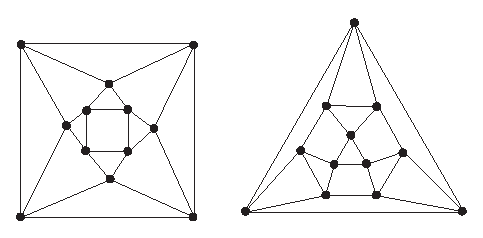
\includegraphics{PS/gfcchcp.eps}
  \caption{The plane graphs $G_{fcc}$ and $G_{hcp}$}
  \label{fig:gfcchcp}
\end{figure}

There is one more tame plane graph that is particularly troublesome.
It is the graph $G_{pent}$\index{pentahedral prism} obtained from
the pictured configuration of twelve balls tangent to a given
central ball (Figure \ref{fig:pentahedral}). (Place a ball at the
north pole, another at the south pole, and then form two pentagonal
rings of five balls.) This case requires individualized attention.
S. Ferguson\index{Ferguson} proves the following theorem in
\shortversion{his thesis \cite{thesis}.}
\longversion{\Part~\ref{part:ferguson}.}

\begin{theorem} [Ferguson] \label{lemma:ferguson}
There are no contravening decomposition stars $D$ whose associated
plane graph is isomorphic to $G_{pent}$.
\end{theorem}


\begin{figure}[htb]
  \centering
  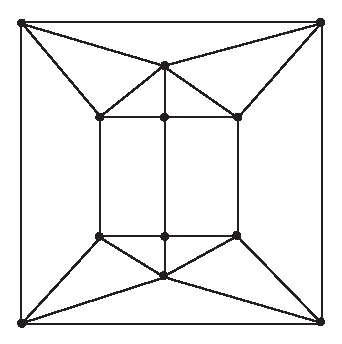
\includegraphics{PS/gpent.eps}
  \caption{The plane graph $G_{pent}$}\index{pentahedral prism}
   of the pentahedral prism.
  \label{fig:pentahedral}
\end{figure}

\section{Logical Skeleton of the Proof}
\label{sec:logic}

Consider the following six claims.  Eventually we will give a
proof of all six statements.  First, we draw out some of their
consequences.  The main results (Theorems~\ref{theorem:kepler},
\ref{theorem:sigma}, and \ref{theorem:sharp}) all follow from
these claims.

\begin{claim}\label{claim-A}
If the maximum of the function $\sigma$ on $\op{DS}$ is $8\,\pt$,
then for every saturated packing $\Lambda$ there exists a
negligible fcc-compatible function $A$.
\end{claim}

\begin{claim}\label{claim-B}
Let $D$ be a contravening decomposition star. Then its plane graph
$G(D)$ is tame.
\end{claim} %\ref{theorem:contravene} in kepler.tex

\begin{claim}\label{claim-C}
If a plane graph is tame, then it is isomorphic to one of the
several thousand plane graphs that appear in the archival list of
plane graphs.
\end{claim} %\ref{theorem:classification} in kepler.tex

\begin{claim}\label{claim-D}
If the plane graph of a contravening
decomposition star is isomorphic to one in the archival list of
plane graphs, then it is isomorphic to one of the following three
plane graphs: $G_{pent}$, $G_{hcp}$, or $G_{fcc}$.
\end{claim} %\label{lemma:fcc-hcp-pent} in linprog.tex

\begin{claim}\label{claim-E}
There do not exist any contravening decomposition stars
$D$ whose associated graph is isomorphic to $G_{pent}$.
\end{claim} %\label{lemma:ferguson} in form.tex

\begin{claim}\label{claim-F}
Contravening decomposition stars exist.
If $D$ is a contravening
decomposition star, and if the plane graph of $D$ is isomorphic to
$G_{fcc}$ or $G_{hcp}$, then $\sigma(D) = 8\,\pt$.  Moreover, up
to Euclidean motion, $U(D)$ is the kissing arrangement of the $12$
balls around a central ball in the face-centered cubic packing or
the kissing arrangement of $12$ balls in the hexagonal-close
packing.
\end{claim} %\label{lemma:local-optimality} in local_opt.tex

Next, we state some of the consequences of these claims.

\begin{lemma}\label{lemma:claim-fcc-graph}
Assume Claims~\ref{claim-B}, \ref{claim-C}, \ref{claim-D}, and
\ref{claim-E}. If $D$ is a contravening decomposition star, then
its plane graph $G(D)$ is isomorphic to $G_{hcp}$ or $G_{fcc}$.
\end{lemma}

\begin{proof} Assume that $D$ is a contravening decomposition
star.  Then its plane graph is tame, and consequently appears on
the archival list of plane graphs.  Thus, it must be isomorphic to
one of $G_{fcc}$, $G_{hcp}$, or $G_{pent}$.  The final graph is
ruled out by Claim~\ref{claim-E}.
\end{proof}

\begin{lemma}\label{lemma:claim-sigma}
Assume Claims~\ref{claim-B}, \ref{claim-C}, \ref{claim-D},
\ref{claim-E}, and \ref{claim-F}. Then Theorem~\ref{theorem:sigma}
holds.
\end{lemma}

\begin{proof}
By Claim~\ref{claim-F} and Lemma~\ref{lemma:claim-fcc-graph}, the
value $8\,\pt$ lies in the range of the function $\sigma$ on
$\op{DS}$.   Assume for a contradiction that there exists a
decomposition star $D\in \op{DS}$ that has $\sigma(D)>8\,\pt$. By
definition, this is a contravening star. By
Lemma~\ref{lemma:claim-fcc-graph}, its plane graph is isomorphic
to $G_{hcp}$ or $G_{fcp}$.  By Claim~\ref{claim-F},
$\sigma(D)=8\,\pt$, in contradiction with $\sigma(D)>8\,\pt$.
\end{proof}

\begin{lemma}\label{lemma:claim-sharp}
Assume Claims~\ref{claim-B}, \ref{claim-C}, \ref{claim-D},
\ref{claim-E}, and \ref{claim-F}.  Then
Theorem~\ref{theorem:sharp} holds.
\end{lemma}

\begin{proof}  By Theorem~\ref{theorem:sigma}, the maximum of
$\sigma$ on $\op{DS}$ is $8\,\pt$.  Let $D$ be a decomposition
star at which the maximum $8\,\pt$ is attained.  Then $D$ is a
contravening star. Lemma~\ref{lemma:claim-fcc-graph} implies that
the plane graph is isomorphic to $G_{hcp}$ or $G_{fcc}$.  The
hypotheses of Claim~\ref{claim-F} are satisfied.  The conclusion
of Claim~\ref{claim-F} is the conclusion of
Theorem~\ref{theorem:sharp}.
\end{proof}

\begin{lemma}
Assume Claims~\ref{claim-A}--\ref{claim-F}. Then the Kepler
conjecture (Theorem~\ref{theorem:kepler}) holds.
\end{lemma}

\begin{proof} As pointed out in Remark~\ref{remark:precise}, the precise
meaning of the Kepler conjecture is for every saturated packing
$\Lambda$, the essential supremum of $\delta(x,r,\Lambda)$ is at
most $\pi/\sqrt{18}$.

Let $\Lambda$ be the set of centers of a saturated packing.  Let
$A:\Lambda \to \ring{R}$ be the negligible, fcc-compatible
function provided by Claim~\ref{claim-A} (and
Lemma~\ref{lemma:claim-sigma}). By Lemma~\ref{lemma:deltabound},
the function $A$ leads to a constant $C$ such that for all $r\ge
1$ and all $x\in \ring{R}^3$, the density $\delta(x,r,\Lambda)$
satisfies
   $$\delta(x,r,\Lambda) \le \pi/\sqrt{18} + C/r.$$
This implies that the essential supremum of $\delta(x,r,\Lambda)$
is at most $\pi/\sqrt{18}$.
\end{proof}

\begin{remark}
One other theorem (Theorem~\ref{lemma:negligible'}) was stated
without proof in Section~\ref{sec:statement}.  This result was
placed there to motivate the other results.  However, it is not an
immediate consequence of Claims~\ref{claim-A}--\ref{claim-F}.  Its
proof appears in Theorem~\ref{lemma:negligible}.
\end{remark}

\section{Proofs of the Central Claims}

The previous section showed that the main results in the
introduction (Theorems~\ref{theorem:kepler}, \ref{theorem:sigma},
and \ref{theorem:sharp}) follow from six claims. This section
indicates where each of these claims is proved, and mentions a few
facts about the proofs.

Claim~\ref{claim-A} is proved in Theorem~\ref{lemma:exista}.
Claim~\ref{claim-B} is proved in Theorem~\ref{theorem:contravene}.
Claim~\ref{claim-C}, the classification of tame graphs, is proved in
Theorem~\ref{theorem:classification}. By the classification of such
graphs, this reduces the proof of the Kepler conjecture to the
analysis of the decomposition stars attached to the finite explicit
list of tame plane graphs.  We will return to Claim~\ref{claim-D} in
a moment.  Claim~\ref{claim-E} is Ferguson's thesis, cited as
Theorem~\ref{lemma:ferguson}.

Claim~\ref{claim-F} is the local optimality of the face-centered
cubic and hexagonal close packings.   In
\Chap~\ref{sec:local-opt}, the necessary local analysis is carried
out to prove Claim~\ref{claim-F} as
Corollary~\ref{lemma:local-optimality2}.

%\begin{lemma}
%A decomposition star whose plane graph is $G_{fcc}$ or $G_{hcp}$ has
%    $$\sigma(D) \le 8\,\pt,$$
%with equality precisely when the decomposition star belongs to
%$\op{DS}_{crit}$. \end{lemma}

%In light of this result, we prove Theorem \ref{theorem:sigma} and
%Theorem \ref{theorem:sharp} by proving that any decomposition star
%whose graph is tame and not equal to $G_{fcc}$ or $G_{hcp}$ is not
%contravening.

Now we return to Claim~\ref{claim-D}. This claim is proved as
Theorem~\ref{lemma:fcc-hcp-pent}.  The idea of the proof is the
following.  Let $D$ be a contravening decomposition star with
graph $G(D)$. We assume that the graph $G(D)$ is not isomorphic to
$G_{fcc}$, $G_{hcp}$, $G_{pent}$ and then prove that $D$ is not
contravening. This is a case-by-case argument, based on the
explicit archival list of plane graphs.

To eliminate these remaining cases, more-or-less generic arguments
can be used.  A linear program is attached to each tame graph $G$.
The linear program can be viewed as a linear relaxation of the
nonlinear optimization problem of maximizing $\sigma$ over all
decomposition stars with a given tame graph $G$. Because it is
obtained by relaxing the constraints on the nonlinear problem, the
maximum of the linear problem is an upper bound on the maximum of
the original nonlinear problem. Whenever the linear programming
maximum is less than $8\,\pt$, it can be concluded that there is
no contravening decomposition star with the given tame graph $G$.
This linear programming approach eliminates most tame graphs.

When a single linear program fails to give the desired bound, it
is broken into a series of linear programming bounds, by branch
and bound techniques.  For every tame plane graph $G$ other than
$G_{hcp}$, $G_{fcc}$, and $G_{pent}$,\index{pentahedral prism} we
produce a series of linear programs that establish that there is
no contravening decomposition star with graph $G$.

The \paper~is organized in the following way.
\Chaps~\ref{sec:construction} through \ref{sec:scoring} introduce
the basic definitions.  \Chap~\ref{sec:scoring} gives a proof of
Claim~\ref{claim-A}. \Chap~\ref{sec:local-opt} proves
Claim~\ref{claim-F}. \longversion{\Chaps~\ref{sec:fine} through
\ref{sec:fb} present the fundamental estimates.}
\Chaps~\ref{sec:def-and-class} through
\ref{sec:proof-classification} give a proof of Claim~\ref{claim-C}.
\Chaps~\ref{sec:startame} through \ref{sec:weight} give a proof of
Claim~\ref{claim-B}. \Chaps~\ref{sec:linearprogram} through
\ref{sec:branchbound} give a proof of Claim~\ref{claim-D}.
Claim~\ref{claim-E} (Ferguson's thesis) \shortversion{is to be
published as a separate paper.} \longversion{appears in
\Part~\ref{part:ferguson}.}


\chapter{Construction of the $Q$-system}
\label{sec:construction}

%This chapter has been written in a way that to be logically independent
%of the other papers in this series.  However, some of the results are
%technical lemmas that are required in other chapters. Thus, some of the
%results in this chapter may seem to be lacking in motivation. For
%motivation and a top-level view of the proof of the Kepler conjecture,
%the reader should consult Chapter~\ref{sec:overview}.  The reader is
%strongly encouraged to read that chapter first.  The paper \cite{CH}
%also gives an informal introduction to the proof that is less
%technically demanding than this paper.

%The ``program" to prove the Kepler conjecture has been changed somewhat
%from some of my earlier papers (see \cite{part1} and \cite{part2}).
%Hence, we do not rely on any definitions or ``program-related'' theorems
%from these papers.  However, we make free use of statements in pure
%geometry from those papers, when it is perfectly clear that these
%statements do not depend on any program-specific definitions or results.
%All program-specific results are proved from scratch in this paper,
%even when the proof is nearly identical to a proof found in one of these
%earlier papers.

It is useful to separate the parts of space of relatively high
packing density from the parts of space with relatively low packing
density.  The $Q$-system, which is developed in this \chap, is a
crude way of marking off the parts of space where the density is
potentially high.  The $Q$-system is a collection of simplices whose
vertices are points of the packing $\Lambda$. The $Q$-system is
reminiscent of the Delaunay decomposition, in the sense of being a
collection of simplices with vertices in $\Lambda$.  In fact, the
$Q$-system is the remnant of an earlier approach to the Kepler
conjecture that was based entirely on the Delaunay decomposition
(see \cite{remarks}).  However, the $Q$-system differs from the
Delaunay decomposition in crucial respects.  The most fundamental
difference is that the $Q$-system, while consisting of
nonoverlapping simplices, does not partition all of space.

This \chap\ defines the set of simplices in the $Q$-system and
proves that they do not overlap.  In order to prove that the
simplices in the $Q$-system do not overlap,  we develop a long
series of lemmas that study the geometry of intersections of
various edges and simplices.  At the end of this \chap, we give
the proof that the simplices in the $Q$-system do not overlap.

\section{Description of the $Q$-system}
\label{sec:Q-describe}



Fix a packing of balls of radius $1$. We identify the packing with
the set $\Lambda$ of its centers.  A packing is thus a subset
$\Lambda$ of $\ring{R}^3$ such that for all $v,w\in\Lambda$,
$|v-w|<2$ implies $v=w$. The centers of the balls are called {\it
\index{vertex} vertices}. The term `vertex' will be reserved for
this technical usage.  A packing is said to be {\it
\index{saturated} saturated\/} if for every $x\in\ring{R}^3$,
there is some $v\in\Lambda$ such that $|x-v|<2$. Any packing is a
subset of a saturated packing. We assume that $\Lambda$ is
saturated. The set $\Lambda$ is countably infinite.

\begin{definition}  We define the {\it truncation parameter}
\index{truncation parameter ($t_0=1.255$)} to be the constant
$t_0=1.255$. It is used throughout. Informal arguments that led to
this choice of constant are described in
\longversion{\Part~\ref{part:intro}}\shortversion{\cite{KC}}.
\end{definition}

Precise constructions that rely on the truncation parameter $t_0$
will appear below.  We will regularly intersect Voronoi cells with
balls of radius $t_0$ to obtain lower bounds on their volumes.  We
will regularly disregard vertices of the packing that lie at
distance greater than $2t_0$ from a fixed $v\in\Lambda$ to obtain
a finite subset of $\Lambda$ (a finite cluster of balls in the
packing) that is easier to analyze than the full packing
$\Lambda$.

The truncation parameter is the first of many decimal constants
that appear. Each decimal constant is an exact rational value,
e.g. $2t_0 = 251/100$.  They are not to be regarded as
approximations of some other value.

\begin{definition}
A {\it quasi-regular\/} triangle\index{quasi-regular triangle} is
a set $T\subset \Lambda$ of three vertices such that if $v,w\in T$
then $|w-v|\le2t_0$. \end{definition}

\begin{definition}
A \index{simplex} simplex\index{simplex} is a set of four
vertices.
%The
%edge-lengths of a simplex $S$ are the lengths $|w-v|$ for $w,v\in
%S$ and $w\ne v$.
A {\it quasi-regular\/} tetrahedron is a simplex $S$ such that if
$v,w\in S$ then $|w-v|\le 2t_0$. A {\it quarter\/} is a simplex
whose edge lengths $y_1,\ldots,y_6$ can be ordered to satisfy
$2t_0\le y_1\le\sqr8$, $2\le y_i\le 2t_0$, $i=2,\ldots,6$. If a
quarter satisfies the strict inequalities $2t_0< y_1< \sqrt8$,
then we say that it is a strict quarter. We call the longest edge
$\{v,w\}$ of a quarter its {\it \index{diagonal} diagonal\/}. When
the quarter is strict, we also say that its diagonal is strict.
When the quarter has a distinguished vertex, the quarter is {\it
upright\/} if the distinguished vertex is an endpoint of the
diagonal, and {\it flat\/} otherwise.
\end{definition}
\index{quarter!strict} \index{quarter!upright}
\index{quarter!flat} \index{quasi-regular}
\index{quasi-regular!triangle} \index{quasi-regular!tetrahedron}

At times, we identify a simplex with its convex hull. We will say,
for example, that the circumcenter of a simplex is contained in
the simplex to mean that the circumcenter is contained in the
convex hull of the four vertices.  Similar remarks apply to
triangles, quasi-regular tetrahedra, quarters, and so forth.  We
will write $|S|$ for the convex hull of $S$ when we wish to be
explicit about the distinction between $|S|$ and its set of
extreme points.

When we wish to give an order on an edge, triangle, simplex, etc.
we present the object as an ordered tuple rather than a set. Thus,
we refer to both $(v_1,\ldots,v_4)$ and $\{v_1,\ldots,v_4\}$ as
simplices, depending on the needs of the given context.

\begin{definition}\index{overlap}
Two manifolds with boundary {\it overlap\/} if their interiors
intersect.
\end{definition}


\begin{definition}  A set $O$ of six vertices is
called a {\it quartered \index{octahedron} octahedron}, if there are
four pairwise nonoverlapping strict quarters $S_1,\ldots,S_4$ all
having the same diagonal, such that $O$ is the union of the four
sets $S_i$ of four vertices.  (It follows easily that the strict
quarters $S_i$ can be given a cyclic order with respect to which
each strict quarter $S_i$ has a face in common with the next, so
that a quartered octahedron is literally a octahedron that has been
partitioned into four quarters.)
\end{definition}

\begin{remark}\label{def:oct-order}
A quartered octahedron may have more than one diagonal of length
less than $\sqr8$, so its decomposition into four strict quarters
need not be unique.  The choice of diagonal has no particular
importance.  Nevertheless, to make things canonical, we pick the
diagonal of length less than $\sqrt8$ with an endpoint of smallest
possible value with respect to the lexicographical ordering on
coordinates; that is, with respect to the ordering $(y_1,y_2,y_3)
< (y_1',y_2',y_3')$, if $y_i=y'_i$, for $i=1,\ldots,k$, and
$y_{k+1}<y'_{k+1}$.  This selection rule for diagonals is fully
translation invariant in the sense that if one octahedron is a
translate of another (whether or not they belong to the same
saturated packing), then the selected diagonal of one is a
translate of the selected diagonal of the other.
\end{remark}

%An {\it octahedral ordering} of a saturated packing is a function
%that assigns a choice of diagonal of length less than $\sqrt8$ to
%each quartered octahedron.  We fix once and for all an octahedral
%ordering of every saturated packing.  We may assume that the
%choice is fully translation invariant in the sense that if
%$\Lambda$ and $\Lambda'$ are any two saturated packings (not
%necessarily distinct) and one contains an octahedron that is a
%translation of an octahedron in the other, then the choice of
%diagonal in one is a translation of the choice in the other.  One
%such (translation invariant) ordering would be the diagonal with
%an endpoint with the smallest possible value with respect to the
%lexicographical ordering on the coordinates.


%This choice of distinguished diagonal is entirely immaterial for
%the proof of the Kepler conjecture.  However, we wish to assert
%that certain constructions are canonical.  For that reason, we
%prefer to avoid basing our choice of diagonal on an arbitrary
%well-ordering of the diagonals. However, there are various rules
%for picking out one diagonal that do not involved any arbitrary
%choices and that rely instead on suitable lexicographical
%orderings of the edge-lengths in the octahedron. A canonical rule
%will be translation and rotation invariant.  Such a rule can be
%designed so that it always selects a diagonal of length less than
%$\sqrt8$ whenever such a diagonal exists.  Of course, any
%canonical rule based on edge-lengths will be invariant under the
%group of isometries of the octahedron, any cannot select a
%distinguished diagonal from a regular octahedron. However, a
%regular octahedron with sides at least $2$ has diagonals of length
%at least $\sqrt8$, and it therefore not a quartered octahedron. To
%avoid excess pedantry, we will not spell out a rule in detail.
% FALSE! Cannot always break the symmetry between the two shorter diags.



\begin{definition} \label{def:anchor}
If $\{v_1,v_2\}$ is an edge of length between $2t_0$ and $\sqr8$,
we say that a vertex $v$ $(\ne v_1,v_2)$ is an {\it \index{anchor}
anchor\/} of $\{v_1,v_2\}$ if its distances to $v_1$ and $v_2$ are
at most $2t_0$.
%
\end{definition}

The two vertices of a quarter that are not on the diagonal are
anchors of the diagonal, and the diagonal may have other anchors
as well.

\begin{definition}\label{def:q-system}
Let $\CalQ$ be the set of quasi-regular tetrahedra and strict
quarters, enumerated as follows. This set is called the
$Q$-system.  It is canonically associated with a saturated packing
$\Lambda$.  (The $Q$ stands for quarters and quasi-regular
tetrahedra.)
%
  \index{Q-system@$Q$-system}


\begin{enumerate}
   \item All quasi-regular tetrahedra.
   \item Every strict quarter such that none of the quarters along
   its diagonal overlaps any other
   quasi-regular tetrahedron or strict quarter.
   \item Every strict quarter whose diagonal has four or more
   anchors, as long as there are not exactly four anchors arranged
   as a quartered
   octahedron.
   \item The fixed choice of four strict quarters in each
   quartered octahedron.
   %\item Assume a strict quarter does not overlap a quasi-regular tetrahedron,
   %overlaps at least one other strict quarter,
   % and is not part of a quartered octahedron.  Of these, we include
   %\begin{enumerate}
   \item Every strict quarter $\{v_1,v_2,v_3,v_4\}$ whose diagonal
      $\{v_1,v_3\}$ has exactly three anchors $v_2$, $v_4$, $v_5$ provided that
      the following hold (for some choice of indexing).
      (a) $\{v_2,v_5\}$ is a strict diagonal
      with exactly three anchors: $v_1$, $v_3$, $v_4$.
      (b) $d_{24}+d_{25}>\pi$, where $d_{24}$ is the dihedral angle
       of the simplex $\{v_1,v_3,v_2,v_4\}$ along the edge $\{v_1,v_3\}$
       and $d_{25}$ is the dihedral angle of the simplex
       $\{v_1,v_3,v_2,v_5\}$ along the edge $\{v_1,v_3\}$.
       %The sum of the dihedral
       %  angles $\dih(v_1,v_3,v_2,v_4)+\dih(v_1,v_3,v_2,v_5)$ is
       %  greater than $\pi$.
   %\end{enumerate}
\end{enumerate}
No other quasi-regular tetrahedra or strict quarters are included
in the $Q$-system $\CalQ$.
\end{definition}


The following theorem is the main result of this \chap.

\begin{theorem}\label{thm:nonoverlap}
For every saturated packing, there exists a uniquely determined
$Q$-system.  Distinct simplices in the $Q$-system have disjoint
interiors.
\end{theorem}

While proving the theorem, we give a complete classification of
the various ways in which one quasi-regular tetrahedron or strict
quarter can overlap another.

Having completed our primary purpose of showing that the simplices
in the $Q$-system do not overlap, we state the following small
lemma. It is an immediate consequence of the definitions, but
which is nonetheless useful in the \chaps\ that follow.

\begin{lemma} \label{lemma:diags-engulf}
If one quarter along a diagonal lies in the $Q$-system, then all
quarters along the diagonal lie in the $Q$-system.
\end{lemma}

\begin{proof} This is true by construction.  Each of the defining properties
of a quarter in the $Q$-system is true for one quarter along a
diagonal if and only if  it is true of all quarters along the
diagonal.
\end{proof}


\section{Geometric Considerations}
    \label{sec:decomposition}

\begin{remark}  The primary definitions and
constructions of this paper are translation invariant.  That is,
if $\lambda\in\ring{R}^3$ and $\Lambda$ is a saturated packing,
then $\lambda+\Lambda$ is a saturated packing.  If
$A:\Lambda\to\ring{R}$ is a negligible fcc-compatible function for
$\Lambda$, then $\lambda+v\mapsto A(v)$ is a negligible
fcc-compatible function for $\lambda+\Lambda$.  If $\CalQ$ is the
$Q$-system of $\Lambda$, then $\lambda+\CalQ$ is the $Q$-system of
$\lambda+\Lambda$. Because of general translational invariance,
when we fix our attention on a particular $v\in\Lambda$, we will
often assume (without loss of generality) that the coordinate
system is fixed in such a way that $v$ lies at the origin.
\end{remark}

Our simplices are generally assumed to come labeled with a
distinguished vertex, fixed  at the origin. (The origin will
always be at a vertex of the packing.) We number the edges of each
simplex $1,\ldots,6$, so that edges $1$, $2$, and $3$ meet at the
origin, and the edges $i$ and $i+3$ are opposite, for $i=1,2,3$.
(See Figure~\ref{fig:diag11}.)  $S(y_1,y_2,\ldots,y_6)$ denotes a
simplex whose edges have lengths $y_i$, indexed in this way. We
refer to the endpoints away from the origin of the first, second,
and third edges as the first, second, and third vertices.
%
 \index{labels!edge}
 \index{first!edge}

\begin{definition}\label{def:dih}
In general, let $\dih(S)$ be the dihedral angle of a simplex $S$
along its first edge. When we write a simplex in terms of its
vertices $(w_1,w_2,w_3,w_4)$, then $\{w_1,w_2\}$ is understood to
be the first edge.
%
 \index{dih (dihedral angle)}
\end{definition}

\begin{definition}
We define the {\it radial projection\/} of a set $X$ to be the
radial projection $x\mapsto x/|x|$ of $X\setminus{0}$ to the unit
sphere centered at the origin. We say the two sets {\it cross\/}
if their radial projections to the unit sphere
overlap.\index{projection of a set}
%
 \index{cross}
 \index{radial projection}
\end{definition}


\begin{definition}
    \label{def:calE}
If $S$ and $S'$ are nonoverlapping simplices with a shared face $F$,
we define $\CalE(S,S')$ as the distance between the two vertices
(one on $S$ and the other on $S'$) that do not lie on $F$.  We may
express this as a function
   $$\CalE(S,S')=\CalE(S(y_1,\ldots,y_6),y_1',y_2',y_3')$$
of nine variables, where $S=S(y_1,\ldots,y_6)$  and
$S'=S(y_1',y_2',y_3',y_4,y_5,y_6)$, positioned so that $S$ and $S'$
are nonoverlapping simplices with a shared face $F$ of edge-lengths
$(y_4,y_5,y_6)$.   The function of nine variables is defined only
for values $(y_i,y_i')$ for which the simplices $S$ and $S'$ exist.
(Figure~\ref{fig:diag11}).
\end{definition}

\begin{figure}[htb]
  \centering
  \includegraphics{PS/calE.eps}
  \caption{$\CalE$ measures the distance between the vertices at $0$ and $v$.
   The standard indexing of the edges of a simplex
   is marked on the lower simplex.}
  \label{fig:diag11}
\end{figure}

Several lemmas in this paper rely on calculations of lower bounds
to the function $\CalE$ in the special case when the edge between
the vertices $0$ and $v$ passes through the shared face $F$. If
intervals containing $y_1,\ldots,y_6,y_1',y_2',y_3'$ are given,
then lower bounds on $\CalE$ over that domain are generally easy
to obtain.  Detailed examples of calculations of the lower bound
of this function can be found in \cite[Sec. 4]{part1}.

To work one example, we suppose we are asked to give a lower bound
on $\CalE$ when the simplex $S=S(y_1,\ldots,y_6)$ satisfies
$y_i\ge2$ and $y_4,y_5,y_6\le 2t_0$ and
$S'=S(y'_1,y'_2,y'_3,y_4,y_5,y_6)$ satisfies $y'_i\ge2$, for
$i=1,\ldots,3$. Assume that the edge $\{0,v\}$ passes through the
face shared between $S$ and $S'$, and that $|v|<\sqrt8$, where $v$
is the vertex of $S'$ that is not on $S$.  We claim that any pair
$S,S'$ can be deformed by moving one vertex at a time until $S$ is
deformed into $S(2,2,2,2t_0,2t_0,2t_0)$ and $S'$ is deformed into
$S(2,2,2,2t_0,2t_0,2t_0)$.  Moreover, these deformations preserve
the constraints (including that $\{0,v\}$ passes through the shared
face), and is non-increasing in $|v|$.  From the existence of this
deformation, it follows that the original $|v|$ satisfies
   $$|v| \ge \CalE(S(2,2,2,2t_0,2t_0,2t_0),2,2,2).$$

We produce the deformation in this case as follows. We define the
{\it pivot\/} of a vertex $v$ with respect to two other vertices
$\{v_1,v_2\}$ as the circular motion of $v$ held at a fixed
distance from $v_1$ and $v_2$, leaving all other vertices fixed.
The {\it axis\/}\index{axis} of the \index{pivot} pivot is the
line through the two fixed vertices. Each pivot of a vertex can
move in two directions.  Let the vertices of $S$ be
$\{0,v_1,v_2,v_3\}$, labeled so that $|v_i|=y_i$.  Let
$S'=\{v,v_1,v_2,v_3\}$.  We pivot $v_1$ around the axis through
$0$ and $v_2$. By picking a suitable direction for the pivot,
$v_1$ moves away from $v$ and $v_3$. Its distance to $0$ and $v_2$
remains fixed. We continue with this circular motion until
$|v_1-v_3|$ achieves its upper bound or the segment $\{v_1,v_3\}$
intersects the segment $\{0,v\}$ (which threatens the constraint
that the segment $\{0,v\}$ pass through the common face).  (We
leave it as an exercise\footnote{Compare
Lemma~\ref{lemma:no-pass-sqrt2}.} to check that the second
possibility cannot occur because of the edge length upper bounds
on both diagonals of $\sqrt8$.  That is, there does not exist a
convex planar quadrilateral with sides at least $2$ and diagonals
less than $\sqrt8$.) Thus, $|v_1-v_3|$ attains its constrained
upper bound $2t_0$. Similar pivots to $v_2$ and $v_3$ increase the
lengths $|v_1-v_2|$, $|v_2-v_3|$, and $|v_3-v_1|$ to $2t_0$.
Similarly, $v$ may be pivoted around the axis through $v_1$ and
$v_2$ so as to decrease the distance to $v_3$ and $0$ until the
lower bound of $2$ on $|v-v_3|$ is attained.  Further pivots
reduce all remaining edge lengths to $2$.   In this way, we obtain
a rigid figure realizing the absolute lower bound of $|v|$.  A
calculation with explicit coordinates gives $|v|>2.75$.

Because lower bounds are generally easily determined from a series
of pivots through arguments such as this one, we will state them
without proof. We will state that these bounds were obtained by
{\it geometric considerations}, to indicate that the bounds were
obtained by the deformation arguments of this paragraph.
\index{geometric considerations}


\section{Incidence Relations}


\begin{lemma} \label{lemma:v-interior-alt}
Let $v,v_1,v_2,v_3$, and $v_4$ be distinct points in $\ring{R}^3$
with pairwise distances at least $2$.  Suppose that $|v_i-v_j|\le
2t_0$ for $i\ne j$ and $\{i,j\}\ne\{1,4\}$. Then $v$ does not lie
in the convex hull of $\{v_1,v_2,v_3,v_4\}$.
\end{lemma}

\begin{proof}
This lemma is proved in~\cite[Lemma 3.5]{part1}.
\end{proof}



\begin{lemma} \label{lemma:v-interior}
Let $S$ be a simplex whose edges have length between $2$ and
$2\sqrt2$.  Suppose that $v$ has distance at least $2$ from each
of the vertices of $S$.  Then $v$ does not lie in the convex hull
of $S$.
\end{lemma}

\begin{proof} Assume for a contradiction that $v$ lies in the
convex hull of $S$.   Place a unit sphere around $v$.  The simplex
$S$ partitions the unit sphere into four spherical triangles,
where each triangle is the intersection of the unit sphere with
the cone over a face of $S$, centered at $v$.   By the constraints
on the lengths of edges, the arclength of each edge of the
spherical triangle is at most $\pi/2$.  ($\pi/2$ is attained when
$v$ has distance $2$ to two of the vertices, and these two
vertices have distance $2\sqrt2$ between them.)  A spherical
triangle with edges of arclength at most $\pi/2$ has area at most
$\pi/2$.  In fact, any such spherical triangle can be placed
inside a octant of the unit sphere, and each octant has area
$\pi/2$. This partitions the sphere of area $4\pi$ into four
regions of area at most $\pi/2$. This is absurd.
\end{proof}

\bigskip
\begin{corollary}\label{cor:interior}
%{Lemma 1.2}
No vertex of the packing is contained in the convex hull of a
quasi-regular tetrahedron or quarter (other than the vertices of
the simplex).
\end{corollary}

\begin{proof}
The corollary is immediate.
\end{proof}


\begin{definition} \label{def:passes-through}
Let $v_1,v_2,w_1,w_2,w_3\in\Lambda$ be distinct.  We say that an
edge $\{v_1,v_2\}$ {\it passes through} the triangle
$\{w_1,w_2,w_3\}$ if the convex hull of $\{v_1,v_2\}$ meets some
point of the convex hull of $\{w_1,w_2,w_3\}$ and if that point of
intersection is not any of the extreme points $v_1$, $v_2$, $w_1$,
$w_2$, $w_3$.
%
 \index{passes through}
\end{definition}

\begin{lemma} \label{lemma:2t0-doesnt-pass-through}
%\proclaim{Lemma 1.3}
An edge of length $2t_0$ or less cannot pass through a triangle
whose edges have lengths $2t_0$, $2t_0$, and $\sqr8$ or less.
\end{lemma}

\begin{proof}  The distance between each pair of vertices is at least 2.
Geometric considerations show that the edge has length at least
$${\CalE}(S(2,2,2,2t_0,2t_0,\sqr8),2,2,2) > 2t_0.$$
\end{proof}

\begin{definition}\label{def:eta}\index{circumradius}
%
 \index{Zeta@$\eta$}
Let $\eta(x,y,z)$ denote the circumradius of a
triangle with edge-lengths $x$, $y$, and $z$.
\end{definition}


\begin{lemma}
\label{lemma:no-pass-sqrt2}
%{\bf Lemma I 3.2.}
Suppose that the circumradius of $\{v_1,v_2,v_3\}$ is less than
$\sqrt2$. Then an edge $\{w_1,w_2\}\subset\Lambda$ of length at
most $\sqr8$ cannot pass through the face.
\end{lemma}

\begin{proof}  Assume for a contradiction that $\{w_1,w_2\}$ passes through the
triangle $\{v_1,v_2,v_3\}$.   By geometric considerations, the
minimal length for $\{w_1,w_2\}$ occurs when $|w_i-v_j|=2$, for
$i=1,2$, $j=1,2,3$.  This distance constraint places the
circumscribing circle of $\{v_1,v_2,v_3\}$ on the sphere of radius
$2$ centered at $w_1$ (resp. $w_2$).  If $r<\sqrt2$ is the
circumradius of $\{v_1,v_2,v_3\}$, then for this extremal
configuration we have the contradiction
    $$\sqrt8\ge |w_1-w_2| = 2\sqrt{4-r^2}>\sqrt8.$$
\end{proof}

\begin{lemma} \label{lemma:qrtet-pair-pass}
%{Lemma 1.4}
If an edge of length at most $\sqrt{8}$ passes through a
quasi-regular triangle, then each of the two endpoints of the edge
is at most $2.2$ away from each of the vertices of the triangle
(see Figure~\ref{fig:dia31}).\index{quasi-regular!triangle}
\end{lemma}

\begin{figure}[htb]
  \centering
  \includegraphics{PS/dia31.ps}
  \caption{Frame (a) depicts two quasi-regular tetrahedra that share
  a face.  The same convex body may also be viewed as three quarters
  that share a diagonal, as in Frame (b).}
  \label{fig:dia31}
\end{figure}


\begin{proof}
Let the diagonal edge be $\{v_0,v_0'\}$ and the vertices of the
face be $\{v_1,v_2,v_3\}$.  If $|v_i-v_0|>2.2$ or $|v_i-v_0'|>2.2$
for some $i>0$, then geometric considerations give the
contradiction
$$|v_0-v_0'|\ge{\CalE}(S(2,2,2,2t_0,2t_0,2t_0),2,2,2.2) > \sqr8.$$
\end{proof}

%\begin{lemma}\label{lemma:2.15}
%Let $\{v_1,v_2,v_3\}$ be a quasi-regular triangle.  Assume that there is
%a vertex $v$ such that the distance from $v$ to the circumcenter is less
%than the circumradius.  Then $|v-v_i|\le2.15$, for $i=1,2,3$.  In
%particular, $\{v,v_1,v_2,v_3\}$ is a quasi-regular tetrahedron.
%\end{lemma}
%
%\begin{proof} This is proved in \cite[Lemma~3.4]{part1}.
%\end{proof}

\begin{lemma}\label{lemma:qrtet-quarter}
Suppose $S$ and $S'$ are quasi-regular tetrahedra that share a
face.  Suppose that the edge $e$ between the two vertices that are
not shared has length at most $\sqrt8$.   Then the convex hull of
$S$ and $S'$ consists of three quarters with diagonal $e$.  No
other quarter overlaps $S$ or $S'$.
\end{lemma}

\begin{proof}
Suppose that $S$ and $S'$ are adjacent quasi-regular tetrahedra
with a common face $F$.   By the
Lemma~\ref{lemma:qrtet-pair-pass}, each of the six external faces
of this pair of quasi-regular tetrahedra has circumradius at most
$\eta(2.2,2.2,2t_0)<\sqr2$. A diagonal of a quarter  cannot pass
through a face of this size by Lemma~\ref{lemma:no-pass-sqrt2}.
This implies that no other quarter overlaps these quasi-regular
tetrahedra.
\end{proof}


\begin{lemma} \label{lemma:pass-anchor}
%\proclaim{Lemma 1.5}
Suppose an edge $\{w_1,w_2\}$ of length at most $\sqr8$ passes
through the face formed by a diagonal $\{v_1,v_2\}$ and one of its
anchors. Then $w_1$ and $w_2$ are also anchors of $\{v_1,v_2\}$.
\end{lemma}

\begin{proof}  This follows from
the inequality
  $${\CalE}(S(2,2,2,\sqr8,2t_0,2t_0),2,2,2t_0) > \sqr8$$
and geometric considerations.
\end{proof}


\begin{definition} \label{def:height}  Let $\Lambda$ be a
saturated packing.  Assume that the coordinate system is fixed in
such a way that the origin is a vertex of the packing.  The {\it
height\/} of a vertex is its distance from the
origin.
%
 \index{height}
\end{definition}

\begin{definition} \label{def:enclosed}\index{enclosed}
We say that a vertex is {\it enclosed\/} over a figure
if it lies in the interior of the
cone at the origin generated by the figure.
%
 \index{vertex!enclosed}\index{enclosed}
\end{definition}


\begin{definition} \label{def:corner}
An {\it adjacent pair of quarters} consists of two quarters
sharing a face along a common diagonal. The common vertex that
does not lie on the diagonal is called the {\it base point\/} of
the adjacent pair.  (When one of the quarters comes with a marked
distinguished vertex, we do {\it not\/} assume that this marked
vertex coincides with the base point of the pair.)  The other four
vertices are called the {\it corners\/}  of the configuration.
%
 \index{adjacent pair}
 \index{base point}
 \index{corner}
\end{definition}

\begin{definition}
If the two corners, $v$ and $w$, that do not lie on the diagonal
satisfy $|w-v|<\sqrt8$, then the base point and four corners can
be considered as an adjacent pair in a second way, where $\{v,w\}$
functions as the diagonal.  In this case we say that the original
diagonal and the diagonal $\{v,w\}$ are {\it conflicting
diagonals}.\index{conflicting diagonal} %
\end{definition}

\begin{definition}
A quarter is said to be {\it isolated}\index{isolated} if it
is not part of an adjacent pair.  Two isolated quarters that
overlap are said to form an {\it isolated
pair}.\index{pair!isolated}
%
\end{definition}

\begin{lemma} \label{lemma:skew-quad}
%\proclaim{Lemma 1.6}
Suppose that there exist four nonzero vertices $v_1,\ldots,v_4$ of
height at most $2t_0$ (that is, $|v_i|\le 2t_0$) forming a skew
quadrilateral. Suppose that the diagonals $\{v_1,v_3\}$ and
$\{v_2,v_4\}$ have lengths between $2t_0$ and $\sqr8$. Suppose the
diagonals $\{v_1,v_3\}$ and $\{v_2,v_4\}$ cross. Then the four
vertices are the corners of an adjacent pair of quarters with base
point at the origin.
\end{lemma}

\begin{proof}
 Set $d_1=|v_1-v_3|$ and $d_2 = |v_2-v_4|$.
By hypothesis, $d_1$ and $d_2$ are at most $\sqr8$.
 If $|v_1-v_2|>2t_0$,
geometric considerations give the contradiction
    $$\max(d_1,d_2)\ge \CalE(S(2t_0,2,2,2t_0,\sqr8,2t_0),2,2,2) > \sqr8
    \ge\max(d_1,d_2).$$
Thus, $\{0,v_1,v_2\}$ is a quasi-regular triangle,  as are
$\{0,v_2,v_3\}$, $\{0,v_3,v_4\}$, and $\{0,v_4,v_1\}$ by symmetry.
\end{proof}

\begin{lemma} \label{lemma:oct}
%\proclaim{Lemma 1.7}
If, under the same hypotheses as Lemma~\ref{lemma:skew-quad},
there is a vertex $w$ of height at most $\sqr8$ enclosed over the
adjacent pair of quarters, then $\{0,v_1,\ldots,v_4,w\}$ is a
quartered octahedron.
\end{lemma}


\begin{proof}
 If the enclosed $w$ lies over say $\{0,v_1,v_2,v_3\}$, then
$|w-v_1|$, $|w-v_3|\le 2t_0$ (Lemma~\ref{lemma:pass-anchor}), where
$\{v_1,v_3\}$ is a diagonal. Similarly, the distance from $w$ to the
other two corners is at most $2t_0$.
\end{proof}

\begin{lemma} \label{lemma:double-face}
%proclaim{Lemma 1.8}
Let $v_1$ and $v_2$ be anchors of $\{0,w\}$ with $2t_0\le |w|\le
\sqr8$. If an edge $\{v_3,v_4\}$ passes through both faces,
$\{0,w,v_1\}$ and $\{0,w,v_2\}$, then $|v_3-v_4|>\sqr8$.
\end{lemma}

\begin{proof}
Suppose the figure exists with $|v_3-v_4|\le\sqr8$. Label vertices
so $v_3$ lies on the same side of the figure as $v_1$. Contract
$\{v_3,v_4\}$ by moving $v_3$ and $v_4$ until
    $\{v_i,u\}$ has length $2$,
for $u=0,w,v_{i-2}$, and $i=3,4$. Pivot $w$ away from $v_3$ and
$v_4$ around the axis $\{v_1,v_2\}$ until
    $|w|=\sqr8$.
Contract $\{v_3,v_4\}$ again. By stretching $\{v_1,v_2\}$, we
obtain a square of edge two and vertices $\{0,v_3,w,v_4\}$. Short
calculations based on explicit formulas for the dihedral angle and
its partial derivatives give
    \begin{equation}
        \dih(S(\sqr8,2,y_3,2,y_5,2)) > 1.075,\quad
        y_3,y_5\in[2,2t_0],\label{eqn:1.7.1}
    \end{equation}
    %
    \begin{equation}
    \dih(S(\sqr8,y_2,y_3,2,y_5,y_6)) >1,\quad
        y_2,y_3,y_5,y_6\in[2,2t_0].
        \label{eqn:1.7.2}
    \end{equation}
Then
$$\pi\ge \dih(0,w,v_3,v_1) + \dih(0,w,v_1,v_2) + \dih(0,w,v_2,v_4)
    > 1.075 + 1 + 1.075 > \pi.$$
Therefore, the figure does not exist.
\end{proof}

\begin{lemma} \label{lemma:single-enclosed}
%proclaim{Lemma 1.11}
Two vertices $w,w'$ of height at most $\sqr8$ cannot be enclosed
over a triangle $\{v_1,v_2,v_3\}$ satisfying $|v_1-v_2|\le\sqrt8$,
$|v_1-v_3|\le 2t_0$, and $|v_2-v_3|\le 2t_0$.
\end{lemma}

\begin{proof}
For a contradiction, assume the figure exists. The long edge
$\{v_1,v_2\}$ must have length at least $2t_0$ by
Lemma~\ref{lemma:qrtet-pair-pass}. This diagonal has anchors
$\{0,v_3,w,w'\}$. Assume that the cyclic order of vertices around
the line $\{v_1,v_2\}$ is $0,v_3,w,w'$. We see that $\{v_1,w\}$ is
too short to pass through $\{0,v_2,w'\}$, and $w$ is not inside
the simplex $\{0,v_1,v_2,w'\}$.  Thus, the projections of the
edges $\{v_2,w\}$ and $\{0,w'\}$ to the unit sphere at $v_1$ must
intersect.  It follows that $\{0,w'\}$ passes through
$\{v_1,v_2,w\}$ or $\{v_2,w\}$ passes through $\{v_1,0,w'\}$.  But
$\{v_2,w\}$ is too short to pass through $\{v_1,0,w'\}$.  Thus,
$\{0,w'\}$ passes through both $\{v_1,v_2,w\}$ and
$\{v_1,v_2,v_3\}$. Lemma~\ref{lemma:double-face} gives the
contradiction $|w'|>\sqrt8$.
\end{proof}

\begin{lemma} \label{lemma:pass-makes-quarter}
%{Lemma 1.9}
Let $v_1,v_2,v_3$ be anchors of $\{0,w\}$, where
$2t_0\le|w|\le\sqr8$, $|v_1-v_3|\le\sqr8$, and the edge
$\{v_1,v_3\}$ passes through the face $\{0,w,v_2\}$.  Then
$\min(|v_1-v_2|,|v_2-v_3|)\le2t_0$. Furthermore, if the minimum is
$2t_0$, then $|v_1-v_2|=|v_2-v_3|=2t_0$.
\end{lemma}

\begin{proof}
Assume $\min\ge2t_0$. As in the proof of
Lemma~\ref{lemma:double-face}, we may assume that $(0,v_1,w,v_3)$
is a square.  We may also assume, without loss of generality, that
$|w-v_2|=|v_2|=2t_0$. This forces $|v_2-v_i|=2t_0$, for $i=1,3$.
This is rigid,  and is the unique figure that satisfies the
constraints. The lemma follows.
\end{proof}


\bigskip

\section{Overlap of Simplices}
\label{sec:nonoverlap}

This section gives a proof of Theorem~\ref{thm:nonoverlap}
(simplices in the $Q$-system do not overlap).  This is accomplished
in a series of lemmas.  The first of these treats quasi-regular
tetrahedra.


\begin{lemma} \label{lemma:qrtet-over}
A quasi-regular tetrahedron does not overlap any
other simplex in the $Q$-system.
\end{lemma}

\begin{proof} Edges of quasi-regular tetrahedra are too short to
pass through the face of another quasi-regular tetrahedron or
quarter (Lemma~\ref{lemma:2t0-doesnt-pass-through}).  If a
diagonal of a strict quarter passes through the face of a
quasi-regular tetrahedron, then Lemma~\ref{lemma:qrtet-quarter}
shows that the strict quarter is one of three joined along a
common diagonal.  This is not one of the enumerated types of
strict quarter in the $Q$-system.
\end{proof}

\begin{lemma} \label{lemma:oct-over}
A quarter in the $Q$-system that is part of a
quartered octahedron does not overlap any other simplex in the
$Q$-system.
\end{lemma}

\begin{proof} By construction, the quarters that lie along a
different diagonal of the octahedron do not belong to the
$Q$-system.  Edges of length at most $2t_0$ are too short to pass
through an external face of the octahedron
(Lemma~\ref{lemma:2t0-doesnt-pass-through}). A diagonal of a
strict quarter cannot pass through an external face either,
because of Lemma~\ref{lemma:qrtet-pair-pass}.
\end{proof}

\begin{lemma}\label{lemma:adj-over}
Let $Q$ be a strict quarter that is part of an adjacent pair.
Assume that $Q$ is not part of a quartered octahedron.  If $Q$
belongs to the $Q$-system, then it does not overlap any other
simplex in the $Q$-system.
\end{lemma}

The proof of this lemma will give valuable details about how one
strict quarter overlaps another.

\begin{proof}
Fix the origin at the base point of an adjacent pair of quarters.
We investigate the local geometry when another quarter overlaps
one of them.  (This happens, for example, when there is a
conflicting diagonal in the sense of Definition~\ref{def:corner}.)

%if both diagonals between opposite corners of the adjacent pair of
%quarters have lengths at most $\sqr8$.  We will see that a
%conflict like this between the diagonals between corners is the
%only way an adjacent pair of quarters can overlap another quarter.
%We call these {\it conflicting\/} diagonals.

Label the base point of the pair of quarters $v_0$, and the four
corners  $v_1$, $v_2$, $v_3$, $v_4$, with $\{v_1,v_3\}$ the common
diagonal. Assume that $|v_1-v_3|<\sqrt8$.\index{conflicting
diagonals}

If two quarters overlap then a face on one of them overlaps a face
on the other.  By Lemmas~\ref{lemma:single-enclosed} and
\ref{lemma:double-face}, we actually have that some edge (in fact
the diagonal) of each passes through a face of the other.  This
edge cannot exit through another face by
Lemma~\ref{lemma:double-face} and it cannot end inside the simplex
by Corollary~\ref{cor:interior}. Thus, it must end at a vertex of
the other simplex.  We break the proof into cases according to
which vertex of the simplex it terminates at. In Case 1, the edge
has the base point as an endpoint.  In Case 2, the edge has a
corner as an endpoint.

\noindent{\bf Case 1.} {\it The edge $\{0,w\}$ passes through the
triangle $\{v_1,v_2,v_3\}$, where $\{0,w\}$ is a diagonal of a
strict quarter.}

Lemma~\ref{lemma:pass-anchor} implies that $v_1$ and $v_3$ are
anchors of $\{0,w\}$. The only other possible anchors of $\{0,w\}$
are $v_2$ or $v_4$, for otherwise an edge of length at most $2t_0$
edge passes through a face formed by $\{0,w\}$ and one of its
anchors. If both $v_2$ and $v_4$ are anchors, then we have a
quartered octahedron, which has been excluded by the hypotheses of
the lemma.  Otherwise, $\{0,w\}$ has at most $3$ anchors: $v_1$,
$v_3$, and either $v_2$ or $v_4$. In fact, it must have exactly
three anchors, for otherwise there is no quarter along the edge
$\{0,w\}$. So there are exactly two quarters along the edge
$\{0,w\}$. There are at least four anchors along $\{v_1,v_3\}$:
$0$, $w$, $v_2$, and $v_4$.  The quarters along the diagonal
$\{v_1,v_3\}$ lie in the $Q$-system. (None of these quarters is
isolated.)  The other two quarters, along the diagonal $\{0,w\}$,
are not in the $Q$-system. They form an adjacent pair of quarters
(with base point $v_4$ or $v_2$) that has conflicting diagonals,
$\{0,w\}$ and $\{v_1,v_3\}$, of length at most $\sqr8$.

\noindent {\bf Case 2.}  {\it $\{v_2,v_4\}$ is a diagonal of
length less than $\sqr8$ (conflicting with $\{v_1,v_3\}$).}

(Note that if an edge of a quarter passes through the shared face
of an adjacent pair of quarters, then that edge must be
$\{v_2,v_4\}$, so that Case 1 and Case 2 are exhaustive.) The two
diagonals $\{v_1,v_3\}$ and $\{v_2,v_4\}$ do not overlap. By
symmetry, we may assume that $\{v_2,v_4\}$ passes through the face
$\{0,v_1,v_3\}$. Assume (for a contradiction) that both diagonals
have an anchor other than $0$ and the corners $v_i$. Let the
anchor of $\{v_2,v_4\}$ be denoted $v_{24}$ and that of
$\{v_1,v_3\}$ be $v_{13}$. Assume the figure is not a quartered
octahedron, so that $v_{13}\ne v_{24}$. By
Lemma~\ref{lemma:2t0-doesnt-pass-through}, it is impossible to
draw the edges $\{v_1,v_{13}\}$ and $\{v_{13},v_3\}$ between $v_1$
and $v_3$.  In fact, if the edges pass outside the quadrilateral
$\{0,v_2,v_{24},v_4\}$, one of the edges of length at most $2t_0$
(that is,
    $\{0,v_2\}$, $\{v_2,v_{24}\}$, $\{v_{24},v_4\}$,
or $\{v_4,0\}$) violates the lemma applied to the face
$\{v_1,v_3,v_{13}\}$. If they pass inside the quadrilateral, one of the
edges $\{v_1,v_{13}\}$, $\{v_{13},v_3\}$ violates the lemma applied to
the face
    $\{0,v_{2},v_4\}$ or $\{v_{24},v_2,v_4\}$.
We conclude that at most one of the two diagonals has additional
anchors.

If neither of the two diagonals has more than three anchors, we
have nothing more than two overlapping adjacent pairs of quarters
along conflicting diagonals.  The two quarters along the lower
edge $\{v_2,v_4\}$ lie in the $Q$-system.  Another way of
expressing this ``lower-edge'' condition is to require the two
adjacent quarters $Q_1$ and $Q_2$ satisfy
$\dih(Q_1)+\dih(Q_2)>\pi$, when the dihedral angles are measured
along the diagonal. The pair $(Q_1',Q_2')$ along the upper edge
will have $\dih(Q_1')+\dih(Q_2')<\pi$.

If there is a diagonal with more than three anchors,  the quarters
along the diagonal with more than three anchors lie in the
$Q$-system.  Any additional quarters along the diagonal
$\{v_2,v_4\}$ belong to an adjacent pair. Any additional quarters
along the diagonal $\{v_1,v_3\}$ cannot intersect the adjacent
pair along $\{v_2,v_4\}$.  Thus, every quarter intersecting an
adjacent pair also belongs to an adjacent pair.

In both possibilities of case 2, the two quarters left out of the
$Q$-system correspond to a conflicting diagonal.
\end{proof}

\begin{remark}\label{remark:iso}
We have seen in the proof of the Lemma~\ref{lemma:adj-over} that
if a strict quarter $Q$ overlaps a strict quarter that is part of
an adjacent pair, then $Q$ is also part of an adjacent pair. Thus,
if an isolated strict quarter overlaps another strict quarter,
then both strict quarters are necessarily isolated.
\end{remark}

\begin{lemma}\label{lemma:iso-over}
If an isolated strict quarter $Q$ overlaps another strict quarter,
then the diagonal of $Q$ has exactly three anchors.
\end{lemma}

The proof of the lemma will give detailed information about the
geometrical configuration that is obtained when an isolated
quarter overlaps another strict quarter.

\begin{proof}  Assume that there are two strict quarters $Q_1$ and $Q_2$
that overlap.  Following Remark~\ref{remark:iso}, assume that
neither is adjacent to another quarter. Let $\{0,u\}$ and
$\{v_1,v_2\}$ be the diagonals of $Q_1$ and $Q_2$. Suppose the
diagonal $\{v_1,v_2\}$ passes through a face $\{0,u,w\}$ of $Q_1$.
By Lemma~\ref{lemma:pass-anchor}, $v_1$ and $v_2$ are anchors of
$\{0,u\}$. Again, either the length of $\{v_1,w\}$ is at most
$2t_0$ or the length of $\{v_2,w\}$ is at most $2t_0$, say
$\{w,v_2\}$ (by Lemma~\ref{lemma:pass-makes-quarter}). It follows
that
    $Q_1=\{0,u,w,v_2\}$ and $|v_1-w|\ge2t_0$.
($Q_1$ is not adjacent to another quarter.)  So $w$ is not an anchor of
$\{v_1,v_2\}$.

Let $\{v_1,v_2,w'\}$ be a face of $Q_2$ with $w'\ne 0,u$. If
$\{v_1,w',v_2\}$ does not link $\{0,u,w\}$, then $\{v_1,w'\}$ or
$\{v_2,w'\}$ passes through the face $\{0,u,w\}$, which is
impossible by Lemma~\ref{lemma:2t0-doesnt-pass-through}. So
$\{v_1,v_2,w'\}$  links $\{0,u,w\}$ and an edge of $\{0,u,w\}$
passes through the face $\{v_1,v_2,w'\}$. It is not the edge
$\{u,w\}$ or $\{0,w\}$, for they are too short by
Lemma~\ref{lemma:2t0-doesnt-pass-through}.  So $\{0,u\}$ passes
through $\{w',v_1,v_2\}$. The only anchors of $\{v_1,v_2\}$ (other
than $w'$) are $u$ and $0$ (by Lemma~\ref{lemma:double-face}).
Either $\{u,w'\}$ or $\{w',0\}$ has length at most $2t_0$ by
Lemma~\ref{lemma:pass-makes-quarter}, but not both, because this
would create a quarter adjacent to $Q_2$. By symmetry,
$Q_2=\{v_1,v_2,w',0\}$ and the length of $\{u,w'\}$ is greater
than $2t_0$. By symmetry, $\{0,u\}$ has no other anchors either.
This determines the local geometry when there are two quarters
that intersect without belonging to an adjacent pair of quarters
(see Figure~\ref{fig:diag19}).  It follows that the two quarters
form an isolated pair.
\end{proof}

\begin{figure}[htb]
  \centering
  \includegraphics{PS/isolatedpair.eps}
  \caption{An isolated pair.  The isolated pair consists of two simplices
   $Q_1=\{0,u,w,v_2\}$ and $Q_2=\{0,w',v_1,v_2\}$.  The six extremal vertices
   form an octahedron. This is not a quartered octahedron because the edges
   $\{u,w'\}$ and $\{w,v_1\}$ have length greater than $2t_0$.}
  \label{fig:diag19}
\end{figure}


Isolated quarters that overlap another strict quarter do not
belong to the $Q$-system.



%
%By geometric considerations,
%reduce to the case where
%the vertices $w$ and $w'$ have height at most $\sqr8$ and
%are enclosed in the quarter $S(2,2,2,2t_0,2t_0,\sqr8)$.
%We may assume that $w$ and $w'$ each have distance
%2 from two of the vertices of the quarter.  There are two possibilities.
%In either case $w$ or $w'$ forms a quarter with a face of the flat quarter.
%By Lemmas 1.2, 1.4, 1.9, 1.10, this leaves nowhere for the other
%enclosed vertex to go. \qed\enddemo

%\begin{remark} \label{remark:def-q-system}
%We conclude this section with a summary of the rules determining the
%$Q$-system.  The preceding discussion shows that these rules can be
%consistently applied in a way that produces a set of nonoverlapping
%simplices.\index{Q-system}

%\begin{itemize}
%    \item Every simplex in the $Q$-system is a quasi-regular tetrahedron
%    or a strict quarter.
%    \item Every quasi-regular tetrahedron belongs to the $Q$-system.
%    \item If a quarter overlaps a quasi-regular tetrahedron, it does
%    not belong to the $Q$-system.
%    \item If a strict quarter does not overlap any other strict
%    quarter or quasi-regular tetrahedron,
%    then it
%    belongs to the $Q$-system.
%    \item If a quarter is part of an isolated pair, then it does not
%    belong to the $Q$-system.
%    \item For every quartered octahedron, pick one diagonal of length less than $\sqrt8$
%    and put the four quarters along
%    that diagonal in the $Q$-system, but not any of the quarters that
%    overlap these.
%    \item Suppose that a strict quarter does not overlap a quasi-regular
%    tetrahedron, does overlap at least one other strict quarter,
%    is not part of an isolated pair, and is not part of a
%    quartered octahedron.  It follows from the fact that
%    the quarter is not an
%    isolated pair, that the diagonal of the quarter has at least three anchors.
%        \begin{itemize}
%            \item If there are four or more anchors, then the
%            quarter $Q$ belongs to the $Q$-system.
%            \item If there are three anchors, and it overlaps a strict
%            quarter with more than three anchors, then $Q$ does not belong to the $Q$-system.
%            \item If there are three anchors and every strict
%            quarter it overlaps
%            also has three anchors, then by the
%            discussion above, there is exactly one other quarter $Q_2$ along the diagonal of $Q_1$.
%            The quarter $Q_1$ belongs to the $Q$-system if and only if
%                $\dih(Q_1)+\dih(Q_2)>\pi$.
%        \end{itemize}
%\end{itemize}
%\end{remark}

\bigskip

We conclude the \chap\ with the proof of the main theorem of the
\chap.

\begin{proof} {\bf (Theorem~\ref{thm:nonoverlap})}
The rules defining the $Q$-system specify a uniquely determined
set of simplices.  The proof that they do not overlap is
established by the preceding series of lemmas.
Lemma~\ref{lemma:qrtet-over} shows that quasi-regular tetrahedra
do not overlap other simplices in the $Q$-system.
Lemma~\ref{lemma:oct-over} shows that the quarters in quartered
octahedra are well-behaved. Lemma~\ref{lemma:adj-over} shows that
other quarters in adjacent pairs do not overlap other simplices in
the $Q$-system. Finally, we treat isolated quarters in
Lemma~\ref{lemma:iso-over}. These cases cover all possibilities
since every simplex in the $Q$-system is a quasi-regular
tetrahedron or strict quarter, and every strict quarter is either
part of an adjacent pair or isolated.
\end{proof}





\chapter{$V$-cells}
\label{sec:vcells}

In the proof of the Kepler conjecture we make use of two quite
different structures in space.  The first structure is the
$Q$-system, which was defined in the previous \chap.  It is inspired
by the Delaunay decomposition of space. It consists of a
nonoverlapping collection of simplices that have their vertices at
the points of $\Lambda$.  Historically, the construction of the
nonoverlapping simplices of the $Q$-system grew out of a detailed
investigation of the Delaunay decomposition.

The second structure is inspired by the Voronoi decomposition of
space. In the Voronoi decomposition, the vertices of $\Lambda$ are
the centers of the cells.  It is well known that the Voronoi
decomposition and Delaunay decomposition are dual to one another.
Our modification of Voronoi cells will be called $V$-cells.

In general, it is not true that a Delaunay simplex is contained in
the union of the Voronoi cells at its four vertices.  This
incompatibility of structures adds a few complications to Rogers's
elegant proof of a sphere packing bound \cite{Rogers}. In this
\chap, we show that $V$-cells are compatible with the $Q$-system
in the sense that each simplex in the  $Q$-system is contained in
the union of the $V$-cells at its four vertices
(Lemma~\ref{lemma:Q-divide}). A second compatibility result
between these two structures is proved in
Lemma~\ref{lemma:V-cell-local}.

The purpose of this \chap\ is to define $V$-cells and to prove the
compatibility results just mentioned.  In the proof of the Kepler
conjecture it will be important to keep both structures (the
$Q$-system and the $V$-cells) continually at hand. We will
frequently jump back and forth between these dual descriptions of
space in the course of the proof.  In \Chap~\ref{sec:compact}, we
define a geometric object (called the decomposition star) around a
vertex that encodes both structures.  The decomposition star will
become our primary object of analysis.


\section{$V$-Cells}
\label{sec:cells}




\begin{definition} \label{def:Voronoi}
    The \index{Voronoi cell} Voronoi cell
$\Omega(v)$ around a vertex $v\in\Lambda$ is the set of points
closer to $v$ than to any other vertex.
\end{definition}




\begin{definition}\label{def:barrier}
We construct a set of triangles $\CalB$ in the packing.  The
triangles in this set will be called {\it barriers}.\index{barrier}
A triangle $\{v_1,v_2,v_3\}$ with vertices in the packing belongs to
$\CalB$ if and only if  one or more of the following properties hold
of it.
\begin{enumerate}
    \item The triangle is a
    quasi-regular, or\index{quasi-regular!triangle}
    \item The triangle is a face of a simplex in the $Q$-system.
\end{enumerate}
\end{definition}

\begin{lemma}\label{lemma:barrier-no-overlap}
 No two barriers overlap; that is, no two open triangular regions of
 $\CalB$ intersect.
\end{lemma}

\begin{proof} If there is overlap, an edge $\{w_1,w_2\}$ of one triangle passes
through the interior of another $\{v_1,v_2,v_3\}$.  Since
$|w_1-w_2|<\sqrt8$,  we have that the circumradius of
$\{v_1,v_2,v_3\}$ is at least $\sqrt2$ by
Lemma~\ref{lemma:no-pass-sqrt2} and that the length $|w_1-w_2|$ is
greater than $2t_0$ by Lemma~\ref{lemma:2t0-doesnt-pass-through}.
If the edge $\{w_1,w_2\}$ belongs to a simplex in the $Q$-system,
the simplex must be a strict quarter.  If $\{v_1,v_2,v_3\}$ has
edge lengths at most $2t_0$, then
Lemma~\ref{lemma:qrtet-pair-pass} implies that $|w_i-v_j|\le2.2$
for $i=1,2$ and $j=1,2,3$.   The simplices $\{v_1,v_2,v_3,w_1\}$
and $\{v_1,v_2,v_3,w_2\}$ form a pair of quasi-regular tetrahedra.
We conclude that $\{v_1,v_2,v_3\}$ is a face of a quarter in the
$Q$-system. Since, the simplices in the $Q$-system do not overlap,
the edge $\{w_1,w_2\}$ does not belong to a simplex in the
$Q$-system. The result follows.
\end{proof}




\begin{definition} \label{def:obstructed}
We say that a point $y$ is {\it obstructed\/} at $x\in\ring{R}^3$
if the line segment from $x$ to $y$ passes through the interior of
a triangular region in $\CalB$. Otherwise, $y$ is unobstructed at
$x$.  The `obstruction' relation between $x$ and $y$ is clearly
symmetric.\index{obstructed}
\end{definition}

For each $w\in\Lambda$, let $I_w$ be the cube of side $4$, with
edges parallel to the coordinate axes, centered at $w$.  Thus,
   $$I_0 = \{(y_1,y_2,y_3) :  |y_i|\le 2,\quad i=1,2,3\}.$$
$I_w$ has diameter $4\sqrt3$ and $I_w\subset B(w,2\sqrt3)$.  Let
$\Rp$ be the subset of $x\in\ring{R}^3$ for which $x$ is not
equidistant from any two $v,w\in \Lambda(x,2\sqrt3)=
B(x,2\sqrt3)\cap\Lambda$. The subset $\Rp$ is dense in
$\ring{R}^3$, and is obtained locally around a point $x$ by
removing finitely many planes (perpendicular bisectors of
$\{v,w\}$, for $v,w\in B(x,2\sqrt3)$). For $x\in\Rp$, the vertices
of $\Lambda(x,2\sqrt3)$ can be strictly ordered by their distance
to $x$.

\begin{definition}\label{def:phi}
Let $\Lambda$ be a saturated packing. We define a map
$\phi:\Rp\to\Lambda$ such that the image of $x$ lies in
$\Lambda(x,2\sqrt3)$.   If $x\in \Rp$, let
   $$\Lambda_x = \{w\in\Lambda : x \in I_w \text{ and
      $w$ is unobstructed at $x$}\}.$$
If $\Lambda_x = \emptyset$, then let $\phi(x)$ be the vertex of
$\Lambda(x,2\sqrt3)$ closest to $x$.   (Since $\Lambda$ is
saturated, $\Lambda(x,2\sqrt3)$ is nonempty.)  If $\Lambda_x$ is
nonempty, then let $\phi(x)$ be the vertex of $\Lambda_x$ closest to
$x$.
\end{definition}

%\begin{remark} \label{def:phi}
%
%    The truncation $|v-x|\le4$ in the definition of $\Rp$ is
%    quite arbitrary.  We could replace $4$ with any sufficiently large
%    truncation constant $C$.  For example, $C=2^{100}$ would work just as well.  However,
%    there will be various mild constraints on the lower bound of $C$.
%    It should be at least $\eta(2,2t_0,\sqrt8)\approx 1.45$ and it
%    should be at least the circumradius of every simplex, all of
%    whose edges have length at most $\sqrt8$. (This gives $C\ge
%    \sqrt3$.)
%\end{remark}

\begin{definition}\label{def:vcell}
For $v\in\Lambda$, let $\op{VC}(v)$ be defined as the closure of
$\phi^{-1}(v)$ in $\ring{R}^3$.  We call it the {\it $V$-cell\/}
at $v$.\index{V-cell}\index{VZ@$VC(v)$ ($V$-cell)}
%
\end{definition}


\begin{remark}
In a saturated packing, the Voronoi cell at $v$ will be contained
in a ball centered at $v$ of radius $2$.  Hence $I_v$ contains the
Voronoi cell at $v$.  By construction, the $V$-cell at $v$ is
confined to the cube $I_v$.  The cubes $I_v$ were introduced into
the definition of $\phi$ with the express purpose of forcing
$V$-cells to be reasonably small.  Had the cubes been omitted from
the construction, we would have been drawn to frivolous questions
such as whether the closest unobstructed vertex to some
$x\in\ring{R}^3$ might be located in a remote region of the
packing.
\end{remark}


%By construction, $V$-cells at different vertices are disjoint and
%give a partition of the subset $\Rp$.  Because of the truncation
%in Remark~\ref{def:phi}, the $V$-cell at $v$ is contained in
%$B(v,4)$, a closed ball of radius $4$ at $v$.

The set of $V$-cells is our promised decomposition of space.

\begin{lemma} $V$-cells cover space.  The interiors of distinct
$V$-cells are disjoint.  Each $V$-cell is the closure of its
interior.
\end{lemma}

\begin{proof}  The sets $\phi^{-1}(v)$, for $v\in\Lambda$ cover
$\Rp$.  Their closures cover $\ring{R}^3$.  The other statements in
the lemma will follow from the fact that a $V$-cell is a union of
finitely many nonoverlapping closed convex polyhedra.  This is
proved below in Lemma~\ref{lemma:V-convex}.
\end{proof}

\begin{lemma}\label{lemma:V-convex}
Each $V$-cell is a finite union of nonoverlapping convex polyhedra.
\end{lemma}

\begin{proof}
During this proof, we ignore sets of measure zero in $\ring{R}^3$
such as finite unions of planes.  Thus, we present the proof as if
each point belongs to exactly one Voronoi cell, although this
fails on an inconsequential set of measure zero in $\ring{R}^3$.

It is enough to show that if $E\subset\ring{R}^3$ is an arbitrary
unit cube, then the $V$-cell decomposition of space within $E$
consists of finite unions of nonoverlapping convex polyhedra. Let
$X_E$ be the set of $w\in\Lambda$ such that $I_w$ meets $E$.
Included in $X_E$ is the set of $w$ whose Voronoi cells cover $E$.
The rules for $V$-cells assign $x\in E$ to the $V$-cell centered at
some $w\in X_E$.

Let $d$ be an upper bound on the distance between a vertex in
$X_E$ and a point of $E$. By the pythagorean theorem, we may take
$d=(1+2)\sqrt3$.  Let $B_E$ be the set of barriers with a vertex
at most distance $d$ from some point in $E$.

For each pair $\{u,v\}$ of distinct vertices of $X_E$, draw the
perpendicular bisecting plane of $\{u,v\}$.  Draw the plane
through each barrier in $B_E$. Draw the plane through each triple
$\{u,v,w\}$, where $u\in X_E$ and $\{v,w\}$ are two of the
vertices of a barrier in $B_E$. These finitely many planes
partition $E$ into finitely many convex polyhedra. The ranking of
distances from $x$ to the points of $X_E$ is constant for all $x$
in the interior of any fixed polyhedron.  The set of $w\in X_E$
that are obstructed at $x$ is constant on the interior of any
fixed polyhedron.  Thus, by the rules of construction of
$V$-cells, for each of these convex polyhedra, there is a $V$-cell
that contains it.  The result follows.
\end{proof}

\begin{remark}\label{remark:pathology}
A number of readers of the first version of this manuscript
presumed that $V$-cells were necessarily star-convex, in large
part because of the inapt name {\it `decomposition star'\/} for a
closely related object. The geometry of a $V$-cell is
significantly more complex than that of a Voronoi cell. Nowhere do
we make a general claim that all $V$-cells are convex,
star-convex, or even connected.  In Figure~\ref{fig:nonstar}, we
depict a hypothetical case in which the $V$-cell at $v$ is
potentially disconnected.  (This Figure is merely hypothetical,
because I have not checked whether it is possible to satisfy all
the metric constraints needed for it to exist.)  The shaded
triangle represents a barrier.  The point $x$ is obstructed by the
shaded barrier at $w$.  If $x$ and $y$ lie closer to $w$ than to
$v$, if $v$ is the closest unobstructed vertex to $x$, if $w$ is
the closest unobstructed vertex to $y$, if $x$, $y$, and $z$ are
all unobstructed at $v$, and if $z$ lies closer to $v$ than to
$w$, then it follows that $x$ and $z$ lie in the $V$-cell at $v$,
but that the intervening point $y$ does not.  Thus, if all of
these conditions are satisfied, the $V$-cell at $v$ is not
star-shaped at $v$.
\end{remark}


%At the same time, we
%do not make any claims to the contrary.
%This paper is intentionally silent on this issue.
%Figure~\ref{fig:nonstar} illustrates one potentially non-star
%convex situation.
%Figure~\ref{fig:nonstar} illustrates a situation that could
%potentially lead star-convexity to fail. Suppose that $v$ is the
%center of the $V$-cell and that $x$ is a point that belongs to the
%$V$-cell at $v$ even though it is closer to another vertex $w$.
%The vertex $w$ is obstructed at $x$ by a barrier $b$. If we move
%along the segment from $x$ to $v$, we reach a point $y$ that is no
%long obstructed at $w$. Thus, $y$ may belong the $V$-cell at
%$w$. As we move closer to $v$ along the same segment, we reach a
%point $z$ that is closer to $v$ than to $w$.  It belongs the
%$V$-cell at $v$. Thus, we see the potential for two points $z$ and
%$x$ to lie in the same $V$-cell, but to be separated by  points
%such as $y$ in a different $V$-cell.  Of course, pictures like
%this are suggestive of possibilities, but do not prove anything.
%\end{remark}

%   Warning: do not uncritically assume that $V$-cells are
%  star convex.  A proof of star-convexity would have to eliminate
%  possibilities such as the one illustrated.
% Might it not be possible for the points
%   $x$ (obstructed at $w$ by the shaded barrier)
%   and $z$ to belong to the $V$-cell
%   at $v$, even when an intermediate point $y$ belongs to the
%   $V$-cell at $w$?}

\begin{figure}[htb]
  \centering
  \includegraphics{PS/nonstar.eps}
  \caption{A hypothetical arrangement that leads to a nonconvex
   $V$-cell at $v$.}
\label{fig:nonstar}
\end{figure}

\begin{remark} Although we have not made a detailed investigation
of the subtleties of the geometry of $V$-cells, we face a
practical need to give explicit lower bounds on the volume of
$V$-cells. Possible geometric pathologies are avoided in the proof
by the use of truncation.  (To obtain lower bounds on the volume
of $V$-cells, parts of the $V$-cell can be discarded.)  For
example, Lemma~\ref{lemma:VC-Omega} shows that inside $B(v,t_0)$,
the $V$-cell and the Voronoi cell are equal.

In general, truncation will discard points $x$ of $V$-cells where
$\Lambda_x = \emptyset$. These estimates also discard points of
the $V$-cell that are not part of a star-shaped subset of the
\longversion{$V$-cell (to be defined
later).}\shortversion{$V$-cell. (This star-shaped region is not
made explicit in this paper.  It is discussed in detail in
\cite{KC}.)}

Truncation will be justified later in Lemma~\ref{lemma:R'}, which
shows that the term involving the volume of $V$-cells in the
scoring function $\sigma$ has a negative coefficient, so that by
decreasing the volume through truncation, we obtain an upper bound
on the function $\sigma$.
\end{remark}


\section{Orientation}
\label{sec:orientation}

We introduce the concept of the orientation of a simplex and study
its basic properties.  The orientation of a simplex will be used
to establish various compatibilities between $V$-cells.

\begin{definition} \label{def:orientation}
We say that the {\it orientation\/} of the face of a simplex is
{\it negative} if the plane through that face separates the
circumcenter of the simplex from the vertex of the simplex that
does not lie on the face.  The orientation is positive if the
circumcenter and the vertex lie on the same side of the plane. The
orientation is zero if the circumcenter lies in the plane.
\end{definition}
\index{orientation}

\begin{lemma} \label{lemma:at-most-one-negative}
%proclaim{Lemma 2.1}
At most one face of a quarter $Q$ has negative orientation.
\end{lemma}


\begin{proof}
The proof applies to any simplex with nonobtuse faces. (All faces
of a quarter are acute.) Fix an edge and project $Q$ orthogonally
to a triangle in a plane perpendicular to that edge. The faces
$F_1$ and $F_2$ of $Q$ along the edge project to edges $e_1$ and
$e_2$ of the triangular projection of $Q$. The line equidistant
from the three vertices of $F_i$ projects to a line perpendicular
to $e_i$, for $i=1,2$. These two perpendiculars intersect at the
projection of the circumcenter of $Q$.  If the faces of $Q$ are
nonobtuse, the perpendiculars pass through the segments $e_1$ and
$e_2$ respectively; and the two faces $F_1$ and $F_2$ cannot both
be negatively oriented.
\end{proof}

\begin{definition}
    \label{def:chi}
Define the polynomial $\chi$ by
    $$
    \begin{array}{lll}
    \chi(x_1,\ldots,x_6)
    &= x_1 x_4 x_5 + x_1 x_6 x_4 + x_2 x_6 x_5 + x_2 x_4 x_5 + x_5 x_3 x_6 \\
        &\quad+ x_3 x_4 x_6 - 2 x_5 x_6 x_4 - x_1 x_4^2 - x_2 x_5^2 - x_3 x_6^2.
    \end{array}
    $$
\index{ZZwchi@$\chi$}
\end{definition}

In applications of $\chi$, we have $x_i = y_i^2$, where
$(y_1,\ldots,y_6)$ are the lengths of the edges of a simplex.

\begin{lemma} \label{lemma:chi}
A \index{simplex} simplex $S(y_1,\ldots,y_6)$ has negative
orientation along the face indexed by $(4,5,6)$ if and only if
    $\chi(y_1^2,\ldots,y_6^2)<0$.
\end{lemma}

\begin{proof} (This lemma is asserted without proof in \cite{part1}.)
Let $x_i = y_i^2$.  Represent the simplex as
$S=\{0,v_1,v_2,v_3\}$, where $\{0,v_i\}$ is the $i$th edge.  Write
$n = (v_1-v_3)\times (v_2-v_3)$, a normal to the plane
$\{v_1,v_2,v_3\}$.   Let $c$ be the circumcenter of $S$. We can
solve for a unique $t\in\ring{R}$ such that $c + t\, n $ lies in
the plane $\{v_1,v_2,v_3\}$.  The sign of $t$ gives the
orientation of the face $\{v_1,v_2,v_3\}$. We find by direct
calculation that
        $$t =
        \frac{\chi(x_1,\ldots,x_6)}{\sqrt{\Delta(x_1,\ldots,x_6)}
        u(x_4,x_5,x_6)},
        $$
where the terms $\Delta$ and $u$ in the denominator are positive
whenever $x_i=y_i^2$, where $(y_1,\ldots,y_6)$ are the lengths of
edges of a simplex (see \cite[Sec.~8.1]{part1}). Thus, $t$ and
$\chi$ have the same sign. The result follows.
\end{proof}



\begin{lemma}
\label{lemma:neg-orient-quad}
%\proclaim{Lemma 2.2}
Let $F$ be a set of three vertices.  Assume that one edge between
pairs of vertices has length between $2t_0$ and $\sqrt8$ and that
the other two edges have length at most $2t_0$.  Let $v$ be any
vertex not on $Q$. If the simplex $(F,v)$ has negative orientation
along $F$, then it is a quarter.
\end{lemma}

\begin{proof}  The orientation of $F$ is determined by the sign of the function
$\chi$ (see Lemma~\ref{lemma:chi}). The face $F$ is an acute or
right triangle. Note that $\partial\chi/\partial x_1 = x_4
(-x_4+x_5+x_6)$.  By the law of cosines, $-x_4+x_5+x_6\ge0$ for an
acute triangle. Thus, we have monotonicity in the variable $x_1$,
and the same is true of $x_2$, and $x_3$. Also, $\chi$ is
quadratic with negative leading coefficient in each of the
variables $x_4$, $x_5$, $x_6$. Thus, to check positivity, when any
of the lengths is greater than $2t_0$, it is enough to evaluate
$$\chi(2^2,2^2,4t_0^2,x^2,y^2,z^2), \quad
\chi(2^2,4t_0^2,2^2,x^2,y^2,z^2),  \quad
\chi(4t_0^2,2^2,2^2,x^2,y^2,z^2),$$ for $x\in[2,2t_0]$,
$y\in[2,t_0]$, and $z\in[2t_0,\sqr8]$, and verify that these values
are nonnegative. (The minimum, which must be attained at corner of
the domain, is  $0$.)
\end{proof}

\begin{lemma}
\label{lemma:neg-orient-tet} Let $\{v_1,v_2,v_3\}$ be a quasi-regular
triangle.  Let $v$ be any other vertex. If the simplex
$S=\{v,v_1,v_2,v_3\}$ has negative orientation along $\{v_1,v_2,v_3\}$,
then $S$ is a quasi-regular tetrahedron and $|v-v_i|<2t_0$.
\end{lemma}

\begin{proof} The proof is similar to the proof of
Lemma~\ref{lemma:neg-orient-quad}. It comes down to checking that
    $$
    \chi(2^2,2^2,4t_0^2,x^2,y^2,z^2)>0,$$
    for $x,y,z\in[2,2t_0]$.
\end{proof}

\begin{lemma}\label{lemma:sqrt2-chi+}
%
If a face of a simplex has circumradius less than $\sqrt2$, then
the orientation is positive along that face.
\end{lemma}

\begin{proof}
If the face has circumradius less than $\sqrt2$, by monotonicity
    $$\chi(y_1^2,\ldots,y_6^2) \ge \chi(4,4,4,y_4^2,y_5^2,y_6^2)
    = 2 y_4^2 y_5^2 y_6^2
    (2/\eta(y_4,y_5,y_6)^2 - 1) >0.$$
(Here $y_i$ are the edge-lengths of the simplex.)
\end{proof}



%These two lemmas imply that if $Q$ is in the $Q$-system and if $x\in Q$
%lies in the interior of Voronoi cell at a vertex $v$ other than those of
%$Q$, then $v$ is a vertex of a quarter or quasi-regular tetrahedron
%adjacent to $Q$. The Voronoi cells at the vertices of simplices in the
%$Q$-system cover all the simplices in the $Q$-system.

\section{Interaction of $V$-cells with the $Q$-system}


We study the structure of one $V$-cell, which we take to be the $V$-cell
at the origin $v=0$.  Let $\CalQ$ be the set of simplices in the
$Q$-system.  For $v\in\Lambda$, let $\CalQ_v$ be the subset of those
with a vertex at $v$.\index{Qv@$\CalQ_v$}

\begin{lemma} \label{lemma:voronoi-truncation-over-Q}
If $x$ lies in the (open) \index{Voronoi cell} Voronoi cell at the
origin, but not in the $V$-cell at the origin, then there exists a
simplex $Q\in\CalQ_0$, such that $x$ lies in the cone (at $0$)
over $Q$. Moreover, $x$ does not lie in the interior of $Q$.
\end{lemma}

\begin{proof}
If $x$ lies in the open Voronoi cell at the origin, then the
segment $\{t\, x : 0\le t \le 1\}$ lies in the Voronoi cell as
well. By the definition of $V$-cell, there is a barrier
$\{v_1,v_2,v_3\}$ that the segment passes through.  If the simplex
$Q=\{0,v_1,v_2,v_3\}$ were to have positive orientation with
respect to the face $\{v_1,v_2,v_3\}$, then the circumcenter of
$\{0,v_1,v_2,v_3\}$ would lie on the same side of the plane
$\{v_1,v_2,v_3\}$ as $0$, forcing the intersection of the Voronoi
cell with the cone over $Q$ to lie in this same half space. But by
assumption $x$ is a point of the Voronoi cell in the opposing half
space. Hence, the simplex $Q$ has negative orientation along
$\{v_1,v_2,v_3\}$.

By construction, the barriers are acute or right triangles.  The
function $\chi$ (which gives the sign of the orientations of
faces) is monotonic in $x_1,x_2,x_3$ when they come from simplices
(see the proof of Lemma~\ref{lemma:neg-orient-quad}.) We consider
the implications of negative orientation for each kind of barrier.
If the barrier is a quasi-regular triangle, then
Lemma~\ref{lemma:neg-orient-tet} gives that the $Q$ is a
quasi-regular tetrahedron when $\chi<0$. If the barrier is a face
of a flat quarter in the $Q$-system, then
Lemma~\ref{lemma:neg-orient-quad} gives that $Q$ is a flat-quarter
in the $Q$-system as well.  Hence $Q\in\CalQ_0$.

The rest is clear.
\end{proof}

\begin{lemma} \label{lemma:sqrt2-unobstructed}
If $x$ lies in the open ball of radius $\sqrt2$ at the origin, and
if $x$ is not in the closed cone over any simplex in $\CalQ_0$,
then the origin is unobstructed at $x$.
\end{lemma}

\begin{proof}
Assume for a contradiction that the origin is obstructed by the
barrier $T=\{u,v,w\}$ at $x$, and $\{0,u,v,w\}$ is not in
$\CalQ_0$. We show that every point in the convex hull of $T$ has
distance at least $\sqrt2$ from the origin.  Since $T$ is a
barrier, each edge $\{u,v\}$ has length at most $\sqrt8$.
Moreover, the heights $|u|$ and $|v|$ are at least $2$, so every
point along each edge of $T$ has distance at least $\sqrt2$ from
the origin. Suppose that the closest point to the origin in the
convex hull of $T$ is an interior point $p$. Reflect the origin
through the plane of $T$ to get $w'$.  The assumptions imply that
the edge $\{0,w'\}$ passes through the barrier $T$ and has length
less than $\sqrt8$. If the barrier $T$ is a quasi-regular
triangle, then Lemma~\ref{lemma:qrtet-pair-pass} implies that
$\{0,u,v,w\}$ is a quasi-regular tetrahedron in $\CalQ_0$, which
is contrary to the hypothesis.  Hence $T$ is the face of a quarter
in $\CalQ_0$.  By Lemma~\ref{lemma:pass-makes-quarter}, one of the
simplices $\{0,u,v,w\}$ or $\{w',u,v,w\}$ is a quarter. Since
these are mirror images, both are quarters.  Hence $\{0,u,v,w\}$
is a quarter and it is in the $Q$-system by
Lemma~\ref{lemma:diags-engulf}.   This contradicts the hypothesis
of the lemma.
\end{proof}

The following corollary is a $V$-cell analogue of a standard fact
about Voronoi cells.

\begin{corollary}
The $V$-cell at the origin contains the open unit ball at the
origin.
\end{corollary}

\begin{proof}  Let $x$ lie in the open unit ball at the origin.  If it is not in
the cone over any simplex, then the origin is unobstructed by the
lemma, and the origin is the closest point of $\Lambda$. Hence
$x\in\op{VC}(0)$.  A point in the cone over a simplex
$\{0,v_1,v_2,v_3\}\in\CalQ_0$ lies in $\op{VC}(0)$ if and only if
it lies in the set bounded by the perpendicular bisectors of $v_i$
and the plane through $\{v_1,v_2,v_3\}$.  The bisectors pose no
problem. It is elementary to check that every point of the convex
hull of $\{v_1,v_2,v_3\}$ has distance at least $1$ from the origin.
(Apply the reflection principle as in the proof of
Lemma~\ref{lemma:sqrt2-unobstructed} and invoke
Lemma~\ref{lemma:2t0-doesnt-pass-through}.)
\end{proof}

\begin{lemma}\label{lemma:unobstr-t0}
If $x\in B(v,t_0)$, then $x$ is unobstructed at $v$.
\end{lemma}

\begin{proof}   For a contradiction, supposed that the barrier $T$
obstructs $x$ from the $v$.  As in the proof of
Lemma~\ref{lemma:sqrt2-unobstructed}, we find that every edge of
$T$ has distance at least $\sqrt2$ from the $v$.  We may assume
that the point of $T$ that is closest to the origin is an interior
point.  Let $w$ be the reflection of $v$ through $T$.  By
Lemma~\ref{lemma:2t0-doesnt-pass-through}, we have $|v-w|>2t_0$.
This implies that every point of $T$ has distance at least $t_0$
from $v$.  Thus $T$ cannot obstruct $x\in B(0,t_0)$ from $v$.
\end{proof}

\begin{lemma}\label{lemma:VC-Omega}
Inside the ball of radius $t_0$ at the origin, the $V$-cell and
Voronoi cell coincide:
   $$B(0,t_0)\cap \op{VC}(0) = B(0,t_0)\cap \Omega(0).$$
\end{lemma}

\begin{proof} Let $x\in B(0,t_0)\cap \op{VC}(0)\cap\Omega(v)$, where
$v\ne0$.  By Lemma~\ref{lemma:unobstr-t0}, the origin is
unobstructed at $x$.  Thus, $|x-v|\le |x|\le t_0$.  By
Lemma~\ref{lemma:unobstr-t0} again, $v$ is unobstructed at $x$, so
that $x\in \op{VC}(v)$, contrary to the assumption
$x\in\op{VC}(0)$.  Thus $B(0,t_0)\cap\op{VC}(0)\subset\Omega(0)$.
Similarly, if $x\in B(0,t_0)\cap \Omega(0)$, then $x$ is
unobstructed at the origin, and $x\in \op{VC}(0)$.
\end{proof}

\bigskip


\begin{definition} \label{def:arc} For every pair of vertices
$v_1$, $v_2$ such that $\{0,v_1,v_2\}$ is a quasi-regular
triangle,  draw a geodesic arc on the unit sphere with endpoints
at the radial projections of $v_1$ and $v_2$. These arcs break the
unit sphere into regions called {\it standard regions}, as
follows. Take the complement of the union of arcs inside the unit
sphere.  The closure of a connected component of this complement
is a \index{standard region} standard region. We say that the
standard region is triangular \index{triangular!standard region}
if it is bounded by three geodesic arcs, and say that it is
non-triangular otherwise.
%
\end{definition}

\begin{lemma}
\label{lemma:nocross}
 Let $v_1$, $v_2$, $v_3$, and $v_4$ be distinct vertices
such that $|v_i|\le 2t_0$ for $i=1,2,3,4$ and
$|v_1-v_3|,|v_2-v_4|\le 2t_0$. Then the edges $\{v_1,v_3\}$ and
$\{v_2,v_4\}$ do not cross. In particular, the arcs of
Definition~\ref{def:arc} do not meet except at endpoints.
\end{lemma}

\begin{proof} Exchanging $(1,3)$ with $(2,4)$ if necessary, we may
assume for a contradiction that the edge $\{v_1,v_3\}$ passes
through the face $\{0,v_2,v_4\}$.  Geometric considerations lead
immediately to a contradiction
    $$2t_0 < \CalE(2,2,2,2t_0,2t_0,2t_0,2,2,2) \le |v_1-v_3|\le 2t_0.$$
\end{proof}




\begin{lemma}
\label{lemma:Q-in-region} Each simplex in the $Q$-system with a
vertex at the origin lies entirely in the closed cone over some
standard region $R$.
\end{lemma}

\begin{proof}  Assume for a contradiction that $Q=\{0,v_1,v_2,v_3\}$
with $v_1$ in the open cone over $R_1$ and $v_2$ in the open cone
over $R_2$.  Then $\{0,v_1,v_2\}$ and $\{0,w_1,w_2\}$ (a wall
between $R_1$ and $R_2$) overlap; and this is contrary to
Lemma~\ref{lemma:barrier-no-overlap}.
\end{proof}

\begin{remark} The next two lemmas help to determine which $V$-cell
a given point $x$ belongs to.  If $x$ lies in the open cone over a
simplex $Q_0$ in $\CalQ$, then Lemma~\ref{lemma:Q-divide}
describes the $V$-cell decomposition inside $Q$, and beyond $Q$
the origin is obstructed by a face of $Q$, so that such $x$ do not
lie in the $V$-cell at $0$. If $x$ does not lie in the open cone
over a simplex in $\CalQ$, but lies in the open cone over a
standard region $R$, then Lemma~\ref{lemma:V-cell-local} describes
the $V$-cell.  It states in particular, that for unobstructed $x$,
it can be determined whether $x$ belongs to the $V$-cell at the
origin by considering only the vertices $w$ that lie in the closed
cone over $R$ (the standard region containing the radial
projection of $x$). In this sense, the intersection of a $V$-cell
with the open cone over $R$ is {\it local\/} to the cone over $R$.
\end{remark}

\begin{lemma}\label{lemma:Q-divide}
If $x$ lies in the interior of a simplex $Q\in\CalQ$, and if it
does not lie on the perpendicular bisector of any edge of $Q$,
then it lies in the $V$-cell of the closest vertex of $Q$.
\end{lemma}

\begin{proof} The segment to any other vertex $v$ crosses a face of the
simplex. Such faces are barriers so that $v$ is obstructed at $x$. Thus,
the vertices of $Q$ are the only vertices that are not obstructed at
$x$.
\end{proof}

%\begin{lemma} \label{lemma:Q-}
%Let $R$ be a standard region, and let $x$ be a point in the open cone
%over $R$.  Assume that $x$ does not lie in the open cone over any
%simplex in $\CalQ_v$.  Such a point $x$ lies in the $V$-cell at the
%origin if and only if the following three conditions are met.
%    \begin{itemize}
%        \item For every vertex $v\ne0$ in the closed cone over $R$, if
%        $x$ is closer to $v$ than to the origin, then $v$ is obstructed at
%        $x$.
%        \item $x$ lies within the truncation radius of
%        Remark~\ref{def:phi}; that is, $x\in B(0,4)$.
%        \item $x$ is not equidistant from two or more closest
%        unobstructed vertices in the cone over $R$.
%    \end{itemize}
%\end{lemma}

Let $\CalB_0'$ be the set of triangles $T$ such that one of the
following holds
\begin{itemize}
    \item $T$ is a barrier at the origin, or
    \item $T=\{0,v,w\}$ consists of a diagonal of a quarter in the
    $Q$-system together with one of its anchors.
\end{itemize}

\begin{lemma} [Decoupling Lemma]\label{lemma:V-cell-local}
Let $x\in I_0$, the cube of side $4$ centered at the origin
parallel to coordinate axes.  Assume that the closed segment
$\{x,w\}$ intersects the closed $2$-dimensional cone with center
$0$ over $F=\{0,v_1,v_2\}$, where $F\in\CalB'_0$. Assume that the
origin is not obstructed at $x$. Assume that $x$ is closer to the
origin than to both $v_1$ and $v_2$. Then $x\not\in\op{VC}(w)$.
\end{lemma}
\index{decoupling lemma}

\begin{remark}  The Decoupling Lemma is a crucial result.  It
permits estimates of the scoring function in
\Chap~\ref{sec:scoring} to be made separately for each standard
region.  The estimates for separate standard regions are far
easier to come by than estimates for the score of the full
decomposition star.  Eventually, the separate estimates for each
standard will be reassembled with linear programming techniques in
\Chap~\ref{sec:linearprogram}.
\end{remark}



\begin{proof}
%
%To prove that the conditions are sufficient, it is enough to consider
%points $x$ in the open cone over $R$ that satisfies the four conditions.
%Either it
%lies in $\Rp$ and hence lies in the $V$-cell at some
%other vertex $w$, or it does not lie in $\Rp$ and it is
%equidistant from two or more closest unobstructed vertices. In the
%latter case, let $w$ be any of the equidistant closest vertices not in
%the cone over $R$.
%
%
(This proof is a minor adaptation of \cite[Lemma~2.2]{part2}.)
Assume for a contradiction that $x$ lies in $\op{VC}(w)$. In
particular, we assume that $w$ is not obstructed at $x$.  Since
the origin is not obstructed at $x$, $w$ must be closer to $x$
than $x$ is to the origin:
    $x\cdot w \ge w\cdot w/2$.
The line segment from $x$ to $w$ intersects the closed cone $C(F)$
of the triangle $F=\{0,v_1,v_2\}$.

Consider the set $X$ containing $x$ and bounded by the planes
$H_1$ through $\{0,v_1,w\}$, $H_2$ through $\{0,v_2,w\}$,  $H_3$
through $\{0,v_1,v_2\}$, $H_4 = \{x: x\cdot v_1 = v_1\cdot
v_1/2\}$, and $H_5 = \{x: x\cdot v_2 = v_2\cdot v_2/2\}$.  The
planes $H_4$ and $H_5$ contain the faces of the Voronoi cell at
$0$ defined by the vertices $v_1$ and $v_2$.  The plane $H_3$
contains the triangle $F$. The planes $H_1$ and $H_2$ bound the
set containing points, such as $x$, that can be connected to $w$
by a segment that passes through $C(F)$.

Let $P = \{x: x\cdot w> w\cdot w/2\}$. The choice of $w$ implies that
$X\cap P$ is nonempty. We leave it as an exercise to check that $X\cap
P$ is bounded.  If the intersection of a bounded polyhedron with a
half-space is nonempty, then some vertex of the polyhedron lies in the
half-space.  So some vertex of $X$ lies in $P$.

We claim that the vertex of $X$ lying in $P$ cannot lie on $H_1$. To see
this, pick coordinates $(x_1,x_2)$ on the plane $H_1$ with origin
$v_0=0$ so that $v_1 = (0,z)$ (with $z>0$)
 and $X\cap H_1\subset X':=\{(x_1,x_2) : x_1\ge 0, \ x_2\le z/2\}$.
See Figure~\ref{fig:haII23}.  If the quadrant $X'$ meets $P$, then
the point $v_1/2$ lies in $P$. This is impossible, because every
point between $0$ and $v_1$ lies in the Voronoi cell at $0$ or
$v_1$, and not in the Voronoi cell of $w$. (Recall that for every
vertex $v_1$ on a barrier at the origin, $|v_1|<\sqrt8$.)

\begin{figure}[htb]
  \centering
  \includegraphics{PS/haII23.eps}
  \caption{The perpendicular bisector to $\{0,w\}$ (dashed line) cannot meet
  the quadrant $X'$ (shaded).}
  \label{fig:haII23}
\end{figure}

Similarly, the vertex of $X$ in $P$ cannot lie on $H_2$.  Thus, the
vertex must be the unique vertex of $X$ that is not on $H_1$ or
$H_2$, namely, the point of intersection of $H_3$, $H_4$, and $H_5$.
This point is the circumcenter $c$ of the face $F$.  We conclude
that the polyhedron $X_0:= X\cap P$ contains $c$. Since $c\in X_0$,
the simplex $S=\{w,v_1,v_2,0\}$ has nonpositive orientation along
the face $\{0,v_1,v_2\}$.  By Lemmas~\ref{lemma:neg-orient-quad} and
\ref{lemma:neg-orient-tet}, the simplex $S$ lies in $\CalQ_0$.


Let $c$ be the circumcenter of the triangle $F=\{0,v_1,v_2\}$ and
let $c_2$ be the circumcenter of the simplex $\{0,v_1,v_2,w\}$.
Let $C$ be the convex hull of $\{0,v_1/2,v_2/2,c,c_2\}$.  The set
$C$ contains the set of points separated from $w$ by the
half-plane $H_3$, closer to $w$ than to $0$, and closer to $0$
than both $v_1$ and $v_2$. The point $x$ lies in this convex hull
$C$. Since this convex hull is nonempty, the simplex $S$ has
negative orientation along the face $\{0,v_1,v_2\}$.

%hypotheses of Lemma~\ref{lemma:2.15} are met for $T=F$, and the vertices
%$0$, $v_1$, $v_2$, and $w$ are the vertices of a quasi-regular
%tetrahedron $S$. By Lemma~\ref{lemma:2.15}, $|w'-v_i|< 2.3$, for
%$i=0,1,2$. The circumradius of the face $F$ is between $\sqrt{2}$ and
%$2t_0/\sqrt{3}\approx 1.449$.

By assumption, $w$ is not obstructed at $x$. Hence the segment
from $w$ to $x$ does not pass through the face $\{0,v_1,v_2\}$.
The set $C'$ of points $y\in C$ such that the segment from $w$ to
$y$ does not pass through the face $\{0,v_1,v_2\}$ is thus
nonempty. The set $C'$ must include the extreme point $c_2$ of
$C$. This means that the plane $\{w,v_1,v_2\}$ separates $c_2$
from the origin, so that the simplex $S$ has negative orientation
also along the face $\{w,v_1,v_2\}$.  This contradicts
Lemma~\ref{lemma:at-most-one-negative}.
\end{proof}

\longversion{ We draw out a simple consequence of the proof. Let
$F=\{0,v_1,v_2\}$ with edges of length between $2$ and $\sqrt8$.
Let $S=\{0,w,v_1,v_2\}$, and assume that $S$ has negative
orientation along $F$. Let $c$ be the circumcenter of the triangle
$F=\{0,v_1,v_2\}$ and let $c_2$ be the circumcenter of the simplex
$\{0,v_1,v_2,w\}$. Let $C$ be the convex hull of
$\{0,v_1/2,v_2/2,c,c_2\}$.  The set $C$ contains the set of points
separated from $w$ by the half-plane $H_3$, closer to $w$ than to
$0$, and closer to $0$ than both $v_1$ and $v_2$. Let $x$ lie in
this convex hull $C$.}

\longversion{
\begin{lemma}\label{lemma:back} In this context, $w$ is obstructed at $x$.
\end{lemma}
}

\longversion{
\begin{proof} This is what the final paragraph of the previous proof proves by contradiction.
\end{proof}
}






\chapter{Decomposition Stars} \label{sec:compact}

This \chap\ constructs a topological space $\op{DS}$ such that
each point of $\op{DS}$ encodes the geometrical data surrounding a
vertex in the packing. The points in this topological space are
called decomposition stars.  A decomposition star encodes all of
the local geometrical information that will be needed in the local
analysis of a sphere packing.  This geometrical data is
sufficiently detailed that it is possible to recover the $V$-cell
at $v\in\Lambda$ from the corresponding point in the topological
space.  It is also possible to recover the simplices in the
$Q$-system that have a vertex at $v\in\Lambda$. Thus, a
decomposition star has a dual nature that encompasses both the
Voronoi-like $V$-cell and the Delaunay-like simplices in the
$Q$-system.  By encoding both structures, the decomposition star
becomes our primary geometric object of analysis.

It can be helpful at times to visualize the decomposition star as
a polyhedral object formed by the union of the simplices at $v$ in
the $Q$-system with the $V$-cell at $v\in\Lambda$.
%A geometric
%realization of the decomposition star of a vertex in the
%face-centered cubic packing is shown in Figure~\ref{}.
Although
such descriptions can be helpful to the intuition, the formal
definition of a decomposition star is rather more combinatorial,
expressed as a series of indexing sets that hold the data that is
needed to reconstruct the geometry. The formal description of the
decomposition star is preferred because it encodes more
information than the polyhedral object.

The term ``decomposition star'' is derived from the earlier term
``Delaunay star'' that was used in \cite{remarks} as the name for
the union of Delaunay simplices that shared a common vertex.
Delaunay stars are star-convex.  It is perhaps unfortunate that
the term ``star'' has been retained, because (the geometric
realization of) a decomposition star need not be star convex. In
fact, Remark~\ref{remark:pathology} suggests that $V$-cells can be
rather poorly behaved in this respect.

%The topological space of decomposition stars admits a natural
%compactification. \index{decomposition star}

\bigskip

%\begin{remark}  We do not make the claim that a {\it decomposition star\/}
%is {\it star convex}.  The term {\it `star'\/} is meant informally
%here, and was chosen because the decomposition stars often
%resemble star-shaped objects.  However, no general mathematical
%claims are being advanced by this terminology.
%\end{remark}

\section{Indexing Sets}
\label{sec:indexing}

We are ready for the formal description of decomposition stars.

Let $\omega=\{0,1,2\ldots\}$.  Pick a bijection
$b:\omega\to\Lambda$ and use this bijection to index the vertices
$b(i)=v_i\in\Lambda$, $i=0,1,2\ldots$. Define the following
indexing sets.
   \begin{itemize}
   \item Let $I_1=\omega$.
   \item Let $I_2$ be the set of
      unordered pairs of indices $\{i,j\}$ such that $|v_i-v_j|\le2t_0=2.51$.
   \item Let $I_3$ be the set of unordered tuples of indices
      $\{i,j,k,\ell\}$ such that the corresponding simplex is a strict quarter.
   \item Let $I_4$ be the set of unordered tuples $\{i,j,k,\ell\}$
    of indices
    such that the simplex $\{v_i,v_j,v_k,v_\ell\}$ is in the $Q$-system.
   \item Let $I_5$ be the set of unordered triples $\{i,j,k\}$ of indices
   such that $v_i$ is an anchor of a
    diagonal $\{v_j,v_k\}$ of a strict quarter in the $Q$-system.
   \item Let $I_6$ be the set of unordered pairs $\{i,j\}$ of indices
   such that the
    edge $\{v_i,v_j\}$ has length in the open interval $(2t_0,\sqrt8)$.
    (This
    set includes all such pairs, whether or not they are attached to
    the diagonal of a strict quarter.)
   \item Let $I_7$ be the set of unordered triples $\{i,j,k\}$ of indices
   such that the triangle $\{v_i,v_j,v_k\}$
    is a face of a simplex in the $Q$-system and such that the
    circumradius is less than $\sqrt2$.
   \item Let $I_8$ be the set of unordered quadruples $\{i,j,k,\ell\}$
   of indices
    such that the corresponding simplex $\{v_i,v_j,v_k,v_\ell\}$
    is a quasi-regular tetrahedron
    with circumradius less than $1.41$.
    \end{itemize}

The data is highly redundant, because some of the indexing sets
can be derived from others.  But there is no need to strive for a
minimal description of the data.



\bigskip
%This completes the description of the set of decomposition stars
%as a point set.  The next task is to describe the topology on the
%set of decomposition stars and to give a compactification of the
%resulting topological space.

Set $d_0=2\sqrt2+4\sqrt3$.   We recall that
$\Lambda(v,d_0)=\{w\in\Lambda: |w-v|\le d_0\}$. Let
    $$T' = \{i : v_i \in \Lambda(v,d_0)\}.$$
It is the indexing set for a neighborhood of $v$.

Fix a vertex $v=v_a\in\Lambda$. Let $I_0'=\{\{a\}\}$. Let
   $$I_j' = \{x\in I_j : x \subset T'\},\text{ for } 1\le j\le 8.$$
Each $I_j'$ is a finite set of finite subsets of $\omega$. Hence
$I_j'\in P(P(\omega))$, where $P(X)$ is the powerset of any set
$X$.

Associate with each $v\in\Lambda$ the function $f:T'\to B(0,d_0)$
given by $f(i) = v_i - v$, and the tuple
    $$t = (I_0',\ldots,I_8')\in P(P(\omega))^9.$$


There is a natural action of the permutation group of $\omega$ on
the set of pairs $(f,t)$, where a permutation acts on the domain
of $f$ and on $P(P(\omega))$ through its action on $\omega$. Let
$[f,t]$ be the orbit of the pair $(f,t)$ under this action.  The
orbit $[f,t]$ is independent of the bijection
$b:\omega\to\Lambda$.  Thus, it is canonically attached to
$(v,\Lambda)$.

\begin{definition}\label{def:d-star0}
Let $\op{DS}^\circ$ be the set of all pairs $[f,t]$ that come
from some $v$ in a saturated packing $\Lambda$.
\end{definition}

Put a topology on all pairs $(f,t)$ (as we range over all saturated
packings $\Lambda$, all choices of indexing $b:\omega\to\Lambda$,
and all $v\in\Lambda$) by declaring $(f,t)$ to be close to $(f',t')$
if and only if $t=t'$, $\op{domain}(f)=\op{domain}(f')$, and for all
$i\in \op{domain}(f)$, $f(i)$ is close to $f'(i)$. That is, we take
the topology to be that inherited from the standard topology on
$B(0,d_0)$ and the discrete topology on the finite indexing sets.

The topology on pairs $(f,t)$ descends to the orbit space and
gives a topology on $\op{DS}^\circ$.

There is a natural compactification of $\op{DS}^\circ$ obtained by
replacing each open conditions by closed conditions.  That is, for
instance if $\{i,j\}$ is a pair in $I_6$, we allow $|f(i)-f(j)|$
to lie in the closed interval $[2t_0,\sqrt8]$. The conditions on
each of the other indexing sets $I_j$ are similarly relaxed so
that they are closed conditions.

Compactness comes from the compactness of the closed ball
$B(0,d_0)$, the closed conditions on indexing sets, and the
finiteness of $T'$.

\begin{definition} \label{def:decomposition-star}
Let $\op{DS}$ be the compactification given above of
$\op{DS}^\circ$.  Call it the space of {\it decomposition stars}.
%
 \index{decomposition star}
 \index{DZS@$\op{DS}$}
\end{definition}

\begin{definition}\label{def:dstar-at-v}  Let $v$ be a vertex in a
saturated packing $\Lambda$.   We let $D(v,\Lambda)$ denote the
decomposition star attached to $(v,\Lambda)$.
%
 \index{DZ@$D(v,\Lambda)$}
\end{definition}

Because of the discrete indexing sets, the space of decomposition
stars breaks into a large number of connected components.  On each
connected component, the combinatorial data is constant.  Motion
within a fixed connected component corresponds to a motion of a
finite set of sphere centers of the packing (in a direction that
preserves all of the combinatorial structures).

In a decomposition star, it is no longer possible to distinguish
some quasi-regular tetrahedra from quarters solely on the basis of
metric relations.  For instance, the simplex with edge lengths
$2$, $2$, $2$, $2$, $2$, $2t_0$ is a quasi-regular tetrahedron and
is also in the closure of the set of strict quarters.  The
indexing set $I_2'$, which is part of the data of a decomposition
star, determines whether the simplex is treated as a quasi-regular
tetrahedron or a quarter.

Roughly speaking, two decomposition stars $D(v,\Lambda)$ and
$D(v',\Lambda')$ are close if the translations
   $\Lambda(v,d_0)-v$ and $\Lambda'(v',d_0)-v'$ have the same
   cardinality, and there is a bijection between them that
   respects all of the indexing sets $I_j'$ and proximity of
   vertices.

\section{Cells attached to Decomposition Stars}\label{sec:cell-ds}

To each decomposition star, we can associate a $V$-cell centered
at $0$ by a direct adaptation of Definition~\ref{def:vcell}.

\begin{lemma}  The $V$-cell at $v$ depends on $\Lambda$ only
through $\Lambda(v,d_0)$ and the indexing sets
$I_j'$.\index{V-cell}
\end{lemma}

\begin{proof}
We wish to decide whether a given $x$ belongs to the $V$-cell at
$v$ or to another contender $w\in\Lambda$.  We assume that $x\in
I_v$, for otherwise $x$ cannot belong to the $V$-cell at $v$.
Similarly, we assume $x\in I_w$.  We must determine whether $v$ or
$w$ is obstructed at $x$.  For this we must know that barriers
that lie on the path between $x$ and $v$ (or $w$).  Since
$|x-w|\le2\sqrt3$ and $|x-v|\le2\sqrt3$, the point $p$ of
intersection of the barrier and the segment $\{x,v\}$ (or
$\{x,w\}$) satisfies $|x-p|\le2\sqrt3$.  All the vertices of the
barrier then have distance at most $\sqrt8+2\sqrt3$ from $x$, and
hence distance at most $d_0=\sqrt8+4\sqrt3$ from $v$.  The
decomposition star $D(v,\Lambda)$ includes all vertices in
$\Lambda(v,d_0)$ and the indexing sets of the decomposition star
label all the barriers in $\Lambda(v,d_0)$.  Thus, the
decomposition star at $v$ gives all the data that is needed to
determine whether $x\in I_v$ belongs to the $V$-cell at $v$.
%
%Let $x$ belong to the $V$-cell at $v$.  Then by construction,
%$x\in I_v\subset B(v,2\sqrt3)$.  To check whether $v$ is the
%closest unobstructed vertex at $x$, it suffices to look the
%vertices that at least as close to $x$ as $v$.  That is, vertices
%in $B(x,C_0)\subset B(v,2C_0)$.  For $w\in B(v,2C_0)$, to check
%whether it is obstructed at $x$, it is enough to check whether
%there is a barrier between $w$ and $x$.  An obstruction forces the
%convex hull of the barrier to have a point in $B(v,2C_0)$.  Its
%edges have length at most $\sqrt8$, so that the barrier is in
%$B(v,2C_0+\sqrt8)\subset B(v,C)$.  The indexing data determines
%all of the barriers in $B(v,C)$.
\end{proof}

\begin{corollary} There is a $V$-cell $\op{VC}(D)$ attached to each
decomposition star $D$ such that if $D=D(v,\Lambda)$, then
   $\op{VC}(D)+v$ is the $V$-cell attached to $(v,\Lambda)$ in
   Definition~\ref{def:vcell}.
\end{corollary}

\begin{proof}  By the lemma, the map from $(v,\Lambda)$ maps
through the data determining the decomposition star
$D(v,\Lambda)$.   The definition of $V$-cell extends: the $V$-cell
at $0$ attached to $[f,t]$ is the set of points in $B(0,C_0)$ for
which the origin is the unique closest unobstructed vertex of
$\op{range}(f)$.  The barriers for the obstruction are to be
reconstructed from the indexing data sets $I_j'$ of $t$.
\end{proof}

\begin{lemma}\label{lemma:vc-cont}
$\op{VC}(D)$ is a finite union of nonoverlapping convex polyhedra.
Moreover, $D\mapsto\op{vol}(\op{VC}(D))$ is continuous.
\end{lemma}

\begin{proof}  For the proof, we ignore sets of measure zero,
such as finite unions of planes.  We may restrict our attention to
a single connected component of the space of decomposition stars.
On each connected component, the indexing set for each barrier
(near the origin) is fixed. The indexing sets for set of vertices
near the origin is fixed.  For each $D$ the $VC$ cell breaks into
a finite union of convex polyhedra by Lemma~\ref{lemma:V-convex}.

As the proof of that lemma shows,  some faces of the polyhedra
are perpendicular bisecting planes between two vertices near the
origin.  Such planes vary continuously on (a connected component)
of $DS$.  The other faces of polyhedra are formed by planes
through three vertices of the packing near the origin.  Such
planes also vary continuously on $DS$.  It follows that the volume
of each convex polyhedron is a continuous function on $DS$.  The
sum of these volumes, giving the volume of $\op{VC}(D)$ is also
continuous.
\end{proof}

%Suppose we have finitely many sets $A_{ij}$, $i\in
%\{1,\ldots,k\}$, where $j\in J_i$, an indexing set depending on
%$i$. Suppose that for  each $i$
%   $$\coprod_{j\in J_i} A_{ij}$$ is a partition of $\ring{R}^3$,
%up to a set of measure zero.  Then for every
%   $$s\in J_1\times\cdots\times J_k,$$ set
%   $$A_s = B(0,C_0)\cap A_{1 s_1}\cap A_{2 s_2}\cap\cdots\cap A_{k s_k}.$$
%The sets $A_s$ then give a partition of $B(0,C_0)$.

%Let $H_{v,w}$ be the set of point in $\ring{R}^3$ that are closer
%to $v$ than to $w$. Note that $H_{v,w}$ and $H_{w,v}$ partition
%Euclidean space.  For a barrier $b$ and a vertex $w$, let
%$\op{hull}(b,w)$ be the interior of the convex hull of $(b,w)$.
%Let
%    $$
%    \op{obstr}(b,w) = \{x : \{x,w\} \text{ passes through } b\,\}.
%    $$
%If $C$ is the open cone over $|b|$ at $w$, then $\op{obstr}(b,w)$
%is the complement in $C$ of the convex hull of $b$ and $w$.
% Let $\op{non-obstr}(b,w)$
%be the complement of $\op{obstr}(b,w)$ and $\op{hull}(b,w)$. For
%each $b$ and $w$, the sets $\op{hull}(b,w)$, $\op{obstr}(b,w)$,
%and $\op{non-obstr}(b,w)$ give a partition of Euclidean space.

%Now fix a decomposition star $[f,t]$.  As we vary over $v$ and $w$
%in the range of $f$ and over barriers $b$ determined by the data
%$t$, all of these different partitions of Euclidean space give
%finitely many sets $A_{ij}$ as in the previous paragraph.  Thus, we
%get a partition of $B(0,C_0)$ into finitely many open sets $A_s$
%(up to a set of measure zero).

%The $V$-cell at $u$ is a disjoint union of sets $A_s$, since the
%condition for membership in the $V$-cell is described by a finite
%Boolean condition in the conditions of being closer to one vertex
%than another $H_{v,w}$, and a vertex being obstructed from $x$ by
%a barrier.  Each $\op{vol}(A_s)$ depends continuously on the
%coordinates if the individual $\op{vol}(A_{ij})$ do.

%Thus, the continuity follows from the continuity of the functions
%$\op{vol}(B(0,C_0)\cap H_{v,w})$,
%$\op{vol}(B(0,C_0)\cap\op{obstr}(b,w))$, and so forth.
%\end{proof}

\begin{lemma}
Let $\Lambda$ be a saturated packing. The Voronoi cell $\Omega(v)$
at $v$ depends on $\Lambda$ only through $\Lambda(v,d_0)$.
\end{lemma}

\begin{proof}  Let $x$ be an extreme point of a the Voronoi cell
$\Omega(v)$.  The vertex $v$ is one of the vertices closest to
$x$.  If the distance from $x$ to $v$ is at least $2$, then there
is room to place another ball centered at $x$ into the packing
without overlap.  Then $\Lambda$ is not saturated.

Thus, the distance from $x$ to $v$ is less than $2$.  The Voronoi
cell lies in the ball $B(v,2)$.  The Voronoi cell is bounded by
the perpendicular bisectors of segments $\{v,w\}$ for
$w\in\Lambda$. If $w$ has distance $4$ or more from $v$, then the
bisector cannot meet the ball $B(v,2)$ and cannot bound the cell.
Since $4<d_0$, the proof is complete.
\end{proof}

\begin{corollary} \label{lemma:vor}
The vertex $v$ and the decomposition star $D(v,\Lambda)$ determine
the Voronoi cell at $v$.  In fact, the Voronoi cell is determined
by $v$ and the first indexing set $I_1'$ of $D(v,\Lambda)$.
\end{corollary}

\begin{definition} The Voronoi cell $\Omega(D)$ of $D\in\op{DS}$
is the set containing the origin bounded by the perpendicular
bisectors of $\{0,v_i\}$ for $i\in I_1'$.
\end{definition}

\begin{remark}
It follows from Corollary~\ref{lemma:vor} that
   $$\Omega(D(v,\Lambda)) = v + \Omega(v).$$
In particular, they have the same volume.
\end{remark}

\begin{remark} From a decomposition star $D$, we can recover
the set of vertices $U(D)$
 %
  \index{UZ@$U(D)$}
of distance at most $2t_0$ from the origin, the set of barriers at
the origin, the simplices of the $Q$-system having a vertex at the
origin, the $V$-cell $VC(D)$ at the origin, the Voronoi cell
$\Omega(D)$ at the origin, and so forth.  In fact, the indexing
sets in the definition of the decomposition star were chosen
specifically to encode these structures.
\end{remark}

\section{Colored Spaces} \label{app:coloredspace}



%The optimization problem is that of a continuous function on a
%compact topological space.

In Section~\ref{sec:overview}, we introduced a function $\sigma$
 that will be formally defined in
Definition~\ref{def:sigma}. The details of the definition of
$\sigma$ are not needed for the discussion that follows.  The
function $\sigma$ on the space $\op{DS}$ of decomposition stars is
continuous. This section gives an alternate description of the
sense in which this function is continuous.

We begin with an example that illustrates the basic issues.
Suppose that we have a discontinuous piecewise linear function on
the unit interval $[-1,1]$, as in Figure \ref{fig:discontinuous}.
It is continuous, except at $x=0$.
\begin{figure}[htb]
  \centering
  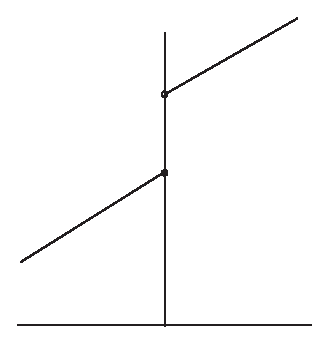
\includegraphics{PS/linear.eps}
  \caption{A piecewise linear function}
  \label{fig:discontinuous}
\end{figure}



We break the interval in two at $x=0$, forming two compact
intervals $[-1,0]$ and $[0,1]$.  We have continuous functions
$f_-:[-1,0]\to \R$ and $f_+:[0,1]$, such that
    $$
    f(x)=
    \begin{cases}
        f_-(x) & x\in[-1,0],\\
        f_+(x) & \text{otherwise}.
    \end{cases}
    $$
We have replaced the discontinuous function by a pair of
continuous functions on smaller intervals, at the expense of
duplicating the point of discontinuity $x=0$.  We view this pair
of functions as a single function $F$ on the compact topological
space with two components
    $$[-1,0]\times\{-\} \text{\ and\ } [0,1]\times\{+\}.$$
where $F(x,a) = f_a(x)$, and $a\in\{-,+\}$.

This is the approach that we follow in general with the Kepler
conjecture.  The function $\sigma$ is defined by a series of case
statements, and the function does not extend continuously across the
boundary of the cases.  However, in the degenerate cases that land
precisely between two or more cases, we form multiple copies of
decomposition star for each case, and place each case into a
separate compact domain on which the function $\sigma$ is
continuous.

This can be formalized as a {\it colored space}.  A colored space
is a topological space $X$ together with an equivalence relation
on $X$ with the property that no point $x$ is equivalent to any
other point in the same connected component as $x$.   We refer to
the connected components as colors, and call the points of $X$
{\it colored points}.  We call the set of equivalence classes of
$X$ the underlying uncolored space of $X$. Two colored points are
equal as uncolored points if they are equivalent under the
equivalence relation.
\index{colored!space}
\index{colored!points}

In our example, there are two colors ``$-$'' and ``$+$.''  The
equivalence class of $(x,a)$ is the set of pairs $(x,b)$ with the
same first coordinate.  Thus, if $x\ne0$, the equivalence class
contains one element $(x,\sign(x))$, and in the boundary case
$x=0$ there are two equivalent elements $(0,-)$ and $(0,+)$.

In our treatment of decomposition stars, there are various cases:
whether an edge has length less than or greater than $2t_0$, less
than or greater than $\sqrt8$, whether a face has circumradius
less than or greater than $\sqrt2$, and so forth. By duplicating
the degenerate cases (say an edge of exact length $2t_0$),
creating a separate connected component for each case, and
expressing the optimization problem on a colored space, we obtain
a continuous function $\sigma$ on a compact domain $X$.

The colorings have in general been suppressed in places from the
notation. To obtain consistent results, a statement about
$x\in[2,2t_0]$ should be interpreted as having an implicit
condition saying that $x$ has the coloring induced from the
coloring on the component containing $[2,2t_0]$.  A later
statement about $y\in[2t_0,\sqrt8]$ deals with $y$ of a different
color, and no relation between $x$ and $y$ of different colors is
assumed at the endpoint $2t_0$.




\shortversion{\chapter{Scoring~[Ferguson,~Hales]\index{Ferguson}}}
\longversion{\chapter{Scoring~[Ferguson,~Hales]\index{Ferguson}}}

\label{sec:scoring}

This \chap\  is coauthored by
Samuel P. Ferguson\index{Ferguson} and Thomas C. Hales.

In earlier \chaps, we describe each packing of unit balls by its set
$\Lambda\subset \ring{R}^3$ of centers of the packing.  We showed
that we may assume that our packings are saturated in the sense that
there is no room for additional balls to be inserted into the
packing without overlap. Lemma~\ref{lemma:deltabound} shows that the
Kepler conjecture follows if for each saturated packing $\Lambda$ we
can find a function $A:\Lambda\to\ring{R}$ with two properties: the
function is fcc-compatible and it is saturated in the sense of
Definition~\ref{def:negligible}.

The purpose of the first part of this \chap\ is to define a
function $A:\Lambda\to\ring{R}$ for every saturated packing
$\Lambda$ and to show that it is negligible.  The formula defining
$A$ consists of a term that is a correction between the volume of
the Voronoi cell $\Omega(v)$ and that of the $V$-cell $\op{VC}(v)$
and a further term coming from simplices of the $Q$-system that
have a vertex at $v$.

A major theorem in this \paper\ will be that this negligible
function is fcc-compatible.  The proof of fcc-compatibility can be
expressed as a difficult nonlinear optimization problem over the
compact topological space $\op{DS}$ that was introduced in
\Chap~\ref{sec:compact}.  In fact, we construct a continuous
function $A_0$ on the space $\op{DS}$ such that for each saturated
packing $\Lambda$ and each $v\in\Lambda$, the value of the function
$A$ at $v$ is a value in the range of the function $A_0$ on
$\op{DS}$. In this way, we are able to translate the
fcc-compatibility of $A$ into an extremal property of the function
$A_0$ on the space $\op{DS}$.

The proof of fcc-compatibility is more conveniently couched as an
optimization problem over a function that is related to the
function $A_0$ by an affine rescaling.   This new function is
called the score and is denoted $\sigma$.  (The exact relationship
between $A_0$ and $\sigma$ appears in Definition~\ref{def:score}.)
The function $\sigma$ is a continuous function on the space
$\op{DS}$. This function is defined in the final paragraphs of this
\chap.


\section{Definitions}
\label{sec:rules}


For every saturated packing $\Lambda$, and $v\in \Lambda$, there
is a canonically associated decomposition star $D(v,\Lambda)$. The
negligible function $A:\Lambda\to\ring{R}$ that we define is a
composite
  \begin{equation}
  A = A_0\circ D(\cdot,\Lambda)
  :\Lambda\to DS\to \ring{R},\quad v\mapsto D(v,\Lambda)\mapsto
  A_0(D(v,\Lambda)),
  \label{eqn:A}
  \end{equation}
where $A_0:\op{DS}\to\ring{R}$ is defined by
Equations~\ref{eqn:A1} and \ref{eqn:a1-sigma} below.  Each simplex
in the $Q$-system with a vertex at $v$ defines by translation to
the origin a simplex in the $Q$-system with a vertex at $0$
attached to $D(v,\Lambda)$. Let $\CalQ_0(D)$ be this set of
translated simplices at the origin. This set is determined by $D$.

\begin{definition} \label{def:context}
Let $Q$ be a quarter in $\CalQ_0(D)$.  We say that the {\it
context\/} of $Q$ is $\x(p,q)$ if there are $p$ anchors and $p-q$
quarters along the diagonal of $Q$. Write $c(Q,D)$ for the context
of $Q\in\CalQ_0(D)$.
\end{definition}\index{context (of a quarter)}

$q$ is the number of ``gaps'' between anchors around the diagonal.
For example, the context of a quarter in a quartered octahedron is
$\x(4,0)$.  The context of a single quarter is $\x(2,1)$.
%The
%only possible contexts of upright quarters in a quad cluster are
%$\x(4,0)$, $\x(3,1)$, and $\x(2,1)$. Of course, $Q$ and $\hat Q$
%have the same context. The definition of $\sigma(Q)$ depends on
%the context of $Q$.


The function $A_0$ will be defined to be
a continuous function on $\op{DS}$ of the
form
  \begin{equation}
  A_0(D) = -\op{vol}\,(\Omega(D)) + \op{vol}\,(\op{VC}(D)) +
   \sum_{Q\in\CalQ_0(D)} A_1(Q,c(Q,D),0).
   \label{eqn:A1}
   \end{equation}
Thus, the function $A_0$ measures the difference in volume between
the Voronoi cell and $V$-cell, as well as certain contributions
$A_1$ from the $Q$-system. The function $A_1(Q,c,v)$ depends on
$Q$, its context $c$, and a vertex $v$ of $Q$.  The function
$A_1(Q,c,v)$ will not depend on the second argument when $Q$ is a
quasi-regular tetrahedron.  (The context is not defined for such
simplices.)



\begin{definition} \label{def:rogers}
An {\it orthosimplex} consists of the convex hull of
$\{0,v_1,v_1+v_2,v_1+v_2+v_3\}$, where $v_2$ is a vector
orthogonal to $v_1$, and $v_3$ is orthogonal to both $v_1$ and
$v_2$.  We can specify an orthosimplex up to congruence by the
parameters $a = |v_1|$, $b=|v_1+v_2|$, and $c=|v_1+v_2+v_3|$,
where $a\le b\le c$. This parametrization of the orthosimplex
departs from the usual parametrization by the lengths $|v_1|$,
$|v_2|$, $|v_3|$. For $a\le b\le c$,  the {\it Rogers simplex\/}
$R(a,b,c)$ is an orthosimplex of the form
$$R(a,b,c)=S(a,b,c,\sqrt{c^2-b^2},\sqrt{c^2-a^2},\sqrt{b^2-a^2}).$$
See Figure~\ref{fig:rogers}.
%
 \index{Rogers simplex}
 \index{orthosimplex}
\end{definition}

\begin{figure}[htb]
  \centering
  \includegraphics{PS/rogers.eps}
  \caption{The Rogers simplex is an orthosimplex.}
  \label{fig:rogers}
\end{figure}

\begin{definition}\label{def:quoin}\index{quoin}
Let $R$ be a Rogers simplex.  We define the {\it quoin} of $R$ to
be the  wedge-like solid (a quoin) situated above $R$. It is
defined as the solid bounded by the four planes through the faces
of $R$ and a sphere of radius $c$ at the origin. (See
Figure~\ref{fig:quoin}.)   We let $\quo(R)$ be the volume of the
quoin over $R$.  \shortversion{An explicit formula appears in
\cite{KC}.}  \longversion{If $R=R(a,b,c)$ is a Rogers simplex, the
volume $\quo(R)$ is given explicitly as follows\index{Rogers
simplex}
    \begin{equation}
    \begin{array}{lll}
    6\quo(R) &= (a+2c)  %
    % -(a^2+ac-2c^2)
    (c-a)^2\arctan(e)
        +a(b^2-a^2)e\\&-4c^3\arctan(e(b-a)/(b+c)),
    \label{eqn:3.3}
    \end{array}
    \end{equation}
where $e\ge0$ is given by $e^2(b^2-a^2)=(c^2-b^2)$.}
%
 \index{quoin}
\end{definition}


\begin{figure}[htb]
  \centering
  \includegraphics{PS/quoin.eps}
  \caption{The quoin above a Rogers simplex is the part of the
  shaded solid outside
   the illustrated box.  It is bounded by the shaded planes, the plane through
   the front face of the box, and a sphere
   centered at the origin passing through the opposite corner of the box.}
  \label{fig:quoin}
\end{figure}

Let $S$ be a simplex and let $v$ be a vertex of that simplex. Let
$\op{VC}(S,v)$ be the subset of $|S|$ consisting of points closer
to $v$ than to any other vertex of $S$. By
Lemma~\ref{lemma:Q-divide}, if $S\in\CalQ_0(D)$, then
$$\op{VC}(S,0) = \op{VC}(D)\cap |S|.$$
Under the assumption that $S$ contains its circumcenter and that
every one of its faces contains its circumcenter, an explicit
formula for the volume $\op{vol}(\op{VC}(S,v))$ has been
calculated in \cite[Section~8.6.3]{part1}. This volume formula is
an algebraic function of the edge lengths of $S$, and may be
analytically continued to give a function of $S$ with chosen
vertex $v$:
  $$\op{vol}\,\op{VC}^\op{an}(S,v).$$

\begin{lemma}\label{lemma:cap-rogers}
Let $B(0,t)$ be a ball of radius $t$ centered at the origin.  Let
$v_1$ and $v_2$ be vertices.  Assume that $|v_1|< 2t$ and $|v_2|<2
t$.  Truncate the ball by cutting away the caps
   $$\op{cap}_i = \{x\in B(0,t) :  |x- v_i| < |x|\}.$$
Assume that the circumradius of the triangle $\{0,v_1,v_2\}$ is
less than $t$. Then the intersection of the caps $\op{cap}_1\cap
\op{cap}_2$ is the union of four quoins.
\end{lemma}

\begin{proof} This is true by inspection.  See Figure~\ref{fig:capriquoin}.
Slice the intersection $\op{cap}_1\cap\op{cap}_2$ into four pieces
by two perpendicular planes: the plane through $\{0,v_1,v_2\}$,
and the plane perpendicular to the first and passing through $0$
and the circumcenter of $\{0,v_1,v_2\}$.  Each of the four pieces
is a quoin.
\end{proof}

\begin{figure}[htb]
  \centering
  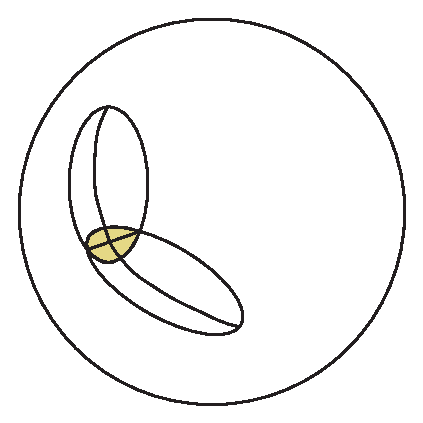
\includegraphics{PS/capriquoin.eps}
  \caption{The intersection of two caps on the unit ball can
   be partitioned into four quoins (shaded).}
  \label{fig:capriquoin}
\end{figure}

\begin{definition}\label{def:sol}
Let $v\in\ring{R}^3$ and let $X$ be a measurable subset of
$\ring{R}^3$. Let $\sol(X,v)$ be the area of the radial projection
of $X\setminus\{0\}$ to the unit sphere centered at the origin. We
call this area the {\it solid angle\/} of $X$ (at $v$).  When
$v=0$, we write the function as $\sol(X)$.
 %
 \index{sol}
 \index{solid angle}
\end{definition}


Let $S=\{v_0,v_1,v_2,v_3\}$ be a simplex. Fix $t$ in the range
$t_0\le t\le\sqrt2$.  Assume that $t$ is at most the circumradius
of $S$. Assume that it is at least the circumradius of each of the
faces of $S$.  Let $\op{VC}_t(S,v_0)$ be the intersection of
$\op{VC}(S,v_0)$ with the ball $B(v_0,t)$. Under the assumption
that $S$ contains its circumcenter and that every one of its faces
contains it circumcenter, an explicit formula for the volume
$$\op{vol}(\op{VC}_t(S,v_0))$$ is calculated by means of
Lemma~\ref{lemma:cap-rogers} through a process of inclusion and
exclusion. In detail, start with $|S|\cap B(v_0,t)$. Truncate this
solid by caps $\op{cap}_1$, $\op{cap}_2$,\index{cap} and
$\op{cap}_3$ bounded by the sphere of radius $t$ centered at $v_0$
and the perpendicular bisectors (respectively) of $\{v_0,v_1\}$,
$\{v_0,v_1\}$, $\{v_0,v_2\}$.  If we subtract the volume of each
cap $\op{cap}_i$, then we must add back the volume of the doubly
counted intersections of the caps.  The intersections of caps are
given as quoins (Lemma~\ref{lemma:cap-rogers}).  This leads to the
following formula. Let $h_i = |v_i|/2$ and
$\eta_{ij}=\eta(0,v_i,v_j)$, and let $S_3$ be the group of
permutations of $\{1,2,3\}$ in
\begin{equation}
   \op{vol}\,\op{VC}_t(S,v_0) =
   \sol(S)/3 - \sum_{i=1}^3 \frac{\dih(S,v_i)}{2\pi}\op{vol}\,\op{cap_i}
   +\sum_{(i,j,k)\in S_3} \quo(R(h_i,\eta_{ij},t)).
   \label{eqn:vol-theta-0}
\end{equation}


We extend Formula~\ref{eqn:vol-theta-0} by setting
    $$\quo(R(a,b,c)) = 0,$$
if the constraint $a < b < c$ fails to hold.  Similarly, set
$\op{vol}\,\op{cap}_i=0$ if $|v_i|\ge 2t$.  With these
conventions,  Formula~\ref{eqn:vol-theta-0} extends to all
simplices.  We write the extension of $\op{vol}\,\op{VC}_t(S,v)$
as
$$\op{vol}\,{\op{VC}^+_t}(S,v).$$



\begin{definition}\label{def:svor}
   Let\footnote{In the paper \cite{spp}, the volumes in this definition were
   volumes of Voronoi cells, and hence the notation $\vor$ for the function was
adopted. We retain $\vor$ in the notation, although this direct
connection with Voronoi cells has been lost.}
      $$
      \svor(S,v) = 4(-\doct \op{vol}\,\op{VC}^{\op{an}}(S,v)
         +\sol(S,v)/3),$$
      $$
      \svor(S,v,t) = 4(-\doct \op{vol}\,\op{VC}^+_{t}(S,v)
         +\sol(S,v)/3),$$
   and
      $$
      \svor_0(S,v) = \svor(S,v,t_0).
      $$
   When it is clear from the context that the vertex $v$ is
   fixed at the origin, we drop $v$ from the notation of these
   functions.
   If $S=\{v_1,v_2,v_3,v_4\}$, we define $\Gamma(S)$ as the average
   \begin{equation}
   \Gamma(S) = \frac{1}{4}\sum_{i=1}^4\svor(S,v_i).
   \label{eqn:gamma}
   \end{equation}
   The average $\Gamma(S)$ is called the {\it compression} of $S$.
%
 \index{compression}
 \index{ZZcamma@$\Gamma$}
\end{definition}

\begin{definition}
Let $Q$ be a quarter.   Let $\eta^+(Q)$ be the maximum of the
circumradii of the two faces of $Q$ along the diagonal of $Q$.
\end{definition}

Let $Q$ be a simplex in the $Q$-system.  We define an involution
$v\to \hat v$ on the vertices of $Q$ as follows.  If $Q$ is a
quarter and $v$ is an endpoint of the diagonal, then let $\hat v$
be the opposite endpoint of the diagonal.  In all other cases, set
$\hat v = v$.

We are ready to complete the definition of the function
$A:\Lambda\to\ring{R}$.  The definition of $A$ was reduced to that
of $A_0$ in Equation~\ref{eqn:A}.  The function $A_0$ was reduced
in turn to that of $A_1$ in Equation~\ref{eqn:A1}. To complete the
definition, we define $A_1$.

\begin{definition}\label{def:sigma}
Set
   \begin{equation}\label{eqn:a1-sigma}
   A_1(S,c,v) = -\op{vol}\,\op{VC}(S,v)+
      \frac{\sol(S,v)}{3\doct} - \frac{\sigma(S,c,v)}{4\doct}.
      \end{equation}  where $\sigma$ is given as follows:
      %
      \index{AZ1@$A_1$}
      \index{ZZsigma@$\sigma$}
\begin{enumerate}
\item If $S$ is a quasi-regular tetrahedron:
   \begin{enumerate}
      \item If the circumradius of $S$ less than $1.41$, set
         $$\sigma(S,-,v)=\Gamma(S)$$
      \item If the circumradius of $S$ is at least $1.41$, set
         $$\sigma(S,-,v)=\svor(S,v).$$
   \end{enumerate}
\item If $S$ is a strict quarter:
   \begin{enumerate}
      \item If $\eta^+(S) <\sqrt2$:
         \begin{enumerate}
         \item If the context $c$ is $(2,1)$ or $(4,0)$, set
                  $$\sigma(S,c,v)=\Gamma(S)$$
         \item If the context of $S$ is anything else, set
                  $$\sigma(S,c,v)=\Gamma(S) +
                     \frac{\svor_0(S,v)-\svor_0(S,\hat v)}{2}.$$
         \end{enumerate}
      \item If $\eta^+(S) \ge\sqrt2$:
         \begin{enumerate}
         \item If the context of $S$ is $(2,1)$, set
                  $$\sigma(S,c,v)=\svor(S,v).$$
         \item If the context of $S$ is $(4,0)$, set
                  $$\sigma(S,c,v)=\frac{\svor(S,v)+\svor(S,\hat v)}{2}.$$
         \item If the context of $S$ is anything else, set
                  $$\sigma(S,c,v)=\frac{\svor(S,v)+\svor(S,\hat
                  v)}{2}
                     +\frac{\svor_0(S,v)-\svor_0(S,\hat v)}{2}.$$
         \end{enumerate}
   \end{enumerate}
\end{enumerate}
When the context and vertex $v$ are given, we often write
$\sigma(S)$ or $\sigma(S,v)$ for $\sigma(S,c,v)$.

When $\eta^+<\sqrt2$, we say that the quarter has compression type.
Otherwise, we say it has Voronoi type.  To say that a quarter has
compression type means that $\Gamma(S)$ is one term of the function
$\sigma(S,v)$. It does not mean that $\Gamma(S)$ is equal to
$\sigma(S,v)$.
%
 \index{Voronoi type}
 \index{compression type}
\end{definition}

\longversion{The definition of $\sigma$ on quarters can be expressed
a second way in terms of a function $\mu$.  If $S$ is a quarter, set
    \begin{equation}
    \mu(S,v)=\begin{cases}
    \Gamma(S),&  \text{ if }\eta^+(S)<\sqr2,\\
    \svor(S,v),& \hbox{otherwise.}\end{cases}
    \label{eqn:3.8}
    \end{equation}
If $S$ is a flat quarter, we have $\sigma(S,c,v)=\mu(S,v)$, for all
contexts $c$.}

\longversion{Suppose $S$ is an upright
quarter.\index{quarter!upright} Definition~\ref{def:sigma} can be
expressed as follows.}

\longversion{
\begin{itemize}
 \item context $\x(2,1)$:  Set $\sigma(S,c,v)=\mu(S,v)$.
 \item context
    $\x(4,0)$:  Set $\sigma(S,c,v)=(\mu(S,v)+\mu(S,\hat v))/2$.
 \item other contexts:
 Set $\sigma(S,c,v)=(\mu(S,v)+\mu(S,\hat v)+ \svor_0(S,v) - \svor_0(S,\hat v))/2$.
\end{itemize}
 }


\begin{lemma}  $A_0:\op{DS}\to\ring{R}$ is continuous.
\end{lemma}

\begin{proof}
The continuity of $D\mapsto\op{vol}\,\op{VC}(D)$ is proved in
Lemma~\ref{lemma:vc-cont}.  The continuity of
$D\mapsto\op{vol}\,\Omega(D)$ is similarly proved.  The terms
$\op{vol}\,\op{VC}(S,v)$ and $\sol(S,v)$ are continuous. To complete
the proof we check that the function $\sigma(S,c,v)$ is continuous.
It is not continuous when viewed as a function of the set of
quarters, because of the various cases breaking at circumradius
$1.41$ and $\eta^+(S)=\sqrt2$.  However, these cutoffs have been
inserted into the data defining a decomposition star (in the
indexing sets $I_8$ and $I_9$).  Thus, the different cases in the
definition of $\sigma(S,c,v)$ land in different connected components
of the space $\op{DS}$ and continuity is obtained.
\end{proof}

We conclude this section with a result that will be of use in the
next section.

\begin{lemma}\label{lemma:A1-cancel}
Let $S=\{v_1,v_2,v_3,v_4\}$ be a simplex in the $S$-system,  and $c$
its context.   Then
   $$\sum_{i=1}^4 A_1(S,c,v_i)=0.$$
\end{lemma}

\begin{proof}
   By Formula~\ref{eqn:a1-sigma}, this is equivalent to
      \begin{equation}
      \sum_{i=1}^4 \sigma(S,c,v_i) = \sum_{i=1}^4
      \svor(S,c,v_i).
      \label{eqn:sigma-4}
      \end{equation}
Equation~\ref{eqn:sigma-4} is evident from
Definition~\ref{def:sigma} for $\sigma$.  In fact, the terms of the
form $\svor_0$ have opposing signs and cancel when we sum. The other
terms are weighted averages of the terms $\svor(S,c,v_i)$.
Equation~\ref{eqn:sigma-4} is thus established by noting that a sum
is unaffected by taking weighted averages of its terms.
\end{proof}


\section{Negligibility} \label{sec:negligible}

Let $B(x,r)$ be the closed ball of radius $r\in\ring{R}$ centered
at $x$.  Let $\Lambda(x,r)=\Lambda\cap B(x,r)$.

Recall from Definition~\ref{def:negligible} that a function
$A:\Lambda\to\ring{R}$ is said to be {\it negligible} if there is
a constant $C_1$ such that for all $r\ge1$, we have
   $$\sum_{v\in\Lambda(x,r) } A(v) \le C_1 r^2.$$
%
 \index{negligible}


Recall that a function $A: \Lambda\to\ring{R}$ given by
Equation~\ref{eqn:A}.  Explicitly, let
   $$A(v) = A_0(D(v,\Lambda)),$$
where $A_0$ in turn depends on functions $A_1$ and $\sigma$, as
determined by Equations~\ref{eqn:A1} and \ref{eqn:a1-sigma}, and
Definition~\ref{def:sigma}.

\begin{theorem}\label{lemma:negligible}
The function $A$ of Equation~\ref{eqn:A} is negligible.
\end{theorem}

\begin{proof} First we consider a simplification, where we replace
   $A$ with $A'$ defined by
      $$
      A'(v,\Lambda) = -\op{vol}(\Omega(D(v,\Lambda)))+
         \op{vol}(\op{VC}(D(v,\Lambda))).$$
(That is, at first we ignore the function $A_1$.) The Voronoi
cells partition $\ring{R}^3$, as do the $V$-cells.  We have
$\Omega(v,\Lambda)\subset B(v,2)$ (by saturation) and
$\op{VC}(v,\Lambda)\subset B(v,2\sqrt3)$ (by
Definition~\ref{def:phi}). Hence the Voronoi cells with $v\in
\Lambda(x,r)$ cover $B(x,r-2)$. Moreover, the $V$-cells with $v\in
\Lambda(x,r)$ are contained in $B(x,r+2\sqrt3)$.  Hence
   $$
   \sum_{v\in\Lambda(x,r)} A'(v) \le -\op{vol}\,B(x,r-2)
      +\op{vol}\,B(x,r+2\sqrt3)\le C_1' r^2
   $$
for some constant $C_1'$.

If we do not make the simplification, we must also include the sum
   $$\sum_{v\in\Lambda(x,r)} \sum_{Q\in\CalQ_v(D(v,\Lambda))}
      A_1 (Q,c,v).$$
Each quarter $Q=\{v_1,v_2,v_3,v_4\}$ in the $Q$-system occurs in
four sets $\CalQ_{v_i}(D(v_i,\Lambda))$.  By
Lemma~\ref{lemma:A1-cancel} the sum cancels, except when some
vertex of $Q$ lies inside $\Lambda(x,r)$ and another lies outside.
Each such simplex lies inside a shell of width $2\sqrt8$ around
the boundary.  The contribution of such boundary terms is again
bounded by a constant times $r^2$.  This completes the proof.
\end{proof}


\section{Fcc-compatibility}

We have constructed a negligible function $A$.  The rest of this
\paper\ will prove that this function is fcc-compatible.   This
section translates fcc-compatibility into a property that will be
easier to prove.  To begin with, we introduce a rescaled version
of the function $A$.

\begin{definition}\label{def:score}
Let $\sigma:\op{DS}\to\ring{R}$ be given by
   $$\sigma(D) = -4\doct (\op{vol}\,\Omega(D) + A_0(D)) +
   16\pi/3.$$
It is called the {\it score} of the decomposition star.
%
 \index{score}
 \index{ZZsigma@$\sigma(D)$}
\end{definition}

Recall from Definition~\ref{def:pt} the constant $\pt\approx
0.05537$.  This constant is called a point.\index{point}

\begin{lemma}\label{lemma:8pt-compat}
Let $A_0$, $A$, and $\sigma$ be the functions defined by
Equations~\ref{eqn:A}, \ref{eqn:A1}  \ref{eqn:a1-sigma}, and
Definition~\ref{def:sigma}. The following are equivalent.
\begin{enumerate}
  \item The minimum of the function on $\op{DS}$ given by
      $$D\mapsto \op{vol}\,\Omega(D) + A_0(D)$$
is $\sqrt{32}$.
  \item The maximum of $\sigma$ on $\op{DS}$ is $8\,\pt$.
\end{enumerate}
Moreover, these statements imply
\begin{itemize}
  \item For every saturated packing $\Lambda$,
  the function $A$ is
  fcc-compatible.
\end{itemize}
\end{lemma}

(Eventually, we prove fcc-compatibility by proving
$\sigma(D)\le8\,\pt$ for all $D\in\op{DS}$.)

\begin{proof} To see the equivalence of the first and second statements,
use Definition~\ref{def:score},  and the identity
   $$8\,\pt = -4\doct (\sqrt{32}) + 16 \pi/3.$$
(Note that this identity is parallel in form with
Definition~\ref{def:score} for $\sigma$.)

For a given saturated packing $\Lambda$, the function $A$ has the
form $A(v) = A_0(D(v,\Lambda))$.  Also, $\Omega(D(v,\Lambda))$ is
a translate of $\Omega(v)$, the Voronoi cell at $v$.  In
particular, they have the same volume.  Thus,
$\op{vol}\,\Omega(v)+A(v)$ lies in the range of the function
   $$\op{vol}\,\Omega(D) + A_0(D)$$
on $\op{DS}$.  The minimum of this function is $\sqrt{32}$ by the
first of the equivalent statements.  It now follows from the
definition of fcc-compatibility, that $A:\Lambda\to\ring{R}$ is
indeed fcc-compatible.
\end{proof}

\begin{theorem}\label{lemma:exista}
If the maximum of the function $\sigma$ on
$\op{DS}$ is $8\,\pt$, then for every saturated packing $\Lambda$
there exists a negligible fcc-compatible function $A$.
\end{theorem}

\begin{proof} This follows immediately from Theorem~\ref{lemma:negligible}
and Lemma~\ref{lemma:8pt-compat}.
\end{proof}



\section{Scores of Standard Clusters}
\label{sec:ssc}

The last section introduced a function $\sigma$ called the score. We
show that the function $\sigma$ can be expressed as a sum over terms
attached to each of the standard regions.

\begin{definition} \label{def:standard-cluster}
A {\it standard cluster\/} is a pair $(R,D)$ where $D$ is a
decomposition star and $R$ is one of its standard regions.  A {\it
quad cluster\/} is the standard cluster obtained when the standard
region is a quadrilateral.
\end{definition}
%
 \index{cluster!standard}
 \index{cluster!quad}
 \index{quad cluster}

%Recall $|S|$ is the convex hull of a set $S\subset
%\ring{R}^3$.

We break $\sigma$ into a sum
   \begin{equation}
   \sigma(D) = \sum_R\,\sigma_R(D),
   \end{equation}
indexed by the standard clusters $(R,D)$.  Let
   $$
   \op{VC}_R(D) = \op{VC}(D)\cap \op{cone}(R),
   $$
whenever $R$ is a measurable subset of the unit sphere.  Let
   $$
   \CalQ_0(R,D) = \{Q\in \CalQ_0(D) : Q\subset \op{cone}(R)\}.
   $$
By Lemma~\ref{lemma:Q-in-region},
 each $Q$ is entirely contained in the cone over a single
standard region.

\begin{definition} \label{def:score-std-region}
   Let $R$ be a measurable subset of the unit sphere.  Set
      $$
      \vor_R(D) =4\left(-\doct \op{vol}\,\op{VC}_R(D)  + \sol(R)/3\right)
      $$
      Let $R$ be a standard region. Set
      $$
      \sigma_R(D) = \vor_R(D) - 4\doct
         \sum_{Q\in\CalQ_0(R,D)} A_1(Q,c(Q,D),0).
      $$
\index{vzorR@$\vor_R$} \index{zzsigmaR@$\sigma_R$}
\end{definition}

\begin{lemma} $\sigma(D) = \sum_R\sigma_R(D)$, where the sum runs
over all standard regions $R$.
\end{lemma}

\begin{proof}
   $$
   \begin{array}{lll}
      \sigma(D)
      &= -4\doct (\op{vol}\,\Omega(D) + A_0(D))+16\pi/3\\
      &= -4\doct (\op{vol}\,\op{VC}(D)+\sum_{Q\in\CalQ_0(D)}
         A_1(Q,c(Q,D),0)) + (4) (4\pi/3)\\
      &= \sum_R 4\left (-\doct \op{vol}\,\op{VC}_R(D) -\doct
         \sum_{Q\in\CalQ_0(R,D)} A_1(Q,c(Q,D),0) +
         \sol(R)/3\right).
   \end{array}
   $$
\end{proof}

\longversion{
Also, we have
    \begin{equation}
    \op{vor}(D)=\sum_{R\in \CalR(D)}
    \op{vor}_R(D).
    \label{eqn:vorD}
    \end{equation}
    }

\begin{lemma}\label{lemma:R'}
Let $R'\subset R$ be the part of a standard region that does not
lie in any cone over any $Q\in Q_0(R,D)$.  Then
   $$
   \sigma_R(D) = \vor_{R'}(D)
      + \sum_{Q\in\CalQ_0(R,D)} \sigma(Q,c(Q,D),0).
   $$
\end{lemma}

\begin{proof} Substitute the definition of $A_1$
(Equation~\ref{eqn:a1-sigma}) into the definition of
$\sigma_R(D)$, noting that $\op{VC}(Q,0) = \op{VC}_{R''}(D)$,
where $R''$ is the intersection of $Q$ with the unit sphere.
\end{proof}

\begin{remark}   Lemma~\ref{lemma:R'} explains why we have chosen
the same symbol $\sigma$ for the functions $\sigma_R(D)$ and
$\sigma(Q,c,v)$.  We can view Lemma~\ref{lemma:R'} as asserting a
linear relation in the functions $\sigma$:
   $$\sigma_R(D) = \sigma_{R'}(D) + \sum \sigma(Q,c,0).$$
The sum runs over $Q\in\CalQ_0$ that lie in the cone over $R$.
\end{remark}

\longversion{\section{Scores of Simplices and Cones}}

\longversion{Many of the functions in this paper are defined by
terms involving volumes of simple solids.  To give estimates on the
functions, it is often convenient to partition the solids into
smaller pieces and then define corresponding functions on each of
the pieces.  For this reason, we define some variants of the
functions $\vor$ and $\sigma$.}

\longversion{
\begin{remark}\label{remark:vor}\index{vor}\index{c-vor}\index{score}
We now define a few more variants of the function $\vor$. The
function $\svor$ and its truncated version  $\svor(\cdot,t)$ have
been defined already. The function $\vor_R(D)$ will also be given a
truncated version $\vor_R(D,t)$, for a real truncation parameter
$t\ge 0$. The special case, $\vor_R(D,t_0)$ will be abbreviated
$\vor_{0,R}(D)$. There will be another variant $\op{r-vor}$ for
Rogers simplices, and another $\op{c-vor}$ for general sets.  The
general form of these functions is
    $$\op{c-vor}(X) = 4 (-\doct\op{vol}(X) + \sol(X)/3),$$
for any subset $X\subset \ring{R}^3$.   The differences between the
different versions of $\vor$ come from the different choices of the
set $X$ and the way they are parameterized.
\end{remark}}

\longversion{
\begin{definition}  \label{def:r-vor}\index{r-vor}
Let $R=R(a,b,c)$ be a Rogers simplex. Assume that the
vertex terminating the edges of lengths $a$, $b$, and $c$ is
situated at the origin. Let
    $$\op{r-vor}(R) = 4 (-\doct\op{vol}(R) + \sol(R)/3).$$
\end{definition}}


% \index{Voronoi function} We define the simplex
%version $\svor$ of the function as follows. We begin with its
%definition for simplices $S$ whose faces have positive
%orientation. Assume that $S$ has a distinguished vertex $v$, which
%e fix at the origin. Let $\sol(S)$ be the solid angle of $S$ at
%its distinguished vertex.\index{sol} Set
%$\doct=(\pi-4\arctan(\sqr2/5))/\sqr8$. Set
%    \begin{equation}
%   \svor(S) = 4(-\doct \op{vol}(\op{VC}(S,0)) + \sol(S)/3),
%   \label{eqn:3.1}
%    \end{equation}
%This formula may be analytically continued to simplices $S$ with
%negatively oriented faces, and $\svor(S)$ is defined in general by
%this analytic continuation. A formula for $\svor$ is found in
%\cite[Sec. 8.6]{part1}.  Let $S_1,\ldots, S_4$ be equal to $S$
%as unlabeled simplices, but with different distinguished vertices.

\longversion{
\begin{definition}\label{def:cone}
 Let $C(h,t)$ denote the compact cone of height $h$
and circular base. Set
%of area $\pi(t^2-h^2)$. Set
    $$
    \phi(h,t)=2(2-\doct  t h (h+t))/3.
    $$
\index{right circular cone}\index{cone}
 Then
    \begin{equation}
    \op{c-vor}(C(h,t))=2\pi(1-h/t)\phi(h,t).
    \label{eqn:3.2}
    \end{equation}
 \end{definition}
    }

\longversion{
\begin{remark}\label{remark:score}
Below, we introduce variants of the function $\sigma$. We have
already encountered $\sigma$ in Definitions~\ref{def:sigma},
\ref{def:score}, and \ref{def:score-std-region}. Informally, we call
$\sigma$ (and various functions that are closely related to it) the
{\it score}. Equation~\ref{eqn:3.2} represents the {\it score\/} of
$C(h,t)$. The solid angle of $C(h,t)$ is $2\pi(1-h/t)$, so
$\phi(h,t)$ is the score per unit area. Also, $\phi(t,t)$ is the
score per unit area of a ball of radius $t$. That is, $\phi(t,t) =
4(-\doct\op{vol}/\sol + 1/3)$.\index{score}
\end{remark}
}


\longversion{ We set
    \begin{equation}
    \begin{array}{lll}
    \svor(S,t) &=
    \sol(S)\phi(t,t)
    +\sum_{i=1,\ h_i\le t}^3 d_i (1-h_i/t) (\phi(h_i,t)-
    \phi(t,t)) \\
    &-\sum_{(i,j,k)\in S_3}
    4\doct
    \quo(R(h_i,\eta(y_i,y_j,y_{k+3}),t)).
    \label{eqn:3.5}
    \end{array}
    \end{equation}
In the definition, we adopt the convention that $\quo(R)=0$, if
$R=R(a,b,c)$ does not exist (that is, if the condition
    $0< a\le b\le c$
is violated). In the second sum, $S_3$ is the set of permutations on
three letters. This definition is compatible with
Definition~\ref{def:svor}.}


%This formula has a simple geometric interpretation when the
%circumradius of $S$ is greater than $t$ and the circumradius of
%each face is less than $t$. It represents the score\index{score}
%of the part of the Voronoi cell at the origin that lies inside $S$
%and inside a ball of radius $t$.  This can be seen geometrically
%from Figure~\ref{fig:diag36}, which depicts the intersection of
%$S$ with the Voronoi cell as three quadrilaterals forming a
%triangle. The truncation in the second frame is shown as a shaded
%region. The truncated volume can be decomposed into a solid angle
%term, three conic terms, and six quoins (with appropriate sign
%conventions).  Hence the formula for $\svor(S,t)$. }



\longversion{ Similarly, we define $\vor_P(D,t)$ for arbitrary
standard clusters $(P,D)$.  (We shift notation from $R$ to $P$ for a
standard region to avoid conflict with Rogers simplices $R$ in the
following definition.)  Extending the notation in an obvious way, we
have
    \begin{equation}
    \begin{array}{lll}
    \vor_P(D,t) &=
    \sol(P)\phi(t,t)
    +\sum_{|v_i|\le 2t} d_i (1-|v_i|/(2t)) (\phi(|v_i|/2,t)-
    \phi(t,t)) \\
    &-\sum_{R} 4\doct \quo(R).
    \label{eqn:3.7}
    \end{array}
    \end{equation}
The first sum runs over vertices in $P$ of height at most $2t$. The
second sum runs over Rogers simplices $R(|v_i|/2,\eta(F),t)$ in $P$,
where $F=\{0,v_1,v_2\}$ is a face of circumradius $\eta(F)$ at most
$t$, formed by vertices in $P$.  The constant $d_i$ is the total
dihedral angle along $\{0,v_i\}$ of the standard cluster. The
truncations $t=t_0=1.255$ and $t=\sqr2$ will be of particular
importance.
    Set $A(h) = (1-h/t_0) (\phi(h,t_0)-\phi(t_0,t_0))$.\index{A}}

\longversion{
\begin{remark}  We have introduced both untruncated and truncated
versions of functions $\vor$ and $\sigma$.  The truncated versions
are used to give upper bounds on the untruncated versions.  For
example,  in the function $\sigma(D)$, the $V$-cell contributes
through its volume, as in Remark~\ref{remark:vor}.  The volume
appears with a negative coefficient $-4\doct$.  Thus, we obtain an
upper bound on $\sigma(D)$ by discarding bits of volume from the
$V$-cell.   This suggests that we might try to give upper bounds on
the score $\sigma(D)$ by truncating the $V$-cell in various ways.
This is the reason for the truncated versions of these functions.
\end{remark}}

\longversion{\section{The Example of a Dodecahedron}}

\longversion{
\begin{example}  The following example illustrates why better bounds
on the density of packings can be obtained with $\sigma(D)$ than
with a naive approach based on the volume of Voronoi cells.  By
scoring quasi-regular tetrahedra with the compression function
$\Gamma(S)$ rather than $\op{s-vor}(S)$, we will find that the score
is lowered below $8\,\pt$ for configurations with many quasi-regular
tetrahedra. To work one example, let us assume that the
decomposition star consists of $12$ vertices located at distance $2$
from the origin, at the vertices of a regular icosahedron. The score
is approximately
   $$20\,\Gamma(S(2,2,2,2.1092,2.1092,2.1092) \approx 1.8\,\pt < 8\,\pt.$$
If $\op{s-vor}(S)$ had been used, the score would violate Theorem
1.7:
   $$20\,\op{s-vor}(S) \approx 13.5493\,\pt > 8\,\pt.$$
(This is tied to the fact that the regular dodecahedron of
inradius $1$ has smaller volume than the rhombic dodecahedron of
inradius $1$.)
\end{example}
}

    \chapter{Geometric Detail}%DCG "The S-System" Sec.9, p85
    \label{sec:fine}
    \oldlabel{2}

The previous chapter gives  constructions unaided
needed to describe the top-level proof.  
Those constructions do not take us far.   This
chapter gives details needed to carry the proof to completion. 
We have discussed many of these constructions before, such
as V-cells, the Q-system, fans, and fitted crowns.  In this
chapter we look at how these structures are interrelated.

The top-level proof calls for
lower bounds on the volume of a $V$-cell.  
The strategy is to dissect the $V$-cell into small disjoint
pieces, each with an easily computed volume.  The volume
bound comes by adding these separate pieces of volume.
This chapter describes these pieces and shows that
they are disjoint subsets of the $V$-cell.  The next chapter
begins to add the contributions together.

If two pieces of the dissection lie in different connected components of
the complement of a fan, then they are disjoint.  This, in fact,
gives a useful way to  prove that pieces are disjoint. 

\section{Interaction}


%Let $\CalQ=\CalQ(\Lambda)$ be the $Q$-system.  
%For $v\in\Lambda$, let $\CalQ(\Lambda,v)$ be the subset
%of those with a vertex at $v$.\index{Index}{Qv@$\CalQ(\Lambda,v)$}
%% Defined already. def:q-system.


The exact volume of a general $V$-cell is never calculated.  
Lower bounds suffice.  L. Fejes T\'oth esimated
the volume of a Voronoi cells by intersecting it with a ball
$B(v_0,t)$ of some radius $t$.  This intersection is the
{\it truncated} Voronoi cell.  Truncation  also works for $V$-cells.
Often the truncated $V$-cell turns out to be almost identical to the
truncated Voronoi cell, which is much easier to estimate.
The chapter begins with some lemmas that compare the truncated $V$-cell with
the truncated Voronoi cell.


\begin{lemma} \tlabel{lemma:voronoi-truncation-over-Q}\rating{100}
Let $(\Lambda,v_0)$ be a centered packing.  Let $Z$ be the union
of the sets $\op{aff}_+(v_0,\{v_1,v_2\})$ as $\{v_0,v_1,v_2\}$
runs over the barriers with a vertex at $v_0$.  Let $X$ be the
union of the following tips:
   $$
   \op{aff}_+^0(v_0,\{v_1,v_2,v_3\}) \cap \op{aff}_-
   (\{v_1,v_2,v_3\},v_0)\cap \Omega_2(\Lambda,v_0).
   $$
as $\{v_0,v_1,v_2,v_3\}$ ranges over $\CalQ(\Lambda,v_0)$.
Then 
$$\Omega_2(\Lambda,v_0)
 \subset Z\cup X\cup \op{VC}(\Lambda,v_0).$$
%If $x$ lies in the \index{Index}{Voronoi cell} Voronoi cell at $v_0$, 
%but not in the $V$-cell at $v_0$, then there exists a
%simplex $Q\in\CalQ(\Lambda,v_0)$, such that $x$ lies in the cone (at $v_0$)
%over $Q$. Moreover, $x$ does not lie in  $\op{conv}^0(Q)$.
(That is, up to the null set $Z$, the $V$-cell contains
the truncated tip-reduced Voronoi cell.)
\end{lemma}

\begin{proof}  Let 
 $$x \in \Omega_2(\Lambda,v_0)
 \setminus (Z\cup\op{VC}(\Lambda,v_0)).
 $$
By
the definition of $V$-cell, there is a barrier $\{v_1,v_2,v_3\}$
such that
  $$\op{conv}\{v_1,v_2,v_3\}\cap \op{conv}^0\{v_0,x\}\ne\emptyset.$$ 
We have $v_0\not\in\{v_1,v_2,v_3\}$, for otherwise $x\in Z$, 
which is contrary to assumption. 
By tarski\tarf{tarski:vor-bar-tet}\tarf{tarski:vor-bar-quad},
the simplex $Q=\{v_0,v_1,v_2,v_3\}$ is a quasi-regular tetrahedron
or a flat quarter.  If the barrier is the face of a flat quarter,
then $Q$ too is in
the $Q$-system.  By tarski\tarf{tarski:pass-cone},  $x\in\op{aff}_+(v_0,\{v_1,v_2,v_3\})$.  
We get $x\in\op{aff}_+^0(v_0,\{v_1,v_2,v_3\})$ from $x\not\in Z$.

We have $x\in\op{aff}_-
   (\{v_1,v_2,v_3\},v_0)$. Otherwise, $\op{conv}^0\{v_0,x\}$ does
not meet $\op{conv}\{v_1,v_2,v_3\}$.
%We have $x\in\op{conv}(Q)\setminus Z$. Otherwise, 
%the barrier contains $x$, and the plane through the barrier contains
%$v_0$, so that $\{v_0,v_1,v_2,v_3\}$ is planar.  This is contrary
%to tarski\tarf{tarski:flat-Q}. 
The rest is clear.
\end{proof}

Although different estimates require different
truncation parameters, the truncation parameter $t_0$ that appears in
the next lemma is the most widely used.  A smaller truncation parameter never
appears.  A larger parameter is used only when the parameter $t_0$
has been tried and found wanting.  With tight truncation at $t_0$,
 the $V$-cell and Voronoi cell become
indistinguishable.

\begin{lemma}\tlabel{lemma:VC-Omega}\rating{100}
Let $(\Lambda,v_0)$ be a centered packing.
Inside the ball of radius $t_0$ at $v_0$, the $V$-cell and
Voronoi cell coincide up to a null set:
   $$B(v_0,t_0)\cap \op{VC}(\Lambda,v_0) \equiv B(v_0,t_0)\cap \Omega(\Lambda,v_0).$$
\end{lemma}

\begin{proof} Let $Z$ be the (finite) union of planes equidistant from $v_0$ and $w\in \Lambda(v_0,2t_0)$.  $Z$ is a null set.  Let $Y$ be the (finite) union of $\op{aff}_+(w,\{w_1,w_2\})$, for $w\in \Lambda(v_0,2t_0)$ and $\{w,w_1,w_2\}$ a barrier.  $Y$ is a null set.
The Voronoi cells $\Omega(\Lambda,w)$, $w\in\Lambda(v_0,2t_0)$ cover
$B(v_0,t_0)$ except for the null set $Z$.  
Suppose that some point  $x\not\in Z\cup Y$
lies in $$(B(v_0,\Lambda)\cap\op{VC}(\Lambda,v_0) )\setminus \Omega(\Lambda,v_0).$$
Then $x\in \Omega(\Lambda,w)$, where
$w\ne v_0$.  
% By Lemma~\ref{tarski:unobstr-t0}, 
From $x\not\in Y$, it follows that the point $v_0$ is
unobstructed  at $x$ by tarski\tarf{tarski:unobstr-t0}.  
Thus, $|x-w|< |x-v_0|\le t_0$.  By
tarski\tarf{tarski:unobstr-t0} again, $w$ is unobstructed at $x$, so
that $x\in \op{VC}(\Lambda,w)$, contrary to the assumption
$x\in\op{VC}(\Lambda,v_0)$.  Thus $B(v,t_0)\cap\op{VC}(\Lambda,v_0)\subset\Omega(\Lambda,v_0)$.

Similarly, if $x\in B(v_0,t_0)\cap \Omega(\Lambda,v_0)$ and $x\not\in Y$,
then $x$ is
unobstructed at $v_0$, and $x\in \op{VC}(\Lambda,v_0)$.
\end{proof}

\bigskip

%\begin{remark} The next lemma helps to determine which $V$-cell
%a given point $x$ belongs to.  If $x$ lies in the open cone over a
%simplex $Q_0$ in $\CalQ$, then Lemma~\ref{lemma:Q-divide}
%describes the $V$-cell decomposition inside $Q$;  beyond $Q$ the
%point $v_0$ is obstructed by a face of $Q$, so that such $x$ do not lie
%in the $V$-cell at $v_0$. 
%%If $x$ does not lie in the open cone over
%%a simplex in $\CalQ$, but lies in the open cone over a standard
%component $R$, then Lemma~\ref{lemma:V-cell-local} describes the
%$V$-cell.  
%It states in particular, that for unobstructed $x$, it
%can be determined whether $x$ belongs to the $V$-cell at the
%point $v_0$ by considering only the vertices $w$ that lie in the closed
%cone over $R$ (the standard component containing the radial
%projection of $x$). In this sense, the intersection of a $V$-cell
%with the open cone over $R$ is {\it local\/} to the cone over $R$.
%\end{remark}
%


A few situations call into play a set slightly larger than the set of barriers.
Let $\CalB'(\Lambda,v_0)$ be the set of triangles $T\subset \Lambda$ such that at least one
of the following holds:
\begin{itemize}
    \item $T$ is a barrier at $v_0$, or
    \item $T=\{v_0,v,w\}$ consists of a diagonal of a quarter in the
    $Q$-system together with one of its anchors.
\end{itemize}


A $V$-cell  can be dissected by choosing a fan
$(v_0,V,E)$ and intersecting it with the various connected components
$U\in [Y(v_0,V,E)]$.  To describe the intersection $A$, it
helps to know that the number and location of
most elements of $\Lambda$ have no effect on the shape of this intersection.
In the best of worlds, the intersection is determined solely 
by the vertices of $V$
at darts that lead into $U$.  When this occurs, the intersection $A$ 
{\it decouples} from the surrounding vertices. Decoupling  can
produce
a drastic drop in the complexity and dimension of the problem.
The following key lemma provides this decoupling.

%DCG Lemma 5.29, page 50.
\begin{lemma} [Decoupling Lemma]\tlabel{lemma:V-cell-local}\rating{100}
%Let $x\in I_0$, the cube of side $4$ centered at $v_0$
%parallel to coordinate axes. 
Let $(\Lambda,v_0)$ be a centered packing.  Let $\{v_0,v_1,v_2,w\}$
be a set of four vertices of $\Lambda$. 
Assume that the closed segment
$\op{conv}\{x,w\}$ intersects $\op{aff}_+(v_0,\{v_1,v_2\})$, where
$F = \{v_0,v_1,v_2\}\in \CalB'(\Lambda,v_0)$. Assume that $v_0$ 
is not obstructed at $x$. Assume that $x$ is closer to $v_0$ 
than to both $v_1$ and $v_2$. Then $x\not\in\op{VC}(\Lambda,w)$.
\end{lemma}
\index{Index}{decoupling lemma}

%\begin{remark}  The Decoupling Lemma is a crucial result.  It
%permits estimates of the scoring function in
%Chapter~\ref{sec:scoring} to be made separately for each standard
%component.  The estimates for separate standard components are far
%easier to come by than estimates for the score of the full
%centered packing.  
%\end{remark}

\begin{proof}
Assume for a contradiction that $x$ lies in $\op{VC}(\Lambda,w)$. In
particular, we assume that $w$ is not obstructed at $x$.  Since
$v_0$ is not obstructed at $x$, $w$ must be closer to $x$
than $x$ is to $v_0$.

By tarski\tarf{tarski:decouple}, 
   $|w-v_0|,|w-v_1|,|w-v_2|\le 2t_0$.  Thus, $Q=\{v_0,w,v_1,v_2\}$ is
a quarter or a quasi-regular tetrahedron.  By the definition of
$\CalB'(\Lambda,v_0)$, the face $F$ must lie in the $Q$-system.  Thus,
$F$ is a barrier.  Again, by tarski\tarf{tarski:decouple},
$\op{conv}(F)$ meets the segment from $x$ to $w$, so $x$ is obstructed
at $w$.  Thus, $x$ does not lie in $\op{VC}(\Lambda,w)$.
\end{proof}

%\section{Local Optimality}%DCG Sec. 8, p72  
%\tlabel{sec:local-opt}
%Moved after the main estimate.




\section{Fitted Crown}%DCG 9.1, p95
    \label{sec:fine-overview}
    \oldlabel{2.1}

Whenever possible, the truncated $V$-cell, defined as the intersection
of the $V$-cell with a ball $B(v_0,t)$,  replaces the 
$V$-cell.  A tight truncation parameter $t=t_0$ cuts away the peculiarities
of the $V$-cell and leaves something reassuringly similar to a Voronoi cell.
When a tight truncation parameter fails to give the desired estimates,
looser parameters, described in Section~\ref{sec:alphabet}, step in.  
These looser truncation parameters are only allowed in carefully controlled contexts (called the alphabet simplices and pure quad clusters).

In a few rare cases, even the looser truncation parameters fail to give the necessary bounds.  This is where fitted crowns enter.  They are the stopgap 
solution when all else fails.    A fitted crown is a small piece of a $V$-cell
that lies entirely outside the ball $B(v_0,t_0)$ used for tight truncation.
(The name {\it fitted crown} comes from its shape, it can resemble a small
flat-topped crown sitting on top of the round ``head'' $B(v_0,t_0)$.)

Designed as a stopgap, the fitted crowns are awkward to work with.
It is not at all evident that they really are subsets of the $V$-cell or even
that they are disjoint from one another.  The volume of a crown depends
continuously on its parameters, but not differentiably.  The fitted crown
is unique in this regard.
Consequently, the interval arithmetic calculations that estimate volumes
of fitted crowns are some of the slowest calculations of the entire lot.

In fact, 
Section~\ref{sec:anc} introduces fitted crowns and gives their volume. 
That section also introduces  
various auxiliary sets $\FC$, $\FCinner$, $\rogFC$ in
Definition~\ref{def:fitted-crown}.  The reader is advised to review those
definitions before continuing.  The fitted crown is a subset of $\FC$.
However, $\FC$ is easier to work with than the fitted crown itself.  
To show that fitted crowns are disjoint, it is enough to show that
the sets $\FC$ are disjoint.  To show that fitted crowns lie in the $V$-cell,
again it suffices to show it for $\FC$.  
This section continues to develop the
properties of fitted crowns, now
in the context of $V$-cells and the $Q$-system
of a packing.  


\subsection{crown tuple}%DCG 9.2, p86
    \label{sec:deltaP}
    \oldlabel{2.3}


A fitted crown in a centered packing depends on a tuple of
four vertices $(v_0,v_1,w_1,w_2)$.  Definition~\ref{def:crown-tuple} codifies
the precise conditions on four-tuples
that carry a fitted crown.

\begin{definition}[$\eta_{V0}$]\label{def:eta0}
Set $\eta_{V0}(v,w) = \eta(|v-w|,2,2t_0)$. 
\index{Greek}{zzeta@$\eta_{V0}$}
\end{definition}

%By tarski\tarf{tarski:1453}, 
%if $h\le\sqrt2$, then $\eta(2h,2,2t_0)\le \eta(2,2t_0,\sqrt2) <
%1.453$.\index{Greek}{ZZZZ1.453@1.453}


\begin{definition}[crown~tuple]\label{def:crown-tuple}
Let $\Lambda$ be a packing.
We say that a four-tuple $(v_0,v,u,w)$ of vertices in $\Lambda$   
is a crown tuple if
\begin{itemize}
  \item $2t_0 < |v-v_0| <\sqrt8$.
  \item $\{v_0,v\}$ is an upright system diagonal.
  \item $u$ and $w$ are anchors of $\{v_0,v\}$.
  \item $w$ is the successor of $u$ in the azimuth cycle with respect to
   $(v_0,v)$ on the
   anchors of $\{v_0,v\}$.
  \item Either
\begin{enumerate}  
    \item  $\op{azim}(v_0,v,u,w)\ge\pi$, or
    \item $\op{azim}(v_0,v,u,w) <\pi$, 
 $|u-w|\ge 2.77$,
    $\rad_V(v_0,v,u,w)\ge\eta_{V0}(v,v_0)$, and the max of 
    $\eta_V(v_0,u,w)$ and $\eta_V(v,u,w)$ is
    $\ge\sqrt2$.
    \label{enum:wedge2}
\end{enumerate}
\end{itemize}
\index{Index}{crown tuple}
We say that $(v_0,v,u,w,\epsilon)$, with $\epsilon\in\{\pm1\}$ is
a signed crown tuple if $\epsilon=1$ and $(v_0,v,u,w)$ is a crown tuple
or if $\epsilon=-1$ and $(v_0,v,w,u)$ is a crown tuple.
\index{Index}{signed crown tuple}
\end{definition}

The signed crown tuple carries no more information than the crown
tuple it represents.  A signed crown tuple is a bit of
syntactic sugar to swap the third and fourth entries
of the crown tuple by flipping a sign.  The fitted crown is
a composite region and  two of its primitive constituents are
Rogers simplices.   A flip in sign toggles between these two Rogers
simplices.  As this is done frequently, the syntax accommodates it.

The construction of fitted crown in Section~\ref{sec:anc} 
relies upon a condition: Assumption~\ref{eqn:q1q2}.  
The assumption is always satisfied for a crown tuple.

\begin{lemma}\tlabel{lemma:fitted-q1q2}\rating{100}
Let $\Lambda$ be a packing with crown tuple
$(v_0,v,w_1,w_2)$.  Let $c_1=c_2=\eta_{V0}(v_0,v)$. 
Then Assumption~\ref{eqn:q1q2} holds for $(v_0,v,w_1,w_2,c_1,c_2)$.
\end{lemma}

\begin{proof} Assume not.  
We use the notation of Section~\ref{sec:anc}.
We can decrease $\op{azim}(v_0,v,w_1,w_2)$
until $\op{azim}<\pi$.  Let $S=\{v_0,v,w_1,w_2\}$.
The inequality $2.77 \le |w_1-w_2|$ implies that the simplex $S$
has positive orientation at $w_1$ and $w_2$ (by tarski\tarf{tarski:neg-orient-quad}). 
Let $p$ be the circumcenter of $S$.
If $\rad_V\{v_0,v,w_1,w_2\}\ge\eta_{V0}(v_0,v)$, then
  $$
  \begin{array}{lll}
  \op{azim}(v_0,v,w_1,q_1)&\le \op{azim}(v_0,v,w_1,p)\\
  \op{azim}(v_0,v,q_2,w_2)&\le \op{azim}(v_0,v,p,w_2).
  \end{array}
  $$
Then 
  $$
  \begin{array}{lll}
  \op{azim}(v_0,v,w_1,q_1) &\le \op{azim}(v_0,v,w_1,p)\\
    &= \op{azim}(v_0,v,w_1,w_2) - \op{azim}(v_0,v,p,w_2)\\
    &\le \op{azim}(v_0,v,w_1,w_2) - \op{azim}(v_0,v,q_2,w_2)\\
    &= \op{azim}(v_0,v,w_1,q_2).
  \end{array}
  $$
This is Assumption~\ref{eqn:q1q2}. 
\end{proof}



%Fix $i,j$, with $j\equiv i+1\mod k$. If $W = W_i$ is a crown tuple, 
%let $\{v_0,v_i,v\}^\perp$ be the plane through $v_0$ and
%the circumcenter of $\{v_0,v_i,v\}$, perpendicular to $\{v_0,v_i,v\}$.
%Skip the following step if the circumradius of $\{v_0,v_i,v\}$ is
%greater than $\eta_{V0}(v,v_0)$, but if the circumradius is at most
%this bound, the plane
%of $\{v_0,v_i,v\}^\perp$
%intersects the right circular cone boundary of $D_0$ along two rays
%emanating from $v_0$.  Let $c_i$ be a point on the ray (selected on
%the $W$-side of $\{v_0,v_i,v\}$).  Simlarly, we construct the point
%$c_i'$ for $\{v_0,v,v_j\}$ (again on the $W$-side).
%
%Define $\theta=\theta(v)$ by $\cos\theta = |v-v_0|/(2\eta_{V0}(v,v_0))$.
%If Condition~2 holds, we let $c$ be the 
%circumcenter of $\{v_0,v_i,v_j,v\}$.  The angle
%at $v_0$ between $c$ and $v$ is
%$\theta'$, where
%$$\cos\theta' = |v-v_0|/(2\rad_V)\le |v-v_0|/(2\eta_{V0}) = \cos\theta.$$
%We conclude that $\theta'\ge\theta$ and $c$ does not lie in $D_0$.
%Thus, the half-planes
%   $$
%   A_i,\quad B_i=\op{aff}_+(\{v_0,v\},c_i),\quad 
%   B'_i = \op{aff}_+(\{v_0,v\},c'_i), \quad
%   A_j
%   $$
%are ordered cyclically around $\{v_0,v\}$. (Set $B_i=A_i$
%or $B'_i=A_j$, if the corresponding circumradius is greater than
%$\eta_{V0}(v,v_0)$.)
%Let $W'=W'_i$ be the open wedge of $D_0$ between $B_i$ and $B'_i$.
%Let
%    $$E_w = \{x : 2 x\cdot w \le w\cdot w\},$$
%for $w = v,v_i,v_j$. These are half-spaces bounding the Voronoi
%cell. Set $E_\ell = E_{v_\ell}$.
%

%
%\begin{definition}[FC'] \label{def:delta-e}
%In both cases (Conditions~1 and~2), let $W$ be the wedge between
%$v_i$ and $v_j$ along $(v_0,v)$, $W'$ the smaller wedge, 
%and let $c=\eta_{V0}(v,v_0)$ in
%    $$
%    \begin{array}{lll}
%      \FC'(v,W) &= [E_v\cap W'\cap D_0]\cup \op{rog}^0(v_0,v,v_i,p_i,c)
%      \cup \op{rog}^0(v_0,v,v_j,p_j,c)
%      \\
%    \FC(v,W) &= \FC'(v,W) \cup 
%    \op{rog}^0(v_0,v_i,v,p_i,c)
%    \cup \op{rog}^0(v_0,v_j,v,p_j,c)\\
%    \bigd(v,W) &= \{x\in\FC(v,W)\mid |x-v_0|>t_0\},
%    \end{array}
%    $$
%where $p_i,p_j$ are selected so that the simplices $\op{rog}^0$ lie
%in the wedge $W$.
%\index{Greek}{zzdelta@$\bigd(v,W)$}
%\index{Greek}{zzDelta@$\FC(v,W)$}
%\end{definition}
%

%\begin{remark} We note that the union is actually a disjoint union,
%and that each of the pieces is one of the primitive regions, so
%the volume of $\FC$ is immediate.
%\end{remark}


%\begin{remark}
By definition, a Rogers simplex (Definition~\ref{def:rog}) is  the
empty set 
if the corresponding parameters are not coherent.  It is to
be understood that all discussion regarding this set
should be disregarded in the case that it is empty.
%\end{remark}



\subsection{normal tuple}


Fitted crowns are disjoint from one another and are
subsets of the $V$-cell.  The proofs of these facts 
require various preliminaries.  To prepare for the proofs,
we give various lemmas showing that fitted crowns are
disjoint from blades $\op{aff}_+(v_0,\{u_1,u_2\})$ formed from
barriers $\{v_0,u_1,u_2\}$.  The notion of {\it normal tuple} of vertices
collects together the various types of barriers.  
The following definition serves this technical short-lived purpose.  Its scope
is limited to the early sections of this chapter.


\begin{definition}[normal]  Let $(v_0,v,u_1,u_2)$ be a tuple of vertices
in a packing $\Lambda\subset\ring{R}^3$.  We say that it is {\it normal} if $2t_0<|v-v_0|<\sqrt8$
and one of the
following holds:
\begin{enumerate}
  \item (qrt) $\{v_0,u_1,u_2\}$ is a quasi-regular triangle.
  \item (upright) $\{v_0,u_1,u_2\}$ is an upright triangle; that is, say,
    $2t_0 < |u_1-v_0| < \sqrt8$, and $u_2$ is an anchor of $\{v_0,u_1\}$.
    (or vice-versa, swapping $u_1$ with $u_2$).
  \item (flat)
   $2t_0<|u_1-u_2|<\sqrt8$; and if $u_1,u_2$ are both anchors of
   $\{v_0,v\}$, 
   then
    no further anchor of $\{v_0,v\}$
   lies in the lune $\op{aff}^0_+(\{v_0,v\},\{u_1,u_2\})$.
\end{enumerate}
\end{definition}



The next lemma motivates the
definition, by showing that normal tuples detects every intersection
of a fitted crown with a barrier blade.
In this and following lemmas, we adopt a uniform notation.  Let $(\Lambda,v_0)$ be a centered packing, upright diagonal 
$\{v_0,v\}$, signed crown tuple
$(v_0,v,w,w',\epsilon)$.
%Set $R_w=\rogFC(v_0,v,w,w',\epsilon)$.
%R_w=\op{rog}^0(v_0,w,v,p,\eta_{V0}(v,v_0))$,
%where $p$ is selected so that $R_w$ lies in $W(v_0,v,w,w')$.

\begin{lemma}\tlabel{lemma:meet-normal}\rating{100}
Let $(\Lambda,v_0)$ be a centered packing.  Let $\{v_0,u_1,u_2\}$
be a barrier.  Let $(v_0,v,w_1,w_2)$ be a crown tuple.  If
$\FC(v_0,v,w_1,w_2)$ meets $F=\op{aff}_+(v_0,\{u_1,u_2\})$, then
$(v_0,v,u_1,u_2)$ is normal.
\end{lemma}

\begin{proof} For barriers of qrt and upright type, there is nothing to show.  Consider
a barrier of flat type.  Thus we may assume that $u_1$ and $u_2$ are both anchors of
$\{v_0,v\}$, and need to show that $u_1,u_2$ are consecutive anchors.

By definition, $w_1,w_2$ are consecutive anchors around $\{v_0,v\}$.
We have $\FC\subset \op{aff}_+^0(\{v_0,v\},\{w_1,w_2\}) = A_w$
and $F\subset \op{aff}_+(\{v_0,v\},\{u_1,u_2\}) = A_u$.
These lunes are disjoint unless $A_w \subset A_u$.  Assume this.

If $\{u_1,u_2\}=\{w_1,w_2\}$, we are done, because $w_1,w_2$ are consecutive.
Say $w_2\ne u_1,u_2$.  If $\op{aff}_+(v_0,\{v,w_2\})$ meets $F$, then by tarski\tarf{tarski:pass-makes-quarter},
$\{v_0,v,w_2,u\}$ for $u=u_1$ or $u=u_2$ is an upright quarter along $\{v_0,v\}$.  It
is in the $Q$-system.  As $\{v_0,u_1,u_2\}$ is the face of a quarter in the $Q$-system,
two quarters in the $Q$-system overlap. 
This is contrary to Lemma~\ref{thm:nonoverlap}.

So $w_2\in\op{aff}_+(v_0,\{v,u_1,u_2\})$.  By tarski,
 $\{v_0,v,w_2,u_i\}$ is a quarter, for
$i=1,2$.  Also, $w_2,u_i$ are consecutive.  So $w_1\in\{u_1,u_2\}$ and $|w_1-w_2|\le 2.51$,
which is contrary to the definition of a crown tuple.
\end{proof}

Our aim is to confine fitted crowns, eventually showing that they are separate
from one another 
and that they cannot escape the confines of the $V$-cell (that is, separate from
all other $V$-cells).  To set up such separation results, we must 
identify intervening obstacles separating various objects that appear to
be close.
The following lemma has just this form.  The hypothesis
is a closeness condition (a certain circumradius is small) and the conclusion is the
existence of an intervening obstacle: an anchor $w'$.

\begin{lemma}\tlabel{lemma:new-anchor}\rating{80}
Let $(\Lambda,v_0)$ be a centered packing
  Let $S=\{v_0,v,w,u\}$ be a simplex in $\Lambda$.  Assume that $\{v_0,v\}$ is an
upright diagonal, that $w$ and $u$
are anchors of $\{v_0,v\}$, and that $\rad_V(S)< \eta_{V0}(v,v_0)$.
Assume there is a crown tuple $(v_0,v,w,w')$
extending the triple $(v_0,v,w)$
(on the same side of the face as $u$).  
Then the anchor $w'$ of $\{v_0,v\}$ lies between $u$ and $w$
(that is,  $w'\in\op{aff}_+^0(\{v_0,v\},\{u,w\})$) with
    $|w'-w|\ge2.77$ and
    $\rad_V\{v_0,w,w',v\} \ge \eta_{V0}(v,v_0)$.
Furthermore, $\{v_0,v,w',u\}$ is an upright quarter in the $Q$-system.
\end{lemma}

\begin{proof} The conditions on $(v_0,v,w,u)$ are incompatible with the
conditions of Definition~\ref{def:crown-tuple} defining crown tuples.
Therefore, $w$ and $u$ cannot be consecutive anchors around
$\{v_0,v\}$.  Let $w'$ be the anchor such that $(v_0,v,w,w')$
is a crown tuple.  Since $w$ and $w'$ are consecutive anchors,
we see that $w'$ must be between $u$ and $w$.  It must have the
second type in Definition~\ref{def:crown-tuple}.  

We have $|w'-u|\le 2t_0$ by Lemma~\ref{tarski:pass-makes-quarter}.  
Thus, $\{v_0,v,w',u\}$
is an upright quarter.  By the definition of crown anchors, $\{v_0,v\}$
is an upright system diagonal, so that $\{v_0,v,w',u\}$ is in
the $Q$-system.
The conclusion follows.
\end{proof}

We are finally ready to establish that the fitted crown does not meet 
barrier blades.  That is the content of the following series of lemmas.
Lemma~\ref{lemma:delta-tri} combines these individual lemmas into the statement that each
fitted crown is contained in a single connected component of $Y(v_0,V,E)$, where
$(v_0,V,E)$ is a fan formed from barriers.

\begin{lemma}\tlabel{lemma:FC-}\rating{80}  
Let $S=(v_0,v,u_1,u_2)$ be normal and
let $S'=(v_0,v,w_1,w_2)$ be a crown tuple in a packing $\Lambda$.
Let $a = |v-v_0|/(2\eta_{V0}(v_0,v))$.  
Then
$$
 \op{rcone}^0(v_0,v,|v-v_0|/(2\eta_{V0}(v_0,v))) \cap
  \op{aff}^0_+(\{v_0,v\},\{w_1,w_2\})
$$
does not meet $F=\op{cone}(v_0,\{u_1,u_2\})$.
In particular, the subset
$\FCinner(S')$ does not meet $F$.
\end{lemma}

\begin{proof}  Assume for a contradiction that the sets meet.
Tarski\tarf{tarski:eps-bigd-}
implies that $S$ is normal of the flat or qrt variety, and 
that $u_1$ and $u_2$ are anchors of $\{v_0,v\}$.  
The result also gives that 
$\rad_V(S)<\eta_{V0}(v,v_0)$.    
In the qrt case, $S$ forms
an upright quarter.  By tarski\tarf{tarski:consec-anchors}, $u_1$ and $u_2$
are consecutive anchors. In the flat case as well, 
$u_1$ and $u_2$ are consective
anchors around $\{v_0,v\}$.

The set $\{u_1,u_2\}$ is not $\{w_1,w_2\}$ because $(v_0,v,u_1,u_2)$
does not satisfy the properties of a crown tuple (assuming $u_1,u_2$
indexed so that $\op{azim}(v_0,v,u_1,u_2) = \dih_V(\{v_0,v\},\{u_1,u_2\})$).  The anchors $u_1,u_2$ are consecutive, as are $w_1,w_2$.
The set $\FCinner(S')$ lies in the lune $\op{aff}_+^0(\{v_0,v\},\{w_1,w_2\})$ and $F$ lies in the lune $\op{aff}_+(\{v_0,v\},\{u_1,u_2\})$.
These lunes are disjoint.
%
%If the crown tuple $S'$ is not in $W(v_0,v,u_1,u_2)$, 
%then $\FC$ lies outside the 
%lune $\op{aff}_+^0(\{v_0,v_0\},\{u_1,u_2\})$, but $F$ lies in it.  Thus,
%the crown tuple must run between $u_1$ and $u_2$.   This contradicts 
%the rules for forming crown tuples.  (Lemma~\ref{lemma:new-anchor} 
%implies that
%anchors $u_1$ and $u_2$ cannot be consecutive.)
\end{proof}

\begin{lemma}\tlabel{lemma:fine-Rw}\rating{50}
Let $S=(v_0,v,w,u_1)$ be normal and $(v_0,v,w,w',\epsilon)$ a signed crown tuple
of a packing $\Lambda$.  
Then
$\rogFC(v_0,v,w,w',\epsilon)$
does not meet $F=\op{cone}(v_0,\{w,u_1\})$.
\end{lemma}

\begin{proof}  We can use the same proof as in Lemma~\ref{lemma:FC-},
except with one tarski\tarf{tarski:eps:fine:Rw} calculation 
substituted for 
another\tarf{tarski:eps-bigd-}.
\end{proof}

%% This has been replaced with tarski:fine:Rw:u.
%% In fact the proofs are almost the same.
%% It can be deleted.

%\begin{lemma}\tlabel{lemma:fine:barrier}  
%Let $S=\{v_0,v,w,u\}$ be a set of four distinct vertices
%in a packing $\Lambda$.  
%Assume that $\{v_0,v\}$ is an upright system diagonal 
% and that $w$ is an anchor of $\{v_0,v\}$.
%Let $R_w$ be as above; that is, a Rogers simplex attached to a crown tuple 
%extending $(v_0,v)$.
%Assume $x\in R_w$ satisfies $\epsilon_0(x,\{v,w,u\})= u$.
%Then there exists a vertex $w'$ that is an anchor of $\{v_0,v\}$ such
%$b=\{v,w',v_0\}$ is a barrier and $x$ is obstructed from $u$
%by $b$.
%\end{lemma}
%
%\begin{proof} Assume for a contradiction that $\epsilon_0(x)=u$.
%We separate the proof into two cases, depending on whether
%$x$ and $u$ lie on the same side of $A=\op{aff}(v,w,v_0)$.
%
%Assume that $x$ and $u$ lie on opposite sides of $A$.
%For any nonzero vertices $v',v''$,
%Let $L(v',v'')$ be the line of points equidistant from $\{v_0,v',v''\}$.
%The three lines $L(u,v)$, $L(v,w)$, $L(u,w)$ meet at the circumcenter
%$c$ of $S$.  The rays $L^+(u,v)$, $L^+(v,w)$, $L^+(u,w)$ demarcate
%the regions between $\epsilon_0=w,u,v$.  (Pick the direction
%of ray so that it runs through the circumcenter of the face $\{v_0,v',v''\}$
%if the remaining vertex has positive orientation, and so that it
%runs in the opposite direction otherwise.)
%
%If $u$ has positive orientation in $S$, then $L^+(v,w)$ runs through
%the circumcenter of $\{v_0,v,w\}$ and along an edge of $R_w$.
%The point $w/2$ in the closure of  $R_w$ also has $\epsilon_0=w$.
%It follows that $\epsilon_0$ has value $w$ on $R_w$, which is contrary
%to our assumption.
%
%Thus, $u$ has negative orientation in $S$.  
%This implies that $|u-v|,|u-w|,|u-v_0|\le 2.51$.  In particular,
%$S$ is a quarter.  Since it has the same diagonal as a quarter in
%the $Q$-system, we have that $S$ is in the $Q$-system, so that
%$\{v_0,v,w\}$ is a barrier.  By tarski\tarf{tarski:tip-cone}, we have
%that $x\in \op{cone}(u,\{v,w,v_0\})$.  In particular, $x$ is obstructed
%from $u$ by the barrier $\{v,w,v_0\}$.  Take $w'=w$ in this case.
%
%Now assume that $x$ and $u$ lie on the same side of $A$.
%First consider the special case where
%we also have that $\rad_V(S)\ge \eta_{V0}(v,v_0)$ and that that
%the orientation of $u$ is non-positive in $S$.  In this case, it
%follows that $S$ is a quarter in the $Q$-system.  By the rule
%for constructing crown tuples, there is no $R_w$ along $\{v_0,v,w\}$
%in this case.  Next consider the case where
%$\rad_V(S)\ge \eta_{V0}(v,v_0)$ and the orientation of $u$ is positive
%in $S$.  In this case, the ray $L^+(v,w)$ runs along the edge of 
%$R_w$ as before, and we see that $\epsilon_0=w$ on $R_w$.
%
%Finally consider the case where $\rad_V(S)<\eta_{V0}(v,v_0)$.
%It follows that $u$ is an anchor of $\{v_0,v\}$.
%By Lemma~\ref{lemma:new-anchor}, there exists a further anchor
%$w'$ between $u$ and $w$.  By tarski\tarf{tarski:prev},
%$\op{conv}\{x,u\}$ meets $\op{conv}\{v_0,v,w'\}$, and
% $|u-w'|\le 2.51$.  In particular $S'=\{v_0,v,w',u\}$ is
%an upright quarter and $\{v_0,v,w'\}$ is a barrier.
%\end{proof}



\begin{lemma}\tlabel{lemma:fine-Rw:5}\rating{300}
Let $\{v_0,v,w,u_1,u_2\}$ be a set of five distinct vertices in a
centered packing $(\Lambda,v_0)$.
packing.  Assume that $\{v_0,v\}$ is an upright system diagonal
and that $w$ is an anchor of $\{v_0,v\}$.
Assume that $S=(v_0,v,u_1,u_2)$ be normal.
Let $\rogFC(v_0,v,w,\ldots)$ be 
a Rogers simplex attached to a signed crown tuple $(v_0,v,\ldots)$.
Then $\rogFC$ does not meet $F=\op{cone}(v_0,\{u_1,u_2\})$.
\end{lemma}



\begin{proof}
For a contradiction, assume these sets meet at $x\in \rogFC(v_0,v,w,\ldots)\cap F$.
%We have $\epsilon_0=\epsilon_0(x,\{w,u_1,u_2\})\in\{w,u_1,u_2\}$.  We consider
%two cases depending on whether $\epsilon_0=w$.
Tarski\tarf{tarski:fine-Rw-split} enumerates six different possible
configurations of points $\{v_0,v,w,u_1,u_2\}$.  We discuss each
in turn.

In the first three cases, 
%
%Assume that $\epsilon_0=w$.  By tarski\tarf{tarski:fine:Rw:5},
we have $|w-u_1|\le 2.51$ and $|w-u_2|\le 2.51$.  The first is that
for either $u=u_1$ or $u=u_2$, we have that $(v_0,v,w,u)$ is normal
and that $\rogFC(v_0,v,w,\ldots)$ meets $\op{cone}(v_0,\{w,u\})$.  This is contrary to
Lemma~\ref{lemma:fine-Rw:5}.

The second possibility is that
$2.51<|u_1-u_2|<\sqrt8$ and that $v\in\op{cone}^0(v_0,\{u_1,u_2,w\})$
with $u_1,u_2,w$ all anchors of $\{v_0,v\}$.  By the normality
hypothesis, these are the only anchors of $\{v_0,v\}$.  None of the
corresponding tuples are crown tuples extending
$(v_0,v)$.  Thus, this case does not
occur. 

The third possibility is that $w\in \op{aff}_+(\{v_0,v\},\{u_1,u_2\})$
and $2.51<|u_1-u_2|$.  This is contrary to the normality
condition on $S$.

%In the remaining case, we have $\epsilon_0=u\in\{u_1,u_2\}$.  
%Let $S'=\{v_0,v,w,u\}$.  
In the remaining cases, there is a 
relabeling of vertices $\{u,u'\}=\{u_1,u_2\}$.
In the fourth case, we have that $\{v_0,v,u,w\}$ is an upright
quarter and $u'\in \op{aff}_+^0(\{v_0,u\},\{v,w\})$.  Inspecting
the various possibilities for $u'$, we find that
$\op{conv}\{u,u'\}$ meets $\{v_0,v,w\}$.  This forces $u'$ to be
an anchor of $\{v_0,v\}$ and $2.51 < |u-u'|$.  By normality
$u,u'$ are consecutive anchors.  But this is false, because the
anchor  $w$ is between them.
%By Lemma~\ref{lemma:fine:barrier}, there
%exist a barrier $b=\{v_0,v,w'\}$ such that $x$ is obstructed from
%$u$ by $b$.  However, if $x\in\op{cone}(v_0,\{u_1,u_2\})$, then
%there exists no such obstruction.  Thus, the intersection
%is empty.

In the fifth case, $\{v_0,v,u,w\}$ is an upright quarter and
$\rogFC(v_0,v,w,\ldots)\subset \op{aff}_+(\{v_0,v,w\},u)$.  
%By Lemma~\ref{lemma:new-anchor},
%there is an anchor $w'$ of $\{v_0,v\}$ between $u$ and $w$.
%This is not possible for geometric reasons.
In a quarter, its two anchors are consecutive, by Lemma~\ref{tarski:consec-anchors}.  Thus,
$(v_0,v,w,u)$ is a crown tuple.  This is absurd because it implies that
  $$
   2.77 \le |w-u| \le 2.51.
  $$

In the sixth case, $u_1$ and $u_2$ are anchors of $\{v_0,v\}$.
They are not consecutive and $2.51 < |u_1-u_2|$.  This contradicts
the definition of normal.
We have examined all six cases.  In each case, the assumption
that $F$ and $R$ meet leads to a contradiction.  The result follows.
\end{proof}

\subsection{fitted crown and fan}

The set $\FC$ is a composite, formed from $\FCinner$ and $\rogFC$.  The
preceding series of lemmas establishes that each of the pieces of the composite
avoides the blades formed from barriers.  We are now ready to show that $\FC$
itself lies in a connected component of $Y(v_0,V,E)$, where $(v_0,V,E)$ is a
fan formed from barriers.  Since the set $\FC$ itself is not connected, we
work with a slighly larger connected set (called $B$ in the proof) that is connected
and lies in $Y(v_0,V,E)$.  With this small adjustment, the proof is
straightforward.


\begin{lemma}\tlabel{lemma:delta-tri}\rating{200}
%\tlabel{lemma:delta-upright}
%\tlabel{lemma:delta-flat}
Let $(\Lambda,v_0)$ be a centered packing.
Let $\{v_0,v\}$ be
an upright system diagonal.
Assume that $(v_0,v,u_1,u_2)$ is normal.
Let $E$ be the set of all $\{u,v\}$ such that $\{v_0,u,v\}$
is a barrier.  Set
   $$
   V = \{v \mid \exists u.\quad \{u,v\}\in E\}.
   $$
Assume $(v_0,V,E)$ a fan.  Then, for each crown tuple
$(v_0,v,w_1,w_2)$, there is a component $U\in Y(v_0,V,E)$ such
that $\FC(v_0,v,w_1,w_2)\subset U$.  In particular, $\FC$ does
not meet any blades of the fan.
%Let $F=\{v_0,u_1,u_2\}$ be a quasi-regular triangle.   
%Assume that there
%exists a quarter in the $Q$-system along $\{v_0,v\}$.  
%Let $(v_0,v,w_1,w_2)$ be a crown tuple.
%Then
%$\FC(v_0,v,w_1,w_2)$ does not meet $A=\op{aff}_+(v_0,\{u_1,u_2\})$.
\end{lemma}

By Lemma~\ref{XX},  $(v_0,V,E)$ is a fan.  
Rather than digress to give
a proof of this fact here, we simply include it as an additional hypothesis that
can later be dropped.

\begin{proof}
The set $\FC$ is contained in the union of three open sets:
$\rogFC(v_0,v,w_1,w_2,1)$, $\rogFC(v_0,v,w_2,w_1,-1)$, and
  $$
  C=\op{rcone}^0(v_0,v,b)\cap \op{aff}_+^0(\{v_0,v\},\{w_1,w_2\}).
  $$
Each of these three sets is connected.  Moroever, $C$ meets
the two sets  $\rogFC(\cdots,\pm1)$.  Therefore the union $B$ of
these three sets is connected and open.  

We show that $B$ is contained in $Y(v_0,V,E)$.  That is,
it is disjoint from $X(v_0,V,E)$.
The set $X(v_0,V,E)$ is a union of blades $F=\op{aff}_+(v_0,\{u_1,u_2\})$
from barriers $\{v_0,u_1,u_2\}$.  By Lemma~\ref{lemma:meet-normal},
the tuple $(v_0,v,u_1,u_2)$ is normal.
By Lemma~\ref{lemma:FC-}, the set $C$ does not meet any sets $F$
of this form.  By Lemma~\ref{lemma:fine-Rw} and Lemma~\ref{lemma:fine-Rw:5}, the sets $\rogFC$ do not meet any sets $F$ of this form.

Thus, $B$ is contained in a single connected component $U$ of $Y(v_0,V,E)$.  As $B$ contains $\FC$, the result follows.
\end{proof}


\subsection{containment in V-cell}

%
%\begin{lemma}\tlabel{lemma:delta-flat}
%Let $(\Lambda,v_0)$ be a centered packing.
%Let $F=\{v_0,u_1,u_2\}$ be a triangle.  
%Assume that $|u_1-v_0|\le 2t_0$,
%$|u_2-v_0|\le 2t_0$, and $2t_0\le|u_1-u_2|\le\sqrt8$.  Let $\{v_0,v\}$
%be an upright system diagonal.  Assume
%that if $u_1$ and $u_2$ are both anchors of $v$, then they are
%consecutive anchors around $v$. Under these conditions, the set
%$\FC(v,W)$ does not overlap the cone at $v_0$ over the triangle
%$F$.
%\end{lemma}
%
%\begin{proof} The proof is identical to that of
%Lemma~\ref{lemma:delta-tri}. 
%\end{proof}
%
%\begin{lemma}\tlabel{lemma:delta-upright}
%Let $F=\{v_0,u_1,u_2\}$ be a triangle.  Assume that $2t_0\le|u_1-v_0|\le
%\sqrt8$, $2\le|u_2-v_0|\le 2t_0$, and $2\le|u_1-u_2|\le2t_0$.  Let
%$\{v_0,v\}$ be an upright system diagonal.
%Under these conditions, the set $\FC(v,W)$ does not overlap
%the cone at $v_0$ over the triangle $F$.
%\end{lemma}
%
%\begin{proof}
%The proof is identical to that of Lemma~\ref{lemma:delta-tri}.
%\end{proof}
%




\begin{lemma}\tlabel{lemma:FC-unobstr}\dcg{Lemma~9.12}{92}\rating{400}
Let $(\Lambda,v_0)$ be a centered packing.  Let $(v_0,v,w_1,w_2)$
be a crown tuple.
Assume $\{v_0,v\}$ is an upright system diagonal.
Then there exists a null set $Z$ such that if $x$ lies in %  the interior of  WW: FC is open
$\FC(v_0,v,w_1,w_2)\setminus Z$,
then $x$ is unobstructed at $v_0$.
\end{lemma}

\begin{proof}\FIXX{The argument is correct, but still uses geometry.} 
For a contradiction, assume that $x$ is obstructed
at $v_0$ by barrier $T =\{u_1,u_2,u_3\}$.
If $v_0\in T$, we have disjointness by Lemma~\ref{lemma:delta-tri}. Assume $v_0\not\in T$.
Let $y\in \op{conv}^0\{v_0,x\}\cap \op{conv}(T)\cap \FC$.  

%The convex hull of $T$ can be partitioned into three sets $T(i)$
%depending on which vertex of $T$ is closest to a given point in
%the convex hull. (Ties can be resolved in any consistent manner.)
%Let $y\in \FC$ be the point in the convex hull of $T$ on
%the segment from $v_0$ to $x$.  Fix $i$ so that $y\in T(i)$. If
%$v=u_i$, then each point $y$ of $T(i)$ is closer to $v$ than to
%$v_0$.  But each point of $\FC$ is closer to $v_0$ than to
%$v$.  So $x$ is not obstructed by $T$ at $v_0$.

%We may now assume that $v\ne u_i$.


Consider the special case that $S=\{v_0,u_1,u_2,u_3\}\in\CalQ(\Lambda,v_0)$.  
Let 
$U=\op{aff}_+^0(v_0,T)$.  
Let $(v_0,V,E)$ be the fan of Lemma~\ref{lemma:delta-tri}.
We claim $U$ is a component of
$Y(v_0,V,E)$.  It is open, convex and hence connected.  Its
complement in $Y$ is open.  Hence $U$ is a component.
Also, $y\in U\cap \FC$.  By Lemma~\ref{lemma:delta-tri}, $\FC\subset U$.  Then
$v\in \op{aff}_+(v_0,T)$.  From this, we get $v\in T$.  Say $v=u_1$.
It follows that $S$ is an upright quarter in the $Q$-system.
Then $\FC\subset \op{aff}_+^0(\{v_0,v\},\{w_1,w_2\})$, which is disjoint from
$\op{aff}_+(\{v_0,v\},\{u_1,u_2\})$.  So $y$ cannot be in both sets.  This
completes the proof in this special case.

By picking $Z$ suitably, we may assume that $y$ is not equidistant from
two points in $T$.  
Pick
a vertex of $T$ (say $u_1$)  closer to $y$ as any other
$u\in T$.  We claim that $v\ne u_1$.  Otherwise, 
since $|v_0-v|>2t_0$, the vertex $v_0$ has positive
orientation in $T\cup\{v_0\}$.  Then
  $$
  |y - u_1| < |y - v_0| \le |y - v|.
  $$
So $v\ne u_1$.


Let $T'= \{v_0,v,u_1\}$.
Partition the complement of a null set $Z$ in $\ring{R}^3$ 
into three sets $\Omega(T',u)$, for $u\in T'$.  We may assume $y\not\in Z$.
%into three sets $V(u_i)$,
%$V(v_0)$, $V(v)$ according to which of $\{u_i,v_0,v\}$ a point
%$z\in\ring{R}^3$ is closest to.  (Again resolve ties in any
%consistent manner.)
We have  that $\max_j |u_j-v_0| \ge 2t_0$, for otherwise
$S\in\CalQ(\Lambda)$, which has already been treated. 
Each point of $\op{conv}(T)$ is closer to some $u_i\in T$ than to $v_0$.
This implies that $y\in \Omega(T',v) \cup \Omega(T',u_1)$.  

We claim on the contrary, that $y\in \FC\subset \Omega(T',v_0)$, which is disjoint
from $\Omega(T',v)\cup\Omega(T',u_1)$.
The relation $\FCinner\subset\Omega(T',v_0)$ comes directly from the
definition of $\FCinner$.  It was designed with this very property in mind.
Consider the case $y\in\rogFC(v_0,v,w_1,w_2,\epsilon)$.  By construction
$y\in \Omega(T',v_0)\cup\Omega(T',u_1)$.  Note also that $|y-v_0|<|y-w_1|$,
so that we may assume that $u_1\ne w_1$.  Assume $|y-u_1|<|y-v_0|$.
We have two cases depending on whether $\op{aff}\{v_0,v,w_1\}$ separates
$u_1$ and $y$.  

If the plane separates $u_1$ from $y$, then
$\{v_0,v,u_1,w_1\}$ must be an upright quarter, the orientation of this
upright quarter at $u_1$ must be negative, and $u_1\ne w_2$.
%and the plane $\op{aff}\{v_0,v,w_1\}$
%must separate $u_1$ from $y$.  
By tarski\tarf{tarski:tip-cone},
we have that $y\in\op{aff}_+(u_1,\{v_0,v,w_1\})$.  This implies that
the segment $\op{conv}\{y,u_1\}$ meets the barrier $\op{conv}\{v_0,v,w_1\}$
at some $z$.  By enlarging $Z$ if necessary, we may assume that 
$z\in\op{conv}^0\{v_0,v,w_1\}$.
However, $z$ lies in the barrier $\op{conv}\{u_1,u_2,u_3\}$, because
$y$ and $u_1$ do,
which is contrary to the non meeting of barriers (Lemma~\ref{lemma:barrier-no-overlap}).

If the plane does not separate $u_1$ from $y$, then $u_1\ne w_2$ and 
$S = \{v_0,v,w_1,u_1\}$ satisfies the hypotheses of Lemma~\ref{lemma:new-anchor} and $w'=w_2$ is the anchor produced in the conclusion of that lemma.
That lemma also gives that $\{v_0,v,w_2,u_1\}$ is an upright quarter in
the $Q$-system, so that $\{v_0,v,w_2\}$ is a barrier.
We have $|y-u_1|<|y-v_0|$ and $|y-v_0|<|y-v|,|y-w_2|$.
By tarski\tarf{tarski:tip-cone}, the segment $\op{conv}\{u_1,y\}$
meets the barrier $\op{conv}\{v_0,v,w_2\}$.  Arguing as in the previous
case, we find that two barriers meet, contrary to Lemma~\ref{lemma:barrier-no-overlap}.
%
%On the other hand, we have by
%construction that $y\in \FC \subset \Omega(T',v_0)$  
%(There are
%two cases involved in this conclusion, depending on whether $u_i$
%is an anchor of $\{v_0,v\}$.)  However, the sets $\Omega(T',\cdot)$ are
%disjoint; and we reach a contradiction.  Thus, 
%$x$ is unobstructed at $v_0$.
%
%Next assume that $\max_j |u_j| < 2t_0$.  Let $S=\{v_0,u_1,u_2,u_3\}$.
%Since $T$ is a barrier, $S\in\CalQ(v_0)$.  By assumption, $\{v_0,v\}$
%is an upright system diagonal.  By the fact
%that the interiors of quarters in $\CalQ(v_0)$ do not meet, we see
%that $v$ is not enclosed over $S$.  The set $\FC$ has
%a star convexity with respect to the ray from $v_0$ through $v$.
%Thus, if $\FC$ intersects the convex hull of
%$T$ at $y$, then $\FC$ intersects the cone over a face
%$\{v_0,u_1,u_2\}$ of $S$ at $y'$. (For simplicity, take $v_0=0$.)
%We can take $y'/|y'|$ to lie on
%the cone generated by the arc running from $v/|v|$ to $y/|y|$.
%This is impossible by Lemma~\ref{lemma:delta-tri}. 
% and \ref{lemma:delta-flat}.
\end{proof}

\begin{lemma}\tlabel{lemma:FC-VC}\rating{200}  
Let $(\Lambda,v_0)$ be a centered packing.
Let $(v_0,v,w_1,w_2)$ be a crown tuple of $\Lambda$. Assume that
 $\{v_0,v\}$ is an upright system diagonal.  Then there is a null set $Z$ such
that $\FC(v_0,v,w_1,w_2)$ is
a subset of $\op{VC}(\Lambda,v_0)\cup Z$.
\end{lemma}

\begin{proof}
We recall that there is a truncation at distance $2$ in the definition
of $V$-cell so that $\op{VC}(\Lambda,v_0)\subset B(v_0,2)$.
The extreme point of $\FC(v_0,v,w_1,w_2)$ has distance from the origin of
 $$\eta_{V0}(v_0,v) = \eta(|v_0-v|,2,2.51)\le \eta(\sqrt8,2,2.51) < 2.$$
Thus, the truncation condition is satisfied.

We show that $\FCinner(v_0,v,w_1,w_2)\subset\op{VC}(\Lambda,v_0)$.
Suppose to the contrary, that a point 
  $$x\in \FCinner\setminus \op{VC}(\Lambda,v_0)$$
%$ in %the interior of
%$\FCinner$ lies in $\op{VC}(\Lambda,w)$, with $w\ne0$.  
By Lemma~\ref{lemma:FC-unobstr},  $x$ is at least as close
to some $w\in\Lambda$ as to  $v_0$.  
Then, $\eta_V(v_0,v,w)\le\eta_{V0}(v,v_0)$, and $w$
is an anchor of $\{v_0,v\}$.  The construction of
$\FCinner$ prevents this from happening.

Consider a point $x$ of $\rogFC(v_0,v,w_1,w_w,\epsilon)$.
By avoiding a null set $Z$ we may assume that $x$ lies in
$\op{VC}(\Lambda,u)$, with $u\ne v_0$.  
By dismissing a trivial case, we may
assume that $w_1\ne u$.

Assume that the orientation of $S=\{v_0,v,w_1,u\}$ is negative at $u$.  
Then $S$ must be an upright quarter.  By
the construction of crown tuples, we have that $\rogFC(v_0,v,w_1,\cdot)$ must
lie on the opposite side of the plane $\{v_0,v,w_1\}$ from $u$ (for
there is no crown tuple between the anchors of an upright quarter).  The
result now follows from tarski\tarf{tarski:back}.

If $\rad_V(S) <\eta_{V0}(v,v_0)$, then $u$ and $w_1$ are anchors.  In
this case, the result follows from tarski\tarf{tarski:prev}.\FIXX{Check reference}

Finally if the orientation is positive and if $\rad_V(S)\ge
\eta_{V0}(v,v_0)$, then a point of $\rogFC(v_0,v,w_1,w_2,\epsilon)$ cannot be closer to $u$ than
to $v_0$.
\end{proof}


\subsection{overlap}%DCG 9.3, p93
    \label{sec:overlap}
    \oldlabel{2.4}


\begin{lemma}\tlabel{lemma:FC-no-over}\rating{400}
Let $(\Lambda,v_0)$ be a centered packing.  Let $(v_0,u,\ldots)$
and $(v_0,v,\ldots)$ be distinct (signed) crown tuples.
Then $\FC(v_0,u,\ldots)$ does not meet $\FC(v_0,v,\ldots)$.
\end{lemma}

\begin{proof}
This is clear for  $u=v$.  Assume $u\ne v$.  

To prove $\FCinner(v_0,u,\ldots)$ and $\FCinner(v_0,v,\ldots)$
disjoint, we
may contract $\{u,v\}$ until $|u-v|=2$. The circumcenter $c$ of 
$\{v_0,u,v\}$ lies
in its convex hull.  We have $\eta_V(v_0,u,v)\ge
\eta_{V0}(v,v_0)$ and $\eta_V(v_0,u,v)\ge\eta_{V0}(u,v_0)$.  So the plane
through $\{v_0,c\}$ perpendicular to the plane $\{v_0,u,v\}$ separates
$\FCinner(v_0,u,\ldots)$ from $\FCinner(v_0,v,\ldots)$.

Next we separate points in $\FCinner(v_0,u,\ldots)$ from points of
$\rogFC(v_0,v,w,\cdot)$, where $w$ is an anchor of $v$ and $u\ne v$.  Let
$S=\{v_0,u,v,w\}$. The orientation of $S$ at $u$  is
positive.  The circumradius of $S$ satisfies
    $$
    \rad_V(S) \ge \eta_V(v_0,u,v)>\eta_{V0}(v,v_0).
    $$
By tarski\tarf{tarski:eps-inner}, 
%Thus, $\epsilon_0(S,\cdot)$ takes different values on
%$\FCinner(v_0,u,\ldots)$ and $\rogFC(v_0,v,w,\cdot)$, so that 
the sets are disjoint.

Next we separate points of $\rogFC(v_0,v,w,\cdot)$ from 
$\rogFC(v_0,u,w,\cdot)$.  (Notice
that we assume that the anchor is the same for the two upright diagonals.)
Let $S=\{v_0,u,v,w\}$.   As above, we have
    $$
    \rad_V(S) \ge \eta_{V0}(v,v_0), \quad \eta_{V0}(u,v_0).
    $$
The simplex $S$ has positive orientation at $u$ and $v$.  
Let $c_u$ be the circumcenter of
$\{v_0,u,w\}$, let $c_v$ be the circumcenter of $\{v_0,v,w\}$, and let
$c$ be the circumcenter of $S$.  Then $\rogFC(v_0,v,w,\cdot)$ lies in the
convex hull of $\{v_0,w,c_v,c\}$, but $\rogFC(v_0,u,w,\cdot)$ lies in the convex
hull of $\{v_0,w,c_u,c\}$.  Thus, the sets are disjoint.



Finally, we separate points of $\rogFC(v_0,u,w,\cdot)$ from points of
$\rogFC(v_0,v,w',\cdot)$,  where $w\ne w'$. 
By tarski\tarf{tarski:eps-outer}, if these sets meet the points fall into
one of the following three configurations, after relabelling $(v,w)\leftrightarrow(u,w')$
if necessary.  In all three configurations, $w'$ is an anchor of $v$.

In the first configuration, $Q=\{v_0,v,w,w'\}$ is an upright quarter and
$\rogFC(v_0,u,w',\ldots)$ meets $F = \op{aff}_+(v_0,\{v,w\})$.  If $Q$ is an upright
quarter, then $\{v_0,v,w\}$ is a barrier.  This is contrary to Lemma~\ref{lemma:fine-Rw:5}.

In the second configuration, $Q=\{v_0,v,w,w'\}$ is an upright quarter, and the signed crown
tuple is $(v_0,v,w,w',\epsilon)$, for some sign $\epsilon$.  However, for a crown
tuple $2.77\le |w-w'|$, but for an upright quarter $|w-w'|\le 2.51$, so these conditions
are inconsistent.

In the third configuration, $|w-w'| > 2.51$, $\op{rad}_V\{v_0,v,w,w'\} < \eta_{V0}(v_0,v)$,
and the hypotheses of Lemma~\ref{lemma:new-anchor} are met.  That is, there is an anchor
$w''$ of $\{v_0,v\}$ in $\op{aff}_+(\{v_0,v\},\{w,w'\})$ with $|w''-w|\ge 2.77$
and $\rad_V\{v_0,w,w',v\})$.  Moreover, in this third configuration, the hypotheses of
tarski\tarf{tarski:prev} are met.  This gives that $Q=\{v_0,v,w',w''\}$ is an upright
quarter (in the $Q$-system).  This implies that $\{v_0,v,w''\}$ is a barrier.  The lemma
also gives a point $x \in \rogFC(v_0,w',\ldots)$ such that $\op{conv}(x,w')$ meets
$F=\op{aff}_+(v_0,\{v,w''\})$.  This in turn implies that $\rogFC(v_0,w\,\ldots)$ meets $F$,
which is contrary to Lemma~\ref{lemma:fine-Rw:5}.
%
% If the function
%$\epsilon_0(\{v_0,w,w'\},\cdot)$ separates the sets, we are done.
%Otherwise, we may assume say that $\epsilon_0(\{v_0,w,w'\},x) = w'$
%from some $x\in \rogFC(v_0,u,w,\cdot)$.  Let $S=\{v_0,u,w,w'\}$.
%
%If $w'$ is not an anchor of $u$, then $\rad_V(S) \ge\eta_{V0}(u,v_0)$
%and the orientation of $S$ along $\{v_0,w,u\}$ is positive.  In this
%case, we have $\epsilon_0 = w$ on $\rogFC(v_0,u,w,\cdot)$, which is contrary
%to assumption. Thus, we may assume that $w'$ is an anchor of $u$.
%
%If the orientation of $\{v_0,u,w,w'\}$ is negative along $\{v_0,w,u\}$,
%then $\{v_0,u,w,w'\}$ is a quarter, 
%contrary to the existence of a crown tuple.  
%So the orientation is positive.  If $\rad_V\{v_0,u,w,w'\} <
%\eta_{V0}(u,v_0)$, then tarski\tarf{tarski:prev} implies that each point
%of $\rogFC(v_0,u,w,\cdot)$ is obstructed from $w'$.  
%But no point of $\rogFC(v_0,v,w',\cdot)$ is
%obstructed from $w$. (In fact, a barrier that crosses
%$\FC(v_0,v,\ldots)$ is inconsistent with Lemma~\ref{lemma:delta-tri}.)
%%,\ref{lemma:delta-flat}, \ref{lemma:delta-upright}.) 
%So
%$\rad_V\{v_0,u,w,w'\} \ge \eta_{V0}(u,v_0)$.  This is contrary to
%$\epsilon_0(\{v_0,w,w'\},x) = w'$ from some $x\in \rogFC(v_0,u,w,\cdot)$.
\end{proof}



\section{Alphabet Simplex}%DCG 9.4, p94
\label{sec:alphabet}
    \oldlabel{2.5}

We consider various types of simplices, formed by vertices in $\Lambda$.  
Because of their names $\SA$, $\SB$, $\SC$, $\SD$, $\SE$ we call them
{\it alphabet simplices}.
  The edge lengths of
these simplices are less than $2\sqrt{2}$.


\begin{definition}[edge convention]\label{def:edge-convention}
When the vertices of a
simplices $\{v_0,v_1,v_2,v_3\}$ are labeled $0,\ldots,3$, then
we label the edges $1,\ldots,6$ in the following fashion.
Edges $1$, $2$, and $3$ meet at $v_0$, 
and the edges $i$ and $i+3$ are opposite, for $i=1,2,3$.
That is,
  $$
  (y_1,\ldots,y_6) = (y_{01},y_{02},y_{03},y_{23},y_{13},y_{12}),
  \text{ where } y_{ij} = |v_i - v_j|.
$$
%
 \index{Index}{labels!edge}
 \index{Index}{first!edge}
 \index{Index}{edge convention}
\end{definition}



\begin{definition}[height] \label{def:height}  Let $\Lambda$ be a
packing.  Assume that the coordinate system is fixed in
such a way that the origin is a vertex of the packing.  The {\it
height\/} of a vertex is its distance from the origin.
%
 \index{Index}{height}
\end{definition}

\begin{definition}[enclosed] \label{def:enclosed}\index{Index}{enclosed}
Let  $(v_0,V,E)$ be a fan.  We say that $v$ is enclosed over a component
$U$ of $Y(v_0,V,E)$, if $v\in U$.  We say that $v$ is enclosed over
a simplex $\{v_0,v_1,v_2,v_3\}$, if $v\in \op{aff}_+^0(v_0,\{v_1,v_2,v_3\})$.
%
 \index{Index}{vertex!enclosed}\index{Index}{enclosed}
\end{definition}



$\SA$.  This family consists of simplices $\{v_0,v_1,v_2,v_3\}$ whose
edge lengths $(y_1,\ldots,y_6)$ satisfy
    $$
    y_1,y_2,y_3\in[2,2t_0],\quad
    y_4,y_5\in[2t_0,2.77],
    \quad
    y_6\in[2,2t_0],\quad \text{and }
    \eta(y_4,y_5,y_6)<\sqrt{2}.
    $$
(These conditions imply $y_4,y_5<2.697$, because
$\eta(2.697,2t_0,2)>\sqrt2$.)

$\SB$.  This family consists of certain flat quarters that are
part of an isolated pair of flat quarters. It consists of those
satisfying $y_2,y_3\le 2.23$, $y_4\in[2t_0,2\sqrt{2}]$.

$\SC$.  This family consists of certain simplices $\{v_0,\ldots,v_3\}$
with edge lengths $(y_1,\ldots,y_6)$ satisfying
    $y_1,y_4\in[2t_0,2\sqrt{2}]$, $y_2,y_3,y_5,y_6\in[2,2t_0]$.
We impose the condition that the first edge is an upright
sytem diagonal, and that the upper
endpoints of the second and third edges (that is, the second and
third vertices of the simplex) are consecutive anchors of this
diagonal. We also assume that $y_4< 2.77$, or that both face
circumradii of $S$ along the fourth edge are less than $\sqrt{2}$.

$\SD$.  This is
a small variation on simplices of type $\SC$.  
We define a simplex $\{v_0,v,v_1,v_2\}$ of type $\SD$
to be one satisfying the following conditions.
    \begin{enumerate}
    \item The edge $\{v_0,v\}$ is an upright system diagonal.
    \item $|v_2-v_0|\in[2.45,2t_0]$.
    \item $v_1$ and $v_2$ are anchors of $v$.
    \item $|v-v_2|\in [2.45,2t_0]$.
    \item The edge $\{v_1,v_2\}$
    is a diagonal of a flat quarter with face $\{v_0,v_1,v_2\}$.
    \item The simplex is not type $\SC$.
    \end{enumerate}


%$\SEE$.  This family consists of simplices $\{v_0,v_1,v_2,v_3\}$ such
%that 
%the edge lengths $y_{ij} = |v_i-v_j|$ satisfy
%   $$
%   y_{01},y_{02}\in[2t_0,2\sqrt{2}],\quad
%   y_{ij}\in [2,2t_0], 
%   $$
%for all other $ij$, and such that
%there is another simplex $\{w_0,w_1,w_2,w_3\}$ satisfying the same
%constraints with $y_{ij} = |w_i-w_j|$ and  such that $(w_0,w_1,w_2)=(v_0,v_1,v_2)$
%and $|w_3-v_3|>\sqrt8$.

$\SE$.  These are flat quarters that are not strict: the diagonal is precisely
$2\sqrt2$.

\begin{lemma}\tlabel{lemma:2.77}\rating{200}
If a vertex $w$ is enclosed over a simplex $S$ of type $A$, $\SB$,
or $\SC$, then its height is greater than $2.77$.  Also, $\{v_0,w\}$
is not an upright system diagonal.
More generally, the same conclusions hold if $S$ is any simplex
$S\{v_0,\ldots,v_3\}$, $y_{ij}=|v_i-v_j|$, with $y_{01},y_{23}\in(2t_0,2\sqrt{2}]$,
$y_{ij}\in[2,2t_0]$ for $\{i,j\}\ne\{0,1\},\{2,3\}$.
\end{lemma}

%% WW Is the "more generally" clause needed?

\begin{proof}
In case $A$, $\eta(y_4,y_5,y_6)<\sqrt{2}$, so an enclosed vertex
must have height greater than $2\sqrt{2}$.  It is too long to be
the diagonal of a quarter.

In case $\SB$, we use the fact that the isolated quarter does not
meet in the interior with any quarter in the $Q$-system. 
By tarski\tarf{tarski:enclosed-v}, an
enclosed vertex has length at least $2.77$.
By the symmetry of isolated quarters, this means that the diagonal
of a flat quarter must also be at least $2.77$.

In case $\SC$, the same calculation gives that the enclosed vertex
$w$ has height at least $2.77$.  Let the simplex $S$ be given by
$\{v_0,v,v_1,v_2\}$, where $\{v_0,v\}$ is the upright diagonal. By
tarski\tarf{tarski:pass-anchor}, $v_1$ and $v_2$ are anchors of
$\{v_0,w\}$. If $u$ is an anchor of $\{v_0,w\}$, then $\op{aff}_+^0(v_0,\{w,u\})$
does not meet $\op{aff}_+^0(v_0,\{v,v_i\})$ by
tarski\tarf{tarski:2t0-doesnt-pass-through}. 
The distance between $w$ and $v$ is at most
$2t_0$ by tarski\tarf{tarski:double-face}. If $\{v_0,w\}$ is 
an upright diagonal, the quarter takes the form
$\{v_0,w,v_1,v_3\}$, or $\{v_0,w,v_2,v_3\}$ for some $v_3$, by
tarski\tarf{tarski:double-face}. If both of these are quarters, then
the diagonal $\{v_1,v_2\}$ has four anchors $v$, $w$, $v_0$, and
$v_3$. The selection rules for the $Q$-system place the quarters
around this diagonal in the $Q$-system. So if bother are quarters, neither $\{v_0,w,v_1,v_3\}$
nor $\{v_0,w,v_2,v_3\}$ is in the $Q$-system. Suppose that
$\{v_0,w,v_1,v_3\}$ is a quarter, but that $\{v_0,w,v_2,v_3\}$ is not.
Then $\{v_0,w,v_1,v_3\}$ forms an isolated pair with $\{v_1,v_2,v,w\}$.
In either case, the quarters along $\{v_0,w\}$ are not in the
$Q$-system.
\end{proof}

%\begin{remark}  The proof of this lemma does not make use of all the hypotheses
%on $\SC$.  The conclusion holds for any simplex%
%
%\end{remark}

\subsection{disjointness}%DCG 9.5, p95
    \oldlabel{2.6}

Let $S=\{v_0,v_1,v_2,v_3\}$ be a simplex of type $A$, $\SB$, or
$\SC$. An edge $\{v_4,v_5\}$ of length at most $2\sqrt{2}$ such
that $|v_4-v_0|,|v_5-v_0|\le 2t_0$ cannot cross two of the edges
$\{v_i,v_j\}$ of $S$.  In fact, it cannot cross any edge $\{v_i,v_j\}$
with $|v_i-v_0|,|v_j-v_0|\le 2t_0$ by tarski\tarf{tarski:skew-quad}.  The
only possibility is that the edge $\{v_4,v_5\}$ crosses the two
edges with endpoint $v_1$, with $|v_1-v_0|\ge2t_0$ in case $\SC$.  But
this too is impossible by tarski\tarf{tarski:double-face}.

Similar arguments show that the same conclusion holds for an edge
$\{v_4,v_5\}$ of length at most $2t_0$ such that $|v_4-v_0|\le2t_0$,
$v_5\le2\sqrt{2}$.  The only additional fact that is needed is
that $\{v_4,v_5\}$ cannot cross the edge between the vertex $v$ of
an upright diagonal $\{v_0,v\}$ and an anchor
(tarski\tarf{tarski:2t0-doesnt-pass-through}).





\begin{lemma}\tlabel{lemma:no-overlap}\rating{200}
    Consider two simplices $S$, $S'$, each of  type $A$, $\SB$, $\SC$,
or a quarter in the $Q$-system.\FIXX{I'm not sure if this hypothesis is needed.  If so, the lemma
    has to be moved after standard components are introduced:
    Assume that $S$ and $S'$ do not lie
    in the cone over a quadrilateral component.}
    Then 
    $\op{conv}^0(S)$ does not meet $\op{conv}(S')$.
\end{lemma}

\begin{proof}
\FIXX{I'm not sure these next two lines are needed...; see above.
By hypothesis, the standard component is not a quadrilateral, and we
thus exclude the case of conflicting diagonals in a quad cluster.}
We claim that no vertex $w$ of $S$ is enclosed over $S'$.
Otherwise, $w$ must have height at least $2t_0$, so that $\{v_0,w\}$
is an upright system diagonal, and this is
contrary to Lemma~\ref{lemma:2.77}. Similarly, no vertex of $S'$
is enclosed over $S$.

Let $\{v_1,v_2\}$ be an edge of $S$ crossing an edge $\{v_3,v_4\}$ of
$S'$. By the preceding remarks, neither of these edges can cross
two edges of the other simplex. The endpoints of the edges are not
enclosed over the other simplex. This means that one endpoint of
each edge $\{v_1,v_2\}$ and $\{v_3,v_4\}$ is a vertex of the other
simplex.  This forces $S$ and $S'$ to have three vertices in
common, say $v_0$, $v_2$, and $v_3$.  We have $S=\{v_0,v_1,v_3,v_2\}$
and $S'=\{v_0,v_3,v_2,v_4\}$. If
    $|v_2-v_0|\in[2t_0,2\sqrt{2}]$,
then we see that the anchors $v_3$, $v_4$ of $\{v_0,v_2\}$ are not
consecutive.  This is impossible for simplices of type $\SC$ and
upright quarters.  Thus, $v_2$ and $v_3$ have height at most
$2t_0$.  We conclude, without loss of generality, that
    $|v_4-v_0|\in[2t_0,2\sqrt{2}]$
and $|v_1-v_2|\ge 2t_0$.

The heights of the vertices of $S$ are at most $2t_0$, so it has
type $A$ or $\SB$, or it is a flat quarter in the $Q$-system. If
$S'$ is an upright quarter in the $Q$-system, then it does not
overlap an isolated quarter or a flat quarter in the $Q$-system,
so $S$ has type $\SA$. By tarski\tarf{tarski:277}, we have
$|v_1-v_2|>2.77$.  This imposes the contradictory constraints
on $\SA$
    $$
    2.77\ge |v_1-v_2|>2.77.
    $$
Thus $S'$ has type $\SC$.  This forces $S$ to have type $\SA$.  We
reach the same contradiction  $2.77 > 2.77$.
\end{proof}

\subsection{type A}%DCG 9.6, p96
    \label{sec:separation}
    \oldlabel{2.7}

Let $S = \{v_0,v_1,v_2,v_3\}$.
Let $\op{cone}^0(S) = \op{cone}^0(v_0,\{v_1,v_2,v_3\}$.
Let $V_S = \op{VC}(\Lambda,v_0)\cap \op{cone}^0(S)$, for a simplex $S$ of type $\SA$,
$\SB$, or $\SC$. 
We truncate $V_S$ to $V_S(t_S)$ by intersecting
$V_S$ with a ball of radius $t_S$.  The parameters $t_S$ depend on
the type of $S$.

If $S$ has type $\SA$, we use $t_S=+\infty$ (no truncation).

\begin{lemma}\tlabel{lemma:typeA-Omega}\rating{100}
Let $S=\{v_0,v_1,v_2,v_3\}$ be a simplex of type $\SA$.
There is a null set $Z$, such that
we have  $ \Omega(v_0,S) \cap \op{cone}^0(S) \subset V_S \cup Z$.
\end{lemma}

\begin{proof} 
We use the fact that if $b$ is a barrier, then $\op{conv}$ does
not meet $\op{conv}^0(S)$ by Lemma~\ref{XX}.  


Excluding a null set, we may assume 
for a contradiction that
$x\in \Omega(v_0,S) \cap \op{cone}^0(S) \cap \op{VC}(\Lambda,v)$,
for some $v\ne v_0$.  

% ...
By tarski\tarf{tarski:vor-bar-sqrt2}, $x$ and $v_0$ lie on the
same side of $\op{aff}\{v_1,v_2,v_3\}$.  Thus, $x$ is in
$\op{conv}^0(S)$.  
Thus, every vertex of $S$ is unobstructed at $x$.  Thus, $x$
is closer to $v$ than to any vertex of $S$.

By tarski\tarf{tarski:vor-bar-sqrt2}, $\op{conv}\{v_1,v_2,v_3\}$ 
separates
$\Omega(v_0,S)\cap \op{cone}^0(S)$ from $\Omega(v,\{v,v_1,v_2,v_3\})$ when
$v$ is enclosed over $S=\{v_0,v_1,v_2,v_3\}$.  This is contrary
to the assumption that $x$ lies in the intersection of these
two sets.

If $\Omega(v,\{v_0,v_1,v_2\})$ meets $\op{conv}^0(S)$, then
$S'=\{v,v_0,v_1,v_2\}$ must be a quarter or quasi-regular tetrahedron.
If $x$ is a barrier, then $x\not\in\op{VC}(\Lambda,v)$.  This implies
that $S'$ is a quarter that is not in the $Q$-system.
It
cannot be an isolated quarter because of the edge length
constraint $2.77$ on simplices of type $\SA$.
There must be a
conflicting diagonal $\{v_0,w\}$, where $w$ is enclosed over $Q$. ($w$
cannot be enclosed over $S$ by results of
Lemma~\ref{lemma:no-overlap}.) This shields the $V$-cell at $v$
from $\op{cone}^0(S)$ by the two barriers $\{v_0,w,v_1\}$ and $\{v_0,w,v_2\}$ of
quarters in the $Q$-system.
\end{proof}

\begin{lemma}\tlabel{lemma:typeA-crown}\rating{50}
Let $\Lambda$ be a packing with crown tuple $(v_0,v,w_1,w_2)$.
Let $S=\{v_0,v_1,v_2,v_3\}$ be a simplex of type $A$.
  $V_S$ is disjoint from all of the set $\FC(v_0,v,w_1,w_2)$.
\end{lemma}

\begin{proof}
This is evident from
Lemma~\ref{lemma:delta-tri}. % and \ref{lemma:delta-flat}.
\end{proof}


Our justification that $V_S(t_S)$ can be treated as an
independently scored entity is now complete.

\subsection{type B}%DCG 9.7, p96
    \oldlabel{2.8}

If $S$ has type $\SB$, we label vertices so that
the diagonal is the fourth edge, with length $y_4$. We set
$t_S=1.385$. The calculation in Lemma~\ref{lemma:2.77}
shows that any enclosed vertex over $S$ has height at least
$2.77=2t_S$.

\begin{lemma}\tlabel{lemma:typeB-Omega}\rating{100} 
Let $S=\{v_0,v_1,v_2,v_3\}$ be a simplex of type $\SB$ in a centered packing $(\Lambda,v_0)$.
There is a null set $Z$, such that
we have  $ \Omega(v_0,S) \cap \op{cone}^0(S) \cap B(v_0,1.385) 
\subset V_S \cup Z$.
\end{lemma}

\begin{proof}  As above, assume for a contradiction that there
is a point in 
 $$\Omega(v_0,S)\cap \op{cone}^0(S) \cap B(v_0,1.385)\cap \op{VC}(\Lambda,v'),$$
with $v'\ne v_0$.
Vertices outside $\op{cone}^0(S)$ cannot reach inside $S$ this way.  In
fact, such a vertex $v'$ would have to form a quarter or
quasi-regular tetrahedron with a face of $S$.  The $V$-cell at
$v'$ cannot meet $\op{cone}^0(S)$ unless it is a quarter that is not in the
$Q$-system. But by definition, an isolated quarter is not adjacent
(along a face along the diagonal) to any other quarters.
\end{proof}

%To separate the scoring of $V_S(t_S)$ from the rest of the
%standard cluster, we also show that the terms of
%Formula~\ref{eqn:3.5}  for $V_S(t_S)$ are represented
%geometrically by solids that lie in the cone $\op{cone}^0(S)$.   This
%is the purpose of the following lemma.

\begin{lemma}\tlabel{lemma:typeB-rcone}\rating{20}
 Let $S=\{v_0,v_1,v_2,v_3\}$ be a simplex of type $\SB$ in a centered packing $(\Lambda,v_0)$.
Then  $\op{rcone}^0(v_0,v_1,|v-v_0|/2.77)$ does not meet the
$\op{cone}(v_0,\{v_2,v_3\})$.
\end{lemma}

\begin{proof} This is tarski\tarf{tarski:beta:B}.
\end{proof}

\begin{lemma}\tlabel{lemma:typeB-crown}\rating{50} 
Let $(\Lambda,v_0)$ be a centered packing with crown tuple $(v_0,v,w_1,w_2)$.
Let $S=\{v_0,\ldots\}$ be a simplex of type $\SB$. Then
$$\Omega(v_0,S) \cap \op{cone}^0(S) \cap B(v_0,1.385)$$
does not meet $\FC(v_0,v,w_1,w_2)$.
\end{lemma}

\begin{proof}
The reasons given in Section~\ref{sec:separation} for the
disjointness of $\FC$ and $V_S(t_S)$ apply to this
situation as well.
\end{proof}


This completes the justification that
$V_S(t_S)$ is an object that can be treated in separation from the
rest of the local $V$-cell.

\subsection{type C}%DCG 9.8, p97
    \oldlabel{2.9}

If $S$ is of type $\SC$, we label vertices so that
the upright diagonal is the first edge, following the usual
edge indexing conventions.  We use $t_S =+\infty$ (no
truncation).   

\begin{lemma}\tlabel{lemma:typeC-Omega}\rating{100}
Let $S=\{v_0,v_1,v_2,v_3\}$ be a simplex of type $\SC$ in a centered packing
$(\Lambda,v_0)$.
There is a null set $Z$, such that
we have  $ \Omega(v_0,S) \cap \op{cone}^0(S) \subset V_S \cup Z$.
\end{lemma}

\begin{proof}  %% WW Rewrite this proof.  
Vertices outside $S$ cannot affect the shape of $V_S(t_S)$.  Any
vertex $v'$ would have to form a quarter along a face of $S$.  If
the shared face lies along the first edge, it is a quarter $Q$ in
the $Q$-system, because one and hence all quarters along this edge
are in the $Q$-system.  The faces of this quarter are then
barriers. If the shared face lies along the fourth edge, then its
length is at most $2.77$, so that the quarter cannot be part of an
isolated pair. If it is not in the $Q$-system, there must be a
conflicting diagonal. The two faces along this conflicting
diagonal of the adjacent pair in the $Q$-system (that is, the pair
taking precedence over $Q$ in the $Q$-system) are barriers that
shield the $V$-cell at $v'$ from $S$.
\end{proof}


\begin{lemma}\tlabel{lemma:typeC-crown}\rating{50}
Let $(\Lambda,v_0)$ be a centered packing with crown tuple $(v_0,v,w_1,w_2)$.
Let $S=\{v_0,\ldots\}$ be a simplex of type $\SC$. Then
$$\Omega(v_0,S) \cap \op{cone}^0(S)$$
does not meet $\FCR(v_0,v,w_1,w_2)$.
\end{lemma}

\begin{proof}
The reasons given in Section~\ref{sec:separation} for the
disjointness of $\FCR$ and $V_S(t_S)$ apply to simplices of
type $\SC$ as well. 
\end{proof}


This completes the justification that
$V_S(t_S)$ is an object that can be treated in separation from the
rest of the local $V$-cell.

\subsection{type D}%DCG 9.9, p97
    \oldlabel{2.10}



\begin{lemma}\tlabel{lemma:typeD-anchor}\rating{50}
Let $\{v_0,v,v_2,v_3\}$ be a simplex of type $\SD$ 
in a centered packing $(\Lambda,v_0)$,
with $2t_0 < |v_0-v|$.
Then $v_1$ and $v_2$ are consecutive anchors of
$\{v_0,v\}$.
\end{lemma}

On simplices $S$ of type $\SD$, we label vertices so that the
upright diagonal is the first edge.  We use $t_S=+\infty$ (no
truncation).  

Simplices of type $\SD $ are separated from quarters in the
$Q$-system and simplices of types $\SA$ and $\SB$ by procedures
similar to those described for type $\SC$.  The following lemma is
helpful in this regard.


\begin{lemma}\tlabel{lemma:C'Q}\rating{50}
The flat quarter along the face $\{v_0,v_1,v_2\}$ is
in the $Q$-system.
\end{lemma}

\begin{proof}
By tarski\tarf{tarski:245}, there cannot be an enclosed vertex
of height at most $\sqrt2$. 
So nothing is enclosed over the flat quarter.
By tarski\tarf{tarski:245bis}, there cannot be an edge of length
at most $2\sqrt2$ that crosses inside the simplex of type $\SD$.
This implies that the flat quarter does not have
a conflicting diagonal and is not part of an isolated pair.
\end{proof}


\begin{lemma}\tlabel{lemma:VC-no-conv}\rating{50}
Let $(\Lambda,v_0)$ be a centered packing.  Let $\{v_0,v_1,v_2,v_3\}$ be a simplex
of type $\SD$. 
Suppose that $v'\in\op{aff}_+^0(v_0,\{v_1,v_2,v_3\})$.  Then $\op{VC}(\Lambda,v')$ does
not meet $\op{conv}^0(S)$.
\end{lemma}

\begin{proof} If there is a point $x$ of intersection, then
$x$ is closer to $v'$ than to any point of $S$. 
By tarski\tarf{tarski:vor-bar-quad}, this implies that 
$S'=\{v',v,v_1,v_2\}$ is a quarter.  By Lemma~\ref{lemma:C'Q},
$S'$ is in the $Q$-system.  Thus, $\{v,v_1,v_2\}$ is a barrier,
and $x$ is obstructed from $v'$.
\end{proof}


Unlike the other cases, there can in fact be overlap between 
$FxfCR(v_0,\ldots)$ for a crown tuple $(v_0,v_1,v_2,v_3)$ and simplex $\{v_0,v_1,v_2,v_3\}$ 
of type $\SD$.  The
conditions defining a crown tuple are not incompatible with
the conditions defining type $\SD$.  Nevertheless, except in this
obvious case where the simplex of type $\SD$ and the crown tuple are both
constructed from $\{v_0,v_1,v_2,v_3\}$, there
can be no overlap of a $\FC(v,W)$ with a simplex of type
$\SD$.

\begin{lemma}\tlabel{lemma:typeD}\rating{50}
Let $(\Lambda,v_0)$ be a centered packing, $(v_0,v_1,v_2,v_3)$ a crown tuple and $S=\{v_0,\ldots\}$ a
simplex of type $\SD$.  If $\FCR(v_0,v_1,v_2,v_3)$ meets $V_S$, then
$S = \{v_0,v_1,v_2,v_3\}$.
\end{lemma}



\begin{lemma}\tlabel{lemma:fine-2}\rating{50}
Let $(\Lambda,v_0)$ be a centered packing.  Let $S=\{v_0,\ldots\}$ be a simplex of type
$\SA$, $\SB$, $\SC$, or $\SD$.  Then $V_S(t_S)\subset B(v_0,2)$.
\end{lemma}

\begin{proof}  For $\SA$, the truncation is at $\sqrt2 < 2$.  For type $\SB$, the truncation
is at $1.385 < 2$.  For types $\SC$ and $\SD$, each vertex of $S$ has positive orientation in
$S$.  Thus,  $V_S(t_S) \subset \op{conv}(S)$.  By tarski\tarf{tarski:convex-ball}, 
it is enough to show that each vertex
of $S$ lies in $B(v_0,2)$.  This is immediate, since by construction $|v_0-v|<\sqrt2 < 2$, for $v\in S$.
\end{proof}

\begin{lemma}\tlabel{lemma:crown-2}\rating{50}
Let $(\Lambda,v_0)$ be a centered packing with crown tuple $(v_0,v_1,w_1,w_2)$.   Then
$\FC(v_0,v_1,w_1,w_2)\subset B(v_0,2)$.
\end{lemma}

\begin{proof}
By construction $\FC\subset B(v_0,\eta_{V0}(v_0,v_1))$.
We have
   $$\eta_{V0}(v_0,v_1) = \eta(2,2.51,|v_0-v_1|) \le \eta(2,2.51,\sqrt8) < 2.$$
The result follows.
\end{proof}




%\chapter{Sphere Packing,  Hypermap, Fan}
%\chapter{Basic Properties of Standard Components}%DCG Sec.10, p99
%    \label{sec:intro}
%    \oldlabel{1}
%\label{chapter:VQ}



\section{Fan}

There are many different fans $(v,V,E)$ that
can be associated with a centered packing $(\Lambda,v)$.
As we will see, different selections of fans
will lead to different expressions for the function $\sigma(\Lambda,v)$.
It will be important for us to have many different approximations
at our disposal.  For that reason, we consider a number of
fans.  

\begin{definition}[extension]\label{def:extension}
Let $\CalR$ be a set of simplices.   Let 
$$\CalR(v_0) = \{R \in\CalR \mid v_0\in R\}.$$
If $(v_0,V,E)$ is a fan, define its extension by $\CalR$ to be
the triple $(v_0,V(\CalR),E(\CalR))$, where
$$
\begin{array}{lll}
V(\CalR) &= (V \cup \bigcup \CalR_0) \setminus \{v_0\},\\
E(\CalR) &= E \cup \{\{u,w\} \mid \exists\, v.\ \{v_0,u,v,w\}\in \CalR_0\}.
\end{array}
$$
\end{definition}

\begin{definition}[compatible]\label{def:compatible}
Let $(\Lambda,v_0)$ be a centered packing.
Let $(v_0,V,E)$ be a fan.  Let $\CalR$ be a set of simplices of $\Lambda$.  
We say that the fan is
$(\Lambda,\CalR)$-{\it compatible} if
if 
\begin{itemize}
\item
 $V\subset \Lambda$, 
\item $(v_0,V(\CalR),E(\CalR))$ is a fan.
\end{itemize}
\end{definition}

\begin{lemma}\tlabel{lemma:R-subset}\rating{20}
Let $(\Lambda,v_0)$ be a centered packing, $(v_0,V,E)$ a fan, and $\CalR$ a set of simplices of $\Lambda$.
If the fan is $(\Lambda,\CalR)$-compatible and if
 $\CalR'\subset\CalR$, then the fan is also $(\Lambda,\CalR')$-compatible.
\end{lemma}

\subsection{standard fan}

A particular fan, called the standard fan, 
plays a central role in the analysis of
packings.  It  sets  the reference point, the point
of departure.  Other fans come by adorning  or stripping the
standard fan.


\begin{definition}[standard~fan]
Let $(\Lambda,v_0)$ be a centered packing.  
Let $V_{std}=V_{std}(\Lambda,v_0)=\Lambda(v_0,2t_0)$.
Let 
$$E_{std} = E_{std}(\Lambda,v_0) = \{(u,u')\in \Lambda(v,2t_0)^2 \mid |u-u'|\le 2t_0\}.
$$
\end{definition}


\begin{lemma}\tlabel{lemma:pack-fan}\rating{20}
Let $(\Lambda,v_0)$ be a centered packing.  
Then $(v_0,V_{std},E_{std})$ is a fan.
\end{lemma}

\begin{proof}
Use tarski\tarf{tarski:2t0-doesnt-pass-through}.
\end{proof}

\begin{definition}[standard~fan,substandard]\tlabel{def:standard-fan}  
We call the
components of $Y(v_0,V_{std},E_{std})$ the standard components of the centered
packing $(\Lambda,v_0)$.  We call the hypermap $\op{hyp}(v_0,V_{std},E_{std})$
the standard hypermap of the centered packing.  
Let $(v_0,V',E')$ be a fan such that $V_{std}\subset V'$ and
$E_{std}\subset E'$.  Such a fan is said to be {\it substandard}.
Similarly,  components of $Y(v_0,V',E')$ are substandard and
its hypermap is substandard.
\end{definition}

There is a uniquely determined standard fan of a centered packing,
but there can be many substandard fans, depending on the choice
of $V',E'$.  Similarly, in general, there are many aggregate fans
in the following sense.  

\begin{definition}[reduced,aggregate]  Let $(v_0,V_{red},E_{std})$
be the fan formed by the set of reduced darts $V_{red}\subset V_{std}$.
It is called the reduced fan. Its hypermap is the reduced hypermap,
in the sense of Section~\ref{sec:topology}.  A fan   $(v_0,V,E)$ with
$E\subset E_{std}$, is called an aggregate fan.
\end{definition}

\begin{lemma}\tlabel{lemma:Q-in-region}\rating{60}
Let $(\Lambda,v_0)$ be a centered packing.  Let $(v_0,V_{std},E_{std})$ be the
standard fan.  Then the standard fan of $(\Lambda,v_0)$ is
$(\Lambda,\CalQ(\Lambda,v_0))$-compatible. Moreover,
for every $\{v_0,v_1,v_2,v_3\}\in\CalQ(\Lambda,v_0)$, we have
$$
 \op{aff}_+^0(v_0,\{v_1,v_2,v_3\})\subset U,
$$
for some $U\in[Y(v_0,V_{std},E_{std})]$.
\end{lemma}

%\begin{lemma}\tlabel{lemma:graph-compat}
%Let $(\Lambda,v)$ be a centered packing.  The standard graph
%of $(\Lambda,v)$ is $(\Lambda,v)$-compatible.
%\end{lemma}

\begin{proof}  
%Assume for a contradiction that $Q=\{v_0,v_1,v_2,v_3\}$
%with $v_1$ in the open cone over $U_1$ and with $v_2$ in the open
%cone over $R_2$.  Then $\{v_0,v_1,v_2\}$ and $\{v_0,w_1,w_2\}$ (a wall
%between $R_1$ and $R_2$) cross;  this is contrary to
The blades $C^0(v_0,\{u_1,u_2\})$, for $\{u_1,u_2\}\in E(\CalQ)$
do not meet by Lemma~\ref{lemma:barrier-no-overlap}.
If $\{v_0,v_1,v_2,v_3\}$, then $\op{aff}_+^0(v_0,\{v_1,v_2,v_3\})$
is a component of $Y=Y(v_0,V_{std}(\CalQ),E_{std}(\CalQ))$.  Each component
of $Y$ is contained in some component of $Y(v_0,V_{std},E_{std})$.
\end{proof}

There are many variations on the standard fan.  
We can form a fan $(v_0,V_{std}(\CalB),E_{std}(\CalB))$ from all
the barriers.  We can extend by
alphabet simplices.  We can even insert additional ``random''
edges $\{v_1,v_2\}$ into a fan $(v_0,V,E)$ when $v_1,v_2\in V$ and
$$\op{aff}_+^0(v_0,\{v_1,v_2\})\subset U\in [Y(v_0,V,E)].$$

Wide flexibility in constructing fans and hypermaps
is intentional.  A richly structured fan
gives an accurate estimate of the function $\sigma$ and fine-grained
control. 
A coarsely structured fan permits bulk processing of many cases
at once.  An efficiently organized proof processes most cases in bulk.




We use the combinatorial properties of the hypermap to describe
properties of the fan.  In general, we say the combinatorial
property {\it tags} the corresponding structure of the fan.
The following lemma gives a few simple examples of combinatorial
tags.


\begin{definition}[tag, triangle, quadrilateral,~exceptional]\tlabel{def:except} 
We call simple face of a hypermap a triangle, quadrilateral, etc.
according to the number of darts in the face.  
We say a component $U$ of $Y(v,V,E)$ is
tagged by an
$n$-gon (triangle, quadrilateral, pentagon, and so forth) if
the set of darts of $\op{hyp}(v,V,E)$ that lead into $U$ is
a single face of the hypermap and if that face is simple and has
size $n$.   We say that
a component of $Y(v,V,E)$ is exceptional, if it is not tagged by a
triangle or quadrilateral.
\index{Index}{triangle}\index{Index}{quadrilateral}\index{Index}{exceptional}
\end{definition}


\begin{definition}[tag]\tlabel{def:leads-to}
Let $(\Lambda,v_0)$ be a centered packing.  Let $(v_0,V,E)$ be a fan
and $\CalR$ a set of simplices such that the fan is
that is $(\Lambda,\CalR)$-compatible.  A face $F$ of the hypermap is said
to {\it tag} $\{v_0,v_1,v_2,v_3\}\in \CalR$ if 
\begin{itemize}
 \item $F$ is a triangle,
 \item  $\op{aff}_+(v_0,\{v_1,v_2,v_3\})$ is a component of
  $Y(v_0,V,E)$.
 \item $F$ leads into that component.\FIXX{Is this definition needed?}
\end{itemize}
\end{definition}





%\subsection{types}\label{sec:types}%DCG 10.2, p100


\begin{definition}[type]  Let $v$ be a node in a hypermap.
The type of the node is the triple $(p,q,r)$, 
where $p$ is the number of triangular
faces meeting $N$, $q$ the number of quadrilateral faces meeting
$N$, and $p+q+r$ the
total number of faces that meet $N$.
We write $(p_v,q_v,r_v)$ for the type of $v$.
\index{Index}{type}
\end{definition}

We frequently tag vertices of $\Lambda(v_0,2t_0)$ with the
type $(p,q,r)$ of the corresponding node in the standard hypermap.


%\subsection{slices} %DCG 11.5,p.115
%    \oldlabel{3.6}



%% XX Add "localization" of a fan w.r.t a face.


%\begin{lemma}\tlabel{lemma:FC-standard}
%ach $\FC(v_0,v,ldots)$ lies entirely in the cone over the standard
%component that contains $\{v_0,v\}$.
%\end{lemma}

%\begin{proof}
%By Lemma~\ref{lemma:delta-tri},
%the cone over a standard component is bounded by the cones  over the
%quasi-regular triangles.
%\end{proof}

\subsection{triangle}

\begin{lemma}\label{lemma:tri-class}  
Let $(\Lambda,v_0)$ be a centered packing.  Assume
that there exists more than one standard component.
Then the following sets are in natural one-to-one correspondence.
\begin{itemize}
\item The set of triangles of the standard hypermap.
\item The set of standard components $U$ such that exactly three
 darts lead into $U$.
\item The quasi-regular tetrahedra in the $Q$-system with a vertex at $v_0$.
\end{itemize}
In greater detail,
the correspondence sends a dart to the component that it leads into.
It sends a quasi-regular tetrahedron $\{v_0,v_1,v_2,v_3\}$ to
the component $\op{aff}_+^0(v_0,\{v_1,v_2,v_3\})$.  It sends a dart
$(v_0,v_1,v_2,v_3)$ of a triangular face to the quasi-regular tetrahedron
$\{v_0,v_1,v_2,v_3\})$.
\end{lemma}

\begin{proof}  Let $F$ be a triangle of the standard hypermap.
By the definition of the face permutation,
its darts have the form $(v_0,v_1,v_2,v_3)$,
$(v_0,v_2,v_3,v_1)$, $(v_0,v_3,v_1,v_2)$.  The map to quasi-regular
tetrahedra is clearly one-to-one.  Given any quasi-regular tetrahedron
$\{v_0,v_1,v_2,v_3\}$, the vertices can be indexed so that
$v_3$ follows $v_2$ in the azimuth cycle on $E_{std}(v_1)$.  Then
$(v_0,v_1,v_2,v_3)$ is a dart.  The other two darts on a triangle
are constructed in a similar manner.  This shows that the map from
triangles to quasi-regular tetrahedra is onto.

Let $S=\{v_0,v_1,v_2,v_3\}$ be a quasi-regular tetrahedron.  
By Tarski arithmetic\tarf{tarski:EE}, there
can be no vertices of $\Lambda(v_0,2t_0)$ in $U_S=\op{aff}_+^0(v_0,\{v_1,v_2,v_3\})$.
By the definition of standard fan,
  $$
  \{\{v_1,v_2\},\{v_2,v_3\},\{v_1,v_3\}\} \subset E_{std}.
  $$
It follows that $U_S$ is a standard component that has three darts
leading into it.  Now let $U$ be any standard component that has
three darts leading into it.  That set of darts is a union of faces.
If any face has fewer than three darts, then the entire group orbit
of the face is the face itself, consisting of one or two darts.
When this happens, the entire hypermap degenerates to the set of
darts leading into $U_S$.  In partcular, there is a single standard
component, contrary to hypothesis.  So we may conclude that the
set of three darts is a single face.  Thus the map from quasi-regular
tetrahedra to $3$-dart components is onto.\FIXX{This needs cleaning up and references.}
\end{proof}

%\subsection{contexts} %DCG 11.2, p.113
%    \oldlabel{3.3}



\subsection{quad}
\label{sec:quad-class}

%% WW define a general notion of cluster?

\begin{definition}[quad~cluster]\tlabel{def:quad-cluster}
Let $(\Lambda,v_0)$ be a centered packing.  Let $U$ be a 
component of $Y(v_0,V_{red},E_{std})$
that is tagged by a quadrilateral face $F$
in the hypermap.
The 
four darts have the form $(v_0,v_i,v_{i+1},v_{i-1})$ for some $v_i\in V$,
$i=1,2,3,4$,  indexed in the order given
by the face permutation on $F$.   In this setting, we call 
$C=(v_1,v_2,v_3,v_4)$ a quad cluster of the centered packing $(\Lambda,v_0)$.
We write
$U = U_C$ and $F= F_C$ for the corresponding component and face.
\index{Index}{quad cluster}
\end{definition}



%\begin{definition}[standard~component] \tlabel{def:standard-component}
%A {\it standard component\/} is a pair $(U,D)$ where $D=(\Lambda,v)$ is a
%centered packing and $U$ is one of its standard components.\FIXX{Update.}
%\end{definition}
%
% \index{Index}{cluster!standard}
% \index{Index}{cluster!quad}

\begin{lemma}\tlabel{lemma:quad-classify}
Let $C=(v_1,v_2,v_3,v_4)$ be a quad cluster
of a centered packing $(\Lambda,v_0)$, with corresponding component 
$U_C\in [Y(v_0,V_{red},E_{std})]$.  
Then $C$ has
exactly one of the following forms.
\begin{itemize}
  \item (flat) $\{v_0,v_1,v_2,v_3\}$ and $\{v_0,v_1,v_3,v_4\}$ are flat
    quarters in the $Q$-system.
   \item (flat) $\{v_0,v_2,v_4,v_1\}$ and $\{v_0,v_2,v_4,v_3\}$ are flat
     quarters in the $Q$-system.
     \item (octahedron) There exists an enclosed vertex $w\in U_C$, 
       such that
       $(v_0,w,v_1,v_2,v_3,v_4)$ is a quartered octahedron with
       four upright quarters in the $Q$-system.
   \item (pure) We have $|v_1-v_3|>\sqrt8$, $|v_2-v_4|>\sqrt8$ and
     there is no enclosed vertex: 
        $$U_C\cap\Lambda(v_0,\sqrt8) = \emptyset.$$
    \item (mixed) We have $|v_1-v_3|>\sqrt8$, $|v_2-v_4|>\sqrt8$, there
      is no enclosed vertex forming a quartered octahedron, but
      there exists some enclosed vertex: 
        $$w \in U_C\cap\Lambda(v_0,\sqrt8),\qquad w\not\in \Lambda(v_0,2t_0).$$
      \index{Index}{pure}\index{Index}{mixed}
\end{itemize}
\end{lemma}

The mixed case is the catch-all default that encompasses several
different structures.


\begin{proof}
By tarski\tarf{tarski:enclosed}, 
   $$U_C \cap \Lambda(v_0,2t_0) = \emptyset.$$
In other words, every vertex enclosed over the quad cluster has
height greater than  $2t_0$.

By tarski~\tarf{tarski:flat-then-convexq}, if some diagonal $|v_i-v_{i+2}|<\sqrt8$,
then $\op{aff}_+^0(v_0,\{v_i,v_{i+2}\})\subset U_C$. That is, the
diagonal separates the component into  two flat quarters.

If the quad cluster has a diagonal of length less than $\sqr8$
between two corners, by the rules for quarters,
there are three possible decompositions. (1)
The two quarters formed by the diagonal lie in the $Q$-system so
that the scoring rules for the $Q$-system are used.  (2) There is
a second diagonal of length at most $\sqr8$, and we use the two
quarters from the second diagonal for the scoring. (3) There is an
enclosed vertex that makes the quad cluster into a quartered
octahedron and the four upright quarters are in the $Q$-system.

Now suppose that neither diagonal is less than $\sqr8$ and the
quad cluster is not a quartered octahedron. If there is no
enclosed vertex of length at most $\sqr8$, the quad cluster
contains no quarters. This is pure.
%An upper bound on the score of the quad
%cluster $(P,D)$ is $\op{svR}(D,P,\sqr2)$. 
The remaining cases are mixed.
%called {\it mixed\/} quad clusters. Mixed quad clusters enclose a
%vertex of height at most $\sqr8$ and do not contain flat quarters.
\end{proof}





%\begin{definition}[quad~~fan]\tlabel{def:quad-fan}
%Let $(\Lambda,v_0)$ be a centered packing.   Let $V_1 = \Lambda(v_0,2t_0)$
%and let $V_2$ be the set of vertices $w\in  \Lambda$ such that there
%exists a quartered octahedron $(v_0,w,v_1,v_2,v_3,v_4)$.  Let $E_1$
%be the set of edges in the standard fan.  Let $E_2$ be the set of
%edges $(w,v_i)$, $i=1,2,3,4$ for each quartered octahedron $(v_0,w,v_1,\ldots,v_4)$ as above.  Let $E_3$ be the set of diagonals of flat quarters in
%the $Q$-system that lie in a quad cluster.  
%We call $(v_0,V_1\cup V_2,E_1\cup E_2 \cup E_3)$ the quad structured fan of the centered packing.
%\end{definition}
%

\begin{lemma}\tlabel{lemma:quad-fan}\rating{60}\usage{Assembly pent-prism}
Let $(\Lambda,v_0)$ be a centered packing with $Q$-system $\CalQ = \CalQ(\Lambda,v_0)$. 
Then $(v_0,V_{std}(\CalQ),E_{std}(\CalQ))$ is a
$(\Lambda,\CalQ)$-compatible fan.
\end{lemma}


%% This is justification for pentahedral prisms.
\begin{lemma}\tlabel{lemma:pure-sqrt2}
Let $(\Lambda,v_0)$ be a centered packing with pure quad-cluster $C=(v_0,w_1,w_2,w_3,w_4)$.  Let $U_C$ be the corresponding component.
Then
  $$
  \Omega_{\sqrt2}(\{w_1,\ldots,w_4,v_0\},v_0) \cap U \subset 
  VC(\Lambda,v_0).
  $$
\end{lemma}

\begin{lemma} Let $(\Lambda,v_0)$ be  a centered packing.
There is a natural one-to-one correspondence between the following
sets.  Assume that there are at least three standard components.
\begin{itemize}
  \item The set of quadrilateral faces in the standard hypermap.
  \item The set of standard components that have  exactly
    four darts leading into them.
  \item The set of quad clusters $(v_1,v_2,v_3,v_4)$.
\end{itemize}
\end{lemma}

\begin{proof} This is similar to the proof of Lemma~\ref{lemma:tri-class}.
It uses a result of Tarski arithmetic\tarf{tarski:enclosed} 
that asserts that if $U_C$ is
the component of a quad cluster, then
   $$U_C \cap \Lambda(v_0,2t_0) = \emptyset.$$
\end{proof}




\subsection{VCM}
\label{sec:VCM}

We are ready to give 
the construction of the promised measurable subset $\op{VCM}(\Lambda,v_0)$ of the $V$-cell.


\begin{lemma}\tlabel{lemma:Omega-U-meas}\rating{80}
Let $(\Lambda,v_0)$ be a centered packing.  Let $(v_0,V,E)$ be a fan
that is $(\Lambda,\emptyset)$-compatible.  For every $t>0$ and
$U\in[Y(v_0,V,E)]$, the set
  $$
  \Omega(\Lambda,v_0)\cap U \cap B(v_0,t)
  $$
is measurable.
\end{lemma}

\begin{proof}  Lemma~\ref{lemma:hypermap-planar} 
gives that $U\cap B(v_0,t)$ is measurable.
Also,
  $$
  \begin{array}{lll}
  \Omega(\Lambda,v_0)\cap B(v_0,t) &= \Omega(\Lambda(v_0,2t),v_0) 
    \cap B(v_0,t) \\
    &= \bigcap _{v\in\Lambda(v_0,2t)} \Omega(\{v_0,v\},v_0) \cap B(v_0,t),
  \end{array}
  $$
%where $\Omega(\{v_0,v\},v_0)$ is the half-space containing $v_0$ bounded by the
%perpendicular bisector of $\{v_0,v\}$.  
This expression is a finite
intersection of measurable sets, hence measurable.  Thus, $\Omega\cap U\cap B$ is also a measurable set.
\end{proof}

Let $(\Lambda,v_0)$ be a centered packing.  Let $\CalR$ be the union of 
\begin{itemize}
  \item $\CalQ(\Lambda,v_0)$, and
  \item all alphabet simplices of types $\SA$, $\SB$, $\SC$, or $\SD$ with a vertex at $v_0$.  
\end{itemize}
Form a fan $(v_0,V,E)$ with vertices $V$ the union of
\begin{itemize}
  \item $\Lambda(v_0,2t_0)$,
  \item $\{v \mid \{v_0,v\}$  system diagonal.
\end{itemize}
and with edges $E$ the following
\begin{itemize}
  \item $\{v_1,v_2\}$ such that $\{v_0,v_1,v_2\}$ is a quasi-regular triangle in $\Lambda$.
  \item $\{v_1,v_2\}$ such that there exists $v_3$ such that $\{v_0,v_1,v_2,v_3\}\in\CalR$.
\end{itemize}

\begin{lemma}\tlabel{lemma:VCM-fan}\rating{60}
Let $(\Lambda,v_0)$, $\CalR$, $(v_0,V,E)$ be as given. Then $(v_0,V,E)$ is indeed a fan.
The fan is $(\Lambda,\CalR)$-compatible.  
\end{lemma}




\begin{lemma}\tlabel{lemma:VCM-alphabet}\rating{60}
Let $(\Lambda,v_0)$, $\CalR$, $(v_0,V,E)$ be as given.  There is an injection from $\CalR$
to $[Y(v_0,V,E)]$ given by 
  $$
  \{v_0,v_1,v_2,v_3\}\mapsto \op{aff}_+^0(v_0,\{v_1,v_2,v_3\}).
  $$
\end{lemma}

\begin{definition}[VCM]\tlabel{def:VCMD}
Let $(\Lambda,v_0)$ be  a centered packing.   
Let $\CalD$ be a set of simplices of type $\SD$ having a vertex at $v_0$.  Let $\CalC$ be the
set of crown tuples $(v_0,v_1,w_1,w_2)$ such that $\{v_0,v_1,w_1,w_2\}\not\in\SD$. 
Let $\CalR'$ be the image
of $\CalR$ in $[Y(v_0,V,E)]$ under the injection of Lemma~\ref{lemma:VCM-alphabet}.
Define $\op{VCM}_{\CalD}(\Lambda,v_0)$ to be the union of the following pieces:
    \begin{itemize}
    \item $\FCR(v_0,v_1,w_1,w_2)$, for each crown tuple $(v_0,v_1,w_1,w_2)\in\CalC$.
    \item truncations of Voronoi pieces $V_S(t_S)$ for simplices of type
        $\SA$, $\SB$,  $\SC$, $\SD$.  (For type $\SD$, we require $S\in \CalD$.)
    \item $\Omega_{t_0}(\Lambda,v_0)\cap U$ for each $U\in[Y(v_0,V,E)]\setminus \CalR'$.
    \item $\Omega(Q,v_0)$ for each quarter $Q\in\CalQ(\Lambda,v_0)$.
    \item $\Omega_{\sqrt2}(\{v_0,w_1,w_2,w_3,w_4\},v_0)\cap U_C$ 
     for each pure quad
     cluster $C=(v_0,(w_1,w_2,w_3,w_4))$.
    \end{itemize}
\end{definition}

\begin{lemma}\tlabel{lemma:Omega-fan-measure}\rating{100}
Let $(\Lambda,v_0)$ be a centered packing.  Choose $\CalD$ as in Definition~\ref{def:VCMD}.  
The individual pieces $\FCR$, $\Omega(\ldots)$, $\ldots$ 
defining $\op{VCM}_{\CalD}(\Lambda,v_0)$ are measurable.  Their union is as well.
\end{lemma}

\begin{lemma}\tlabel{lemma:VCM-VC}\rating{40}
Let $(\Lambda,v_0)$ be a centered packing.
For any choice $\CalD$ as above,  $\op{VCM}_{\CalD}(\Lambda,v_0)$ is a subset of $\op{VC}(\Lambda,v_0)$.
\end{lemma}

\begin{proof}  Each of the individual pieces of $\op{VCM}_{\CalD}$ is a subset of $\op{VC}$.
\end{proof}





\subsection{plate}


\subsection{truncated corner cell} %DCG 13.2, p143
    \oldlabel{5.2}

A section is to be inserted here giving the relation between
plates, components of fans, and $V$-cells.  There will also
be a discussion of truncated corner cells and the relation to
components of fans and $V$-cells.%
\FIXX{Add this section}


The following lemma justifies using tccs at the corners as an upper
bound on the score (and lower bound on what is squandered). We fix the
truncation parameter at $\lambda=1.6$.

\begin{lemma}
Take a convex substandard component that is not a triangle.  Assume edges between
adjacent corners have lengths $\in\{2,2t_0,2\sqrt{2},3.2\}$. Assume
nonadjacent corners are separated by distances $\ge3.2$.  Then the
truncated corner cell at each vertex lies in the cone over the
substandard component.
\end{lemma}

\begin{proof}
Place a tcc at $v_1$. For a contradiction, let $\{v_2,v_3\}$ be an
edge that the tcc meets at an interior point.  
If $|v_1-v_i|\ge 2t_0$, then the result follows from
Lemma~\ref{tarski:beta:dcg-144a}.  

Assume that
 $|v_1-v_2|<2t_0$.  By the hypotheses of the lemma,
$|v_1-v_2|=2$.  If $|v_1-v_3|<3.2$, then $\{v_0,v_1,v_2,v_3\}$ is
triangular, contrary to hypothesis.  So $|v_1-v_3|\ge3.2$.
The result now follows from Lemma~\ref{tarski:beta:dcg-144b} when
$y_1\ge 2.2$ and from Lemma~\ref{tarski:beta:dcg-144c} when
$y_1\le 2.2$.
\end{proof}








\section{Score}





\subsection{Voronoi cell and simplex}


Let $S$ be a set of four vertices and let $v$ be a vertex of that simplex. Let
$\Omega(v,S)$ be the subset of $\op{conv}^0(S)$ consisting of points closer
to $v$ than to any other vertex of $S$. By
Lemma~\ref{lemma:Q-divide}, if $S\in\CalQ(\Lambda,v)$, then
$$\Omega(v,S) = \Omega(\Lambda,v)\cap\op{conv}^0(S).$$
Under the assumption that $S$ contains its circumcenter and that
every one of its faces contains its circumcenter, an explicit
formula for the volume $\op{vol}(\Omega(v,S))$ has been
calculated.  %% \cite[Section~8.6.3]{part1}. 

\begin{lemma}\label{lemma:omega-simp}\FIXX{Move to volumes}  Let $S = \{v_0,v_1,v_2,v_3\}$ be a set of four points in $\ring{R}^3$.
Assume that the circumcenter of $S$ is contained in $\op{conv}^0(S)$.  Assume
that each face of $S$ is acute.
Then 
  $$
  \op{vol}\,\Omega(v_1,S) = f(x_{ij}),
  $$ 
where $x_{ij} = |v_i-v_j|^2$, and
$$
   f(x_{ij}) = \sum_{(i,j,k)\in \Pi} \frac{x_{0i} (x_{0j}+x_{ij}-x_{0i})\chi(x_{jk},x_{ik},x_{0k},x_{0i},x_{0j},x_{ij})}
   {48\ups(x_{0i},x_{0j},x_{ij})\Delta(x_{01},x_{02},x_{03},x_{23},x_{13},x_{12})^{1/2}}
$$
and $\Pi = \{(1,2,3),\ldots\}$ is the set of the six permutations of $(1,2,3)$.
(The function $\chi$ is defined in Definition~\ref{def:chi}.)
\end{lemma}

\begin{proof} By tarski\tarf{tarski:omega-rog}, the set $\Omega(v_1,S)$ is a union of
six Rogers simplices, up to a null set.  The volume of a Rogers simplex appears
as Lemma~\ref{XX}.  Summing the contributions from the six simplices, we obtain
the given formula.
\end{proof}

\begin{definition}[volan]\label{def:volan}
The function $f(x_{ij})$ makes perfect sense for any $S$ for which $\ups(x_{0i},x_{0j},x_{ik},\Delta(x_{ij})\ne 0$,
even though the lemma is valid only under special constraints.
For any simplex $S=\{v_0,v_1,v_2,v_3\}$ such that the denominator of $f$ is nonzero, we define
$$
\op{volan}(v_0,S) = f(x_{ij}),\quad x_{ij} = |v_i-v_j|^2.
$$  
\end{definition}

(The denominator is always nonzero when $S$ is not coplanar by tarski\tarf{tarski:ups0}{~}\tarf{tarski:delta0}.)
The following appeared as Claim~\ref{claim:volan}.


\begin{lemma}\tlabel{lemma:volan}  %%Cf. claim:volan
Let $S=\{v_1,v_2,v_3,v_4\}$ be in the $\CalQ$-system. Then
    $$
    \sum_{i=1}^4 \op{volan}(v_i,S) = \sum_{i=1}^4
    \op{vol}(\Omega(v_i,S)) = \op{vol}(\op{conv}^0(S)).
    $$
\end{lemma}

\begin{proof} As we have explicit formulas for everything involved,
it is just a matter of plugging in the formulas and checking the sum.
(Even without a calculation, the lemma follows by the principle of analytic continuation;
but in the interest of proving everything from first principles, we
check the sum.)
\end{proof}

\subsection{truncation}

Let $(\Lambda,v)$ be a centered packing and let $(v,V,E)$ be a compatible
fan.
If $R$ is a component of $Y(v,V,E)$, we write 
  $$
  V_R(v,t) = \op{VC}(\Lambda,v_0)\cap C(R)\cap B(v,t)
  $$
We often
take $t=t_0$.

%If $\{v_0,v\}$, of length between $2t_0$ and
%$2\sqrt{2}$, is not the diagonal of an upright quarter in the
%$Q$-system, then $v$ does not affect the truncated cell $V_R(t_0)$
%and may be disregarded. For this reason we confine our attention
%to upright diagonalsx at lie along an upright quarter in the
%$Q$-system.


 Let $S=\{v_0,v_1,v_2,v_3\}$ be a simplex. Fix $t$ in the range
$t_0\le t\le\sqrt2$.  Assume that $t$ is at most the circumradius
of $S$. Assume that it is at least the circumradius of each of the
faces of $S$.  Let $\op{VC}_t(\Lambda,v_0,S)$ be the intersection of
$\op{VC}(\Lambda,v_0,S)$ with the ball $B(v_0,t)$. Under the assumption
that $S$ contains its circumcenter and that every one of its faces
contains it circumcenter, an explicit formula for the volume
$$\op{vol}(\op{VC}_t(\Lambda,v_0,S))$$ is calculated by means of
Lemma~\ref{XX} from the six quoins that form $\op{VC}(\Lambda,v_0,S)$.
This leads to the
following formula. Let $h_i = |v_i-v_0|/2$ and
$\eta_{ij}=\eta_V(v_0,v_i,v_j)$, and let $S_3$ be the group of
permutations of $\{1,2,3\}$ in
\begin{equation}
   \op{vol}\,\op{VC}_t(\Lambda,v_0,S) =
   \sol(S)/3 - \sum_{i=1}^3 \frac{\dih(v_i,S)}{2\pi}\op{vol}\,\op{cap_i}
   +\sum_{(i,j,k)\in S_3} \quo(R(h_i,\eta_{ij},t)).
   \tlabel{eqn:vol-theta-0}
\end{equation}


We extend Formula~\ref{eqn:vol-theta-0} by setting
    $$\quo(R(a,b,c)) = 0,$$
if the constraint $a < b < c$ fails to hold.  Similarly, set
$\op{vol}\,\op{cap}_i=0$ if $|v_i-v_0|\ge 2t$.  With these
conventions,  Formula~\ref{eqn:vol-theta-0} extends to all
simplices.  We write the extension of $\op{vol}\,\op{VC}_t(\Lambda,v,S)$
as
$$\op{vol}\,{\op{VC}^+_t}(\Lambda,v,S).$$


\subsection{score}
\tlabel{sec:ssc}

We show that the function $\sigma$ can be expressed as a sum over
terms attached to each of the standard components.



%Recall $|S|$ is the convex hull of a set $S\subset
%\ring{R}^3$.

We break $\sigma$ into a sum
   \begin{equation}
   \sigma(\Lambda,v) = \sum_R\,\sigma_R(\Lambda,v),
   \end{equation}
indexed by the standard clusters $(R,D)$.  Let
   $$
   \op{VC}(\Lambda,v,R) = \op{VC}(\Lambda,v)\cap R,
   $$
whenever $R$ is a component of a complement of a fan.  Let
   $$
   \CalQ(\Lambda,v,R) = \{Q\in \CalQ(\Lambda,v) : \op{conv}^0(Q)\subset \op{cone}(R)\}.
   $$
By Lemma~\ref{lemma:Q-in-region},
 each $Q$ is entirely contained in the cone over a single
standard component.

\begin{definition}[$\op{svR}$,~$\sigma$] \tlabel{def:score-std-region}
If $(v,V,E)$ is compatible with $\Lambda$, then each $Q\in\CalQ(\Lambda,v)$
lies in a uniquely determined component $R$ of $Y(v,V,E)$.
Let $(v,V,E)$ be a compatible fan and let $R$ be a
component of $Y(v,V,E)$.  Set
      $$
      \op{svR}(v,R,\Lambda,\lambda) =
      \op{sovo}(v,\op{VC}_R(\Lambda,v),\lambda).
      $$
Set
      $$
      \sigma(\Lambda,v,R) = \op{svR}(v,R,\Lambda,\lambda_{oct}) 
      + \lambda_{oct,v}
         \sum_{Q\in\CalQ(v,R,D)} A_1(Q,c(Q,D),v_0).
      $$
\index{Index}{vzorR@$\op{svR}$} \index{Greek}{zzsigmaR@$\sigma$}
\end{definition}

\begin{lemma}\tlabel{lemma:sigma-sum}
Let $(v,V,E)$ be a compatible fan.
$\sigma(\Lambda,v) = \sum_R\sigma_R(\Lambda,v,R)$, where the sum runs
over all components of $Y(v,V,E)$.
\end{lemma}

\begin{proof}
   $$
   \begin{array}{lll}
      \sigma(\Lambda,v)
      &= \lambda_{oct,v} (\op{vol}\,\Omega(\Lambda,v) + A_0(\Lambda,v))+16\pi/3\\
      &= \lambda_{oct,v} (\op{vol}\,\op{VC}(\Lambda,v)+\sum_{Q\in\CalQ(\Lambda,v)}
         A_1(Q,c(Q,D),v_0)) + (4) (4\pi/3)\\
      &= \sum_R \left (\lambda_{oct,v} \op{vol}\,\op{VC}_R(\Lambda,v) 
         +\lambda_{oct,v}
         \sum_{Q\in\CalQ(R,D)} A_1(Q,c(Q,D),v_0) +
         \lambda_{oct,s}\sol(v,R)\right).
   \end{array}
   $$
\end{proof}

Also, we have
    \begin{equation}
    \op{svR}(\Lambda,v)=\sum_{R\subset Y(v,V,E)}
    \op{svR}(\Lambda,v,R).
    \tlabel{eqn:vorD}
    \end{equation}

\begin{lemma}\tlabel{lemma:R'}
Let $(v,V,E)$ be a compatible fan.  If $R\subset Y(v,V,E)$
is a component that is disjoint from $\op{conv}^0(Q)$ for all 
$Q\in\CalQ(\Lambda,v)$, then
   $$
   \sigma(\Lambda,v,R) = \op{svR}(\Lambda,v,R).
   $$
If, on the other hand, $R = \op{aff}_+^0(v,\{v_1,v_2,v_3\})$ for
some $\{v,v_1,v_2,v_3\}\in\CalQ(\Lambda,v)$, then
   $$  
   \sigma(\Lambda,v,R) =  \sigma(v,Q,c(Q,D)).
   $$
\end{lemma}

\begin{proof} Substitute the definition of $A_1$
(Equation~\ref{eqn:a1-sigma}) into the definition of
$\sigma_R(\Lambda,v)$, noting that $\op{VC}(\Lambda,v,Q) 
= \op{VC}_{R}(\Lambda,v)$,
\end{proof}

\begin{remark}   Lemma~\ref{lemma:R'} explains why we have chosen
the same symbol $\sigma$ for the functions $\sigma(\Lambda,v,R)$ and
$\sigma(Q,c,v)$.  We can view Lemma~\ref{lemma:R'} as asserting a
linear relation in the functions $\sigma$:
   $$\sigma(\Lambda,v,R) = \sigma(\Lambda,v,R') + \sum \sigma(v,Q,c).$$
The sum runs over $Q\in\CalQ(\Lambda,v)$ that lie in the cone over $R$.
\end{remark}

%\subsection{score}

%% 
By the results of Sections~\ref{x-2.7}, \ref{x-2.8}, \ref{x-2.9},
$\sigma(\Lambda,v)$ can be broken into a corresponding sum,
    $$
    \begin{array}{lll}
    \sigma_R(\Lambda,v) &\le \sum_Q \sigma(Q) + \sigma(V_P),
                \hbox{ for quarters $Q$ in the $Q$-system, where}\\
    \sigma(V_P) &= \op{sovo}(\tildeV_P(t_0),\lambda_{oct})+  \sum_{\SA,\SB,\SC} \op{sovo}(V_S(t_S),\lambda_{oct})
        +\op{sovo}(\FCR(\cdots),\lambda_{oct}).\\
    \end{array}
    $$
Because of the separation
results of Sections~\ref{x-2.7}--\ref{x-2.8},  we may score
$\tildeV_P(t_0)$ by Formula~\ref{eqn:3.7}. Bounds on the score of
simplices of type $\SB$ appear in \calc{193836552}.



\subsection{truncated tetrahedron}


We set
    \begin{equation}
    \begin{array}{lll}
    \op{sv}(S,t) &=
    \sol(S)\phi(t,t,\lambda_{oct})
    +\sum_{i=1,\ h_i\le t}^3 d_i (1-h_i/t) (\phi(h_i,t,\lambda_{oct})-
    \phi(t,t,\lambda_{oct})) \\
    &+\sum_{(i,j,k)\in S_3}
    \lambda_{oct,v}
    \quo(R(h_i,\eta(y_i,y_j,y_{k+3}),t)).
    \tlabel{eqn:3.5}
    \end{array}
    \end{equation}
In the definition, we adopt the convention that $\quo(R)=0$, if
$R=R(a,b,c)$ does not exist (that is, if the condition
    $0< a\le b\le c$
is violated). In the second sum, $S_3$ is the set of permutations
on three letters. This definition is compatible with
Definition~\ref{def:svor}.

We have
    \begin{equation}
    \begin{array}{lll}
    \op{svR}(v,P,\Lambda,t) &=
    \sol(P)\phi(t,t)
    +\sum_{|v_i-v_0|\le 2t} d_i (1-|v_i-v_0|/(2t)) (\phi(|v_i-v_0|/2,t)-
    \phi(t,t)) \\
    &-\sum_{R} 4\doct \quo(R).
    \tlabel{eqn:3.7}
    \end{array}
    \end{equation}
The first sum runs over vertices in $P$ of height at most $2t$.
The second sum runs over Rogers simplices $R(|v_i-v_0|/2,\eta(F),t)$
in $P$, where $F=\{v_0,v_1,v_2\}$ is a face of circumradius
$\eta(F)$ at most $t$, formed by vertices in $P$.  The constant
$d_i$ is the total dihedral angle along $\{v_0,v_i\}$ of the
standard cluster. The truncations $t=t_0=1.255$ and $t=\sqrt2$
will be of particular importance.
    Set $A(h) = (1-h/t_0) (\phi(h,t_0)-\phi(t_0,t_0))$.\index{Index}{A}

\begin{remark}  We have introduced both untruncated and truncated
versions of functions $\op{svR}$ and $\sigma$.  The truncated versions
are used to give upper bounds on the untruncated versions.  For
example,  in the function $\sigma(\Lambda,v)$, the $V$-cell contributes
through its volume.  The volume
appears with a negative coefficient 
$\lambda_v=-4\doct$.  Thus, we obtain an
upper bound on $\sigma(\Lambda,v)$ by discarding bits of volume from the
$V$-cell.   This suggests that we might try to give upper bounds
on the score $\sigma(\Lambda,v)$ by truncating the $V$-cell in various
ways. This is the reason for the truncated versions of these
functions.
\end{remark}




\subsection{squander}% DCG 10.1, p99
    %\heads{3. Functions}


% Plus Formula 7 on scores.

\begin{definition}[$\zeta$]
Let $\zeta = 1/(2 \atn(5,\sqrt2))\approx 1.81$.
\end{definition}

We consider the functions
    $\sigma_R(\Lambda,v)-\lambda\zeta\sol(R)\,\pt$,
for $\lambda=0$, $1$, or $3.2$, where $R$ is a standard cluster.
%The constant $3.2$ was determined experimentally.
We write
    $$
    \tau_R(\Lambda,v) = \sol(R)\zeta\,\pt -
    \sigma_R(\Lambda,v).
    $$
We will see that $\tau_R(\Lambda,v)$ has a simple interpretation.  If $(\Lambda,v)$
is a centered packing with standard clusters $\{R\}$, set $\tau(\Lambda,v)
= \sum_{R}\tau_R(\Lambda,v)$.
\smallskip



\begin{lemma}\tlabel{lemma:sigma-tau}
    %\proclaim{Lemma 3.2}
    $$\sigma(\Lambda,v) = {4\pi \zeta\,\pt} - \tau(\Lambda,v).$$
\end{lemma}

\begin{proof} Let $\{R\}$ be the standard clusters in $(\Lambda,v)$. Then
    $$
    \sigma(\Lambda,v) = \sum_R\sigma_{R_i}(\Lambda,v) +
        (4\pi-\sum_R\sol(R_i))\zeta\,\pt = 4\pi \zeta\,\pt - \sum_R\tau_{R_i}(\Lambda,v).
    $$
\end{proof}


\begin{lemma}\tlabel{lemma:squander-contravene}
If there are standard clusters $R_1,\ldots,R_k$ such that
$$\sum_{i=1}^k \tau_{R_i}(\Lambda,v)> \squander + \epsilon_0,$$
then $(\Lambda,v)$ does not contravene.
\end{lemma}

\begin{proof}
$$\sigma(\Lambda,v) = 4\pi\zeta,\pt -\sum_R{R_i}(\Lambda,v) < 8\,\pt - \epsilon_0.$$
\end{proof}


The function $\tau_R(\Lambda,v)$ gives the amount {\it squandered\/} by a
particular standard cluster $R$.  If nothing is squandered, then
$\tau_{R_i}(\Lambda,v)=0$ for every standard cluster, and the upper bound
on $\sigma(\Lambda,v)$ is
    $4\pi\zeta\,\pt\approx 22.8\,\pt$.
We note that $14.8\,\pt > \squander+\epsilon_0$.  We sometimes use this
approximation.  Set $\trgt = \squander+\epsilon_0$ (the squander target).



%% WW Deleting mentioned \calc{629256313},
%% \calc{917032944}, \calc{738318844}, and \calc{587618947}.
%% Perhaps they are no longer needed in the proof!

%% Major Deletion: SVN:16 has proof of local optimality. Gone in SVN:23.






\subsection{misplaced}

%% WAS IN FORMULATION. DOESN'T BELONG IN TARSKI.

We conclude with the proof of the main theorem of the chapter.

\begin{proof} {\bf (Theorem~\ref{thm:nonoverlap})}
The rules defining the $Q$-system specify a uniquely determined
set of simplices.  The proof that their interiors are pairwise
disjoint is established by the preceding series of lemmas.
Tarski arithmetic\tarf{tarski:qrtet-over} shows that the interiors of
quasi-regular tetrahedra do not meet the interiors of other
simplices in the $Q$-system. Further Tarski 
arithmetic\tarf{tarski:oct-over} shows that
the quarters in quartered octahedra are well-behaved.
More arithmetic\tarf{tarski:adj-over} shows that the interiors of other
quarters in adjacent pairs are disjoint from the interiors of
other simplices in the $Q$-system. Finally, 
tarski\tarf{tarski:iso-over} treats isolated
quarters. These cases cover all
possibilities since every simplex in the $Q$-system is a
quasi-regular tetrahedron or strict quarter, and every strict
quarter is either part of an adjacent pair or isolated.
\end{proof}


%\begin{definition}[dihedral~angle]\label{def:dih}
%In general, let $\dih(S)$ be the dihedral angle of a simplex $S$
%along its first edge. When we write a simplex in terms of its
%vertices $(w_1,w_2,w_3,w_4)$, then $\{w_1,w_2\}$ is understood to
%be the first edge.
%%
% \index{Index}{dih (dihedral angle)}
%\end{definition}

\subsection{sundry}



\begin{definition}[central~vertex]
Define the {\it central vertex\/} $v$ of a flat quarter to be the
vertex for which $\{v_0,v\}$ is the edge opposite the diagonal.
\end{definition}

The type $\pqr{(3,0,0)}$ is to be regarded as two
quasi-regular tetrahedra sharing a face rather than as three
quarters along a diagonal.  In particular, by
Definition~\ref{def:q-system}, the upright quarters do not belong
to the $Q$-system.





    %%%%%%%%%%%%%%%%  LOCAL BOUNDS %%%%%%%%%%%%%%%%


\chapter{Assembly}
\label{sec:assembly}

The previous structure gives the details of the geometric structures
that are required in the proof.  Euclidean space has been partitioned
into  $V$-cells.  $V$-cells have been further partitioned according
to fans, simplices in the $Q$-system, fitted crowns, and
the alphabet simplices
of types $\SA$, $\SB$, $\SC$, and $\SD$.   We have developed explicit
volume formulas for these various regions.  The function $\sigma$
has been expressed as a sum of terms, indexed by the various regions.

The previous chapter completes the analysis.  This chapter begins the
synthesis.
This section develops bounds on $\sigma$, by estimating the individual
terms and then summing over the contributions.  We call these assembly
problems, because the 
algebraic sum over the individual terms of $\sigma$
can be viewed as a geometric assembly of regions.

This synthetic phase of the proof is more formal than the analytic phase.
All of the objects are laid out in front of us.  For any given bound, 
we merely have to choose the most suitable
from a wide assortment of objects.  Eventually, we use linear programming
to assemble the bounds.  But even before we turn to linear programming,
these assembly problems can be highly automated.

The chapter starts with a detailed examination of a single assembly
problem, and describes its essential structure.  Once we have convinced
ourselves that solutions to assembly problems can be mass-produced,
we relegate a long list of asssembly problems to an appendix.


\section{Sample Proof}

A large number of bounds on the function
$\sigma$ are required in this book.  In fact, the main
point of the book is to prove the bound
  $$
  \sigma(\Lambda,v)\le 8\,\pt,
  $$
for any centered packing $(\Lambda,v)$.
Hundreds of pages of texts in \cite{DCG} are devoted to
proving various bounds on $\sigma$.  A careful analysis of
this text reveals that these arguments are largely repetitive.
Through further examination of this text, we can replace these
long arguments with various structures that permit the automation
of these proofs.  This process may seem artificial at first.
However, the savings will be significant.  We will succeed in
trivializing over a hundred of pages of estimates from \cite{DCG}.

To ease our way into this new way of presenting estimates, 
we make a detailed analysis of
one proof from \cite{DCG}.  The following lemma and its proof are
based on \cite{DCG}[Lemma~12.4].  The proof will quote results that
have not yet been proved.  We will accept these results 
as established facts for the time being, 
so that we can concentrate on the structure
of the proof as presented.


\begin{lemma}\label{lemma:nonagon}  
Let $(\Lambda,v_0)$ be a centered packing.
Let $(v_0,V,E)$ be the standard fan associated with $(\Lambda,v_0)$,
and let $H=\op{hyp}(v_0,V,E)$ be the associated hypermap.  
Suppose that there is a contour loop $C$ in $H$ that visits
at most nine nodes.  Assume that the contour loop does not make
repeat visits to the same node.
Let $\{V_1,\ldots,V_r\}$ be the components of $Y(v_0,V,E)$ that
are interior to the contour loop $C$.\FIXX{Explain terminology.}
Set 
   $$
   \begin{array}{lll}
   \sigma_C &= \sum_{i=1}^r \sigma(\Lambda,v_0,V_i),\\
   \tau_C &= \sum_{i=1}^r \tau(\Lambda,v_0,V_i).\\
   \end{array}
   $$
Assume that
    $$
    \sigma_C \le s_9,\quad \text{ and } \quad \tau_C \ge t_9,
    $$
where 
    $$
    s_9 = -0.1972 \quad \text{ and } t_9 = 0.6978.
    $$
Then, $(\Lambda,v_0)$ does not contravene.  That is,
$$
\sigma(\Lambda,v_0) \le 8\,\pt - \epsilon_0.
$$
\end{lemma}

First we will give the proof in the same form as \cite{DCG}.
After presenting the proof, we will add further commentary and analysis.


\begin{proof}  
By Lemma~\ref{XX},
  $$
  \sigma(\Lambda,v_0) = \sum_{R}\sigma(\Lambda,v_0,R),
  $$
as $R$ runs over the components of $Y(\Lambda,v_0,V)$.
We wish to show that
  $$
  \sum_{R}\sigma(\Lambda,v_0,R)\le 8\,\pt -\epsilon_0,
  $$
By Lemma~\ref{XX}, this is equivalent to
  \begin{equation}
  \sum_{R} \tau(\Lambda,v_0,R)\ge (4\pi\zeta-8)\,\pt+\epsilon_0.
  \label{eqn:targeted}
  \end{equation}
By Lemma~\ref{XX}, we have $\tau(\Lambda,v_0,R)\ge0$, for
each component $R$.  Thus, it is enough to show that
Inequality~\ref{eqn:targeted} holds when the sum is restricted
to some subset of the components.

The given bounds on $\sigma_C$ and $\tau_C$ are
already sufficient to conclude that all other components of
$Y(v_0,V,E)$ are triangles:
   $$
   t_9 + t_4 > (4\pi\zeta -8)\,\pt + \epsilon_0.
   $$
(The lower bound $t_4$ on a component that is not a triangle apepars
in Theorem~\ref{thm:the-main-theorem}.)
The hypermap has no nodes of type $(4,0)$ or $(6,0)$:
$$
   t_9 + 4.14\,\pt > (4\pi\zeta-8)\,\pt + \epsilon_0.
$$
(The lower bound $4.14\,\pt$ on the $p$ triangles at a vertex
of type $(p,0)$ appears in Table~\ref{eqn:old5.1}.)

Suppose that there are $\ell$ nodes of type $(5,0)$.  The
contour cycle has visits  $m\le 9$ nodes and does
not make repeat visits to the same node.  By Lemma~\ref{XX},\FIXX{Not yet typed.}
there are $m-2 + 2\ell\le 7+2\ell$ 
triangular components $U_1,\ldots,U_{m-2+2\ell}$
disjoint from $V_1,\ldots,V_r$, such that
   $$
   \{U_1,\ldots,U_{m-2+2\ell},V_1,\ldots,V_r\}
   $$
are all the components of $Y(v_0,V,E)$.

If $\ell\le 3$, then the result follows by the estimate
   $$
   s_9 + [(7+2\ell)\,\pt - 0.48\,\ell\,\pt] < 8\,\pt - \epsilon_0.
   $$
(The upper bound in square brackets follows from Lemma~\ref{lemma:0.55}.)
If, on the other hand, $\ell\ge 4$, then the result follows from
the estimate
   $$
   t_9 + 4 (0.55)\,\pt > (4\pi\zeta -8)\,\pt + \epsilon_0.
   $$
(The upper bound $4(0.55)\,\pt$ is found in Lemma~\ref{lemma:0.55}.)
This completes the proof.
\end{proof}

\subsection{initial analysis}

We turn to an analysis of the lemma and proof.  This type of result is what
we will call an ``assembly problem.''  This type of result
assembles estimates that have been established elsewhere, without
any attempt to improve the estimates.  The proof
does not require any deep geometric understanding.  The geometry
has been entirely encapsulated in the basic framework of
fans, the hypermap, and the components
of $Y(v_0,V,E)$.  The one combinatorial fact that is needed
(the number of triangles is $m-2+2\ell$) 
has been established elsewhere.  It is not necessary
to understand anything about the nonlinear functions $\sigma(\Lambda,v_0,R)$
and $\tau(\Lambda,v_0,R)$, other than the cited estimates.   
The displayed inequalities are inequalities of real numbers,
which are easily checked by computer
or even a hand-held calculator.  There is no arithmetic beyond
the displayed equations.
In summary,
the proof is nearly void of any substance.   This emptiness
works to our advantage.

At the same time, some intelligence is required to discover the
correct way to assemble the estimates into a proof.   There are
many ways that we might attempt to assembly the proof from estimates
established elsewhere, and various blind attempts at assembly will
fail.  

In the example we provide the search space for the proof
branches in two ways.  First of all, there is the usual branching
into various cases.  Either, there is a component other than
$R_1,\ldots,R_r$ with more than three sides, or there isn't.
Either there is a node of type $(p,0)$, with $p\ne 5$; or there isn't.
Either the number of nodes of type $(5,0)$ is less than four; or it isn't.

The second type of variation among possible proofs comes from
the grouping of standard components and the choice of which estimate
to apply to each group.  In the case, $t_9+t_4$ of the proof, the
standard components are combined into three groups:
the group surrounded by the contour loop $C$ in the hypermap
(leading to the term $t_9$), the single component that is not triangular
(leading to the term $t_4$), and all other components (which have
the unmentioned lower bound of $0$).  The term
   $$
   t_9 + 4(0.55)pt 
   $$
comes from a combination of three groups:
the components surrounded by the contour loop $C$, the triangular
components around four of the nodes of type $(5,0)$, and all other
components (which have the unmentioned lower bound of $0$).
As we will see, the choice of whether to use a bound based on
the function $\sigma$, or a bound based on $\tau$ can be
viewed as a variation of this second type.

\subsection{list form of the proof}

The main outline of this proof can be put into a list:
\bigskip

\centerline{\it centered packings whose standard hypermap has nonagonal face\hss}

\begin{itemize}
\item {\tt if:} there is a non-triangular face:
\begin{itemize}
\item $-t_9$,
\item $-t_4$,
\item $4\pi\zeta\,\pt$.
\end{itemize}
\item {\tt else if:} there is a node of type $(p,0)$, with $p\ne 5$.
\begin{itemize}
\item $-4.14\,\pt$,
\item $-t_9$,
\item $4\pi\zeta\,\pt$.
\end{itemize}
\item {\tt else if:} the number $\ell$ of type $(5,0)$ nodes is at most $3$.
\begin{itemize}
\item $s_9$
\item $[(7+2\ell)\,\pt - 0.48\,\ell\,\pt]$
\end{itemize}
\item {\tt else:} the number of type $(5,0)$ nodes is at least $4$.
\begin{itemize}
\item $-t_9$,
\item $-4(0.55)\,\pt$,
\item $4\pi\zeta\,\pt$.
\end{itemize}
\end{itemize}

Note that we have made use of the identity
$\sigma = 4\pi\zeta\,\pt - \tau$
explicitly by inserting the constant $4\pi\zeta\,\pt$ wherever
appropriate, and negating the $\tau$-terms.

The two types of variation in the proof can be seen by the way
we have presented the list.  The branching according to cases
is labeled with {\tt if} and {\tt else} keywords.  The variation
that comes by the grouping of terms is found in the lists without
these keywords.  

The entire list can be {\it evaluated}.  The value of
a sublist marked with $\star$ is the sum of the items in the list.
For example, the value of 
\begin{itemize}\item[]
\begin{itemize}
\item $-t_9$,
\item $-4(0.55)\,\pt$,
\item $4\pi\zeta\,\pt$.
\end{itemize}
\end{itemize}
is just $-t_9 - 4(0.55)\,\pt + 4\pi\zeta\,\pt$.
The value of a list with bulleted items
is the maximum of the items in the list.
The main conclusion of the lemma is that the maximum value from all
the various cases at the outermost level is at most $8\,\pt -\epsilon_0$.


\subsection{assembly proof as a rooted tree}

We continue with an informal analysis of the proof of Lemma~\ref{lemma:nonagon}.
A well-known construction allows us to associate a rooted
tree with our nested list.  We simply create a node in the tree
for every item that appears at any level of the nested list.  We
draw an edge from each item to each item nested beneath it.
The root of the tree is the outermost entry.  In our example, the
outermost entry is the centered packing with a nonagonal face.
The leaves (sinks) sinks in the tree correspond to innermost list
items, that is, those with no sublists.  In our example, the graph
appears as Figure~\ref{fig:rooted-tree}. 

%% WW not yet done.
\begin{figure}[htb]
  \centering
  \myincludegraphics{noimage.eps}
  \caption{A proof represented as a rooted tree}
  \label{fig:rooted-tree}
\end{figure}

Up to this point, we have clarified the structure of the proof in
our example.  However, we wish to carry this analysis much further.
We wish give a careful specification of the preceding construction
so that a large number of proofs 
can be represented as rooted trees, then
expressed as a piece of computer code, and finally automatically evaluated.
With this in mind, we give a careful definition of the rooted
trees and their nodes.

%% http://en.wikipedia.org/wiki/Tree_%28graph_theory%29 

\begin{definition}[tree,~source,~sink,~leaf,~rooted,~labeling]
A tree is a graph in which any two vertices are joined by a unique path.
A directed tree is a directed graph in whose underlying graph is a tree.
A source in a directed graph is a node that is not the terminal node
of any directed edge.  A sink is a node that is not the initial node
of any directed edge.  We use the term leaf as a synonym of sink.
A directed tree is rooted if there is a unique node (called
the root) that is a source.
A labeling of a graph $G$ from a set $X$ is a map from $X$ to the set
of vertices of $G$.
\end{definition}

Any tree with a distinguished node can be made into a directed
tree in a unique way that makes the distinguished node the root. 
For that reason, we write {\it rooted tree} rather than
{\it rooted directed tree}.

The labels on the nodes much be a data structure that is sufficiently
rich to keep track of the {\it state} of whatever estimates are
being made.
We will consider finite labeled rooted trees, whose label set
is a product $LA=\{{\tt sum, max}\} \times {\cal C}$.   The first
component of the label identifies its {\it type} as either a sum
node or product node. 
The second component of the label is what we call a {\it cluster}.
The set of clusters is defined as a disjoint union of three different sets
of clusters:  vertex clusters, LP clusters, and constant clusters.
Constant clusters are the easiest to define: a constant cluster
is a real number $x\in\ring{R}$.  

\begin{definition}[vertex~cluster]
A vertex
cluster is a tuple
    $$
    (v,V,E,\Lambda,{\cal R},{\cal Q},\ell,x,b),
    $$
where $(v,V,E)$ is a fan that is compatible with
the centered packing $(\Lambda,v)$.  
The set ${\cal R}$ is a subset of the set of components of $Y(v,V,E)$,
${\cal Q}$ is a set of quarters and quasi-regular tetrahedra,
$\ell\in I$ is a discrete index from some set $I$ (which we can
take to be $\ring{Z}$, for example), 
$x$ is a real number, and
$b$ is either true or false.
\end{definition}

Intuitively, we consider $\Lambda$ as the sphere packing under
consideration, with center $v$, and fan $(v,V,E)$.
The purpose of the set ${\cal R}$ is to specify which components
enter into the approximation.  The purpose of $\ell$ is to specify
which (of finitely many) approximation functions to use on the
components ${\cal R}$.  The parameter $x$ is a constant that in \cite{DCG}
is called a {\it penalty}.  The cluster approximation is to be
thought of as $x$ plus the value of the function $\ell$ on ${\cal R}$.
Finally, the boolean parameter $b$ keeps track of the branching into
cases.

We delay the definition of LP clusters.  They are approximations
obtained through linear programs.



There is to be an evaluation function $\op{val}$, which assigns a value
to each cluster.  The value of a constant cluster $x$ is defined to be $x$.
The evaluation function will eventually encompass a large number of
separate cases, distinguished by the index $\ell$.  
In fact, virtually every approximation
to any of the functions $\sigma$ and $\tau$ that appears anywhere
in this book appears as case of the evaluation function for some index
$\ell$.

The set of values of the evaluation function is 
$\ring{R}^\star = \ring{R}\cup\{-\infty\}$.
Addition, $\max$, and inequalities are to be extended from
$\ring{R}$ to $\ring{R}^\star$ in the usual way.  For example,
  $$
  \begin{array}{lll}
    -\infty + x &= -\infty,\\
    -\infty &< & x,\\
    \max(-\infty,x) &= x,\\
    \end{array}
  $$

The purpose of the value $-\infty$ is the following.  Various
clusters may carry the {\it false} boolean flag $b$.  Or the
LP clusters may represent an infeasible linear program.  When
this happens, the most convenient way to handle evaluation is
to assign the value $-\infty$.

\begin{definition}[compatible~valuation]
Let $\op{val}$
be a function $LA\to \ring{R}^\star$.  We say that
a rooted tree $T$ is compatible with $\op{val}$ if for every
node $t$ in the tree, we have
   $$
   \begin{array}{lll}
     \end{array}
   $$
\end{definition}

Either max or sum condition depending on the type:\FIXX{Insert.}





\section{Main Estimate} %DCG 12.1, p125
    \label{sec:the-main-theorem}
    \oldlabel{4.4}

Let $(R,D)$ be a standard cluster. Let $U$ be the set of corners,
that is, the set of vertices in the cone over $R$ that have height
at most $2t_0$.  Consider the set $E$ of edges of length at most
$2t_0$ between vertices of $U$. We attach a multiplicity to each
edge. We let the multiplicity be $2$ when the edge projects
radially to the interior of the standard component, and $0$ when the
edge projects radially to the complement of the standard component.
The other edges, those bounding the standard component, are counted
with multiplicity $1$.

Let $n_1$ be the number of edges in $E$, counted with multiplicities.
Let $c$ be the number of classes of vertices under the equivalence
relation $v\sim v'$ if there is a sequence of edges in $E$ from $v$ to
$v'$. Let $n(R)=n_1+2(c-1)$. If the standard component under $R$ is a
polygon, then $n(R)$ is the number of sides.

\begin{theorem}
    \label{thm:the-main-theorem}
    Let $(\Lambda,v)$ be a contravening centered packing.
$\tau_R(\Lambda,v) > t_n$, where $n=n(R)$ and
    $$
    \begin{array}{lll}
    t_4&=0.1317,\quad t_5=0.27113,\quad
    t_6=0.41056,\\
    t_7&=0.54999,\quad t_8=0.6045.
    \end{array}
    $$
The centered packing scores less than $8\,\pt$, if $n(R)\ge 9$,
for some standard cluster $R$. The scores satisfy
$\sigma_R(\Lambda,v)<s_n$, for $5\le n\le 8$, where
    $$
    s_5=-0.05704,\quad s_6=-0.11408,\quad
    s_7=-0.17112,\quad s_8=-0.22816.
    $$
\end{theorem}

Sometimes, it is convenient to calculate these bounds as a multiple
of $\pt$.  We have
    $$
    \begin{array}{lll}
    t_4&>2.378\,\pt,\quad t_5>4.896\,\pt,\quad
    t_6>7.414\,\pt,\\
    t_7&>9.932\,\pt,\quad
    t_8>10.916\,\pt.
    \end{array}
    $$
    %
    $$
    s_5 < -1.03\,\pt,\quad s_6<-2.06\,\pt,\quad
    s_7<-3.09\,\pt,\quad s_8<-4.12\,\pt.
    $$




\begin{corollary}
    \label{cor:std-aggregate-list}
Every standard component is a either a polygon or one shown in
Figure~\ref{fig:std-aggregates}
\end{corollary}


%\gram|2.2||diag7.1.ps|
%\gram|0.5||SAMF/samfigp20.eps|

\begin{figure}[htb]
  \centering
  \myincludegraphics{\ps/diag7.1.ps}
  \caption{}
  \label{fig:std-aggregates}
\end{figure}


In the cases that are not (simple) polygons, we call the {\it polygonal
hull\/} the polygon obtained by removing the internal edges and
vertices. We have $m(R)\le n(R)$, where the constant $m(R)$ is the
number of sides of the polygonal hull.

\begin{proof}
By the theorem, if the standard component is not a polygon, then $8\ge
n_1\ge m\ge 5$. (Quad clusters and quasi-regular tetrahedra have no
enclosed vertices. See Lemma~\ref{lemma:no-enclosed-tri} and
Lemma~\ref{tarski:at-most-one-negative}.) If $c>1$, then $8\ge
n=n_1+2(c-1)\ge 5+2(c-1)$, so $c=2$, and $n_1=5,6$ (frames $2$ and $5$
of the figure).

Now take $c=1$.    Then $8\ge n\ge 5+(n-m)$, so $n-m\le 3$.  If $n-m=3$,
we get frame $3$. If $n-m=2$, we have $8\ge m+2\ge 5+2$, so $m=5,6$
(frames $1$, $4$).

But $n-m=1$ cannot occur, because a single edge that does not bound the
polygonal hull has even multiplicity.  Finally, if $n-m=0$, we have a
polygon.
\end{proof}

\begin{corollary} \label{lemma:70}
If the type of a vertex of a centered packing is $(7,0)$, then it
does not contravene.
\end{corollary}

\begin{proof} By Theorem~\ref{thm:the-main-theorem},
if there is a non-triangular component, we have
    $$\tau(\Lambda,v)\ge\tlp(7,0)+t_4>\squander.$$
Assume that all standard components are triangular.  If there is a
vertex that does not lie on one of seven triangles, we have by
Lemma~\ref{lemma:pq}:
    $$\tau(\Lambda,v)\ge\tlp(7,0)+0.55\,\pt>\squander.$$
Thus, all vertices lie on one of the seven triangles.  The
complement of these seven triangles is a  triangulation by
five standard components.  There is some vertex of these five that does
not lie on any of the other four standard components in the complement.
That vertex has type $(3,0)$, which is contrary to
Lemma~\ref{lemma:pq-impossible}.
%By the results of Part I, which
%treats the case in which all standard components are triangles, we
%may assume that the centered packing has at least one quadrilateral.  We then
%have $\tau(\Lambda,v)\ge\tlp(7,0) + t_4
%>\squander$.  The result follows.
\end{proof}

\subsection{nonagon} %DCG 12.2 p127
    \label{sec:nonagon}
    \oldlabel{4.6}

A few additional comments are needed to eliminate $n=9$ and $10$,
even after the bounds $t_9$, $t_{10}$ are established.

\begin{lemma} \label{lemma:s9-t9}
Let $F$ be a set of one or more standard components bounded by a simple
polygon with at most nine edges.  Assume  that
    $$\sigma_F(\Lambda,v) \le s_9\quad\text{and }\tau_F(\Lambda,v)\ge t_9,$$
where $s_9=-0.1972$ and $t_9=0.6978$.  Then $(\Lambda,v)$ does not
contravene.
\end{lemma}

\begin{proof}
Suppose that $n=9$, and that $R$ squanders at least $t_9$ and
scores less than $s_9$.  This bound is already sufficient to
conclude that there are no other standard clusters except
quasi-regular tetrahedra ($t_9+t_4>\squander$). There are no
vertices of type $(4,0)$ or $(6,0)$: $t_9+4.14\,\pt>\squander$ by
Lemma~\ref{lemma:pq}.   So all vertices not over the exceptional
cluster are of type $(5,0)$. Suppose that there are $\ell$
vertices of type $(5,0)$. The polygonal hull of $R$ has $m\le 9$
edges. There are $m-2+2\ell$ quasi-regular tetrahedra. If $\ell\le
3$, then by Lemma~\ref{lemma:0.55}, the score is less than
    $$s_9+ (m-2+2\ell)\,\pt -0.48 \ell\,\pt < \scoregoal.$$
If on the other hand, $\ell\ge 4$, the centered packing squanders
more than
    $$t_9+ 4(0.55)\,\pt > \squander.$$
\end{proof}


The bound $s_9$ will be established as part of the proof of
Theorem~\ref{thm:the-main-theorem}.

The case $n=10$ is similar.  If $\ell=0$, the score is less than
    $(m-2)\,\pt\le \scoregoal$,
because the score of an exceptional cluster is strictly negative,
Theorem~\ref{lemma:quad0}.  If $\ell>0$, we squander at least
    $t_{10}+ 0.55\,\pt > \squander$ (Lemma~\ref{lemma:0.55}).


\subsection{distinguished blades} %DCG 12.3, p128
    \oldlabel{4.2}

Take an exceptional cluster.  We prepare the cluster by erasing
upright diagonals, including those that are $3$-unconfined,
$3$-crowded, or $4$-crowded.  The only upright diagonals that we
leave unerased are loops.  When the upright diagonal is erased, we
score with the truncated function $\op{sovo}(\cdot,\lambda_{oct})$ 
away from flat
quarters.  Flat quarters are scored with the function
$\hat\sigma$. The exceptional clusters in this chapter and Chapter~\ref{x-5} 
are assumed to be prepared in this way.


\begin{definition}[special]
A simplex $S$ is {\it special\/} if the fourth edge has length at
least $2\sqrt{2}$ and at most $3.2$, and the others have length at
most $2t_0$. The fourth edge will be called its diagonal.
\end{definition}

We create a fan.  Each vertex will have
height at most $2t_0$.  The blades of the fan
will divide the standard component into substandard components. We
call an (open) blade {\it nonexternal\/} if it
edge lies entirely in the exceptional component.

\begin{enumerate}
\item Draw all nonexternal blades from edges of length at most $2\sqrt{2}$
except those between nonconsecutive anchors of a remaining upright
diagonal. These blades do not cross (Lemma~\ref{tarski:skew-quad}).
These blades do not cross the blades of slices
(Lemma~\ref{tarski:qrtet-pair-pass} and
Lemma~\ref{tarski:pass-anchor}).

\item Draw all blades of (remaining) slices
that are opposite the upright diagonal, except when the blade gives
a special simplex. The interiors of distinct slices do
not meet (Lemma~\ref{lemma:anchor-no-overlap}), so these (open) blades do
not meet. They are are nonexternal 
(Lemma~\ref{lemma:anc-simplex-not-enc} and
Lemma~\ref{tarski:2t0-doesnt-pass-through}).

\item Draw as many additional nonexternal blades as possible of
length at most $3.2$ subject to not meeting another blade, not
crossing any blade of a slice, and not coming from  the
diagonal of a special simplex.
\end{enumerate}

We fix once and for all a maximal collection of edges subject to
these constraints. Edges in this collection are called {\it
distinguished\/} edges.  They form a fan.  The components of the complement
of this fan are
called the {\it substandard components}.  Each standard component is a union of
substandard components (together with separating blades). 
The vertices of height at most $2t_0$ and the vertices
of the remaining upright diagonals are said to form a {\it
subcluster}.


By construction, the special simplices and slices
around an upright quarter form a subcluster.  Flat quarters in the
$Q$-system, flat quarters of an isolated pair, and simplices of
type $\SA$ and $\SB$ are subclusters.  Other subclusters are
scored by the function $\op{sovo}(\cdot,\lambda_{oct})$. 
For these subclusters,
Formula~\ref{eqn:3.7} extends without modification.

\subsection{scoring subcluster} %DCG 12.4, p128
    \oldlabel{4.3}

\FIXX{Move this entire section much earlier to a general discussion
of components (standard or otherwise).}

The terms of Formula~\ref{eqn:3.7} defining
$\op{svR}(v,P,\Lambda,t_0)$ have a clear geometric
interpretation as quoins, wedges of $t_0$-cones, and solid angles
(see Section~\ref{sec:scoring}). There is a quoin for each Rogers
simplex. There is a somewhat delicate point that arises in
connection with the geometry of subclusters.  It is not true in
general that the Rogers simplices entering into the truncation
$(v,P,\Lambda,t_0)$ of $(P,D)$ lie in the cone over $P$.
Formula~\ref{eqn:3.7} should be viewed as an analytic continuation
that has a nice geometric interpretation when things are nice, and
which always gives the right answer when summed over all the
subclusters in the cluster, but which may exhibit unusual behavior
in general. The following lemma shows that the simple geometric
interpretation of Formula~\ref{eqn:3.7} is valid when the
substandard component is not triangular.



\begin{lemma}
    \label{lemma:no-cross}
If a substandard component is not a triangle and is not  the substandard component
containing the slices around an upright diagonal, then
   $$\op{cone}^0(v_0,v,|v-v_0|/(2t_0)),$$
where $v$ is a corner of the subcluster,
does not cross out of the substandard component.
\FIXX{At various places, we use a version of the lemma
for $\sqrt2$-truncation
and also for $t_0$-truncation with barriers other than qrt.}

\end{lemma}

\begin{proof}
For a contradiction, let $\{v_1,v_2\}$ be a distinguished edge that
the cone crosses. If both edges $\{v,v_1\}$ and $\{v,v_2\}$ have
length less than $2t_0$, by Lemma~\ref{tarski:E:part4:4},
there can be no enclosed vertex $w$ of
height at most $2t_0$, unless its distance from $v_1$ and $v_2$ is
less than $2t_0$.
In this case, we can replace $\{v_1,v_2\}$ by an edge of the
substandard component closer to $v$, so without loss of generality we may
assume that there are no enclosed vertices when both edges
$\{v,v_1\}$ and $\{v,v_2\}$ have length less than $2t_0$.

The substandard component is not a triangle, so $|v-v_1|\ge 2t_0$, or
$|v-v_2|\ge 2t_0$, say $|v-v_1|\ge 2t_0$.  The result now follows
from Lemma~\ref{tarski:beta:dcg-p129}.
\end{proof}

As a consequence, in nonspecial standard components, the terms in the
Formula~\ref{eqn:3.7} for $\op{svR}_0$ retain their interpretations as
quoins, Rogers simplices, $t_0$-cones, and solid angles, all lying
in the cone over the standard component.


\subsection{proof} %DCG 12.5, p 129
    \oldlabel{4.5}

The proof of the theorem occupies the rest of the chapter. The
inequalities for triangular and quadrilateral components have already
been proved. The bounds on $t_3$, $t_4$, $s_3$, and $s_4$ are
found in Lemma~\ref{lemma:roger0}, Section~\ref{x-3.2},
Lemma~\ref{lemma:1pt}, and Theorem~\ref{lemma:quad0},
respectively. Thus, we may assume throughout the proof that the
standard component is exceptional

We begin with a slightly simplified account of the method of
proof. Set $t_9=0.6978$, $t_{10}= 0.7891$, $t_n=\squander$, for
$n\ge 11$. Set $D(n,k) = t_{n+k} - 0.06585\,k$, for $0\le k\le n$,
and $n+k\ge 4$. This function satisfies
    \begin{equation}
    D(n_1,k_1)+D(n_2,k_2)\ge D(n_1+n_2-2,k_1+k_2-2).
    \label{eqn:D-superadd}
    %\oldlabel{eqn:4.5.1}
    \end{equation}
In fact, this inequality unwinds to $t_r+0.13943\ge t_{r+1}$,
$D(3,2)=0.13943$, and $t_n =(0.06585)2+(n-4)D(3,2)$, for $n=4,5,6,7$.
These hold  by inspection.

Call an edge between two vertices of height at most $2t_0$ {\it long\/}
if it has length greater than $2t_0$. Add the distinguished edges to
break the standard components into substandard components. We say that a substandard component has
{\it edge parameters} $(n,k)$ if there are $n$ bounding edges, where $k$
of them are long. (We count edges with multiplicities as in
Section~\ref{sec:the-main-theorem}, if the substandard component is not a polygon.)
Combining two substandard components of edge parameters $(n_1,k_1)$ and $(n_2,k_2)$
along a long edge $e$ gives a union with edge parameters
$(n_1+n_2-2,k_1+k_2-2)$, where we agree not to count the internal edge
$e$ that no longer bounds. Inequality~\ref{eqn:D-superadd} localizes the
main theorem to what is squandered by subclusters. Suppose we break the
standard cluster into groups of substandard components such that if the group has
edge parameters $(n,k)$, it squanders at least $D(n,k)$. Then by
superadditivity (Sec.~\ref{x-4.5}, Formula~\ref{eqn:D-superadd}), the
full standard cluster $R$ must squander $D(n,0) = t_n$, $n=n(R)$, giving
the result.

Similarly, define constants $s_4=0$, $s_9 = -0.1972$, $s_{n}=0$, for
$n\ge10$.  Set $Z(n,k) = s_{n+k}-k\epsilon$, for $(n,k)\ne (3,1)$, and
$Z(3,1)=\epsilon$, where\footnote{Compare \calc{193836552}.} %A1
 $\epsilon=0.00005$. The function
$Z(n,k)$ is subadditive:
    $$Z(n_1,k_1)+Z(n_2,k_2) \le Z(n_1+n_2-2,k_1+k_2-2).$$
In fact, this easily follows from $s_a+s_b\le s_{a+b-4}$, for $a,b\ge
4$, and $\epsilon>0$. It will be enough in the proof of
Theorem~\ref{thm:the-main-theorem} to show that the score of a union of
substandard components with edge parameters $(n,k)$ is at most $Z(n,k)$.


\subsection{preparation of a standard cluster} %DCG 12.6, p 130
   \label{sec:prep-cluster}
    \oldlabel{4.7}

Fix a standard cluster.  We return to the construction of
substandard components and distinguished edges, to describe the penalties.
Take the penalty of $0.008$ for each $3$-unconfined upright
diagonal. Take the penalty $0.03344 = 3\xiG+\xikG$ for $4$-crowded
upright diagonals. Take the penalty $0.04683=3\xiG$ for
$3$-crowded upright diagonals. Set $\maxpi=0.06688$. The penalty
in the next lemma refers to the combined penalty from erasing all
$3$-unconfined, $3$-crowded, and $4$-crowded upright diagonals in
the centered packing. The upright quarters that completely
surround an upright diagonal (loops) are not erased.

\begin{lemma}
The total penalty from a contravening centered packing is at most
$\maxpi$.
\end{lemma}

\begin{proof}
Before any upright quarters are erased, each quarter
squanders\footnote{\calc{148776243}} %A13
$>0.033$, so the centered packing squanders $>\squander$ if there
are $\ge25$ quarters.  Assume there are at most $24$ quarters. If
the only penalties are $0.008$, we have $8(0.008)<\maxpi$. If we
have the penalty $0.04683$, there are at most seven other quarters
($0.5606+8(0.033)>\squander$) (Lemma~\ref{x-3.7}), and no other
penalties from this type or from $4$-crowded upright diagonals, so
the total penalty is at most $2(0.008)+ 0.04683 < \maxpi$.
Finally, if there is one $4$-crowded upright diagonal, there are
at most twelve other quarters (Section~\ref{x-3.8}), and erasing
gives the penalty $0.03344+4 (0.008)<\maxpi$.
\end{proof}

The remaining upright diagonals are surrounded by slices. If
the edge opposite the diagonal in a slice has length
$\ge2\sqrt2$, then there may be an adjacent special simplex whose
diagonal is that edge.  Section~\ref{x-5.11} will give bounds on the
aggregate of these slices and special simplices.  In all
other contexts, the upright quarters have been erased with penalties.

Break the standard cluster into subclusters as in Section~\ref{x-4.2}.
If the substandard component is a triangle, we refer to the bounds of \ref{x-5.7}.
Sections~\ref{x-4.8}--\ref{x-5.10} give bounds for substandard components that are
not triangles in which all the upright quarters have been erased. We
follow the strategy outlined in Section~\ref{x-4.5}, although the
penalties will add certain complications.

We now assume that we have a subcluster without quarters and whose
component is not triangular.  The truncated function $\op{svR}_0$ is an
upper bound on the score.  Penalties are largely disregarded until
Section~\ref{x-5.4}.

We describe a series of deformations of the subcluster that
increase $\op{svR}(v,P,\Lambda,t_0)$ and decrease $\tau_{0,P}(\Lambda,v)$.  These
deformations disregard the broader geometric context of the
subcluster. Consequently, we cannot claim that the deformed
subcluster exists in any centered packing $(\Lambda,v)$.  As the deformation
progresses, an edge $\{v_1,v_2\}$, not previously distinguished,
can emerge with the properties of a distinguished edge. If so, we
add it to the collection of distinguished edges, use it if
possible to divide the subcluster into smaller subclusters, and
continue to deform the smaller pieces.  When triangular components
are obtained, they are set aside until Section~\ref{x-5.7}.

\subsection{reduction to polygon} %DCG 12.7, p131
    \oldlabel{4.8}
    % text moved to hypermaap and geometry chapter.


%% MOVED DCG 12.7 (visibility) to hypermap.

%% MOVED DCG 12.8 TO reduction.tex

%% MOVED DCG 12.9, DCG 12.10. pp.134--136.

\begin{definition}[penalty~free]\index{penalty-free}\index{penalty-inclusive}
(By {\it penalty-free\/} score, we mean the part of the scoring
bound that does not include any of the penalty terms.  We will
sometimes call the full score, including the penalty terms, the
{\it penalty-inclusive\/} score.)
\end{definition}

Lemma~\ref{x-4.3} was stated in the context of a substandard component before
deformation, but a cursory inspection of the proof shows that the
geometric conditions required for the proof remain valid by our
deformations. (This assumes that the substandard component is not a triangle, which
we assumed at the beginning of Section~\ref{XX}.) In more detail,
there is a solid $CP_0$ contained in the ball of radius of $t_0$ at the
origin, and lying over the cone of the substandard component $P$ such that a bound
on the penalty-free subcluster score is 
$\op{svR}^g_0(CP_0)$ and squander $\tau^g_0(CP_0)$.\FIXX{What are these?}

Let $\{y_1,\ldots,y_r\}$ be a decomposition of the substandard component into
disjoint components whose union is $X$. Then if we let $CP_0(y_i)$ denote
the intersection of $CP_0(y_i)$ with the cone over $y_i$, we can write
    $$\tau^g_0(CP_0) =\sum_i \tau^g_0(CP_0(y_i)).$$

These lemmas allow us to express bounds on the score (and
squander) of a subcluster as a sum of terms associated with
individual (truncated) corner cells. By Lemmas~\ref{XX} %% \ref{x-4.12.1}
through \ref{lemma:4.12.5}, these objects do not meet at interior
points under suitable conditions. Moreover, by the interpretation
of terms provided by Section~\ref{x-4.3}, the cones over these
objects do not meet at interior points, when the objects
themselves do not. In other words, under the various conditions,
we can take the (truncated) corner cells to be among the sets
$CP_0(y_i)$.

To work a typical example, let us place a truncated corner cell with
parameter $\lambda=1.6$ at each concave corner.  Place a $t_0$-cone
wedge $X_0$ at each convex corner. The cone over each object lies in the
cone over the substandard component. By Lemma~\ref{lemma:no-cross} and
Lemma~\ref{lemma:tau-positive} (see the proof), the $t_0$-cone wedge
$X_0$ squanders a positive amount.  The part $P'$ of the substandard component
outside all truncated corner cells and outside the $t_0$-cone wedges
squanders
    $$\sol(P')(\zeta\pt-\phi_0) > 0.$$
where $\sol(P')$ is the part of the solid angle of the substandard component
lying outside the tccs. Dropping these positive terms, we obtain a
lower bound on the penalty-free squander:
    $$\tau^g_0(CP_0) \ge \sum_{C_0} \tau^g_0(C_0).$$
There is one summand for each concave corner of the substandard component.
Other cases proceed similarly.


\subsection{convexity} %DCG 12.12, p139
    \oldlabel{4.13}

\begin{lemma}
    \oldlabel{4.13.1}
There are at most two concave corners.
\end{lemma}

\begin{proof}
Use the parameter $\lambda=1.6$ and place a truncated corner cell $C_0$
at each concave corner $v$. Let $C_0^u(|v-v_0|,\dih)$ denote the
corresponding untruncated cell.  By Lemma~\ref{lemma:tcc-est},
$\tau_0(C_0) > 0.297$ for each corner cell at a concave corner.
If there are three or more concave corners, then the penalty-free corner
cells squander at least $3(0.297)$. The penalty is at most $\maxpi$
(Section~\ref{x-4.7}). So the penalty-inclusive squander is more than
    $3(0.297) - \maxpi >\squander$.
\end{proof}

\begin{lemma}
    \oldlabel{4.13.2}
There are no concave corners of height at most $2.2$.
\end{lemma}

\begin{proof}
Suppose there is a corner of height at most $2.2$. Place an
untruncated corner cell $C^u_0(|v-v_0|,\dih)$ with parameter $\lambda
=1.815$ at that corner and a $t_0$-cone wedge at every other corner. 
The
subcluster squanders at least
    $\tau_0(C^u_0(|v-v_0|,\pi))-\maxpi$.
By Lemma~\ref{XX}, this is at least $\squander$.
%% was lemma:tcc-1815. Missing ref.
\end{proof}

By the assumptions at the beginning of Section~\ref{XX}, the lemma
implies that each concave corner has distance at least $3.2$ from every
other visible corner.

If there are two concave corners, we may put a corner cell at
each corner, with parameter $\lambda=1.945$.  By Lemma~\ref{lemma:2tcc},
they give $\tau > \squander + \maxpi$.
We conclude that there is at most one concave corner. 

Let $v$ be such a
corner.   
If we push $v$ toward the origin, the solid angle is unchanged
and $\op{svR}_0$ is increased.  Following this by the deformation of
Section~\ref{x-4.9}, we maintain the constraints $|v-w|=3.2$, for
adjacent corners $w$, while moving $v$ toward the origin. Eventually
$|v-v_0|=2.2$. This is impossible by Lemma~\ref{x-4.13.2}.

We verify that this deformation preserves the constraint
$|v-w|\ge2$, for all corners $w$ such that $\{v,w\}$ lies entirely
outside the substandard component.  
By Lemma~\ref{lemma:details}, every other vertex $w$
is visible to $v$.  Thus, if a length drops below $2\sqrt2$ we may
add a distinguished edge and continue recursively.

We conclude that all substandard components can be deformed into convex polygons.





\section{Main Estimate (continued)}%DCG Sec.13,p.143.
    \oldlabel{5}

\subsection{deformation} %DCG 13.1, p143
    \oldlabel{5.1}
We divide the bounding edges over the polygon according to length
$[2,2t_0]$, $[2t_0,2\sqrt{2}]$, $[2\sqrt{2},3.2]$. The deformations of
Section~\ref{x-4.9} contract edges to the lower bound of the intervals
($2,2t_0$, or $2\sqrt{2}$) unless a new distinguished edge is formed. By
deforming the polygon, we assume that the bounding edges have length
$2,2t_0$, or $2\sqrt{2}$. (There are a few instances of triangles or
quadrilaterals that do not satisfy the hypotheses needed for the
deformations. These instances will be treated in Sections~\ref{x-5.7}
and \ref{x-5.8}.)

\begin{lemma}
    \oldlabel{5.1.1}
Let $S=S(y_1,\ldots,y_6)$ be a simplex, with $x_i=y_i^2$,
as usual.  Let $y_4\ge 2$,
    $y_5,y_6\in\{2,2t_0,2\sqrt{2}\}$.
Assume that the coordinates $y_1,\ldots,y_6$ are realized by
some simplex $\{v_1,\ldots,v_4\}$.  % Avoid mention of Deelta. 
Fixing all the variables but $x_1$, let $f(x_1)$ be one of the
functions $\op{sovo}_0(v_0,S,\lambda_{oct})$ or 
$-\op{sovo}_0(v_0,S,\lambda_{sq})$. We have $f''(x_1)>0$
whenever $f'(x_1)=0$.
\end{lemma}

\begin{proof} This is an interval calculation.%
\footnote{\calc{311189443}} %A15
% We put the condition about realization to avoid mention of Deelta.
\end{proof}



The lemma implies that $f$ does not have an interior point local maximum
for $x_1\in[2^2,2t_0^2]$.  Fix three consecutive corners, $v_1,v_2,v_3$
of the convex polygon, and apply the lemma to the variable $x_1 =
|v_2-v_1|^2$ of the simplex $S=\{v_0,v_1,v_2,v_3\}$. We deform the simplex,
increasing $f$.  If the deformation produces flattens out the simplex, 
so that some
dihedral angle is $\pi$, then the arguments for nonconvex components bring
us eventually back to the convex situation. Eventually $y_1$ is $2$ or
$2t_0$.  Applying the lemma at each corner, we may assume that the
height of every corner is $2$ or $2t_0$.   (There are a few cases where
the hypotheses of the lemma are not met, and these are discussed in
Sections~\ref{x-5.7} and \ref{x-5.8}.)


\subsection{truncated corner cell} %DCG 13.2, p143
    \oldlabel{5.2}

The following lemma justifies using tccs at the corners as an upper
bound on the score (and lower bound on what is squandered). We fix the
truncation parameter at $\lambda=1.6$.

\begin{lemma}
Take a convex substandard component that is not a triangle.  Assume edges between
adjacent corners have lengths $\in\{2,2t_0,2\sqrt{2},3.2\}$. Assume
nonadjacent corners are separated by distances $\ge3.2$.  Then the
truncated corner cell at each vertex lies in the cone over the
substandard component.
\end{lemma}

\begin{proof}
Place a tcc at $v_1$. For a contradiction, let $\{v_2,v_3\}$ be an
edge that the tcc meets at an interior point.  
If $|v_1-v_i|\ge 2t_0$, then the result follows from
Lemma~\ref{tarski:beta:dcg-144a}.  

Assume that
 $|v_1-v_2|<2t_0$.  By the hypotheses of the lemma,
$|v_1-v_2|=2$.  If $|v_1-v_3|<3.2$, then $\{v_0,v_1,v_2,v_3\}$ is
triangular, contrary to hypothesis.  So $|v_1-v_3|\ge3.2$.
The result now follows from Lemma~\ref{tarski:beta:dcg-144b} when
$y_1\ge 2.2$ and from Lemma~\ref{tarski:beta:dcg-144c} when
$y_1\le 2.2$.
\end{proof}


\subsection{penalty} %DCG 13.4, p145
    \oldlabel{5.4}
    \label{sec:penalty1}

In Section~\ref{x-4.7}, we determined the bound of
$\maxpi=0.06688$ on penalties. In this section, we give a more
thorough treatment of penalties. Until now a penalty has been
associated with a given standard component, but by taking the worst
case on each substandard component, we can move the penalties to the level of
substandard components.   Roughly, each substandard component should incur the penalties
from the upright quarters that were erased along edges of that
substandard component.  Each upright quarter of the original standard component
is attached at an edge between adjacent corners of the standard
cluster. The edges have lengths between $2$ and $2t_0$.  The
deformations shrink the edges to length $2$.  We attach the
penalty from the upright quarter to this edge of this substandard component.
In general, we divide the penalty evenly among the upright
quarters along a common diagonal, without trying to determine a
more detailed accounting. For example, the penalty $0.008$ in
Lemma~\ref{lemma:0.008} comes from three upright quarters.  Thus,
we give each of three edges a penalty of $0.008/3$. Or, if there
are only two upright quarters around the $3$-unconfined upright
diagonal, then each of the two upright quarters is assigned the
penalty $0.00222/2$ (see Lemma~\ref{x-3.9.2}).

The penalty $0.04683 = 3\xiG$ in Section~\ref{x-4.7} comes from
three upright quarters around a $3$-crowded upright diagonal. Each
of three edges is assigned a penalty of $\xiG$.  The penalty
$0.03344=3\xiG+\xikG$ comes from a $4$-crowded upright diagonal of
Section~\ref{x-3.8}. It is divided among $4$ edges. These are the
only upright quarters that take a penalty when erased. (The case
of two upright quarters over a flat quarter as in
Lemma~\ref{lemma:unerased}, are treated by a separate argument in
Section~\ref{x-5.7}. Loops will be discussed in
Section~\ref{x-5.11}.)

The penalty can be reduced in various situations involving a
masked flat quarter.  For example, around a $3$-crowded upright
diagonal, if there is a masked flat quarter, two of the upright
quarters are scored by the analytic  function $\op{svan}$, so that the
penalty plus adjustment is only%
\footnote{\calc{73974037}} %A10
\footnote{\calc{764978100}} %A11
 $0.034052=2\xiV+\xiG+0.0114$.
The adjustment $0.0114$ reflects the scoring
rules for masked flat quarters (Lemma~\ref{lemma:0.008}).  This we
divide evenly among the three edges that carried the upright
quarters. If $e$ is an edge of the substandard component $R$, let $\pi_0(R,e)$
denote the penalty and score adjustment along edge $e$ of $R$.

In summary, we have the penalties,
    $$\xik,\xiV,\xiG,\ 0.008,$$
combined in various ways in the upright diagonals that are
$3$-unconfined, $3$-crowded, or $4$-crowded.  There are score
adjustments
    $$0.0114\quad \text{ and }\quad 0.0063$$
from Section~\ref{x-3.10} for masked flat quarters.  If the sum of these
contributions is $s$, we set $\pi_0(R,e)=s/n$, for each edge $e$ of $R$
originating from an erased upright quarter of
    $\mathcal{\mathbf S}_n^\pm$.

\subsection{penalty bound} %DCG 13.5, p146
    \oldlabel{5.5}

Recall that the bounds for flat quarters we wish to establish from
Section~\ref{x-4.5} are $Z(3,1)=0.00005$ and $D(3,1)=0.06585$. Flat
quarters arise in two different ways.  Some flat quarters are present
before the deformations begin.  They are scored by the rules of
Section~\ref{x-3.10}. Others are formed by the deformations.  In this
case, they are scored by $\op{svR}_0$. Since the flat quarter is broken away
from the substandard component as soon as the diagonal reaches $2\sqrt{2}$, and then
is not deformed further, the diagonal is fixed at $2\sqrt{2}$.  Such
flat quarters can violate our desired inequalities. For example,
    $$
    Z(3,1)<\op{sovo}_0(S(2,2,2,2\sqrt{2},2,2),\lambda_{oct}) 
      \approx 0.00898,\quad
        \op{sovo}_0(S(2,2,2,2\sqrt{2},2,2),\lambda_{sq})\approx 0.0593.
    $$
On the other hand, as we will see, the adjacent substandard component satisfies the
inequality by a comfortable margin.  Therefore, we define a transfer
$\epsilon$ from flat quarters to the adjacent substandard component. (In an
exceptional component, the substandard component next to a flat quarter along the
diagonal is not a flat quarter.)

For a flat quarter $Q$, set
    $$
    \epsilon_\tau(Q) =
        \begin{cases} 0.0066,&\text{(deformation),}\\
            0,&\text{(otherwise)}.
        \end{cases}
    $$
    %
    $$
    \epsilon_\sigma(Q) =
        \begin{cases}
         0.009,&\text{(deformation),}\\
            0,&\text{(otherwise)}.
        \end{cases}
    $$
The nonzero value occurs when the flat quarter $Q$ is obtained by
deformation from an initial configuration in which $Q$ is not a quarter.
The value is zero when the flat quarter $Q$ appears already in the
undeformed standard cluster. Set
    $$
    \begin{array}{lll}
    \pi_\tau(R) &= \sum_e \pi_0(R,e) +
    \sum_e\pi_0(Q,e)+\sum_Q \epsilon_\tau(Q),\\
    \pi_\sigma(R)&=\sum_e \pi_0(R,e) +
    \sum_e\pi_0(Q,e)+\sum_Q \epsilon_\sigma(Q).
    \end{array}
    $$
The first sum runs over the edges of a substandard component $R$.  The second sum
runs over the edges of the flat quarters $Q$ that lie adjacent to $R$
along the diagonal of $Q$.

The edges between corners of the polygon have lengths $2$, $2t_0$, or
$2\sqrt{2}$.  Let $k_0$, $k_1$, and $k_2$ be the number of edges of
these three lengths respectively.  By Lemma~\ref{lemma:7-sides}, we have
$k_0+k_1+k_2\le7$. Let $\tilde\sigma$ denote any of the functions of
Section~\ref{x-3.10}.2(a)--(f). Let $\tilde\tau = \sol\zeta\pt -
\tilde\sigma$.

To prove Theorem~\ref{thm:the-main-theorem}, refining the strategy
proposed in Section~\ref{x-4.5}, we must show that for each flat quarter
$Q$ and each substandard component $R$ that is not a flat quarter, we have
    \begin{equation}
    \begin{array}{lll}
    \tilde\tau(Q) &> D(3,1) - \epsilon_\tau(Q),\\
    \tau_0(Q) &> D(3,1)-\epsilon_\tau(Q),\quad\text{if }y_4(Q)=2\sqrt2,\\
    \tau_V(R) &> D(3,2),\quad\text{(type $\SA$)},\\
    \tau_0(R) &> D(k_0+k_1+k_2,k_1+k_2)+\pi_\tau(R),
    %oldtag 5.5.1
    \label{eqn:tau>D(n,k)}
    \end{array}
    \end{equation}
where $D(n,k)$ is the function defined in Section~\ref{x-4.5}. The first
of these inequalities follows.%
% from $\A_{1},\A_{13},\A_{16}$.
\footnote{\calc{193836552}} %A1
\footnote{\calc{148776243}} %A13
\footnote{\calc{163548682}} %A16
In general,
we are given a substandard component without explicit information about what the
adjacent substandard components are.  Similarly, we have discarded all information
about what upright quarters have been erased.  Because of this, we
assume the worst, and use the largest feasible values of $\pi_\tau$.

\begin{lemma}
We have
    $\pi_\tau(R)\le 0.04683 + (k_0+2k_2-3)0.008/3 +0.0066k_2$.
\end{lemma}

\begin{proof}
The worst penalty $0.04683=3\xiG$ per edge comes from a
$3$-crowded upright diagonal. The number of penalized edges not on
a simplex around a $3$-crowded upright diagonal is at most
$k_0+2k_2-3$. For every three edges, we might have one
$3$-unconfined upright diagonal. The other cases such as
$4$-crowded upright diagonals or situations with a masked flat
quarter are readily seen to give smaller penalties.
\end{proof}

For bounds on the score, the situation is similar.  The only
penalties we need to consider are $0.008$ from
Lemma~\ref{lemma:0.008}. If either of the other configurations of
$3$-crowded or $4$-crowded upright diagonals occur, then the score
of the standard cluster is less than $s_8=-0.228$, by
Sections~\ref{x-3.7} and \ref{x-3.8}. This is the desired bound.
So it is enough to consider substandard components that do not have these
upright configurations. Moreover, the penalty $0.008$ does not
occur in connection with masked flats. So we can take
$\pi_\sigma(R)$ to be
    $$(k_0+2k_2)0.008/3 + 0.009 k_2.$$
If $k_0+2k_2<3$, we can strengthen this to
    $\pi_\sigma(R)=0.009 k_2$.
Let $\tilde\sigma$ be any of the functions of Section~\ref{x-3.10}.2
parts (a)--(f). To prove Theorem~\ref{thm:the-main-theorem}, we will
show
    \begin{equation}
    \begin{array}{lll}
    \tilde\sigma(Q)&< Z(3,1)+\epsilon_\sigma(Q),\\
    \op{sovo}_0(Q,\lambda_{oct})
    &< Z(3,1)+\epsilon_\sigma(Q),\quad\text{if }y_4(Q)=2\sqrt2,\\
    \op{svR}_0(R)&< Z(3,2),\quad\text{(type $\SA$)},\\
    \op{svR}_0(R) &< Z(k_0+k_1+k_2,k_1+k_2) - \pi_\sigma(R).
    %oldtag 5.5.2
    \label{eqn:sigma<Z(n,k)}
    \end{array}
    \end{equation}
The first of these inequalities follows.%
\footnote{\calc{193836552}} %A1
\footnote{\calc{148776243}} %A13
\footnote{\calc{163548682}} %A16
% form $\A_1,\A_{13},\A_{16}$.


\subsection{penalty} %DCG 13.6, p148
\label{sec:4.2} \label{sec:penalty}

Erasing a compressed upright quarter gives a penalty of
at most $\xiG$ and a decompressed one gives at most $\xiV$. We
take the worst possible penalty.  It is at most $n\xiG$ in an
$n$-gon. If there is a masked flat quarter, the penalty is at most
$2\xi_V$ from the two upright quarters along the flat quarter.  We
note in this connection that both edges of a polygon along a flat
quarter lie on upright quarters, or neither does.

If an upright diagonal appears enclosed over a flat quarter, the
flat quarter is part of a loop with context $(n,k)=(4,1)$, for a
penalty at most $2\xi'_\Gamma+\xi_V$.  This is smaller than the
bound on the penalty obtained from a loop with context
$(n,k)=(4,1)$, when the upright diagonal is not enclosed over the
flat quarter:
    $$\xi_\Gamma + 2\xi_V.$$
So we calculate the worst-case penalties under the assumption that
the upright diagonals are not enclosed over flat quarters.

A loop of context $(n,k)=(4,1)$ gives $\xi_\Gamma+2\xi_V$ or
$3\xi_\Gamma$.  A loop of context $(n,k)=(4,2)$ gives
$2\xi_\Gamma$ or $2\xi_V$.

If we erase a $3$-unconfined upright diagonal, there is a penalty
of $0.008$ (or 0 if it masks a flat quarter.) This is dominated by
the penalty $3\xi_\Gamma$ of context $(n,k)=(4,1)$.

Suppose we have an octagonal standard component.  We claim that a loop
does not occur in context $(n,k)=(4,2)$. If there are at most three
vertices that are not corners of the octagon, then there are at most
twelve quasi-regular tetrahedra, and the score is at most
$$s_8 + 12\,\pt<8\,\pt.$$
Assume there are more than three vertices that are not corners
over the octagon. We squander
$$t_8+ \dloop(4,2)+4\tlp(5,0) > \squander.$$
As a consequence, context $(n,k)=(4,2)$ does not occur.

So there are at most two upright diagonals and at most six quarters,
and the penalty is at most $6\xi_\Gamma$. Let $f$ be the number of
flat quarters This leads to
    $$
    \piF = \begin{cases} 6\xiG, & f=0,1,\\
                   4\xiG+2\xiV, & f=2,\\
                    2\xiG+4\xiV, & f=3,\\
                    0, & f=4.
            \end{cases}
    $$
The 0 is justified by a parity argument.  Each upright quarter
occurs in a pair at each masked flat quarter.  But there is an odd
number of quarters along the upright diagonal, so no penalty at
all can occur.

Suppose we have a heptagonal standard component.  Three loops are a
geometric impossibility. Assume there are at most two upright
diagonals.
 If there is no context $(n,k)=(4,2)$,
 then we have the following bounds on the penalty
    $$
    \piF = \begin{cases} 6\xiG, & f=0,\\
                 4\xiG+2\xiV, & f=1,\\
                3\xiG, & f=2,\\
                \xiG+2\xiV, & f=3.
            \end{cases}
    $$
If an upright diagonal has context $(n,k)=(4,2)$, then
    $$
    \piF = \begin{cases} 5\xiG, & f=0,1,\\
                3\xiG + 2\xiV, & f=2,\\
                \xiG + 4 \xiV, &f = 3.\\
            \end{cases}
    $$
This gives the bounds used in the diagrams of cases.

% WW Estimates moved to Assembly Listing.




\subsection{small dihedral angle} %DCG 14.1, p157
\label{sec:small-dih}

Recall that Section~\ref{sec:the-main-theorem} defines an integer $n(R)$
that is equal to the number of sides if the component is a polygon.  Recall
that if the dihedral angle along an edge of a standard cluster is at
most $1.32$, then there is a flat quarter along that edge
(Lemma~\ref{x-3.11.4}).



\begin{lemma}\tlabel{lemma:1.47}
    \oldlabel{5.12.1}\dcg{Lemma~14.1}{157}
Let $R$ be an exceptional cluster with a dihedral angle
$\le1.32$ at a vertex $v$. Then $R$ squanders $>t_n+1.47\,\pt$, where
$n=n(R)$.
\end{lemma}

\begin{proof}
In most cases we establish the stronger bound $t_n+1.5\,\pt$. In the
proof of Theorem~\ref{thm:the-main-theorem}, we erase all upright
diagonals, except those completely surrounded by slices. The
contribution to $t_n$ from the flat quarter $Q$ at $v$ in that proof is
$D(3,1)$ (Sections~\ref{x-4.5} and Inequalities~\ref{eqn:tau>D(n,k)}).
Note that $\epsilon_\tau(Q)=0$ here because there are no deformations.
If we replace $D(3,1)$ with $3.07\,\pt$ from Lemma~\ref{x-3.11.4}, then
we obtain the bound. Now suppose the upright diagonal is completely
surrounded by slices. Analyzing the constants of
Section~\ref{x-5.11}, we see that $\DLP(n,k)-D(n,k)>1.5\,\pt$ except
when $(n,k)=(4,1)$.

Here we have four slices around an upright diagonal. Three
of them are quarters.  We erase and take a penalty. Two possibilities
arise.  If the upright diagonal is enclosed over the flat quarter, its
height is $\ge2.6$ by tarski\tarf{tarski:last:E} and the top face of the
flat quarter has circumradius at least $\sqrt2$.  The penalty is
$2\xiG'+\xiV$, so the bound holds by the last statement of
Lemma~\ref{x-3.11.4}.

If, on the other hand, the upright diagonal is not enclosed over the
flat diagonal, the penalty is $\xiG+2\xiV$.  In this case, we obtain the
weaker bound $1.47\,\pt+t_n$:
    $$3.07\,\pt > D(3,1) + 1.47\,\pt +\xiG+2\xiV.$$
\end{proof}

\begin{remark} \label{remark:1.47}
If there are $r$ nonadjacent vertices with dihedral angles
$\le1.32$, we find that $R$ squanders $t_n+r(1.47)\,\pt$.
\end{remark}

In fact, in the proof of the lemma, each $D(3,1)$ is replaced with
$3.07\,\pt$ from Lemma~\ref{x-3.11.4}.  The only questionable case
occurs when two or more of the vertices are anchors of the same upright
diagonal (a loop). Referring to Section~\ref{x-5.11}, we have the
following observations about various contexts.

\begin{itemize}
    \item $(4,1)$ can mask only one flat quarter and it is treated in the
lemma.
    \item $(4,2)$ can mask only one flat quarter and
    $\DLP(4,2)-D(4,2)>1.47\,\pt$.
    \item $(5,0)$ can mask two flat quarters.  Erase the five upright quarters,
        and take a penalty $4\xiV+\xiG$.  We get
    $$D(3,2)+2(3.07)\,\pt > t_5+4\xiV+\xiG+2(1.47)\,\pt.$$
    \item $(5,1)$ can mask two flat quarters, and $\DLP(5,1)-D(5,1)>2(1.47)\,\pt$.
\end{itemize}




\begin{lemma}\dcg{Lemma~14.6}{165}\label{lemma:excess-1}
Let $R$ be an exceptional standard component.  Let $V$
be a set of vertices of $R$.  If $v\in V$, let $p_v$ be the number
of triangular components at $v$ and let $q_v$ be the number of
quadrilateral components at $v$.  Assume that $V$ has the following
properties:
    \begin{enumerate}
        \item No two
        vertices in $V$ are adjacent.
        \item No two vertices
        in $V$ lie on a common quadrilateral.
        \item If $v\in V$, then there are five standard components at
        $v$.
        \item If $v\in V$, then the corner over $v$ is a central
        vertex of a flat quarter in the cone over $R$.
        \item If $v\in V$, then $p_v\ge 3$.  That is, at least
        three of the five standard components at $v$ are triangular.
        \item If $R'\ne R$ is an exceptional component at $v$, and if $R$
        has interior angle at least $1.32$ at $v$, then $R'$ also has interior
        angle at least $1.32$ at $v$.
        \item If $(p_v,q_v)=(3,1)$, then the internal angle at $v$ of the exceptional
        component is at most $1.32$.
    \end{enumerate}
  Define $a:\N\to \R$ by
  $$a(n) = \begin{cases}
    14.8 &n=0,1,2,\\
    1.4 & n=3,\\
    1.5 & n=4,\\
    0 & \text{otherwise.}
  \end{cases}
  \index{aZ@$a(n)$}
  $$
Let $\{F\}$ be the union of $\{R\}$ with the set of triangular and
quadrilateral components that have a vertex at some $v\in V$. Then
    $$\sum_F\tau_F(\Lambda,v) > \sum_{v\in V} (p_v d(3) + q_v d(4) + a
    (p_v))\,\pt.$$
\end{lemma}

\begin{proof}   We erase all upright diagonals in the
$Q$-system, except for those that carry a penalty: loops,
$3$-unconfined, $3$-crowded, and $4$-crowded diagonals.

We assume that if $(p_v,q_v)=(3,1)$, then the internal angle is at
most $1.32$. Because of this, if we score the flat quarter by
$\op{svR}_0$, then the flat quarter $Q$ satisfies
(Lemma~\ref{lemma:1.32})
   \begin{equation}
   \op{svR}_0(Q) > 3.07\,\pt > 1.4\,\pt + D(3,1) + 2\xiV + \xiG.
   \label{eqn:307}
   \end{equation}



Every flat quarter that is masked by a remaining upright quarter
in the $Q$-system has $y_4\ge2.6$.  Moreover, $y_1\ge2.2$ or
$y_4\ge2.7$.  Let $\pi_v = 2\xiV + \xiG$ if the flat quarter is
masked, and $\pi_v = 0$ otherwise.

We claim that the flat quarter (scored by $\op{svR}_0$) together with
the triangles and quadrilaterals at a given vertex $v$ squander at
least
   \begin{equation}
   (p_v d(3) + q_v d(4) + a(p_v))\,\pt + D(3,1) + \pi_v
   \label{eqn:one-v}
   \end{equation}
If $p_v=4$, this is \calc{314974315}.  If $p_v=3$, we may assume
by the preceding remarks that there are two exceptional components at
$v$.  If the internal angle of $R$ at $v$ is at most $1.32$, then
we use Inequality~\ref{eqn:307}.  If the angle is at least $1.32$,
then by hypothesis, the angle $R'$ at $v$ is at least $1.32$.  We
then appeal to the calculations \calc{675785884} and
\calc{193592217}.

To complete the proof of the lemma, it is enough to show that we
can erase the upright quarters masking a flat quarter at $v$
without incurring a penalty greater than $\pi_v$.  For then, by
summing the Inequality~\ref{eqn:one-v} over $v$, we obtain the
result.

If the upright diagonal is enclosed over the masked flat quarter,
then the upright quarters can be erased with penalty at most
$\xiV$ (by Remark~\ref{remark:3rd-quarter}). Assume the upright
diagonal is not enclosed over the masked flat quarter.

If there are at most three upright quarters, the penalty is at
most $2\xiV + \xiG$.  Assume four or more upright quarters.  If
the upright diagonal is not a loop, then it must be $4$-crowded.
This can be erased with penalty
   $$2\xiV + 2\xiG - \kappa < 2\xiV + \xiG.$$

Finally, assume that the upright quarter is a loop with four or
more upright quarters.  Lemma~\ref{lemma:loop} limits the
possibilities to parameters $(5,0)$ or $(5,1)$.  In the case of a
loop $(5,1)$, there is no need to erase because $|V|\le3$ and by
Lemma~\ref{lemma:loop}, the hexagonal standard component squanders at
least
   $$t_6 + 3 a(p_v)\,\pt$$
as required by the lemma.  In the case of a loop $(5,0)$ in a
pentagonal component, if $|V|=1$ then there is no need to erase
(again we appeal to Lemma~\ref{lemma:loop}).  If $|V| =2$, then
the two vertices share a penalty of $4\xiV + \xiG$, with each
receiving
   $$2\xiV + \xiG/2 < 2\xiV +\xiG.$$
\end{proof}


%\chapter{Local Bounds in Exceptional Regions}% DCG Sec.12. p. 125
%    \oldlabel{4}
%    \label{sec:BER}

%\section{Positivity}
%    \oldlabel{4.1}









\subsection{hypermap is not empty}

%% Proof that the hypermap is not empty.



\begin{lemma}\label{prop:nonempty} 
Let $(\Lambda,v_0)$ be a centered packing such that $\sigma(\Lambda,v_0)>0$.
Then its standard hypermap has at least two faces.
%The construction of Section
%\ref{sec:stargraph} associates a nonempty hypermap with at least
%two faces to every centered packing $(\Lambda,v_0)$ with $\sigma(\Lambda,v_0)>0%$.
%In particular, the hypermap of a contravening centered packing is not empty.
\end{lemma}

\begin{proof}
First we show that centered packings with $\sigma(D)>0$ have
nonempty vertex sets $U$. (Recall that $U$ is the set of vertices
of distance at most $2t_0$ from the center).  The vertices of $U$
are used in Chapters~\ref{sec:construction} and \ref{sec:vcells} to
create all of the structural features of the centered packing:
quasi-regular tetrahedra, quarters, and so forth. If $U$ is empty,
the $V$-cell is a solid containing the ball $B(t_0)$ of radius
$t_0$, and $\sigma(D)$ satisfies
    $$
    \begin{array}{lll}
    \sigma(\Lambda,v) &= \op{sovo}(v,VC(\Lambda,v),\lambda_{oct})\\
              &< \op{sovo}(v,B(v,t_0),\lambda_{oct})\\
              &= \sol(B(v,t_0))\phi(t,t,\lambda_{oct})\\
              &< 0.
    \end{array}
    $$
By hypothesis, $\sigma(D)>0$.  So $U$ is not empty.\FIXX{The proof of making each standard component a simple polygon, assumes a
certain amount of nondegeneracy that isn't covered here.}

Equation~\ref{XX} shows that the function $\sigma$ can be
expressed as a sum of terms $\sigma_R$ indexed by the standard
components $R$. It is proved in Lemma~\ref{XX} that
%Theorem~\ref{lemma:quad0} that
$\sigma_R\le0$, unless $R$ is a triangle. Thus, a centered packing
with positive $\sigma(D)$ must have at least one triangle. Its
complement contains a second standard component. 
%Even after we form
%aggregates of distinct standard components to form the simplified
%hypermap (Remarks \ref{remark:tri-pent} and \ref{remark:degree6}),
%there certainly remain at least two faces.
\end{proof}

    % Flyspeck
% Thomas C. Hales
% Starting with Chapter on Tame Hypermaps

% Sep 3, Removed 2 enclosed in quad properties.

\chapter{Tame Hypermap}
\indy{Index}{hypermap!tame}%

\label{sec:tame}
\indy{Index}{tame}%

\begin{summary}
This chapter is the second of the two core chapters that are devoted to the proof of the Kepler Conjecture.  If $V$ is a finite set of vectors in $\ring{R}^3$, let
$$\CalL(V) = \sum_{v\in V} L(\normo{v}/2).$$
Let $\bar B(0,r)$ be the closed ball of radius $r$.
By Corollary~\ref{cor:CE}, it suffices to show that every finite packing $V$
contained in $\bar B(0,2h_0)\setminus B(0,2)$
satisfies
\begin{equation}\label{eqn:CCE}
\CalL(V) \le 12.
\end{equation}

This chapter assumes that there exists a counterexample $V$ to this inequality and reaches a contradiction.  A subset of extremal counterexamples will be selected that are particularly well-suited for further analysis.  Every extremal counterexample gives rise to a fan and a corresponding hypermap.  
A detailed study of these hypermaps leads to a long list of properties that all such hypermaps must
possess.   A {\it tame} hypermap is defined to be precisely the set of hypermaps that have all of these
properties.   Tameness is thus an umbrella term that covers a long list of loosely related properties.

An earlier chapter on hypermaps gives an algorithm that generates all restricted hypermaps (with a given bound on the number of nodes).   Every tame hypermap is restricted and has at most $14$ nodes.  Hence a list of all tame hypermaps can be obtained by generating all restricted hypermaps and filtering out those that are not tame.   This algorithm has been implemented in computer code and run.  The result is that there is an explicit complete list of all tame hypermaps (up to isomorphism).  
This list gives the classification of tame hypermaps up to isomorphism.   This classification solves a
major step of the packing problem.

Each tame hypermap $H$ gives rise to a nonlinear optimization problem.   Maximize $\CalL(V)$ subject to the constraint that the hypermap associated with  $V$ 
is isomorphic to $H$.  This nonlinear optimization problem has a linear relaxation.  This linear program has
a maximum that is at least as large as the maximum of the nonlinear program.  The linear programs
have been solved by computer.  In every case, the maximum is less than $12$.  This means
that inequality~\ref{eqn:CCE} always holds, so that the Kepler Conjecture is confirmed.
\end{summary}
\indy{Index}{hypermap!tame}%
\indy{Index}{tame!hypermap}%



\section{Definition}


\begin{definition}[triangle,~quadrilateral]
Faces of cardinality $3$ in a hypermap are called {\it triangles}, those of
cardinality $4$ are called {\it quadrilaterals}, and so forth.  
 %
 \indy{Index}{triangle}%
 \indy{Index}{quadrilateral}%
 \indy{Notation}{pZ@$p_v$}%
\end{definition}

\begin{definition}[type,~$(p,q,r)$]\label{definition:type}
The {\it type\/} of a node is defined to be a triple of
non-negative integers $(p,q,r)$, where $p$ is the number of
triangles meeting the node, $q$ is the number of quadrilaterals
meeting it, and $r$ is the number of other faces meeting it, so that
$p+q+r$ is the total number of faces meeting the node.
%
 \indy{Index}{node!type}%
\indy{Notation}{pqr@$(p,q,r)$}%
\end{definition}


\subsection{weight assignment}\label{sec:wtassign}
\indy{Index}{weight assignment}%

Call the constant $\op{tgt}=1.541$, which arises repeatedly in
this chapter, the {\it target}. 
%
 \indy{Index}{target}%
\indy{Notation}{tgt@$\op{tgt}=1.541$}%


\begin{definition}[b]
  Define $b:\ring{N}\times \ring{N}\to \ring{R}$ by $b(p,q)=\op{tgt}$,
  except for the values in the following table:
  {
  \def\tx{\op{tgt}}
  $$\begin{matrix}  &q=0&1&2&3&4\\
           p=0&\tx&\tx&\tx&0.618&1.0\\
           1&\tx&\tx&0.66&0.618&\tx\\
           2&\tx&0.8&0.412&1.2851&\tx\\
           3&\tx&0.315&0.83&\tx&\tx\\
           4&0.35&0.374&\tx&\tx&\tx\\
           5&0.04&1.144&\tx&\tx&\tx\\
           6&0.689&\tx&\tx&\tx&\tx\\
           7&1.450&\tx&\tx&\tx&\tx
   \end{matrix}
   $$
   }
\indy{Notation}{b@$b$ (tame)}%
\end{definition}


\begin{definition}[d]
    Define $d:\ring{N}\to \ring{R}$ by
  $$d(k) = \begin{cases}
    0 & k\le3, \\
    0.206 & k=4, \\
    0.4819 & k=5, \\
    0.7578 & k=6, \\
    %1.038 & k=7, \\
    %1.315 & k=8,\\
    \op{tgt}=1.541 & \text{otherwise}.
  \end{cases}
  $$
\indy{Notation}{d@$d$ (tame)}%
\end{definition}




\begin{definition}[weight~assignment]
%
A {\it weight assignment\/} of a hypermap $H$ is a function $\tau$ on
the set of faces of $H$, taking values in the set of non-negative
real numbers. A weight assignment is {\it admissible} if the
following properties hold:
%
 \indy{Index}{weight assignment}%
 \indy{Index}{weight assignment!admissible}%
 \indy{Index}{cardinality}%
 \indy{Index}{node}%
 \indy{Notation}{ZZtau@$\tau$ (weight assignment)}%
\begin{nomerate}
 \item \case{bound~a} Let $v$ be any node of type $(5,0,1)$, and let $A$ be the set of
triangles meeting that node.
        Then
        $$\sum_{F\in A} \tau(F)
            \ge  0.63.$$
%   where $a=0.63$.
%        \label{definition:admissible:excess}
 \item \case{bound~b} If a node $v$ has type $(p,q,0)$, then
        $$\sum_{F:\,v\cap F\ne\emptyset} \tau(F) \ge b(p,q).$$
%        \label{admissible:b}
  \item \case{bound~d} If the face $F$ has cardinality $k$, then
        $\tau(F) \ge d(k)$.
\end{nomerate}
\indy{Notation}{v@$v$ (node)}%
\indy{Notation}{A@$A$ (set of triangles)}%

The sum $\sum_F \tau(F)$ (over all faces) is called the {\it total weight}. % of $\tau$.
\indy{Index}{weight!total}%
%\indy{Notation}{total@$\sum\tau$}%
\end{definition}





\subsection{hypermap property}
\label{sec:graphproperty}

A hypermap is {\it tame\/} if it satisfies the following conditions.
%
 \indy{Index}{tame}%

\begin{itemize}
    \label{definition:tame}
    %1
    \item \case{planar}  The hypermap is plain and planar.
    \item \case{simple} The hypermap is connected and simple.  In particular, every intersection of a face with a node contains at most one dart.
    \item \case{nondegenerate} The edge map $e$ has no fixed points.
    \item \case{no loops} The two darts of each edge lie in different nodes.
    \item \case{no double joins} At most one edge meets any two given nodes.
%    \label{definition:tame:40}
%    \item \case{blank}
\indy{Notation}{edgemapz@$e$ (edge map)}%
%    \item \case{triangles} If $L$ is a contour loop with three face steps, and if there exists a node in
%    the exterior of $L$, then $L$ is a face of the hypermap.
%    \label{definition:tame:3-circuit}
%\item \case{blank}
 %   \item \case{quadrilaterals} If $L$ is a contour loop with four face steps, and there are at least two nodes    in the exterior of $L$, then the interior of $L$ takes one of the forms     illustrated in Figure
 %   \ref{fig:fourcircuit}.
 %   \label{definition:tame:4-circuit}
  %  \begin{figure}[htb]
  %      \centering
  %      \myincludegraphics{\pdfp/fourcircuit.eps}
  %      \caption{Tame $4$-circuits}
  %      \label{fig:fourcircuit}
  %  \end{figure}
  \item \case{face count} The hypermap has at least three faces.
    \item \case{face size} The cardinality of each face is at least $3$ and at most $6$.
    \item \case{node count} There are either $13$ or $14$ nodes.
    \item \case{node size} The cardinality of every node is at least $3$ and at most
    $7$.
  %    \label{definition:tame:degree}
    \item \case{node types} If a node has cardinality $7$, then the type of the
       node is $(p,q,0)$ for some $p,q\ge0$.   If the
        cardinality of the node is exactly $6$, then the type of the node
        is $(5,0,1)$.
%    \label{definition:tame:degreeE}
    \item \case{weights} There exists an admissible weight assignment
        of total weight less than the target, $\op{tgt}=1.541$.
\end{itemize}
%
\indy{Index}{planar}%
\indy{Index}{simple}%
\indy{Index}{nondegenerate}%
\indy{Index}{no loops}%
\indy{Index}{no double joins}%
\indy{Index}{face}%
\indy{Index}{weight}%

\section{Classification}
    \label{sec:proof-classification}

%\section{Statement of the Theorem}
\label{sec:classification}




\begin{definition}[opposite] The opposite of a hypermap $(D,e,n,f)$ is the
hypermap $(D,f n,n^{-1},f^{-1})$.
\indy{Index}{hypermap!opposite}%
\end{definition}

\begin{lemma}\guid{PPHEUFG}
\oldrating{300}
\rating{0}
\formalauthor{Diep Trieu Thi} 
A hypermap is tame if and only if its opposite hypermap is tame as well.
\end{lemma}

A list of hypermaps appears at \cite{website:Hales:1998:Code}.

\begin{theorem}\guid{WTEMDTA}
\label{theorem:classification} Every tame hypermap is isomorphic to
a hypermap in the list~\cite{website:Hales:1998:Code}, or is isomorphic to the opposite of a
hypermap in the list.
\indy{Index}{isomorphic}%
\end{theorem}

\begin{note}%XX
The (java version of the) graph generator has been run with the new parameters described in this version of the book.  It produces finitely many graphs (about 25,000).  This new list will eventually replace the archive from 1998.  The Bauer-Nipkow formalization of the classification has not yet been adapted to this new definition of tameness.
\indy{Index}{Java}%
\end{note}


Computers are used to generate a list of all hypermaps and to check
them against the archive of tame hypermaps.  The computer program is
based on the hypermap generation construction of Section~\ref{sec:face-insert}.  According
to the results of that section, every restricted hypermap can be generated by an
elementary edge-insertion algorithm.  Every tame hypermap is a restricted hypermap.
The list of restricted hypermaps can be filtered to obtain a complete list of tame hypermaps.
\indy{Index}{computer calculation}%

\section{Contravening hypermap}

\indy{Index}{hypermap!contravening}%
%The aim is to prove Conjecture~\ref{conj:L12}.  For a contradiction, assume a counterexample. 
A counterexample to the Kepler conjecture leads to a finite packing $V\subset \bar B(0,2h_0)\setminus B(0,2)$ that violates the inequality~(\ref{eqn:CCE}).
 The purpose of this section is to select a special class of counterexamples to this inequality.
Let
\begin{equation}\label{eqn:fan-edge}
\begin{array}{lll}
 E_{std} &= \{\{v,w\}\in V^2\mid 0 < \norm{v}{w}\le 2\hm \}\\
 E_{ctc} &= \{\{v,w\}\in V^2\mid \norm{v}{w}= 2 \}\subset E_{std}.
\end{array}
\end{equation}

\begin{lemma}\guid{UBHDEUU}\rating{140}
$(V,E)$ is a fan, if $E=E_{std}$ or $E=E_{ctc}$.
\end{lemma}
$(V,E_{std})$ and $(V,E_{ctc})$ are called the standard fan and contact fan, respectively.
Let $\op{hyp}(V,E)$ be the associated hypermap.
\indy{Index}{fan!standard}%
\indy{Index}{fan!contact}%
\indy{Notation}{V@$V$ (packing)}%
\indy{Notation}{V@$( V, E ) $ (fan)}%
\indy{Notation}{hyp@$\op{hyp}$ (hypermap)}%
\indy{Notation}{E@$E_{std}$}%
\indy{Notation}{E@$E_{ctc}$}%

\begin{definition}[isolated,~surrounded]
Let $(V,E)$ be a fan.
Say that $v\in V$ is {\it isolated} in the fan if $E(v)$ is empty.
(That is, the degree of the corresponding node in the hypermap is $0$.) Say that $v\in V$ is {\it surrounded} in the fan if the azimuth angles of all darts at the node $v$ are less than $\pi$.  (In particular, the cardinality of $E(v)$ is at least three.)
\end{definition}
\indy{Index}{isolated}%
\indy{Index}{surrounded}%
\indy{Index}{angle!azimuth}%
\indy{Index}{azimuth}%
\indy{Index}{cardinality}%
\indy{Notation}{E@$E(v)$ (fan)}%

The following lemma appears in Sch\"utte and van der Waerden~\cite{vanderWaerden:1951}.

\begin{lemma}\guid{FATUGPD}\rating{200}
Given any packing $V\subset \bar B(0,2\hm)\setminus B(0,2)$,
there exists a  packing $V'$ 
in bijective correspondence with $V$:
$$
\phi:V\to V'
$$
such that $\normo{v} = \normo{\phi(v)}$ and
such that every vertex $v'$ in the contact fan of $V'$
is either isolated or surrounded.
\end{lemma}
\indy{Index}{packing!finite}%
\indy{Index}{fan!contact}%
\indy{Notation}{V@$V'$ (packing)}%

\begin{proof} Consider all finite packings in 
bijective correspondence with $V$, such that the
bijection preserves distances of points from the origin.
Among these packings, pick one $V'$ with the largest number
of isolated points in the contact graph.  If there is a point $v\in V'$ that
is not isolated and not surrounded, then it has a contact
dart with angle at least $\pi$.   Perturb $v$ away from the contacts, making it isolated, while preserving its distance to $\orz$.  The perturbed packing $V''$ has one more isolated point than $V'$, which is contrary to the supposed maximality of $V'$.  Hence, the conclusion of the 
lemma holds for $V'$.
\end{proof}

The following lemma shows that the corresponding result
holds for the standard fan.  Reader beware!  The set of isolated and surrounded vertices depends on a 
choice of fan.  The next proof makes heavy use of two different fans $(V,E_{std})$ and $(V,E_{ctc})$,
which have different sets of isolated and surrounded vertices, even though the set $V$ is
the same in both cases.



\begin{lemma}\guid{FJLBXS}\rating{1000}\label{lemma:surrounded}  % was rating{500}.
Given any packing $V\subset \bar B(0,2\hm)\setminus B(0,2)$,
there exists a  packing $V'$ 
in bijective correspondence with $V$:
$$
\phi:V\to V'
$$
such that $\normo{v} = \normo{\phi(v)}$ and
such that every vertex $v'$ in the standard fan of $V'$
is isolated or surrounded.
\indy{Index}{packing!finite}%
\end{lemma}

\begin{proof}  For any packing $V'\subset \bar B(0,2\hm)\setminus B(0,2)$, let $V'_{iso},V'_{sur}$ be the
sets of isolated and surrounded vertices of $V'$ respectively, in the {\bf contact}
fan.  
By the previous lemma,  assume
without generality that every vertex $v$ in the contact fan of $V$ is either isolated
or surrounded:
$$
V = V_{iso} \cup V_{sur}.
$$
Consider the set $\CalV$ of pairs $(V',\phi)$ consisting of a packing $V'$
and bijection $\phi:V\to V'$ such that
\begin{itemize}
\item $\phi$ preserves distances from the origin, 
\item $V_{sur}=V'_{sur}$, and 
\item the restriction of $\phi$ to $V_{sur}$ is the identity map $I$.
\end{itemize}
\indy{Notation}{V@$\CalV$ (family of packings)}%%
\indy{Notation}{V@$V_{iso}$ (contact isolated vertices)}%%
\indy{Notation}{V@$V_{sur}$ (contact surrounded vertices)}%%
\indy{Notation}{I@$I$ (identity map)}%

\claim{The set $\CalV$ is a nonempty compact topological space.}  Indeed, by fixing an enumeration
$V = \{v_0,\ldots,v_r\}$,  
the set $\CalV$ embeds into Euclidean space of dimension $3r$ under the map that sends
the pair $(V',\phi)$ to 
the point $(\phi^{-1}v_0,\ldots,\phi^{-1}v_r)$.
Thus, $\CalV$ carries a metric space topology as a subset of Euclidean space.  With a little
argument, it follows from the boundedness of $V\subset B(0,2\hm)$ that $\CalV$ is compact.
Also, $(V,I)\in \CalV$, so $\CalV\ne\emptyset$.


For any pair $(V',\phi)$ in $\CalV$ and $w\in \phi(V_{iso})$, let
$c(V',\phi,w)$, 
be the minimum distance of $w$ to a point
in $V'\setminus \{w\}$.   
For $i=1,\ldots,n=\card(V_{iso})$
define constants $c_i=c_i(V',\phi)$,
by ordering the real numbers $c(V',\phi,w)$, $w\in\phi(V_{iso})$, in increasing order:
$$
c_0 \le c_1 \le c_2 \le \cdots \le c_n.
$$
The constants $c_i:\CalV\to\ring{R}$ are continuous functions on the compact configuration space $\CalV$.
There is a nonempty 
compact subset $\CalV_0$ of $\CalV$ on which
$c_0$ attains its maximum value. Continuing recursively,
there is a nonempty compact subset $\CalV_{i+1}$ of
$\CalV_{i}$ on which $c_i$ attains its maximum value.
\indy{Notation}{c i@$c_i$ (constant)}%
\indy{Notation}{V@$\CalV_0$}%

For the configuration $(V,I)\in \CalV$, it follows that $c_0(V,I) >2$.
Hence, $c_0(V',\phi)>2$ for $(V',\phi)\in\CalV_0$.  It follows
that $V'_{iso}$ is in bijective correspondence with
$V_{iso}$, for all $(V',\phi)\in \CalV$.

\claim{Any $(V',\phi)\in \CalV_n$ has the desired property.} Otherwise,
there exists some vertex $v'\in V'_{iso}$ (in contact isolation)
is neither isolated nor surrounded in the standard fan.  
Any such vertex satisfies $c(V',\phi,\phi(v'))=c_i(V',\phi)$ for some $i$.
Among such vertices, pick the vertex with smallest index
$i$.  Write 
$$
c(V',\phi,\phi(v')) = c_i(V',\phi) = c_{i+1}(V',\phi) =\cdots= c_j(V',\phi) < c_{j+1}(V',\phi),
$$
for some $j\ge i$.  As $v'$ is not isolated in the
standard fan, it follows that $c_j(v') < 2\hm$.  As $v'$ is not surrounded in the standard fan,
in the cyclic order on
$$
\{(v',w')\in V'^2 \mid \norm{v'}{w'} = c_j(v')\},
$$
some azimuth angle is at least $\pi$.
Thus, there is a direction in which $v'$ can be perturbed
that increases $c_j$, while keeping $c_0,\ldots,c_{j-1}$
fixed.  This is contrary to the defining property of
$\CalV_n\subset\CalV_j$.  This establishes the claim.
\indy{Notation}{v@$v$ (vertex)}%
\end{proof}



\begin{lemma}\guid{FCDJDOT}\rating{100}\label{lemma:CE} 
Assume that there exists a counterexample to inequality~\ref{eqn:CCE}.  Then there also exists a counterexample $V$ with the following properties.
\begin{itemize}
\item $V\subset \bar B(0,2h_0)\setminus B(0,2)$
\item $\CalL(V) > 12$, and no finite packing in $\bar B(0,2h_0)$ attains a value larger than $\CalL(V)$.
\item The cardinality of $V$ is $13$ or $14$.
\item Every vertex $v$ is surrounded in the standard fan $(V,E_{std})$.
\item Every vertex $v$ that is not surrounded in the contact
fan $(V,E_{ctc})$ satisfies $\normo{v}=2$.
\end{itemize}
\end{lemma}

\begin{proof}  Assume that a counterexample exists.
The set of counterexamples $V\subset\bar B(0,2h_0)\setminus B(0,2)$ is a compact set.  The function $\CalL$ is a continuous function on this compact set.  Hence, there exists $V$ that maximizes the left-hand side of this inequality.

The set $V$ has cardinality $13$ or $14$ (Lemma~\ref{lemma:13-14}). Lemma~\ref{lemma:surrounded} gives the existence of a counterexample $V$ in which every vertex is surrounded or isolated in the standard fan.  By Lemma~\ref{lemma:D'}, if there are any isolated verices in the standard fan, then it is not a counterexample.  Hence, in fact every vertex is surrounded in the standard fan.  

\claim{A vertex $v$ that is not surrounded in the contact fan satisfies $\norm{v}=2$.}  Otherwise, the counterexample does not maximize the left-hand side of~\eqn{eqn:CCE}. 
\indy{Notation}{V@$V$ (set of vertices)}%
\end{proof}


\begin{definition}[contravening]
A finite packing is $V$ a {\it contravening} packing if it satisfies the properties
of Lemma~\ref{lemma:CE}.  
Its standard hypermap is $\op{hyp}(V,E_{std})$ a {\it contravening} hypermap.
\indy{Index}{packing!centered contravening}%
\indy{Index}{hypermap!contravening}%
\end{definition}



The next section studies further properties of contravening hypermaps $H$.



\section{Contravention is Tame}
\indy{Index}{tame!contravention}%
    \label{sec:contraproof}

Let $V$ be a centered packing with
standard fan $(V,E)$ and hypermap $H=\op{hyp}(V,E)=(D,e,n,f)$
be the hypermap attached to $(V,E)$.
The hypermap $H$ is plain, planar, connected, and simple.
The set of topological components of $Y(V,E)$ is in bijection with
the set of faces of $H$.  
\indy{Notation}{H@$H$ (hypermap)}%
For each face of $H$, the corresponding component $U_F$
is eventually radial with solid
angle
\indy{Notation}{U@$U_F$ (component)}%
  $$
  \sol(U_F) = 2\pi + \sum_{x\in F} (\op{azim}(x) -\pi).
  $$
Recall that
    $$\sum_{F} \sol(U_F) = 4\pi.$$
Recall the a map $v:D\to V$ that maps each dart to its vertex:
$$
v \mapsto v(x); \quad   x = (v(x),\ldots).
$$
Set 
$$h(x) = \normo{v(x)}/2.$$
Define the weight function
\begin{equation}
\begin{array}{lll}
\tau(V,E,F) &=\sum_{x\in F} \op{azim}(x)\left(1 + \dfrac{\sol_0}{\pi}(1- L(h(x)))\right) + \left(\pi+{\sol_0}\right) (2- k(F))\vspace{6pt}\\
  &= \sol(U_F) + (2- k(F))\sol_0 - \dfrac{\sol_0}{\pi}\sum_{x\in F}\op{azim}(x) (L(h(x)) - 1)\vspace{6pt}\\
&= \sol(U_F) \left( 1 + \dfrac{\sol_0}{\pi}\right) - \dfrac{\sol_0}{\pi} \sum_{x\in F} \op{azim}(x)(L(h(x))),\\
\end{array}
\end{equation}
where $\sol_0$ is the solid angle of a spherical equilateral triangle of side $\pi/3$, and $k(F)$ is the cardinality of $F$.
% 
These formulas are equivalent.  The proof of equivalence rests on the Euler formula for planar hypermaps and the solid angle formula for topological components $U_F$.
The first expression for $\tau(V,E,F)$ is particularly convenient, because it expresses $\tau$ as a sum of local contributions from each dart.
\indy{Notation}{L@$L$}%
\indy{Notation}{ZZtau@$\tau$}%
\indy{Notation}{ZZDeltanaught@$\sol_0$}%
The main conjecture may be expressed in the following alternative form:

\begin{lemma}\guid{HRXEFDM}\rating{80}
$$
\sum \tau (F) \ge 4\pi - 20\sol_0
$$
if and only if
$$
\sum L(h(x)) \le 12.
$$
\end{lemma}

\begin{proof}
The solid angles over the sphere sum to $4\pi$ and the azimuth angles at each vertex sum to $2\pi$. 
% The Euler relation for connected plain planar hypermaps gives
%$$
%\sum_F (2- k(F)) = 2\#f - 2\#e = 4 - 2\#n.
%$$
Thus,
\begin{equation}\label{eqn:delta0}
\begin{array}{lll}
\sum \tau (F) 
&= 4\pi (1 + \dfrac{\sol_0}{\pi}) - (\dfrac{\sol_0}{\pi}) 2\pi \sum_{V} L(h)\vspace{6pt}\\

&= (4\pi - 20\sol_0) + 2\sol_0 (12 - \sum_V L(h(v,\orz))).
\end{array}
\end{equation}
The result follows.
\end{proof}

The significance of the constant $\op{tgt}$ is that it is approximately equal to $4\pi - 20\sol_0$.
\indy{Notation}{tgt@$\op{tgt}=1.541$}%

\begin{theorem}\guid{MQMSMAB} \label{theorem:contravene}
Let $V$ be a contravening  packing.  Let $(H,\tau(V,E,\cdot))$ be
the hypermap and function on its faces attached to $V$ as above.
Then $H$ is a tame hypermap with admissible weight function $\tau$.
\end{theorem}
\indy{Notation}{H@$(H, \tau)$}%
\indy{Notation}{H@$H$ (hypermap)}%
\indy{Notation}{ZZtau@$\tau$ (weight)}%



\subsection{general properties}
    \label{sec:startame}

Many of the properties of tameness are trivial or have been established in earlier sections.
The following lemma quickly disposes of many of the properties of tameness.

\begin{lemma}\guid{JGTDEBU}\rating{100} %100=without (vi), %(deprecated: 300=with (vi))
A contravening hypermap $H$ satisfies Properties
\case{planar}, \case{simple}, \case{nondegenerate}, \case{no loops}, \case{no double joins}, \case{face count}, 
\case{node count}, and the first part of \case{node size}
%~(i)--(v),  % was (i)-(vi).
%(viii),  (x), and the first part of (xi).
of tameness.
\end{lemma}

\begin{proof}
The hypermap is plain, planar, connected, and simple by the general results established in the chapter on fan.  That chapter also shows that the hypermap attached to a fan satisfies properties \case{nondegenerate}, \case{no loops}, and \case{no double joins}.

%The property~(vi) is established in \cite[Lemma~3.7]{sp1}.
\claim{Properties~\case{face count} and the first half of property~\case{node size} hold}.  Indeed, every vertex is surrounded, meaning that the azimuth angles of the darts at the vertex are less than $\pi$.  As the angles around the vertex sum to $2\pi$, there are at least three darts in the node. Each of the darts in the node leads into a different face by property~\case{simple}.

%% 13 or 14 nodes.
Finally, property~\case{node count} has already been established in Lemma~\ref{lemma:CE}.
\end{proof}

There remain properties \case{face size}, %(vii), (ix), the second part of (xi), (xii), and (xiii).
\case{node types}, and \case{weights}, and the second part of \case{node size}.


\subsection{properties of nodes}
\indy{Index}{node!properties}%



\begin{lemma}\guid{CDTETAT}\rating{140} \label{lemma:0.852}
Let $H$ be a contravening
hypermap. For every dart $x$ in a triangular face of $H$,
    $$0.852\le \azim(x)\le 1.9.$$
For every dart $x$ in a nontriangular face of $H$, 
    $$1.15\le\azim(x)\le 3.27.$$
\indy{Notation}{H@$H$ (hypermap)}%
\indy{Notation}{x@$x$ (dart)}%
\indy{Notation}{v@$v$ (vertex)}%
Consequently, if a vertex $v$ has type $(p,q,0)$, then $(p,q)$
must be one of the following pairs:
$$
\begin{array}{lll}
&(0,2),~(0,3),~(0,4),~(0,5),~(1,2),~(1,3),~(1,4),~(2,1),~(2,2),~(2,3),\\
&(3,1),~(3,2),~(3,3),~(4,0),~(4,1),~(4,2),~(5,0),~(5,1),~(6,0),~(6,1),~(7,0)
\end{array}
$$
\end{lemma}
 %
 
\begin{proof}
The angle bounds are a calculation.  The sum of the azimuth angles
around a vertex satisfies:
$$
  p (0.852) + q (1.15) \le 2\pi \le p (1.9) + q (3.27),
$$
and the pairs satisfying these constraints are listed.
\end{proof}

\begin{lemma}\guid{SZIPOAS}\oldrating{80}
\rating{0}
\formalauthor{Vu Thanh}
%dcg{Lemma~21.4}{223} 
Formally contravening hypermaps satisfy the second part of property \case{node size}
%\ref{definition:tame:degree} 
of tameness: The cardinality of every
node is at most $7$.
\end{lemma}

\begin{proof}  The azimuth angle bound
$$
 (p+q+r) 0.852 \le 2\pi
$$
implies $p+q+r < 8$.
\end{proof}




\begin{lemma}\guid{KCBLRQC}\rating{300} 
Let $v$ be a node of type $(p,q,0)$.  Let $A$ be the set of faces meeting that node.  Then the property~\case{bound b} of a admissible weight assignment holds:
$$
\sum_{F\in A} \tau(V,E,F) \ge  b(p,q).
$$
\end{lemma}
\indy{Notation}{A@$A$ (faces)}%
\indy{Notation}{v@$v$ (node)}%
\indy{Notation}{pqr@$(p,q,r)$}%

\begin{proof} There is a collection of nonlinear inequalities
for $\tau(V,E,F)$ when $F$ is a triangle or quadrilateral~\cite[FUSDSPJ]{hales:2009:nonlinear}. Each nonlinear inequality has the form
\indy{Notation}{F@$F$ (polygon)}%
$$\tau(V,E,F) \ge a~\op{azim}(x) + b,$$
where $x$ is the uniquely determined dart at the node $v$ in the face $F$.  A linear programming problem comes by relaxing these nonlinear inequalities as follows.  For each nonlinear inequality,  write a linear inequality
\indy{Notation}{ZZtau@$\tau$}%
\indy{Notation}{x@$x$ (dart)}%
\indy{Notation}{v@$v$ (node)}%
$$
t(F) \ge a~z(F) + b,
$$
where $t(F)$ and $z(F)$ are variables indexed by the set $A$.
\indy{Notation}{A@$A$ (index set)}%
\indy{Notation}{t@$t$ (variable)}%
\indy{Notation}{z@$z$ (variable)}%
Then  minimize 
$$\sum_{F\in A} t(F)$$
subject to these linear inequalities and the constraint
$$
2\pi = \sum_{F\in A} z(F).
$$
Run this linear program for each of the types $(p,q,0)$ of Lemma~\ref{lemma:0.852}. The given constants are obtained from the (downward rounded) solutions to these linear programs.
\end{proof}

\begin{lemma}\guid{BDJYFFB}\rating{200}\label{lemma:deg5}
Every contravening hypermap satisfies Property \case{node types}
%\ref{definition:tame:degreeE} 
of tameness: 
If a node has cardinality $7$, then the type of the
       node is $(p,q,0)$ for some $p,q\ge0$.   If the
        cardinality of the node is exactly $6$, then the type of the node
        is $(5,0,1)$.
If the type is $(5,0,1)$, let $A$ be the set of five triangles at the
node $v$.  Then
\indy{Notation}{A@$A$ (set of triangles)}%
\indy{Notation}{v@$v$ (node)}%
$$
\sum_F \tau(V,E,F) > a.
$$
\end{lemma}



\begin{proof} These facts also come from linear programming.
The same set of nonlinear inequalities is used, and the linear
relaxation is constructed in the same way.  The linear programming
bounds are over $\op{tgt}$ in the cases excluded in the conclusion
of the lemma.  The constant $a$ is the downward rounding of the solution to the linear program for $(5,0,1)$.
\end{proof}
\indy{Notation}{tgt@$\op{tgt}=1.541$}%

\indy{Notation}{a@$a$ (constant)}%

\subsection{faces}



\begin{lemma}\guid{CRTTXAT}\rating{140}  
Every face has has cardinality at least $3$ and at most $6$.
\end{lemma}

\begin{proof} The lower bound holds, because the hypermap has no loops or double joins.  For a contradiction, let $F$ be a face of the hypermap of cardinality at least $7$.  Divide the proof into cases depending on whether the
following inequality holds:
$$
\sum _{x\in F} (\normo{v(x)}-2) \ge 4(\hm-1).
$$
If the inequality holds, then since $L$ is the linear interpolation between the points $(1,1)$ and $(\hm,0)$, and there are at most $14$ points in $V$, it follows
$$\sum_{v\in V}L(\normo{v}/2) \le 12 L(1) + 2 L(\hm) =12$$
and the main inequality holds.

Now assume that the inequality is false.
The edge $\{v,w\}$ has arclength at least
$$
\arc(\normo{v},\normo{w},\norm{v}{w}) \ge \arc(\normo{v},\normo{w},2). 
$$

A calculation~\cite[cc:arc]{hales:2009:nonlinear} gives
$$\arc(\normo{v},\normo{w},2)\ge 1 - 0.6076 (\normo{w}/2 - 1) - 0.6076 (\normo{v}/2 - 1).$$ %%CC:arc
The sum over a face of size at least $7$ gives:
$$
\begin{array}{lll}
\sum \arc(\normo{v_i},\normo{v_{i+1}},\norm{v_i}{v_{i+1}})&\ge
7 - 0.6076 \sum (\normo{v_i}-2) \\
   &\ge 7 - 0.6076 (2) (0.52) \\
   &> 2\pi,
\end{array}
$$
which is contrary to the upper bound on the edge length
sum in Lemma~\ref{lemma:convex-hyp}.
\end{proof}



\section{Main Estimate}\label{sec:weight}


The main result of this section is the following:

\begin{theorem}\guid{THJPDQA}\rating{0}  %points for OLNSWLK below.
The weight assignment $\tau$ on a contravening hypermap is admissible of  total weight less than $\op{tgt}=1.541$.
\indy{Index}{weight assignment}%
\end{theorem}
\indy{Notation}{tgt@$\op{tgt}=1.541$}%

%\subsection{admissibility}
\label{sec:admissibility}




\begin{lemma}\guid{OLNSWLK}\rating{3000} %including lemmas that lead up to it.  Interval ineq may be assumed.  
Let $F$ be a face of cardinality $k$ in a contravening hypermap.  Then
        $\tau(V,E,F) \ge d(k)$.
\end{lemma}
\indy{Notation}{F@$F$ (face)}%
\indy{Notation}{k@$k$ (cardinality)}%

In the original 1998 proof, the corresponding result
is called the ``Main Theorem.''  The proof of that 
theorem takes about 30 pages and relies on many
long computer calculations.  The proof given here
is substantially simpler than the proof of the
Main Theorem, but
it is still nontrivial.  Here, we have the advantages
of knowing that the polygons are convex, the hypermap
is simple, and each face has at most six sides.

The proof adopts the following convention for
configurations.  Let $v_0,\ldots,v_{n-1}$ be the vertices
of the polygon, and write
$$
y_i = \normo{v_i},\quad y_{ij} = \norm{v_i}{ v_j}.
$$
\indy{Notation}{v@$v$ (vertex)}%

It is helpful to keep in mind the origin of the constants $d(k)$.
Although the proofs do not produce sharp lower bounds on $\tau(V,E,F)$, the
statement of the lemma is motivated by the following configurations.
Consider a polygon with $k$ sides all of length $y_{i,i+1}=2$, heights
$y_i=2$, and $k-3$ diagonals of length $2\hm$: $y_{0,j}=2\hm$, for
$j=2,\ldots,k-2$.  Evaluating $\tau$ on these rigid configurations gives
$$
\tau(V,E,F) = \begin{cases}
0.20612\ldots & k=4\\
0.48356\ldots & k=5\\
0.760993\ldots &k=6
\end{cases}
$$
These constants $d(k)$ were chosen to be slightly smaller than these values.\footnote{Note $\tau(2.1028,2,2,2,2.52,2.52) = 0.275951\ldots < 0.277433\ldots = \tau(2,2,2,2,2.52,2.52)$.}
\indy{Notation}{d@$d$ (constant)}%
\indy{Notation}{ZZtau@$\tau$}%
\indy{Notation}{k@$k$ (cardinality)}%

\begin{proof}  Consider the cycle in the fan
giving the face $F$.  For the purposes of this
estimate,  discard all the vertices of $V$
that do not belong to the cycle as well as all edges
of $E_{std}$ that lie outside the cycle.
Write $\tau(V)$ for the value of $\tau(V,E,F)$ as a
function of the positions of the vertices in $V$,
keeping the set of edges of the cycle fixed.  The
azimuth angles associated with the face $F$ will be
call the interior angles.  
\indy{Notation}{F@$F$ (fan)}%
\indy{Notation}{E@$E_{std}$}%
\indy{Notation}{ZZtau@$\tau$}%
\indy{Index}{angle!interior}%

The idea of the proof is simple.   Deform $V$ in a way to decrease $\tau(V)$.  Pick the deformations to lie in subspaces of small dimension to allow us to verify directly that the deformations are nonincreasing in $\tau(V)$.  As the deformations continue, the configuration $V$ moves into a subspace of smaller and smaller dimension.  Eventually, the dimension becomes sufficiently small that a direct interval arithmetic calculation may show that $\tau(V)$ satisfies the desired bounds.
\indy{Notation}{V@$V$ (configuration)}%

Break the proof into several parts in the following subsections
\end{proof}


\subsection{halting conditions}
\indy{Index}{halting conditions}%

The deformation is required to maintain the following
constraints:
\begin{itemize}
\item $V\cup\{\orz\}$ is a packing.
\item The interior angles are at most $\pi$.
\item The distances satisfy $\norm{v}{w}\ge 2\hm$, if $\{v,w\}$ is
not an edge.  (Call these the diagonals.)
\end{itemize}
\indy{Notation}{V@$V\cup\{\orz\}$ (packing)}%
\indy{Index}{diagonal}%
If any of the constraints become binding, the
constraint is frozen, and the deformation continues along the remaining degrees of freedom of the configuration.  The deformations are described in detail below.
\indy{Index}{deformation}%

\subsection{recursion}
\indy{Index}{recursion}%

Initially, the diagonals satisfy $\norm{v}{w}>2\hm$.
If after deformation, equality holds;  the deformation stops, and the cycle is cut into two smaller along the diagonal
and continue recursively with deformations for each smaller cycle.  A cut edge has length $\norm{v}{w}=2\hm$, and
 all further deformations are required to keep this distance fixed.  

On a smaller cycle, let $r$ be the number of original edges and $s$ be the number of edges produces by cuts along a diagonal fixed at $2\hm$.  (Call this second kind of edge a {\it cut} edge.  Let $\tau(V(r,s))$ be the functon $\tau$ on a configuration $V$ with parameters $r$ and $s$.  Starting from polygon with at most six sides, the values $(r,s)$ that might be obtained are
\indy{Notation}{r@$r$ (parameter)}%
\indy{Notation}{s@$s$ (parameter)}%
\indy{Notation}{ZZtau@$\tau$}%
$$
(3,0),~(2,1),~(1,2),~(0,3),~
(4,0),~(3,1),~(2,2),~
(5,0),~(4,1),~
(6,0)
$$
That is, $0\le s\le 3$ and $3-s\le r\le 6-2s$.
The recursive bound is
\begin{equation}\label{eqn:drs}
\tau(V(r,s)) \ge d(r,s) = 0.103 (2-s) + 0.2759 (r+2s-4) 
\end{equation}
Note that $d(k,0) = d(k)$. Also, note that cutting
$V(r,s)$ along a new diagonal to produce $V(r_1,s_1)$
and $V(r_2,s_2)$ gives parameters that satisfy $r_1+r_2=r$ and $s_1+s_2 = 2+s$.
Also,
\begin{equation}\label{eqn:drs-add}
\begin{array}{lll}
d(r,s) &= d(r_1+r_2,s_1+s_2-2) \\
  &=0.103 (4-s_1-s_2) + 0.2759 (r_1+r_2+2s_1+2s_2-8) \\
  &=d(r_1,s_1) + d(r_2,s_2).\\
\tau(V(r,s)) &= \tau(r_1+r_2,s_1+s_2-2)\\
  &=\tau(V(r_1,s_1)) +\tau(V(r_2,s_2))\\
\end{array}
\end{equation}
The definition of $d(r,s)$ has been
chosen so that the recursive 
bound~\eqn{eqn:drs} implies the
lemma.
\indy{Notation}{d@$d$ (function)}%

In the proof that follows,  assume for a contradiction that the
inequality~\eqn{eqn:drs} fails, and that the counterexample is minimal in the sense that $r+s$ as small as possible.   Minimality allows the assumption that no diagonals develop as the deformation progresses.

\subsection{deformations}

There are the following $\tau$-nonincreasing deformations:
\begin{itemize}
\item {\bf (Vertex push)} Push one vertex radially toward $\orz$.  By the formula for $\tau$, this deformation decreases $\tau$.
\item {\bf (Lexell)} Fix all the heights $\normo{v}$. Then $\tau$ depends only on the area of the convex spherical polygon.  Consider an {\it ear} of the polygon (a triangle formed by two adjacent edges and a diagonal).  By Lexell's theorem, as one increases the length of one of the edges of the polygon, the area of the ear has a unique local maximum and no local minimum.  Thus,  deform until each edge is as long or as short as possible.
\indy{Index}{deformation}%
\indy{Index}{vertex push}%
\indy{Index}{Lexell's Theorem}%
\end{itemize}


\begin{note}%XX 
These deformations are not exactly Lexell's theorem, but a slight modification that applies to the function $\tau$.  Lexell itself is not used.  This will be corrected in the text.  
\end{note}

\subsection{flat vertices}


If the interior angle has increased to $\pi$, call the vertex {\it flat}. If there are $k$ consecutive flat vertices, there are  $k+1$ corresponding edges that form a linear series, all lying in a common plane through the origin $\orz$.  When the vertex is flat, require the Lexell triangle deformations to preserve the flat vertex.  Thus,  deform along the linear series as a whole, until each is as long or as short as possible.  The next few lemmas use the triangle inequality to constrain configurations with flat vertices.
\indy{Index}{Lexell's triangle}%
\indy{Index}{vertex!flat}%

\begin{lemma}\guid{TESVAFW}
There cannot be three consecutive flat vertices.
\end{lemma}

\begin{proof} This is because of the triangle inequality.  Three flat vertices produces a linear series of length at least
$$
4\arc(2\hm,2\hm,2) > 3,
$$
but the remaining two edges (on a hexagon) have combined length at most
$$
2\arc(2,2,2\hm) < 3.
$$
\end{proof}

\begin{lemma}\guid{SDCCMGA}
If there are two consecutive flat vertices, there is no cut edge among the corresponding set of three edges.
\end{lemma}

\begin{proof}  Argue by contradiction.  From the constraints on $r$ and $s$ given above, if $s>0$, then $r+s\le 5$.  Thus, $r+s=5$, forming a triangle with a linear series of three, and the two other edges.  If $y=\normo{v}$ where $v$ is a vertex of the triangle formed by an end of the linear series, the linear series has length at least
$$
\arc(y,2\hm,2)+\arc(2\hm,2\hm,2) +\arc(2\hm,2\hm,2\hm)
$$
which is greater than the maximum sum of the other two lengths:
$$
\arc(y,2,2\hm)+\arc(2,2,2\hm).
$$
This violates the triangle inequality.
\end{proof}

\begin{lemma}\guid{CFJSRQH}  If there are two consecutive flat vertices, then (following the Lexell triangle deformations) the edges are as short as possible.
\end{lemma}

\begin{proof} The Lexell argument either increases edges as much as possible or compresses them as much as possible.  If the vertices $v_1,v_2,v_3,v_4$ of the linear series are stretched, it has length at least
\begin{equation}\label{eqn:3side}
\arc(y_1,2,2\hm)+\arc(2,2,2\hm)+\arc(2,y_4,2\hm),
\end{equation}
where $\normo{v_i}=y_i$.
However, there are at most two other vertices and three other edges.  By the triangle inequality, the sum of these three lengths is at most \eqn{eqn:3side}.
Thus, equality is obtained in the triangle inequality, and the polygon reduces to a linear segment.  This forces the two other vertices to be precisely equal to $v_2$ and $v_3$, which is contrary to the assumption of a packing with distance separations at least $2$.
\end{proof}

\begin{lemma}\guid{OUCPLRI} If there are two consecutive flat vertices, then without loss of generality,  assume that one of them has minimal or maximal height:
$$\normo{v}\in \{2,2\hm\}.$$
\indy{Index}{minimal height}%
\indy{Index}{maximal height}%
\end{lemma}

\begin{proof}
Assume there are two adjacent flat angles $v_2,v_3$, forming a linear series $v_1,v_2,v_3,v_4$.
Assume without loss of generality (by previous reductions) that
\indy{Index}{angle!flat}%
$\norm{v_i}{v_{i+1}}=2$, for $i=1,2,3$.
Let $y_i = \normo{v_i}$.
Pull one vertex $v_2$ away from $\orz$ and push the other $v_3$ in such a way that fixes $y_2+y_3$, while decreasing the arclength of the linear series.  This follows by concavity.
In fact, the arclength is given by a sum of three terms:
  $$
  \sum_{i=1}^3\arc(y_i,y_{i+1},2).
  $$
This follows from a calculation showing that the second derivative of $\arc(t,s,2)$ with respect to $t$ is negative, for $t,s\in[2,2\hm]$.  Thus, the
sum is also concave, so that arclength is decreased as much as possible when the heights are extremal.
\end{proof}

In summary,  the following possible configurations of flat angles may occur:
\begin{itemize}
\item There are two consecutive flat angles contracted as much as possible.  They form a linear series $v_1,v_2,v_3,v_4$ where
$$
y_2\in\{2,2\hm\},\quad
y_{i,i+1}=2,\quad i=1,2,3.
$$
\item There is a single flat angle contracted as much as possible.  There
is a linear series $v_1,v_2,v_3$ where
$$
y_{i,i+1}=2,\quad i=1,2.
$$
\item There is a single flat angle stretched as much as possible.  There
is a linear series $v_1,v_2,v_3$ where
$$
\normo{v_2}=2,\quad
\norm{v_i}{v_{i+1}}=2\hm,\quad i=1,2.
$$
\indy{Index}{linear!series}%
\end{itemize}


\subsection{Adjusting heights}

Fix three consecutive vertices $u,v,w$ of the cycle.
\indy{Notation}{uvertex@$u$ (vertex)}%
\indy{Notation}{v@$v$ (vertex)}%
\indy{Notation}{wz@$w$ (vertex)}%
Assume $\norm{v}{u}$ and $\norm{v}{w}$ are already at their extremal value (either $2$ for  $2\hm$).  Then the function $\tau(V)$ may be considered as a function
of the edges of the simplex $\orz,u,v,w$ as $v$ moves with the other points of $V$ fixed.  Fix $5$ edges of the simplex as parameters and vary $\normo{v}$, so that $\tau$ becomes a function of a single variable.
\indy{Notation}{ZZtau@$\tau$}%

\begin{lemma}\guid{DFSLRHA} As a function of $\normo{v}$
 $\tau$ has negative second derivative whenever the derivative is zero.  Thus, $\tau$ has no local minimum.
\indy{Index}{derivative}%
\indy{Index}{local minimum}%
\end{lemma}

Consequently,  deform by either increasing or decreasing $\normo{v}$ as much as possible.  

\begin{proof}
The proof is an interval arithmetic calculation over a four-dimensional space~\cite[cc:d2a]{hales:2009:nonlinear}.  %%cc:d2a
\end{proof}


The same can be done when there is one flat vertex forming a linear series of length $2$, with compressed edges:

\begin{lemma}\guid{DCEETTF}
As a function of $\normo{v}$
 $\tau$ has negative second derivative whenever the derivative is zero.  Thus, $\tau$ has no local minimum.
\end{lemma}

\begin{proof}
The proof is an interval arithmetic calculation over a five-dimensional space~\cite[cc:d2b]{hales:2009:nonlinear}. %%cc:d2b
\end{proof}


Thus, if there a sequence of a flat vertex $u$, an acute vertex $v$, and another acute vertex, then  assume that $u$ or $v$ has extremal height $\in\{2,2\hm\}$.
\indy{Notation}{u@$u$ (vertex)}%
\indy{Notation}{v@$v$ (vertex)}%


\subsection{Adjusting quadrilaterals}

Suppose that there are four consecutive vertices $v_1,v_2,v_3,v_4$ that are not flat, and consider the chain of four consecutive vertices $v_1,v_2,v_3,v_4$. By Lexell arguments, each edge $\norm{v_i}{v_{i+1}}$ is $2$ or $2\hm$. Set $y_i = \normo{v_i}$ and $y_{ij} = \norm{v_i}{v_j}$. After adjusting heights $y_i$ is $2$ or $2\hm$, for $i=2,3$. This leaves four degrees of freedom:
$$
y_1,y_4,y_{14},
$$
and a diagonal to the quadrilateral, say $y_{13}$. Assume without loss of generality that  $y_{14}\ge 2\hm$.  (If it is smaller, it is an uncut edge of the polygonal, of length $2$, so that the polygon is actually a convex quadrilateral.  This special case is most easily dealt with separately.)
\indy{Notation}{y@$y$ (diagonal)}%

\begin{lemma}\guid{CMBZAOZ}
In this context, the function $\tau$ as a function of $y_1,y_4,y_{14},y_{13}$ does not have an interior point local minimum.
\end{lemma}
\indy{Notation}{ZZtau@$\tau$}%

\begin{proof} This is an interval arithmetic calculation~\cite[cc:qua]{hales:2009:nonlinear} in four variables.%% cc:quad tau-estimate, deform a quadrilateral.
\end{proof}

As a consequence, the minimum occurs when a new flat vertex forms.   Then eliminate any case with four consecutive vertices that are not flat (after treating the quadrilateral with four edges $y_{ij}=2$ as a special case).

\subsection{Cases}

More than one of these can be combined in a single polygon.   Represent the sizes of the linear series in a polygon with $k$ sides as a partition of $k$.
The number of parts of the partition gives the number of sides of the polygon when each linear series is considered a single side. 
\indy{Index}{linear!series}%

Let us review the combinatorial possibilities.  In each case,  check that the inequality holds, to complete the proof of the main estimate.  Label each 
case by the partition.  If the partition is $(\mu_1,\mu_2,\ldots)$, 
index the vertices in the same order as the partition, with $v_0$
the vertex occurring just before the first flat vertex.  For example,
if the partition is $(3,1,1)$, the polygon is a pentagon, flattened into
an effective triangle, with vertices $v_0,\ldots,v_4$, where $v_1$ and $v_2$
are the flat vertices.
\indy{Notation}{ZZmu@$\mu$ (partition)}%

The following constraints hold on the partition: it is
a partition of $k$, where $3\le k\le 6$; there
are at least three parts; the largest part is at most $3$;  there are
at most two consecutive parts that equal $1$, unless it is a special triangle $(1,1,1)$ or
quadrilateral case $(1,1,1,1)$, discussed below.  In only one case
does the order of the parts matter: $(2,1,2,1)$ versus $(2,2,1,1)$.

\begin{itemize}
\item {\bf (1,1,1)}  This is a triangle.  There are three degrees of
freedom $y_i$.  Since this is arising from a polygon that was not originally a triangle,  assume that for at least one of the edges: $y_{ij}=2\hm$.
\item {\bf (1,1,1,1)}  This is a convex quadrilateral with four sides $y_{ij}=2$ and four extremal heights $y_i$.  There is one degree of freedom given by the diagonal.
\item {\bf (2,1,1)} This is a quadrilateral, flattened into an effective triangle.  There are two degrees of freedom: one of the three variables $y_0,y_1,y_2$ is extremal.  All of the other variables are extremal.
\item {\bf (3,1,1)}  This is a pentagon, flattened into an effective triangle.  There are three degrees of freedom $y_0,y_{03},y_3$ along the flattened side, and no freedom in the rest of the figure.  It follows that $y_{01}=y_{12}=y_{23}=2$.
\item {\bf (2,2,1)} This is a pentagon, flattened into an effective triangle.  The edge lengths $y_{i,i+1}$ are all extremal.  Because of height adjustments, there are three degrees of freedom in the heights $y_i$.
\item {\bf (3,2,1)} This is a hexagon, flattened into an effective triangle.  There are four degrees of freedom.
\item {\bf (2,2,2)}  This is a hexagon, flattened into an effective triangle.  There are six degrees of freedom, given by all heights $y_i$.
\item {\bf (2,1,2,1)} This is a hexagon, flattened into an effective quadrilateral.  There are five degrees of freedom: a diagonal $y_{03}$ to the quadrilateral and four independent heights.
\item {\bf (2,2,1,1)}  This is a hexagon, flattened into an effective quadrilateral.  There are four degrees of freedom: a diagonal $y_{03}$ to the quadrilateral and three independent heights.
\indy{Index}{triangle}%
\indy{Index}{quadrilateral}%
\indy{Index}{pentagon}%
\indy{Index}{hexagon}%
\end{itemize}


Interval arithmetic calculations~\cite[cc:tau]{hales:2009:nonlinear} %% cc:par partition cases for tau[r,s]. 
for each of these cases completes the proof. The proof that contravening hypermaps are tame is complete.

\section{Linear Programs}

One can attach a linear program to each tame hypermap.
For each tame hypermap $H$ there is a configuration space $D(H)$ of all
finite packings $V\subset \bar B(0,2\hm)\setminus B(0,2)$ whose standard fan is
isomorphic to $H$.
\indy{Notation}{H@$H$ (hypermap)}%
\indy{Notation}{D@$D(H)$ (configuration space)}%

A nonlinear optimization problem asks for the maximum of
\begin{equation}\label{eqn:L2}
\sum_{v\in V} L(\normo{v}/2)
\end{equation}
over all $V\in D(H)$.

The linear program comes as a linear relaxation of this nonlinear
optimization problem on $D(H)$. That is, the optimal solution of the
the linear program has value at least as great as the corresponding
nonlinear problem.  By showing that the value of each linear program
is at most $12$, one may conclude that the maximum of \eqn{eqn:L2}
is at most $12$.


\begin{note}%XX
The linear programming part of the proof has not been completed. There are six cases that remain.
\end{note}



%%%%%%%%%%%%%%%%%%%%%%%%%%%%%%%%%%%%%%%%%%%%%%%%%%%%

    
    %\part{Linear Program}
    %% June 2006.



\section{Introduction}

Until now, the most poorly redacted part of the proof of the
Kepler conjecture has been the linear programming.  The proof
involves approximately 100,000 linear programs, each involving
some 200 variables and 2000 constraints.  The data for these
linear programs fills about three gigabytes of storage.

The purpose of this document is to give a specification of the
linear programs. This specification has never been produced,
except in highly abbreviated form in the original 1998 proof. The
linear programs are left so vague that it would be extremely
difficult from that description alone to give independent
corroboration of the results.

The original proof appeared as a series of papers named {\it
Sphere Packings I} through {\it Sphere Packings VI}.  This paper
may be viewed as {\it Sphere Packings VII}.

\subsubsection{Flyspeck}

An important part of the motivation for the work comes from the
Flyspeck project, which aims to give a formal proof of the Kepler
conjecture.  The word flyspeck has the form F*P*K, which is an
acronym for the Formal Proof of the Kepler conjecture.

Steven Obua has made important progress toward the formal
verification of linear programs, as needed for the Flyspeck
project.  What he lacks to complete the project is a specification
of the linear programs in a form suitable for formal verification.
This document is the first step toward bridging that gap.

\subsubsection{Geometry}

This document avoids all geometry.  Instead we work at a purely
combinatorial level.    A hypermap (which is just a finite set
with two permutations) encodes most of the combinatorial
structure.  The rest is encoded as discrete collection of flags.
The linear programs can be specified directly from the hypermap
and flags.  There is a database of a few thousand hypermaps that
are used in the construction of the systems of inequalities.  The
flags are abstractions of various geometric conditions, and yet
it is not necessary to understand anything about these geometric
conditions to work with the flags.

\subsubsection{Formal Inequalities}

There is a tight relationship between the linear inequalities that
appear in the linear programs and certain nonlinear inequalities
that appear in a database.  A simple example is illustrated in
Figure~\ref{XX}.  The three angles $\alpha_i$ of the triangle
satisfy
    \begin{equation}
    \label{eqn:2pi}
    \alpha_1 + \alpha_2 + \alpha_3 = 2\pi.
    \end{equation}
This equality can be viewed two ways.  It can be viewed linearly
as the equation of an affine plane in $\ring{R}^3$.  Or, it can be
viewed nonlinearly, where each $\alpha_i$ is a nonlinear function
of the edge lengths of the triangles, and the equation asserts a
nonlinear relation among edge lengths.

For humans it is a simple matter to switch back and forth between
these points of view.  To understand the 1998 proof of the Kepler
conjecture, it is necessary to jump continually back and forth
between these two views of an equation.

For computers, it is not such a simple matter to jump from one
point of view to another.  To assist in the full automation of the
proof, we create a new object called {\it formal inequalities}
whose purpose is to provide the connection between the two types
of inequalities.  A formal inequality can be {\it deformalized}
into an ordinary linear inequality.  It can also admits a
nonlinear {\it interpretion}.  A formal inequality thus appears as
a structure that unifies a linear inequality with a nonlinear
inequality (Figure~\ref{fig:formal}). With this new structure, we
have the framework that would allow us to completely automate the
process of retrieving linear programs from a database of nonlinear
inequalities.

\begin{figure}[htb]
  \centering
  %% XX \myincludegraphics{\ps/formal.eps}
  \caption{Unification of nonlinear and linear inequalities}
  \label{fig:formal}
\end{figure}

\subsubsection{Infeasibility}

To prove the Kepler conjecture, it is enough to show that no
counterexamples exist.  In technical terms, it is enough to show
that no contravening centered packings exist (except for those
attached to the face-centered cubic and hexagonal close packings).

The strategy for proving the nonexistence of counterexamples is
remarkably naive. In simple terms, it goes as follows.  First, put
all the counterexamples in a box. Then measure the width of the
box. If the width of the box is negative, the box contains no
counterexamples.

This basic idea can be embellished in various ways.  The box can
be replaced by more general polyhedra defined by hyperplane
inequalities.  Instead of showing that the box has negative width,
we can show that the system of hyperplane inequalities admits no
feasible solutions.

A further refinement of this idea allows us to cover the set of
counterexamples with a finite collection of polyhedra and then
show that each polyhedron is empty.  We can do this in with an
iterative refinement.  If a given cover of the space of
counterexamples contains a polyhedron that is not empty, we can
replace it with two others that give a finer cover of the space of
counterexamples.  If by a series of  refinements we eventually
arrive at a cover by empty polyhedra, our goal (of eliminating all
counterexamples) is accomplished.

In the original 1998 proof, the series of refinements was guided
by detailed geometric information about the space of centered
packings.  In this revision of the proof, the series of
refinements is purely algebraic and combinatorial.

\subsubsection{Linear Programs}

This idea of covering the space of counterexamples with a finite
collection of empty polyhedron can be expressed somewhat
differently in terms of linear programming.  In fact, it is
possible to describe the problem in such a way that no reference
is made to the space of counterexamples.

The basic aim of the linear program is to show the infeasibility
of a certain system.  However, the primary linear programs are not
infeasible in the traditional sense.  It is necessary to weaken
the definition of infeasibility to encompass systems that
eventually become infeasible after certain branch and bound
operations.  These operations are somewhat subtle, because the
underlying combinatorial structure of the linear program changes
as branching operations progress.   In Section~\ref{sec:weak}, we
will say that a system is weakly infeasible, if a combinatorial
tree of systems can be constructed starting with the given system
as the root, and infeasible systems as the outermost leaves.  The
hypermap and its flags encode the possible branchings of the tree.
The main theorem of this document will then assert that each
primary system is weakly infeasible.

This weak infeasibility result is one of the main steps of the
proof of the Kepler conjecture.  Another document will show that
if there is a counterexample to the Kepler conjecture, then it can
be used to construct a strongly feasible solution to a primary
system.  The existence of a strongly feasible solution is
incompatible with weak infeasibility.  Thus, weak infeasibility
leads to a proof that there are no counterexamples to the Kepler
conjecture.

\subsubsection{Functional Language}

Our aim has been to give a description of the linear programming
part of the Kepler conjecture in a way that is conducive to
implementation in a functional programming language.  We have
allowed ourselves to drift somewhat from conventional mathematical
syntax toward expressions that have a bit more the look and feel
of a functional programming language.  We note that there are
scarcely any theorems in this document.  This is actually a highly
desirable thing, from the point of view of formalization.

\subsubsection{Modular design}

In a long and complex proof, it is desirable to modularize and
encapsulate the various parts of the proof to the greatest extent
possible.  We have been able to make this document almost entirely
self contained: it can be read with almost no reference to other
chapters in this book.  To achieve this, we have repeated a few
results from earlier chapters, such as material on hypermaps.
There are a few outside facts that we make reference to, such as
the existence of a database of nonlinear inequalities, and the
existence of an archive of planar hypermaps.  For the purposes of
this document, is not necessary to understand the origin of this
database or this archive. They can simply be accepted as part of
the givens of our situation.

The main theorem (Theorem~\ref{thm:lpbound}) of this document is
one of the main parts of the proof of the Kepler conjecture.
Although the theorem seems at first glance to be rather simple,
this apparent simplicity is deceptive, because the definitions on
which the theorem rests, are extremely long and cumbersome.  This
was the price of encapsulation.

\subsubsection{Warning and Hope}

There are some minor incompatibilities between how things are set
up here and how things were set up in the original 1998 proof of
the Kepler conjecture.  These incompatibilities were introduced to
simplify matters.  My hope is that they have not broken anything.
However, the only way to be sure of this is to generate all the
linear programs and check that they all hold.  I have not carried
this out, so the reader is encouraged to be a bit skeptical of
everything that is written here, at least until those
verifications have been made.

As part of the Flyspeck project, it is our hope that one day there
will be a formal proof of the main theorem of this document.  S.
Obua can provide details about the current status of this project.

\section{Review of Hypermaps}

The combinatorial structure of the Kepler conjecture is expressed
through various hypermaps.   This chapter takes
the connected sums of hypermaps, as described in Section~\ref{sec:csum}.

%
%\subsection{Basic Definitions}
%
%\begin{definition}  A {\it hypermap} $H=(D,e,n,f)$ is a finite set $D$
%together with three permutations $e,n,f:D\to D$ satisfying the
%identity $e\circ n\circ f = I$.  The elements of $D$ are called
%{\it darts}.  The permutations $e,n,f$ are called the {\it edge},
%{\it node}, and {\it face} permutations, respectively.
%\end{definition}
%

\begin{definition}  A {\it face} of a hypermap $H=(D,e,n,f)$ is an orbit of $D$
under $f$.  We write $\op{face}(\alpha)$ for the face of
$\alpha\in D$.  We write $H/f$ for the set of faces.
\end{definition}

\begin{definition}  An {\it edge} of a hypermap $H=(D,e,n,f)$ is an orbit of $D$
under $e$.  We write $\op{edge}(\alpha)$ for the edge of
$\alpha\in D$.  We write $H/e$ for the set of edges.
\end{definition}

\begin{definition}  A {\it node} of a hypermap $H=(D,e,n,f)$ is an orbit of $D$
under $n$.  We write $\op{node}(\alpha)$ for the node of
$\alpha\in D$.  We write $H/n$ for the set of nodes.
\end{definition}


\section{Linear Programming}


\subsection{Preliminaries}

There is a vast mathematical literature describing algorithms to
solve the constrained optimization problem of finding a vector
$x\in\ring{R}^n$ that minimizes the objective function
    $$x\mapsto c\cdot x$$
where $c\in\ring{R}^n$ subject to a system of linear inequalities,
$A x\le b$ for some real-valued matrix $A$ and vector $b\in
\ring{R}^m$.  These algorithms have been implemented in various
software packages.

The basic linear program admits many variations.  We can maximize
the objective function
$$x \mapsto c\cdot x$$ rather than maximize it.
Any linear equation
    $a\cdot x = b$ can be written as a system of inequalities
        $$a \cdot x \le b \text{ and } -a \cdot x \le -b.$$
This allows us to reduce constrained linear optimization with
equality constraints to a constrained linear optimization with
inequality constraints.

Because of this extensive and well-developed literature on the
subject of linear programming, we will take it as given that we
can solve large-scale linear programs in a highly reliable way.

\subsection{Infeasibility}


The linear programming problems in this document are {\it
infeasibility} problems.  We assume a system of inequalities in
the variables $x$ of the form
    \begin{equation}
    \label{eqn:lpsys}
    \begin{array}{lll}
    A x &\le c\\
    a &\le x \le b,\\
    \end{array}
    \end{equation}
with explicitly given lower and upper bounds $(a\le x\le b)$ on
the variables $x$. (An inequality of vectors $a\le b$ means
component-wise inequality $a_i\le b_i$, for all $i$.) The problem
is to verify that the system is infeasible; that is, there does
not exist an $x$ satisfying the system of inequalities.

\begin{definition}
  A certificate of infeasibility for the system \ref{eqn:lpsys},
  is a pair $(u,v)$ satisfying
    $$
    \begin{array}{lll}
    0&\le u\\
    0&\le v\\
    0&\le u A + v\\
    0& > u(c-Aa) + v(b-a). \\
    \end{array}
    $$
\end{definition}

\begin{example}
If there is an index $i$ for which $b_i < a_i$, then the system is
clearly infeasible.  In this case, we have an obvious certificate
of infeasibility given by $(u,v)=(0,e_i)$, where $e_i$ is the
standard basis vector at index $i$.
\end{example}

\begin{lemma}
  If a certificate of infeasibility $(u,v)$ exists for the system
  \ref{eqn:lpsys}, then the system is infeasible.
\end{lemma}

\begin{proof}
    Suppose for a contradiction that $x$ is a feasible solution.
    Then
    $$
    \begin{array}{lll}
    0 &\le (u A + v)(x-a) \\
      &= [u (c- A a) + v (b- a)] - [u (c - A x)] - [v (b - x)]\\
      &< 0.
    \end{array}
    $$
\end{proof}

To prove a system infeasible, it is not necessary to know how a
certificate of infeasibility is produced.  It can be produced, for
instance, by an untrusted computer algorithm.  All that is needed
to be known is that it is a certificate.

If an approximation $(u',v')$ to a certificate of infeasibility is
produced (say by computer), it can often be adjusted to give a
true certificate.  Given an approximation $(u',v')$, define
$(u,v)$ by
    $$
    \begin{array}{lll}
    u &= \max(0,u')\\
    v &= \max(0,v',-u A)\\
    \end{array}
    $$
If $(u,v)$ satisfies
    $$u( c-A a) + v(b-a) <0,$$
then it is a certificate of infeasibility.

The theory of duality for linear programming insures that if a
system is infeasible, then a certificate of infeasibility exists.
Since the equations defining a certificate of infeasibility are
linear in $u$ and $v$, linear programming algorithms may be used
to produce certificates:
    $$
    \begin{array}{rll}
        \min_{u,v} &u (c-A a) + v(b-a) \text{ such that }\\
        0 &\le u\\
        0 &\le v \\
        0& \le u A + v\\
    \end{array}
    $$
This has a feasible solution $u=v=0$.  If we add the constraint
that the objective function is at least $-1$, then there exists a
bounded feasible solution.

\begin{remark}
\label{rem:bounded}
If explicit upper bounds $b_j$  are not known
for particular variables $x_j:j\in J$, then we can search for a
certificate $(u,v)$ that satisfies $v_j = 0:j\in J$.  This
eliminates the dependence on $b_j$.  If explicit lower bounds
$a_j$ are not known for particular variables $x_j:j\in J$, then we
can search for a certificate that satisfies $v_j = 0:j\in J$ and
$u A e_j = 0: j\in J$. This eliminates the dependence on the
variables $x_j:j\in J$. Again, this augmented system has a
feasible solution $u=v=0$, and we can impose a constraint to make
the objective function bounded.
\end{remark}

\subsection{The Abstract Theory}

We assume a finite indexing set $I$ that will be used  to index
all the variables for a linear program. Let $\ring{R}^I$ be the
vector space of real-valued functions on $I$. We define the
standard dot product $(\cdot)$ on $\ring{R}^I$ by
    $$v\cdot w = \sum_{i\in I} v_i w_i.$$

\begin{definition}
A formal inequality (on the indexing set $I$) is a triple
    $$(f:I\to\ring{R},s\in\{(\le),(=),(\ge)\},c\in\ring{R}).$$
The second coordinate $s$ is a binary relation on $\ring{R}$.
\end{definition}

Let $\op{FOR}_I$ be the set of formal inequalities.  We drop the
subscript $I$ when the indexing set $I$ is fixed.  There is a
function $\op{def}:\op{FOR}\to \ring{R}^I \to \bool$ (short for
deformalize) given by
    $$\op{def}:\ (f,s,c)\ v \mapsto s(f\cdot v,c).$$

\begin{remark}
We use the shorthand of writing $(f,\op{sgn},c)$ as
   $$f\,\,\op{{\bf sgn}},\, c,$$
where $\op{{\bf sign}}$ is the curly version $(\seq,\sle,\sge)$ of
the relation symbol $(=,\le,\ge)$. For example, the formal
inequality
    $(\optt{y}(\alpha),(\ge),0)$ is written simply as $\optt{y}(\alpha)\sge 0$.
The curly relation symbol reminds us that the inequality is
formal.  Without the modified relation symbol, this shorthand
would be dangerously ambiguous, because a formula such as
    $$\optt{y}(\alpha) = 0$$
could be read either as a formal identity
$(\optt{y}(\alpha),(=),0)$, or as an ordinary vector equality
between the vector $\optt{y}(\alpha)$ and the zero vector $0$.

We generalize the notation to allow statements such as
    $$v \seq w$$
for the formal inequality $(v-w,(=),0)$.
\end{remark}

%The image of $\op{def}$ on a formal inequalities is called an
%inequality (or equality if we wish to stress that it comes from an
%equality constraint). Let $\op{INEQ}$ be the set of inequalities.

\begin{definition}
A formal disjunction $A$ is a finite set of finite sets of
$\op{FOR}_I$. (Intuitively, the set is to be thought of as
representing a formula in disjunctive normal form, whose atomic
formulas are formal inequalities.) Let $\op{LFOR}_I$ be the set of
formal disjunctions. Again, we drop the subscript $I$, when the
indexing set $I$ is fixed.  We may consider a formal inequality as
a formal disjunction under the map
    $$a \mapsto \{\{a\}\}.$$
\end{definition}

\begin{remark}
The formal disjunction
    $$A = \{\{a_{11},a_{12},\ldots,\},\ldots,\{a_{k1},\ldots\}\}$$
will be written more suggestively as
    $$A = (a_{11}\wedge a_{12}\wedge\cdots) \vee \cdots \vee (a_{k1}\wedge
    \cdots)$$
as a formula in disjunctive normal form.  For example, the formal
disjunction
    $$A =  \{\{(y,(\le),0)\},\{y,(\ge),0\}\}$$
will be written
    $$A = (y\sle 0) \vee (y \sge 0).$$
If $A$ is a singleton: $A = \{\{\{a_{11},a_{12},\ldots,\}\}$ then
we write it as a conjunction:
    $$
    A = (a_{11}\wedge a_{12}\wedge\cdots)
    $$
\end{remark}

We extend $\op{def}$ to a function $\op{ldef}$ on $\op{LFOR}$ by
    $$\op{ldef}\ A \ v  =
    (a'_{11}\wedge a'_{12}\wedge\cdots) \vee \cdots \vee (a'_{k1}\wedge
    \cdots).$$
where $a'_{ij} = \op{def}(a_{ij}) v$ and $A\in \op{LFOR}$ has the
form
    $$
    A = \{\{a_{11},a_{12},\ldots,\},\ldots,\{a_{k1},\ldots\}\}$$

If $S$ is a set of formal disjunctions, let $\op{single}(S)$ be
the union of singleton sets (that is, conjunctions):
    $$
    \op{single}(S) = \bigcup \{a \mid \{a\} \in S\}
    $$

\begin{definition}
Let $S$ be a set of formal disjunctions (on an indexing set $I$).
We say that $S$ is {\it infeasible} and write
    $$\op{INFEAS}(S)$$
if $\op{single}(S)$ is an infeasible system of linear
inequalities.
\end{definition}


\subsection{Inequalities from a Database}
\label{sec:lookup}

There is a large database of nonlinear inequalities in a small
number of variables that has been proved correct by means of
interval arithmetic.  This subsection indicates how to extract
linear inequalities from that database to be used for linear
programming.

%Suppose that we are given a set of  configurations $C$ and wish to
%generate inequalities that are valid on a subset $S\subset C$.

We assume that the indexing set $I$ contains a subset $I'$ (called
the set of nonlinear indices). Assume a nonlinearization function
    $$
    \op{interp}:\ I' \to \ring{R}^{I} \to \ring{R}.
    $$
Extend it to
    $$
    \begin{array}{rll}
    \op{interp\_vec}:&\ \ring{R}^{I} \to \ring{R}^I \to
    \ring{R}\\
    u\ v \mapsto& \sum_{i\in I'} v_i (\op{interp}_i u) +
        \sum_{j\in I\setminus I'} v_j u_j.
    \end{array}
    $$
Extend it to
    $$
    \begin{array}{rll}
    \op{interp\_for}:&\ \op{FOR}\to\ring{R}^I\to\bool\\
    (f,s,c)\ u\mapsto& s(\op{interp\_vec} f u,c)\\
    \end{array}
    $$
Finally, extend it to
    $$
    \begin{array}{rll}
    \op{interp\_lfor}:\ \op{LFOR}\to&\ring{R}^I\to\bool\\
    ((a_{11}\wedge a_{12}\wedge\cdots) \vee \cdots \vee (a_{k1}\wedge
    \cdots)\ u\mapsto& (a'_{11}\wedge a'_{12}\wedge\cdots) \vee \cdots \vee (a'_{k1}\wedge
    \cdots)\\
    \end{array}
    $$
where $a'_{ij} = \op{interp\_for} (a_{ij}) u$.


Let $\op{nonlin}(C,L)$ be the formula
    $$
    \forall y\in\ring{R}^\ring{N}.\ (\forall c\in C.\
    c(y)) \Rightarrow L(y).
    $$
Suppose that we have a database $B$ of such nonlinear
inequalities.  Given a map $\psi:\ring{N}\to I$, there is a dual
map
    $$
    \pi_\psi: \ring{R}^I \to \ring{N}\to \ring{R},\quad v\ n\mapsto
    v_{\psi n}.
    $$


\begin{definition}
    We say that the formal disjunction $A$ is a {\it lookup} in
    database $B$ with domain constraints in $S$ (a set of formal disjunctions),
    if there exists
        $$
        \op{nonlin}(C,L)\in B
        $$
    and there exist $\psi:\ring{N}\to I$ and
    $r:C\to\op{FOR}_I$
    such that the following two conditions hold
    \begin{itemize}
    \item The system $S$ implies the domain restrictions of
    $\op{nonlin}(C,L)$.  That is, for every $c \in C$,
        $$
        \forall v\in\ring{R}^I.\ \op{interp\_for} (r(c)) v
        \Rightarrow (c(\pi_\psi v))
        $$
    \item The predicate $L$ comes by interpretation of $A$.  That
    is,
        $$
        \forall v\in \ring{R}^I.\ (\forall c\in C.\ \op{interp\_for}(r(c)) v)
        \Rightarrow (L(\pi_\psi v) =
        \op{interp\_lfor}(A) v).
        $$
    \end{itemize}
\end{definition}


In brief, a formal disjunction $A$ is a lookup of
$\op{nonlin}(C,L)$ if the interpretation of $A$ coincides with the
predicate $L$ on a suitably restricted domain, and if those domain
constraints are in the system $S$.

It should be possible to write a completely automated tool that
finds the lookups from a database $B$ whose domain constraints lie
in $S$.

\begin{example}  We give a somewhat contrived example of lookup.
Later, nonlinear lookup will be performed on a massive database of
inequalities.  Suppose that our database contains the nonlinear
inequality:
    $$\forall y_1,\ldots,y_6.\ (2\le y_i \le 2.1,\ i=1,\ldots
    6) \Rightarrow (\Gamma(y_1,\ldots,y_6) \le \pt),
    $$
    for some nonlinear function $\Gamma$ and constant $\pt$.
We can put this in the form $N = \op{nonlin}(C,L)$ with
    $$
    \begin{array}{llll}
    %J &=\{1,\ldots,6\}\\
    C &= \{\\
        &y&\mapsto (y_1\ge 2)\\
        &y&\mapsto (y_1\le 2.1)\\
        &&\cdots\\
        &y&\mapsto (y_6\le 2.1)\}\\
    L &= (y&\mapsto (\Gamma(y_1,\ldots,y_6)\le \pt)).
    \end{array}
    $$
Suppose, further, for the sake of an example that our indexing
sets contain elements $g\in I'$ and $i_1,\ldots,i_6\in I\setminus
I'$ and that
    $$
    \op{interp}(g) = (v \mapsto \Gamma(v_{i_1},\ldots,v_{i_6})).
    $$
Let $\optt{gamma} = e_g \in\ring{R}^{I}$. Then we see that the
formal disjunction (in this case a single formal inequality)
$\optt{gamma} \sle \pt$ is a lookup in the database $B = \{N\}$
with domain constraints in
    $$
    S = \{e_{i_1}\sge 2,\ldots,e_{i_6}\sge 2,
          e_{i_1}\sle 2.1,\ldots, e_{i_6}\sle 2.1\},
    $$
\end{example}


\section{Hypermap Systems}

The previous sections have described the general theory of linear
programming without reference to the specifics of the Kepler
conjecture.  It is now time to develop linear programming in the
specific context of  hypermaps.

\subsection{Statement of the Main LP Bound}

Let $\mathcal H$ be the set of  hypermaps that are connected,
plain, planar, and simple. For each $H\in \mathcal H$, there is a
set of combinatorial flags $\op{fl}$.  This set is defined in
Section~\ref{sec:flag}.  Section~\ref{sec:var-index} will specify
an indexing set $I$, a subset of nonlinear indices $I'\subset I$,
and an interpretation
  $$\op{interp}:\ I'\to \ring{R}^I\to\ring{R}$$
for $I'$.  The data $I$, $I'$, and $\op{interp}$ depend on the
parameters $(H,\op{fl})$: $I = I(H,\op{fl})$, etc.

\begin{definition}
A {\it hypermap system} is a triple $(H,\op{fl},S)$ where
    $H\in {\mathcal H}$,
    $\op{fl}$ is a
    combinatorial flag,
    and $S\subset \op{LFOR}_I$, with $I = I(H,\op{fl})$.
    Let $\op{HS}$ be the set of hypermap systems.
\end{definition}

Section~\ref{sec:PTHS} defines a subset $\op{PTHS}$ of $\op{HS}$
(the set of primary tame hypermap systems).  There is a database
of nonlinear inequalities (B) that is described in
Section~\ref{XX}. Section~\ref{sec:basic} will describe the
systems $S$ for $(H,\op{fl},S)\in\op{PTHS}$.  A predicate
$\op{weak\_infeas}$ (weak infeasibility) on hypermap systems
$\op{HS}$ will be described in Section~\ref{sec:weak}.

\begin{theorem}[Main LP Bound]\label{thm:lpbound} Assume the nonlinear
inequalities (B).  Then for every $\rho\in \op{PTHS}$, we have
$\op{weak\_infeas}(\rho)$.
\end{theorem}

Briefly put, every primary tame hypermap system is weakly
infeasible.  The result is obtained by linear relaxation and
linear programming.\footnote{The warning that appears at the
beginning of the document should be repeated.  There are some mild
incompatibilities with the linear programming verifications done
in 1998, and the new linear programs have not yet been executed.
Thus, it is possible that some adjustments may have to be made
before claiming the Main LP Bound as a theorem.}

\begin{remark}  Each of the nonlinear inequalities in the database
(B) was proved by interval arithmetic as part of the 1998 proof.
Thus, we can state the Main LP Bound with this hypothesis.  The
hypothesis is included simply to keep interval arithmetic out of
the proof.
\end{remark}

\subsection{Flags}
\label{sec:flag}

The second component of a  hypermap system $(H,\op{fl},S)$ is a
combinatorial flag.  This subsection describes the flag and some
auxiliary functions.

\begin{definition}
 A flag is a tuple
    $$
    \op{fl}=(\op{qrn},\op{qre},\op{hex\_loop\_diag},
    \op{typ}(4),\op{sum\_typ}(4),\ldots,
    \op{typ}(8),\op{sum\_typ}(8))
    $$
 with flag components $\op{qrn},\ldots,\op{sum\_typ}(8)$ to be listed below.
 \end{definition}

We give a brief description of each of the flag components.  The
interpretations of the flag components are irrelevant to the proof
of the Main LP Bound.  Interpretations are merely provided as a
guide to the intuition.  All that is relevant is the domain and
range of each function.  For instance, in the following
definition, the comment that $\op{qrn}$ ``detects quasi-regular
nodes'' is irrelevant.  Any function $\op{qrn}:H/n\to\bool$
qualifies as a flag component.

 \begin{definition}
 The flag components $\op{qrn}$ and $\op{qre}$ detect {\it quasi-regular
 nodes and edges}.
        $$\op{qrn}:H \to \bool$$
        $$\op{qre}:H \to \bool$$
 The function $\op{qrn}$ is constant on orbits of $n$, so that it
 descends to a function on $H/n$.  The function $\op{qre}$ is
 constant on the orbits of $e$, so that it descends to a function
 on $H/e$.
\end{definition}

\begin{definition} The function $\op{std}$ detects standard faces
in a hypermap.
    $$\op{std}:H/f \to \bool$$
$$\op{std}(F) = \forall\alpha\in F.\
\op{qrn}(\alpha)\wedge \op{qre}(\alpha)
$$
\end{definition}

\begin{notation}
We write $(H/f)_X$ to denote the subset of $H/f$ described by the
satisfying the given flags in $X$.  If the subscript is a natural
number, we let $(H/f)_n$ be the set of faces in $H$ of cardinality
$n$.  For example, $(H/f)_{4,\op{std}}$ is the set
    $$
    \{F \in H/f \mid \card(F) = 4 \wedge \op{std}(F)\}.
    $$
\end{notation}

%\begin{definition}
%The flag component $\op{pri}:(H/f)_{\op{std}}\to\bool$ tells
%whether a standard face is primary.
%\end{definition}

%\begin{definition}
%The flag component $\op{is\_refined}$ keeps tracks of changes to
%an initial configuration hypermap.
%   $$\op{is\_refined}:H/f\to \bool$$
%\end{definition}

In the following definitions, we give symbolic names to elements
of various sets.  For example, in the following definition
    $$\{\op{patchable},\op{puremix}\}$$
is to be understood as a finite set of cardinality two, with
elements $\op{patchable}$ and $\op{puremix}$.  Also, some of the
values depend on parameters.  For example, in the following
definition, if $F=\{\alpha_1,\ldots,\alpha_4\}$, then
    $$
    \op{sum\_typ}(4)(F)
    $$
can take on five distinct values:
    $$
    \op{upright}, \op{flat}(\alpha_1), \ldots,
    \op{flat}(\alpha_4).
    $$
This is indicated in abbreviated form in the following
definitions.

\begin{definition}
The flag components $\op{typ}(4)$ and $\op{sum\_typ}(4)$
classify the type of a standard quad face.
    $$
    \begin{array}{rll}
    \op{typ}(4):& F\in (H/f)_{4,\op{std}}
    \to
    \{\op{patchable},\op{puremix}\}\\
    \op{sum\_typ}(4):& F\in (H/f)_{4,\op{patchable}}
    \to
    \{\op{upright},\op{flat}(\alpha:F)\}.
    \end{array}
    $$
\end{definition}

\begin{remark}
The data for $\op{flat}(\alpha)$ and $\op{flat}(f^2\alpha)$ are
equivalence in a sense that I won't spell out in detail here.
Roughly, they both correspond to a connected sum obtained by drawing the
diagonal of a quadrilateral. In the 1998 proof, these two cases
were combined into a single proof. This creates fewer cases, but
leads to a proof obligation of proving their equivalence.  (This
is geometrically obvious, but it is not obvious in formal
verification.) Following Nipkow's work on the formalization of the
classification of tame plane graphs, it is my hunch that the
formal proof will go more smoothly if the proof obligation is
dropped, and the two are treated as separate cases.
\end{remark}

\begin{definition}
The flag components $\op{typ}(5)$ and $\op{sum\_typ}(5)$
classify the type of a standard pentagonal face.
    $$
    \begin{array}{rll}
    \op{typ}(5):& F\in (H/f)_{5,\op{std}}
    \to
    \{\op{patchable},\op{trunc},\op{aggA},\op{aggB},\op{crowd3},\op{notpri}\}\\
    \op{sum\_typ}(5):& F\in (H/f)_{5,\op{patchable}}
    \to
    \{\op{loop5},\op{flat}(\alpha:F),\op{flat2}(\alpha:F),\op{loop4}\}.
    \end{array}
    $$
\end{definition}
%% not primary is standard but occurring in a connected sum.

\begin{definition}
The flag components $\op{typ}(6)$ and $\op{sum\_typ}(6)$
classify the type of a standard hexagonal face.
    $$
    \begin{array}{rll}
    \op{typ}(6):& F\in (H/f)_{6,\op{std}}
    \to
    \{\op{patchable},\op{trunc},\op{agg},\op{crowd3},\op{crowd4},\op{loop51}\}\\
    \op{sum\_typ}(6):& F\in (H/f)_{6,\op{patchable}}
    \to
    \{\text{list connected sumes}\ldots\}.
    \end{array}
    $$
\end{definition}

%% XX list connected sumes 6,7,8

\begin{definition}
The flag components $\op{typ}(7)$ and $\op{sum\_typ}(7)$
classify the type of a standard heptagonal face.
    $$
    \begin{array}{rll}
    \op{typ}(7):& F\in (H/f)_{7,\op{std}}
    \to
    \{\op{patchable},\op{trunc},\op{crowd3},\op{crowd4}\}\\
    \op{sum\_typ}(7):& F\in (H/f)_{7,\op{patchable}}
    \to
    \{\text{list connected sumes}\ldots\}.
    \end{array}
    $$
\end{definition}

\begin{definition}
The flag components $\op{typ}(8)$ and $\op{sum\_typ}(8)$
classify the type of a standard octagonal face.
    $$
    \begin{array}{rll}
    \op{typ}(8):& F\in (H/f)_{8,\op{std}}
    \to
    \{\op{patchable},\op{trunc},\op{crowd3},\op{crowd4}\}\\
    \op{sum\_typ}(8):& F\in (H/f)_{8,\op{patchable}}
    \to
    \{\text{list connected sumes}\ldots,\op{agg51}\}.
    \end{array}
    $$
\end{definition}


\begin{definition} The function $\op{upq}$ detects upright
quarters in a hypermap.
    $$\op{upq}:\op{dart}(H) \to \bool$$
    $$\op{upq}(\beta) =  (\card(\op{face}\beta)=3)\wedge
      \forall\alpha\in \op{face}(\beta).\
         \op{qre}(\alpha)\wedge
         (\op{qrn}(\alpha)\Leftrightarrow
         (\beta\ne\alpha))$$
\end{definition}

\begin{definition}
The function $\op{flatq}$ detects flat quarters in a hypermap.
     $$\op{flatq}:H \to \bool$$
    $$\op{flatq}(\beta) = (\card(\op{face}\beta)=3)\wedge
       \forall\alpha\in \op{face}(\beta).\
         \op{qrn}(\alpha)\wedge
         (\op{qre}(\alpha) \Leftrightarrow
         (\beta\ne\alpha)).$$
\end{definition}
(Note: the dart $\beta$ on which $\op{flatq}$ is true is the one
for which $\op{edge}(\beta)$ is not quasi-regular; that is, the
diagonal.)


\begin{definition}
The function
    $$\op{inquad}:(H/n)\to \bool$$
gives whether an upright diagonal lies on upright quarter of type
$(4,0)$ inside a quad cluster.
    $$\op{inquad}(N) =
    (\card(N)=4) \wedge (\forall \alpha\in N.\
        \op{upq}(\alpha))
    $$
\end{definition}

\begin{definition}
The function
    $$\op{quad\_diag}:\op{dart}(H)_{\neg\op{qre}} \to \bool$$
tells whether an edge that is not quasi-regular is the diagonal of
a quadrilateral.  The function $\op{quad\_diag}$ is constant on
orbits of $e$, so it descends to a function on a subset of $H/e$.
$$
    \op{quad\_diag}(\alpha) = \op{flatq}(\alpha)\wedge
    \op{flatq}(e\alpha).
$$
\end{definition}

\begin{definition}
The flag component
    $$
    \op{hex\_loop\_diag}:\op{dart}(H)_{\neg\op{qre}}\to\bool
    $$
tells whether an edge that is not quasi-regular is the diagonal of
a hexagon, along a slice in a loop.  The function
$\op{hex\_loop\_diag}$ is constant on orbits of $e$, so it
descends to a function on a subset of $H/e$.
\end{definition}


\begin{definition}
Let $\op{fqex}$ be the predicate that picks out a dart in flat
quarters that are not part of a quadrilateral pair.
\begin{equation}
    \begin{array}{llll}
    \op{fqex}(\beta) &= \exists F\in(H/f)_{3,\neg\op{std}}.\ \op{flatq}(\beta) &\wedge\\
        \beta\in F &\wedge
        \ \neg\op{quad\_diag}(\beta).
    \end{array}
\end{equation}
\end{definition}




\subsection{Bifurcation}



\begin{definition}
We define a bifurcation relation $\op{bif}(\rho,\rho',\rho'')$ on
triples of  hypermap systems.  Let $\rho=(H,\op{fl},S)$, and
similarly for $\rho'$ and $\rho''$ with appropriately primed
notation.  We say that $\rho$ {\it bifurcates} into $\rho'$ and
$\rho''$, and write $\op{bif}(\rho,\rho',\rho'')$ if there exists
a formal disjunction $A\in S$, and formal disjunctions $A',A''$
such that
    $$
    \begin{array}{rlll}
    H &= H' &= H''\\
    \op{fl} &= \op{fl}' &= \op{fl}''\\
        A &= A'&\cup\ A''\\
    S'\setminus  \{A'\} &\subset S &\cup\ \op{single}(S)\\
    S''\setminus  \{A''\} &\subset S&\cup\ \op{single}(S)\\
    \end{array}
    $$
\end{definition}
The simplest way to bifurcate is to break a disjunction into two
disjuncts, putting one disjunct into each of the two branches of
the bifurcation.



\subsection{Weak infeasibility}
\label{sec:weak}

We define a notion of infeasibility of  hypermap systems that is
broad enough to encompass branch and bound.  We describe the
predicate $\op{weak\_infeas}$ on the set of hypermap systems.

We define a tree structure that keeps track of the
branch-and-bound operations used in the search for infeasible
hypermap systems.  We define a type of an $\op{tree}$ by
    $$
    \begin{array}{lll}
    |\ \op{LEAF}&\\
    |\ \op{DATA} &\text{of } \alpha * \op{tree}\\
    |\ \op{NODE} &\text{of } \op{tree} * \op{tree}\\
    \end{array}
    $$
%
We define a predicate $\op{is\_data}$ on trees which is true
exactly when it has the form $\op{DATA}(\cdot,\cdot)$. We define a
relation $\op{head}:(\op{tree},\alpha)\to \bool$ by
    $$
    \begin{array}{lll}
    |\ \op{DATA}(\rho,s),\rho &\to \true\\
    |\  \op{\_} &\to \false
    \end{array}
    $$
Section~\ref{sec:refine} defines a binary relation
$\op{ref}(\rho,\rho')$ (called refinement) on hypermap systems. We
define a recursive predicate $\op{wft}$ (well-formed trees) on the
trees by
    $$
    \begin{array}{lll}
    |\ \op{LEAF} &\to\true\\
    |\ \op{NODE}(s,t) &\to \op{wft}(s) \wedge \op{wft}(t)
    \wedge \op{is\_data}(s) \wedge \op{is\_data}(t)\\
    |\ \op{DATA}(\rho,s) &\to \op{wft}(s) \wedge\\
        &\quad \text{case}\ s\ \text{of}\\
        &\qquad|\op{LEAF}\to\true\\
        &\qquad|\op{DATA}(\rho',s')\to \ \op{ref}(\rho,\rho')\\
        &\qquad|\op{NODE}(\op{DATA}(\rho',s'),\op{DATA}(\rho'',s''))\to
        \ \op{bif}(\rho,\rho',\rho'')\\
        &\qquad|\op{\_} \to \false\\
    \end{array}
    $$
In brief, in a well-formed tree, a child must be obtained from the
parent by bifurcating or refinement.
%
By abuse of notation, we write $\op{INFEAS}(H,\op{fl},S)$ for
$\op{INFEAS}(S)$.

We define a predicate $\op{infeas}$ (infeasible trees) on trees by
    $$
    \begin{array}{lll}
    |\ \op{LEAF} &\to \false\\
    |\ \op{DATA}(\rho,\op{LEAF}) &\to \op{INFEAS}(\rho)\\
    |\ \op{NODE}(s,s') &\to \op{infeas}(s) \wedge \op{infeas}(s')\\
    |\ \op{DATA}(\rho,s) &\to \op{infeas}(s)\\
    |\ \op{\_} &\to \false\\
    \end{array}
    $$
In brief, the data closest to the leaves must be infeasible
systems of equations.

\begin{definition}
    Let $\op{weak\_infeas}$ be the predicate on hypermap systems given by
        $$
        \op{weak\_infeas}(\rho) = \exists t.\
        \op{head}(t,\rho) \wedge \op{wft}(t) \wedge
        \op{infeas}(t).
        $$
\end{definition}

In the actual linear programming, the trees are not used directly.
Rather, all the needed properties of the function
$\op{weak\_infeas}$ are given by the following three lemmas.

\begin{lemma}
If $\op{bif}(\rho,\rho',\rho'',L)$, $\op{weak\_infeas}(\rho')$,
and
    $\op{weak\_infeas}(\rho'')$ then $\op{weak\_infeas}(\rho)$.
\end{lemma}

\begin{proof} If $t'$ and $t''$ are the trees for $\rho'$ and
$\rho''$, then use the tree $\op{DATA}(\rho,\op{NODE}(t',t''))$
for $\rho$.
\end{proof}

\begin{lemma}
If $\op{INFEAS}(\rho)$, then $\op{weak\_infeas}(\rho)$.
\end{lemma}

\begin{proof} Use the tree $\op{DATA}(\rho,\op{LEAF})$.
\end{proof}

\begin{lemma}
If $\op{ref}(\rho,\rho')$ and $\op{weak\_infeas}(\rho')$, then
  $\op{weak\_infeas}(\rho)$.
\end{lemma}

\begin{proof} If $t'$ is a tree for $\rho'$, then for $\rho$ use
    $$
    \op{DATA}(\rho,t')
    $$
\end{proof}


\subsection{Variable indexing}
\label{sec:var-index}

We describe the finite set $I = I(H,\op{fl})$ of variable indices.
Extend notation by setting $I(\rho) = I(H,\op{fl})$, for $\rho =
(H,\op{fl},S)$.  If $e_i\in \ring{R}^I$ is a standard basis
vector, we let $\iota(e_i)=i\in I$ be the corresponding index.  We
generally give names to the basis vectors, and refer to the
corresponding indices by means of the function $\iota$.





\begin{definition}
Let $D$ be the set of darts of hypermap $H$.  The set $I$ (for
$(H,\op{fl})$ is defined as the disjoint union of the following
indexing sets:
    $$\begin{array}{llll}
        \text{index} &\text{basis vector name}&\text{namesake?}
        \\
        %
        \alpha\in D, &\optt{azim}(\alpha), &\text{yes}
        \\
        %
        \alpha\in D, &\optt{yn} (\alpha)
        \\
        %%
        \alpha\in D,
        &\optt{ye} (\alpha),
        \\
        %%
        F\in H/f,
        &\optt{sol} (F), &\text{yes}
        \\
        %%
        F\in H/f
        &\optt{sc} (F)
        \\
        %%
        F\in H/f
        &{\optt{tau\_sc}} (F)
        &\text{ }\\
        %%
        F\in (H/f)_{3,flq}
        &\optt{sigmahat} (F)
        &  \text{yes}\\
        %%
        F\in (H/f)_{3,flq}
        &\optt{tauhat} (F)
        &\text{yes}\\
        %%
        F\in (H/f)_{3,\neg\op{std}}
        &\optt{eta}(F)
        &\text{yes}\\
        %%
        \alpha\in H
        &\optt{eta}'(\alpha)
        &\text{yes}\\
        %%
        F\in (H/f)_{3,std}
        &\optt{sigma\_qrtet\_x} (F)
        &\text{yes} \\
        %%
        F\in (H/f)_{3,std}
        &\optt{tau\_sigma\_x} (F)
        &\text{yes} \\
        %%
        F\in (H/f)_{\ge4,\neg\op{std}}
        &\optt{vor0}(F)
        &\text{yes}\\
        %%
        F\in (H/f)_{\ge4,\neg\op{std}}
        &\optt{tau0}(F)
        &\text{yes}\\
        %%
        \alpha\in D
        &\optt{Adih}(\alpha)
        &\text{yes}\\
        %%
        \alpha\in D
        &\optt{quo}(\alpha)
        &\text{yes}\\
        %%
        \alpha\in D
        &\optt{quob}(\alpha)
        &\\
        %%
        \alpha \in \op{flatq}
        &\optt{mu}(\alpha)
        &\text{yes}\\
        %%
        \alpha\in \op{upq}
        &\optt{nu}(\alpha)
        &\text{yes}\\
        %%
        \text{[FINISH LIST]} %% XX FINISH
    \end{array}
    $$
\end{definition}

\subsection{Interpretation}

There are a number of interpretations of variables that have the
general form
    $$\op{interp}(\iota\optt{mango})\ v\mapsto
    \op{mango}(u_0\cdot v,u_2\cdot v,\ldots,u_k\cdot v)$$
for some nonlinear function $\op{mango}$, and vectors $u_i\in
\ring{R}^I$.  We typeset the name ($\optt{mango}$) of the basis
vector in $\optt{tt}$ font and typeset name of the nonlinear
interpreting function $\op{mango}$ as an operator. Greek symbols
are expanded as text to make the correspondence with function
names in the file
    {\it definitions\_kepler.ml} explicit. (Thus, the nonlinear
    function $\sigma$ appears
    as $\optt{sigma\_qrtet\_x}$ and so forth.)
When the correspondence between a basis vector and nonlinear
interpreting function occurs on a name-by-name basis in this way,
we will omit details.  We will simply say that it is a {\it
namesake} interpretation.

In namesake interpretations, the vectors $u_i$ are general tightly
related to the index $\iota\optt{func}\in I$.  Generally, if
$\alpha$ is a dart, $F=\op{face}(\alpha)$,  and $\card(F)=3$, and
if $\optt{func}(\alpha)$ has nonlinear namesake
$\op{func}(y_1\cdot v,\ldots,v_{i_6})$, then $u_i$ follow the
standard convention:
    $$
    \begin{array}{llll}
    u_i &= \optt{yn}_i(f^i\alpha), &i &=0,1,2\\
    u_i &= \optt{ye}_i(f\alpha), &i &=3,4,5
    \end{array}
    $$
This indexing convention is followed with the nonlinear functions:
    $$
    \optt{gamma},\ \optt{nu},\ \optt{mu},\ \text{list.}
    %
    $$
(N.B. This list is incomplete.) %% XX Complete and correct.


\subsection{Penalty Constants}
\label{sec:pc}


We define a function $\xi:(H/f)_{\neg\op{std}}\to\ring{R}$ as
follows.

If $\op{qrn}(\alpha)$ for all $\alpha\in F$, and $n=\card(F)\ge
4$, then we define $\xi$ as follows.  Let $k$ be the number of
edges of $F$ such that $\neg\op{qre}(\alpha)$.  Set
    $$
    \begin{array}{lll}
    \xi(F) & (n,k)\\
    6 \xi_\Gamma & (8,0)\\
    6 \xi_\Gamma & (7,1)\\
    4 \xi_\Gamma + 2 \xi_V & (6,2)\\
    2 \xi_\Gamma + 4 \xi_V & (5,3)\\
    0 & (4,4)\\
    6 \xi_\Gamma & (7,0)\\
    5 \xi_\Gamma & (6,1)\\
    3\xi_\Gamma + 2 \xi_V & (5,2)\\
    \xi_\Gamma + 4\xi_V & (4,3)\\
    2(0.008) & (6,0) \\
    0.008 & (5,1) \\
    0 & (4,2) \\
    0.008 & (5,0) \\
    0 & (4,1) \\
    0 & (4,0)
    \end{array}
    $$
%
\begin{itemize}
\item Set
    $\xi(F) = 3\xi_\Gamma$, if $F$ has the properties $\card(F)=5$
    and
    $$\forall\alpha\in F.\
    \op{qre}(\alpha)$$
    %
    $$
    \exists\beta\in F.\forall\alpha\in F.\
    \op{qrn}(\alpha)\Leftrightarrow
(\beta\ne\alpha).$$
%
%
\item Set $\xi(F) = \xi_\Gamma + 2\xi_V$, if $F$ has the
properties
    $\card(F)=4$ and
    $$\exists\beta\in F.\forall\alpha\in F.\
    \op{qre}(\alpha)\Leftrightarrow (\beta\ne\alpha)
    $$
    $$\exists\beta\in F.\ \op{qrn}(\alpha)\Leftrightarrow
    (\beta\ne\alpha).$$
\item Set
    $$
    \begin{array}{lll}
    \xi(F) & \card(F)\\
    3 \xi_\Gamma & 4\\
     \xi_\Gamma + 2\xi_V & 3\\
    \end{array}
    $$
if $F$ has the properties
    $$
    \exists\alpha\in F.\ \op{hex\_loop\_diag}(\alpha)
    $$
    $$
    \forall\alpha\in F.\ \op{qrn}(\alpha).
    $$
\item In all other cases, set $\xi(F)=0$.
\end{itemize}


\section{Inequalities}
%
\label{sec:basic}

This section gives a set $S=\op{basic}(H,\op{fl})$ of formal
disjunctions on the indexing set $I=I(H,\op{fl})$. Elements of
this set are call {\it basic formulas}.

The following are basic formulas.  The first formal inequality is
key.

\begin{equation}
    \sum_{F\in (H/f)} \optt{sc}(F) \sge 8\,\pt.
    \label{eqn:8pt}
\end{equation}

The next family of formal disjunctions allows quite arbitrary
bifurcations. For every $f\in\ring{R}^I$ and $c\in \ring{R}$, we
have basic formulas:
\begin{equation}
    (f \sle c) \vee (f \sge c).
\end{equation}

Some of the variables are constant on orbits:

\begin{equation}
    \begin{array}{lll}
  \optt{yn}(\alpha) &\seq \optt{yn}(n\alpha),\\
  \optt{ye}(\alpha) &\seq \optt{ye}(e\alpha),\\
  \optt{eta}'(\alpha) &\seq \optt{eta}'(e\alpha),\\
  \end{array}
\end{equation}


\begin{equation}
\optt{tau\_sc}(F) = \optt{sol}(F)\,\zeta\,\pt - \optt{sc}(F).
\end{equation}

Many of the basic formulas hold subject to various restrictions on
the indexing set.  These restrictions are indicated in a line
following the basic formula.  For example, the following basic
formula holds under the restriction that $F$ is a non-standard
face of cardinality at least four:
\begin{equation}
    \label{eqn:xi}
    \begin{array}{lll}
    \optt{sc}(F) \sle \optt{vor0} + \xi(F),\\
    &F\in (H/f)_{\ge4,\neg\op{std}}
    \end{array}
\end{equation}

\begin{equation}  % Type potA along a hex loop.
    \begin{array}{lll}
    \optt{sc}(F) &\sle \optt{vor0} + \xi(F),\\
    &&F\in (H/f)_{3,\exists\alpha\in F.\ \op{hex\_loop\_diag}(\alpha)}
    \end{array}
\end{equation}

\begin{equation}  % DCG 25.6.1 page 250, one flat quarter.
    \begin{array}{lll}
    \optt{sc}(F) & \sle (s_{1+\card(F)} - Z(3,1)) + \xi_\Gamma + 2 \xi_V,\\
    &&F\in (H/f)_{\ge6}\\
    &&\exists!\alpha\in F.\ \neg\op{qre}(\alpha)
    \end{array}
\end{equation}

\begin{equation}  % DCG 25.6.1 page 251, one flat quarter.
    \begin{array}{llll}
    \optt{yn}(\beta)&\sge 2.2&\vee\\
    \optt{ye}(\alpha)&\sge 2.7&\vee\\
    \optt{sc}(F) & \sle (s_{1+\card(F)} - Z(3,1)),\\
    &&&\neg\op{qre}(\alpha),\\
    &&&\beta=f^2e\alpha,\\
    &&&\alpha\in F\in (H/f)_{\ge6}\\
    &&&\exists!\alpha\in F.\ \neg\op{qre}(\alpha)
    \end{array}
\end{equation}

%% Two flat quarters, DCG 25.6.2, page 252.
\begin{equation}
    \begin{array}{lllll}
    \optt{yn}(\beta')&\sge 2.2&&\vee\\
    \optt{yn}(\beta')&\sge 2.2&&\vee\\
    \optt{ye}(\alpha')&\sge 2.7&&\vee\\
        \optt{ye}(\alpha')&\sge 2.7&&\vee\\
    (\optt{sc}(F) & \sle (s_{2+\card(F)} - 2 Z(3,1))&\wedge \\
    \optt{tau\_sc}(F) & \sge (t_{2+\card(F)} - 2 D(3,1))&\wedge \\
    \optt{sc}(F) & \sle \optt{vor0} + 3\xi_\Gamma), \\
    &&&&\neg\op{qre}(\alpha),\\
    &&&&\beta=f^2e\alpha,\ \beta'=f^2e\alpha',\\
    &&&&\alpha\ne\alpha'\in F\in (H/f)_{\ge5}\\
    &&&&\forall\gamma\in F.\ \op{qre}(\gamma)\Leftrightarrow (\gamma\ne\alpha,\alpha')\\
    \end{array}
\end{equation}

%% DCG 25.6.2, page 252, loop of type (n,k) = (4,2), or not.
%% Constants from table 25.1.
\begin{equation}
    \begin{array}{lllll}
    \optt{sc}(F) + \optt{sc}(\op{face}(\beta)) +
    \optt{sc}(\op{face}(\beta')) &\sle -0.1999&\wedge \\
    \optt{tau\_sc}(F) + \optt{tau\_sc}(\op{face}(\beta)) +
    \optt{tau\_sc}(\op{face}(\beta')) &\sge 0.5309 &\wedge \\
    \optt{sc}(F) & \sle s_{2+\card(F)} - 2 Z(3,1) + 2(\xi_\Gamma + 2\xi_V), \\
    &&\neg\op{qre}(\alpha),\\
    &&\beta=f^2e\alpha,\ \beta'=f^2e\alpha',\\
    &&\alpha\ne\alpha'\in F\in (H/f)_{\ge5}\\
    &&\forall\gamma\in F.\ \op{qre}(\gamma)\Leftrightarrow (\gamma\ne\alpha,\alpha')\\
    \end{array}
\end{equation}



% Page 239 DCG
Let $(H,\op{fl},S)\in\op{HS}$.   Let $F\in H/f$ and $N\in H/n$. We
have the following formal equalities:
\begin{equation}
    \begin{array}{lll}
    \tau_{sc}(F) &\seq \sol(F)\zeta\pt - \op{sc}(F)\\
    %%
    \sum_{\alpha\in N}\op{azim}(\alpha) &\seq
    2\pi\\
    %%
    \op{sol}(F) &\seq \sum_{\alpha\in F}\op{azim}(\alpha) - (\card(F)
    - 2)\pi\\
    %%
    \end{array}
    \label{eqn:tau-sc}
\end{equation}


\begin{remark}  For every  primary tame hypermap system $(H,\op{fl},S)$, the
hypermap $H$ is connected, plane, and planar.  Thus, the Euler
relation holds in the form:
    $$
    \card(H/f) - \card(H/e) + \card(H/n) = 2.
    $$
From this and the previous formal inequality, it follows that
    \begin{equation}
    \sum_{F\in H/f} \optt{sol}(F) \seq 4\pi.
    \end{equation}
As a linear consequence of other equations program, it is
redundant.  Thus, it does not need to be inserted explicitly into
the linear programs.
\end{remark}



%%%%%%%%%%%%%%%%%%%%%%%%%%%%%%%%%%%%%%%%%%%%%%%%%%%%%%%%%%%%%%%%%
\subsection{Variable Bounds}
%% Page 239 DCG.
\begin{equation}
    \begin{array}{lll}
        \optt{yn}(\alpha) &\sge0\\
        \optt{yn}(\alpha) &\sle 2\sqrt2\\
        \optt{yn}(\alpha) &\sle 2t_0 &\text{if }
        \op{qrn}(\alpha)\\
        \optt{ye}(\alpha)&\sge0\\
        \optt{ye}(\alpha)&\sle 2\sqrt2\\
        \optt{ye}(\alpha)&\sle 2t_0&\text{if }
        \op{qre}(\alpha)\\
        \optt{azim}(F) &\sge 0\\
        \optt{azim}(F) &\sle 2\pi\\
        \optt{sol}(F) &\sge 0\\
        \optt{sol}(F) &\sle 4\pi\\
    \end{array}
\end{equation}





\begin{remark}
The way the infeasibility certificates are set up in
Inequality~\ref{eqn:lpsys}, it is necessary to have lower and
upper bounds on all the variables, not just those shown here.  The
need for bounds on the other variables can be removed by the
comments of Remark~\ref{rem:bounded}.
\end{remark}




%%%%%%%%%%%%%%%%%%%%%%%%%%%%%%%%%%%%%%%%%%%%%%%%%%%%%%%%%%%%%%%%%
\subsection{Triangles}

%
\begin{equation}
    \optt{sc}(F) = \optt{sigma\_qrtet\_x}(F),\quad\text{if } F\in
    (H/f)_{3,\op{std}}.
\end{equation}
%
\begin{equation}
        \optt{tau\_sc}(F) =
        \optt{tau\_sigma\_x}(F),\quad\text{if } F\in
        (H/f)_{3,\op{std}}.
\end{equation}
%
\begin{equation}
    \begin{array}{lll}
    \optt{sc}(\op{face}(\alpha)) &\sle \optt{sigmahat}(\alpha),\\
    \optt{tau\_sc}(\op{face}(\alpha)) &\sge \optt{tauhat}(\alpha),\\
    &&\alpha\in \op{fqex}
    \end{array}
\end{equation}
%
\begin{equation}
    \begin{array}{lll}
    \optt{sc}(\op{face}(\alpha)) &\sle \optt{mu}(\alpha),\\
    \optt{tau\_sc}(\op{face}(\alpha)) &\sge \optt{tau\_mu}(\alpha),\\
    &&\alpha\in \op{quad\_diag}
    \end{array}
\end{equation}



%%25.7 page 252, Branching on Upright Quarters (triangles with a potC).
%%XX Put in as a condition that the long flat edge is not a hex-loop-diag.



\subsection{Quadrilaterals}

\begin{equation}
 \optt{sc}(F) = \optt{sigma\_quad}(F),\quad\text{if } F\in
    (H/f)_{4,\op{std}}.
\end{equation}
%
\begin{equation}
 \optt{tau\_sc}(F) = \optt{tau\_quad}(F),\quad\text{if } F\in
    (H/f)_{4,\op{std}}.
\end{equation}
%

There is a list of nonlinear inequalities that appears in the
database for quadrilateral regions.  The first of these reads



\begin{equation}
\label{eqn:exdih}
\begin{array}{lll} \op{let}\ \op{J\_310151857} &= (`\forall\ v_0\ v_1\ v_2\ v_3\ v_4.\
  (\op{is\_quad\_cluster\_v}\ v_0\ v_1\ v_2\ v_3\ v_4\ \ \Rightarrow\\
        &\ \ ((\op{sigma\_quad\_approx1}\ v_0\ v_1\ v_2\ v_3\ v_4) &<
        -5.7906\\
                + &&\ 4.56766*(\op{dih\_or\_v}\ v_0\ v_1\ v_2\ v_4)))`);;
\end{array}
\end{equation}

Let $C$ be a constant less than the right hand sides of all the
inequalities.  The function $\op{dih\_or\_v}$ takes non-negative
values.  So for instance, from Inequality~\ref{eqn:exdih}, we have
the constraint
    $$C < -5.7906.$$
Then let $\op{squad}(\op{sol},\op{azim}_1,\op{azim}_2)$ be the
maximum of $\op{sigma\_quad\_approx1}$ subject to the constraints
that the simplex formed by $v_0,v_1,v_2,v_3,v_4$ has solid angle
$\op{sol}$, and azimuth angles $\op{azim}_i$.  Or let
$\op{squad}=C$, if no such simplices exist. More precisely, set
    $$\begin{array}{rll}
    \op{squad}(s,d_1,d_2) =
        \sup \{\sigma&\mid \exists v_0\cdots v_4.\ \\
           \sigma &= \op{sig\_quad\_approx1}\ v_0\cdots v_4 \\
           &\quad \op{is\_quad\_cluster}\ v_0\cdots v_4\\
           s &= \op{solid\_v}\ v_0\cdots v_4\\
           d_1 &= \op{azim}\\
           d_2 &= \op{azim}
           \}\cup \{C\}
    \end{array}
    $$




With this definition, we can rewrite the quadrilateral
inequalities and then write them as formal inequalities that take
the following shape:
    \begin{equation}
    \label{eqn:quad}
    \op{QU}(\optt{squad},\optt{sol},\optt{azim}_1,\optt{azim}_2,i) :
    (\optt{squad} \sle a_i \optt{azim}_1 + b_i \optt{azim}_2 + c_i \optt{sol}
    + d_i),
    \end{equation}
for constants $a_i,b_i,c_i,d_i$, $i=1,\ldots,N$.  The formal
inequalities $\op{QU}$ (\ref{eqn:quad}) hold for all indices $i$
and the following parameter values:


\begin{equation}
  \begin{array}{rll}
    \optt{squad} &= \optt{sc}(F),\\
    \op{sol} &= \optt{sol}(F),\\
    \op{azim}_1 &= \optt{azim}(\alpha),\\
    \op{azim}_2 &= \optt{azim}(f\alpha),\\
    &&\alpha\in F\in (H/f)_{4,\op{std}}
   \end{array}
\end{equation}

\begin{equation}
\begin{array}{rll}
    \optt{squad} &=\sum_{i=0}^3\optt{sc}(\op{face}(n^i\alpha)),\\
    \op{sol} &=
          \sum_{i=0}^3\optt{sol}(\op{face}(n^i\alpha)),\\
    \op{azim}_1 &=\optt{azim}(f\alpha)+\optt{azim}(n f\alpha),\\
     \op{azim}_2 &= \optt{azim}(f^{-1}\alpha)+\optt{azim}(n^{-1}f^{-1}\alpha),
         \\
    &&\alpha\in N\in (H/n)_{\op{inquad}},\\
\end{array}
\end{equation}

\begin{equation}
\begin{array}{rll}
    \optt{squad} &=\optt{sc}(\op{face}(\alpha))+\optt{sc}(\op{face}(\beta)),\\
    \op{sol} &= \optt{sol}(\op{face}(\alpha))+\optt{sol}(\op{face}(\beta)),\\
    \op{azim}_1 &=\optt{azim}(\alpha)+\optt{azim}(f\beta),\\
     \op{azim}_2 &= \optt{azim}(f^{-1}\beta),
         \\
    &&\alpha,\beta \in (H)_{\op{quad\_diag}},\ \beta=e\alpha.\\
\end{array}
\end{equation}

\begin{equation}
\begin{array}{rll}
    \optt{squad} &=\optt{sc}(\op{face}(\alpha))+\optt{sc}(\op{face}(\beta)),\\
    \op{sol} &= \optt{sol}(\op{face}(\alpha))+\optt{sol}(\op{face}(\beta)),\\
    \op{azim}_1 &=\optt{azim}(f^{-1}\beta),\\
     \op{azim}_2 &= \optt{azim}(\beta)+\optt{azim}(f\alpha),
         \\
    &\alpha,\beta \in (H)_{\op{quad\_diag}},\ \beta=e\alpha\\
\end{array}
\end{equation}

\begin{remark}  There is a small conflict between nonlinear and
linear variables here that is easy to resolve.  The variables
$\optt{azim}$ are nonlinear and are interpreted as the azimuth
function.  However, in the quadrilateral inequalities give above,
they are independent variables to the function $\optt{squad}$, and
should be treated as linear variables.  To overcome these
conflicting constraints, we introduce two copies of each variable,
say $\optt{azim}$ and $\optt{azim}'$, related by the equation
    $$
    \optt{azim}(\alpha) = \optt{azim}(\alpha)'.
    $$
We then use the nonlinear copy everywhere but in the quadrilateral
inequalities, we switch to the linear copy.
\end{remark}

\subsubsection{Specialized Inequalities and Constraints}



\begin{equation}
    \begin{array}{lll}
        \optt{sc}(F) &\sle s_8 + \pt\\
        \optt{tau\_sc}(F) &\sge t_8\\
        &&F \in (H/f)_{5,\op{aggA}}.
    \end{array}
\end{equation}

\begin{equation}
    \begin{array}{lll}
        \optt{sc}(F) &\sle s_7\\
        \optt{tau\_sc}(F) &\sge t_7\\
        &&F \in (H/f)_{5,\op{aggB}}.
    \end{array}
\end{equation}

\begin{equation}
    \begin{array}{lllll}
        \optt{yn}(\alpha) &\sge 2.168,&\text{some }\alpha\in F
        &\vee\\
        \optt{azim}(\alpha) &\sge 2.89,&\text{some }\alpha\in
        F&\vee\\
        \optt{ye}(\alpha)+\optt{ye}(f\alpha)&\sge
        4.804,&\text{some }\alpha\in F&\vee\\
        \sum_{\alpha\in F} \optt{ye}(\alpha) &\sge
        11.4707&&\vee\\
        \optt{sc}(F) &\sle -0.2345&&\vee\\
        \optt{tau\_sc}(F) &\sge 0.6079,\\
        &&&&F\in (H/f)_{5,\op{aggB}}.
    \end{array}
\end{equation}

\begin{equation}
    \begin{array}{llll}
        \optt{sc}(F) &\sle -0.4339&\vee\\
        \optt{sc}(F) &\sge 0.5606\\
        &&&F\in (H/f)_{n,\op{crowd3}},\quad n\ge 5.
    \end{array}
\end{equation}

\begin{equation}
    \begin{array}{llll}
        \optt{sc}(F) &\sle -0.25\\
        \optt{tau\_sc}(F) &\sge 0.4\\
        &&F\in (H/f)_{n,\op{crowd4}},\quad n\ge 6.
    \end{array}
\end{equation}

\begin{equation}
    \begin{array}{lllll}
        \optt{sc}(F) &\sle -0.31547&&\vee\\
        \optt{yn}(\alpha) + \optt{yn}(f^4\alpha) &\sge 4.6 &\text{some
        }\alpha\in F,\\
        &&&F\in (H/f)_{n,\op{crowd4}},\quad n\ge 6.
    \end{array}
\end{equation}

\begin{equation}
    \begin{array}{llll}
        \optt{sc}(F) &\sle s_8\\
        \optt{tau\_sc}(F) &\sge t_8\\
        &&F\in (H/f)_{6,\op{agg}}.
    \end{array}
\end{equation}

\begin{equation}
    \begin{array}{llll}
        \optt{sc}(F) &\sle -0.37595\\
        \optt{tau\_sc}(F) &\sge 0.65995\\
        &&F\in (H/f)_{6,\op{loop51}}.
    \end{array}
\end{equation}





\begin{equation}
    \begin{array}{lllll}
        \optt{yn}(\alpha) &\sge 2.14 &\text{some }\alpha\in F&\vee\\
        \optt{ye}(\alpha) &\sge 2.77 &\text{some }\alpha\in
        F&\vee\\
        (\optt{sc}(F) &\sle \optt{gamma}(F) &\wedge\\
         \optt{yn}(\alpha) &\sle 2.14 \text{ all }\alpha\in
         F&\wedge\\
        \optt{eta}(F) &\sle \sqrt2) &&\vee\\
        (\optt{ye}(\alpha) &\sle 2.7 &\wedge\\
        \optt{yn}(\alpha) &\sle 2.14 \text{ all }\alpha\in
         F&\wedge\\
        \optt{eta}(F) &\sge \sqrt2 &\wedge\\
        \optt{sc}(F) &\sle \optt{svor0}(F)) &&\vee\\
        (\optt{ye}(\alpha) &\sge 2.7 &\wedge\\
        \optt{yn}(\alpha) &\sle 2.14 \text{ all }\alpha\in
         F&\wedge\\
        \optt{sc}(F) &\sle \optt{svor0}(F)),\\
        &&&&\alpha\in F\in (H/f)_{3,\op{fqex}}.
    \end{array}
\end{equation}

 Let $\op{potA}$ be the predicate on $(H/f)_{3,\neg\op{std}}$
that picks out potentially type A.  That is, $\op{qrn}(\alpha)$
holds for all three darts, $\op{qre}(\alpha)$ holds for exactly
one of the three darts, and no dart is in a hex diagonal.

\begin{equation}
    \begin{array}{lll}
    \op{potA}(F) &= \exists\beta\in F.\ \forall\alpha\in F. \\
        &\op{qrn}(\alpha)\\
        &\op{qre}(\alpha) \Leftrightarrow (\alpha=\beta)\\
        &\neg\op{hex\_loop\_diag}(\alpha).
    \end{array}
\end{equation}

\begin{equation}
 \begin{array}{lllll}
    \optt{yn}(\alpha) &\sge 2.77 &&\vee\\
      \optt{yn}(\beta) &\sge 2.77 &&\vee\\
    (\optt{yn}(\alpha) &\sle 2.77 &\wedge\\
      \optt{yn}(\beta) &\sle 2.77 &\wedge\\
      \optt{sc}(F) &\sle \optt{svoran}) &&\vee\\
   (\optt{yn}(\alpha) &\sle 2.77 &\wedge\\
      \optt{yn}(\beta) &\sle 2.77 &\wedge\\
      \optt{eta}(F) &\sge \sqrt2) &&\vee\\
     &&&&\alpha\ne\beta,\gamma\in F\in (H/f)_{3,potA}\\
     &&&&\neg\op{qre}(\alpha),\neg\op{qre}(\beta),\op{qre}(\gamma).
 \end{array}
\end{equation}

Let $\op{potC}$ be the set of triangles that are potentially of
type $C$. That is, for $F\in (H/f)_{3,\neg\op{std}}$:
\begin{equation}
    \begin{array}{lll}
    \op{potC}(\beta,F) &= \beta\in F \wedge\ \forall\alpha\in F. \\
        &\op{qrn}(\alpha)\Leftrightarrow (\alpha\ne\beta)&\wedge \\
        &\op{qre}(\alpha) \Leftrightarrow (\alpha\ne f\beta).
    \end{array}
\end{equation}













\section{Final Specs}


\subsection{Primary Tame Hypermap System}
\label{sec:PTHS}

This subsection gives a specification of primary tame hypermap
systems ($\op{PTHS}$).

Define $\op{type}(N):H/n\to\ring{N}^3$ by $\op{type}(N) = (p,q,r)$
if there are $p$ triangles, $q$ quadrilaterals, and $r$
exceptional faces that meet the node $N$.  (An exceptional face is
defined to be one with at least $5$ darts.)


\begin{definition}
Let $H$ be a hypermap.  A flag $\op{fl} = (\op{qrn},\ldots)$ is a
{\it primary flag} for $H$ if it satisfies the following
conditions:
    \begin{enumerate}
        \item $\op{qrn}(\alpha)$, for every dart $\alpha$.
        \item $\op{qre}(\alpha)$, for every dart $\alpha$.
        \item $\op{typ}(5)\ne\op{notpri}$.  (This is a double negation: the flag is
        {\it not not\/} primary.)
        \item $\exists\alpha\in F.\ \op{type}(\op{node}(\alpha)) \ne
    (3,0,1),\quad F\in (F/f)_{5,\op{aggA}}$.
        \item Except for the preceding two restrictions on $\op{typ}(n)$, the flags
        $\op{typ}(n)$ and $\op{sum\_typ}(n)$ are arbitrary, for $n=4,\ldots,8$.
    \end{enumerate}
\end{definition}

\begin{remark} By the first two properties, every face is
standard.  Furthermore, the domains of $\op{quad\_diag}$ and
$\op{hex\_loop\_diag}$ are empty, and so they leave nothing to
specify.
\end{remark}

\begin{definition}
A triple $\rho=(H,\op{fl},S)$ is a primary tame hypermap system if
    \begin{enumerate}
    \item $H$ is a tame hypermap in the archive.
    \item $\op{fl}$ is a primary flag for $H$.
    \item $S=\op{basic}(H,\op{fl})$ is the set of basic formulas for $I=I(H,\op{fl})$.
    \end{enumerate}
\end{definition}


\subsection{Refinement -- Lookup}
%
\label{sec:refine}

The refinement predicate $\op{ref}(\rho,\rho')$ is a disjunction
    \begin{equation}
    \op{ref}(\rho,\rho') =
    \op{lookup\_database}(\rho,\rho')\vee
    \op{sum\_hyper}(\rho,\rho').
    \end{equation}
This subsection describes the predicate $\op{lookup\_database}$,
and the following subsections  will describe the more complicated
predicate $\op{path\_hyper}$.

As the name suggests, $\op{lookup\_database}(\rho,\rho')$ holds
when $\rho'$ is obtained from $\rho=(H,\op{fl},S)$ by adding
lookups from a database.

\begin{definition}
We say that $\rho'$ is derived from $\rho=(H,\op{fl},S)$ by lookup
in the database $B$ and write
    $$\op{lookup\_database}(\rho,\rho')$$
if $\rho' = (H,\op{fl},S \cup S')$ where $S'$ is a set of lookups
in $B$ with domain constraints in $\op{single}(S)$. (The database
$B$ is fixed once and for all and hence is omitted from notation.)
\end{definition}

\subsection{Connected Sum -- Hypermaps}

The second mode of refinement is the connected sum of a hypermap.  This
subsection gives the details of this construction.

Let $\rho=(H,\op{fl},S)$ and $\rho'=(H',\op{fl}',S')$.   The rough
idea is that $\op{sum\_hyper}(\rho,\rho')$ holds if we can
obtain $H'$ from $H$ by a connected sum. That is,
    $$H' = H\,\#_\phi\, B.
    $$
The actual
construction of the predicate $\op{sum\_hyper}$ is somewhat more
involved because it involves a change in hypermap and
corresponding flags. This means that the indexing sets for the
system of formal disjunctions also change.  Part of the connected sum
operation involves relating the formal disjunctions $S$ on
indexing set $I(H,\op{fl})$ to formal disjunctions $S'$ on the
indexing set $I(H',\op{fl'})$.

\subsubsection{Sum Kit}.


A connected sum of hypermaps $H\,\#\,B$  requires an
orientation reversing bijection $\phi:F\to F_B$ between a face of
$H$ and a face of $B$.  Some of the flags have been designed to
give such bijections.  In fact,  if $n=\card(F)$, every flag
$\op{sum\_typ}(n)(F)$ of a patchable face $F\in (H/f)_{n}$
uniquely determines a hypermap $B$ and an orientation reversing
bijection $\phi:F\to F_B$, for some face $F_B$ of $F$.

The data of $B,\phi$ and some auxiliary information about flags is
what we call a {\it connected sum kit}.  The connected sum kits are described by
various diagrams.  We list the diagrams (Figure~\ref{XX}) and then
say how to interpret them.

(N.B. This section is incomplete.  It is necessary to give all the
figures, labeled according to the interpretive key.)  % XX DO THIS.

The following comments provide an interpretive key to the
diagrams.
\begin{itemize}
    \item $B$ is the connected, plain, planar
    hypermap obtained by inserting darts at each angle of the
    planar graph, in the usual way, as illustrated in
    Figure~\ref{XX}. %% XX Provide figure.
    (N.B. Figure is to be inserted later.) %% XX DO THIS
    \item The face $F_B$ is the outermost face; that is, the one
    bounding the unbounded region.
    \item The face $F_B$ has a distinguished dart $x$ marked on it,
    indicated as a small black triangle.
    \item In cases when the hypermap $B$ is not isomorphic to the
    mirror-image of $B$, there is a second hypermap that is
    relevant. In these cases, the diagram for mirror 
    connected sum is obtained as the
    mirror image of the diagram.  Thus, we draw a single diagram
    and give it a second mirror name that is used to refer to the
    mirror data.
    \item The orientation-reversing bijection $\phi:F\to F_B$ is
    determined by choosing $\alpha\in F$ and specifying that
    $\phi(\alpha) =x$.  The map $\phi$ extends by the rule
        $$f_B^i\phi(f^i\alpha ) = x.$$
    \item Each diagram has a name that we use as the name of the connected sum kit.
\end{itemize}

\begin{remark} As just mentioned, the orientation-reversing bijection $\phi:F\to F_B$
is determined by $\alpha\in F$.  The $\alpha$ and $f^i\alpha$ give
isomorphic connected sums if there is an automorphism of the hypermap
carrying $\alpha$ to $f^i\alpha$.  In this case, the infeasibility
for the parameter $f^i\alpha$ can be deduced from the
infeasibility for the parameter $\alpha$.  Thus, the two cases can
be combined into one.  From a mathematical point of view this
reduces the amount of verification to be done.  However, Nipkow's
experience with the formal verification of tame graphs suggest
that case mergings generate additional proof obligations, and
sometimes actually increase the amount of work required for a
formal proof.
\end{remark}








\subsubsection{Compatibility with Flags}
\label{sec:com}

Let $H'= H \,\#_\phi\, B$.   There is a natural inclusion of
darts.
    $$
    \iota: H\setminus F \to H'.
    $$
There is a natural inclusion of faces, which we will express by
the same symbol:
    $$
    \iota: H/f \setminus \{F\}\to H'/f.
    $$

\begin{definition}
We say that a flag $\op{fl}'$ is compatible with
$(H,\op{fl},B,\phi)$  if the following conditions hold:
    \begin{enumerate}
    \item $\op{fl}'$ is a flag on $H'= H\,\#_\phi\, B$.
    \item The domain $F$ of $\phi$ is a patchable face.  That is,
    $\op{type}(\card(F))(F) = \op{patchable}$.
    \item The connected sum kit $(B,F_B,\phi,\ldots)$ of $F$ is given by
    $\op{sum\_typ}(\card(F))(F)$.
    \item We have $\op{qrn}(\alpha) = \op{qrn}'(\iota\alpha)$.
    (We recall also $\op{qrn}'$ is required to be constant on each
    node.)
    \item The node $N$ of $H'/n'$ (there is at most one) that does not lie in the image of
    $\iota$ has
        $\op{qrn}'(\beta)$ for $\beta\in N$ exactly when that node
        is {\it not} marked $\otimes$ in the Figure~\ref{XX}.  (That is, in
        every case except Figure~\ref{XX}, darts at a new node satisfy
        $\neg\op{qrn}'(\beta)$.)
    \item We have $\op{qre}(\alpha)= \op{qre}'(\iota\alpha)$.
    (We recall that $\op{qre}'$ is required to be constant on each
    edge.)
    \item The edges $E$ of $H'/e'$ that do not lie in the image of
    $\iota$ satisfy $\op{qre}'(\beta)$ for $\beta\in E$ exactly
    when that edge is marked as a single line in Figure~\ref{XX}.
    (That is, double lines give $\neg\op{qre}'(\beta)$.)
    \item We have $\op{hex\_loop\_diag}(\alpha) =
    \op{hex\_loop\_diag}(\iota\alpha)$.
    \item The edges $E$ of $H'/e'$ that do not lie in the image of
    $\iota$ satisfy $\op{hex\_loop\_diag}(\alpha)$ for $\alpha\in E$
    exactly when the edge is explicitly marked as such in the
    figures.  (The figures also shed some light on the terminology: such
    edges always run between opposite corners of a hexagonal face
    and run alongside a loop of four triangles.)
    \item The flags $\op{typ}(i)$ and
    $\op{sum\_typ}(i)$ are preserved on faces:
        $$
        \begin{array}{lll}
        \op{typ}(\card(F))(F) &= \op{typ}'(\card(F))(\iota F),\\
        \op{sum\_typ}(\card(F))(F) &= \op{sum\_typ}'(\card(F))(\iota F),\\
        \end{array}
        $$
    \item Usually, a face that is not in the image of $\iota$ is
    not standard, and hence lies outside the domain of the flags
    $\op{typ}(i)$ and $\op{sum\_typ}(i)$.  In this case there is
    no compatibility condition.
    \item If $\card(F)=8$, $\op{typ}(8)(F)=\op{patchable}$,
    $\op{sum\_typ}(8)(F) = \op{agg51}$, then there is a
    pentagonal face $F'$ in $B$ that carries over to $H'$.  In this case, we
    give the compatibility condition
        $$\op{typ}'(5)(F') = \op{notpri}.$$
    (This is, in fact, the only way to obtain the flag value
    $\op{notpri}$.)
    \end{enumerate}
\end{definition}


\begin{remark}
We note that if $H'= H\,\#_\phi\, B$ and $\op{fl}$ are given,
then there is at most one flag $\op{fl}'$ that gives
compatibility.
\end{remark}

\begin{remark}
We also note that if $H' = H\,\#_\phi\, B$, then by the
compatibility conditions, the faces coming from $B$ never have
type $\op{patchable}$. This means that we can never apply one
connected sum upon another.
\end{remark}

\subsubsection{Indexing Sets}

We assume that $H' = H\,\#_\phi\, B$.  As in the previous
subsection (\ref{sec:com}) we write $\iota$ for the natural
inclusion  on darts and faces.

Under the natural inclusion
    $$\iota:H\setminus F \to H'$$
there is a correspondence between a subset of $I=I(H,\op{fl})$ and
$I'=I(H',\op{fl}')$.  We make this correspondence more explicit
here.



All the indexing sets for $I=I(H,\op{fl})$ run over a subset of
darts (for $\op{azim}$, $\op{yn}$, $\op{ye}$, and so forth) or
over a subset of faces (for $\op{sc}$, $\op{sol}$, and so forth).
Let $I^F\subset I$ be the subset of the indexing set that does not
involve any of the darts of $F$, and does not involve the face $F$
itself.

We then have a one-to-one map $I^F \to I'$.  This gives a
one-to-one map between the subset of the set of formal
inequalities on the indexing set $I$ (those involving only the
indices $I'$) and the set of formal inequalities on the indexing
set $I'$. Extending to formal disjunctions, we get a one-to-one
map $\op{LFOR}_{I^F}\to \op{LFOR}_{I'}$.

\begin{definition}  We say that a formal disjunction on the
indexing set $I'$ is {\it inherited} from one of $I$, if it lies
in the image of this one-to-one map with domain
    $$\op{LFOR}_{I^F}\subset \op{LFOR}_I.$$
\end{definition}



\begin{definition}
We say that $\rho'=(H',\op{fl}',S')$ is obtained by a hypermap
connected sum $\rho =(H,\op{fl},S)$  and write
$\op{sum\_hyper}(\rho,\rho')$ if there exists a patchable face
$F\in H/f$ such that
    \begin{enumerate}
    \item $(B,\phi)$ is the data determined by $\op{sum\_type}(\card(F))(F)$.
    \item $H' = H\,\#_\phi\, B$.
    \item The flag $\op{fl}'$ is compatible with $(H,\op{fl},B,\phi)$.
    \item Every formal disjunction $A'$ in $S'$ is either a basic
    formula for $(H,\op{fl})$ or is inherited from $S$.
    \end{enumerate}
\end{definition}

\subsection{Constants}

This document has used a number of constants: $\xi_\Gamma$,
$\xi_V$, $\pt$, $s_i$, $t_i$. $D(n,k)$, $Z(n,k)$, $t_0$, $\phi_0$,
$\delta_\op{oct}$.
%
These constants are all the same as in \cite{DCG}.  They are
listed in its index.


\section{Implementing the Proof of Weak Infeasibility}

By the definition of weak infeasibility, there exists a tree that
describes the branches followed in the search for infeasibility.
Ultimately the proof of the main LP bound is constructive, in the
sense that the proof gives all of the data needed to construct the
search tree.

Of course, many different infeasibility trees can be used as
certificate of weak infeasibility.  Making less than optimal
decisions about how to construct the tree may increase the amount
of computation needed, but if a reasonable strategy is followed,
the exact choices are not too important.  What we give in this
section are some search strategies that seem to be helpful, and
that were in fact helpful in the original 1998 proof of the Kepler
conjecture.  We wish to emphasize that it may very well be
possible to devise much more efficient search strategies than
those described here.

At every stage of the search there are many possible options about
how to proceed.  Some of the options are to
    \begin{itemize}
    \item Obtain a new hypermap by a connected sum of the current one.
    \item Bifurcate on a disjunctive formula.
    \item Enhancing the system of formal disjunctions by adding
    lookups.
    \end{itemize}
The simple act of bifurcating on a formula has infinitely many
possibilities.

To construct the infeasibility trees, it is necessary to be guided
by various heuristics.  We are not looking for a precise
algorithm, merely heuristics that can guide a computer program to
construct the appropriate trees. What actions should have high
priority and what actions should be used as a last resort?



Of course, it may be the the original system is infeasible.  The
first thing to try is the infeasibility of the system obtained
without including any inequalities that depend on the value of the
flags.  (It is often best to ignore the inequalities depending on
flags in the early stages.)  If this system is infeasible, it
implies in one fell swoop the weak infeasibility of all primary
tame hypermap systems $(H,\op{fl},S)$ with a given hypermap $H$.
In fact, thousands of hypermaps can be quickly eliminated by this
one simple strategy.  We now confine our remarks to primary tame
hypermap systems for which this simple strategy fails.

Sometimes the heuristic can be guided by geometry.  The nodes of
the hypermap represent the centers of a finite cluster of spheres
surrounding the origin.
 The variables $\optt{yn}(\alpha)$ represent the distances of
 these sphere centers from the origin.  The idea is move the
 system in the direction of a cluster of spheres in which all of
 the distances $\optt{yn}(\alpha)$ are constrained to be about
 2.0:
    $$2 \sle \optt{yn}(\alpha) \sle 2+\epsilon.$$
 Once these variables are heavily constrained, the focus moves to the
 variables $\optt{ye}(\alpha)$.  The strategy is then to constrain
 these variables as tightly as possible between an upper and lower
 bound.  Once strong constraints are obtained on these variables,
 the weak infeasibility often follows quite easily.

Another rough guide is to keep the number of branches under
control.  For example, we could easily get exponential growth in
the tree if we repeatedly bifurcate all active branches of the
tree.  Large exponential growths should be avoided.  Thus, it is
often good to bifurcate in a way that one of two possibilities is
infeasible.  For example, we can choose a constant $c$ (obtained
by linear programming) for which
    $$\optt{yn}(\alpha)\sge c$$ is infeasible.  Then a bifurcation
    on
$$(\optt{yn}(\alpha) \sge c) \vee (\optt{yn}(\alpha) \sle c)$$
has a single continuation.  This allows us to add
    $$\optt{yn}(\alpha)\sle c$$
to the system.  Adding such an inequality has further
consequences, because there are many nonlinear lookups whose
domain constraints take precisely this shape.

One rough guide is that the most useful inequalities come from
faces of the smallest size.  In particular, the inequalities for
triangles are by far the most useful.  Thus, one strategy is to
make triangles the focus of the bifurcation for as far into the
search tree as possible, bringing in large faces only as necessary
late in the game.

Since all triangles in a primary tame hypermap system are
standard, the opening moves should concentrate on standard
triangles.  A good opening strategy might be to narrow the
feasible range on the variables $\optt{yn}(\alpha)$.

\section{Conclusions}

This document is still sketchy in many places.  However, the
general framework of the linear programming has been placed on
solid foundation.  There are other references that may be
consulted for further details.  These references include the
published proof of the Kepler Conjecture in \cite{DCG} (Section
23, pages 236ff). There is the database of nonlinear inequalities
at Hales's web page. There is the archive of tame planar graphs.

\subsection{Mathematica}

There are Mathematica files that were used to generate the linear
programs.  The most important of these is {\it MathToCplex.m}
which appears with the linear programming materials in the
original 1998 proof.  This file is important because it generates
all of the basic linear programs.  There are also supplementary
files {\it MathToCplexExcept.m} and {\it MathToCplexPent.m} that
handle the more sophisticated branch and bound operations.  All
the linear programs were generated by these files.

Interactive Mathematica sessions were used to run and analyze the
linear programs.  The Mathematica programs generate text files in
cplex format and stored as external files. The Cplex linear
programming package was run on these files, by issuing a command
from Mathematica to the operating system.  The results from the
linear programs were stored as text files, then parsed back into
the Mathematica session for analysis.  The human controller
(Hales) made interactive decisions about how to branch the linear
programs, based on heuristics and intuition about how to establish
infeasibily in the quickest way possible.  Various Mathematica
procedures were written to automate the branch and bound process.

These interactive sessions were summarized in the form of log
files, to make it possible to reconstruct the moves that led to
infeasibility. These log files consist of notes written by Hales.
Mixed in with the notes are snippets of the Mathematica code that
was used to direct the branch and bound operations.  Thus, in
principle, the log files contain all that is necessary to
reconstruct the sequence of linear programs.  These are all
available from Hales's web page.

The files terminating in .m are Mathematica files.  Those in .exec
are files that control the execution of Cplex.  Those in .lp are
cplex format linear programs.  Those in .log are the output from
Cplex sessions that get parsed back into a Mathematica session.
Those in .html contain my notes and snippets of Mathematical code
that describe the branch and bound for the linear programs.

It would be clearly very valuable to rework this, so that the
process is automated from beginning to end.  The Flyspeck project
hopes to carry this even further, to give a formal proof of the
main theorem of this paper.

\subsection{An example of a log file}

The following is the file from Hales's webpage
(/SHORT/OCT/oct.zip/OCT/index.html) that describes how the
hypermaps containing an octahedral face were handled.  It is a
mixture of plain text and Mathematica code.  A few comments have
been added.  Otherwise, it is identical to the 1998 log.  The
hypermaps with octahedral faces would be a good place to start in
a second generation treatment of the linear programs for hypermaps
with an exceptional face.

\bigskip

{\obeylines\tt

(* How to do the octagonal cases.  This first block of code
generates all the linear programs for the octahedra.  The files
are stored in the SHORT/OCT/LP directory, and the file names all
start with cplexE.lp.  *) \

\

\

f[i\_] := (
        exceptStem = "SHORT/OCT/LP/cplexE.lp";
        Initialize[8,i];
        Array[(Print[{8,i, \#1}];
        WRITEOUTexcept[8,i, Length[GBLregions], \#1]) \& , Length[AllOct]]
        );
Map[f,locthi];

\

\

(* The following block of code generates code for an interactive
cplex session.  It tells cplex to read each of the files and run
the linear programming optimization in the file. *)

\

\

optText[n\_,i\_]:= Module[{},
Initialize[n,i];
        Array[{"read ",
            fileText["cplexE.lp",n,i,Length[GBLregions],\#], " lp$\backslash$n",
            "opt$\backslash$n"
            }\&, Length[AllOct]
            ]//StringJoin
        ];

\

\

(* This stores the cplex instructions to an external file called
cplexE.exec *)

\

\

Module[{vv,stream},
    vv = Map[optText[8,\#]\&,locthi]//StringJoin;
    stream=OpenWrite["SHORT/OCT/cplexE.exec"];
    WriteString[stream,vv];
    Close[stream]
    ];

\

\


(* After running the cplex program, the results are parsed back
into Mathematica as an array called values.  The following command
finds that there is just one case that didn't pass on this first
attempt.  The command is everything up to the symbol ==.
Everything following the symbol "==" is the output from the
command.  The constant 0.4429 is approximately 8 pt.  *)

\

\

hh= Select[values,\#[[1]]>0.4429\&]== {{0.459297, 8, 14, 17, 21}};

\

\

(* The rest gives a few hints about how to eliminate this final
case.  It is based on the inequalities from DCG page 252, section
25.6.2. We are able to get a smaller value of the penalty from the
final lines of DCG section 25.6.2.  What follows is a mixture of
plain text and Mathematica.  *)

\

\

LPmax[bf,"-sigma{17}"] == 0.299186; if there is a Z(4,2):   s8 +
ZLP(4,2)-Z(4,2) = -0.31398. So no (4,2)s.  Since the two flats are
opposite, the only penalties
    are from (4,1)s that mask a flat, so pen17 < 2(xiG+2xiV) = 0.045304.
    Edit the file so pen17 = 0.045304.
bf = "SHORT/OCT/LP/cplexE.lp8.14.F17.C21pen"

\

\

(* With this smaller penalty in place, we branch and bound on
eight of the triangular faces, with the usual 6.25 cutoff, as
described in DCG, Sec 24.1, page 241. We find that in every case
the bound comes out less than 8 pt. Again, everything before the
"==" is the Mathematica command, and everything following it is
the output from the interactive session.  Since this constant is
less than 8 pt, we are done. *)

\

\

ww=( Initialize[8,14]; Array[
LPdisplay["SHORT/OCT/LP/cplexE.lp8.14.F17.C21pen",
    Branch[{6,7,9,10,11,12,13,14},\#] ]\&,2\^8])//Max ==  0.441675

\

\

OCTs are done.

}




\subsubsection{Second Generation LP}

A couple of years after the proof was completed, an independent
check was made of the linear programs for tame plane graphs that
contain only triangles and quadrilaterals (2000, unpublished, but
available on Hales's web page). This is an entirely new and
independent implementation of the linear programming, but it was
not done in sufficient generality to handle hypermaps with
exceptional faces. This code is written in Java.  The results of
the linear programs are checked with a Java-based implementation
of interval arithmetic. This code has the advantage that the
branch and bound operations are entirely automated.  This code is
available from Hales's website.

The reason that this code is unable to treat hypermaps with
exceptional faces is that no implementation has been given of the
connected sum operation (called faced refinements in the original 1998
proof).


\subsection {What is still missing from this document}

This document is starting to get quite long, and it still is far
from complete.  Based on what is here, it now looks as if a
detailed specification of the linear programming part of Kepler
may run to some 100 pages. My hope at this point is that it
contains enough about the structure of the task, to make the other
sources of information comprehensible.

This final subsection has been written as a work in progress,
giving lists of topics that must eventually be carefully
specified, but that have not yet been.

\subsubsection{Inequalities}

This document does not contain a complete list of the inequalities
that are used in the linear programming infeasibility.  Consult
the Mathematica files and \cite{DCG} for the list.  There are
various important inequalities that need to be added.

\begin{itemize}
    \item There is an important identity for $\optt{vor0}$ in terms of the
    variables $\optt{quo}$, $\optt{Adih}$, etc.
    \begin{equation}
    \optt{vor0}(F) = \phi_0 \optt{sol}(F) +\sum_{\alpha\in F}
    (\optt{Adih}(\alpha) - 4\delta_\op{oct}(\optt{quo}(\alpha)
    +\optt{quob}(\alpha))).
    \end{equation}
    (Compare \cite{DCG}, Sec 25.12, page 257.)
%
    \item There are various inequalities for $\optt{quo}$ obtained
    by nonlinear lookup.
%
    \item We have
        \begin{equation}
        \optt{quob}(\alpha) = \optt{quo}(e\alpha),\quad
        \forall\alpha.
        \end{equation}
    The nonlinear interpretation of $\optt{quo}(\alpha)$ is
    the function $\op{quo}(v,w)$ of \cite{DCG}, and that of
    $\optt{quob}(\alpha)$ is $\op{quo}(w,v)$.
%
    \item There are various inequalities for $\optt{Adih}(\alpha)$
    obtained by nonlinear lookup.  These are rather
    unconventional, because they require the input of lower and
    upper bounds on the variable $\optt{azim}(\alpha)$.  There is
    a note about this at the end of Sec 25.12 of \cite{DCG}, page 257.
%
    \item When $\optt{eta}'(\alpha)\sge t_0$, then $\optt{quo}(\alpha)
    = \optt{quob}(\alpha)=0$.
    \item There are lower and upper bounds on $\optt{azim}(\alpha)$ for all
    darts $\alpha$, depending on the structure of the face to
    which $\alpha$ belongs.  These are given in a table in
    \cite[VI,p.54]{Hal98d}.  The same bounds appear in the database as
    inequality 853728973.
    \item There are the hexagonal inequalities of \cite[25.13]{DCG}.
  There are some problems -- still unresolved by this document --
  about the interpretation of the variables $\sigma_R$,
  $\sigma_R^+$, $\tau_R$, $\tau_R^+$ of that paper in terms of the variables
  of this document.
  \item There is the ``$3.0$'' quadrilateral inequality of
  \cite[Sec.25.10]{DCG}.
  \item There are the $t(n)$ and $s(n)$ inequalities when there
  are no aggregates, and the weaker version of the same
  inequalities that hold over aggregates.
\end{itemize}

There are several important inequalities that hold over groups of
faces.

\begin{itemize}
  \item There are the ``$0.55$'' and ``$0.48$'' bounds found in
  \cite[Lemma 10.6,p.101]{DCG}.
  \item There are the ``$1.4$'' and ``$1.5$'' bounds found in
  \cite[Lemma~22.12,p.233]{DCG}.  There is a remark at the end of
  Section~4.10 of \cite[VI,p.37]{Hal98d} that shows how these
  inequalities can sometimes be improved by removing certain faces
  from the sums of those inequalities.
\end{itemize}


There are special inequalities on simplices that are potentially
of type C or C'.  See the note below in
Subsection~\ref{sec:wrong}.





\subsubsection{Connected Sums}

This document does not yet draw all of the connected sum possibilities.
Again, this is found in \cite[Sec.25.5--25.6,pp.249--251]{DCG}.
When drawing these connected sum kits, it is necessary to add a mirror
case to each one that does not have reflectional symmetry.  When
drawing these connected sum kits, it is necessary to add markings as
described in the interpretive key in this document.

The penalties from \cite{DCG} have been changed in this document
so that they adhere to a specific face, rather than to the entire
connected sum kit.  Doing so, cleans up the scoring rule of
Equation~\ref{eqn:xi}.




\subsubsection{Lookup}

Detailed information about which inequalities were pulled from the
nonlinear database by lookup can be determined by consulting the
Mathematica files.





\subsubsection{Variables}

Complete the list of variable names.  Check the names of variables
on such things as $\optt{sigmaflat}$ $\optt{tauflat}$,
$\optt{svoran}$, $\optt{nu}$, $\optt{vorx}$.

\subsubsection{Extensions}

There are other linear programs, besides the Main LP Bound that
arise in the proof of the Kepler conjecture.  These are the {\it
small} linear programs, so-called because they involve a small
number of variables and constraints.  An example of small linear
programs are those appearing in the proof of Lemma~10.5 in
\cite{DCG}.  There are similar linear programs scattered
throughout the paper.

The linear programs for the proof of the dodecahedral conjecture
should be developed along similar lines as this.

This document separates the linear programming infeasibility
results from the geometry.  To build a bridge between the Main LP
Bound and the proof of the Kepler conjecture, it is necessary to
prove that any counterexample to the Kepler conjecture leads to a
strong solution to a tame hypermap system.  The basic ingredients
to prove this are already in \cite{DCG}, but it will be necessary
to write this up, to show exactly how it follows from results in
those papers.




\subsubsection{Things that may be wrong or incomplete}
\label{sec:wrong}

The treatment of linear programming variables related to the score
is very muddy in \cite{DCG}.   I am not aware of any explicit
errors, but it is extremely difficult to piece together precise
linear programming inequalities, based on what is written there.
Section 25.12 of \cite{DCG} is particularly confusing, and should
be avoided whenever possible.  The description of penalties in
Section~\ref{sec:pc} and Equation~\ref{eqn:xi} are intended to be
clarified versions of \cite{DCG}.

There is one important case of the scoring function that has not
been entirely specified in this document.  This concerns the
inequalities for $\optt{sc}(F)$ for triangular faces $F$ with one
edge that is not quasi-regular and one node that is not
quasi-regular.  These include the cases of simplices of type C and
type C' from \cite[Sec.9.4,pp.94--99]{DCG}, which have special
scoring rules.  On such simplices there will be an inequality that
takes the general form
    $$
    \optt{sc}(F)\sle \optt{vorx}(F).
    $$
There are a number of lookup inequalities for $\optt{vorx}$.  What
I still need to confirm is that nothing funny is going on with the
switches to type C, C', etc.

All the linear programs use weak inequalities $(\le),(\ge)$.  When
we branch over a disjunction
    \begin{equation}
    \label{eqn:dis}
    (\optt{A}\sle C)\vee (\optt{A}\sge C),
    \end{equation}
there is overlap between the two cases when equality occurs.
Normally, this is not a problem; but in a couple of special
situations it creates a problem.  (In the 1998 proof this was
handled carefully at a conceptual level, but it does not find its
way into the code.  For the fully automated proof, it has to find
its way into the code.)

Even though this issue may seem minor, I think that it may be
necessary to add some components to the flags to resolve the
problems this creates.  What I am hoping to avoid is a
modification of the flag that makes it so that in a connected sum, there
can be more than one compatible flag $\op{fl}'$.  I prefer to
maintain uniqueness for $\op{fl}'$.

One place where it creates a problem is when there is explicit
branches between scoring systems.   For example, sometimes it is
necessary to consider two cases of scoring (compressed and 
decompressed) on quarters.  Since the scoring type cannot be
determined by weak inequalities (in the ambiguous case when a face
circumradius is exactly $\sqrt2$), weak inequalities are
inadequate in such cases.  The branching should really run over a
flag giving the scoring type, rather than over weak inequalities
for the circumradius of a face.


There is a trick that can often be used to avoid the case of
equality in the Formula~\ref{eqn:dis}.   One helpful strategy is
to transform disjunctions $A\vee (\optt{x} < B)$ into implications
    \begin{equation}
    (\optt{x} \ge B) \Rightarrow A.
    \end{equation}
(where there is no weakening), rather than into weak inequalities
    \begin{equation}
    A \vee (\optt{x}\le B)
    \end{equation}
Implications can be handled with nonlinear lookups,
$\op{nonlin}(C,L)$, where the antecedent is placed in $C$ and the
consequent is placed in $L$.

\begin{example}  For example, consider the branching over edge
lengths at the cutoff $2.45$ as discussed in \cite[Sec.25.7]{DCG}.
The inequalities $\optt{ye}(\alpha)\sle 2.45$ should transformed
as antecedents in the nonlinear lookup.  %% XX Check this. Does it really work?
\end{example}
 % 4/5/2008
    %\section{Centered Packings and Linear Programming}

We have intentionally avoided all discussion of centered packings
and geometry in our treatment of linear programs and in the
statement of the Main LP bound (\ref{XX}).

This section is not needed in the proof of the Main LP bound.
Rather, it describes how it is to be used.  To make use of the
Main LP bound in the solution to the packing problem, 
we need to relate the data
of the Main LP back to centered packings and the nonlinear
inequality that arises there.  It is the purpose of this section
to establish that link.

To accomplish this, we define a relation
    $$\pi:\op{DECOMP}\times \op{TLS}\times \op{ISOH}
    \to\bool$$
where $\op{ISOH}$ is the set of isomorphisms between hypermaps.
Roughly, $\pi(D,(H,\op{fl},S),\phi)$ is true exactly when the
centered packing $D$ has hypermap $\op{hyp}(D) =\phi(H)$ and the
centered packing $D$ is related to the data $(H,\op{fl},S)$ in a
suitable way.

\begin{theorem}  For every contravending centered packing $D$
whose hypermap is not isomorphic to $H_{fcc}$ or $H_{hcp}$, there
exist $\rho\in\op{PTLS}$ and $\phi$ such that
    $$\pi(D,\rho,\phi)$$
\end{theorem}

\begin{theorem}
Assume $D$ is a contravening centered packing and
    $$
    \pi(D,\rho,\phi).
    $$
Assume further that if $\op{trans}(\rho,\rho')$, then

    If
    $$\pi(D,\rho,\phi),$$
    then
    $$\sigma(D) \le \op{interp\_lin}(\op{sc})(\rho).$$
\end{theorem}

\begin{corollary}
Assume the hypotheses (A) and (B) of Theorem~\ref{XX} are met.  Let $D$
be a centered packing whose hypermap is not isomorphic to
$H_{fcc}$ or $H_{fcc}$.  Then
    $$\sigma(D) < 8\,\pt.$$
\end{corollary}

\begin{proof}  Let $\rho,\phi$ be the
primary tame linear system and isomorphism $\phi$ given by Theorem~\ref{XX}, associated with $D$. By hypothesis, we may apply Theorem~\ref{XX}
and Theorem~\ref{XX}, which assert that
    $$\sigma(D) \le \op{interp\_lin}(\op{sc})(\rho) < 8\,\pt.$$
\end{proof}

\subsection{definition of $R$}

The relation $R$ is defined as the conjunction of several
subordinate relations
    $$R(D,\rho,\phi) = \bigwedge_K R_k (D,\rho,\phi).$$
The subordinate relations are defined in this subsection. The
indexing set is
    $$
    K = \{H,\op{qrn},\op{qre},\op{std\_quad},\ldots\}.
    $$


\begin{definition}[$R_H$]
    $$R_H(D,(H,{\op{fl}}),\phi) \Leftrightarrow (\phi(H)=\op{hyp}(D))$$
\end{definition}

\begin{definition}[$R_V$]
The function $R_{V}$ tests compatibility with vectors.
    $$R_V(D,(H,{\op{fl}}),\phi) \Leftrightarrow
        (\forall \alpha\in \op{dart}(H).\ v(\alpha) =
        v(D,\phi\alpha))$$
\end{definition}

\begin{definition}[qrn,~qre]
 The functions $\op{qrn}$ and $\op{qre}$ detect {\it quasi-regular
 nodes and edges}.
        $$R_{\op{qrn}}(D,(H,\op{fl}),\phi) \Leftrightarrow
        \forall N\in H/n.\ \op{qrn}(N) = \op{qrn}(D,\phi(N)).
        $$
        $$R_{\op{qre}}(D,(H,\op{fl}),\phi) \Leftrightarrow
        \forall E\in H/e.\ \op{qre}(E) = \op{qre}(D,\phi(E)).
        $$
\end{definition}

%\begin{definition}[is~refined]
%The flag component $\op{is\_refined}$ keeps tracks of changes to
%an primary tame linear system.
%    $$\op{is\_refined}:H/f\to \bool$$
%    $$R_{\op{is\_refined}}(D,(H,\op{fl}),\phi) =
%      \begin{cases} \true &  \forall F\in H/f.\
%      \op{is\_refined}(F)\\
%                    \false & \text{otherwise}.
%      \end{cases}
%      $$
%\end{definition}


[FILL IN]  Relate tame linear systems back to centered packings.

[FILL IN] Define $v(D,\alpha)$, etc. on centered packings.

[FILL IN] Move relations back up to where the subscript is
defined.

\subsection{satisfaction of axioms (A)}

[FILL IN]  Use the definition of $R$ to check the axioms (A).



This final lemma in this subsection is not needed for the linear
programs. It will be useful in relating the Main LP Bound back to
the packing problem.

\begin{lemma}  Let $X$ be a set.  Let $R$ be a relation on
$X\times \op{HS}$ such that
    \begin{itemize}
    \item $\op{bif}(\rho,\rho',\rho'',L) \wedge R(x,\rho)\Rightarrow
      R(x,\rho') \vee R(x,\rho'')$,
    \item $R(x,\rho) \Rightarrow \neg \op{INFEAS}(\rho)$,
    \item $R(x,\rho) \wedge \op{ref}(\rho,\rho') \Rightarrow
    R(x,\rho')$.
    \end{itemize}
Then for all $x\in X$ and $\rho\in\op{PTHS}$ such that
$R(x,\rho)$, we have $\neg \op{weak\_infeas}(\rho)$.
\end{lemma}

\begin{proof} By structural induction over trees.
\end{proof}
 % 4/5/2008


%%%%%%%%%%%%%%%%%%%%%%%%%%%%%%%%%%%%%%%%%%%%%%%%%%%%

    %\part{Computations}
    % CUP has \appendix to start the appendices.
    % That command reduces the Table of Contents
    % Listings.
    %\appendix
    %\setcounter{tocdepth}{2}
    %\def\thesection{A\thechapter.\arabic{section}}
    
    \label{part:appendix}
    \chapter{Appendix: Derivatives}
    % reduction has an internal chapter
    %% Dimension Reduction 
%\chapter{Dimension Reduction}

\label{chap:reduction}

There are a number of inequalities in this book that have been
established by interval arithmetic.  These interval arithmetic
calculations tend to require significant computer resources.  To
make these calculations run more quickly, we introduce various
simplifications that we call {\it dimension reduction}.

The basic idea is quite simple.  Suppose that we are trying to
bound the maximum of a continuous function on a compact space.  If
we know that the function is differentiable on a dense open subset
$U$ of the domain, and if a partial derivative has fixed sign on
that dense open subset, then we can conclude that the maximum is
achieved on the complement of $U$.   This complement generally has
lower dimension that the original compact space.  In this way, we
reduce the maximization problem to a set of smaller dimension.
This is what we call dimension reduction.

There are two parts to a dimension reduction argument.  The first
part is an analysis of the partial derivatives to prove
monotonicity.  The second part is a study of the complement of
$U$.  This complement often consists of several distinct
``irreducible'' components.  Each of these components becomes a
separate case of an optimization problem in lower dimension. Thus,
a dimension reduction arguments generally trades a single
optimization problem in higher dimension for a list of
optimization problems in lower dimension.

Dimension reduction arguments would never be necessary if
computers were sufficiently powerful to establish the desired
bounds directly on the full domain.  In practice, we run up
against the limitations of computers quite rapidly.  This chapter
provides the dimension reduction arguments that compensate for
these limitations.  It can be hoped with the continued improvement
of computers that this chapter will become an increasingly less
important component of the solution of the packing problem.


\section{Vanishing Gradient}\label{sec:gradient}

This is the basic result in multivariable calculus that we will
use repeatedly.\FIXX{There are variants. What if f goes to infinity at boundary.
What if the direction is not a coordinate direction, etc.}


\begin{lemma}  Let $X\subset\ring{R}^n$ be a compact domain
defined by a finite set $S$ of continuous constraints:
    $$X =\{x\in\ring{R}^n\mid f(x)\ge 0, \forall f\in S\}.$$
Let $f$ be a continuous function on $X$.  Suppose that $f$ is
continuously differentiable in the direction $x_i$ on
    $$X^0= \{x\in\ring{R}^n\mid f(x) > 0, \forall f\in S\}.$$
Then every point in $X$ that achieves the maximum of $f$ lies in
    $$X \setminus X^0.$$
\end{lemma}

\begin{proof} This is basic calculus.
\end{proof}

\section{Vertex Push}\label{sec:push}

In this section, we analyze of the reduced domain in a simple
case.

\begin{lemma}  Let $X$ be a set of simplices with non-obtuse faces constrained by edge
lengths $y_i\in[a_i,b_i]$.  Let $b_i$ be the predicate $y_i =
a_i$.  Vertex pushes along the vertices $v_1$ $v_2$, and $v_3$
encounter the following seven boundary cases:
    $$
    \begin{array}{rlll}
    b_1 &\land b_4 \\
    b_2 &\land b_5 \\
    b_3 &\land b_6 \\
    b_4 &\land b_5 \\
    b_5 &\land b_6 \\
    b_6 &\land b_4 \\
    b_1 &\land b_2 \land b_3
    \end{array}
    $$
\end{lemma}

\begin{proof} Since the faces are non-obtuse, pushing along the
vertex $v_1$ decreases the edge lengths of $y_1$, $y_5$, and
$y_6$.  The boundary is reached with $b_1\lor b_5\lor b_6$.
Similarly, pushing the vertex $v_2$ (resp. $v_3$) gives the
boundary conditions
    $$b_2\lor b_4 \lor b_6 \quad \text{resp. } b_3\lor b_4\lor
    b_5.$$
Let $b$ be the disjunction of the seven conditions of the lemma.
The result follows from the tautology
    $$
    (b_1\lor b_5\lor b_6)\land (b_2\lor b_4 \lor b_6)\land (b_3\lor b_4\lor
    b_5) \Rightarrow b.
    $$
\end{proof}

\section{Dihedral Angle}\label{sec:reduction:dih}

The dihedral angle of a simplex along an edge $e$ is monotonic in
the edge length of the edge opposite $e$.  Thus, when computing
lower bounds on the dihedral angle, it is enough to consider the
case in which the edge opposite $e$ is as small as possible.

\section{Compression}\label{sec:reduction:grad}

Let $S$ be a quarter or quasi-regular tetrahedron. Suppose that
the lengths of the edges $y_1$, $y_5$, and $y_6$ are greater than
$2$. Let $S'$ be a simplex formed by contracting the vertex
joining edges $1$, $5$, and $6$ along the first edge by a small
amount. We assume that the new lengths  $y'_1$, $y'_5$, and $y'_6$
$S'$ again form a quarter or quasi-regular tetrahedron.

\begin{remark}  This deformation of simplices will reoccur several
times.  We call it {\it pushing a vertex}.
\end{remark}

\begin{lemma}  $\Gamma(S') > \Gamma(S)$.
\end{lemma}

We write $\sol_i$, for $i=1,2,3$, for the solid angles at the
three vertices $p_1$, $p_2$, and $p_3$ of $S$ terminating the
edges $1$, $2$, and $3$. Let $p_1'$ be the vertex terminating edge
$1$ of $S'$. Similarly, we write $\sol'_i$, for $i=1,2,3$, for the
solid angles at the corresponding vertices of $S'$.  We set
$\op{vol}(V) = \op{vol}(S)-\op{vol}(S')$ and $w_i =
\sol_i-\sol'_i$. It follows directly from the construction of $S'$
that $w_2$ and $w_3$ are positive. The dihedral angle $\alpha$
along the first edge is the same for $S$ and $S'$. The angle
$\beta_i$ of the triangle $(0,p_1,p_i)$ at $p_1$ is less than the
angle $\beta'_i$ of the triangle $(0,p'_1,p_i)$ at $p'_1$, for
$i=2,3$.  It follows that $w_1$ is negative, since $-w_1$ is the
area of the quadrilateral component of Figure~\ref{XX} on the unit
sphere.

%\gram|2|8.7.2|dia872.ps|

\begin{lemma}
$\delta_{oct} \op{vol}(V) > w_2/3 + w_3/3 $.
\end{lemma}

The lemma immediately implies the proposition because $w_1<0$ and
$$\Gamma(S') -\Gamma(S) = -w_1/3 -w_2/3 -w_3/3 + \delta_{oct}\op{vol}(V).$$


\begin{proof} Let $T'$ be the face of $S'$ with vertices $p'_1$,
$p_2$, and $p_3$. We consider $S'$ as a function of $t$, where $t$
is the distance from $p_1$ to the plane containing $T'$. (See
Figure~\ref{XX}.) It is enough to establish the lemma for $t$
infinitesimal.

As shown in the figure,  let $V_1$ be the pyramid formed by
intersecting $V$ with the plane through $p_1$ that meets the fifth
edge at distance $t_0=1.15$ from $p_3$ and the sixth edge at
distance $t_0$ from $p_2$. Also, let the intersection of $V$ with
a ball of radius $t_0$ centered at $p_i$ be denoted $V_i$, for
$i=2,3$.  For $t$ sufficiently small, the region $V_1$ is
(essentially) disjoint from $V_2$ and $V_3$.

We claim that $\op{vol}(V_1) > \op{vol}(V_2\cap V_3)$.
 Let $\theta$ be the angle of $T'$
subtended by the fifth and sixth edges of $S'$.  Then
$\op{vol}(V_1) = B t/3$, where $B$ is the area of the intersection
of $V_1$ and $T'$:
    \begin{equation}
    \label{eqn:874}
    B = \sin\theta (y_5'-t_0)(y_6'-t_0)/2.  %%\tag 8.7.4
    \end{equation}

Since $S'$ is a Delaunay simplex, the estimates
$\pi/6\le\theta\le2\pi/3$ from \cite{remarks}[2.3] hold.\FIXX{include without citation}  In particular,
$\sin\theta\ge 0.5$, so $B\ge 0.25(2-1.15)^2$, and $\op{vol}(V_1)>
0.06\,t$.

If $\op{vol}(V_2\cap V_3)$ is nonempty, the fourth edge of $S$
must have length less than $2t_0$.  The dihedral angle $\alpha'$
of $V$ along the fourth edge is then less than the tangent of the
angle, which is at most $t+ {O}(t^2)$, in Landau's notation. As in
\cite{remarks}, we obtain the estimate
$$\op{vol}(V_2\cap V_3) \le {\alpha'} \int_1^{t_0}
        t_0^2-t^2\,dt = \frac{ (t_0-1)^2(2t_0+1)\alpha'}{3}
        < 0.025\, t + {O}(t^2).$$
This establishes the claim.

Thus, for $t$ sufficiently small
   $$
   \begin{array}{lll}
   \delta_{oct}\op{vol}(V) &\ge \delta_{oct}(\op{vol}(V_1) +\op{vol}(V_2)
        +\op{vol}(V_3) - \op{vol}(V_2\cap V_3)) \\
        &>
        (\delta_{oct} t_0^3) \left( \frac{w_2}{3} + \frac{w_3}{3}\right)
        > 1.09 \left( \frac{w_2}{3} + \frac{w_3}{3}\right).
    \end{array}
    $$
\end{proof}


\section{Push Monotonic}


\begin{lemma}\tlabel{lemma:dih-push}\rating{50}
Let $\{v_0,v_1,v_2,v_3\}$ be a set of four points in $\ring{R}^3$.
Assume that none of the sets $\{v_0,v_i,v_j\}$ is collinear with
$0,i,j$ distinct.   Choose
$v'_i\in\op{conv}(v_0,v_i)$, with $v_i'\ne v_i$.  Then
none of the sets $\{v_0,v_i',v_j'\}$ are collinear and
  $$\dih(\{v_0,v_1\},\{v_2,v_3\}) = \dih(\{v_0,,v'_1\},\{v'_2,v'_3\}).$$
\end{lemma}

\begin{lemma}\tlabel{lemma:sol-push}\rating{50}
Let $\{v_0,v_1,v_2,v_3\}$ be a set of four points in $\ring{R}^3$.
Assume that none of the sets $\{v_0,v_i,v_j\}$ is collinear with
$0,i,j$ distinct.   Choose
$v'_i\in\op{conv}(v_0,v_i)$, with $v_i'\ne v_i$.  Then
none of the sets $\{v_0,v_i',v_j'\}$ are collinear and
  $$\sol(v_0,\{v_0,v_1,v_2,v_3\}) = \sol(v_0,\{v_0,v'_1,v'_2,v'_3\}).$$
\end{lemma}


\begin{lemma}\tlabel{lemma:volan-push}\rating{120}  
Let $S= (v_0,v_1,v_2,v_3)$ be a quarter
or a quasi-regular tetrahedron.  For  $i=1,2,3$,
pushing the vertex $v_i$ decreases the function $\op{volan}(S)$.
\end{lemma}

\begin{proof}  
Let $(y_1,y_2,y_3,y_4,y_5) = (y_{01},y_{02},y_{03},y_{23},y_{13},y_{12})$ 
be the edge lengths of the simplex: $y_{ij} = |v_i-v_j|^2$.
Suppose that we push the vertex $v_i$.  The new simplex has edge
lengths
$$
\left(t,y_2,y_3,y_4,\sqrt{t^2+y_3^2 - t(y_1^2+y_3^2-y_5^2)/y_1},
\sqrt{t^2 + y_1 + y_2^2 - t(y_1^2+y_2^2-y_6^2)/y_1}\right).
$$
An explicit formula for $\op{volan}(S)$ appears in
\ref{XX}.  From this formula, 
we evaluate the derivative of $\op{volan}(S)$ with respect
to $t$ at $t=y_1$.   This derivative is always positive by
an interval calculation\footnote{\calc{2298281931}.  DCG-V-17.4.5.1.}
\end{proof}

\begin{lemma}\tlabel{lemma:omega-push}\rating{50}
Let $S=\{v_0,v_1,v_2,v_3\}$ be a quarter or quasi-regular tetrahedron.
For $i=1,2,3$, the vertex push at $v_i$ increases
$\op{sv}_0(v_0,S)$.
\end{lemma}

\begin{proof}  If we refer to the definition of $\op{sv}_0$, it
is a linear combination of a volume term (with negative coefficient)
   $$\op{vol}(\op{VC}_t(v_0,S))$$
and a solid angle term $\op{sol}(v_0,\op{conv}^0(S))$.
The push does not change the solid angle.

We have that $\op{VC}_t(v_0,S) = \Omega_t(S,v_0)$.
Let $\Omega(\{v_0,w\},v_0)$ be the open half space
containing $v_0$ bounded by the perpendicular bisector of $\{v_0,w\}$.
We have 
$$
  \Omega_t(S,v_0) = 
  \op{conv}^0(S) \cap \bigcap_{i=1,2,3} \Omega(\{v_0,v_i\},v_0).
$$

It is enough to show that if we push $S$ to $S'$, then
  $$
  \Omega_t(S',v_0) \subset \Omega_t(S,v_0).
  $$
Let $S'=\{v_1',v_2,v_3,v_4\}$.  Then $\Omega(\{v_0,v_1'\},v_0)\subset 
     \Omega(\{v_0,v_1\},v_0)$
and $\op{conv}^0(S')\subset \op{conv}^0(S)$.  So the result follows. 
\end{proof}





\section{Voronoi and Solid}

This section studies a deformation that preserves the area of a
quadrilateral, but changes its shape.  We will find that we can
deform in a direction that increases the truncated Voronoi
function.

The formula for the truncated Voronoi function on a quadrilateral
component is given by Equation~\ref{XX}.  We assume in this section
that truncation is given by $t=\sqrt2$.  Recall that the area of a
quadrilateral is given by $\sum_{i=1}^4 \dih_i - 2\pi$, where
$\dih_i$ are the dihedral angles.  Assume the corners
$v_1,\ldots,v_4$ of the quadrilateral all have the same height:
    \begin{equation}\label{eqn:ht2}
    |v_i-v_0| = 2,\text{ for } i=1,2,3,4
    \end{equation}
then the coefficients of the dihedral angles $\op{dih}_i$ are all
equal (to $c=(1-1/t)(\phi(1,t)-\phi(t,t))$), and the terms may be
combined into a term depending only on the solid angle:
    $$c (\sol + 2\pi).$$
Under these assumptions, the truncated Voronoi function can be
written as a the sum of function depending only on the solid angle
with
    $$
    -4 \doct \sum_R \quo(R).
    $$
Thus, if we deform the quadrilateral in a solid-angle preserving
way, the change in the truncated Voronoi function is the same as
the change in the quoin terms.  This sum runs over two quoins
along each of four faces.  Under the hypothesis of
Equation~\ref{eqn:ht2}, the two quoins on each face are equal. The
dependence then takes the form $-8\doct$ times the sum of four
terms $\quo(R)$.

We fix a diagonal of the quadrilateral cluster to break it into
two simplices.

\begin{lemma}\tlabel{lemma:quoin-equilize}
Let $S=\{v_0,v_1,v_2,v_3\}$ be a simplex with edges $(2,2,2,y_4,y_5,y_6)$
following edge labeling conventions.
Assume the 
edges satisfy the constraints $\sqrt2\le y_4\le 2.51\sqrt2$,
$y_5,y_6\in [4/2.51,2.51]$.  
Assume that $\Delta(S)>0$.  Assume that $y_5 < y_6$.  The
truncated Voronoi function (with truncation $t=\sqrt2$) increases
with increasing $y_5$ and decreasing $y_6$ along a curve in
$(y_5,y_6)$ that preserves the solid angle of $S$.
\end{lemma}



\begin{proof}
We study the deformation of a single simplex under the constraint
of fixed solid angle
    $$\sol(S) = c.$$
Set $x_i = y_i^2$.  If we fix $y_4$ in this constraint, we can
take the implicit derivative of $y_6$ with respect to $y_5$ to
obtain (via the explicit formula for $\sol$ in Section~\ref{XX}):
    $$
    \frac{y_6}{y_5} = -\frac{y_5 (16- x_6)(x_6 + x_4 - x_5 )}
    {y_6 (16-x_5)(x_5+x_4 - x_6)}
    $$

As we mentioned the dependence on quoins takes the form $-8\doct$
times the sum of four terms $\quo(R)$.  Each of the two simplices
carries two of the four quoins.  The change along a
solid-angle-preserving deformation  is
    $$
    \frac{d \op{quo}(R(1,\eta(2,2,y_5),\sqrt2))}{d y_5} + \frac{d
    \op{quo}(R(1,\eta(2,2,y_6),\sqrt2))} {d y_6} \frac{d y_6}{d y_5} =
    $$
This may be calculated explicitly from Equation~\ref{XX}.
Simplifying and clearing a positive denominator, we find that the
truncated Voronoi function of a single simplex is increasing along
a solid angle-preserving deformation exactly when for $x_5 < x_6$
we have
    $$
    (16-x_5)^2 x_5 (8-x_6)^3 (x_4 - x_5 + x_6)^2 <
    (16-x_6)^2 x_6 (8-x_5)^3 (x_4 - x_6 + x_5)^2.
    $$

This follows from the fact that the polynomials
    $$
    \frac{h(x_5,x_6) - h(x_6,x_5)}{x_5 - x_6}
    $$
are positive on the indicated range for
    $$
    h(x_5,x_6) = (16-x_5) x_5 (8-x_6) (x_4 - x_5 + x_6)
    $$
and
    $$
    h(x_5,x_6) = (16-x_5) (8-x_6)^2 (x_4 - x_5 + x_6)
    $$
This is easily checked.
\end{proof}



\section{Some deformations} %DCG 12.8, p132
    \oldlabel{4.9}

\begin{definition}[convex,~concave] %\label{def:concave} % REPEATED IN hypermap.tex
Consider three consecutive corners $v_3,v_1,v_2$ of a subcluster
$R$ such that the dihedral angle of $R$ at $v_1$ is at least
$\pi$.  We call such an corner {\it concave}.  (If the angle is
less than $\pi$, we call it {\it convex}.)  Similarly, the angle
of a substandard component is said to be convex or concave depending on
whether it is less than or greater than $\pi$.
\index{Index}{concave}\index{Index}{convex}
\end{definition}

Let
    $S=\{v_0,v_1,v_2,v_3\}$, with edges $(y_1,\ldots,y_6)$ 
following edge labeling conventions.
Suppose that $y_6>y_5$.  Let $x_i=y_i^2$.

\begin{lemma}
    \oldlabel{4.9.1}
At a concave vertex, $\partial \op{sv}_0/\partial x_5 >0$ and
    $\partial \op{sovo}(v,\cdot,\lambda_{sq})_0/\partial x_5<0$.
\FIXX{Check notation on the function.}
\end{lemma}

\begin{proof}
As $x_5$ varies, $\dih_i(S)+\dih_i(R)$ is constant for $i=1,2,3$. The
part of Formula~\ref{eqn:3.7} for $\op{sv}_0$ that depends on $x_5$ can be
written
    $$-B(y_1)\dih(S)-B(y_2)\dih_2(S)-B(y_3)\dih_3(S)-4\doct
        (\quo(R_{135})+\quo(R_{315})),
    $$
where $B(y_i)=A(y_i/2)+\phi_0$, $R_{135}=R(y_1/2,b,t_0)$,
$R_{315}=R(y_3/2,b,t_0)$, $b=\eta(y_1,y_3,y_5)$, and $A(h) =
(1-h/t_0)(\phi(h,t_0)-\phi_0)$. Set $\ups_{135}=\ups(x_1,x_3,x_5)$, and
$\Delta_i = \partial \Delta/\partial x_i$. (The notation comes from
\cite[Sec.~8]{part1} and Section~\ref{sec:scoring}.) We have
    $$\frac{\partial \quo(R(a,b,c))}{\partial b} =
        \frac{-a (c^2-b^2)^{3/2}}{3 b (b^2-a^2)^{1/2}}\le 0
    $$
and $\partial b/\partial x_5\ge0$.  Also, $u\ge0$, $\Delta\ge0$ (see
\cite[Sec.~8]{part1}).  So it is enough to show
    $$V_0(S) = \ups_{135}\Delta^{1/2}
        \frac{\partial}{\partial x_5} (B(y_1)\dih(S)+B(y_2)\dih_2(S)
        + B(y_3)\dih_3(S))< 0.
    $$
By the explicit formulas of \cite[Sec.~8]{part1}, we have
    $$
    V_0(S) = -B(y_1)y_1\Delta_6 + B(y_2)y_2 \ups_{135} - B(y_3)y_3 \Delta_4.
    $$
For $\tau_0$, we replace $B$ with $B-\zeta\pt$. It is enough to
show that
    $$
    V_1(S) = -(B(y_1)-\zeta\pt)y_1\Delta_6 + (B(y_2)-\zeta\pt)y_2 \ups_{135} -
        (B(y_3)-\zeta\pt)y_3 \Delta_4<0.
    $$
The lemma now follows from an interval calculation.
%\footnote{\calc{984628285}} %A14 $\A_{14}$.
We note that the polynomials $V_i$
are linear in $x_4$, and $x_6$, and this may be used to reduce the
dimension of the calculation.
\end{proof}

We give a second form of the lemma when the dihedral angle of $R$ is
less than $\pi$, that is, at a convex corner.


\begin{lemma}
    \oldlabel{4.9.2}
At a convex corner, $\partial \op{sv}_0/\partial x_5 <0$ and
    $\partial \tau_0/\partial x_5>0$, if $y_1,y_2,y_3\in[2,2t_0]$,
$\Delta\ge0$, and (i) $y_4\in[2\sqrt{2},3.2]$, $y_5,y_6\in[2,2t_0]$, or
(ii) $y_4\ge 3.2, y_5,y_6\in[2,3.2]$.
\end{lemma}

\begin{proof}
We adapt the proof of the previous lemma.  Now
$\dih_i(S)-\dih_i(R)$ is constant, for $i=1,2,3$, so the signs change.
$\op{sv}_0$ depends on $x_5$ through
$$\sum B(y_i)\dih_i(S) - 4\doct (\quo(R_{135})+\quo(R_{315})).$$
So it is enough to show that
    $$
    V_0 - 4\doct\Delta^{1/2}\ups_{135}\frac{\partial}{\partial x_5}
    (\quo(R_{135})+\quo(R_{315}))<0.
    $$
Similarly, for $\tau_0$, it is enough to show that
    $$
        V_1 - 4\doct\Delta^{1/2}\ups_{135}\frac{\partial}{\partial x_5}
    (\quo(R_{135})+\quo(R_{315}))<0.
    $$
By an interval calculation\footnote{\calc{984628285}} %A14
    $$
    \begin{array}{lll}
    -4\doct  \ups_{135}\frac{\partial\phantom{x}}{\partial x_5}
    (\quo(R_{135})+\quo(R_{315}))&< 0.82,\quad\hbox{on } [2,2t_0]^3,\\
                            &<0.5,\quad\hbox{on }[2,2t_0]^3, y_5\ge2.189.
    \end{array}
    $$
The result now follows from
the inequalities.\footnote{\calc{984628285}} %A14
\end{proof}

Return to the situation of concave corner $v_1$. Let $v_2$, $v_3$ be the
adjacent corners. By increasing $x_5$, the vertex $v_1$ moves away from
every corner $w$ for which $\{v_1,w\}$ lies outside the component.  This
deformation then maintains distances of at least $2$ between vertices. 
Stretch the shorter of $\{v_1,v_2\}$,
$\{v_1,v_3\}$ until $|v_1-v_2|=|v_1-v_3|=3.07$ (or until a new
distinguished edge forms, etc.).  Do this at all concave corners.

By stopping at $3.07$, Lemma~\ref{tarski:307} implies that we prevent a corner crossing an edge from
outside-in. 

If $|v_1-v_0|\ge2.2$, we can continue the deformations even further. We
stretch the shorter of $\{v_1,v_2\}$ and $\{v_1,v_3\}$ until
$|v_1-v_2|=|v_1-v_3|=3.2$ (or until a new distinguished edge forms,
etc.).  Do this at all concave corners $v_1$ for which $|v_1-v_0|\ge2.2$.  In this case, Lemma~\ref{tarski:22} implies that that corners cannot cross an edge from the outside-in.







 
    \chapter{Appendix: Assembly Listing}
    \chapter{Linear Assembly Problems}

\section{Linear Assembly Problems} \label{linear}

In this section we define a class of nonlinear optimization
problems that we call {\it linear assembly problems}.

Assume given a topological space $X$, and a finite collection of
topological spaces, called {\it local domains}.  For each local
domain $D$ there is a map $\pi_D:X\to D$.  There are functions
$u_i$, $i=1,\ldots,N$, each defined on some local domain $D_i =
\op{dom}(u_i)$, and we let $x_i$ denote the composite $x_i =
\pi_{D_i}\circ u_i$.

On each local domain $D$, the functions $u_i$ are related by a
finite set of nonlinear relations
\begin{equation}\phi(u_i : \op{dom}(u_i) = D) \ge0, \quad \phi \in \Phi_D.
    \label{phi}
\end{equation}

We use vector notation $x = (x_1,\ldots,x_N)$, with constant
vectors $c$, $b$, and matrix $A$ given.

The problem is to maximize $c\cdot x$ subject to the constraints
    \begin{equation}\label{Ax}A\, x \le b,
    \end{equation}
and to the nonlinear relations~\ref{phi}.  A problem of this form
is called a linear assembly problem.  (Intuitively, there are a
number of nonlinear objects $D$, that form the pieces of a jigsaw
puzzle that fit together according to the linear
conditions~\ref{Ax}.)

\begin{example}
Assume a single local domain $D$, and let $\pi_D:X=D$ be the
identity map.  The function $f = c\cdot x $ is nonlinear. The
problem is to maximize $f$ over $D$ subject to the nonlinear
relations $\Phi_D$.  This is a general constrained nonlinear
optimization problem.
\end{example}

\begin{example}  Assume that each $u_i$ has a distinct local domain $D_i = \ring{R}$.
Let $X = \ring{R}^N$, let $\pi_D$ be the projection onto the $i$th
coordinate, and let $x_i$ be the $i$th coordinate function on
$\ring{R}^n$. Assume that $\Phi_D$ is empty for each $D$.  The
problem becomes the general linear programming problem
    $$\max c\cdot x$$
such that $A x\le b$.
\end{example}

These two examples give the nonlinear and linear extremes in
linear assembly problems. The more interesting cases are the mixed
cases which combine nonlinear and linear programming.
Example~\ref{pr:third} gives one such case.

\begin{figure}[htb]
  \centering
  \myincludegraphics{\ps/vor.eps} %% CORRECT GRAPHIC?
  \caption{A truncated Voronoi cell and a subset of the cell lying in a sector}
  \label{voronoi}
\end{figure}

\begin{example} (2D Voronoi cell minimization). Take a packing of disks of
radius $1$ in the plane.  Let $\Lambda$ be the set of centers of
the disks.  Assume that the origin $0\in\Lambda$ is one of the
centers. The truncated Voronoi cell at $0$ is the set of all
$x\in\ring{R}^2$ such that $|x|\le t$, and $x$ is closer to the
origin than to any other center in $\Lambda$.  We assume
$t\in(1,\sqrt2)$.

Only the centers of distance at most $2t$ affect the shape and
area of the truncated Voronoi cell.  For each $n=0,1,2,\ldots$, we
have a topological space of all truncated Voronoi cells with $n$
nonzero disk centers $v_i$ at distance at most $2t$.  Fix $n$, and
let $X$ be the topological space.

Let $D=D_i$, $i=1,\ldots,n$,  be the sectors lying between
consecutive segments $(0,v_i)$.  Each sector is characterized by
its angle $\alpha$ and the lengths $y_a$ and $y_b$ of the two
segments $(0,v_i)$, $(0,v_j)$ between which the sector lies.  The
part $A$ in $D$ of the area of the truncated Voronoi cell is a
function of the variables $\alpha$, $y_a$, $y_b$.  A nonlinear
implicit equation $\phi=0$ relates $A$, $\alpha$, $y_a$, and $y_b$
on $D$. The variables $u_i$ of the linear assembly problem for the
local domain $D$ are $A$, $y_a$, $y_b$, $\alpha$.


We have a linear assembly problem.  The function $c\cdot x$ is the
area of the truncated Voronoi cell, viewed as a sum of variables
$A$, for each sector $D$ (or rather, their pullbacks to $X$ under
the natural projections $X\to D$).

The assembly constraints are all linear. One linear relation
imposes that the angles of the $n$ different sectors must sum to
$2\pi$. Other linear relations impose that the variable $y_a$ on
$D$ equals the variable $y_b$ on $D'$ if the two variables
represent the length of the same segment $(0,v_i)$ in $X$.
\end{example}


\subsection{solving linear assembly problems}

In this section we describe how various linear assembly problems
are solved in the proof of the Kepler conjecture in terms
sufficiently general to apply to other linear assembly problems as
well.

Let us introduce some general notation.  Let $x_D = (x_i:
\op{dom}(u_i)=D)$ be the vector of variables with local domain
$D$. Write $c\cdot x$ in the form $\sum_D c_D\cdot x_D$ and the
assembly conditions as
$$A \,x =\sum_D A_D x_D,$$
according to the local domain of the variable.


\subsubsection{Linear relaxation}
The first general technique is {\it linear relaxation}. We replace
the nonlinear relations $\phi(x_D)\ge0, \phi\in\Phi_D$ with a
collection of linear inequalities that are true whenever the
constraints $\Phi_D$ are satisfied: $A'_D x_D \le b_D$.  A linear
program is obtained by replacing the nonlinear constraints
$\Phi_D$ with the linear constraints. Its solution dominates the
nonlinear optimization problem.  In this way, the nonlinear
maximization problem can be bounded from above.

Let us review some constructions that insure rigor in linear
programming solutions. We assume general familiarity with the
basic theory and terminology of linear programming. It is
well-known that the primal has a feasible solution iff the dual is
bounded.  We will formulate our linear programs in such a way that
both the primal and the dual problems are feasible and bounded.

We use vector notation to formulate a primal problem as
    \begin{equation}
        \max\, c\cdot x
        \label{cx}
    \end{equation}
such that $A x \le b$, where $x$ is a column vector of free
variables (no positivity constraints), $A$ is a matrix, $c$ is a
row vector, and $b$ is a column vector.

We can insure that this primal problem is bounded by bounding each
of the variables $x_i$.  (This is easily achieved considering the
geometric origins of our problem, which provides interpretations
of variables as particular dihedral angles, edge lengths, and
volumes.) We assume that these bounds form part of the constraints
$A x\le b$.

The linear programs we consider have the property that if the
maximum is less than a constant $K$, the solution does not
interest us.  (For instance, in the dodecahedral conjecture,
Voronoi cell volumes are of interest only if the volume is less
than the volume of the regular dodecahedron.) This observation
allows us to replace the primal problem with one having an
additional variable $t$:
    %%


\subsection{nonlinear duality}
The second general technique is nonlinear duality.  Suppose that
we wish to show that the maximum of the primal problem~\ref{cx} is
at most $M$.

Let $x^* = (x^*_D)$ be a guess of the solution to the problem,
obtained for example, by numerical nonlinear optimization. We
relax the nonlinear optimization by dropping from the matrix $A$
and the vector $b$ those inequalities that are not binding at
$x^*$. With this modification, we may assume that $A\,x^*=b$.  Let
$m$ be the size of the vector $b$, that is, the number of binding
linear conditions. Let $d$ be the number of local domains $D$.

We introduce a linear dual problem with real variables $t$,
$r_\phi: \phi\in\Phi_D$, and $w\in\ring{R}^m$. The variables
$r_\phi$ and $w$ are constrained to be non-negative.

We consider the linear problem of maximizing $t$ such that
    \begin{equation}
        M + d\, t - c\cdot x^* \ge 0
        \label{Mx}
    \end{equation}
and such that for each $x_D$ in each $D$ the linear inequality
    \begin{equation}
        c_D\cdot (x_D-x^*_D) + \sum_{\Phi_D} r_\phi \phi(x) +
                    w A_D (x^*_D-x_D) + t
            < 0
        \label{xD}
    \end{equation}
is satisfied.

There is no guarantee that a feasible solution exists to this
system of inequalities.  However, any feasible solution gives an
upper bound $M$. Indeed, let $x=(x_D)$ be any feasible argument to
the primal, and let $t,r_\phi,w$ be a feasible solution to the
dual. Taking the sum of the linear inequalities~\ref{xD}, over $D$
at $x$, we have (recall $\phi\ge0$ and $A x\le b$):
$$
\begin{array}{lll}
M &\ge M + c\cdot (x-x^*) + \sum_D\sum_{\Phi_D} r_\phi \phi(x)
    + w A (x^*-x) + d\, t,\\
    &\ge c\cdot x + (M + d\, t - c\cdot x^*) + w (b-A x),\\
    &\ge c\cdot x.
\end{array}
$$

Since the dual problem has infinitely many constraints (because of
constraints for each $x\in D$), we solve the dual problem in two
stages. First, we approximate each $D$ by a finite set of test
points, and solve the finitely constrained linear programming
problem for $t, r_\phi$, and $w$.

We replace $t$ with $t_0 = (-M +c\cdot x^*)/d$ (to make the
constraint \ref{Mx} bind).  It follows from the feasibility of $t$
that $t\ge t_0$, and that $t_0,r_\phi,w$ is also feasible on the
finitely constrained problem. To show that $t_0,r_\phi,w$
satisfies all the inequalities~\ref{xD} (under the substitution
$t\mapsto t_0$), we use interval arithmetic to show that each of
these inequalities hold. (To make these interval arithmetic
verifications as easy as possible, we have chosen the solution
$t_0,r,w$ to make the closest inequality hold by as large a margin
$t-t_0$ as possible. This is the meaning of the maximization over
$t$ in the dual problem.)  The next section will give further
details about interval arithmetic verifications.

\subsection{branch and bound}
The third technique is branch and bound.  When no feasible
solution is found in step (2), it may still be possible to
partition $X$ into finitely many sets $X = \coprod X_i$, on which
feasible solutions to the dual may be found.  Although this is an
essential part of the solution, the rules for branching in the
Kepler conjecture follow the structure of that problem, and we do
not give a general branching algorithm.


\section{Definitions and Interpretations}

\begin{definition}
By $\optt{quarter}(\alpha)$ we mean that at dart $\alpha$, we have
an upright quarter.
\end{definition}

\begin{definition}
By $\optt{ancsim}(\alpha)$ we mean that at dart $\alpha$ we have an upright
diagonal and an anchored simplex: $\optt{azim}\slt \pi$ and
the opposite edge length is at most $3.2$ and at least $2$.
\end{definition}

\begin{definition}
By $\optt{gap}(\alpha)$ we mean that at dart $\alpha$, we have an
upright diagonal $\optt{azim}\slt \pi$ and the opposite edge length
is greater than $3.2$.
\end{definition}

\begin{definition}
By $\optt{upright}(\alpha)$ we mean that at $\alpha$ there is an upright
diagonal.
\end{definition}

\section{Listing of Assembly Problems}


\begin{lemma}\dcg{Sec~11.7}{118}  Let $H=(D,n,e,f)$ be a geometric
hypermap.  Let $N$ 
be a node of $H$ of cardinality 5.    Assume that for all $\alpha\in N$
  $$
  \optt{upright}(\alpha).
  $$
Then $\optt{azim}(\alpha)\slt \pi$ for all $\alpha\in N$.
Hence $\optt{gap}(\alpha)$ or $\optt{ancsim}(\alpha)$.
\end{lemma}

\begin{lemma}\dcg{Sec~11.7,Rem~11.3}{118}  Let $H$ be a geometric
hypermap.  Let $N$ 
be a node of $H$ of cardinality 5.   Assume that $\optt{upright}(\alpha)$
for $\alpha\in N$.  There is a set $S\subset N$ of cardinality at most
$2$ such that $\optt{gap}(\alpha) \Rightarrow \alpha\in S$.
\end{lemma}

\begin{lemma}\dcg{Lemma~11.14}{119}  Let $H$ be a geometric
hypermap.  Let $N$ be a node of $H$ of cardinality $5$.  Assume
that $\optt{upright}(\alpha)$ for $\alpha\in N$.  Assume that there
is a set $S\subset N$ of cardinality $3$ such that
  $$\optt{quarter}(\alpha)\Leftrightarrow \alpha\in S.$$
Then 
  $$
  \sum_{\alpha\in S} \optt{tau\_nu}(\alpha) \sgt \squander.
  $$
\end{lemma} % 4/5/2008
    %\chapter{Appendix: Tarski Arithmetic}
    %
%% XX issues.

We mark warnings with the letters WW in 
the TeX file.

We mark serious issues with the letters XX.

\section{Notation}

We use the notation $]x,y[$ in trig.tex, then move away from it.

\section{Definitions}

Some definitions are repeated ($\Delta$, $\dtet$, etc.)
Mark these in some way.

Is the notation $(p_x,p_y,p_z)$ for coordinates 
of $p\in R^3$ consistent throughout?

Use the word simplex combinatorially for four vertices.
Use the word tetrahedron geometrically for the convex hull.

barrier should be closed. Intersecting segment should be open ended.
(Open ends prevent meeting at a vertex.)
Everything will be done up to a null set
anyway for measure related things.

\section{Define before use}

Make sure circle, great circle are defined before use.
A good place would be in vector geoemtry chapter.

Define basic notions of $\op{aff}$, $\op{conv}$, $\op{cone}$
before first use, as in vector geometry chapter.


\section{Policy Things}

Here we list some things that have been changed.  Make sure that
all occurences have been eliminated.

There should be no mention of enumerated packings.

Indexing: Things before the ``AT'' symbol are used for ordering entries.
Things after used for display in the actual index.
Subentry is!  After vertical slash stuff gets passed to page
number.  \\index{policy|bold}  puts the page in bold.
\\index{policy|(} starts a subrange \\index{policy|)} ends a page range.

Make all Deltas take same args in same order (to simplify formal proofs).
$\chi$, $\Delta$, $\ups$ should appear only in tarski.tex. 

\section{Incomplete Things in Tarski}

Eventually, I want to separate out the Tarski stuff, quoting
only the results that are needed.  Quote by footnote. Index every use.

Need an introduction to Tarski. What it is all about.

Replace $y_i$ by $y_{jk}$ globally.







    %% backmatter

%\renewcommand\partname{Back Matter}
%\renewcommand\chaptername{Appendix}

\backmatter


\bibliographystyle{abbrv}
\begin{bibliography}{CHMS94}

% Hales:2006:DCG
\bibitem[Hal06]{DCG} Thomas C. Hales, A Proof of the
Kepler Conjecture (unabridged version), 
Discrete and Computational Geometry, 35:1, 2006.

% marchal:2007
\bibitem[Mar07]{Marc07} C. Marchal, D\'emonstration de la conjecture de Kepler,
http://hal.archives-ouvertes.fr/hal-00160350/en/, 2007.

% marchal:2008
\bibitem[Mar08]{Mar08} C. Marchal, Demonstration of Kepler's conjecture. The problem of the closest packing, http://publications.onera.fr/exl-php/notices/236481-demonstration-kepler-conjecture-the-problem-the-cl.htm, 2008.

% Rogers:1958:Packing
\bibitem[Rog58]{Rog58} C. A. Rogers, The packing of equal spheres, {\it Proc. London Math.
    Soc.} (3) 8 (1958), 609--620.

%vanderWaerden:1951


\end{thebibliography}




    %%


\end{document}
